\documentclass[
	11pt, 
	a4paper, 
	twoside,
	parskip=half*, % Line spacing for paragraphs
	openright,  % openany -> on which page should new chapters start
	listof=totoc, % Include listings in the table of contents
	bibliography=totoc, % adding a bibliography to the table of contents
	index=totoc, % add index directory to the table of contents
  toc=chapterentrywithdots, % Set dots in the table of contents also for chapters
  numbers=noenddot, % removes the last dot after X.X.X.
  %chapterprefix=true % changes the display of the chapter, adds "Chapter" to the chapter number
]{scrbook}

\usepackage[utf8]{inputenc}
\usepackage[T1]{fontenc}
\usepackage[english]{babel}
\usepackage[autostyle=true,german=quotes]{csquotes}
\usepackage{pdfpages}
\usepackage{textcomp}
\usepackage{amsmath} % math environment
\usepackage{commath} % math environment

% ---------------------------
% |    Meta-Data for PDF    |
% ---------------------------
\usepackage[
  pdftex,
  pdfauthor={Jakob Erpf},
  pdftitle={Master-Thesis for M.Sc. Enviromental Engeneering},
  pdfsubject={Masterthesis},
  pdfkeywords={Thesis;LaTeX,Study,Enviromental Engeneering,Data Science,Statistic},
  pdfproducer={LaTeX},
  pdfcreator={pdfLaTeX},
  pdfduplex={DuplexFlipLongEdge}, %Alt.: Simplex or DuplexFlipShortEdge 
  pdflang={de}, % en
  bookmarksopen,
  bookmarksnumbered,
]{hyperref}

% ------------------
% |    Settings    |
% ------------------
\input{settings/bibliography.tex}
% graphics
\usepackage{graphicx}
\graphicspath{ {images/} }
\DeclareGraphicsExtensions{.pdf,.png,.jpg,.jpeg,.gif}

% captions
\usepackage{caption}
\usepackage{subcaption}

% drawing latex figures
\usepackage{tikz}
\usetikzlibrary{calc}
\usetikzlibrary{patterns}

% plotting latex figures
\usepackage{pgfplots}

\input{settings/tables.tex}
% You can visit this website to find more color codes for LaTeX
% http://latexcolor.com/s

\usepackage{xcolor}

% \newcommand\shorthandon{\catcode`@=\active \catcode`^=\active \catcode`*=\active }
% \newcommand\shorthandoff{\catcode`@=12 \catcode`^=7 \catcode`*=12 }
% \shorthandon
% \def@#1 {\textcolor{red}{#1} }%
% \def^#1 {\textcolor{blue}{#1} }%
% \def*#1{\string#1}
% \shorthandoff

% Define colors
\definecolor{white}{rgb}{1,1,1}
\definecolor{black}{rgb}{0,0,0}
\definecolor{middlegray}{rgb}{0.5,0.5,0.5}
\definecolor{lightgray}{rgb}{.95,.95,.95}
\definecolor{arsenic}{rgb}{0.23, 0.27, 0.29}
\definecolor{arsenicLight}{rgb}{0.20, 0.20, 0.20}
\definecolor{darkgray}{rgb}{.4,.4,.4}
\definecolor{purple}{rgb}{0.65, 0.12, 0.82}
\definecolor{orange}{rgb}{0.8,0.3,0.3}
\definecolor{yac}{rgb}{0.6,0.6,0.1}
\definecolor{green}{rgb}{.2,0.6,0.3}
\definecolor{azure}{rgb}{0.0, 0.5, 1.0}
\definecolor{editorGray}{rgb}{0.95, 0.95, 0.95}
\definecolor{editorOcher}{rgb}{1, 0.5, 0}
\definecolor{editorGreen}{rgb}{0, 0.5, 0}
\definecolor{orange}{rgb}{1,0.45,0.13}		
\definecolor{olive}{rgb}{0.17,0.59,0.20}
\definecolor{brown}{rgb}{0.69,0.31,0.31}
\definecolor{purple}{rgb}{0.38,0.18,0.81}
\definecolor{lightblue}{rgb}{0.1,0.57,0.7}
\definecolor{lightred}{rgb}{1,0.4,0.5}

\definecolor{halfgray}{gray}{0.55}
\definecolor{ipython_frame}{RGB}{207, 207, 207}
\definecolor{ipython_bg}{RGB}{247, 247, 247}
\definecolor{ipython_red}{RGB}{186, 33, 33}
\definecolor{ipython_green}{RGB}{0, 128, 0}
\definecolor{ipython_cyan}{RGB}{64, 128, 128}
\definecolor{ipython_purple}{RGB}{170, 34, 255}

\definecolor{vscodered}{HTML}{E53935}
\definecolor{vscodelightred}{HTML}{EF5350}
\definecolor{vscodeblue}{HTML}{1565C0}
\definecolor{vscodegreen}{HTML}{66BB6A}

\definecolor{javared}{rgb}{0.6,0,0} % for strings
\definecolor{javagreen}{rgb}{0.25,0.5,0.35} % comments
\definecolor{javapurple}{rgb}{0.5,0,0.35} % keywords
\definecolor{javadocblue}{rgb}{0.25,0.35,0.75} % javadoc

\definecolor{lightblack}{HTML}{212121}
\definecolor{darkraspberry}{rgb}{0.53, 0.15, 0.34}

% Define blue hues
\definecolor{bleudefrance}{rgb}{0.19, 0.55, 0.91}
\definecolor{brandeisblue}{rgb}{0.0, 0.44, 1.0}
\definecolor{blue(ncs)}{rgb}{0.0, 0.53, 0.74}
\definecolor{coolblack}{rgb}{0.0, 0.18, 0.39}

% Define red hues
\definecolor{coralred}{rgb}{1.0, 0.25, 0.25}
\definecolor{darkred}{rgb}{0.55, 0.0, 0.0}

% Define TUM corporate design colors taken from http://portal.mytum.de/corporatedesign/index_print/vorlagen/index_farben
\definecolor{TUMBlue}{HTML}{0065BD}
\definecolor{TUMSecondaryBlue}{HTML}{005293}
\definecolor{TUMSecondaryBlue2}{HTML}{003359}
\definecolor{TUMBlack}{HTML}{000000}
\definecolor{TUMWhite}{HTML}{FFFFFF}
\definecolor{TUMDarkGray}{HTML}{333333}
\definecolor{TUMGray}{HTML}{808080}
\definecolor{TUMLightGray}{HTML}{CCCCC6}
\definecolor{TUMAccentGray}{HTML}{DAD7CB}
\definecolor{TUMAccentOrange}{HTML}{E37222}
\definecolor{TUMAccentGreen}{HTML}{A2AD00}
\definecolor{TUMAccentLightBlue}{HTML}{98C6EA}
\definecolor{TUMAccentBlue}{HTML}{64A0C8}

% let it float
\usepackage{float}

% geometry
\usepackage{geometry}
\geometry{left=25mm, right=25mm, top=25mm, bottom=30mm}

\usepackage[automark]{scrlayer-scrpage}
\pagestyle{scrheadings}
%\automark*[section]{}
\automark{chapter}
\ohead{\headmark} % name of the current section
\ihead{}
\ofoot{\thepage} % page number

% footnote gap
% \addtolength{\skip\footins}{1ex}
% \addtolength{\footnotesep}{0.5ex}

% prevent footnote page break
\interfootnotelinepenalty=10000

% line spacing
\usepackage[onehalfspacing]{setspace}

% text does not have to go to the end of a page
\raggedbottom

% space before and after chapter headings
%\RedeclareSectionCommand[beforeskip=0pt,afterskip=.6cm,font=\fontsize{18}{20}\selectfont]{chapter}
%\RedeclareSectionCommand[beforeskip=10pt,afterskip=.3cm,font=\fontsize{18}{25}\selectfont]{section}
%\RedeclareSectionCommand[beforeskip=10pt,afterskip=.3cm,font=\fontsize{16}{25}\selectfont]{subsection}
%\RedeclareSectionCommand[beforeskip=0pt,afterskip=.3cm,font=\fontsize{14}{25}\selectfont]{subsubsection}

\usepackage{mwe}

% chapter style
\renewcommand*{\chapterformat}{%
  \thechapter\enskip
  \textcolor{gray!70}{\rule[-\dp\strutbox]{1pt}{\baselineskip}}\enskip
}
\setkomafont{disposition}{\normalcolor\bfseries}

% adjust paragraphs
%\addtokomafont{paragraph}{\itshape}
%\setkomafont{subsubsection}{\large}
%\setkomafont{paragraph}{\normalsize\itshape}
\setkomafont{paragraph}{\normalsize}

% layout of the paragraphs
% paragraphs look like the subsubsections
% \RedeclareSectionCommands[
%     beforeskip=-3.25ex plus -1ex minus -0.2ex,
%     afterskip=1sp, % smallest possible positive value
% ]{paragraph,subparagraph}

% Bold caption labels
\setkomafont{captionlabel}{\normalsize\bfseries} 
% \usepackage[font=sf]{caption} % Captions without serifs

\newcommand{\centerheading}[1]{
    \smallskip
    \Large
    \centerline{\textbf{#1}}
    \normalsize
}
\usepackage{listings}
\usepackage[many]{tcolorbox}

% name of listings in the toc
\renewcommand\lstlistlistingname{List of Codes}

% general settings for listing
\lstset{
    xleftmargin=1.1cm,
    belowskip=2em,
    basicstyle=\fontsize{10}{15}\ttfamily,
    basewidth  = {.5em,0.4em},
    captionpos=t,
    lineskip={2pt},
    backgroundcolor=\color{white},
    framextopmargin=6pt,
    framexrightmargin=0pt,
    framexleftmargin=0.9em,    
    framexbottommargin=6pt, 
    frame=l,
%    frame=single,        
%    frame=tb, framerule=0pt,    
    framesep=6.5mm,
    fillcolor=\color{white},
    rulecolor=\color{middlegray},
    numbers=left,
    numberstyle=\normalfont\color{middlegray},
%    numberstyle=\footnotesize,    
    numbersep=10pt,
    abovecaptionskip=10pt, %space above the caption
    belowcaptionskip=10pt, %space below the caption
    extendedchars=true,
    showstringspaces=false,
    showspaces=false,
    stepnumber=1, % the step between two line-numbers. If it is 1 each line will be numbered
    tabsize=2,
    breaklines=true,
    showtabs=false,
    upquote=true,
    % German umlauts
    literate=%
    {Ö}{{\"O}}1
    {Ä}{{\"A}}1
    {Ü}{{\"U}}1
    {ß}{{\ss}}1
    {ü}{{\"u}}1
    {ä}{{\"a}}1
    {ö}{{\"o}}1
}

% define language
\lstdefinelanguage{JavaScript}{
    keywords={typeof, new, true, false, catch, then, function, return, null, catch, switch, var, if, in, while, do, else, case, break, default},
    keywordstyle=\color{editorGreen}\bfseries,
    ndkeywords={class, export, boolean, throw, implements, import, this, const},
    ndkeywordstyle=\color{vscodeblue}\bfseries,
    identifierstyle=\color{black},
    sensitive=false,
    comment=[l]{//},
    morecomment=[s]{/*}{*/},
    commentstyle=\color{editorGreen}\ttfamily,
    stringstyle=\color{darkred}\ttfamily,
    morestring=[b]',
    morestring=[b]"
}

% define language
\lstdefinelanguage{Java}{
    keywords={typeof, new, true, false, catch, then, function, return, null, catch, switch, var, if, in, while, do, else, case, break, default, public, void, class},
    keywordstyle=\color{javapurple}\bfseries,
    ndkeywords={class, export, boolean, throw, implements, import, this, const},
    ndkeywordstyle=\color{vscodeblue}\bfseries,
    identifierstyle=\color{black},
    sensitive=false,
    comment=[l]{//},
    morecomment=[s]{/*}{*/},
    commentstyle=\color{javagreen},
    stringstyle=\color{javared},
    morestring=[b]',
    morestring=[b]"
}

%%
%% Python definition (c) 1998 Michael Weber
%% Additional definitions (2013) Alexis Dimitriadis
%% modified by me (should not have empty lines)
%%
\lstdefinelanguage{Python}{
    morekeywords={access,and,break,class,continue,def,del,elif,else,except,exec,finally,for,from,global,if,import,in,is,lambda,not,or,pass,print,raise,return,try,while},%
    %
    % Built-ins
    morekeywords=[2]{abs,all,any,basestring,bin,bool,bytearray,callable,chr,classmethod,cmp,compile,complex,delattr,dict,dir,divmod,enumerate,eval,execfile,file,filter,float,format,frozenset,getattr,globals,hasattr,hash,help,hex,id,input,int,isinstance,issubclass,iter,len,list,locals,long,map,max,memoryview,min,next,object,oct,open,ord,pow,property,range,raw_input,reduce,reload,repr,reversed,round,set,setattr,slice,sorted,staticmethod,str,sum,super,tuple,type,unichr,unicode,vars,xrange,zip,apply,buffer,coerce,intern},%
    %
    sensitive=true,%
    morecomment=[l]\#,%
    morestring=[b]',%
    morestring=[b]",%
    %
    morestring=[s]{'''}{'''},% used for documentation text (mulitiline strings)
    morestring=[s]{"""}{"""},% added by Philipp Matthias Hahn
    %
    morestring=[s]{r'}{'},% `raw' strings
    morestring=[s]{r"}{"},%
    morestring=[s]{r'''}{'''},%
    morestring=[s]{r"""}{"""},%
    morestring=[s]{u'}{'},% unicode strings
    morestring=[s]{u"}{"},%
    morestring=[s]{u'''}{'''},%
    morestring=[s]{u"""}{"""},%
    %
    % {replace}{replacement}{lenght of replace}
    % *{-}{-}{1} will not replace in comments and so on
    literate=
    *{+}{{{\color{ipython_purple}+}}}1
    {-}{{{\color{ipython_purple}-}}}1
    {*}{{{\color{ipython_purple}$^\ast$}}}1
    {/}{{{\color{ipython_purple}/}}}1
    {^}{{{\color{ipython_purple}\^{}}}}1
    {?}{{{\color{ipython_purple}?}}}1
    {!}{{{\color{ipython_purple}!}}}1
    {\%}{{{\color{ipython_purple}\%}}}1
    {<}{{{\color{ipython_purple}<}}}1
    {>}{{{\color{ipython_purple}>}}}1
    {|}{{{\color{ipython_purple}|}}}1
    {\&}{{{\color{ipython_purple}\&}}}1
    {~}{{{\color{ipython_purple}~}}}1
    %
    {==}{{{\color{ipython_purple}==}}}2
    {<=}{{{\color{ipython_purple}<=}}}2
    {>=}{{{\color{ipython_purple}>=}}}2
    %
    {+=}{{{+=}}}2
    {-=}{{{-=}}}2
    {*=}{{{$^\ast$=}}}2
    {/=}{{{/=}}}2,
    %
    literate=
    {á}{{\'a}}1 {é}{{\'e}}1 {í}{{\'i}}1 {ó}{{\'o}}1 {ú}{{\'u}}1
    {Á}{{\'A}}1 {É}{{\'E}}1 {Í}{{\'I}}1 {Ó}{{\'O}}1 {Ú}{{\'U}}1
    {à}{{\`a}}1 {è}{{\`e}}1 {ì}{{\`i}}1 {ò}{{\`o}}1 {ù}{{\`u}}1
    {À}{{\`A}}1 {È}{{\'E}}1 {Ì}{{\`I}}1 {Ò}{{\`O}}1 {Ù}{{\`U}}1
    {ä}{{\"a}}1 {ë}{{\"e}}1 {ï}{{\"i}}1 {ö}{{\"o}}1 {ü}{{\"u}}1
    {Ä}{{\"A}}1 {Ë}{{\"E}}1 {Ï}{{\"I}}1 {Ö}{{\"O}}1 {Ü}{{\"U}}1
    {â}{{\^a}}1 {ê}{{\^e}}1 {î}{{\^i}}1 {ô}{{\^o}}1 {û}{{\^u}}1
    {Â}{{\^A}}1 {Ê}{{\^E}}1 {Î}{{\^I}}1 {Ô}{{\^O}}1 {Û}{{\^U}}1
    {œ}{{\oe}}1 {Œ}{{\OE}}1 {æ}{{\ae}}1 {Æ}{{\AE}}1 {ß}{{\ss}}1
    {ç}{{\c c}}1 {Ç}{{\c C}}1 {ø}{{\o}}1 {å}{{\r a}}1 {Å}{{\r A}}1
    {€}{{\EUR}}1 {£}{{\pounds}}1,
    %
    % identifierstyle=\color{red}\ttfamily,
    commentstyle=\color{ipython_cyan}\ttfamily,
    stringstyle=\color{ipython_red}\ttfamily,
    keepspaces=true,
    showspaces=false,
    showstringspaces=false,
    % extendedchars=true,
    basicstyle=\scriptsize\ttfamily,
    keywordstyle=\color{ipython_green}\ttfamily,
}

\lstdefinestyle{js} {
  language=JavaScript
}

\lstdefinestyle{java} {
  language=Java
}

\lstdefinestyle{py} {
  language=Python
}

%Usage
%\begin{minipage}{\linewidth}
%\begin{lstlisting}[style=js, caption={Flux Action Creator}, label=lst:actionCreator] 
%create: function(text) {
  %AppDispatcher.dispatch({
    %type: Constants.TODO_CREATE,
    %payload: 'sample'
  %});
%},
%\end{lstlisting}
%\end{minipage}
\input{settings/links.tex}
%\newcommand{\code}[1]{\colorbox{lightgray}{\texttt{#1}}}
%\lstinline{snippet}
%http://tex.stackexchange.com/questions/65291/code-snippet-in-text

% This "\code{my code}" can be used to highlight small code snippets in the text like names of variables or methods.
\newcommand{\code}[1]{\textcolor{black}{\texttt{#1}}}

% The "\todo{this still has to be done}" is a command that highlights todos in the text.
\newcommand{\todo}[1]{\textcolor{vscodered}{TODO: \texttt{#1}}}

\newcommand{\red}[1]{\textcolor{red}{#1}}

\usepackage{textcomp}
\newcommand{\textapprox}{\raisebox{0.5ex}{\texttildelow}}

\newcommand{\centerheading}[1]{
    \subsubsection{#1}
    \vspace{-4mm}
}

%% Text snippets
% Accident/Roadwork Section Intro 
\newcommand{\secintroend}[2]{In the following sections, the correlated relations of the variables in \cref{tbl:correlation_list_#1_#2} are analyzed and an initial interpretation of each significant correlation is introduced. Groups with an insufficient sample size (see \cref{correlation_uncertainty} are neglected and not shown to reduce the overall table size. The descriptive tables, showing the count ($n$), mean ($\bar{x}$), standard deviation ($\sigma$), median ($\tilde{x}$), $min$, $max$ and range ($\Delta$) therefore only contain groups with significant sample sizes.}

% Variable Analysis Intro with uncertainty
\newcommand{\varintrosimplewithsam}[1]{This section analyzes the correlated relations of the accident variable \textit{#1}. Groups with an insufficient sample size (see \cref{correlation_uncertainty} are neglected and not considered.}
% Variable Analysis Intro without uncertainty
\newcommand{\varintrosimplewithoutsam}[1]{This section analyzes the correlated relations of the accident variable \textit{#1}.}

% Variable Analysis Intro with uncertainty
\newcommand{\varintrowithsam}[2]{This section analyzes the correlated relations of the accident variable \textit{#2}. Groups with an insufficient sample size (see \cref{correlation_uncertainty} are neglected and not considered. The encoding and description of the variable \textit{#2} is shown in \cref{tbl:#1_dataset_#2}.}
% Variable Analysis Intro without uncertainty
\newcommand{\varintrowithoutsam}[2]{This section analyzes the correlated relations of the accident variable \textit{#2}. The encoding and description of the variable \textit{#2} is shown in \cref{tbl:#1_dataset_#2}.}

% Variable Analysis Intro when a single relation shows no significance
\newcommand{\varintronosigsing}[2]{The Kruskal-Wallis test of \textit{#1} - \textit{#2} results in a $p$-value above the defined $\alpha$-level. Therefore the null hypothesis can't be rejected and no significant differences in \textit{#2} for the relations of \textit{#1} are present.}
% Variable Analysis Intro when just two relations show no significance
\newcommand{\varintronosigdouble}[2]{Both Kruskal-Wallis tests of #2 result in $p$-values above the defined $\alpha$-level. Therefore the null hypothesis can't be rejected and no significant differences in \textit{#1} for Both relations are present.}
% Variable Analysis Intro when multiple relations show no significance
\newcommand{\varintronosigmul}[2]{The Kruskal-Wallis tests of #2 result in $p$-values above the defined $\alpha$-level. Therefore the null hypothesis can't be rejected and no significant differences in \textit{#1} for these relations are present.}

% Group Analysis Intro with significant alpha and above .0001
\newcommand{\groupintrosig}[5]{The Kruskal-Wallis test of the relation \textit{#1} - \textit{#2} produces a $p$-value of #3, which is below the defined $\alpha$-level. Therefore the null hypothesis can be rejected, meaning that there are significant differences in the variable \textit{#2} between the groups of \textit{#1}. The significant groups can be identified with a pairwise Wilcoxon $T$-test, which is shown in \cref{tbl:wilcoxon_#4_#5_#1_#2}.}
% Group Analysis Intro with significant alpha and below .0001
\newcommand{\groupintrosigsig}[4]{The Kruskal-Wallis test of the relation \textit{#1} - \textit{#2} produces a $p$-value below .0001, which is far below the defined $\alpha$-level. Therefore the null hypothesis can be rejected, meaning that there are strong significant differences in the variable \textit{#2} between the groups of \textit{#1}. The significant groups can be identified with a pairwise Wilcoxon $T$-test, which is shown in \cref{tbl:wilcoxon_#3_#4_#1_#2}.}

%% Graphic snippets

% Comparison bar chart
% \newcommand{\lineplottriple}[]{
%     \begin{tikzpicture}
%         \begin{axis}[
%             % Gitterlinien für y-Ticks
%             width=\textwidth,
%             height=4.7cm,
%             xmajorgrids=true,
%             ymajorgrids=true,
%             xtick=data,
%             xmin=0,xmax=9,
%             xticklabels from table={#1}{[index]0},
%             % zusätzliche Beschriftung an y-Achse
%             every extra y tick/.style={
%                 tick0/.initial=blue,
%                 tick1/.initial=red,
%                 yticklabel style={
%                     color=\pgfkeysvalueof{/pgfplots/tick\ticknum}
%                 },
%             },
%             extra y ticks={201,161},
%         ]
%         \addplot table [y expr=mean, meta=mean, x expr=\coordindex] {\data};
%         \addplot table [absolute series=3] {\data};
%         \addplot table [absolute series=4] {\data};
%         \legend{$\bar{x}$,$\sigma$,$\tilde{x}$}
%         \end{axis}
%      \end{tikzpicture}\vfill
% }

\newcommand{\barplotdouble}[5]{
    \begin{tikzpicture}
        \begin{axis}[
            ybar,
            width=\textwidth,
            height=5cm,
            xmajorgrids=true,
            ymajorgrids=true,
            xtick=data,
            xticklabels from table={#1}{[index]0}
        ] 
        \addplot table[x expr=\coordindex, y=#2] {#1};
        \addplot table[x expr=\coordindex, y=#3] {#1};
        \legend{#4,#5}
        \end{axis}
    \end{tikzpicture}
}

\newcommand{\barplotquad}[9]{
    \begin{tikzpicture}
        \begin{axis}[
            ybar,
            bar width=.1cm,
            width=\textwidth,
            height=5cm,
            xmajorgrids=true,
            ymajorgrids=true,
            xtick=data,
            xticklabels from table={#1}{[index]0}
        ] 
        \addplot table[x expr=\coordindex, y=#2] {#1};
        \addplot table[x expr=\coordindex, y=#3] {#1};
        \addplot table[x expr=\coordindex, y=#4] {#1};
        \addplot table[x expr=\coordindex, y=#5] {#1};
        \legend{#6,#7,#8,#9}
        \end{axis}
    \end{tikzpicture}
}

\newcommand{\barplotdoubleanalysis}[5]{
    \begin{tikzpicture}
        \begin{axis}[
            ybar,
            width=\textwidth,
            height=5cm,
            xmajorgrids=true,
            ymajorgrids=true,
            xtick=data,
            xticklabels from table={#1}{[index]0}
        ] 
        \addplot table[x expr=\coordindex, y=#2] {#1};
        \addplot table[x expr=\coordindex, y=#3] {#1};
        \legend{#4,#5}
        \end{axis}
\end{tikzpicture}
}

%% Math snippets

% \newcommand{\maxVal}[1]{
%     \pgfkeys{/pgf/fpu}
%     \pgfmathsetmacro\buffer{0.0}
%     \pgfplotstableforeachcolumnelement{#1}\of\data\as\cellValue{\pgfmathsetmacro{\buffer}{min(\buffer,\cellValue)}}
% }

% \newcommand{\maxVal}[1]{
%     \pgfkeys{/pgf/fpu}
%     \pgfmathsetmacro\buffer{0.0}
%     \pgfplotstableforeachcolumnelement{#1}\of\data\as\cellValue{\pgfmathsetmacro{\buffer}{max(\buffer,\cellValue)}}
% }


\input{settings/bookmarks}
\usepackage[toc,acronym]{glossaries}

\newacronym{adac}{ADAC}{Allgemeine Deutsche Automobil-Club e. V.}	 
\newacronym{tsm}{TSM}{Transportation System Management}
\newacronym{atdm}{ATDM}{Active Traffic and Demand Management}
\newacronym{atis}{ATIS}{Advanced Traveler Information System}
\newacronym{fcd}{FCD}{Floating Car Data}
\newacronym{fco}{FCO}{Floating Car Observer}
\newacronym{csv}{CSV}{Comma-seperated Values}
\newacronym{gsm}{GSM}{Global System for Mobile Communications}
\newacronym{umts}{UMTS}{Universal Mobile Telecommunications System}
\newacronym{lte}{LTE}{Long Term Evolution}
\newacronym{arbis}{ArbIS}{Arbeitstellenintegrationsystem}
\newacronym{ari}{ARI}{Autofahrer Rundfunk Information}
\newacronym{baysis}{BAYSIS}{Bayerische Straßeninformationssystem}
\newacronym{fpd}{FPD}{Floating Phone Data}
\newacronym{rtti}{RTTI}{Real Time Traffic Information}
\newacronym{tmc}{TMC}{Traffic Messaging Channel}
\newacronym{xfcd}{XFCD}{Extended Floating Car Data}
\newacronym{zvm}{ZVM}{Zentralstelle Verkehrsmanagement}
\newacronym{gps}{GPS}{Global Postioning System}

\makeglossaries

% \newglossaryentry{congstats}
% {
%         name=CONGSTATS,
%         description={is a software product, part of a development contract in which the thesis was conceptualized. Its goal is to supply a statistical analysis tool for engineers examine traffic data}
% }
% \newglossaryentry{evaltool}
% {
%         name=evaluation tool,
%         description={is part of the CONGSTATS service and was adapted and expanded for the usage in this thesis. It handles the analysis of processed \acrshort{fcd} data, congestion detection, incident matching and exports the analysis data}
% }
% \newglossaryentry{speedmatrix}
% {
%         name=Speed Matrix,
%         description={is the data format of the processed \acrshort{fcd} data is a two-dimensional integer matrix representing a non-Euclidean time to road link space with the corresponding mean cell speed as value. The time dimension referrers to the 3-minute time increment of the day and the space dimension to the road link of the covered route of the speed matrix.}
% % }
% \newglossaryentry{jam}
% {
%         name=congestion,
%         plural=jams,
%         description={ \textbf{or jam} is the spatial and timely accumulations of traffic participants, which leads to a reduction of travel speed and therefore reduction of traffic throughput. Because the plural of the noun congestion is not clearly recognizable, in the context of multiple congestion, the term jams will be used. A more detailed definition of a congestion can be found in chapter \ref{definition_congestion}}
% }
\begin{appendices}

    % -------------------------------
    % -------------------------------
    % ------- BAYSIS Appendix -------
    % -------------------------------
    % -------------------------------
    \chapter{BAYSIS Figures, Tables and Listings}
    \label{appendix_baysis}
    
    % --------------------------------
    % ------- BAYSIS Dataset ---------
    % --------------------------------
    % \tocless\section{BAYSIS Data Foundation}
    % \label{appendix_baysis_dataset}
    
    % ------- BAYSIS Dataset - Figures --------
    \begin{figure}[ht!]
        \centering
        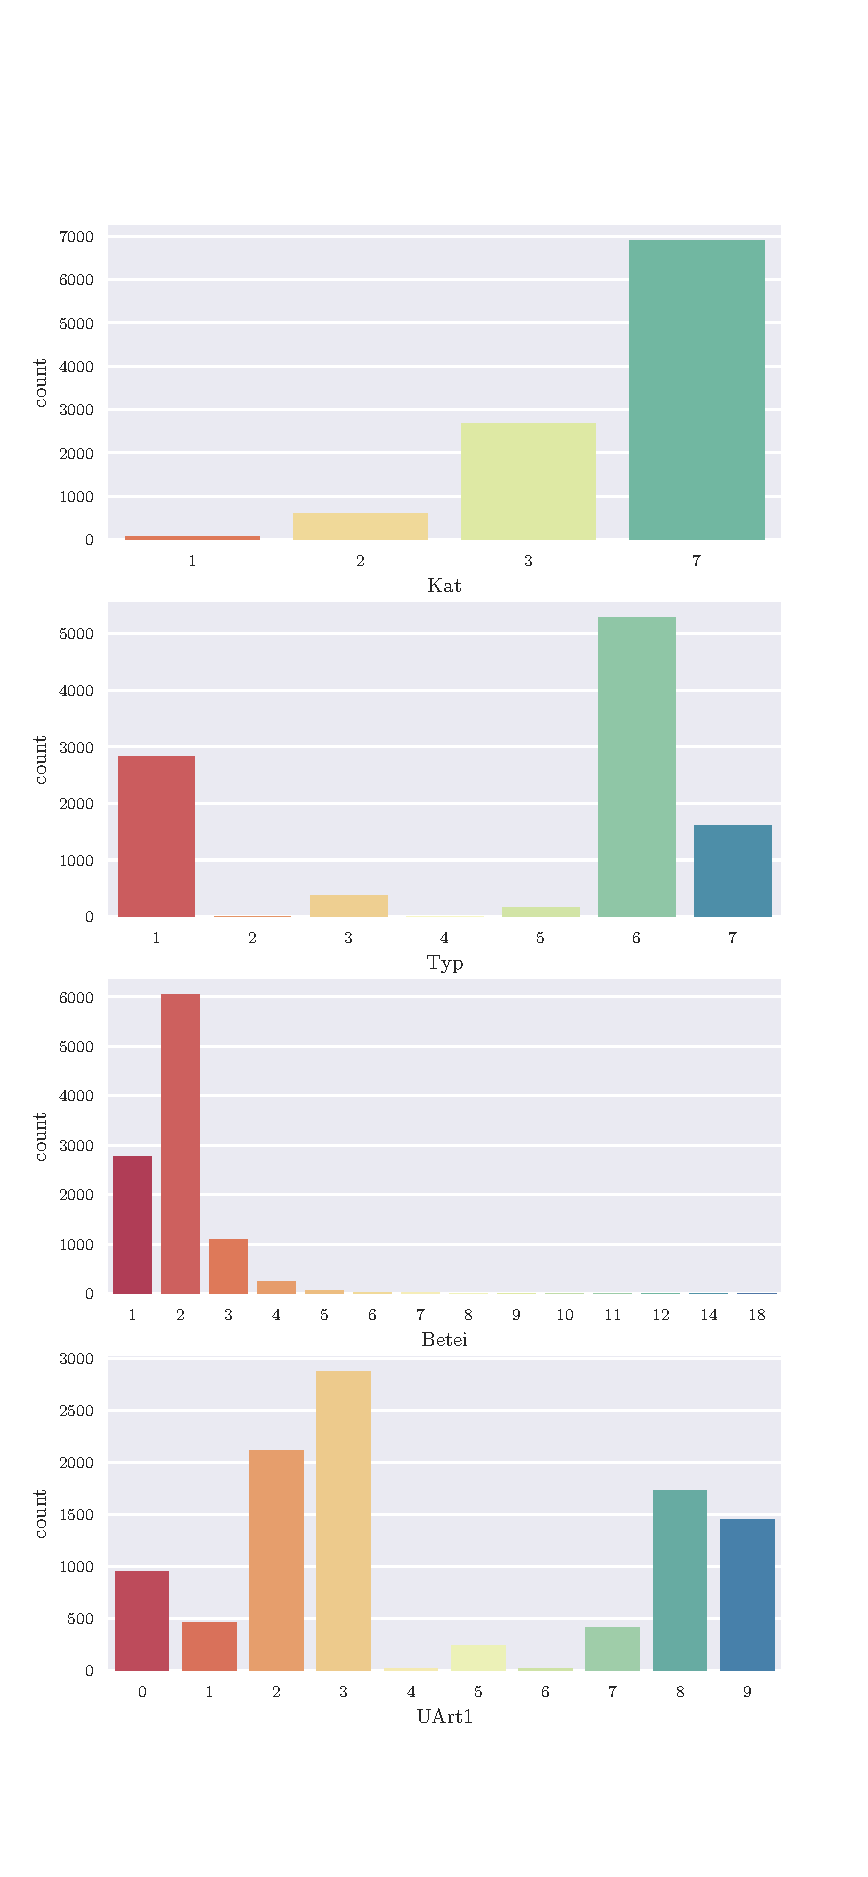
\includegraphics[scale=0.7]{CorrAnalysis/data/BAYSIS/01_dataset/plots/baysis_dataset_count_multiple01}
        \caption{Distribution of the accident category Kat, Typ, Betei and UArt}
        \label{img:baysis_dataset_Kat}
        \label{img:baysis_dataset_Typ}
        \label{img:baysis_dataset_Betei}
        \label{img:baysis_dataset_UArt}
    \end{figure}

    \begin{figure}[ht!]
        \centering
        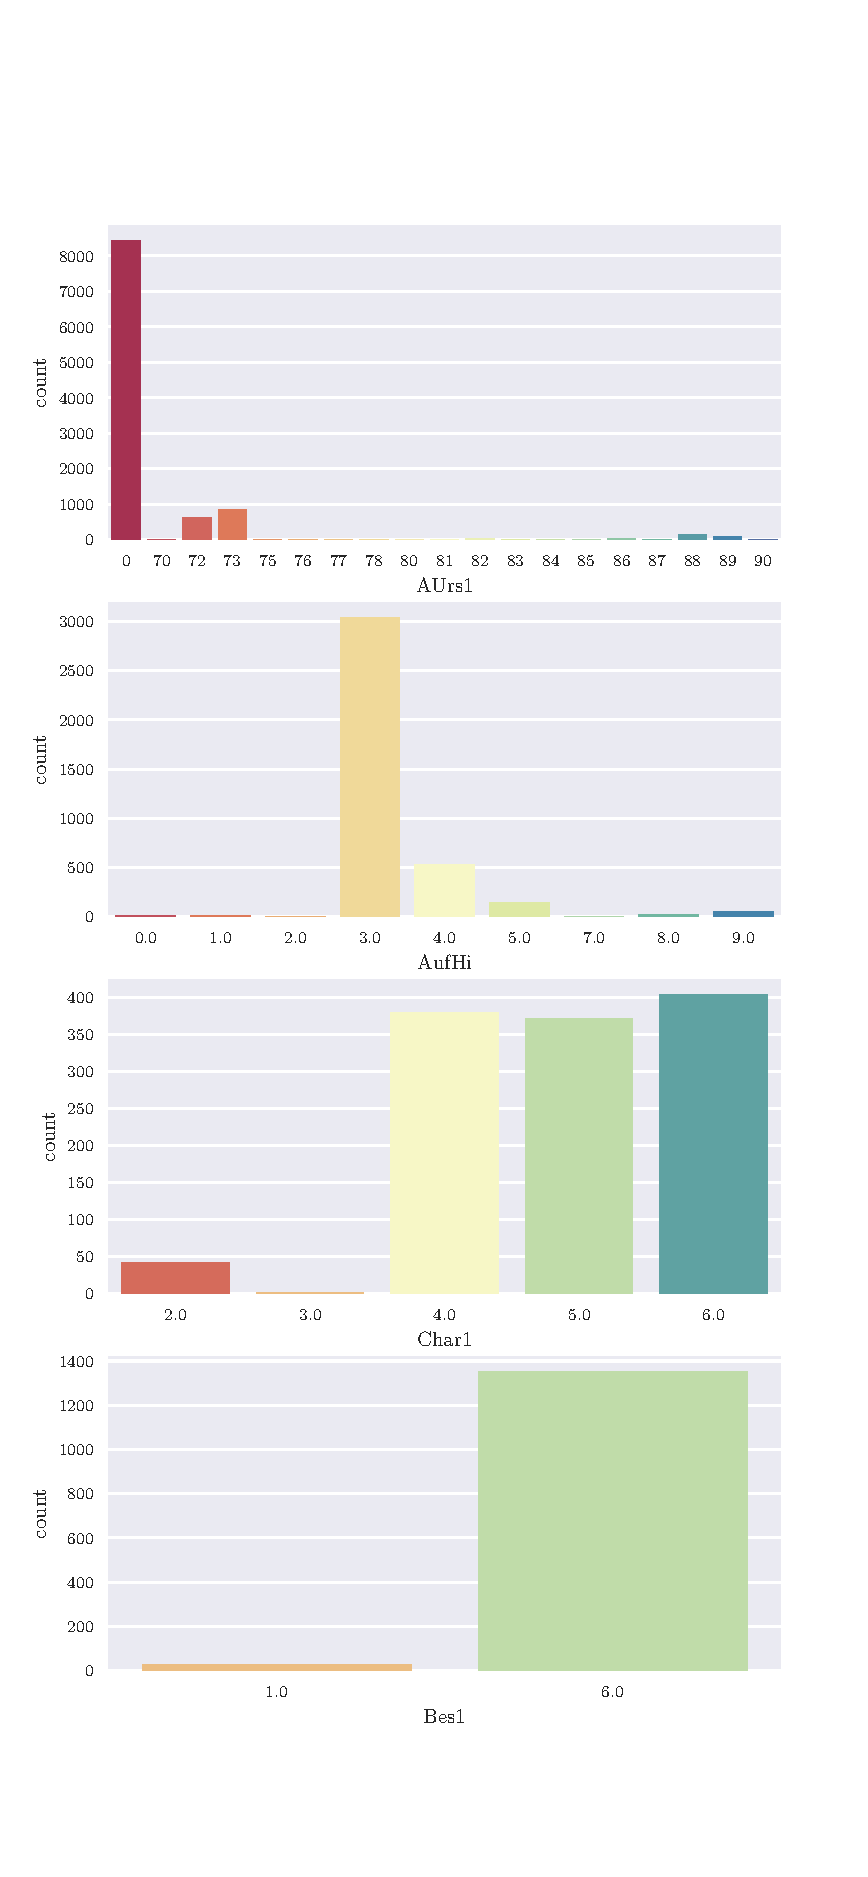
\includegraphics[scale=0.7]{CorrAnalysis/data/BAYSIS/01_dataset/plots/baysis_dataset_count_multiple02}
        \caption{Distribution of the accident category AUrs, AufHi, Char and Bes}
        \label{img:baysis_dataset_AUrs}
        \label{img:baysis_dataset_AufHi}
        \label{img:baysis_dataset_Char}
        \label{img:baysis_dataset_Bes}
    \end{figure}

    \begin{figure}[ht!]
        \centering
        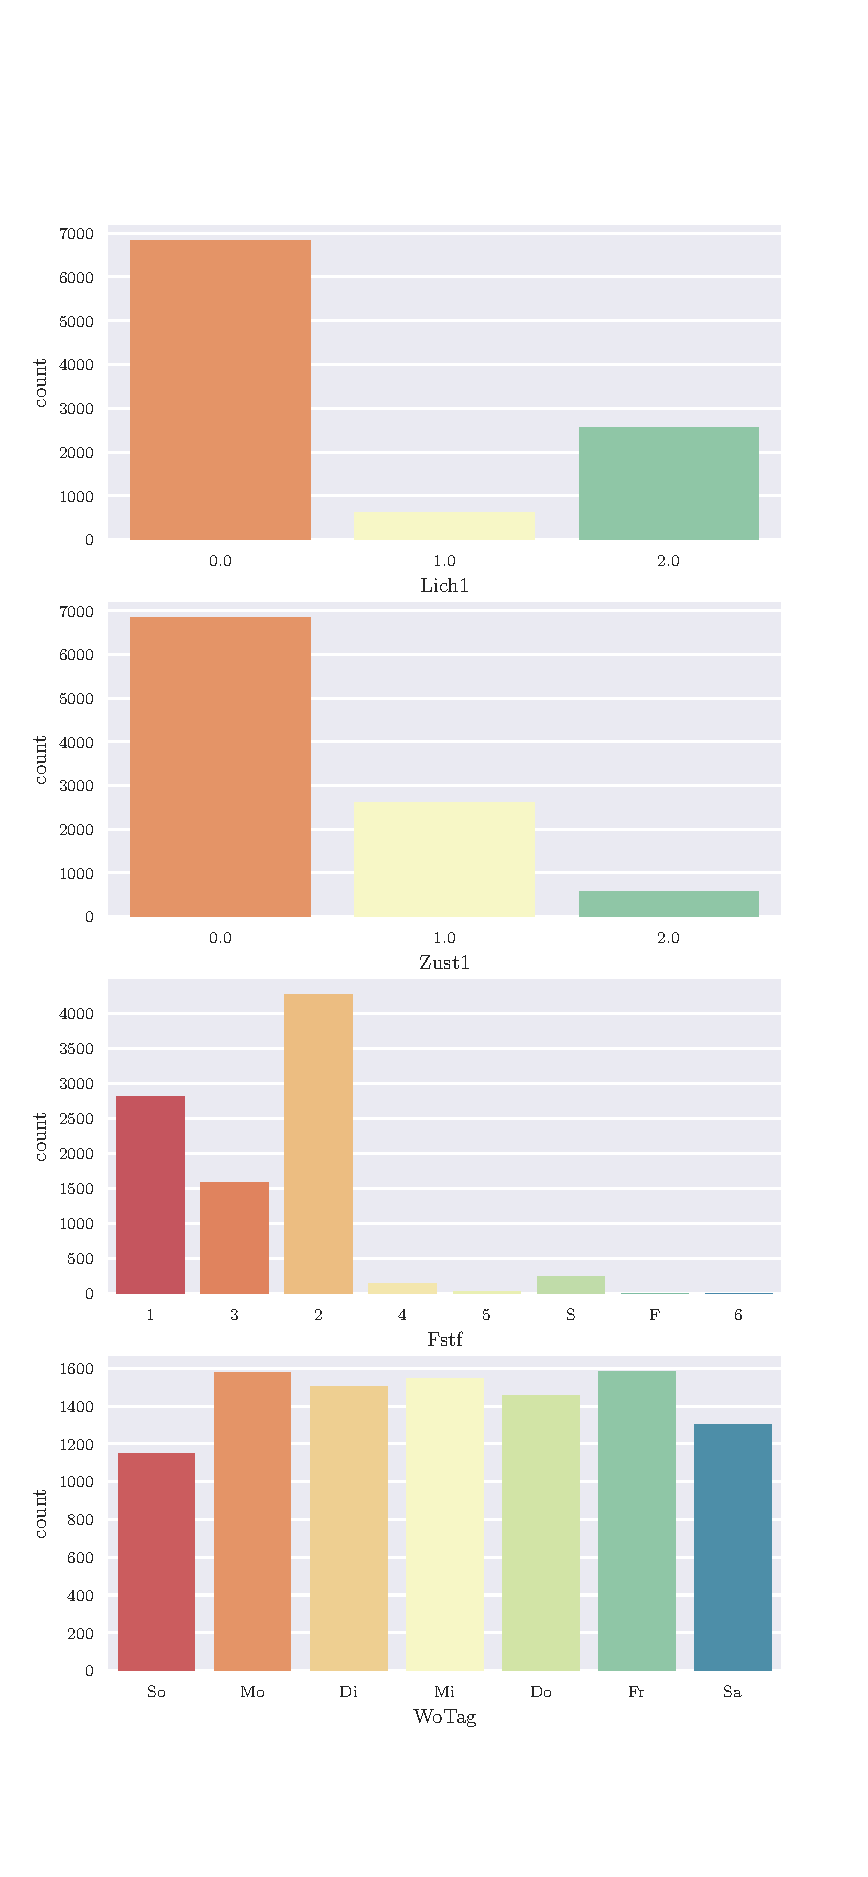
\includegraphics[scale=0.7]{CorrAnalysis/data/BAYSIS/01_dataset/plots/baysis_dataset_count_multiple03}
        \caption{Distribution of the accident category Lich, Zust, Fstf and WoTag}
        \label{img:baysis_dataset_Lich}
        \label{img:baysis_dataset_Zust}
        \label{img:baysis_dataset_Fstf}
        \label{img:baysis_dataset_WoTag}
    \end{figure}

    % ------- BAYSIS Dataset - Tables --------
    % \newgeometry{left=1cm,right=1cm,top=1cm}
    \begin{sidewaystable}
        \tiny
        \setlength{\tabcolsep}{4pt}
        \centering
        \begin{tabular}{lrrrrrrrrrrrrrrrrrrrr}
\toprule
{} &  Strasse &  Kat &  Typ &  Betei &  UArt1 &  UArt2 &  AUrs1 &  AUrs2 &  AufHi &  Alkoh &  Char1 &  Char2 &  Lich1 &  Lich2 &  Zust1 &  Zust2 &  Fstf &  WoTag &  FeiTag &  Month \\
\midrule
Strasse &     1.00 & 0.07 & 0.11 &   0.08 &   0.09 &   0.05 &   0.07 &   0.04 &   0.08 &   0.07 &   0.12 &   0.10 &   0.05 &   0.06 &   0.10 &   0.06 &  0.15 &   0.09 &    0.05 &   0.05 \\
Kat     &     0.07 & 1.00 & 0.16 &   0.18 &   0.31 &   0.10 &   0.08 &   0.05 &   0.12 &   0.02 &   0.05 &   0.03 &   0.02 &   0.04 &   0.05 &   0.02 &  0.08 &   0.04 &    0.03 &   0.05 \\
Typ     &     0.11 & 0.16 & 1.00 &   0.31 &   0.56 &   0.06 &   0.26 &   0.06 &   0.25 &   0.06 &   0.15 &   0.09 &   0.09 &   0.20 &   0.33 &   0.12 &  0.16 &   0.08 &    0.05 &   0.09 \\
Betei   &     0.08 & 0.18 & 0.31 &   1.00 &   0.28 &   0.06 &   0.14 &   0.20 &   0.24 &   0.04 &   0.07 &   0.07 &   0.09 &   0.09 &   0.25 &   0.10 &  0.08 &   0.07 &    0.06 &   0.06 \\
UArt1   &     0.09 & 0.31 & 0.56 &   0.28 &   1.00 &   0.08 &   0.21 &   0.05 &   0.32 &   0.05 &   0.14 &   0.09 &   0.10 &   0.22 &   0.25 &   0.09 &  0.16 &   0.08 &    0.05 &   0.06 \\
UArt2   &     0.05 & 0.10 & 0.06 &   0.06 &   0.08 &   1.00 &   0.06 &   0.03 &   0.15 &   0.04 &   0.03 &   0.05 &   0.03 &   0.05 &   0.08 &   0.04 &  0.04 &   0.04 &    0.01 &   0.04 \\
AUrs1   &     0.07 & 0.08 & 0.26 &   0.14 &   0.21 &   0.06 &   1.00 &   0.20 &   0.16 &   0.05 &   0.08 &   0.09 &   0.12 &   0.13 &   0.66 &   0.77 &  0.05 &   0.09 &    0.04 &   0.15 \\
AUrs2   &     0.04 & 0.05 & 0.06 &   0.20 &   0.05 &   0.03 &   0.20 &   1.00 &   0.06 &   0.04 &   0.03 &   0.06 &   0.04 &   0.03 &   0.12 &   0.33 &  0.03 &   0.03 &    0.03 &   0.05 \\
AufHi   &     0.08 & 0.12 & 0.25 &   0.24 &   0.32 &   0.15 &   0.16 &   0.06 &   1.00 &   0.04 &   0.08 &   0.10 &   0.08 &   0.10 &   0.25 &   0.09 &  0.06 &   0.07 &    0.04 &   0.06 \\
Alkoh   &     0.07 & 0.02 & 0.06 &   0.04 &   0.05 &   0.04 &   0.05 &   0.04 &   0.04 &   1.00 &   0.02 &   0.00 &   0.11 &   0.11 &   0.03 &   0.01 &  0.05 &   0.08 &    0.01 &   0.05 \\
Char1   &     0.12 & 0.05 & 0.15 &   0.07 &   0.14 &   0.03 &   0.08 &   0.03 &   0.08 &   0.02 &   1.00 &   0.58 &   0.04 &   0.05 &   0.10 &   0.03 &  0.06 &   0.03 &    0.02 &   0.04 \\
Char2   &     0.10 & 0.03 & 0.09 &   0.07 &   0.09 &   0.05 &   0.09 &   0.06 &   0.10 &   0.00 &   0.58 &   1.00 &   0.04 &   0.04 &   0.08 &   0.03 &  0.08 &   0.03 &    0.02 &   0.04 \\
Lich1   &     0.05 & 0.02 & 0.09 &   0.09 &   0.10 &   0.03 &   0.12 &   0.04 &   0.08 &   0.11 &   0.04 &   0.04 &   1.00 &   0.71 &   0.16 &   0.06 &  0.05 &   0.04 &    0.03 &   0.21 \\
Lich2   &     0.06 & 0.04 & 0.20 &   0.09 &   0.22 &   0.05 &   0.13 &   0.03 &   0.10 &   0.11 &   0.05 &   0.04 &   0.71 &   1.00 &   0.16 &   0.06 &  0.17 &   0.04 &    0.03 &   0.20 \\
Zust1   &     0.10 & 0.05 & 0.33 &   0.25 &   0.25 &   0.08 &   0.66 &   0.12 &   0.25 &   0.03 &   0.10 &   0.08 &   0.16 &   0.16 &   1.00 &   0.17 &  0.06 &   0.12 &    0.05 &   0.37 \\
Zust2   &     0.06 & 0.02 & 0.12 &   0.10 &   0.09 &   0.04 &   0.77 &   0.33 &   0.09 &   0.01 &   0.03 &   0.03 &   0.06 &   0.06 &   0.17 &   1.00 &  0.05 &   0.06 &    0.02 &   0.17 \\
Fstf    &     0.15 & 0.08 & 0.16 &   0.08 &   0.16 &   0.04 &   0.05 &   0.03 &   0.06 &   0.05 &   0.06 &   0.08 &   0.05 &   0.17 &   0.06 &   0.05 &  1.00 &   0.03 &    0.02 &   0.04 \\
WoTag   &     0.09 & 0.04 & 0.08 &   0.07 &   0.08 &   0.04 &   0.09 &   0.03 &   0.07 &   0.08 &   0.03 &   0.03 &   0.04 &   0.04 &   0.12 &   0.06 &  0.03 &   1.00 &    0.13 &   0.09 \\
FeiTag  &     0.05 & 0.03 & 0.05 &   0.06 &   0.05 &   0.01 &   0.04 &   0.03 &   0.04 &   0.01 &   0.02 &   0.02 &   0.03 &   0.03 &   0.05 &   0.02 &  0.02 &   0.13 &    1.00 &   0.13 \\
Month   &     0.05 & 0.05 & 0.09 &   0.06 &   0.06 &   0.04 &   0.15 &   0.05 &   0.06 &   0.05 &   0.04 &   0.04 &   0.21 &   0.20 &   0.37 &   0.17 &  0.04 &   0.09 &    0.13 &   1.00 \\
\bottomrule
\end{tabular}

        \caption{Correlation matrix for BAYSIS dataset, calculated with Cramer's $V$, $\eta$, $\tau$, $r_{pq}$, $r$}
        \label{table:appendix_correlation_matrix_dataset_cramers}
    \end{sidewaystable}
    \begin{sidewaystable}
        \tiny
        \setlength{\tabcolsep}{4pt}
        \centering
        \begin{tabular}{lrrrrrrrrrrrrrrrrrrrr}
\toprule
{} &  Strasse &  Kat &  Typ &  Betei &  UArt1 &  UArt2 &  AUrs1 &  AUrs2 &  AufHi &  Alkoh &  Char1 &  Char2 &  Lich1 &  Lich2 &  Zust1 &  Zust2 &  Fstf &  WoTag &  FeiTag &  Month \\
\midrule
Strasse &     1.00 & 0.00 & 0.02 &   0.01 &   0.01 &   0.00 &   0.01 &   0.00 &   0.01 &   0.00 &   0.01 &   0.00 &   0.00 &   0.00 &   0.00 &   0.00 &  0.04 &   0.01 &    0.00 &   0.01 \\
Kat     &     0.01 & 1.00 & 0.04 &   0.05 &   0.16 &   0.02 &   0.01 &   0.00 &   0.01 &   0.00 &   0.00 &   0.00 &   0.00 &   0.00 &   0.00 &   0.00 &  0.01 &   0.00 &    0.00 &   0.00 \\
Typ     &     0.03 & 0.03 & 1.00 &   0.26 &   0.39 &   0.01 &   0.15 &   0.01 &   0.17 &   0.00 &   0.02 &   0.00 &   0.01 &   0.02 &   0.09 &   0.01 &  0.05 &   0.02 &    0.00 &   0.02 \\
Betei   &     0.02 & 0.04 & 0.29 &   1.00 &   0.36 &   0.01 &   0.09 &   0.01 &   0.22 &   0.00 &   0.01 &   0.00 &   0.01 &   0.01 &   0.05 &   0.01 &  0.02 &   0.02 &    0.00 &   0.01 \\
UArt1   &     0.02 & 0.07 & 0.25 &   0.20 &   1.00 &   0.02 &   0.07 &   0.00 &   0.25 &   0.00 &   0.01 &   0.00 &   0.01 &   0.01 &   0.03 &   0.00 &  0.05 &   0.01 &    0.00 &   0.01 \\
UArt2   &     0.02 & 0.03 & 0.02 &   0.03 &   0.07 &   1.00 &   0.02 &   0.00 &   0.20 &   0.00 &   0.01 &   0.00 &   0.00 &   0.01 &   0.01 &   0.00 &  0.01 &   0.01 &    0.00 &   0.01 \\
AUrs1   &     0.05 & 0.01 & 0.25 &   0.14 &   0.18 &   0.01 &   1.00 &   0.04 &   0.14 &   0.00 &   0.02 &   0.01 &   0.02 &   0.02 &   0.38 &   0.05 &  0.01 &   0.03 &    0.00 &   0.14 \\
AUrs2   &     0.09 & 0.02 & 0.12 &   0.10 &   0.12 &   0.02 &   0.37 &   1.00 &   0.08 &   0.01 &   0.02 &   0.01 &   0.02 &   0.01 &   0.16 &   0.25 &  0.05 &   0.05 &    0.01 &   0.13 \\
AufHi   &     0.03 & 0.01 & 0.22 &   0.25 &   0.50 &   0.11 &   0.11 &   0.01 &   1.00 &   0.00 &   0.02 &   0.01 &   0.01 &   0.01 &   0.07 &   0.01 &  0.02 &   0.02 &    0.00 &   0.02 \\
Alkoh   &     0.01 & 0.00 & 0.01 &   0.01 &   0.02 &   0.01 &   0.02 &   0.00 &   0.01 &   1.00 &   0.00 &   0.00 &   0.05 &   0.05 &   0.00 &   0.00 &  0.01 &   0.03 &    0.00 &   0.01 \\
Char1   &     0.06 & 0.01 & 0.05 &   0.03 &   0.05 &   0.01 &   0.03 &   0.00 &   0.03 &   0.00 &   1.00 &   0.14 &   0.00 &   0.00 &   0.02 &   0.00 &  0.02 &   0.01 &    0.00 &   0.01 \\
Char2   &     0.05 & 0.00 & 0.03 &   0.02 &   0.03 &   0.01 &   0.03 &   0.01 &   0.04 &   0.00 &   0.60 &   1.00 &   0.01 &   0.01 &   0.03 &   0.00 &  0.02 &   0.00 &    0.00 &   0.01 \\
Lich1   &     0.00 & 0.00 & 0.01 &   0.01 &   0.01 &   0.00 &   0.02 &   0.00 &   0.01 &   0.01 &   0.00 &   0.00 &   1.00 &   0.80 &   0.03 &   0.00 &  0.00 &   0.00 &    0.00 &   0.06 \\
Lich2   &     0.01 & 0.00 & 0.03 &   0.01 &   0.04 &   0.00 &   0.02 &   0.00 &   0.02 &   0.01 &   0.00 &   0.00 &   0.90 &   1.00 &   0.04 &   0.00 &  0.03 &   0.00 &    0.00 &   0.06 \\
Zust1   &     0.01 & 0.00 & 0.14 &   0.08 &   0.08 &   0.01 &   0.36 &   0.02 &   0.08 &   0.00 &   0.01 &   0.00 &   0.03 &   0.03 &   1.00 &   0.04 &  0.00 &   0.02 &    0.00 &   0.14 \\
Zust2   &     0.03 & 0.01 & 0.13 &   0.08 &   0.07 &   0.01 &   0.38 &   0.19 &   0.08 &   0.00 &   0.01 &   0.00 &   0.03 &   0.03 &   0.28 &   1.00 &  0.02 &   0.02 &    0.00 &   0.24 \\
Fstf    &     0.06 & 0.01 & 0.04 &   0.02 &   0.06 &   0.00 &   0.01 &   0.00 &   0.01 &   0.00 &   0.01 &   0.00 &   0.00 &   0.01 &   0.00 &   0.00 &  1.00 &   0.00 &    0.00 &   0.00 \\
WoTag   &     0.01 & 0.00 & 0.01 &   0.01 &   0.01 &   0.00 &   0.01 &   0.00 &   0.01 &   0.00 &   0.00 &   0.00 &   0.00 &   0.00 &   0.01 &   0.00 &  0.00 &   1.00 &    0.00 &   0.01 \\
FeiTag  &     0.01 & 0.00 & 0.01 &   0.01 &   0.01 &   0.00 &   0.01 &   0.00 &   0.01 &   0.00 &   0.00 &   0.00 &   0.00 &   0.00 &   0.01 &   0.00 &  0.00 &   0.07 &    1.00 &   0.10 \\
Month   &     0.01 & 0.00 & 0.01 &   0.01 &   0.01 &   0.00 &   0.04 &   0.00 &   0.01 &   0.00 &   0.00 &   0.00 &   0.02 &   0.02 &   0.04 &   0.01 &  0.00 &   0.01 &    0.00 &   1.00 \\
\bottomrule
\end{tabular}

        \caption{Correlation matrix for BAYSIS dataset, calculated with Theil's $U$, $\eta$, $\tau$, $r_{pq}$, $r$}
        \label{table:appendix_correlation_matrix_dataset_theils}
    \end{sidewaystable}
    \begin{sidewaystable}
        \tiny
        \setlength{\tabcolsep}{4pt}
        \centering
        \begin{tabular}{lrrrrrrrrrrrrrrrrrrrr}
\toprule
{} &  Strasse &   Kat &   Typ &  Betei &  UArt1 &  UArt2 &  AUrs1 &  AUrs2 &  AufHi &  Alkoh &  Char1 &  Char2 &  Lich1 &  Lich2 &  Zust1 &  Zust2 &  Fstf &  WoTag &  FeiTag &  Month \\
\midrule
Strasse &      nan & 0.000 & 0.000 &  0.000 &  0.000 &  0.000 &  0.000 &  0.871 &  0.000 &  0.000 &  0.000 &  0.000 &  0.165 &  0.000 &  0.000 &  0.006 & 0.000 &  0.000 &   0.073 &  0.002 \\
Kat     &    0.000 &   nan & 0.000 &  0.000 &  0.000 &  0.000 &  0.000 &  0.000 &  0.000 &  0.225 &  0.000 &  0.058 &  0.260 &  0.000 &  0.000 &  0.068 & 0.000 &  0.000 &   0.069 &  0.000 \\
Typ     &    0.000 & 0.000 &   nan &  0.000 &  0.000 &  0.000 &  0.000 &  0.000 &  0.000 &  0.000 &  0.000 &  0.000 &  0.000 &  0.000 &  0.000 &  0.000 & 0.000 &  0.000 &   0.000 &  0.000 \\
Betei   &    0.000 & 0.000 & 0.000 &    nan &  0.000 &  0.000 &  0.000 &  0.000 &  0.000 &  0.463 &  0.000 &  0.000 &  0.000 &  0.000 &  0.000 &  0.000 & 0.000 &  0.000 &   0.000 &  0.000 \\
UArt1   &    0.000 & 0.000 & 0.000 &  0.000 &    nan &  0.000 &  0.000 &  0.000 &  0.000 &  0.000 &  0.000 &  0.000 &  0.000 &  0.000 &  0.000 &  0.000 & 0.000 &  0.000 &   0.001 &  0.000 \\
UArt2   &    0.000 & 0.000 & 0.000 &  0.000 &  0.000 &    nan &  0.000 &  0.045 &  0.000 &  0.017 &  0.043 &  0.001 &  0.122 &  0.001 &  0.000 &  0.002 & 0.000 &  0.016 &   0.998 &  0.054 \\
AUrs1   &    0.000 & 0.000 & 0.000 &  0.000 &  0.000 &  0.000 &    nan &  0.000 &  0.000 &  0.157 &  0.000 &  0.000 &  0.000 &  0.000 &  0.000 &  0.000 & 0.002 &  0.000 &   0.386 &  0.000 \\
AUrs2   &    0.871 & 0.000 & 0.000 &  0.000 &  0.000 &  0.045 &  0.000 &    nan &  0.000 &  0.070 &  0.130 &  0.000 &  0.028 &  0.647 &  0.000 &  0.000 & 0.247 &  0.100 &   0.199 &  0.000 \\
AufHi   &    0.000 & 0.000 & 0.000 &  0.000 &  0.000 &  0.000 &  0.000 &  0.000 &    nan &  0.026 &  0.000 &  0.000 &  0.000 &  0.000 &  0.000 &  0.000 & 0.000 &  0.000 &   0.066 &  0.000 \\
Alkoh   &    0.000 & 0.225 & 0.000 &  0.463 &  0.000 &  0.017 &  0.157 &  0.070 &  0.026 &    nan &  0.689 &  0.754 &  0.000 &  0.000 &  0.035 &  0.745 & 0.004 &  0.000 &   0.279 &  0.017 \\
Char1   &    0.000 & 0.000 & 0.000 &  0.000 &  0.000 &  0.043 &  0.000 &  0.130 &  0.000 &  0.689 &    nan &  0.000 &  0.000 &  0.000 &  0.000 &  0.017 & 0.000 &  0.007 &   0.415 &  0.084 \\
Char2   &    0.000 & 0.058 & 0.000 &  0.000 &  0.000 &  0.001 &  0.000 &  0.000 &  0.000 &  0.754 &  0.000 &    nan &  0.001 &  0.000 &  0.000 &  0.012 & 0.000 &  0.250 &   0.020 &  0.075 \\
Lich1   &    0.165 & 0.260 & 0.000 &  0.000 &  0.000 &  0.122 &  0.000 &  0.028 &  0.000 &  0.000 &  0.000 &  0.001 &    nan &  0.000 &  0.000 &  0.000 & 0.000 &  0.002 &   0.015 &  0.000 \\
Lich2   &    0.000 & 0.000 & 0.000 &  0.000 &  0.000 &  0.001 &  0.000 &  0.647 &  0.000 &  0.000 &  0.000 &  0.000 &  0.000 &    nan &  0.000 &  0.000 & 0.000 &  0.001 &   0.033 &  0.000 \\
Zust1   &    0.000 & 0.000 & 0.000 &  0.000 &  0.000 &  0.000 &  0.000 &  0.000 &  0.000 &  0.035 &  0.000 &  0.000 &  0.000 &  0.000 &    nan &  0.000 & 0.000 &  0.000 &   0.000 &  0.000 \\
Zust2   &    0.006 & 0.068 & 0.000 &  0.000 &  0.000 &  0.002 &  0.000 &  0.000 &  0.000 &  0.745 &  0.017 &  0.012 &  0.000 &  0.000 &  0.000 &    nan & 0.000 &  0.000 &   0.125 &  0.000 \\
Fstf    &    0.000 & 0.000 & 0.000 &  0.000 &  0.000 &  0.000 &  0.002 &  0.247 &  0.000 &  0.004 &  0.000 &  0.000 &  0.000 &  0.000 &  0.000 &  0.000 &   nan &  0.033 &   0.660 &  0.081 \\
WoTag   &    0.000 & 0.000 & 0.000 &  0.000 &  0.000 &  0.016 &  0.000 &  0.100 &  0.000 &  0.000 &  0.007 &  0.250 &  0.002 &  0.001 &  0.000 &  0.000 & 0.033 &    nan &   0.000 &  0.000 \\
FeiTag  &    0.073 & 0.069 & 0.000 &  0.000 &  0.001 &  0.998 &  0.386 &  0.199 &  0.066 &  0.279 &  0.415 &  0.020 &  0.015 &  0.033 &  0.000 &  0.125 & 0.660 &  0.000 &     nan &  0.000 \\
Month   &    0.002 & 0.000 & 0.000 &  0.000 &  0.000 &  0.054 &  0.000 &  0.000 &  0.000 &  0.017 &  0.084 &  0.075 &  0.000 &  0.000 &  0.000 &  0.000 & 0.081 &  0.000 &   0.000 &    nan \\
\bottomrule
\end{tabular}

        \caption{Significancy matrix for BAYSIS dataset}
        \label{table:appendix_significancy_matrix_dataset}
    \end{sidewaystable}
    \begin{sidewaystable}
        \tiny
        \setlength{\tabcolsep}{4pt}
        \centering
        \begin{tabular}{lllllllllllllllllllll}
\toprule
{} & Strasse &  Kat &  Typ & Betei & UArt1 & UArt2 & AUrs1 & AUrs2 & AufHi & Alkoh & Char1 & Char2 & Lich1 & Lich2 & Zust1 & Zust2 & Fstf & WoTag & FeiTag & Month \\
\midrule
Strasse &     NaN &  $V$ &  $V$ &   $V$ &   $V$ &   $V$ &   $V$ &   $V$ &   $V$ &   $V$ &   $V$ &   $V$ &   $V$ &   $V$ &   $V$ &   $V$ &  $V$ &   $V$ &    $V$ &   $V$ \\
Kat     &     $V$ &  NaN &  $V$ &   $V$ &   $V$ &   $V$ &   $V$ &   $V$ &   $V$ &   $V$ &   $V$ &   $V$ &   $V$ &   $V$ &   $V$ &   $V$ &  $V$ &   $V$ &    $V$ &   $V$ \\
Typ     &     $V$ &  $V$ &  NaN &   $V$ &   $V$ &   $V$ &   $V$ &   $V$ &   $V$ &   $V$ &   $V$ &   $V$ &   $V$ &   $V$ &   $V$ &   $V$ &  $V$ &   $V$ &    $V$ &   $V$ \\
Betei   &     $V$ &  $V$ &  $V$ &   NaN &   $V$ &   $V$ &   $V$ &   $V$ &   $V$ &   $V$ &   $V$ &   $V$ &   $V$ &   $V$ &   $V$ &   $V$ &  $V$ &   $V$ &    $V$ &   $V$ \\
UArt1   &     $V$ &  $V$ &  $V$ &   $V$ &   NaN &   $V$ &   $V$ &   $V$ &   $V$ &   $V$ &   $V$ &   $V$ &   $V$ &   $V$ &   $V$ &   $V$ &  $V$ &   $V$ &    $V$ &   $V$ \\
UArt2   &     $V$ &  $V$ &  $V$ &   $V$ &   $V$ &   NaN &   $V$ &   $V$ &   $V$ &   $V$ &   $V$ &   $V$ &   $V$ &   $V$ &   $V$ &   $V$ &  $V$ &   $V$ &    $V$ &   $V$ \\
AUrs1   &     $V$ &  $V$ &  $V$ &   $V$ &   $V$ &   $V$ &   NaN &   $V$ &   $V$ &   $V$ &   $V$ &   $V$ &   $V$ &   $V$ &   $V$ &   $V$ &  $V$ &   $V$ &    $V$ &   $V$ \\
AUrs2   &     $V$ &  $V$ &  $V$ &   $V$ &   $V$ &   $V$ &   $V$ &   NaN &   $V$ &   $V$ &   $V$ &   $V$ &   $V$ &   $V$ &   $V$ &   $V$ &  $V$ &   $V$ &    $V$ &   $V$ \\
AufHi   &     $V$ &  $V$ &  $V$ &   $V$ &   $V$ &   $V$ &   $V$ &   $V$ &   NaN &   $V$ &   $V$ &   $V$ &   $V$ &   $V$ &   $V$ &   $V$ &  $V$ &   $V$ &    $V$ &   $V$ \\
Alkoh   &     $V$ &  $V$ &  $V$ &   $V$ &   $V$ &   $V$ &   $V$ &   $V$ &   $V$ &   NaN &   $V$ &   $V$ &   $V$ &   $V$ &   $V$ &   $V$ &  $V$ &   $V$ &    $V$ &   $V$ \\
Char1   &     $V$ &  $V$ &  $V$ &   $V$ &   $V$ &   $V$ &   $V$ &   $V$ &   $V$ &   $V$ &   NaN &   $V$ &   $V$ &   $V$ &   $V$ &   $V$ &  $V$ &   $V$ &    $V$ &   $V$ \\
Char2   &     $V$ &  $V$ &  $V$ &   $V$ &   $V$ &   $V$ &   $V$ &   $V$ &   $V$ &   $V$ &   $V$ &   NaN &   $V$ &   $V$ &   $V$ &   $V$ &  $V$ &   $V$ &    $V$ &   $V$ \\
Lich1   &     $V$ &  $V$ &  $V$ &   $V$ &   $V$ &   $V$ &   $V$ &   $V$ &   $V$ &   $V$ &   $V$ &   $V$ &   NaN &   $V$ &   $V$ &   $V$ &  $V$ &   $V$ &    $V$ &   $V$ \\
Lich2   &     $V$ &  $V$ &  $V$ &   $V$ &   $V$ &   $V$ &   $V$ &   $V$ &   $V$ &   $V$ &   $V$ &   $V$ &   $V$ &   NaN &   $V$ &   $V$ &  $V$ &   $V$ &    $V$ &   $V$ \\
Zust1   &     $V$ &  $V$ &  $V$ &   $V$ &   $V$ &   $V$ &   $V$ &   $V$ &   $V$ &   $V$ &   $V$ &   $V$ &   $V$ &   $V$ &   NaN &   $V$ &  $V$ &   $V$ &    $V$ &   $V$ \\
Zust2   &     $V$ &  $V$ &  $V$ &   $V$ &   $V$ &   $V$ &   $V$ &   $V$ &   $V$ &   $V$ &   $V$ &   $V$ &   $V$ &   $V$ &   $V$ &   NaN &  $V$ &   $V$ &    $V$ &   $V$ \\
Fstf    &     $V$ &  $V$ &  $V$ &   $V$ &   $V$ &   $V$ &   $V$ &   $V$ &   $V$ &   $V$ &   $V$ &   $V$ &   $V$ &   $V$ &   $V$ &   $V$ &  NaN &   $V$ &    $V$ &   $V$ \\
WoTag   &     $V$ &  $V$ &  $V$ &   $V$ &   $V$ &   $V$ &   $V$ &   $V$ &   $V$ &   $V$ &   $V$ &   $V$ &   $V$ &   $V$ &   $V$ &   $V$ &  $V$ &   NaN &    $V$ &   $V$ \\
FeiTag  &     $V$ &  $V$ &  $V$ &   $V$ &   $V$ &   $V$ &   $V$ &   $V$ &   $V$ &   $V$ &   $V$ &   $V$ &   $V$ &   $V$ &   $V$ &   $V$ &  $V$ &   $V$ &    NaN &   $V$ \\
Month   &     $V$ &  $V$ &  $V$ &   $V$ &   $V$ &   $V$ &   $V$ &   $V$ &   $V$ &   $V$ &   $V$ &   $V$ &   $V$ &   $V$ &   $V$ &   $V$ &  $V$ &   $V$ &    $V$ &   NaN \\
\bottomrule
\end{tabular}

        \caption{Coefficient matrix for BAYSIS dataset}
        \label{table:appendix_coefficient_matrix_dataset}
    \end{sidewaystable}
    % \restoregeometry
    
    % -------------------------------
    % ------- BAYSIS Matched --------
    % -------------------------------
    % \tocless\section{BAYSIS Matched Data}
    % \label{appendix_baysis_dataset}
    
    % ------- BAYSIS Matched - Figures --------
    \begin{figure}[ht!]
        \centering
        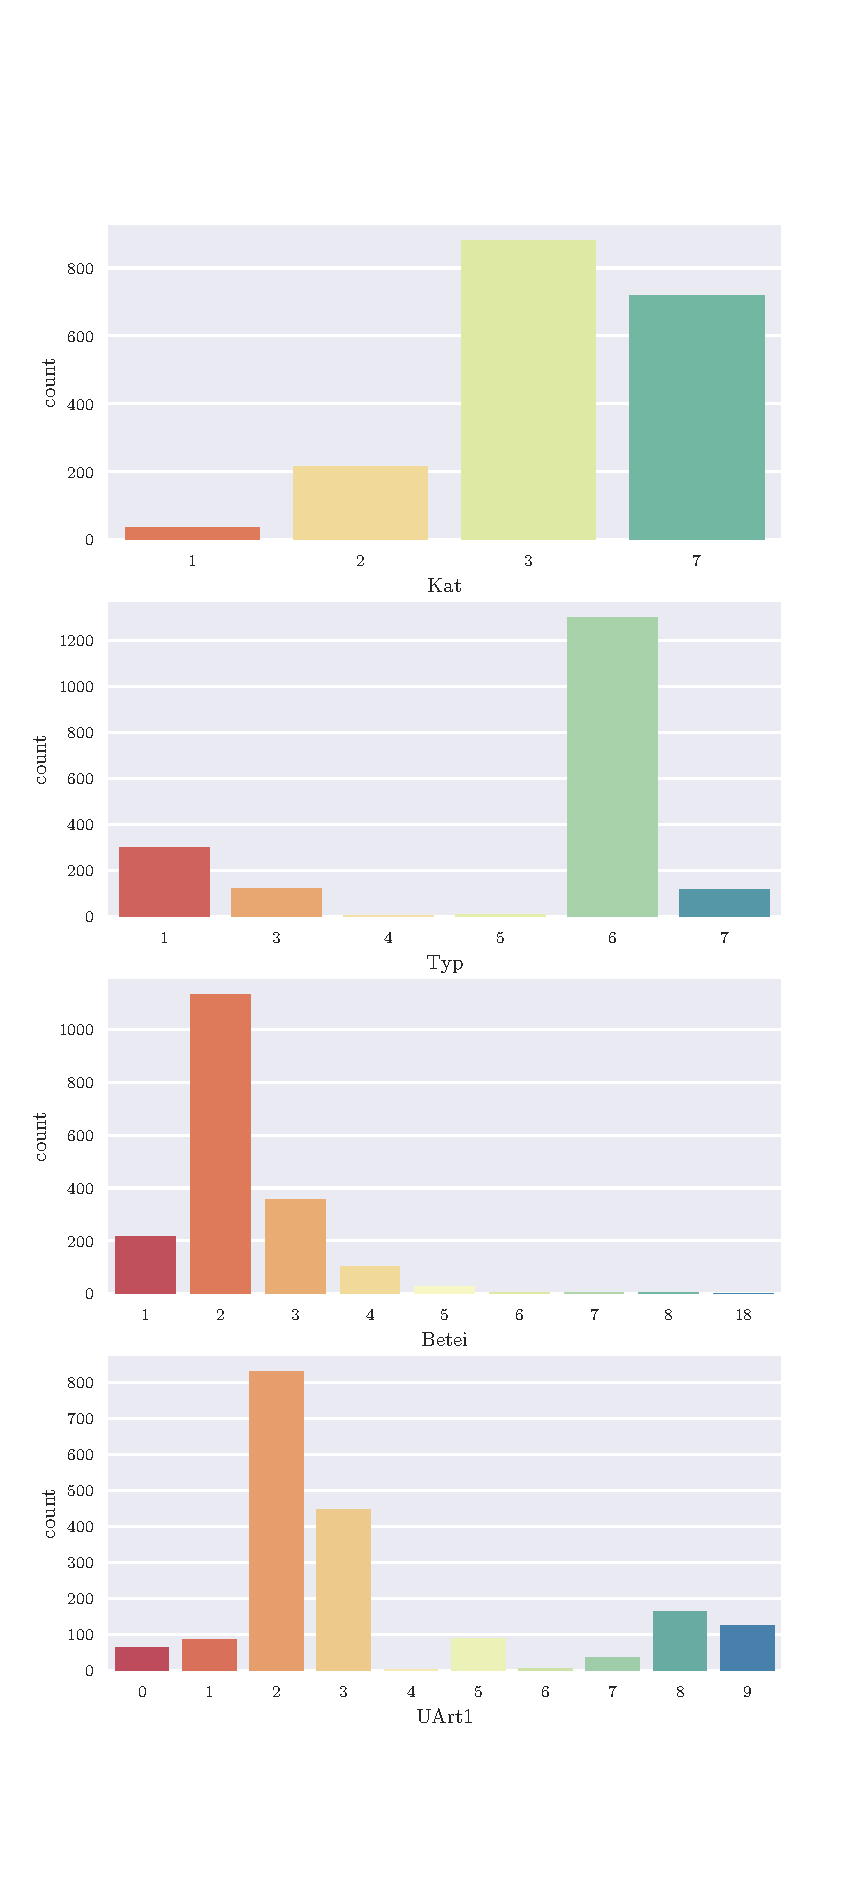
\includegraphics[scale=0.7]{CorrAnalysis/data/BAYSIS/02_matched/plots/baysis_matched_count_multiple01}
        \caption{Distribution of the accident category Kat, Typ, Betei and UArt}
        \label{img:baysis_matched_Kat}
        \label{img:baysis_matched_Typ}
        \label{img:baysis_matched_Betei}
        \label{img:baysis_matched_UArt}
    \end{figure}

    \begin{figure}[ht!]
        \centering
        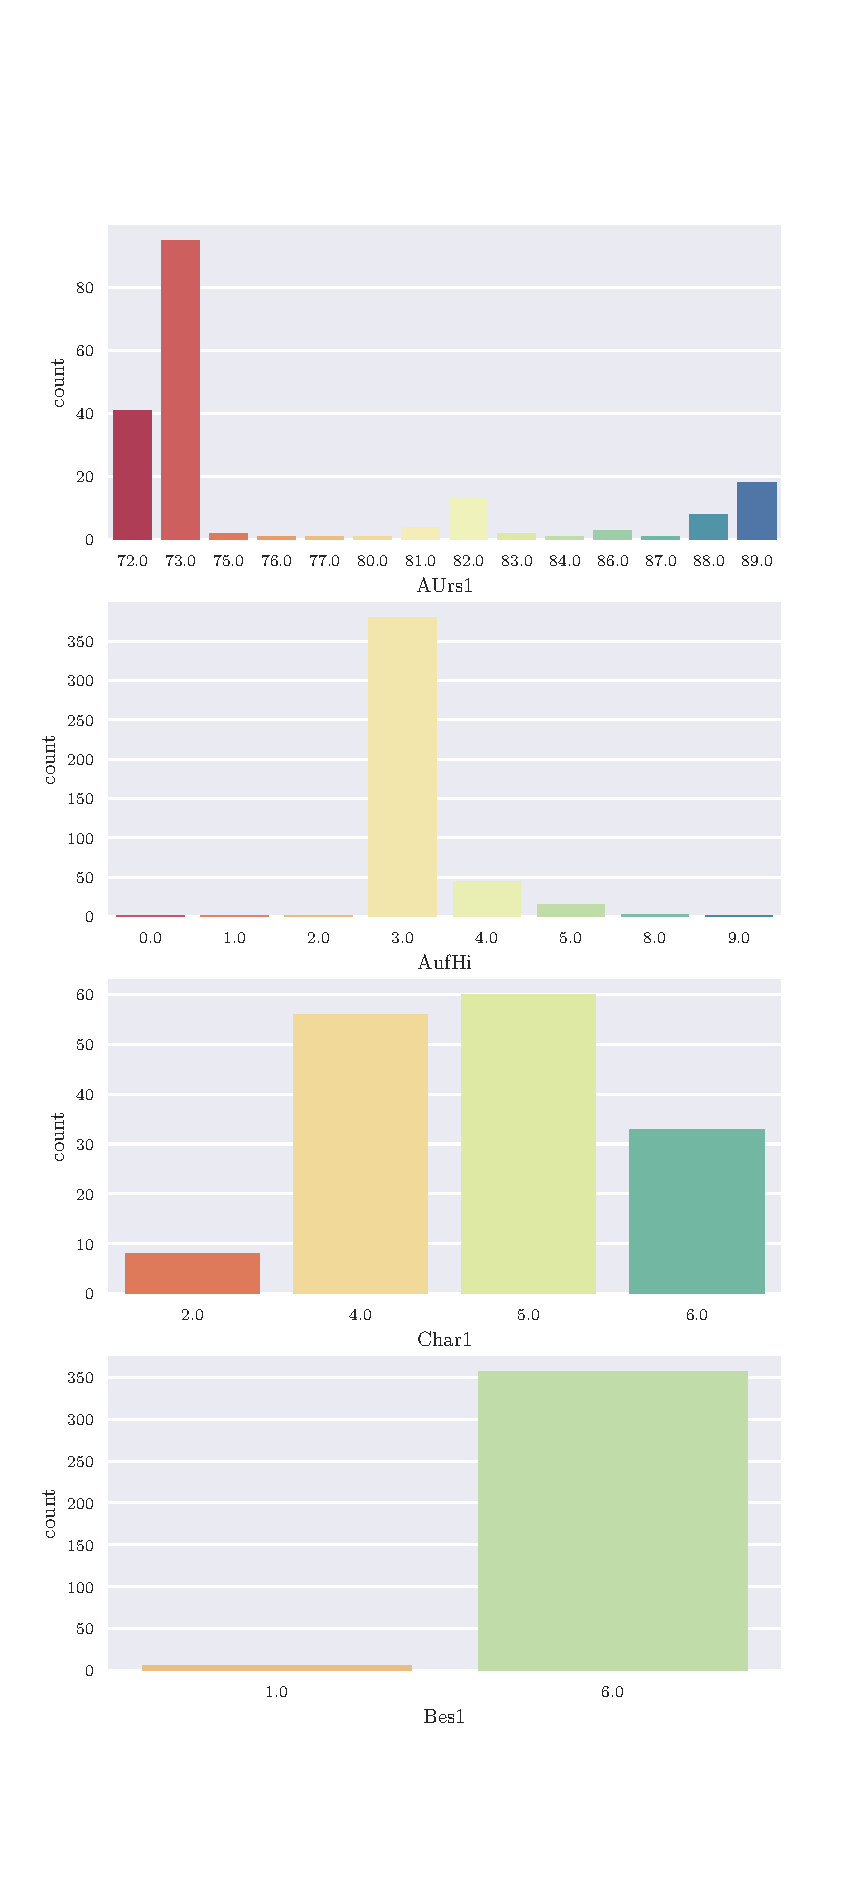
\includegraphics[scale=0.7]{CorrAnalysis/data/BAYSIS/02_matched/plots/baysis_matched_count_multiple02}
        \caption{Distribution of the accident category AUrs, AufHi, Char and Bes}
        \label{img:baysis_matched_AUrs}
        \label{img:baysis_matched_AufHi}
        \label{img:baysis_matched_Char}
        \label{img:baysis_matched_Bes}
    \end{figure}

    \begin{figure}[ht!]
        \centering
        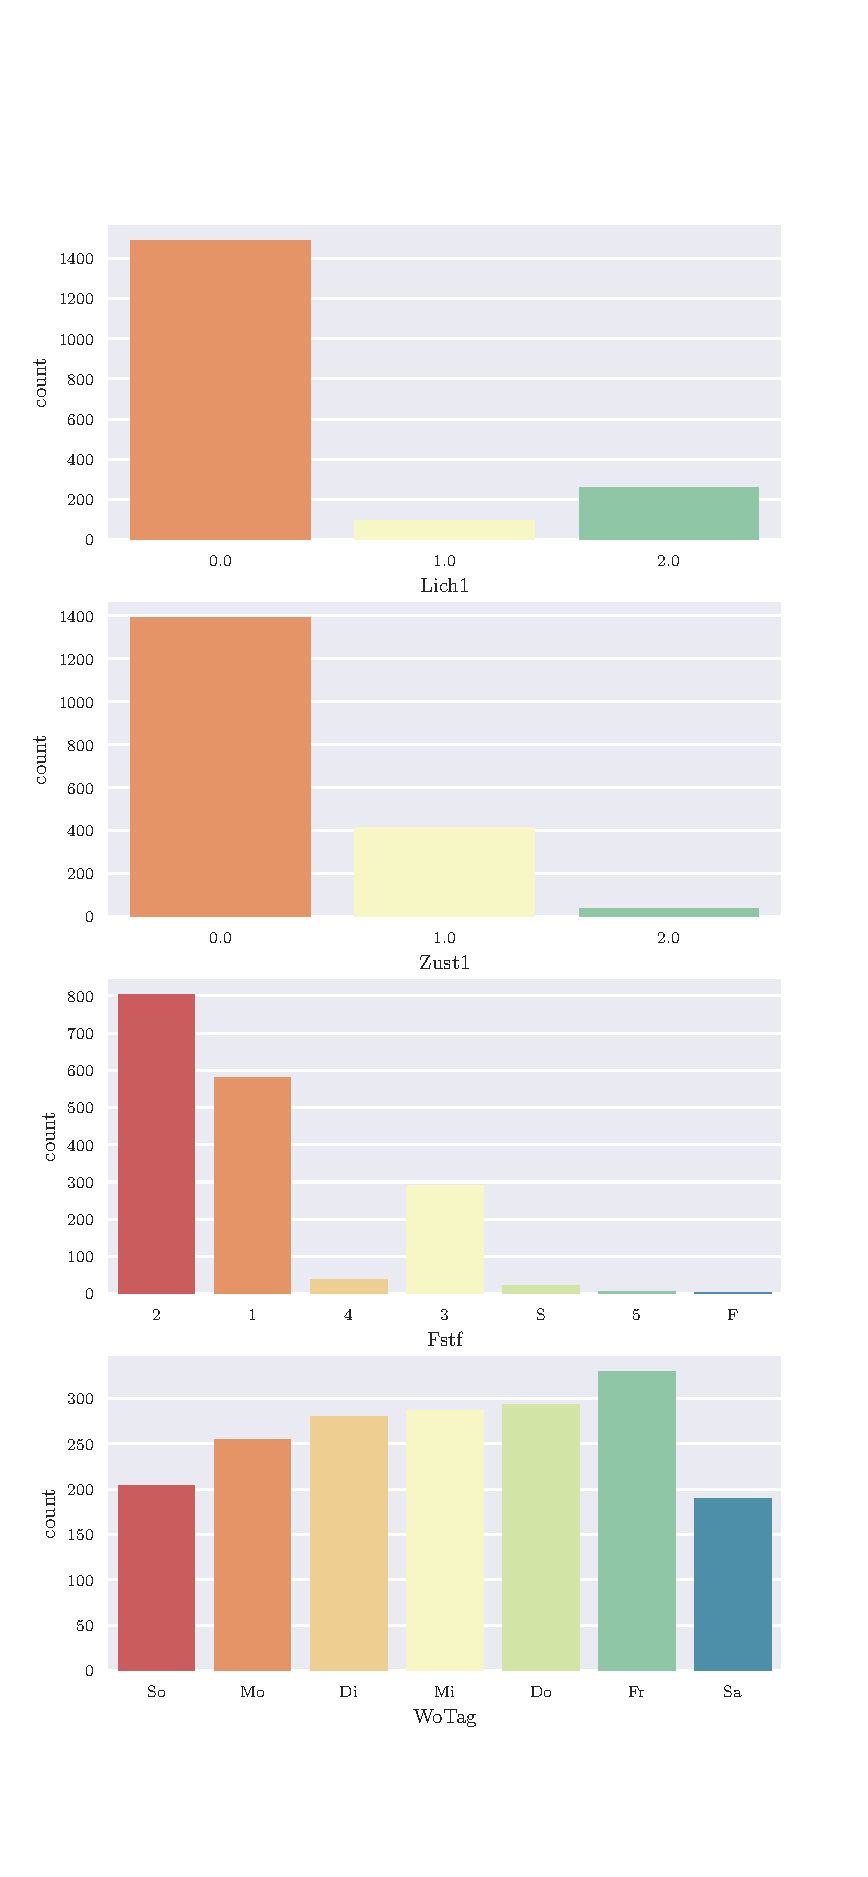
\includegraphics[scale=0.7]{CorrAnalysis/data/BAYSIS/02_matched/plots/baysis_matched_count_multiple03}
        \caption{Distribution of the accident category Lich, Zust, Fstf and WoTag}
        \label{img:baysis_matched_Lich}
        \label{img:baysis_matched_Zust}
        \label{img:baysis_matched_Fstf}
        \label{img:baysis_matched_WoTag}
    \end{figure}

    \begin{table}[ht!]
        \tiny
        \setlength{\tabcolsep}{4pt}
        \centering
        \begin{tabular}{rrrrrrrrrrrrrrrrr}
            \toprule
                    & A3 & A6 & A9 & A70 & A96 & A7 & A73 & A99 & A92 & A93 & A94 & A72 & A995 & A95 & A71 & A45 \\ 
            \midrule
            A6 		& 0.00 &  &  &  &  &  &  &  &  &  &  &  &  &  &  &  \\ 
            A9 		& \red{0.01} & 1.00 &  &  &  &  &  &  &  &  &  &  &  &  &  &  \\ 
            A70 	& \red{0.03} & 1.00 & 1.00 &  &  &  &  &  &  &  &  &  &  &  &  &  \\ 
            A96 	& \red{0.00} & 1.00 & 0.27 & 1.00 &  &  &  &  &  &  &  &  &  &  &  &  \\ 
            A7 		& \red{0.00} & 1.00 & 1.00 & 1.00 & 1.00 &  &  &  &  &  &  &  &  &  &  &  \\ 
            A73 	& \red{0.00} & 1.00 & 0.31 & 1.00 & 1.00 & 1.00 &  &  &  &  &  &  &  &  &  &  \\ 
            A99 	& 1.00 & 1.00 & 1.00 & 1.00 & 0.50 & 1.00 & 0.59 &  &  &  &  &  &  &  &  &  \\ 
            A92 	& \red{0.00} & 1.00 & 0.16 & 1.00 & 1.00 & 1.00 & 1.00 & 0.22 &  &  &  &  &  &  &  &  \\ 
            A93 	& 1.00 & 1.00 & 1.00 & 1.00 & 1.00 & 1.00 & 1.00 & 1.00 & 1.00 &  &  &  &  &  &  &  \\ 
            A94 	& \red{0.01} & 1.00 & 1.00 & 1.00 & 1.00 & 1.00 & 1.00 & 1.00 & 1.00 & 1.00 &  &  &  &  &  &  \\ 
            A72 	& 1.00 & 1.00 & 1.00 & 1.00 & 1.00 & 1.00 & 1.00 & 1.00 & 1.00 & 1.00 & 1.00 &  &  &  &  &  \\ 
            A995 	& 1.00 & 1.00 & 1.00 & 1.00 & 1.00 & 1.00 & 1.00 & 1.00 & 1.00 & 1.00 & 1.00 & 1.00 &  &  &  &  \\ 
            A95 	& 1.00 & 1.00 & 1.00 & 1.00 & 1.00 & 1.00 & 1.00 & 1.00 & 1.00 & 1.00 & 1.00 & 1.00 & 1.00 &  &  &  \\ 
            A71 	& 1.00 & 1.00 & 1.00 & 1.00 & 1.00 & 1.00 & 1.00 & 1.00 & 1.00 & 1.00 & 1.00 & 1.00 & 1.00 & 1.00 &  &  \\ 
            A45 	& 1.00 & 1.00 & 1.00 & 1.00 & 1.00 & 1.00 & 1.00 & 1.00 & 1.00 & 1.00 & 1.00 & 1.00 & 1.00 & 1.00 & 1.00 &  \\ 
            A980 	& 1.00 & 1.00 & 1.00 & 1.00 & 1.00 & 1.00 & 1.00 & 1.00 & 1.00 & 1.00 & 1.00 & 1.00 & 1.00 & 1.00 & 1.00 & 1.00 \\ 
            \bottomrule
        \end{tabular}
        \caption{Pairwise Wilcoxon $T$-test for \textit{Street} and \textit{Maximal Temporal Extent} complete}
        \label{tbl:wilcoxon_baysis_matched_Str_TMax_complete}
    \end{table}

    \begin{table}[ht!]
        \tiny
        \setlength{\tabcolsep}{4pt}
        \centering
        \begin{tabular}{rrrrrrrrrrrrrrrrr}
            \toprule
                    & A3 & A6 & A9 & A70 & A96 & A7 & A73 & A99 & A92 & A93 & A94 & A72 & A995 & A95 & A71 & A45 \\ 
            \midrule
            A6 	 & 0.84 &  &  &  &  &  &  &  &  &  &  &  &  &  &  &  \\ 
            A9 	 & 0.36 & 1.00 &  &  &  &  &  &  &  &  &  &  &  &  &  &  \\ 
            A70	 & 1.00 & 1.00 & 1.00 &  &  &  &  &  &  &  &  &  &  &  &  &  \\ 
            A96  & 0.10 & 1.00 & 1.00 & 1.00 &  &  &  &  &  &  &  &  &  &  &  &  \\ 
            A7 	 & 1.00 & 1.00 & 1.00 & 1.00 & 1.00 &  &  &  &  &  &  &  &  &  &  &  \\ 
            A73  & \red{0.00} & 1.00 & 0.51 & 1.00 & 1.00 & 1.00 &  &  &  &  &  &  &  &  &  &  \\ 
            A99  & \red{0.02} & 1.00 & 1.00 & 1.00 & 1.00 & 1.00 & 1.00 &  &  &  &  &  &  &  &  &  \\ 
            A92  & 0.26 & 1.00 & 1.00 & 1.00 & 1.00 & 1.00 & 1.00 & 1.00 &  &  &  &  &  &  &  &  \\ 
            A93  & 1.00 & 1.00 & 1.00 & 1.00 & 1.00 & 1.00 & 1.00 & 1.00 & 1.00 &  &  &  &  &  &  &  \\ 
            A94  & 0.28 & 1.00 & 1.00 & 1.00 & 1.00 & 1.00 & 1.00 & 1.00 & 1.00 & 1.00 &  &  &  &  &  &  \\ 
            A72  & 1.00 & 1.00 & 1.00 & 1.00 & 1.00 & 1.00 & 1.00 & 1.00 & 1.00 & 1.00 & 1.00 &  &  &  &  &  \\ 
            A995 & 1.00 & 1.00 & 1.00 & 1.00 & 1.00 & 1.00 & 1.00 & 1.00 & 1.00 & 1.00 & 1.00 & 1.00 &  &  &  &  \\ 
            A95  & 1.00 & 1.00 & 1.00 & 1.00 & 1.00 & 1.00 & 1.00 & 1.00 & 1.00 & 1.00 & 1.00 & 1.00 & 1.00 &  &  &  \\ 
            A71	 & 1.00 & 1.00 & 1.00 & 1.00 & 1.00 & 1.00 & 1.00 & 1.00 & 1.00 & 1.00 & 1.00 & 1.00 & 1.00 & 1.00 &  &  \\ 
            A45  & 1.00 & 1.00 & 1.00 & 1.00 & 1.00 & 1.00 & 1.00 & 1.00 & 1.00 & 1.00 & 1.00 & 1.00 & 1.00 & 1.00 & 1.00 &  \\ 
            A980 & 1.00 & 1.00 & 1.00 & 1.00 & 1.00 & 1.00 & 1.00 & 1.00 & 1.00 & 1.00 & 1.00 & 1.00 & 1.00 & 1.00 & 1.00 & 1.00 \\
            \bottomrule
        \end{tabular}
        \caption{Pairwise Wilcoxon $T$-test for \textit{Street} and \textit{Average Temporal Extent} complete}
        \label{tbl:wilcoxon_baysis_matched_Str_TAvg_complete}
    \end{table}

    \begin{table}[ht!]
        \tiny
        \setlength{\tabcolsep}{4pt}
        \centering
        \begin{tabular}{rrrrrrrrrrrrrrrrr}
            \toprule
                    & A3   & A6   & A9   & A70  & A96  & A7   & A73   & A99 & A92 & A93 & A94 & A72 & A995 & A95 & A71 & A45 \\ 
            \midrule
            A6 		& 0.40 &  &  &  &  &  &  &  &  &  &  &  &  &  &  &  \\ 
            A9 		& \red{0.00} & 1.00 &  &  &  &  &  &  &  &  &  &  &  &  &  &  \\ 
            A70 	& \red{0.00} & 0.83 & 0.54 &  &  &  &  &  &  &  &  &  &  &  &  &  \\ 
            A96 	& \red{0.00} & 1.00 & 0.14 & 1.00 &  &  &  &  &  &  &  &  &  &  &  &  \\ 
            A7 		& \red{0.00} & 1.00 & 1.00 & 1.00 & 1.00 &  &  &  &  &  &  &  &  &  &  &  \\ 
            A73 	& \red{0.00} & \red{0.00} & \red{0.00} & 1.00 & 1.00 & 0.59 &  &  &  &  &  &  &  &  &  &  \\ 
            A99 	& 1.00 & 1.00 & 1.00 & 0.80 & 0.31 & 1.00 & \red{0.00} &  &  &  &  &  &  &  &  &  \\ 
            A92 	& \red{0.00} & \red{0.00} & \red{0.00} & 1.00 & 1.00 & 1.00 & 1.00 & \red{0.00} &  &  &  &  &  &  &  &  \\ 
            A93 	& \red{0.03} & 1.00 & 1.00 & 1.00 & 1.00 & 1.00 & 1.00 & 1.00 & 1.00 &  &  &  &  &  &  &  \\ 
            A94 	& \red{0.00} & 0.11 & \red{0.03} & 1.00 & 1.00 & 1.00 & 1.00 & 0.09 & 1.00 & 1.00 &  &  &  &  &  &  \\ 
            A72 	& 1.00 & 1.00 & 1.00 & 1.00 & 1.00 & 1.00 & 1.00 & 1.00 & 1.00 & 1.00 & 1.00 &  &  &  &  &  \\ 
            A995 	& 1.00 & 1.00 & 1.00 & 1.00 & 1.00 & 1.00 & 1.00 & 1.00 & 1.00 & 1.00 & 1.00 & 1.00 &  &  &  &  \\ 
            A95 	& 1.00 & 1.00 & 1.00 & 1.00 & 1.00 & 1.00 & 1.00 & 1.00 & 1.00 & 1.00 & 1.00 & 1.00 & 1.00 &  &  &  \\ 
            A71 	& 1.00 & 1.00 & 1.00 & 1.00 & 1.00 & 1.00 & 1.00 & 1.00 & 1.00 & 1.00 & 1.00 & 1.00 & 1.00 & 1.00 &  &  \\ 
            A45 	& 1.00 & 1.00 & 1.00 & 1.00 & 1.00 & 1.00 & 1.00 & 1.00 & 1.00 & 1.00 & 1.00 & 1.00 & 1.00 & 1.00 & 1.00 &  \\ 
            A980 	& 1.00 & 1.00 & 1.00 & 1.00 & 1.00 & 1.00 & 1.00 & 1.00 & 1.00 & 1.00 & 1.00 & 1.00 & 1.00 & 1.00 & 1.00 & 1.00 \\ 
            \bottomrule
        \end{tabular}
        \caption{Pairwise Wilcoxon $T$-test for \textit{Street} and \textit{Maximal Spatial Extent} complete}
        \label{tbl:wilcoxon_baysis_matched_Str_SMax_complete}
    \end{table}

    \begin{table}[ht!]
        \tiny
        \setlength{\tabcolsep}{4pt}
        \centering
        \begin{tabular}{rrrrrrrrrrrrrrrrr}
            \toprule
                & A3 & A6 & A9 & A70 & A96 & A7 & A73 & A99 & A92 & A93 & A94 & A72 & A995 & A95 & A71 & A45 \\ 
            \midrule
            A6   & 1.00 &  &  &  &  &  &  &  &  &  &  &  &  &  &  &  \\ 
            A9   & 1.00 & 1.00 &  &  &  &  &  &  &  &  &  &  &  &  &  &  \\ 
            A70  & \red{0.05} & 0.83 & 0.71 &  &  &  &  &  &  &  &  &  &  &  &  &  \\ 
            A96  & \red{0.05} & 1.00 & 1.00 & 1.00 &  &  &  &  &  &  &  &  &  &  &  &  \\ 
            A7   & 1.00 & 1.00 & 1.00 & 1.00 & 1.00 &  &  &  &  &  &  &  &  &  &  &  \\ 
            A73  & \red{0.00} & \red{0.00} & \red{0.00} & 1.00 & \red{0.00} & \red{0.00} &  &  &  &  &  &  &  &  &  &  \\ 
            A99  & \red{0.00} & 1.00 & 0.06 & 1.00 & 1.00 & 1.00 & 0.51 &  &  &  &  &  &  &  &  &  \\ 
            A92  & \red{0.00} & 0.61 & \red{0.03} & 1.00 & 1.00 & 1.00 & 1.00 & 1.00 &  &  &  &  &  &  &  &  \\ 
            A93  & \red{0.03} & 0.46 & 0.16 & 1.00 & 1.00 & 1.00 & 1.00 & 1.00 & 1.00 &  &  &  &  &  &  &  \\ 
            A94  & \red{0.00} & 0.07 & 0.01 & 1.00 & 0.36 & 0.31 & 1.00 & 1.00 & 1.00 & 1.00 &  &  &  &  &  &  \\ 
            A72  & 1.00 & 1.00 & 1.00 & 1.00 & 1.00 & 1.00 & 1.00 & 1.00 & 1.00 & 1.00 & 1.00 &  &  &  &  &  \\ 
            A995 & 1.00 & 1.00 & 1.00 & 1.00 & 1.00 & 1.00 & 1.00 & 1.00 & 1.00 & 1.00 & 1.00 & 1.00 &  &  &  &  \\ 
            A95  & 1.00 & 1.00 & 1.00 & 1.00 & 1.00 & 1.00 & 1.00 & 1.00 & 1.00 & 1.00 & 1.00 & 1.00 & 1.00 &  &  &  \\ 
            A71  & 1.00 & 1.00 & 1.00 & 1.00 & 1.00 & 1.00 & 1.00 & 1.00 & 1.00 & 1.00 & 1.00 & 1.00 & 1.00 & 1.00 &  &  \\ 
            A45  & 1.00 & 1.00 & 1.00 & 1.00 & 1.00 & 1.00 & 1.00 & 1.00 & 1.00 & 1.00 & 1.00 & 1.00 & 1.00 & 1.00 & 1.00 &  \\ 
            A980 & 1.00 & 1.00 & 1.00 & 1.00 & 1.00 & 1.00 & 1.00 & 1.00 & 1.00 & 1.00 & 1.00 & 1.00 & 1.00 & 1.00 & 1.00 & 1.00 \\ 
            \bottomrule
        \end{tabular}
        \caption{Pairwise Wilcoxon $T$-test for \textit{Street} and \textit{Average Spatial Extent} complete}
        \label{tbl:wilcoxon_baysis_matched_Str_SAvg_complete}
    \end{table}

    \begin{table}[ht!]
        \tiny
        \setlength{\tabcolsep}{4pt}
        \centering
        \begin{tabular}{rrrrrrrrrrrrrrrrr}
            \toprule
                    & A3   & A6   & A9   & A70  & A96  & A7   & A73 & A99 & A92 & A93 & A94 & A72 & A995 & A95 & A71 & A45 \\ 
            \midrule
            A6 		& \red{0.05} &  &  &  &  &  &  &  &  &  &  &  &  &  &  &  \\ 
            A9 		& \red{0.00} & 1.00 &  &  &  &  &  &  &  &  &  &  &  &  &  &  \\ 
            A70 	& 1.00 & 1.00 & 1.00 &  &  &  &  &  &  &  &  &  &  &  &  &  \\ 
            A96 	& \red{0.00} & 1.00 & \red{0.00} & 1.00 &  &  &  &  &  &  &  &  &  &  &  &  \\ 
            A7 		& \red{0.00} & 1.00 & \red{0.01} & 1.00 & 1.00 &  &  &  &  &  &  &  &  &  &  &  \\ 
            A73 	& \red{0.04} & 1.00 & 1.00 & 1.00 & 1.00 & 1.00 &  &  &  &  &  &  &  &  &  &  \\ 
            A99 	& 0.88 & \red{0.00} & \red{0.00} & 0.09 & \red{0.00} & \red{0.00} & \red{0.00} &  &  &  &  &  &  &  &  &  \\ 
            A92 	& \red{0.00} & 1.00 & 0.12 & 1.00 & 1.00 & 1.00 & 1.00 & \red{0.00} &  &  &  &  &  &  &  &  \\ 
            A93 	& 1.00 & 1.00 & 1.00 & 1.00 & 1.00 & 1.00 & 1.00 & 1.00 & 1.00 &  &  &  &  &  &  &  \\ 
            A94 	& 1.00 & 1.00 & 1.00 & 1.00 & 1.00 & 1.00 & 1.00 & 0.13 & 1.00 & 1.00 &  &  &  &  &  &  \\ 
            A72 	& 1.00 & 1.00 & 1.00 & 1.00 & 1.00 & 1.00 & 1.00 & 1.00 & 1.00 & 1.00 & 1.00 &  &  &  &  &  \\ 
            A995 	& 1.00 & 1.00 & 1.00 & 1.00 & 1.00 & 1.00 & 1.00 & 1.00 & 1.00 & 1.00 & 1.00 & 1.00 &  &  &  &  \\ 
            A95 	& 1.00 & 1.00 & 1.00 & 1.00 & 1.00 & 1.00 & 1.00 & 1.00 & 1.00 & 1.00 & 1.00 & 1.00 & 1.00 &  &  &  \\ 
            A71 	& 1.00 & 1.00 & 1.00 & 1.00 & 1.00 & 1.00 & 1.00 & 1.00 & 1.00 & 1.00 & 1.00 & 1.00 & 1.00 & 1.00 &  &  \\ 
            A45 	& 1.00 & 1.00 & 1.00 & 1.00 & 1.00 & 1.00 & 1.00 & 1.00 & 1.00 & 1.00 & 1.00 & 1.00 & 1.00 & 1.00 & 1.00 &  \\ 
            A980 	& 1.00 & 1.00 & 1.00 & 1.00 & 1.00 & 1.00 & 1.00 & 1.00 & 1.00 & 1.00 & 1.00 & 1.00 & 1.00 & 1.00 & 1.00 & 1.00 \\ 
            \bottomrule
        \end{tabular}
        \caption{Pairwise Wilcoxon $T$-test for \textit{Street} and \textit{Coverage} complete}
        \label{tbl:wilcoxon_baysis_matched_Str_Cov_complete}
    \end{table}

    \begin{table}[ht!]
        \tiny
        \centering
        \begin{tabular}{rrrrrrrrrr}
              \toprule
              & 0 & 1 & 2 & 3 & 4 & 5 & 6 & 7 & 8 \\ 
            \midrule
            % 1 & 1.00 &  &  &  &  &  &  &  &  \\ 
            % 2 & 1.00 & 1.00 &  &  &  &  &  &  &  \\ 
            % 3 & 1.00 & 1.00 & 1.00 &  &  &  &  &  &  \\ 
            % 4 & 0.57 & 0.22 & 0.31 & 0.17 &  &  &  &  &  \\ 
            5 & \red{0.04} & 0.17 & \red{0.00} & \red{0.00} & \red{0.01} &  &  &  &  \\ 
            6 & 0.40 & 0.19 & 0.23 & 0.16 & 1.00 & \red{0.01} &  &  &  \\ 
            7 & \red{0.00} & \red{0.00} & \red{0.00} & \red{0.00} & 1.00 & \red{0.00} & 1.00 &  &  \\ 
            8 & \red{0.02} & \red{0.00} & \red{0.00} & \red{0.00} & 1.00 & \red{0.00} & 1.00 & 0.32 &  \\ 
            9 & \red{0.01} & \red{0.00} & \red{0.00} & \red{0.00} & 1.00 & \red{0.00} & 1.00 & 0.50 & 1.00 \\ 
            \bottomrule
        \end{tabular}
        \caption{Pairwise Wilcoxon $T$-test for \textit{UArt} and \textit{Temporal Distance} complete}
        \label{tbl:wilcoxon_baysis_matched_UArt1_TDist_complete}
    \end{table}

    \begin{table}[ht!]
        \tiny
        \centering
        \begin{tabular}{rrrrrrrrrr}
            \toprule
              & 0 & 1 & 2 & 3 & 4 & 5 & 6 & 7 & 8 \\ 
            \midrule
            % 1 & 1.00 &  &  &  &  &  &  &  &  \\ 
            % 2 & 1.00 & 1.00 &  &  &  &  &  &  &  \\ 
            % 3 & 1.00 & 1.00 & 1.00 &  &  &  &  &  &  \\ 
            % 4 & 1.00 & 1.00 & 1.00 & 1.00 &  &  &  &  &  \\ 
            5 & 0.41 & 0.10 & \red{0.00} & \red{0.01} & 0.65 &  &  &  &  \\ 
            % 6 & 1.00 & 1.00 & 1.00 & 1.00 & 1.00 & 1.00 &  &  &  \\ 
            7 & 0.30 & 0.36 & 0.12 & \red{0.05} & 1.00 & \red{0.00} & 1.00 &  &  \\ 
            8 & \red{0.01} & \red{0.01} & \red{0.00} & \red{0.00} & 1.00 & \red{0.00} & 1.00 & 1.00 &  \\ 
            9 & \red{0.05} & 0.07 & \red{0.00} & \red{0.00} & 1.00 & \red{0.00} & 1.00 & 1.00 & 1.00 \\ 
            \bottomrule
        \end{tabular}
        \caption{Pairwise Wilcoxon $T$-test for \textit{UArt} and \textit{Coverage} complete}
        \label{tbl:wilcoxon_baysis_matched_UArt1_Cov_complete}
    \end{table}

    % ------- BAYSIS Matched - Tables --------
    % \newgeometry{left=1cm,right=1cm,bottom=2cm}
    \begin{sidewaystable}
    	\tiny
    	\setlength{\tabcolsep}{2pt}
    	\centering
    	\begin{tabular}{lrrrrrrrrrrrrrrrrrrrrrrrrrrrrr}
\toprule
{} &  TMax &  TAvg &  SMax &  SAvg &  TDist &  SDist &   Cov &  TLCar &  TLHGV &  Str &  Kat &  Typ &  Betei &  UArt1 &  UArt2 &  AUrs1 &  AUrs2 &  AufHi &  Alkoh &  Char1 &  Char2 &  Lich1 &  Lich2 &  Zust1 &  Zust2 &  Fstf &  WoTag &  FeiTag &  Month \\
\midrule
TMax   &  1.00 &  0.82 &  0.58 &  0.49 &  -0.29 &  -0.09 & -0.25 &   0.03 &  -0.01 & 0.25 & 0.15 & 0.06 &   0.09 &   0.12 &   0.08 &   0.14 &   0.06 &   0.14 &  -0.01 &   0.05 &   0.04 &   0.03 &   0.03 &   0.11 &   0.01 & -0.00 &   0.10 &   -0.00 &   0.14 \\
TAvg   &  0.82 &  1.00 &  0.30 &  0.51 &  -0.16 &  -0.07 &  0.10 &   0.02 &  -0.01 & 0.17 & 0.16 & 0.06 &   0.08 &   0.09 &   0.05 &   0.11 &   0.08 &   0.14 &   0.02 &   0.01 &   0.02 &   0.03 &   0.02 &   0.06 &   0.05 &  0.01 &   0.09 &   -0.01 &   0.10 \\
SMax   &  0.58 &  0.30 &  1.00 &  0.64 &  -0.27 &  -0.09 & -0.50 &   0.01 &  -0.05 & 0.31 & 0.10 & 0.09 &   0.08 &   0.18 &   0.08 &   0.14 &   0.06 &   0.13 &  -0.04 &   0.05 &   0.03 &   0.08 &   0.07 &   0.08 &   0.05 &  0.03 &   0.08 &   -0.00 &   0.15 \\
SAvg   &  0.49 &  0.51 &  0.64 &  1.00 &  -0.09 &  -0.13 &  0.10 &   0.01 &  -0.06 & 0.25 & 0.23 & 0.10 &   0.09 &   0.19 &   0.06 &   0.17 &   0.11 &   0.06 &  -0.02 &   0.04 &   0.00 &   0.02 &   0.02 &   0.01 &   0.12 &  0.04 &   0.11 &    0.01 &   0.11 \\
TDist  & -0.29 & -0.16 & -0.27 & -0.09 &   1.00 &   0.05 &  0.31 &  -0.02 &   0.02 & 0.17 & 0.19 & 0.24 &  -0.04 &   0.29 &   0.11 &   0.20 &   0.11 &   0.21 &   0.04 &   0.11 &   0.11 &   0.13 &   0.14 &   0.13 &   0.02 &  0.03 &   0.10 &    0.01 &   0.10 \\
SDist  & -0.09 & -0.07 & -0.09 & -0.13 &   0.05 &   1.00 & -0.04 &  -0.02 &   0.02 & 0.22 & 0.10 & 0.05 &  -0.03 &   0.07 &   0.06 &   0.15 &   0.02 &   0.02 &  -0.03 &   0.07 &   0.02 &   0.05 &   0.05 &   0.05 &   0.01 &  0.04 &   0.08 &   -0.00 &   0.07 \\
Cov    & -0.25 &  0.10 & -0.50 &  0.10 &   0.31 &  -0.04 &  1.00 &  -0.00 &   0.01 & 0.29 & 0.13 & 0.21 &  -0.02 &   0.24 &   0.12 &   0.22 &   0.10 &   0.21 &   0.07 &   0.11 &   0.08 &   0.15 &   0.15 &   0.17 &   0.03 &  0.02 &   0.16 &    0.01 &   0.14 \\
TLCar  &  0.03 &  0.02 &  0.01 &  0.01 &  -0.02 &  -0.02 & -0.00 &   1.00 &   0.00 & 0.08 & 0.02 & 0.06 &   0.01 &   0.08 &   0.05 &   0.08 &   0.05 &   0.04 &  -0.03 &   0.04 &   0.04 &   0.03 &   0.02 &   0.03 &   0.02 & -0.03 &   0.04 &   -0.01 &   0.04 \\
TLHGV  & -0.01 & -0.01 & -0.05 & -0.06 &   0.02 &   0.02 &  0.01 &   0.00 &   1.00 & 0.11 & 0.02 & 0.06 &  -0.02 &   0.06 &   0.04 &   0.14 &   0.08 &   0.06 &  -0.00 &   0.05 &   0.02 &   0.03 &   0.03 &   0.06 &   0.02 & -0.01 &   0.07 &    0.04 &   0.12 \\
Str    &  0.25 &  0.17 &  0.31 &  0.25 &   0.17 &   0.22 &  0.29 &   0.08 &   0.11 & 1.00 & 0.13 & 0.13 &   0.10 &   0.11 &   0.11 &   0.10 &   0.06 &   0.11 &   0.07 &   0.14 &   0.10 &   0.11 &   0.10 &   0.15 &   0.12 &  0.16 &   0.12 &    0.11 &   0.11 \\
Kat    &  0.15 &  0.16 &  0.10 &  0.23 &   0.19 &   0.10 &  0.13 &   0.02 &   0.02 & 0.13 & 1.00 & 0.20 &   0.21 &   0.35 &   0.13 &   0.11 &   0.05 &   0.15 &   0.05 &   0.08 &   0.07 &   0.06 &   0.06 &   0.06 &   0.07 &  0.09 &   0.09 &    0.07 &   0.10 \\
Typ    &  0.06 &  0.06 &  0.09 &  0.10 &   0.24 &   0.05 &  0.21 &   0.06 &   0.06 & 0.13 & 0.20 & 1.00 &   0.31 &   0.59 &   0.09 &   0.25 &   0.08 &   0.24 &   0.10 &   0.13 &   0.19 &   0.07 &   0.09 &   0.23 &   0.13 &  0.13 &   0.10 &    0.10 &   0.09 \\
Betei  &  0.09 &  0.08 &  0.08 &  0.09 &  -0.04 &  -0.03 & -0.02 &   0.01 &  -0.02 & 0.10 & 0.21 & 0.31 &   1.00 &   0.29 &   0.08 &   0.18 &   0.30 &   0.21 &   0.04 &   0.08 &   0.15 &   0.08 &   0.06 &   0.17 &   0.28 &  0.09 &   0.09 &    0.20 &   0.08 \\
UArt1  &  0.12 &  0.09 &  0.18 &  0.19 &   0.29 &   0.07 &  0.24 &   0.08 &   0.06 & 0.11 & 0.35 & 0.59 &   0.29 &   1.00 &   0.13 &   0.22 &   0.10 &   0.31 &   0.10 &   0.16 &   0.17 &   0.08 &   0.08 &   0.20 &   0.09 &  0.14 &   0.11 &    0.08 &   0.08 \\
UArt2  &  0.08 &  0.05 &  0.08 &  0.06 &   0.11 &   0.06 &  0.12 &   0.05 &   0.04 & 0.11 & 0.13 & 0.09 &   0.08 &   0.13 &   1.00 &   0.15 &   0.05 &   0.26 &   0.02 &   0.08 &   0.11 &   0.07 &   0.07 &   0.07 &   0.05 &  0.06 &   0.07 &    0.04 &   0.08 \\
AUrs1  &  0.14 &  0.11 &  0.14 &  0.17 &   0.20 &   0.15 &  0.22 &   0.08 &   0.14 & 0.10 & 0.11 & 0.25 &   0.18 &   0.22 &   0.15 &   1.00 &   0.45 &   0.16 &   0.03 &   0.10 &   0.15 &   0.13 &   0.10 &   0.59 &   0.49 &  0.07 &   0.10 &    0.35 &   0.14 \\
AUrs2  &  0.06 &  0.08 &  0.06 &  0.11 &   0.11 &   0.02 &  0.10 &   0.05 &   0.08 & 0.06 & 0.05 & 0.08 &   0.30 &   0.10 &   0.05 &   0.45 &   1.00 &   0.04 &   0.01 &   0.04 &   0.11 &   0.06 &   0.03 &   0.20 &   0.45 &  0.03 &   0.07 &    0.32 &   0.08 \\
AufHi  &  0.14 &  0.14 &  0.13 &  0.06 &   0.21 &   0.02 &  0.21 &   0.04 &   0.06 & 0.11 & 0.15 & 0.24 &   0.21 &   0.31 &   0.26 &   0.16 &   0.04 &   1.00 &   0.02 &   0.09 &   0.18 &   0.06 &   0.06 &   0.19 &   0.06 &  0.09 &   0.09 &    0.07 &   0.08 \\
Alkoh  & -0.01 &  0.02 & -0.04 & -0.02 &   0.04 &  -0.03 &  0.07 &  -0.03 &  -0.00 & 0.07 & 0.05 & 0.10 &   0.04 &   0.10 &   0.02 &   0.03 &   0.01 &   0.02 &   1.00 &   0.06 &   0.00 &   0.13 &   0.11 &   0.02 &   0.01 &  0.06 &   0.05 &    0.02 &   0.06 \\
Char1  &  0.05 &  0.01 &  0.05 &  0.04 &   0.11 &   0.07 &  0.11 &   0.04 &   0.05 & 0.14 & 0.08 & 0.13 &   0.08 &   0.16 &   0.08 &   0.10 &   0.04 &   0.09 &   0.06 &   1.00 &   0.59 &   0.07 &   0.06 &   0.09 &   0.03 &  0.06 &   0.06 &    0.03 &   0.08 \\
Char2  &  0.04 &  0.02 &  0.03 &  0.00 &   0.11 &   0.02 &  0.08 &   0.04 &   0.02 & 0.10 & 0.07 & 0.19 &   0.15 &   0.17 &   0.11 &   0.15 &   0.11 &   0.18 &   0.00 &   0.59 &   1.00 &   0.07 &   0.07 &   0.12 &   0.00 &  0.12 &   0.09 &    0.05 &   0.07 \\
Lich1  &  0.03 &  0.03 &  0.08 &  0.02 &   0.13 &   0.05 &  0.15 &   0.03 &   0.03 & 0.11 & 0.06 & 0.07 &   0.08 &   0.08 &   0.07 &   0.13 &   0.06 &   0.06 &   0.13 &   0.07 &   0.07 &   1.00 &   0.71 &   0.15 &   0.03 &  0.06 &   0.07 &    0.03 &   0.25 \\
Lich2  &  0.03 &  0.02 &  0.07 &  0.02 &   0.14 &   0.05 &  0.15 &   0.02 &   0.03 & 0.10 & 0.06 & 0.09 &   0.06 &   0.08 &   0.07 &   0.10 &   0.03 &   0.06 &   0.11 &   0.06 &   0.07 &   0.71 &   1.00 &   0.15 &   0.01 &  0.05 &   0.07 &    0.02 &   0.25 \\
Zust1  &  0.11 &  0.06 &  0.08 &  0.01 &   0.13 &   0.05 &  0.17 &   0.03 &   0.06 & 0.15 & 0.06 & 0.23 &   0.17 &   0.20 &   0.07 &   0.59 &   0.20 &   0.19 &   0.02 &   0.09 &   0.12 &   0.15 &   0.15 &   1.00 &   0.18 &  0.07 &   0.09 &    0.13 &   0.33 \\
Zust2  &  0.01 &  0.05 &  0.05 &  0.12 &   0.02 &   0.01 &  0.03 &   0.02 &   0.02 & 0.12 & 0.07 & 0.13 &   0.28 &   0.09 &   0.05 &   0.49 &   0.45 &   0.06 &   0.01 &   0.03 &   0.00 &   0.03 &   0.01 &   0.18 &   1.00 &  0.02 &   0.07 &    1.00 &   0.22 \\
Fstf   & -0.00 &  0.01 &  0.03 &  0.04 &   0.03 &   0.04 &  0.02 &  -0.03 &  -0.01 & 0.16 & 0.09 & 0.13 &   0.09 &   0.14 &   0.06 &   0.07 &   0.03 &   0.09 &   0.06 &   0.06 &   0.12 &   0.06 &   0.05 &   0.07 &   0.02 &  1.00 &   0.06 &    0.04 &   0.08 \\
WoTag  &  0.10 &  0.09 &  0.08 &  0.11 &   0.10 &   0.08 &  0.16 &   0.04 &   0.07 & 0.12 & 0.09 & 0.10 &   0.09 &   0.11 &   0.07 &   0.10 &   0.07 &   0.09 &   0.05 &   0.06 &   0.09 &   0.07 &   0.07 &   0.09 &   0.07 &  0.06 &   1.00 &    0.12 &   0.12 \\
FeiTag & -0.00 & -0.01 & -0.00 &  0.01 &   0.01 &  -0.00 &  0.01 &  -0.01 &   0.04 & 0.11 & 0.07 & 0.10 &   0.20 &   0.08 &   0.04 &   0.35 &   0.32 &   0.07 &   0.02 &   0.03 &   0.05 &   0.03 &   0.02 &   0.13 &   1.00 &  0.04 &   0.12 &    1.00 &   0.20 \\
Month  &  0.14 &  0.10 &  0.15 &  0.11 &   0.10 &   0.07 &  0.14 &   0.04 &   0.12 & 0.11 & 0.10 & 0.09 &   0.08 &   0.08 &   0.08 &   0.14 &   0.08 &   0.08 &   0.06 &   0.08 &   0.07 &   0.25 &   0.25 &   0.33 &   0.22 &  0.08 &   0.12 &    0.20 &   1.00 \\
\bottomrule
\end{tabular}

    	\caption{Correlation matrix for BAYSIS matched data, calculated with Cramer's $V$, $\eta$, $\tau$, $r_{pq}$, $r$}
    	\label{table:appendix_correlation_matrix_matched_cramers}
    \end{sidewaystable}
    \begin{sidewaystable}
    	\tiny
    	\setlength{\tabcolsep}{2pt}
    	\centering
    	\begin{tabular}{lrrrrrrrrrrrrrrrrrrrrrrrrrrrrr}
\toprule
{} &  TMax &  TAvg &  SMax &  SAvg &  TDist &  SDist &   Cov &  TLCar &  TLHGV &  Str &  Kat &  Typ &  Betei &  UArt1 &  UArt2 &  AUrs1 &  AUrs2 &  AufHi &  Alkoh &  Char1 &  Char2 &  Lich1 &  Lich2 &  Zust1 &  Zust2 &  Fstf &  WoTag &  FeiTag &  Month \\
\midrule
TMax   &  1.00 &  0.82 &  0.58 &  0.49 &  -0.29 &  -0.09 & -0.25 &   0.03 &  -0.01 & 0.25 & 0.15 & 0.06 &   0.09 &   0.12 &   0.08 &   0.14 &   0.06 &   0.14 &  -0.01 &   0.05 &   0.04 &   0.03 &   0.03 &   0.11 &   0.01 & -0.00 &   0.10 &   -0.00 &   0.14 \\
TAvg   &  0.82 &  1.00 &  0.30 &  0.51 &  -0.16 &  -0.07 &  0.10 &   0.02 &  -0.01 & 0.17 & 0.16 & 0.06 &   0.08 &   0.09 &   0.05 &   0.11 &   0.08 &   0.14 &   0.02 &   0.01 &   0.02 &   0.03 &   0.02 &   0.06 &   0.05 &  0.01 &   0.09 &   -0.01 &   0.10 \\
SMax   &  0.58 &  0.30 &  1.00 &  0.64 &  -0.27 &  -0.09 & -0.50 &   0.01 &  -0.05 & 0.31 & 0.10 & 0.09 &   0.08 &   0.18 &   0.08 &   0.14 &   0.06 &   0.13 &  -0.04 &   0.05 &   0.03 &   0.08 &   0.07 &   0.08 &   0.05 &  0.03 &   0.08 &   -0.00 &   0.15 \\
SAvg   &  0.49 &  0.51 &  0.64 &  1.00 &  -0.09 &  -0.13 &  0.10 &   0.01 &  -0.06 & 0.25 & 0.23 & 0.10 &   0.09 &   0.19 &   0.06 &   0.17 &   0.11 &   0.06 &  -0.02 &   0.04 &   0.00 &   0.02 &   0.02 &   0.01 &   0.12 &  0.04 &   0.11 &    0.01 &   0.11 \\
TDist  & -0.29 & -0.16 & -0.27 & -0.09 &   1.00 &   0.05 &  0.31 &  -0.02 &   0.02 & 0.17 & 0.19 & 0.24 &  -0.04 &   0.29 &   0.11 &   0.20 &   0.11 &   0.21 &   0.04 &   0.11 &   0.11 &   0.13 &   0.14 &   0.13 &   0.02 &  0.03 &   0.10 &    0.01 &   0.10 \\
SDist  & -0.09 & -0.07 & -0.09 & -0.13 &   0.05 &   1.00 & -0.04 &  -0.02 &   0.02 & 0.22 & 0.10 & 0.05 &  -0.03 &   0.07 &   0.06 &   0.15 &   0.02 &   0.02 &  -0.03 &   0.07 &   0.02 &   0.05 &   0.05 &   0.05 &   0.01 &  0.04 &   0.08 &   -0.00 &   0.07 \\
Cov    & -0.25 &  0.10 & -0.50 &  0.10 &   0.31 &  -0.04 &  1.00 &  -0.00 &   0.01 & 0.29 & 0.13 & 0.21 &  -0.02 &   0.24 &   0.12 &   0.22 &   0.10 &   0.21 &   0.07 &   0.11 &   0.08 &   0.15 &   0.15 &   0.17 &   0.03 &  0.02 &   0.16 &    0.01 &   0.14 \\
TLCar  &  0.03 &  0.02 &  0.01 &  0.01 &  -0.02 &  -0.02 & -0.00 &   1.00 &   0.00 & 0.08 & 0.02 & 0.06 &   0.01 &   0.08 &   0.05 &   0.08 &   0.05 &   0.04 &  -0.03 &   0.04 &   0.04 &   0.03 &   0.02 &   0.03 &   0.02 & -0.03 &   0.04 &   -0.01 &   0.04 \\
TLHGV  & -0.01 & -0.01 & -0.05 & -0.06 &   0.02 &   0.02 &  0.01 &   0.00 &   1.00 & 0.11 & 0.02 & 0.06 &  -0.02 &   0.06 &   0.04 &   0.14 &   0.08 &   0.06 &  -0.00 &   0.05 &   0.02 &   0.03 &   0.03 &   0.06 &   0.02 & -0.01 &   0.07 &    0.04 &   0.12 \\
Str    &  0.25 &  0.17 &  0.31 &  0.25 &   0.17 &   0.22 &  0.29 &   0.08 &   0.11 & 1.00 & 0.01 & 0.02 &   0.02 &   0.02 &   0.01 &   0.02 &   0.00 &   0.02 &   0.00 &   0.02 &   0.00 &   0.01 &   0.01 &   0.01 &   0.00 &  0.05 &   0.02 &    0.01 &   0.03 \\
Kat    &  0.15 &  0.16 &  0.10 &  0.23 &   0.19 &   0.10 &  0.13 &   0.02 &   0.02 & 0.03 & 1.00 & 0.05 &   0.07 &   0.16 &   0.02 &   0.01 &   0.00 &   0.01 &   0.00 &   0.01 &   0.00 &   0.00 &   0.00 &   0.00 &   0.00 &  0.01 &   0.01 &    0.00 &   0.01 \\
Typ    &  0.06 &  0.06 &  0.09 &  0.10 &   0.24 &   0.05 &  0.21 &   0.06 &   0.06 & 0.04 & 0.06 & 1.00 &   0.22 &   0.39 &   0.02 &   0.11 &   0.01 &   0.14 &   0.00 &   0.02 &   0.01 &   0.01 &   0.01 &   0.05 &   0.01 &  0.04 &   0.03 &    0.01 &   0.02 \\
Betei  &  0.09 &  0.08 &  0.08 &  0.09 &  -0.04 &  -0.03 & -0.02 &   0.01 &  -0.02 & 0.03 & 0.06 & 0.18 &   1.00 &   0.24 &   0.02 &   0.06 &   0.01 &   0.11 &   0.00 &   0.01 &   0.01 &   0.00 &   0.00 &   0.02 &   0.01 &  0.02 &   0.02 &    0.01 &   0.02 \\
UArt1  &  0.12 &  0.09 &  0.18 &  0.19 &   0.29 &   0.07 &  0.24 &   0.08 &   0.06 & 0.03 & 0.10 & 0.23 &   0.17 &   1.00 &   0.03 &   0.06 &   0.01 &   0.18 &   0.00 &   0.02 &   0.01 &   0.00 &   0.00 &   0.02 &   0.00 &  0.04 &   0.03 &    0.00 &   0.02 \\
UArt2  &  0.08 &  0.05 &  0.08 &  0.06 &   0.11 &   0.06 &  0.12 &   0.05 &   0.04 & 0.05 & 0.04 & 0.03 &   0.03 &   0.09 &   1.00 &   0.03 &   0.01 &   0.34 &   0.00 &   0.01 &   0.01 &   0.01 &   0.01 &   0.01 &   0.00 &  0.02 &   0.03 &    0.00 &   0.04 \\
AUrs1  &  0.14 &  0.11 &  0.14 &  0.17 &   0.20 &   0.15 &  0.22 &   0.08 &   0.14 & 0.09 & 0.03 & 0.21 &   0.14 &   0.20 &   0.04 &   1.00 &   0.05 &   0.14 &   0.00 &   0.02 &   0.01 &   0.03 &   0.02 &   0.31 &   0.05 &  0.03 &   0.06 &    0.05 &   0.15 \\
AUrs2  &  0.06 &  0.08 &  0.06 &  0.11 &   0.11 &   0.02 &  0.10 &   0.05 &   0.08 & 0.15 & 0.08 & 0.19 &   0.24 &   0.22 &   0.08 &   0.51 &   1.00 &   0.09 &   0.00 &   0.03 &   0.03 &   0.05 &   0.03 &   0.26 &   0.21 &  0.07 &   0.22 &    0.21 &   0.25 \\
AufHi  &  0.14 &  0.14 &  0.13 &  0.06 &   0.21 &   0.02 &  0.21 &   0.04 &   0.06 & 0.04 & 0.02 & 0.19 &   0.19 &   0.42 &   0.29 &   0.10 &   0.01 &   1.00 &   0.00 &   0.02 &   0.02 &   0.01 &   0.01 &   0.05 &   0.00 &  0.03 &   0.04 &    0.01 &   0.03 \\
Alkoh  & -0.01 &  0.02 & -0.04 & -0.02 &   0.04 &  -0.03 &  0.07 &  -0.03 &  -0.00 & 0.03 & 0.01 & 0.03 &   0.01 &   0.06 &   0.01 &   0.01 &   0.00 &   0.01 &   1.00 &   0.02 &   0.00 &   0.08 &   0.07 &   0.00 &   0.00 &  0.03 &   0.02 &    0.01 &   0.03 \\
Char1  &  0.05 &  0.01 &  0.05 &  0.04 &   0.11 &   0.07 &  0.11 &   0.04 &   0.05 & 0.08 & 0.03 & 0.06 &   0.03 &   0.07 &   0.02 &   0.03 &   0.00 &   0.03 &   0.00 &   1.00 &   0.17 &   0.01 &   0.01 &   0.02 &   0.00 &  0.02 &   0.02 &    0.00 &   0.04 \\
Char2  &  0.04 &  0.02 &  0.03 &  0.00 &   0.11 &   0.02 &  0.08 &   0.04 &   0.02 & 0.05 & 0.02 & 0.12 &   0.07 &   0.11 &   0.04 &   0.06 &   0.01 &   0.11 &   0.00 &   0.62 &   1.00 &   0.02 &   0.02 &   0.05 &   0.00 &  0.05 &   0.04 &    0.01 &   0.02 \\
Lich1  &  0.03 &  0.03 &  0.08 &  0.02 &   0.13 &   0.05 &  0.15 &   0.03 &   0.03 & 0.02 & 0.01 & 0.01 &   0.01 &   0.01 &   0.01 &   0.02 &   0.00 &   0.01 &   0.01 &   0.01 &   0.00 &   1.00 &   0.81 &   0.03 &   0.00 &  0.01 &   0.01 &    0.00 &   0.10 \\
Lich2  &  0.03 &  0.02 &  0.07 &  0.02 &   0.14 &   0.05 &  0.15 &   0.02 &   0.03 & 0.02 & 0.01 & 0.01 &   0.01 &   0.01 &   0.01 &   0.02 &   0.00 &   0.01 &   0.01 &   0.01 &   0.00 &   0.93 &   1.00 &   0.04 &   0.00 &  0.00 &   0.01 &    0.00 &   0.11 \\
Zust1  &  0.11 &  0.06 &  0.08 &  0.01 &   0.13 &   0.05 &  0.17 &   0.03 &   0.06 & 0.03 & 0.01 & 0.07 &   0.04 &   0.06 &   0.01 &   0.24 &   0.02 &   0.05 &   0.00 &   0.01 &   0.01 &   0.03 &   0.03 &   1.00 &   0.02 &  0.01 &   0.01 &    0.02 &   0.12 \\
Zust2  &  0.01 &  0.05 &  0.05 &  0.12 &   0.02 &   0.01 &  0.03 &   0.02 &   0.02 & 0.11 & 0.06 & 0.11 &   0.14 &   0.06 &   0.02 &   0.44 &   0.19 &   0.04 &   0.00 &   0.01 &   0.00 &   0.01 &   0.00 &   0.27 &   1.00 &  0.01 &   0.05 &    1.00 &   0.28 \\
Fstf   & -0.00 &  0.01 &  0.03 &  0.04 &   0.03 &   0.04 &  0.02 &  -0.03 &  -0.01 & 0.07 & 0.01 & 0.03 &   0.02 &   0.04 &   0.01 &   0.01 &   0.00 &   0.01 &   0.00 &   0.01 &   0.00 &   0.00 &   0.00 &   0.00 &   0.00 &  1.00 &   0.01 &    0.00 &   0.02 \\
WoTag  &  0.10 &  0.09 &  0.08 &  0.11 &   0.10 &   0.08 &  0.16 &   0.04 &   0.07 & 0.02 & 0.01 & 0.01 &   0.01 &   0.02 &   0.01 &   0.02 &   0.01 &   0.01 &   0.00 &   0.00 &   0.00 &   0.00 &   0.00 &   0.00 &   0.00 &  0.01 &   1.00 &    0.01 &   0.02 \\
FeiTag & -0.00 & -0.01 & -0.00 &  0.01 &   0.01 &  -0.00 &  0.01 &  -0.01 &   0.04 & 0.06 & 0.03 & 0.05 &   0.05 &   0.04 &   0.01 &   0.14 &   0.06 &   0.02 &   0.00 &   0.01 &   0.01 &   0.00 &   0.00 &   0.09 &   0.31 &  0.01 &   0.08 &    1.00 &   0.18 \\
Month  &  0.14 &  0.10 &  0.15 &  0.11 &   0.10 &   0.07 &  0.14 &   0.04 &   0.12 & 0.02 & 0.01 & 0.01 &   0.01 &   0.01 &   0.01 &   0.03 &   0.00 &   0.01 &   0.00 &   0.01 &   0.00 &   0.02 &   0.02 &   0.03 &   0.01 &  0.01 &   0.02 &    0.01 &   1.00 \\
\bottomrule
\end{tabular}

    	\caption{Correlation matrix for BAYSIS matched data, calculated with Theil's $U$, $\eta$, $\tau$, $r_{pq}$, $r$}
    	\label{table:appendix_correlation_matrix_matched_theils}
    \end{sidewaystable}
    \begin{sidewaystable}
    	\fontsize{3}{5}\selectfont
    	\setlength{\tabcolsep}{2pt}
    	\centering
    	\begin{tabular}{lrrrrrrrrrrrrrrrrrrrrrrrrrrrrr}
\toprule
{} &  TMax &  TAvg &  SMax &  SAvg &  TDist &  SDist &   Cov &  TLCar &  TLHGV &   Str &   Kat &   Typ &  Betei &  UArt1 &  UArt2 &  AUrs1 &  AUrs2 &  AufHi &  Alkoh &  Char1 &  Char2 &  Lich1 &  Lich2 &  Zust1 &  Zust2 &  Fstf &  WoTag &  FeiTag &  Month \\
\midrule
TMax   &   nan & 0.000 & 0.000 & 0.000 &  0.000 &  0.000 & 0.000 &  0.211 &  0.548 & 0.000 & 0.000 & 0.000 &  0.000 &  0.000 &  0.000 &  0.000 &  0.000 &  0.000 &  0.817 &  0.000 &  0.000 &  0.000 &  0.000 &  0.000 &  0.000 & 0.894 &  0.000 &   0.802 &  0.000 \\
TAvg   & 0.000 &   nan & 0.000 & 0.000 &  0.000 &  0.003 & 0.000 &  0.431 &  0.792 & 0.000 & 0.000 & 0.000 &  0.000 &  0.000 &  0.000 &  0.000 &  0.000 &  0.000 &  0.342 &  0.000 &  0.000 &  0.000 &  0.000 &  0.000 &  0.000 & 0.672 &  0.000 &   0.720 &  0.000 \\
SMax   & 0.000 & 0.000 &   nan & 0.000 &  0.000 &  0.000 & 0.000 &  0.681 &  0.034 & 0.000 & 0.000 & 0.000 &  0.000 &  0.000 &  0.000 &  0.000 &  0.000 &  0.000 &  0.054 &  0.000 &  0.000 &  0.000 &  0.000 &  0.000 &  0.000 & 0.094 &  0.000 &   0.825 &  0.000 \\
SAvg   & 0.000 & 0.000 & 0.000 &   nan &  0.000 &  0.000 & 0.000 &  0.613 &  0.009 & 0.000 & 0.000 & 0.000 &  0.000 &  0.000 &  0.000 &  0.000 &  0.000 &  0.000 &  0.316 &  0.000 &  0.000 &  0.000 &  0.000 &  0.000 &  0.000 & 0.012 &  0.000 &   0.618 &  0.000 \\
TDist  & 0.000 & 0.000 & 0.000 & 0.000 &    nan &  0.022 & 0.000 &  0.361 &  0.381 & 0.000 & 0.000 & 0.000 &  0.027 &  0.004 &  0.000 &  0.000 &  0.000 &  0.000 &  0.109 &  0.000 &  0.000 &  0.000 &  0.000 &  0.000 &  0.000 & 0.169 &  0.072 &   0.730 &  0.000 \\
SDist  & 0.000 & 0.003 & 0.000 & 0.000 &  0.022 &    nan & 0.123 &  0.302 &  0.487 & 0.000 & 0.000 & 0.000 &  0.115 &  0.000 &  0.006 &  0.000 &  0.000 &  0.000 &  0.242 &  0.000 &  0.000 &  0.359 &  0.337 &  0.000 &  0.000 & 0.069 &  0.000 &   0.982 &  0.000 \\
Cov    & 0.000 & 0.000 & 0.000 & 0.000 &  0.000 &  0.123 &   nan &  0.937 &  0.708 & 0.000 & 0.000 & 0.000 &  0.180 &  0.000 &  0.000 &  0.000 &  0.000 &  0.000 &  0.005 &  0.000 &  0.000 &  0.000 &  0.000 &  0.000 &  0.000 & 0.221 &  0.000 &   0.732 &  0.000 \\
TLCar  & 0.211 & 0.431 & 0.681 & 0.613 &  0.361 &  0.302 & 0.937 &    nan &  0.941 & 0.000 & 0.000 & 0.000 &  0.438 &  0.000 &  0.000 &  0.000 &  0.000 &  0.000 &  0.264 &  0.000 &  0.000 &  0.000 &  0.000 &  0.000 &  0.000 & 0.083 &  0.000 &   0.736 &  0.000 \\
TLHGV  & 0.548 & 0.792 & 0.034 & 0.009 &  0.381 &  0.487 & 0.708 &  0.941 &    nan & 0.000 & 0.000 & 0.000 &  0.277 &  0.000 &  0.000 &  0.000 &  0.000 &  0.000 &  0.960 &  0.000 &  0.000 &  0.000 &  0.000 &  0.000 &  0.000 & 0.705 &  0.000 &   0.063 &  0.000 \\
Str    & 0.000 & 0.000 & 0.000 & 0.000 &  0.000 &  0.000 & 0.000 &  0.000 &  0.000 &   nan & 0.000 & 0.000 &  0.304 &  0.003 &  0.017 &  0.004 &  1.000 &  0.017 &  0.920 &  0.000 &  0.339 &  0.044 &  0.229 &  0.000 &  0.037 & 0.000 &  0.000 &   0.115 &  0.001 \\
Kat    & 0.000 & 0.000 & 0.000 & 0.000 &  0.000 &  0.000 & 0.000 &  0.000 &  0.000 & 0.000 &   nan & 0.000 &  0.000 &  0.000 &  0.000 &  0.009 &  0.593 &  0.000 &  0.166 &  0.000 &  0.036 &  0.032 &  0.049 &  0.030 &  0.019 & 0.001 &  0.003 &   0.009 &  0.015 \\
Typ    & 0.000 & 0.000 & 0.000 & 0.000 &  0.000 &  0.000 & 0.000 &  0.000 &  0.000 & 0.000 & 0.000 &   nan &  0.000 &  0.000 &  0.001 &  0.000 &  0.001 &  0.000 &  0.002 &  0.000 &  0.000 &  0.043 &  0.003 &  0.000 &  0.000 & 0.000 &  0.000 &   0.000 &  0.017 \\
Betei  & 0.000 & 0.000 & 0.000 & 0.000 &  0.027 &  0.115 & 0.180 &  0.438 &  0.277 & 0.304 & 0.000 & 0.000 &    nan &  0.000 &  0.032 &  0.000 &  0.000 &  0.000 &  0.964 &  0.022 &  0.000 &  0.171 &  0.558 &  0.000 &  0.000 & 0.000 &  0.000 &   0.000 &  0.088 \\
UArt1  & 0.000 & 0.000 & 0.000 & 0.000 &  0.004 &  0.000 & 0.000 &  0.000 &  0.000 & 0.003 & 0.000 & 0.000 &  0.000 &    nan &  0.000 &  0.000 &  0.000 &  0.000 &  0.018 &  0.000 &  0.000 &  0.092 &  0.110 &  0.000 &  0.136 & 0.000 &  0.000 &   0.128 &  0.078 \\
UArt2  & 0.000 & 0.000 & 0.000 & 0.000 &  0.000 &  0.006 & 0.000 &  0.000 &  0.000 & 0.017 & 0.000 & 0.001 &  0.032 &  0.000 &    nan &  0.000 &  0.997 &  0.000 &  0.999 &  0.033 &  0.003 &  0.296 &  0.344 &  0.227 &  0.871 & 0.529 &  0.309 &   0.977 &  0.310 \\
AUrs1  & 0.000 & 0.000 & 0.000 & 0.000 &  0.000 &  0.000 & 0.000 &  0.000 &  0.000 & 0.004 & 0.009 & 0.000 &  0.000 &  0.000 &  0.000 &    nan &  0.000 &  0.000 &  1.000 &  0.058 &  0.000 &  0.001 &  0.064 &  0.000 &  0.000 & 0.999 &  0.004 &   0.000 &  0.000 \\
AUrs2  & 0.000 & 0.000 & 0.000 & 0.000 &  0.000 &  0.000 & 0.000 &  0.000 &  0.000 & 1.000 & 0.593 & 0.001 &  0.000 &  0.000 &  0.997 &  0.000 &    nan &  1.000 &  1.000 &  0.926 &  0.002 &  0.446 &  0.977 &  0.000 &  0.000 & 1.000 &  0.069 &   0.000 &  0.281 \\
AufHi  & 0.000 & 0.000 & 0.000 & 0.000 &  0.000 &  0.000 & 0.000 &  0.000 &  0.000 & 0.017 & 0.000 & 0.000 &  0.000 &  0.000 &  0.000 &  0.000 &  1.000 &    nan &  0.994 &  0.000 &  0.000 &  0.372 &  0.539 &  0.000 &  0.361 & 0.000 &  0.000 &   0.329 &  0.256 \\
Alkoh  & 0.817 & 0.342 & 0.054 & 0.316 &  0.109 &  0.242 & 0.005 &  0.264 &  0.960 & 0.920 & 0.166 & 0.002 &  0.964 &  0.018 &  0.999 &  1.000 &  1.000 &  0.994 &    nan &  0.147 &  0.927 &  0.000 &  0.000 &  0.632 &  0.568 & 0.518 &  0.805 &   0.635 &  0.758 \\
Char1  & 0.000 & 0.000 & 0.000 & 0.000 &  0.000 &  0.000 & 0.000 &  0.000 &  0.000 & 0.000 & 0.000 & 0.000 &  0.022 &  0.000 &  0.033 &  0.058 &  0.926 &  0.000 &  0.147 &    nan &  0.000 &  0.038 &  0.090 &  0.001 &  0.865 & 0.345 &  0.357 &   0.949 &  0.212 \\
Char2  & 0.000 & 0.000 & 0.000 & 0.000 &  0.000 &  0.000 & 0.000 &  0.000 &  0.000 & 0.339 & 0.036 & 0.000 &  0.000 &  0.000 &  0.003 &  0.000 &  0.002 &  0.000 &  0.927 &  0.000 &    nan &  0.018 &  0.013 &  0.000 &  0.852 & 0.001 &  0.025 &   0.133 &  0.666 \\
Lich1  & 0.000 & 0.000 & 0.000 & 0.000 &  0.000 &  0.359 & 0.000 &  0.000 &  0.000 & 0.044 & 0.032 & 0.043 &  0.171 &  0.092 &  0.296 &  0.001 &  0.446 &  0.372 &  0.000 &  0.038 &  0.018 &    nan &  0.000 &  0.000 &  0.472 & 0.583 &  0.131 &   0.609 &  0.000 \\
Lich2  & 0.000 & 0.000 & 0.000 & 0.000 &  0.000 &  0.337 & 0.000 &  0.000 &  0.000 & 0.229 & 0.049 & 0.003 &  0.558 &  0.110 &  0.344 &  0.064 &  0.977 &  0.539 &  0.000 &  0.090 &  0.013 &  0.000 &    nan &  0.000 &  0.812 & 0.785 &  0.119 &   0.708 &  0.000 \\
Zust1  & 0.000 & 0.000 & 0.000 & 0.000 &  0.000 &  0.000 & 0.000 &  0.000 &  0.000 & 0.000 & 0.030 & 0.000 &  0.000 &  0.000 &  0.227 &  0.000 &  0.000 &  0.000 &  0.632 &  0.001 &  0.000 &  0.000 &  0.000 &    nan &  0.000 & 0.294 &  0.014 &   0.000 &  0.000 \\
Zust2  & 0.000 & 0.000 & 0.000 & 0.000 &  0.000 &  0.000 & 0.000 &  0.000 &  0.000 & 0.037 & 0.019 & 0.000 &  0.000 &  0.136 &  0.871 &  0.000 &  0.000 &  0.361 &  0.568 &  0.865 &  0.852 &  0.472 &  0.812 &  0.000 &    nan & 0.998 &  0.347 &   0.000 &  0.000 \\
Fstf   & 0.894 & 0.672 & 0.094 & 0.012 &  0.169 &  0.069 & 0.221 &  0.083 &  0.705 & 0.000 & 0.001 & 0.000 &  0.000 &  0.000 &  0.529 &  0.999 &  1.000 &  0.000 &  0.518 &  0.345 &  0.001 &  0.583 &  0.785 &  0.294 &  0.998 &   nan &  0.343 &   0.987 &  0.326 \\
WoTag  & 0.000 & 0.000 & 0.000 & 0.000 &  0.072 &  0.000 & 0.000 &  0.000 &  0.000 & 0.000 & 0.003 & 0.000 &  0.000 &  0.000 &  0.309 &  0.004 &  0.069 &  0.000 &  0.805 &  0.357 &  0.025 &  0.131 &  0.119 &  0.014 &  0.347 & 0.343 &    nan &   0.000 &  0.000 \\
FeiTag & 0.802 & 0.720 & 0.825 & 0.618 &  0.730 &  0.982 & 0.732 &  0.736 &  0.063 & 0.115 & 0.009 & 0.000 &  0.000 &  0.128 &  0.977 &  0.000 &  0.000 &  0.329 &  0.635 &  0.949 &  0.133 &  0.609 &  0.708 &  0.000 &  0.000 & 0.987 &  0.000 &     nan &  0.000 \\
Month  & 0.000 & 0.000 & 0.000 & 0.000 &  0.000 &  0.000 & 0.000 &  0.000 &  0.000 & 0.001 & 0.015 & 0.017 &  0.088 &  0.078 &  0.310 &  0.000 &  0.281 &  0.256 &  0.758 &  0.212 &  0.666 &  0.000 &  0.000 &  0.000 &  0.000 & 0.326 &  0.000 &   0.000 &    nan \\
\bottomrule
\end{tabular}

    	\caption{Significancy matrix for BAYSIS matched data}
    	\label{table:appendix_significancy_matrix_matched}
    \end{sidewaystable}
    \begin{sidewaystable}
    	\fontsize{3}{5}\selectfont
    	\setlength{\tabcolsep}{2pt}
    	\centering
    	\begin{tabular}{llllllllllllllllllllllllllllll}
\toprule
{} &      TMax &      TAvg &      SMax &      SAvg &     TDist &     SDist &       Cov &     TLCar &     TLHGV &     Str &     Kat &     Typ &   Betei &   UArt1 &   UArt2 &   AUrs1 &   AUrs2 &   AufHi &     Alkoh &   Char1 &   Char2 &   Lich1 &   Lich2 &   Zust1 &   Zust2 &    Fstf &   WoTag &  FeiTag &   Month \\
\midrule
TMax   &       NaN &       $r$ &       $r$ &       $r$ &       $r$ &       $r$ &       $r$ &       $r$ &       $r$ &  $\eta$ &  $\eta$ &  $\eta$ &  $\tau$ &  $\eta$ &  $\eta$ &  $\eta$ &  $\eta$ &  $\eta$ &  $r_{pq}$ &  $\eta$ &  $\eta$ &  $\eta$ &  $\eta$ &  $\eta$ &  $\eta$ &  $\tau$ &  $\eta$ &  $\tau$ &  $\eta$ \\
TAvg   &       $r$ &       NaN &       $r$ &       $r$ &       $r$ &       $r$ &       $r$ &       $r$ &       $r$ &  $\eta$ &  $\eta$ &  $\eta$ &  $\tau$ &  $\eta$ &  $\eta$ &  $\eta$ &  $\eta$ &  $\eta$ &  $r_{pq}$ &  $\eta$ &  $\eta$ &  $\eta$ &  $\eta$ &  $\eta$ &  $\eta$ &  $\tau$ &  $\eta$ &  $\tau$ &  $\eta$ \\
SMax   &       $r$ &       $r$ &       NaN &       $r$ &       $r$ &       $r$ &       $r$ &       $r$ &       $r$ &  $\eta$ &  $\eta$ &  $\eta$ &  $\tau$ &  $\eta$ &  $\eta$ &  $\eta$ &  $\eta$ &  $\eta$ &  $r_{pq}$ &  $\eta$ &  $\eta$ &  $\eta$ &  $\eta$ &  $\eta$ &  $\eta$ &  $\tau$ &  $\eta$ &  $\tau$ &  $\eta$ \\
SAvg   &       $r$ &       $r$ &       $r$ &       NaN &       $r$ &       $r$ &       $r$ &       $r$ &       $r$ &  $\eta$ &  $\eta$ &  $\eta$ &  $\tau$ &  $\eta$ &  $\eta$ &  $\eta$ &  $\eta$ &  $\eta$ &  $r_{pq}$ &  $\eta$ &  $\eta$ &  $\eta$ &  $\eta$ &  $\eta$ &  $\eta$ &  $\tau$ &  $\eta$ &  $\tau$ &  $\eta$ \\
TDist  &       $r$ &       $r$ &       $r$ &       $r$ &       NaN &       $r$ &       $r$ &       $r$ &       $r$ &  $\eta$ &  $\eta$ &  $\eta$ &  $\tau$ &  $\eta$ &  $\eta$ &  $\eta$ &  $\eta$ &  $\eta$ &  $r_{pq}$ &  $\eta$ &  $\eta$ &  $\eta$ &  $\eta$ &  $\eta$ &  $\eta$ &  $\tau$ &  $\eta$ &  $\tau$ &  $\eta$ \\
SDist  &       $r$ &       $r$ &       $r$ &       $r$ &       $r$ &       NaN &       $r$ &       $r$ &       $r$ &  $\eta$ &  $\eta$ &  $\eta$ &  $\tau$ &  $\eta$ &  $\eta$ &  $\eta$ &  $\eta$ &  $\eta$ &  $r_{pq}$ &  $\eta$ &  $\eta$ &  $\eta$ &  $\eta$ &  $\eta$ &  $\eta$ &  $\tau$ &  $\eta$ &  $\tau$ &  $\eta$ \\
Cov    &       $r$ &       $r$ &       $r$ &       $r$ &       $r$ &       $r$ &       NaN &       $r$ &       $r$ &  $\eta$ &  $\eta$ &  $\eta$ &  $\tau$ &  $\eta$ &  $\eta$ &  $\eta$ &  $\eta$ &  $\eta$ &  $r_{pq}$ &  $\eta$ &  $\eta$ &  $\eta$ &  $\eta$ &  $\eta$ &  $\eta$ &  $\tau$ &  $\eta$ &  $\tau$ &  $\eta$ \\
TLCar  &       $r$ &       $r$ &       $r$ &       $r$ &       $r$ &       $r$ &       $r$ &       NaN &       $r$ &  $\eta$ &  $\eta$ &  $\eta$ &  $\tau$ &  $\eta$ &  $\eta$ &  $\eta$ &  $\eta$ &  $\eta$ &  $r_{pq}$ &  $\eta$ &  $\eta$ &  $\eta$ &  $\eta$ &  $\eta$ &  $\eta$ &  $\tau$ &  $\eta$ &  $\tau$ &  $\eta$ \\
TLHGV  &       $r$ &       $r$ &       $r$ &       $r$ &       $r$ &       $r$ &       $r$ &       $r$ &       NaN &  $\eta$ &  $\eta$ &  $\eta$ &  $\tau$ &  $\eta$ &  $\eta$ &  $\eta$ &  $\eta$ &  $\eta$ &  $r_{pq}$ &  $\eta$ &  $\eta$ &  $\eta$ &  $\eta$ &  $\eta$ &  $\eta$ &  $\tau$ &  $\eta$ &  $\tau$ &  $\eta$ \\
Str    &    $\eta$ &    $\eta$ &    $\eta$ &    $\eta$ &    $\eta$ &    $\eta$ &    $\eta$ &    $\eta$ &    $\eta$ &     NaN &     $V$ &     $V$ &     $V$ &     $V$ &     $V$ &     $V$ &     $V$ &     $V$ &       $V$ &     $V$ &     $V$ &     $V$ &     $V$ &     $V$ &     $V$ &     $V$ &     $V$ &     $V$ &     $V$ \\
Kat    &    $\eta$ &    $\eta$ &    $\eta$ &    $\eta$ &    $\eta$ &    $\eta$ &    $\eta$ &    $\eta$ &    $\eta$ &     $V$ &     NaN &     $V$ &     $V$ &     $V$ &     $V$ &     $V$ &     $V$ &     $V$ &       $V$ &     $V$ &     $V$ &     $V$ &     $V$ &     $V$ &     $V$ &     $V$ &     $V$ &     $V$ &     $V$ \\
Typ    &    $\eta$ &    $\eta$ &    $\eta$ &    $\eta$ &    $\eta$ &    $\eta$ &    $\eta$ &    $\eta$ &    $\eta$ &     $V$ &     $V$ &     NaN &     $V$ &     $V$ &     $V$ &     $V$ &     $V$ &     $V$ &       $V$ &     $V$ &     $V$ &     $V$ &     $V$ &     $V$ &     $V$ &     $V$ &     $V$ &     $V$ &     $V$ \\
Betei  &    $\tau$ &    $\tau$ &    $\tau$ &    $\tau$ &    $\tau$ &    $\tau$ &    $\tau$ &    $\tau$ &    $\tau$ &     $V$ &     $V$ &     $V$ &     NaN &     $V$ &     $V$ &     $V$ &     $V$ &     $V$ &       $V$ &     $V$ &     $V$ &     $V$ &     $V$ &     $V$ &     $V$ &     $V$ &     $V$ &     $V$ &     $V$ \\
UArt1  &    $\eta$ &    $\eta$ &    $\eta$ &    $\eta$ &    $\eta$ &    $\eta$ &    $\eta$ &    $\eta$ &    $\eta$ &     $V$ &     $V$ &     $V$ &     $V$ &     NaN &     $V$ &     $V$ &     $V$ &     $V$ &       $V$ &     $V$ &     $V$ &     $V$ &     $V$ &     $V$ &     $V$ &     $V$ &     $V$ &     $V$ &     $V$ \\
UArt2  &    $\eta$ &    $\eta$ &    $\eta$ &    $\eta$ &    $\eta$ &    $\eta$ &    $\eta$ &    $\eta$ &    $\eta$ &     $V$ &     $V$ &     $V$ &     $V$ &     $V$ &     NaN &     $V$ &     $V$ &     $V$ &       $V$ &     $V$ &     $V$ &     $V$ &     $V$ &     $V$ &     $V$ &     $V$ &     $V$ &     $V$ &     $V$ \\
AUrs1  &    $\eta$ &    $\eta$ &    $\eta$ &    $\eta$ &    $\eta$ &    $\eta$ &    $\eta$ &    $\eta$ &    $\eta$ &     $V$ &     $V$ &     $V$ &     $V$ &     $V$ &     $V$ &     NaN &     $V$ &     $V$ &       $V$ &     $V$ &     $V$ &     $V$ &     $V$ &     $V$ &     $V$ &     $V$ &     $V$ &     $V$ &     $V$ \\
AUrs2  &    $\eta$ &    $\eta$ &    $\eta$ &    $\eta$ &    $\eta$ &    $\eta$ &    $\eta$ &    $\eta$ &    $\eta$ &     $V$ &     $V$ &     $V$ &     $V$ &     $V$ &     $V$ &     $V$ &     NaN &     $V$ &       $V$ &     $V$ &     $V$ &     $V$ &     $V$ &     $V$ &     $V$ &     $V$ &     $V$ &     $V$ &     $V$ \\
AufHi  &    $\eta$ &    $\eta$ &    $\eta$ &    $\eta$ &    $\eta$ &    $\eta$ &    $\eta$ &    $\eta$ &    $\eta$ &     $V$ &     $V$ &     $V$ &     $V$ &     $V$ &     $V$ &     $V$ &     $V$ &     NaN &       $V$ &     $V$ &     $V$ &     $V$ &     $V$ &     $V$ &     $V$ &     $V$ &     $V$ &     $V$ &     $V$ \\
Alkoh  &  $r_{pq}$ &  $r_{pq}$ &  $r_{pq}$ &  $r_{pq}$ &  $r_{pq}$ &  $r_{pq}$ &  $r_{pq}$ &  $r_{pq}$ &  $r_{pq}$ &     $V$ &     $V$ &     $V$ &     $V$ &     $V$ &     $V$ &     $V$ &     $V$ &     $V$ &       NaN &     $V$ &     $V$ &     $V$ &     $V$ &     $V$ &     $V$ &     $V$ &     $V$ &     $V$ &     $V$ \\
Char1  &    $\eta$ &    $\eta$ &    $\eta$ &    $\eta$ &    $\eta$ &    $\eta$ &    $\eta$ &    $\eta$ &    $\eta$ &     $V$ &     $V$ &     $V$ &     $V$ &     $V$ &     $V$ &     $V$ &     $V$ &     $V$ &       $V$ &     NaN &     $V$ &     $V$ &     $V$ &     $V$ &     $V$ &     $V$ &     $V$ &     $V$ &     $V$ \\
Char2  &    $\eta$ &    $\eta$ &    $\eta$ &    $\eta$ &    $\eta$ &    $\eta$ &    $\eta$ &    $\eta$ &    $\eta$ &     $V$ &     $V$ &     $V$ &     $V$ &     $V$ &     $V$ &     $V$ &     $V$ &     $V$ &       $V$ &     $V$ &     NaN &     $V$ &     $V$ &     $V$ &     $V$ &     $V$ &     $V$ &     $V$ &     $V$ \\
Lich1  &    $\eta$ &    $\eta$ &    $\eta$ &    $\eta$ &    $\eta$ &    $\eta$ &    $\eta$ &    $\eta$ &    $\eta$ &     $V$ &     $V$ &     $V$ &     $V$ &     $V$ &     $V$ &     $V$ &     $V$ &     $V$ &       $V$ &     $V$ &     $V$ &     NaN &     $V$ &     $V$ &     $V$ &     $V$ &     $V$ &     $V$ &     $V$ \\
Lich2  &    $\eta$ &    $\eta$ &    $\eta$ &    $\eta$ &    $\eta$ &    $\eta$ &    $\eta$ &    $\eta$ &    $\eta$ &     $V$ &     $V$ &     $V$ &     $V$ &     $V$ &     $V$ &     $V$ &     $V$ &     $V$ &       $V$ &     $V$ &     $V$ &     $V$ &     NaN &     $V$ &     $V$ &     $V$ &     $V$ &     $V$ &     $V$ \\
Zust1  &    $\eta$ &    $\eta$ &    $\eta$ &    $\eta$ &    $\eta$ &    $\eta$ &    $\eta$ &    $\eta$ &    $\eta$ &     $V$ &     $V$ &     $V$ &     $V$ &     $V$ &     $V$ &     $V$ &     $V$ &     $V$ &       $V$ &     $V$ &     $V$ &     $V$ &     $V$ &     NaN &     $V$ &     $V$ &     $V$ &     $V$ &     $V$ \\
Zust2  &    $\eta$ &    $\eta$ &    $\eta$ &    $\eta$ &    $\eta$ &    $\eta$ &    $\eta$ &    $\eta$ &    $\eta$ &     $V$ &     $V$ &     $V$ &     $V$ &     $V$ &     $V$ &     $V$ &     $V$ &     $V$ &       $V$ &     $V$ &     $V$ &     $V$ &     $V$ &     $V$ &     NaN &     $V$ &     $V$ &     $V$ &     $V$ \\
Fstf   &    $\tau$ &    $\tau$ &    $\tau$ &    $\tau$ &    $\tau$ &    $\tau$ &    $\tau$ &    $\tau$ &    $\tau$ &     $V$ &     $V$ &     $V$ &     $V$ &     $V$ &     $V$ &     $V$ &     $V$ &     $V$ &       $V$ &     $V$ &     $V$ &     $V$ &     $V$ &     $V$ &     $V$ &     NaN &     $V$ &     $V$ &     $V$ \\
WoTag  &    $\eta$ &    $\eta$ &    $\eta$ &    $\eta$ &    $\eta$ &    $\eta$ &    $\eta$ &    $\eta$ &    $\eta$ &     $V$ &     $V$ &     $V$ &     $V$ &     $V$ &     $V$ &     $V$ &     $V$ &     $V$ &       $V$ &     $V$ &     $V$ &     $V$ &     $V$ &     $V$ &     $V$ &     $V$ &     NaN &     $V$ &     $V$ \\
FeiTag &    $\tau$ &    $\tau$ &    $\tau$ &    $\tau$ &    $\tau$ &    $\tau$ &    $\tau$ &    $\tau$ &    $\tau$ &     $V$ &     $V$ &     $V$ &     $V$ &     $V$ &     $V$ &     $V$ &     $V$ &     $V$ &       $V$ &     $V$ &     $V$ &     $V$ &     $V$ &     $V$ &     $V$ &     $V$ &     $V$ &     NaN &     $V$ \\
Month  &    $\eta$ &    $\eta$ &    $\eta$ &    $\eta$ &    $\eta$ &    $\eta$ &    $\eta$ &    $\eta$ &    $\eta$ &     $V$ &     $V$ &     $V$ &     $V$ &     $V$ &     $V$ &     $V$ &     $V$ &     $V$ &       $V$ &     $V$ &     $V$ &     $V$ &     $V$ &     $V$ &     $V$ &     $V$ &     $V$ &     $V$ &     NaN \\
\bottomrule
\end{tabular}

    	\caption{Coefficient matrix for BAYSIS matched data}
    	\label{table:appendix_coefficient_matrix_matched}
    \end{sidewaystable}
    % \restoregeometry
    
    % -------------------------------------------------
    % ------- BAYSIS Selected01 - Jam Initiator -------
    % -------------------------------------------------
    % \tocless\section{BAYSIS Selected Data - Jam Initiator}
    % \label{appendix_baysis_selected_startJam}
    
    % ------- BAYSIS Selected01 - Figures --------
    % \begin{figure}[ht!]
    %     \centering
    %     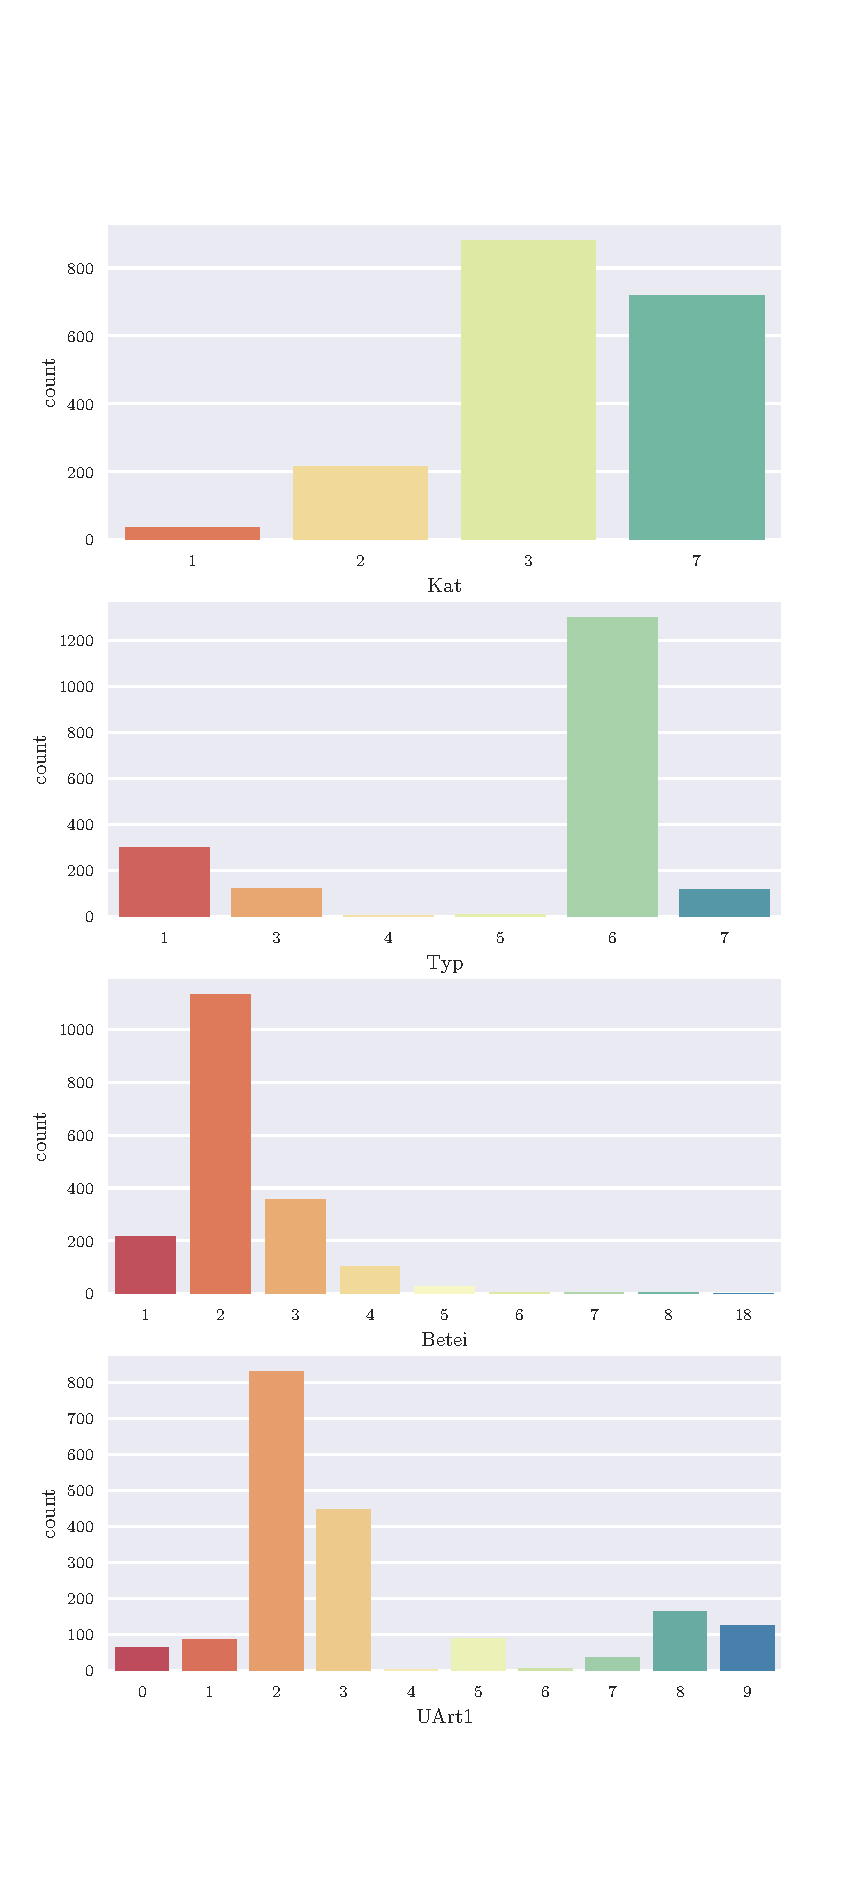
\includegraphics[scale=0.7]{CorrAnalysis/data/BAYSIS/02_matched/plots/baysis_matched_count_multiple01}
    %     \caption{Distribution of the accident category Kat, Typ, Betei and UArt}
    %     \label{img:baysis_matched_Kat}
    %     \label{img:baysis_matched_Typ}
    %     \label{img:baysis_matched_Betei}
    %     \label{img:baysis_matched_UArt}
    % \end{figure}

    % \begin{figure}[ht!]
    %     \centering
    %     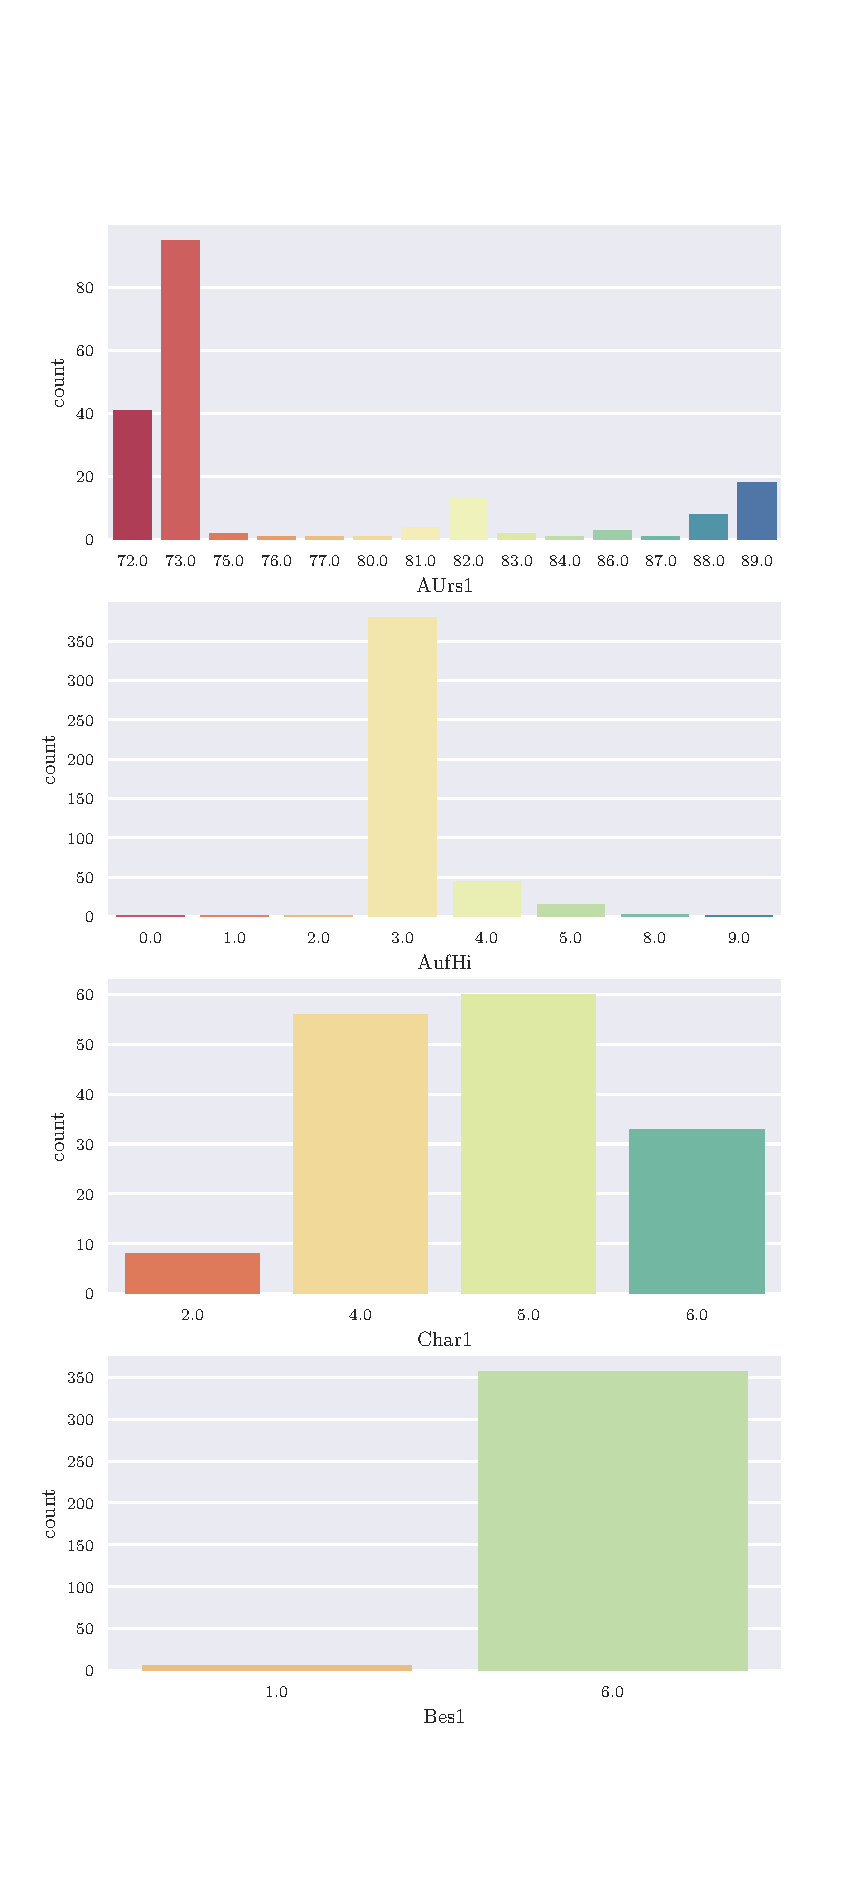
\includegraphics[scale=0.7]{CorrAnalysis/data/BAYSIS/02_matched/plots/baysis_matched_count_multiple02}
    %     \caption{Distribution of the accident category AUrs, AufHi, Char and Bes}
    %     \label{img:baysis_matched_AUrs}
    %     \label{img:baysis_matched_AufHi}
    %     \label{img:baysis_matched_Char}
    %     \label{img:baysis_matched_Bes}
    % \end{figure}

    % \begin{figure}[ht!]
    %     \centering
    %     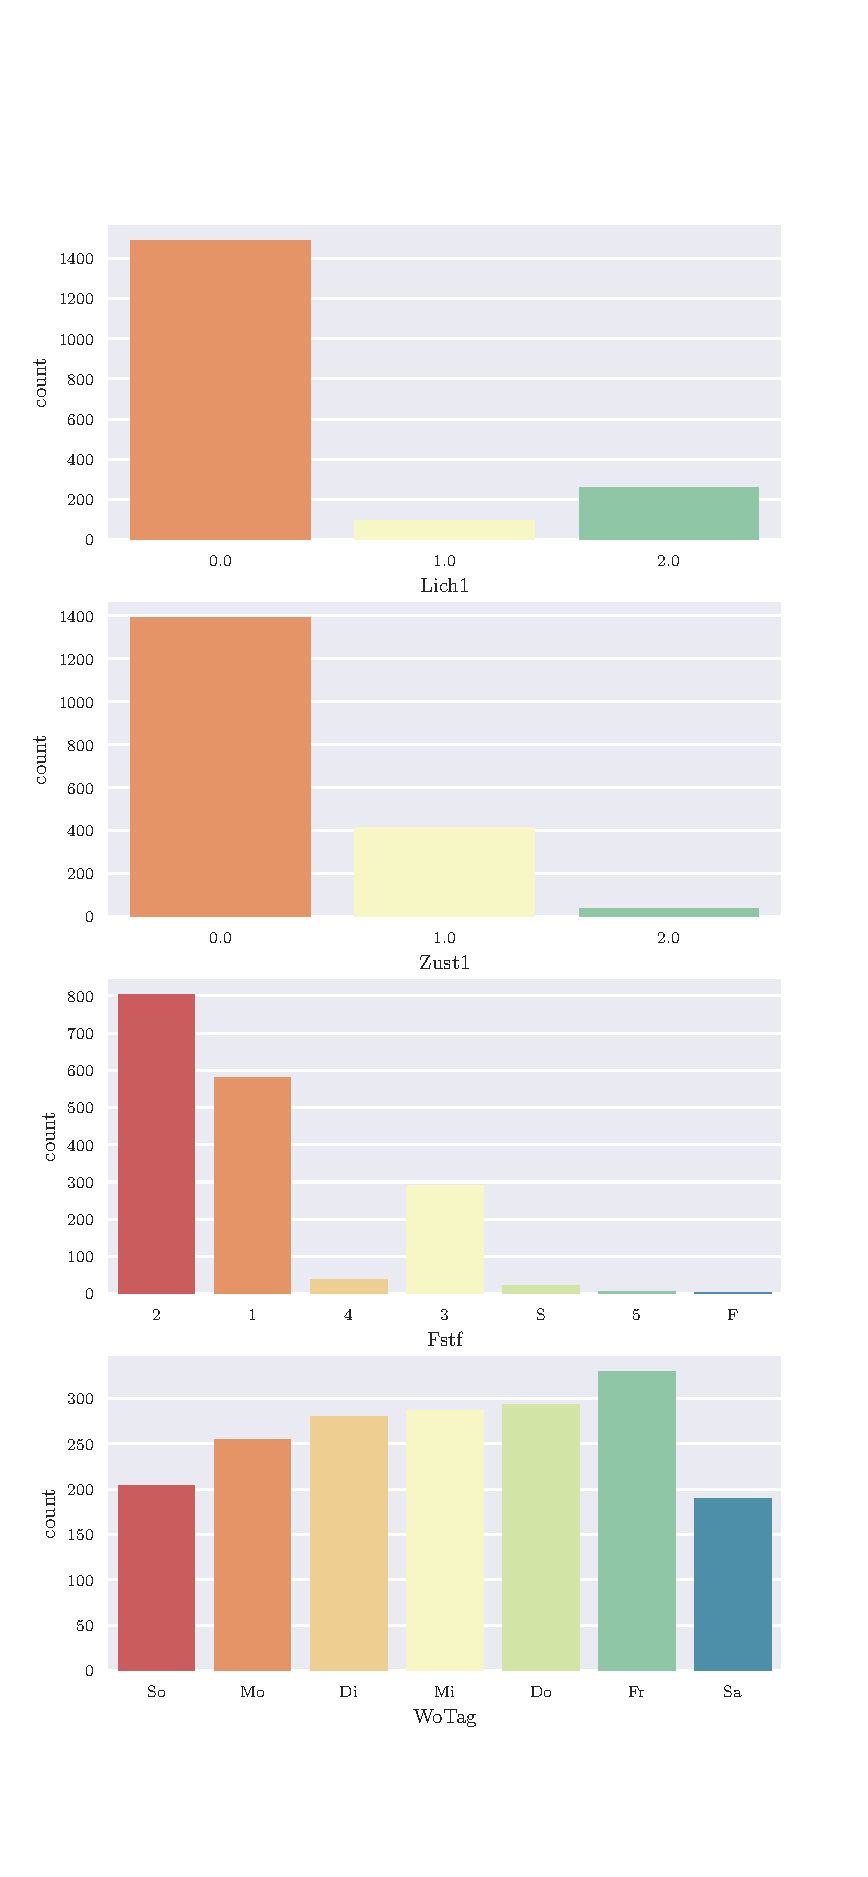
\includegraphics[scale=0.7]{CorrAnalysis/data/BAYSIS/02_matched/plots/baysis_matched_count_multiple03}
    %     \caption{Distribution of the accident category Lich, Zust, Fstf and WoTag}
    %     \label{img:baysis_matched_Lich}
    %     \label{img:baysis_matched_Zust}
    %     \label{img:baysis_matched_Fstf}
    %     \label{img:baysis_matched_WoTag}
    % \end{figure}

    \begin{table}[ht!]
        \tiny
        \centering
        \begin{tabular}{rrrrrr}
            \toprule
            & 1 & 3 & 4 & 5 & 6 \\ 
            \midrule
            3 & \red{0.05} &  &  &  &  \\ 
            4 & 1.00 & 0.38 &  &  &  \\ 
            5 & 0.96 & 1.00 & 0.96 &  &  \\ 
            6 & \red{0.00} & 0.96 & 0.51 & 1.00 &  \\ 
            7 & 1.00 & \red{0.04} & 1.00 & 0.96 & \red{0.01} \\ 
            \bottomrule
        \end{tabular}
        \caption{Pairwise Wilcoxon $T$-test for \textit{Typ} and \textit{Temporal Distance} (Jam Initiator) complete}
        \label{tbl:wilcoxon_baysis_initiator_Typ_TDist_complete}
    \end{table}

    \begin{table}[ht!]
        \tiny
        \centering
        \begin{tabular}{rrrrrrrrrr}
            \toprule
            & 0 & 1 & 2 & 3 & 4 & 5 & 6 & 7 & 8 \\ 
            \midrule
            1 & 1.00 &  &  &  &  &  &  &  &  \\ 
            2 & 1.00 & 1.00 &  &  &  &  &  &  &  \\ 
            3 & 1.00 & \red{0.04} & 0.00 &  &  &  &  &  &  \\ 
            4 & 1.00 & 1.00 & 1.00 & 1.00 &  &  &  &  &  \\ 
            5 & 1.00 & 1.00 & 1.00 & 1.00 & 1.00 &  &  &  &  \\ 
            6 & 1.00 & 1.00 & 1.00 & 1.00 & 1.00 & 1.00 &  &  &  \\ 
            7 & 0.75 & 0.05 & 0.13 & 1.00 & 1.00 & 1.00 & 1.00 &  &  \\ 
            8 & 1.00 & 0.21 & 0.47 & 1.00 & 1.00 & 1.00 & 1.00 & 1.00 &  \\ 
            9 & 1.00 & 0.45 & 1.00 & 1.00 & 1.00 & 1.00 & 1.00 & 1.00 & 1.00 \\ 
            \bottomrule
          \end{tabular}
        \caption{Pairwise Wilcoxon $T$-test for \textit{UArt1} and \textit{Maximal Temporal Extent} (Jam Initiator)}
        \label{tbl:wilcoxon_baysis_initiator_UArt1_TMax}
    \end{table}

    \begin{table}[ht!]
        \tiny
        \centering
        \begin{tabular}{rrrrrrrrrr}
            \toprule
              & 0 & 1 & 2 & 3 & 4 & 5 & 6 & 7 & 8 \\ 
            \midrule
            1 & 1.00 &  &  &  &  &  &  &  &  \\ 
            2 & 1.00 & 1.00 &  &  &  &  &  &  &  \\ 
            3 & 1.00 & 1.00 & 1.00 &  &  &  &  &  &  \\ 
            4 & 1.00 & 1.00 & 1.00 & 1.00 &  &  &  &  &  \\ 
            5 & 1.00 & 1.00 & 1.00 & 1.00 & 1.00 &  &  &  &  \\ 
            6 & 1.00 & 1.00 & 1.00 & 1.00 & 1.00 & 1.00 &  &  &  \\ 
            7 & 1.00 & 0.06 & \red{0.00} & \red{0.00} & 1.00 & 0.10 & 1.00 &  &  \\ 
            8 & 1.00 & 1.00 & \red{0.01} & \red{0.01} & 1.00 & 1.00 & 1.00 & 1.00 &  \\ 
            9 & 1.00 & 1.00 & \red{0.05} & \red{0.01} & 1.00 & 0.78 & 1.00 & 0.87 & 1.00 \\ 
            \bottomrule
          \end{tabular}
        \caption{Pairwise Wilcoxon $T$-test for \textit{UArt1} and \textit{Temporal Distance} (Jam Initiator) complete}
        \label{tbl:wilcoxon_baysis_initiator_UArt1_TDist_complete}
    \end{table}

    \begin{table}[ht!]
        \tiny
        \centering
        \begin{tabular}{rrrrrrrrrr}
            \toprule
              & 0 & 1 & 2 & 3 & 4 & 5 & 6 & 7 & 8 \\ 
            \midrule
            1 & 1.00 &  &  &  &  &  &  &  &  \\ 
            2 & 1.00 & 1.00 &  &  &  &  &  &  &  \\ 
            3 & 1.00 & 1.00 & 1.00 &  &  &  &  &  &  \\ 
            4 & 1.00 & 1.00 & 1.00 & 1.00 &  &  &  &  &  \\ 
            5 & 1.00 & 1.00 & 1.00 & 1.00 & 1.00 &  &  &  &  \\ 
            6 & 1.00 & 1.00 & 1.00 & 1.00 & 1.00 & 1.00 &  &  &  \\ 
            7 & 1.00 & 1.00 & 1.00 & 1.00 & 1.00 & 1.00 & 1.00 &  &  \\ 
            8 & 1.00 & 1.00 & 0.13 & 0.09 & 1.00 & 0.72 & 1.00 & 1.00 &  \\ 
            9 & 1.00 & 1.00 & 1.00 & 1.00 & 1.00 & 1.00 & 1.00 & 1.00 & 1.00 \\ 
            \bottomrule
          \end{tabular}
        \caption{Pairwise Wilcoxon $T$-test for \textit{UArt1} and \textit{Coverage} (Jam Initiator)}
        \label{tbl:wilcoxon_baysis_initiator_UArt1_Cov}
    \end{table}
    
    % ------- BAYSIS Selected01 - Tables --------
    % \newgeometry{left=1cm,right=1cm,bottom=2cm}
    \begin{sidewaystable}
    	\tiny
    	\setlength{\tabcolsep}{2pt}
    	\centering
    	\begin{tabular}{lrrrrrrrrrrrrrrrrrrrrrrrrrrrrr}
\toprule
{} &  TMax &  TAvg &  SMax &  SAvg &  TDist &  SDist &   Cov &  TLCar &  TLHGV &  Str &  Kat &  Typ &  Betei &  UArt1 &  UArt2 &  AUrs1 &  AUrs2 &  AufHi &  Alkoh &  Char1 &  Char2 &  Lich1 &  Lich2 &  Zust1 &  Zust2 &  Fstf &  WoTag &  FeiTag &  Month \\
\midrule
TMax   &  1.00 &  0.89 &  0.60 &  0.53 &  -0.11 &  -0.03 & -0.21 &   0.02 &  -0.00 & 0.18 & 0.29 & 0.06 &   0.14 &   0.16 &   0.05 &   0.23 &   0.15 &   0.16 &   0.00 &   0.05 &   0.04 &   0.02 &   0.02 &   0.10 &   0.10 &  0.03 &   0.07 &   -0.02 &   0.12 \\
TAvg   &  0.89 &  1.00 &  0.39 &  0.55 &  -0.09 &  -0.03 &  0.08 &   0.01 &  -0.01 & 0.15 & 0.27 & 0.11 &   0.09 &   0.20 &   0.07 &   0.21 &   0.20 &   0.14 &   0.02 &   0.04 &   0.04 &   0.04 &   0.01 &   0.08 &   0.16 &  0.03 &   0.10 &   -0.01 &   0.11 \\
SMax   &  0.60 &  0.39 &  1.00 &  0.72 &  -0.09 &  -0.01 & -0.46 &   0.02 &  -0.00 & 0.26 & 0.20 & 0.08 &   0.11 &   0.20 &   0.07 &   0.22 &   0.11 &   0.13 &  -0.06 &   0.09 &   0.06 &   0.13 &   0.08 &   0.10 &   0.07 &  0.03 &   0.08 &   -0.02 &   0.14 \\
SAvg   &  0.53 &  0.55 &  0.72 &  1.00 &  -0.01 &  -0.04 &  0.10 &   0.05 &  -0.04 & 0.24 & 0.26 & 0.16 &   0.08 &   0.27 &   0.06 &   0.25 &   0.19 &   0.09 &  -0.03 &   0.07 &   0.02 &   0.03 &   0.02 &   0.09 &   0.16 &  0.04 &   0.12 &    0.00 &   0.13 \\
TDist  & -0.11 & -0.09 & -0.09 & -0.01 &   1.00 &   0.03 &  0.13 &  -0.01 &   0.06 & 0.10 & 0.10 & 0.21 &  -0.13 &   0.24 &   0.03 &   0.22 &   0.15 &   0.14 &   0.07 &   0.14 &   0.12 &   0.18 &   0.17 &   0.13 &   0.01 &  0.05 &   0.10 &    0.00 &   0.11 \\
SDist  & -0.03 & -0.03 & -0.01 & -0.04 &   0.03 &   1.00 & -0.07 &  -0.00 &  -0.00 & 0.06 & 0.07 & 0.03 &  -0.02 &   0.07 &   0.02 &   0.02 &   0.00 &   0.03 &  -0.00 &   0.01 &   0.01 &   0.02 &   0.02 &   0.02 &   0.00 &  0.07 &   0.09 &   -0.01 &   0.11 \\
Cov    & -0.21 &  0.08 & -0.46 &  0.10 &   0.13 &  -0.07 &  1.00 &   0.02 &  -0.04 & 0.22 & 0.04 & 0.18 &  -0.07 &   0.19 &   0.06 &   0.25 &   0.13 &   0.14 &   0.08 &   0.11 &   0.07 &   0.12 &   0.09 &   0.18 &   0.04 &  0.03 &   0.13 &    0.03 &   0.16 \\
TLCar  &  0.02 &  0.01 &  0.02 &  0.05 &  -0.01 &  -0.00 &  0.02 &   1.00 &   0.02 & 0.18 & 0.03 & 0.10 &   0.02 &   0.15 &   0.10 &   0.12 &   0.09 &   0.07 &   0.01 &   0.08 &   0.04 &   0.04 &   0.04 &   0.06 &   0.01 &  0.03 &   0.07 &    0.03 &   0.09 \\
TLHGV  & -0.00 & -0.01 & -0.00 & -0.04 &   0.06 &  -0.00 & -0.04 &   0.02 &   1.00 & 0.13 & 0.09 & 0.08 &  -0.03 &   0.09 &   0.07 &   0.18 &   0.11 &   0.08 &   0.07 &   0.10 &   0.03 &   0.06 &   0.06 &   0.03 &   0.05 &  0.02 &   0.13 &    0.01 &   0.16 \\
Str    &  0.18 &  0.15 &  0.26 &  0.24 &   0.10 &   0.06 &  0.22 &   0.18 &   0.13 & 1.00 & 0.16 & 0.16 &   0.13 &   0.13 &   0.16 &   0.13 &   0.08 &   0.13 &   0.07 &   0.14 &   0.12 &   0.12 &   0.16 &   0.11 &   0.15 &  0.19 &   0.15 &    0.07 &   0.15 \\
Kat    &  0.29 &  0.27 &  0.20 &  0.26 &   0.10 &   0.07 &  0.04 &   0.03 &   0.09 & 0.16 & 1.00 & 0.20 &   0.17 &   0.31 &   0.14 &   0.18 &   0.09 &   0.20 &   0.05 &   0.13 &   0.10 &   0.09 &   0.10 &   0.12 &   0.09 &  0.11 &   0.09 &    0.03 &   0.14 \\
Typ    &  0.06 &  0.11 &  0.08 &  0.16 &   0.21 &   0.03 &  0.18 &   0.10 &   0.08 & 0.16 & 0.20 & 1.00 &   0.30 &   0.63 &   0.09 &   0.25 &   0.10 &   0.24 &   0.16 &   0.15 &   0.20 &   0.08 &   0.08 &   0.19 &   0.08 &  0.13 &   0.11 &    0.04 &   0.13 \\
Betei  &  0.14 &  0.09 &  0.11 &  0.08 &  -0.13 &  -0.02 & -0.07 &   0.02 &  -0.03 & 0.13 & 0.17 & 0.30 &   1.00 &   0.29 &   0.10 &   0.21 &   0.42 &   0.19 &   0.05 &   0.11 &   0.18 &   0.10 &   0.09 &   0.12 &   0.42 &  0.10 &   0.11 &    0.04 &   0.13 \\
UArt1  &  0.16 &  0.20 &  0.20 &  0.27 &   0.24 &   0.07 &  0.19 &   0.15 &   0.09 & 0.13 & 0.31 & 0.63 &   0.29 &   1.00 &   0.16 &   0.21 &   0.11 &   0.29 &   0.16 &   0.22 &   0.19 &   0.11 &   0.12 &   0.19 &   0.09 &  0.15 &   0.14 &    0.08 &   0.12 \\
UArt2  &  0.05 &  0.07 &  0.07 &  0.06 &   0.03 &   0.02 &  0.06 &   0.10 &   0.07 & 0.16 & 0.14 & 0.09 &   0.10 &   0.16 &   1.00 &   0.14 &   0.07 &   0.26 &   0.03 &   0.11 &   0.13 &   0.09 &   0.11 &   0.08 &   0.03 &  0.12 &   0.10 &    0.07 &   0.14 \\
AUrs1  &  0.23 &  0.21 &  0.22 &  0.25 &   0.22 &   0.02 &  0.25 &   0.12 &   0.18 & 0.13 & 0.18 & 0.25 &   0.21 &   0.21 &   0.14 &   1.00 &   0.45 &   0.13 &   0.05 &   0.15 &   0.20 &   0.11 &   0.11 &   0.49 &   0.59 &  0.08 &   0.12 &    0.06 &   0.16 \\
AUrs2  &  0.15 &  0.20 &  0.11 &  0.19 &   0.15 &   0.00 &  0.13 &   0.09 &   0.11 & 0.08 & 0.09 & 0.10 &   0.42 &   0.11 &   0.07 &   0.45 &   1.00 &   0.05 &   0.01 &   0.06 &   0.13 &   0.04 &   0.04 &   0.18 &   0.65 &  0.05 &   0.10 &    0.02 &   0.12 \\
AufHi  &  0.16 &  0.14 &  0.13 &  0.09 &   0.14 &   0.03 &  0.14 &   0.07 &   0.08 & 0.13 & 0.20 & 0.24 &   0.19 &   0.29 &   0.26 &   0.13 &   0.05 &   1.00 &   0.03 &   0.12 &   0.18 &   0.08 &   0.09 &   0.15 &   0.03 &  0.12 &   0.11 &    0.05 &   0.12 \\
Alkoh  &  0.00 &  0.02 & -0.06 & -0.03 &   0.07 &  -0.00 &  0.08 &   0.01 &   0.07 & 0.07 & 0.05 & 0.16 &   0.05 &   0.16 &   0.03 &   0.05 &   0.01 &   0.03 &   1.00 &   0.08 &   0.01 &   0.17 &   0.14 &   0.02 &   0.05 &  0.10 &   0.04 &    0.01 &   0.10 \\
Char1  &  0.05 &  0.04 &  0.09 &  0.07 &   0.14 &   0.01 &  0.11 &   0.08 &   0.10 & 0.14 & 0.13 & 0.15 &   0.11 &   0.22 &   0.11 &   0.15 &   0.06 &   0.12 &   0.08 &   1.00 &   0.62 &   0.07 &   0.09 &   0.10 &   0.04 &  0.08 &   0.09 &    0.06 &   0.12 \\
Char2  &  0.04 &  0.04 &  0.06 &  0.02 &   0.12 &   0.01 &  0.07 &   0.04 &   0.03 & 0.12 & 0.10 & 0.20 &   0.18 &   0.19 &   0.13 &   0.20 &   0.13 &   0.18 &   0.01 &   0.62 &   1.00 &   0.08 &   0.08 &   0.16 &   0.02 &  0.13 &   0.15 &    0.06 &   0.07 \\
Lich1  &  0.02 &  0.04 &  0.13 &  0.03 &   0.18 &   0.02 &  0.12 &   0.04 &   0.06 & 0.12 & 0.09 & 0.08 &   0.10 &   0.11 &   0.09 &   0.11 &   0.04 &   0.08 &   0.17 &   0.07 &   0.08 &   1.00 &   0.71 &   0.43 &   0.05 &  0.08 &   0.11 &    0.06 &   0.20 \\
Lich2  &  0.02 &  0.01 &  0.08 &  0.02 &   0.17 &   0.02 &  0.09 &   0.04 &   0.06 & 0.16 & 0.10 & 0.08 &   0.09 &   0.12 &   0.11 &   0.11 &   0.04 &   0.09 &   0.14 &   0.09 &   0.08 &   0.71 &   1.00 &   0.15 &   0.02 &  0.06 &   0.14 &    0.07 &   0.23 \\
Zust1  &  0.10 &  0.08 &  0.10 &  0.09 &   0.13 &   0.02 &  0.18 &   0.06 &   0.03 & 0.11 & 0.12 & 0.19 &   0.12 &   0.19 &   0.08 &   0.49 &   0.18 &   0.15 &   0.02 &   0.10 &   0.16 &   0.43 &   0.15 &   1.00 &   0.16 &  0.09 &   0.09 &    0.05 &   0.27 \\
Zust2  &  0.10 &  0.16 &  0.07 &  0.16 &   0.01 &   0.00 &  0.04 &   0.01 &   0.05 & 0.15 & 0.09 & 0.08 &   0.42 &   0.09 &   0.03 &   0.59 &   0.65 &   0.03 &   0.05 &   0.04 &   0.02 &   0.05 &   0.02 &   0.16 &   1.00 &  0.04 &   0.10 &    0.02 &   0.20 \\
Fstf   &  0.03 &  0.03 &  0.03 &  0.04 &   0.05 &   0.07 &  0.03 &   0.03 &   0.02 & 0.19 & 0.11 & 0.13 &   0.10 &   0.15 &   0.12 &   0.08 &   0.05 &   0.12 &   0.10 &   0.08 &   0.13 &   0.08 &   0.06 &   0.09 &   0.04 &  1.00 &   0.10 &    0.06 &   0.13 \\
WoTag  &  0.07 &  0.10 &  0.08 &  0.12 &   0.10 &   0.09 &  0.13 &   0.07 &   0.13 & 0.15 & 0.09 & 0.11 &   0.11 &   0.14 &   0.10 &   0.12 &   0.10 &   0.11 &   0.04 &   0.09 &   0.15 &   0.11 &   0.14 &   0.09 &   0.10 &  0.10 &   1.00 &    0.18 &   0.15 \\
FeiTag & -0.02 & -0.01 & -0.02 &  0.00 &   0.00 &  -0.01 &  0.03 &   0.03 &   0.01 & 0.07 & 0.03 & 0.04 &   0.04 &   0.08 &   0.07 &   0.06 &   0.02 &   0.05 &   0.01 &   0.06 &   0.06 &   0.06 &   0.07 &   0.05 &   0.02 &  0.06 &   0.18 &    1.00 &   0.21 \\
Month  &  0.12 &  0.11 &  0.14 &  0.13 &   0.11 &   0.11 &  0.16 &   0.09 &   0.16 & 0.15 & 0.14 & 0.13 &   0.13 &   0.12 &   0.14 &   0.16 &   0.12 &   0.12 &   0.10 &   0.12 &   0.07 &   0.20 &   0.23 &   0.27 &   0.20 &  0.13 &   0.15 &    0.21 &   1.00 \\
\bottomrule
\end{tabular}

    	\caption{Correlation matrix for BAYSIS selected data (Jam Initiator), calculated with Cramer's $V$, $\eta$, $\tau$, $r_{pq}$, $r$}
    	\label{table:appendix_correlation_matrix_selected_startJam_cramers}
    \end{sidewaystable}
    \begin{sidewaystable}
    	\tiny
    	\setlength{\tabcolsep}{2pt}
    	\centering
    	\begin{tabular}{lrrrrrrrrrrrrrrrrrrrrrrrrrrrrr}
\toprule
{} &  TMax &  TAvg &  SMax &  SAvg &  TDist &  SDist &   Cov &  TLCar &  TLHGV &  Str &  Kat &  Typ &  Betei &  UArt1 &  UArt2 &  AUrs1 &  AUrs2 &  AufHi &  Alkoh &  Char1 &  Char2 &  Lich1 &  Lich2 &  Zust1 &  Zust2 &  Fstf &  WoTag &  FeiTag &  Month \\
\midrule
TMax   &  1.00 &  0.89 &  0.60 &  0.53 &  -0.11 &  -0.03 & -0.21 &   0.02 &  -0.00 & 0.18 & 0.29 & 0.06 &   0.14 &   0.16 &   0.05 &   0.23 &   0.15 &   0.16 &   0.00 &   0.05 &   0.04 &   0.02 &   0.02 &   0.10 &   0.10 &  0.03 &   0.07 &   -0.02 &   0.12 \\
TAvg   &  0.89 &  1.00 &  0.39 &  0.55 &  -0.09 &  -0.03 &  0.08 &   0.01 &  -0.01 & 0.15 & 0.27 & 0.11 &   0.09 &   0.20 &   0.07 &   0.21 &   0.20 &   0.14 &   0.02 &   0.04 &   0.04 &   0.04 &   0.01 &   0.08 &   0.16 &  0.03 &   0.10 &   -0.01 &   0.11 \\
SMax   &  0.60 &  0.39 &  1.00 &  0.72 &  -0.09 &  -0.01 & -0.46 &   0.02 &  -0.00 & 0.26 & 0.20 & 0.08 &   0.11 &   0.20 &   0.07 &   0.22 &   0.11 &   0.13 &  -0.06 &   0.09 &   0.06 &   0.13 &   0.08 &   0.10 &   0.07 &  0.03 &   0.08 &   -0.02 &   0.14 \\
SAvg   &  0.53 &  0.55 &  0.72 &  1.00 &  -0.01 &  -0.04 &  0.10 &   0.05 &  -0.04 & 0.24 & 0.26 & 0.16 &   0.08 &   0.27 &   0.06 &   0.25 &   0.19 &   0.09 &  -0.03 &   0.07 &   0.02 &   0.03 &   0.02 &   0.09 &   0.16 &  0.04 &   0.12 &    0.00 &   0.13 \\
TDist  & -0.11 & -0.09 & -0.09 & -0.01 &   1.00 &   0.03 &  0.13 &  -0.01 &   0.06 & 0.10 & 0.10 & 0.21 &  -0.13 &   0.24 &   0.03 &   0.22 &   0.15 &   0.14 &   0.07 &   0.14 &   0.12 &   0.18 &   0.17 &   0.13 &   0.01 &  0.05 &   0.10 &    0.00 &   0.11 \\
SDist  & -0.03 & -0.03 & -0.01 & -0.04 &   0.03 &   1.00 & -0.07 &  -0.00 &  -0.00 & 0.06 & 0.07 & 0.03 &  -0.02 &   0.07 &   0.02 &   0.02 &   0.00 &   0.03 &  -0.00 &   0.01 &   0.01 &   0.02 &   0.02 &   0.02 &   0.00 &  0.07 &   0.09 &   -0.01 &   0.11 \\
Cov    & -0.21 &  0.08 & -0.46 &  0.10 &   0.13 &  -0.07 &  1.00 &   0.02 &  -0.04 & 0.22 & 0.04 & 0.18 &  -0.07 &   0.19 &   0.06 &   0.25 &   0.13 &   0.14 &   0.08 &   0.11 &   0.07 &   0.12 &   0.09 &   0.18 &   0.04 &  0.03 &   0.13 &    0.03 &   0.16 \\
TLCar  &  0.02 &  0.01 &  0.02 &  0.05 &  -0.01 &  -0.00 &  0.02 &   1.00 &   0.02 & 0.18 & 0.03 & 0.10 &   0.02 &   0.15 &   0.10 &   0.12 &   0.09 &   0.07 &   0.01 &   0.08 &   0.04 &   0.04 &   0.04 &   0.06 &   0.01 &  0.03 &   0.07 &    0.03 &   0.09 \\
TLHGV  & -0.00 & -0.01 & -0.00 & -0.04 &   0.06 &  -0.00 & -0.04 &   0.02 &   1.00 & 0.13 & 0.09 & 0.08 &  -0.03 &   0.09 &   0.07 &   0.18 &   0.11 &   0.08 &   0.07 &   0.10 &   0.03 &   0.06 &   0.06 &   0.03 &   0.05 &  0.02 &   0.13 &    0.01 &   0.16 \\
Str    &  0.18 &  0.15 &  0.26 &  0.24 &   0.10 &   0.06 &  0.22 &   0.18 &   0.13 & 1.00 & 0.02 & 0.03 &   0.03 &   0.03 &   0.03 &   0.03 &   0.01 &   0.02 &   0.00 &   0.02 &   0.00 &   0.01 &   0.01 &   0.01 &   0.00 &  0.06 &   0.03 &    0.00 &   0.05 \\
Kat    &  0.29 &  0.27 &  0.20 &  0.26 &   0.10 &   0.07 &  0.04 &   0.03 &   0.09 & 0.04 & 1.00 & 0.05 &   0.04 &   0.10 &   0.02 &   0.04 &   0.01 &   0.04 &   0.00 &   0.02 &   0.00 &   0.01 &   0.01 &   0.02 &   0.00 &  0.02 &   0.01 &    0.00 &   0.03 \\
Typ    &  0.06 &  0.11 &  0.08 &  0.16 &   0.21 &   0.03 &  0.18 &   0.10 &   0.08 & 0.06 & 0.05 & 1.00 &   0.22 &   0.37 &   0.02 &   0.12 &   0.02 &   0.15 &   0.01 &   0.03 &   0.02 &   0.01 &   0.01 &   0.05 &   0.00 &  0.03 &   0.03 &    0.00 &   0.04 \\
Betei  &  0.14 &  0.09 &  0.11 &  0.08 &  -0.13 &  -0.02 & -0.07 &   0.02 &  -0.03 & 0.05 & 0.03 & 0.16 &   1.00 &   0.23 &   0.02 &   0.07 &   0.02 &   0.11 &   0.00 &   0.02 &   0.01 &   0.01 &   0.01 &   0.02 &   0.01 &  0.02 &   0.03 &    0.00 &   0.04 \\
UArt1  &  0.16 &  0.20 &  0.20 &  0.27 &   0.24 &   0.07 &  0.19 &   0.15 &   0.09 & 0.04 & 0.07 & 0.22 &   0.18 &   1.00 &   0.05 &   0.07 &   0.01 &   0.22 &   0.00 &   0.03 &   0.01 &   0.01 &   0.01 &   0.03 &   0.00 &  0.04 &   0.04 &    0.00 &   0.04 \\
UArt2  &  0.05 &  0.07 &  0.07 &  0.06 &   0.03 &   0.02 &  0.06 &   0.10 &   0.07 & 0.07 & 0.03 & 0.03 &   0.04 &   0.11 &   1.00 &   0.04 &   0.01 &   0.30 &   0.00 &   0.02 &   0.01 &   0.01 &   0.01 &   0.01 &   0.00 &  0.05 &   0.04 &    0.00 &   0.08 \\
AUrs1  &  0.23 &  0.21 &  0.22 &  0.25 &   0.22 &   0.02 &  0.25 &   0.12 &   0.18 & 0.11 & 0.07 & 0.18 &   0.14 &   0.17 &   0.04 &   1.00 &   0.06 &   0.11 &   0.00 &   0.04 &   0.02 &   0.03 &   0.02 &   0.31 &   0.05 &  0.04 &   0.07 &    0.00 &   0.16 \\
AUrs2  &  0.15 &  0.20 &  0.11 &  0.19 &   0.15 &   0.00 &  0.13 &   0.09 &   0.11 & 0.19 & 0.13 & 0.22 &   0.30 &   0.23 &   0.12 &   0.52 &   1.00 &   0.11 &   0.00 &   0.04 &   0.04 &   0.04 &   0.04 &   0.23 &   0.26 &  0.12 &   0.26 &    0.00 &   0.30 \\
AufHi  &  0.16 &  0.14 &  0.13 &  0.09 &   0.14 &   0.03 &  0.14 &   0.07 &   0.08 & 0.06 & 0.04 & 0.17 &   0.16 &   0.41 &   0.27 &   0.08 &   0.01 &   1.00 &   0.00 &   0.03 &   0.02 &   0.01 &   0.01 &   0.04 &   0.00 &  0.04 &   0.05 &    0.00 &   0.06 \\
Alkoh  &  0.00 &  0.02 & -0.06 & -0.03 &   0.07 &  -0.00 &  0.08 &   0.01 &   0.07 & 0.04 & 0.02 & 0.07 &   0.03 &   0.09 &   0.01 &   0.02 &   0.00 &   0.01 &   1.00 &   0.04 &   0.01 &   0.14 &   0.10 &   0.01 &   0.00 &  0.08 &   0.01 &    0.01 &   0.09 \\
Char1  &  0.05 &  0.04 &  0.09 &  0.07 &   0.14 &   0.01 &  0.11 &   0.08 &   0.10 & 0.08 & 0.05 & 0.06 &   0.04 &   0.08 &   0.03 &   0.05 &   0.01 &   0.04 &   0.01 &   1.00 &   0.19 &   0.01 &   0.01 &   0.03 &   0.00 &  0.03 &   0.03 &    0.00 &   0.05 \\
Char2  &  0.04 &  0.04 &  0.06 &  0.02 &   0.12 &   0.01 &  0.07 &   0.04 &   0.03 & 0.06 & 0.03 & 0.10 &   0.07 &   0.10 &   0.04 &   0.08 &   0.02 &   0.09 &   0.00 &   0.61 &   1.00 &   0.02 &   0.02 &   0.06 &   0.00 &  0.05 &   0.06 &    0.01 &   0.02 \\
Lich1  &  0.02 &  0.04 &  0.13 &  0.03 &   0.18 &   0.02 &  0.12 &   0.04 &   0.06 & 0.03 & 0.01 & 0.01 &   0.02 &   0.02 &   0.02 &   0.02 &   0.00 &   0.02 &   0.01 &   0.01 &   0.00 &   1.00 &   0.79 &   0.05 &   0.00 &  0.01 &   0.02 &    0.00 &   0.07 \\
Lich2  &  0.02 &  0.01 &  0.08 &  0.02 &   0.17 &   0.02 &  0.09 &   0.04 &   0.06 & 0.04 & 0.02 & 0.01 &   0.02 &   0.02 &   0.02 &   0.02 &   0.00 &   0.01 &   0.01 &   0.01 &   0.01 &   0.94 &   1.00 &   0.04 &   0.00 &  0.01 &   0.03 &    0.00 &   0.08 \\
Zust1  &  0.10 &  0.08 &  0.10 &  0.09 &   0.13 &   0.02 &  0.18 &   0.06 &   0.03 & 0.03 & 0.03 & 0.07 &   0.03 &   0.06 &   0.01 &   0.28 &   0.02 &   0.05 &   0.00 &   0.02 &   0.01 &   0.05 &   0.03 &   1.00 &   0.02 &  0.02 &   0.02 &    0.00 &   0.10 \\
Zust2  &  0.10 &  0.16 &  0.07 &  0.16 &   0.01 &   0.00 &  0.04 &   0.01 &   0.05 & 0.17 & 0.08 & 0.06 &   0.24 &   0.07 &   0.02 &   0.68 &   0.37 &   0.01 &   0.00 &   0.02 &   0.01 &   0.04 &   0.01 &   0.23 &   1.00 &  0.02 &   0.09 &    0.01 &   0.28 \\
Fstf   &  0.03 &  0.03 &  0.03 &  0.04 &   0.05 &   0.07 &  0.03 &   0.03 &   0.02 & 0.09 & 0.01 & 0.03 &   0.02 &   0.05 &   0.03 &   0.02 &   0.01 &   0.02 &   0.00 &   0.01 &   0.01 &   0.01 &   0.00 &   0.01 &   0.00 &  1.00 &   0.02 &    0.00 &   0.04 \\
WoTag  &  0.07 &  0.10 &  0.08 &  0.12 &   0.10 &   0.09 &  0.13 &   0.07 &   0.13 & 0.04 & 0.01 & 0.02 &   0.02 &   0.03 &   0.02 &   0.02 &   0.01 &   0.02 &   0.00 &   0.01 &   0.01 &   0.01 &   0.01 &   0.01 &   0.00 &  0.01 &   1.00 &    0.01 &   0.03 \\
FeiTag & -0.02 & -0.01 & -0.02 &  0.00 &   0.00 &  -0.01 &  0.03 &   0.03 &   0.01 & 0.03 & 0.00 & 0.01 &   0.01 &   0.04 &   0.02 &   0.02 &   0.00 &   0.01 &   0.00 &   0.01 &   0.02 &   0.01 &   0.01 &   0.01 &   0.00 &  0.02 &   0.12 &    1.00 &   0.17 \\
Month  &  0.12 &  0.11 &  0.14 &  0.13 &   0.11 &   0.11 &  0.16 &   0.09 &   0.16 & 0.04 & 0.01 & 0.02 &   0.02 &   0.03 &   0.03 &   0.04 &   0.01 &   0.02 &   0.00 &   0.01 &   0.00 &   0.02 &   0.02 &   0.03 &   0.01 &  0.02 &   0.03 &    0.01 &   1.00 \\
\bottomrule
\end{tabular}

    	\caption{Correlation matrix for BAYSIS selected data (Jam Initiator), calculated with Theil's $U$, $\eta$, $\tau$, $r_{pq}$, $r$}
    	\label{table:appendix_correlation_matrix_selected_startJam_theils}
    \end{sidewaystable}
    \begin{sidewaystable}
    	\tiny
    	\setlength{\tabcolsep}{2pt}
    	\centering
    	\begin{tabular}{lrrrrrrrrrrrrrrrrrrrrrrrrrrrrr}
\toprule
{} &  TMax &  TAvg &  SMax &  SAvg &  TDist &  SDist &   Cov &  TLCar &  TLHGV &   Str &   Kat &   Typ &  Betei &  UArt1 &  UArt2 &  AUrs1 &  AUrs2 &  AufHi &  Alkoh &  Char1 &  Char2 &  Lich1 &  Lich2 &  Zust1 &  Zust2 &  Fstf &  WoTag &  FeiTag &  Month \\
\midrule
TMax   &   nan & 0.000 & 0.000 & 0.000 &  0.002 &  0.361 & 0.000 &  0.671 &  0.921 & 0.000 & 0.000 & 0.000 &  0.000 &  0.000 &  0.000 &  0.000 &  0.000 &  0.000 &  0.965 &  0.000 &  0.000 &  0.000 &  0.000 &  0.000 &  0.000 & 0.325 &  0.000 &   0.576 &  0.000 \\
TAvg   & 0.000 &   nan & 0.000 & 0.000 &  0.011 &  0.335 & 0.021 &  0.680 &  0.724 & 0.000 & 0.000 & 0.000 &  0.001 &  0.000 &  0.000 &  0.000 &  0.000 &  0.000 &  0.527 &  0.000 &  0.000 &  0.000 &  0.000 &  0.000 &  0.000 & 0.206 &  0.000 &   0.716 &  0.000 \\
SMax   & 0.000 & 0.000 &   nan & 0.000 &  0.016 &  0.869 & 0.000 &  0.549 &  0.978 & 0.000 & 0.000 & 0.000 &  0.000 &  0.000 &  0.000 &  0.000 &  0.000 &  0.000 &  0.113 &  0.000 &  0.000 &  0.000 &  0.000 &  0.000 &  0.000 & 0.346 &  0.000 &   0.588 &  0.000 \\
SAvg   & 0.000 & 0.000 & 0.000 &   nan &  0.742 &  0.273 & 0.004 &  0.171 &  0.288 & 0.000 & 0.000 & 0.000 &  0.002 &  0.000 &  0.000 &  0.000 &  0.000 &  0.000 &  0.470 &  0.000 &  0.000 &  0.000 &  0.000 &  0.000 &  0.000 & 0.197 &  0.000 &   0.952 &  0.000 \\
TDist  & 0.002 & 0.011 & 0.016 & 0.742 &    nan &  0.449 & 0.000 &  0.827 &  0.110 & 0.000 & 0.000 & 0.000 &  0.000 &  0.000 &  0.000 &  0.000 &  0.000 &  0.000 &  0.043 &  0.000 &  0.000 &  0.000 &  0.000 &  0.000 &  0.000 & 0.094 &  0.000 &   0.970 &  0.000 \\
SDist  & 0.361 & 0.335 & 0.869 & 0.273 &  0.449 &    nan & 0.061 &  0.946 &  0.903 & 0.000 & 0.000 & 0.000 &  0.615 &  0.000 &  0.000 &  0.000 &  0.130 &  0.000 &  0.901 &  0.000 &  0.000 &  0.000 &  0.000 &  0.000 &  0.000 & 0.043 &  0.000 &   0.757 &  0.000 \\
Cov    & 0.000 & 0.021 & 0.000 & 0.004 &  0.000 &  0.061 &   nan &  0.494 &  0.245 & 0.000 & 0.000 & 0.000 &  0.009 &  0.000 &  0.000 &  0.000 &  0.000 &  0.000 &  0.024 &  0.000 &  0.000 &  0.000 &  0.000 &  0.000 &  0.000 & 0.222 &  0.000 &   0.336 &  0.000 \\
TLCar  & 0.671 & 0.680 & 0.549 & 0.171 &  0.827 &  0.946 & 0.494 &    nan &  0.595 & 0.000 & 0.000 & 0.000 &  0.400 &  0.000 &  0.000 &  0.000 &  0.000 &  0.000 &  0.808 &  0.000 &  0.000 &  0.000 &  0.000 &  0.000 &  0.000 & 0.307 &  0.000 &   0.360 &  0.000 \\
TLHGV  & 0.921 & 0.724 & 0.978 & 0.288 &  0.110 &  0.903 & 0.245 &  0.595 &    nan & 0.000 & 0.000 & 0.000 &  0.317 &  0.000 &  0.000 &  0.000 &  0.000 &  0.000 &  0.043 &  0.000 &  0.000 &  0.000 &  0.000 &  0.000 &  0.000 & 0.427 &  0.000 &   0.862 &  0.000 \\
Str    & 0.000 & 0.000 & 0.000 & 0.000 &  0.000 &  0.000 & 0.000 &  0.000 &  0.000 &   nan & 0.040 & 0.022 &  0.812 &  0.808 &  0.015 &  0.714 &  1.000 &  0.612 &  0.995 &  0.229 &  0.699 &  0.748 &  0.106 &  0.914 &  0.187 & 0.000 &  0.113 &   0.995 &  0.013 \\
Kat    & 0.000 & 0.000 & 0.000 & 0.000 &  0.000 &  0.000 & 0.000 &  0.000 &  0.000 & 0.040 &   nan & 0.000 &  0.000 &  0.000 &  0.004 &  0.000 &  0.534 &  0.000 &  0.516 &  0.000 &  0.037 &  0.049 &  0.028 &  0.000 &  0.124 & 0.157 &  0.705 &   0.842 &  0.039 \\
Typ    & 0.000 & 0.000 & 0.000 & 0.000 &  0.000 &  0.000 & 0.000 &  0.000 &  0.000 & 0.022 & 0.000 &   nan &  0.000 &  0.000 &  0.621 &  0.000 &  0.169 &  0.000 &  0.002 &  0.000 &  0.000 &  0.591 &  0.440 &  0.000 &  0.433 & 0.002 &  0.076 &   0.931 &  0.240 \\
Betei  & 0.000 & 0.001 & 0.000 & 0.002 &  0.000 &  0.615 & 0.009 &  0.400 &  0.317 & 0.812 & 0.000 & 0.000 &    nan &  0.000 &  0.543 &  0.000 &  0.000 &  0.000 &  0.980 &  0.319 &  0.002 &  0.494 &  0.601 &  0.055 &  0.000 & 0.598 &  0.146 &   0.992 &  0.184 \\
UArt1  & 0.000 & 0.000 & 0.000 & 0.000 &  0.000 &  0.000 & 0.000 &  0.000 &  0.000 & 0.808 & 0.000 & 0.000 &  0.000 &    nan &  0.000 &  0.000 &  0.282 &  0.000 &  0.018 &  0.000 &  0.001 &  0.288 &  0.206 &  0.000 &  0.756 & 0.000 &  0.002 &   0.819 &  0.379 \\
UArt2  & 0.000 & 0.000 & 0.000 & 0.000 &  0.000 &  0.000 & 0.000 &  0.000 &  0.000 & 0.015 & 0.004 & 0.621 &  0.543 &  0.000 &    nan &  0.021 &  0.997 &  0.000 &  0.999 &  0.115 &  0.079 &  0.583 &  0.159 &  0.839 &  0.996 & 0.011 &  0.442 &   0.779 &  0.008 \\
AUrs1  & 0.000 & 0.000 & 0.000 & 0.000 &  0.000 &  0.000 & 0.000 &  0.000 &  0.000 & 0.714 & 0.000 & 0.000 &  0.000 &  0.000 &  0.021 &    nan &  0.000 &  0.161 &  0.999 &  0.013 &  0.003 &  0.770 &  0.772 &  0.000 &  0.000 & 1.000 &  0.453 &   0.998 &  0.000 \\
AUrs2  & 0.000 & 0.000 & 0.000 & 0.000 &  0.000 &  0.130 & 0.000 &  0.000 &  0.000 & 1.000 & 0.534 & 0.169 &  0.000 &  0.282 &  0.997 &  0.000 &    nan &  1.000 &  1.000 &  0.996 &  0.059 &  1.000 &  0.997 &  0.000 &  0.000 & 1.000 &  0.302 &   1.000 &  0.379 \\
AufHi  & 0.000 & 0.000 & 0.000 & 0.000 &  0.000 &  0.000 & 0.000 &  0.000 &  0.000 & 0.612 & 0.000 & 0.000 &  0.000 &  0.000 &  0.000 &  0.161 &  1.000 &    nan &  0.999 &  0.036 &  0.002 &  0.910 &  0.772 &  0.002 &  0.999 & 0.020 &  0.111 &   0.976 &  0.514 \\
Alkoh  & 0.965 & 0.527 & 0.113 & 0.470 &  0.043 &  0.901 & 0.024 &  0.808 &  0.043 & 0.995 & 0.516 & 0.002 &  0.980 &  0.018 &  0.999 &  0.999 &  1.000 &  0.999 &    nan &  0.296 &  0.887 &  0.000 &  0.001 &  0.961 &  0.198 & 0.304 &  0.994 &   0.779 &  0.720 \\
Char1  & 0.000 & 0.000 & 0.000 & 0.000 &  0.000 &  0.000 & 0.000 &  0.000 &  0.000 & 0.229 & 0.000 & 0.000 &  0.319 &  0.000 &  0.115 &  0.013 &  0.996 &  0.036 &  0.296 &    nan &  0.000 &  0.384 &  0.141 &  0.026 &  0.908 & 0.907 &  0.543 &   0.654 &  0.512 \\
Char2  & 0.000 & 0.000 & 0.000 & 0.000 &  0.000 &  0.000 & 0.000 &  0.000 &  0.000 & 0.699 & 0.037 & 0.000 &  0.002 &  0.001 &  0.079 &  0.003 &  0.059 &  0.002 &  0.887 &  0.000 &    nan &  0.150 &  0.079 &  0.000 &  0.633 & 0.084 &  0.011 &   0.080 &  0.969 \\
Lich1  & 0.000 & 0.000 & 0.000 & 0.000 &  0.000 &  0.000 & 0.000 &  0.000 &  0.000 & 0.748 & 0.049 & 0.591 &  0.494 &  0.288 &  0.583 &  0.770 &  1.000 &  0.910 &  0.000 &  0.384 &  0.150 &    nan &  0.000 &  0.000 &  0.560 & 0.809 &  0.214 &   0.486 &  0.000 \\
Lich2  & 0.000 & 0.000 & 0.000 & 0.000 &  0.000 &  0.000 & 0.000 &  0.000 &  0.000 & 0.106 & 0.028 & 0.440 &  0.601 &  0.206 &  0.159 &  0.772 &  0.997 &  0.772 &  0.001 &  0.141 &  0.079 &  0.000 &    nan &  0.000 &  0.797 & 0.966 &  0.004 &   0.115 &  0.000 \\
Zust1  & 0.000 & 0.000 & 0.000 & 0.000 &  0.000 &  0.000 & 0.000 &  0.000 &  0.000 & 0.914 & 0.000 & 0.000 &  0.055 &  0.000 &  0.839 &  0.000 &  0.000 &  0.002 &  0.961 &  0.026 &  0.000 &  0.000 &  0.000 &    nan &  0.000 & 0.703 &  0.603 &   0.588 &  0.000 \\
Zust2  & 0.000 & 0.000 & 0.000 & 0.000 &  0.000 &  0.000 & 0.000 &  0.000 &  0.000 & 0.187 & 0.124 & 0.433 &  0.000 &  0.756 &  0.996 &  0.000 &  0.000 &  0.999 &  0.198 &  0.908 &  0.633 &  0.560 &  0.797 &  0.000 &    nan & 0.990 &  0.417 &   0.534 &  0.001 \\
Fstf   & 0.325 & 0.206 & 0.346 & 0.197 &  0.094 &  0.043 & 0.222 &  0.307 &  0.427 & 0.000 & 0.157 & 0.002 &  0.598 &  0.000 &  0.011 &  1.000 &  1.000 &  0.020 &  0.304 &  0.907 &  0.084 &  0.809 &  0.966 &  0.703 &  0.990 &   nan &  0.414 &   0.875 &  0.165 \\
WoTag  & 0.000 & 0.000 & 0.000 & 0.000 &  0.000 &  0.000 & 0.000 &  0.000 &  0.000 & 0.113 & 0.705 & 0.076 &  0.146 &  0.002 &  0.442 &  0.453 &  0.302 &  0.111 &  0.994 &  0.543 &  0.011 &  0.214 &  0.004 &  0.603 &  0.417 & 0.414 &    nan &   0.001 &  0.002 \\
FeiTag & 0.576 & 0.716 & 0.588 & 0.952 &  0.970 &  0.757 & 0.336 &  0.360 &  0.862 & 0.995 & 0.842 & 0.931 &  0.992 &  0.819 &  0.779 &  0.998 &  1.000 &  0.976 &  0.779 &  0.654 &  0.080 &  0.486 &  0.115 &  0.588 &  0.534 & 0.875 &  0.001 &     nan &  0.000 \\
Month  & 0.000 & 0.000 & 0.000 & 0.000 &  0.000 &  0.000 & 0.000 &  0.000 &  0.000 & 0.013 & 0.039 & 0.240 &  0.184 &  0.379 &  0.008 &  0.000 &  0.379 &  0.514 &  0.720 &  0.512 &  0.969 &  0.000 &  0.000 &  0.000 &  0.001 & 0.165 &  0.002 &   0.000 &    nan \\
\bottomrule
\end{tabular}

    	\caption{Significancy matrix for BAYSIS selected data (Jam Initiator)}
    	\label{table:appendix_significancy_matrix_selected_startJam}
    \end{sidewaystable}
    \begin{sidewaystable}
    	\tiny
    	\setlength{\tabcolsep}{2pt}
    	\centering
    	\begin{tabular}{llllllllllllllllllllllllllllll}
\toprule
{} &      TMax &      TAvg &      SMax &      SAvg &     TDist &     SDist &       Cov &     TLCar &     TLHGV &     Str &     Kat &     Typ &   Betei &   UArt1 &   UArt2 &   AUrs1 &   AUrs2 &   AufHi &     Alkoh &   Char1 &   Char2 &   Lich1 &   Lich2 &   Zust1 &   Zust2 &    Fstf &   WoTag &  FeiTag &   Month \\
\midrule
TMax   &       NaN &       $r$ &       $r$ &       $r$ &       $r$ &       $r$ &       $r$ &       $r$ &       $r$ &  $\eta$ &  $\eta$ &  $\eta$ &  $\tau$ &  $\eta$ &  $\eta$ &  $\eta$ &  $\eta$ &  $\eta$ &  $r_{pq}$ &  $\eta$ &  $\eta$ &  $\eta$ &  $\eta$ &  $\eta$ &  $\eta$ &  $\tau$ &  $\eta$ &  $\tau$ &  $\eta$ \\
TAvg   &       $r$ &       NaN &       $r$ &       $r$ &       $r$ &       $r$ &       $r$ &       $r$ &       $r$ &  $\eta$ &  $\eta$ &  $\eta$ &  $\tau$ &  $\eta$ &  $\eta$ &  $\eta$ &  $\eta$ &  $\eta$ &  $r_{pq}$ &  $\eta$ &  $\eta$ &  $\eta$ &  $\eta$ &  $\eta$ &  $\eta$ &  $\tau$ &  $\eta$ &  $\tau$ &  $\eta$ \\
SMax   &       $r$ &       $r$ &       NaN &       $r$ &       $r$ &       $r$ &       $r$ &       $r$ &       $r$ &  $\eta$ &  $\eta$ &  $\eta$ &  $\tau$ &  $\eta$ &  $\eta$ &  $\eta$ &  $\eta$ &  $\eta$ &  $r_{pq}$ &  $\eta$ &  $\eta$ &  $\eta$ &  $\eta$ &  $\eta$ &  $\eta$ &  $\tau$ &  $\eta$ &  $\tau$ &  $\eta$ \\
SAvg   &       $r$ &       $r$ &       $r$ &       NaN &       $r$ &       $r$ &       $r$ &       $r$ &       $r$ &  $\eta$ &  $\eta$ &  $\eta$ &  $\tau$ &  $\eta$ &  $\eta$ &  $\eta$ &  $\eta$ &  $\eta$ &  $r_{pq}$ &  $\eta$ &  $\eta$ &  $\eta$ &  $\eta$ &  $\eta$ &  $\eta$ &  $\tau$ &  $\eta$ &  $\tau$ &  $\eta$ \\
TDist  &       $r$ &       $r$ &       $r$ &       $r$ &       NaN &       $r$ &       $r$ &       $r$ &       $r$ &  $\eta$ &  $\eta$ &  $\eta$ &  $\tau$ &  $\eta$ &  $\eta$ &  $\eta$ &  $\eta$ &  $\eta$ &  $r_{pq}$ &  $\eta$ &  $\eta$ &  $\eta$ &  $\eta$ &  $\eta$ &  $\eta$ &  $\tau$ &  $\eta$ &  $\tau$ &  $\eta$ \\
SDist  &       $r$ &       $r$ &       $r$ &       $r$ &       $r$ &       NaN &       $r$ &       $r$ &       $r$ &  $\eta$ &  $\eta$ &  $\eta$ &  $\tau$ &  $\eta$ &  $\eta$ &  $\eta$ &  $\eta$ &  $\eta$ &  $r_{pq}$ &  $\eta$ &  $\eta$ &  $\eta$ &  $\eta$ &  $\eta$ &  $\eta$ &  $\tau$ &  $\eta$ &  $\tau$ &  $\eta$ \\
Cov    &       $r$ &       $r$ &       $r$ &       $r$ &       $r$ &       $r$ &       NaN &       $r$ &       $r$ &  $\eta$ &  $\eta$ &  $\eta$ &  $\tau$ &  $\eta$ &  $\eta$ &  $\eta$ &  $\eta$ &  $\eta$ &  $r_{pq}$ &  $\eta$ &  $\eta$ &  $\eta$ &  $\eta$ &  $\eta$ &  $\eta$ &  $\tau$ &  $\eta$ &  $\tau$ &  $\eta$ \\
TLCar  &       $r$ &       $r$ &       $r$ &       $r$ &       $r$ &       $r$ &       $r$ &       NaN &       $r$ &  $\eta$ &  $\eta$ &  $\eta$ &  $\tau$ &  $\eta$ &  $\eta$ &  $\eta$ &  $\eta$ &  $\eta$ &  $r_{pq}$ &  $\eta$ &  $\eta$ &  $\eta$ &  $\eta$ &  $\eta$ &  $\eta$ &  $\tau$ &  $\eta$ &  $\tau$ &  $\eta$ \\
TLHGV  &       $r$ &       $r$ &       $r$ &       $r$ &       $r$ &       $r$ &       $r$ &       $r$ &       NaN &  $\eta$ &  $\eta$ &  $\eta$ &  $\tau$ &  $\eta$ &  $\eta$ &  $\eta$ &  $\eta$ &  $\eta$ &  $r_{pq}$ &  $\eta$ &  $\eta$ &  $\eta$ &  $\eta$ &  $\eta$ &  $\eta$ &  $\tau$ &  $\eta$ &  $\tau$ &  $\eta$ \\
Str    &    $\eta$ &    $\eta$ &    $\eta$ &    $\eta$ &    $\eta$ &    $\eta$ &    $\eta$ &    $\eta$ &    $\eta$ &     NaN &     $V$ &     $V$ &     $V$ &     $V$ &     $V$ &     $V$ &     $V$ &     $V$ &       $V$ &     $V$ &     $V$ &     $V$ &     $V$ &     $V$ &     $V$ &     $V$ &     $V$ &     $V$ &     $V$ \\
Kat    &    $\eta$ &    $\eta$ &    $\eta$ &    $\eta$ &    $\eta$ &    $\eta$ &    $\eta$ &    $\eta$ &    $\eta$ &     $V$ &     NaN &     $V$ &     $V$ &     $V$ &     $V$ &     $V$ &     $V$ &     $V$ &       $V$ &     $V$ &     $V$ &     $V$ &     $V$ &     $V$ &     $V$ &     $V$ &     $V$ &     $V$ &     $V$ \\
Typ    &    $\eta$ &    $\eta$ &    $\eta$ &    $\eta$ &    $\eta$ &    $\eta$ &    $\eta$ &    $\eta$ &    $\eta$ &     $V$ &     $V$ &     NaN &     $V$ &     $V$ &     $V$ &     $V$ &     $V$ &     $V$ &       $V$ &     $V$ &     $V$ &     $V$ &     $V$ &     $V$ &     $V$ &     $V$ &     $V$ &     $V$ &     $V$ \\
Betei  &    $\tau$ &    $\tau$ &    $\tau$ &    $\tau$ &    $\tau$ &    $\tau$ &    $\tau$ &    $\tau$ &    $\tau$ &     $V$ &     $V$ &     $V$ &     NaN &     $V$ &     $V$ &     $V$ &     $V$ &     $V$ &       $V$ &     $V$ &     $V$ &     $V$ &     $V$ &     $V$ &     $V$ &     $V$ &     $V$ &     $V$ &     $V$ \\
UArt1  &    $\eta$ &    $\eta$ &    $\eta$ &    $\eta$ &    $\eta$ &    $\eta$ &    $\eta$ &    $\eta$ &    $\eta$ &     $V$ &     $V$ &     $V$ &     $V$ &     NaN &     $V$ &     $V$ &     $V$ &     $V$ &       $V$ &     $V$ &     $V$ &     $V$ &     $V$ &     $V$ &     $V$ &     $V$ &     $V$ &     $V$ &     $V$ \\
UArt2  &    $\eta$ &    $\eta$ &    $\eta$ &    $\eta$ &    $\eta$ &    $\eta$ &    $\eta$ &    $\eta$ &    $\eta$ &     $V$ &     $V$ &     $V$ &     $V$ &     $V$ &     NaN &     $V$ &     $V$ &     $V$ &       $V$ &     $V$ &     $V$ &     $V$ &     $V$ &     $V$ &     $V$ &     $V$ &     $V$ &     $V$ &     $V$ \\
AUrs1  &    $\eta$ &    $\eta$ &    $\eta$ &    $\eta$ &    $\eta$ &    $\eta$ &    $\eta$ &    $\eta$ &    $\eta$ &     $V$ &     $V$ &     $V$ &     $V$ &     $V$ &     $V$ &     NaN &     $V$ &     $V$ &       $V$ &     $V$ &     $V$ &     $V$ &     $V$ &     $V$ &     $V$ &     $V$ &     $V$ &     $V$ &     $V$ \\
AUrs2  &    $\eta$ &    $\eta$ &    $\eta$ &    $\eta$ &    $\eta$ &    $\eta$ &    $\eta$ &    $\eta$ &    $\eta$ &     $V$ &     $V$ &     $V$ &     $V$ &     $V$ &     $V$ &     $V$ &     NaN &     $V$ &       $V$ &     $V$ &     $V$ &     $V$ &     $V$ &     $V$ &     $V$ &     $V$ &     $V$ &     $V$ &     $V$ \\
AufHi  &    $\eta$ &    $\eta$ &    $\eta$ &    $\eta$ &    $\eta$ &    $\eta$ &    $\eta$ &    $\eta$ &    $\eta$ &     $V$ &     $V$ &     $V$ &     $V$ &     $V$ &     $V$ &     $V$ &     $V$ &     NaN &       $V$ &     $V$ &     $V$ &     $V$ &     $V$ &     $V$ &     $V$ &     $V$ &     $V$ &     $V$ &     $V$ \\
Alkoh  &  $r_{pq}$ &  $r_{pq}$ &  $r_{pq}$ &  $r_{pq}$ &  $r_{pq}$ &  $r_{pq}$ &  $r_{pq}$ &  $r_{pq}$ &  $r_{pq}$ &     $V$ &     $V$ &     $V$ &     $V$ &     $V$ &     $V$ &     $V$ &     $V$ &     $V$ &       NaN &     $V$ &     $V$ &     $V$ &     $V$ &     $V$ &     $V$ &     $V$ &     $V$ &     $V$ &     $V$ \\
Char1  &    $\eta$ &    $\eta$ &    $\eta$ &    $\eta$ &    $\eta$ &    $\eta$ &    $\eta$ &    $\eta$ &    $\eta$ &     $V$ &     $V$ &     $V$ &     $V$ &     $V$ &     $V$ &     $V$ &     $V$ &     $V$ &       $V$ &     NaN &     $V$ &     $V$ &     $V$ &     $V$ &     $V$ &     $V$ &     $V$ &     $V$ &     $V$ \\
Char2  &    $\eta$ &    $\eta$ &    $\eta$ &    $\eta$ &    $\eta$ &    $\eta$ &    $\eta$ &    $\eta$ &    $\eta$ &     $V$ &     $V$ &     $V$ &     $V$ &     $V$ &     $V$ &     $V$ &     $V$ &     $V$ &       $V$ &     $V$ &     NaN &     $V$ &     $V$ &     $V$ &     $V$ &     $V$ &     $V$ &     $V$ &     $V$ \\
Lich1  &    $\eta$ &    $\eta$ &    $\eta$ &    $\eta$ &    $\eta$ &    $\eta$ &    $\eta$ &    $\eta$ &    $\eta$ &     $V$ &     $V$ &     $V$ &     $V$ &     $V$ &     $V$ &     $V$ &     $V$ &     $V$ &       $V$ &     $V$ &     $V$ &     NaN &     $V$ &     $V$ &     $V$ &     $V$ &     $V$ &     $V$ &     $V$ \\
Lich2  &    $\eta$ &    $\eta$ &    $\eta$ &    $\eta$ &    $\eta$ &    $\eta$ &    $\eta$ &    $\eta$ &    $\eta$ &     $V$ &     $V$ &     $V$ &     $V$ &     $V$ &     $V$ &     $V$ &     $V$ &     $V$ &       $V$ &     $V$ &     $V$ &     $V$ &     NaN &     $V$ &     $V$ &     $V$ &     $V$ &     $V$ &     $V$ \\
Zust1  &    $\eta$ &    $\eta$ &    $\eta$ &    $\eta$ &    $\eta$ &    $\eta$ &    $\eta$ &    $\eta$ &    $\eta$ &     $V$ &     $V$ &     $V$ &     $V$ &     $V$ &     $V$ &     $V$ &     $V$ &     $V$ &       $V$ &     $V$ &     $V$ &     $V$ &     $V$ &     NaN &     $V$ &     $V$ &     $V$ &     $V$ &     $V$ \\
Zust2  &    $\eta$ &    $\eta$ &    $\eta$ &    $\eta$ &    $\eta$ &    $\eta$ &    $\eta$ &    $\eta$ &    $\eta$ &     $V$ &     $V$ &     $V$ &     $V$ &     $V$ &     $V$ &     $V$ &     $V$ &     $V$ &       $V$ &     $V$ &     $V$ &     $V$ &     $V$ &     $V$ &     NaN &     $V$ &     $V$ &     $V$ &     $V$ \\
Fstf   &    $\tau$ &    $\tau$ &    $\tau$ &    $\tau$ &    $\tau$ &    $\tau$ &    $\tau$ &    $\tau$ &    $\tau$ &     $V$ &     $V$ &     $V$ &     $V$ &     $V$ &     $V$ &     $V$ &     $V$ &     $V$ &       $V$ &     $V$ &     $V$ &     $V$ &     $V$ &     $V$ &     $V$ &     NaN &     $V$ &     $V$ &     $V$ \\
WoTag  &    $\eta$ &    $\eta$ &    $\eta$ &    $\eta$ &    $\eta$ &    $\eta$ &    $\eta$ &    $\eta$ &    $\eta$ &     $V$ &     $V$ &     $V$ &     $V$ &     $V$ &     $V$ &     $V$ &     $V$ &     $V$ &       $V$ &     $V$ &     $V$ &     $V$ &     $V$ &     $V$ &     $V$ &     $V$ &     NaN &     $V$ &     $V$ \\
FeiTag &    $\tau$ &    $\tau$ &    $\tau$ &    $\tau$ &    $\tau$ &    $\tau$ &    $\tau$ &    $\tau$ &    $\tau$ &     $V$ &     $V$ &     $V$ &     $V$ &     $V$ &     $V$ &     $V$ &     $V$ &     $V$ &       $V$ &     $V$ &     $V$ &     $V$ &     $V$ &     $V$ &     $V$ &     $V$ &     $V$ &     NaN &     $V$ \\
Month  &    $\eta$ &    $\eta$ &    $\eta$ &    $\eta$ &    $\eta$ &    $\eta$ &    $\eta$ &    $\eta$ &    $\eta$ &     $V$ &     $V$ &     $V$ &     $V$ &     $V$ &     $V$ &     $V$ &     $V$ &     $V$ &       $V$ &     $V$ &     $V$ &     $V$ &     $V$ &     $V$ &     $V$ &     $V$ &     $V$ &     $V$ &     NaN \\
\bottomrule
\end{tabular}

    	\caption{Coefficient matrix for BAYSIS selected data (Jam Initiator)}
    		\label{table:appendix_coefficient_matrix_selected_startJam}
    \end{sidewaystable}
    % \restoregeometry
    
    % -----------------------------------------------
    % ------- BAYSIS Selected02 - Jam Effector --------
    % -----------------------------------------------
    % \tocless\section{BAYSIS Selected Data - Jam Effector}
    % \label{appendix_baysis_selected_duringJam}
    
    % ------- BAYSIS Selected02 - Figures --------
    % \begin{figure}[ht!]
    %     \centering
    %     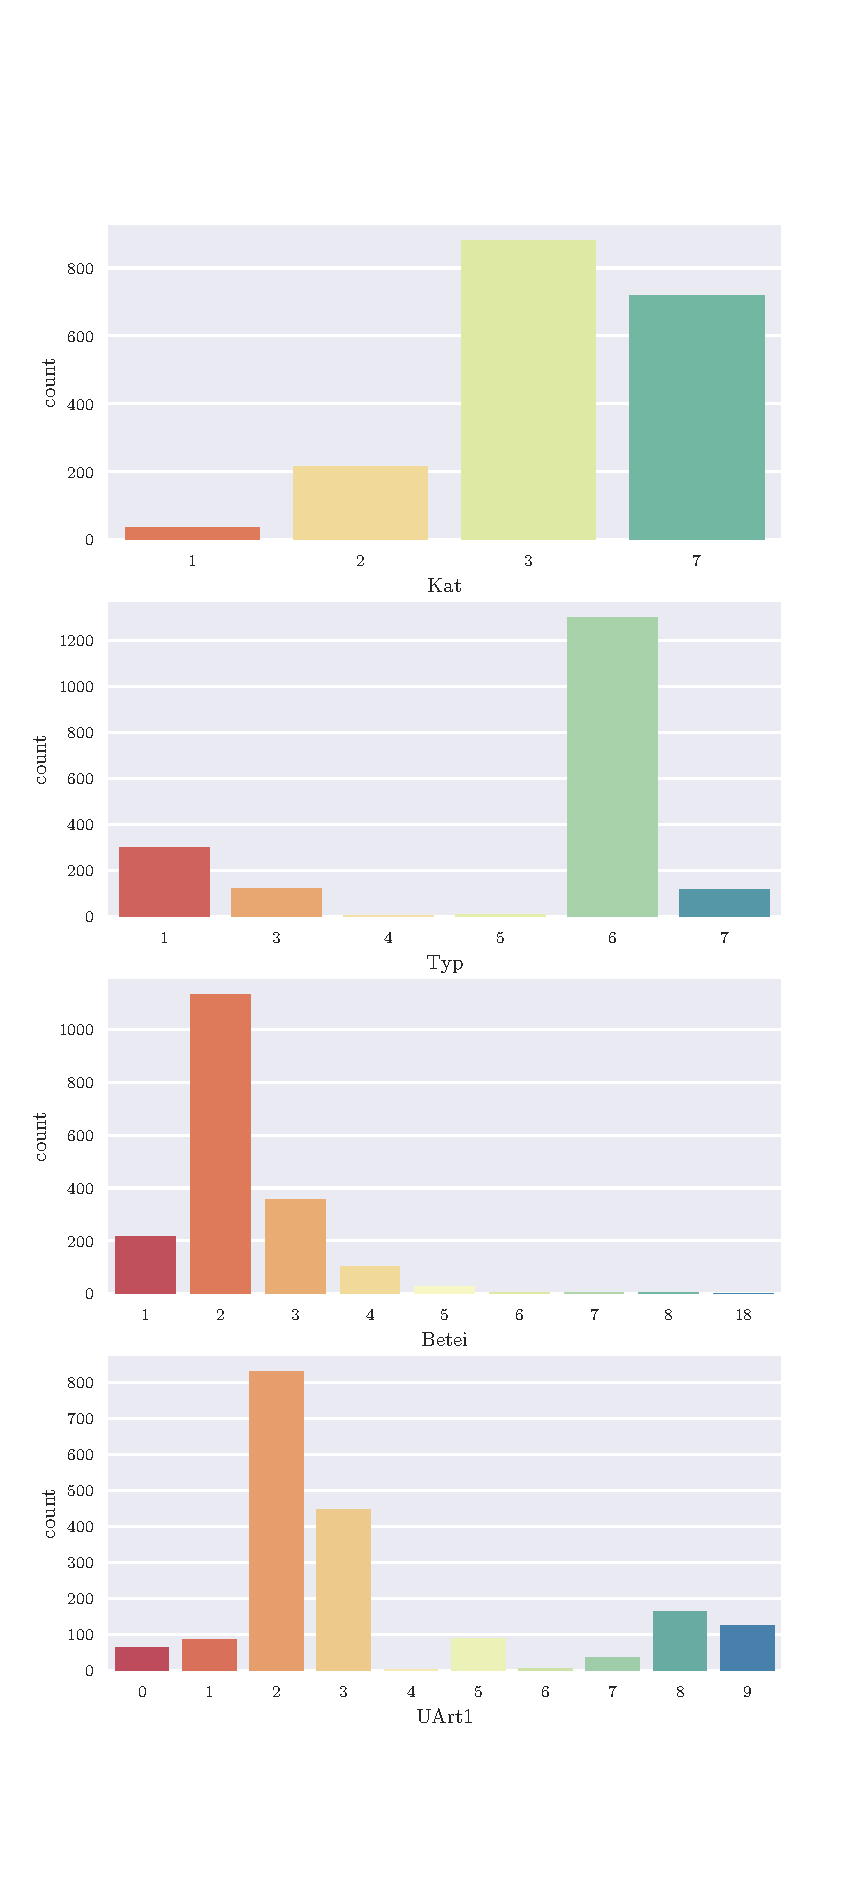
\includegraphics[scale=0.7]{CorrAnalysis/data/BAYSIS/02_matched/plots/baysis_matched_count_multiple01}
    %     \caption{Distribution of the accident category Kat, Typ, Betei and UArt}
    %     \label{img:baysis_matched_Kat}
    %     \label{img:baysis_matched_Typ}
    %     \label{img:baysis_matched_Betei}
    %     \label{img:baysis_matched_UArt}
    % \end{figure}

    % \begin{figure}[ht!]
    %     \centering
    %     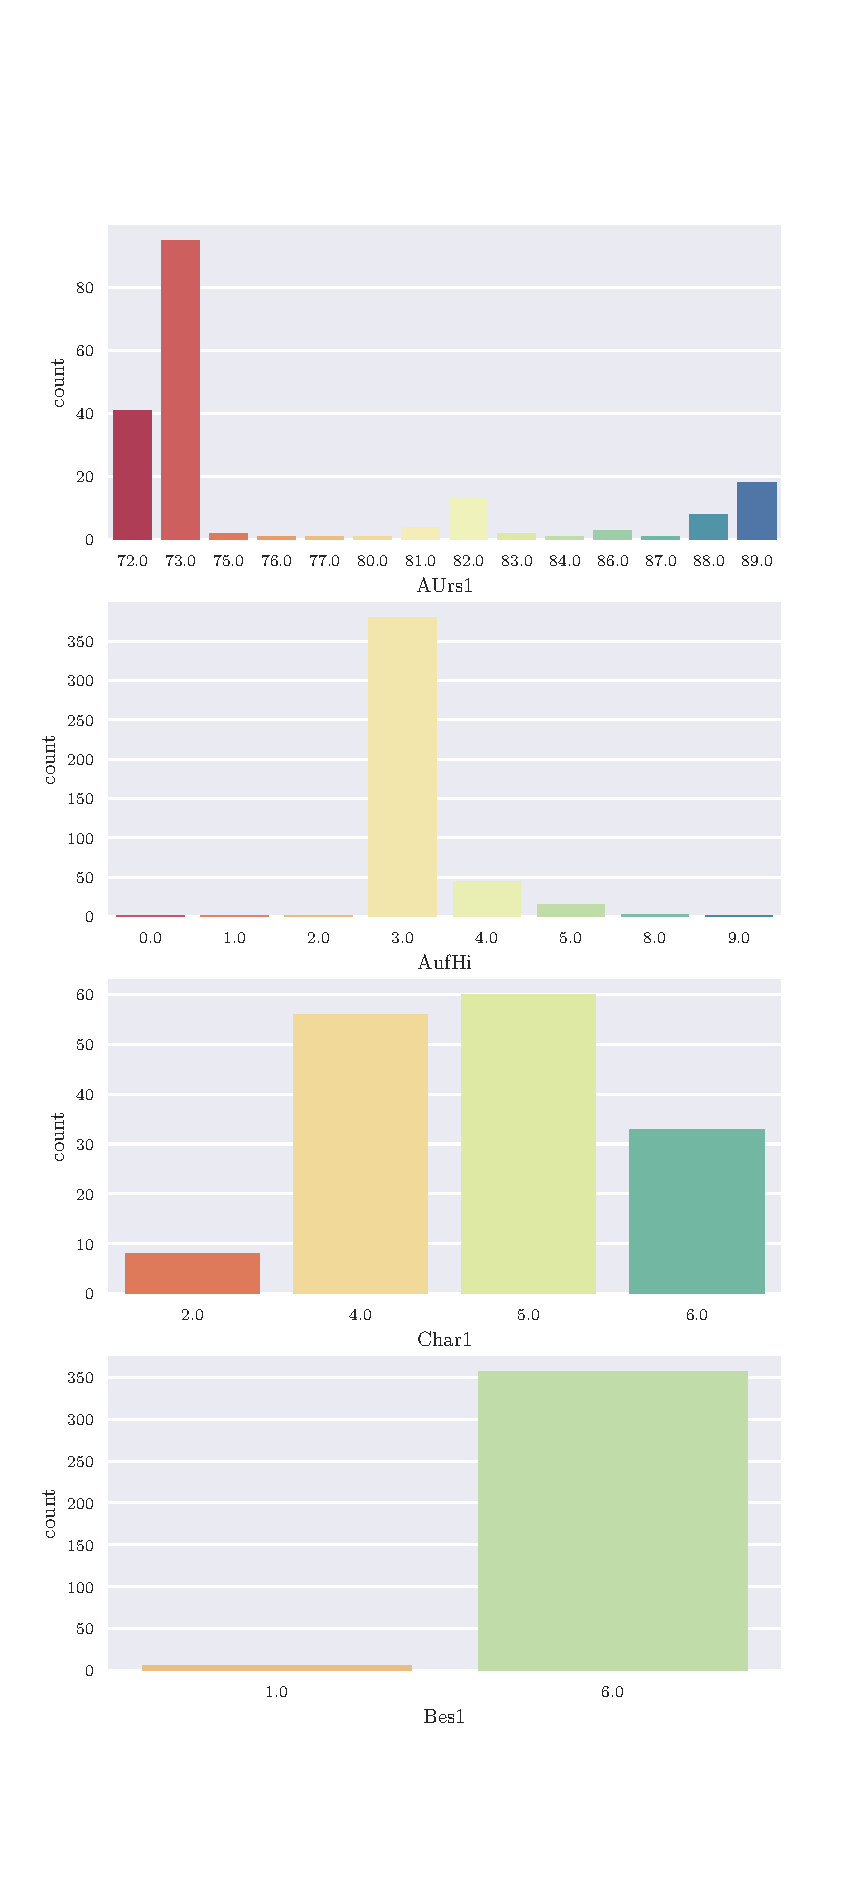
\includegraphics[scale=0.7]{CorrAnalysis/data/BAYSIS/02_matched/plots/baysis_matched_count_multiple02}
    %     \caption{Distribution of the accident category AUrs, AufHi, Char and Bes}
    %     \label{img:baysis_matched_AUrs}
    %     \label{img:baysis_matched_AufHi}
    %     \label{img:baysis_matched_Char}
    %     \label{img:baysis_matched_Bes}
    % \end{figure}

    % \begin{figure}[ht!]
    %     \centering
    %     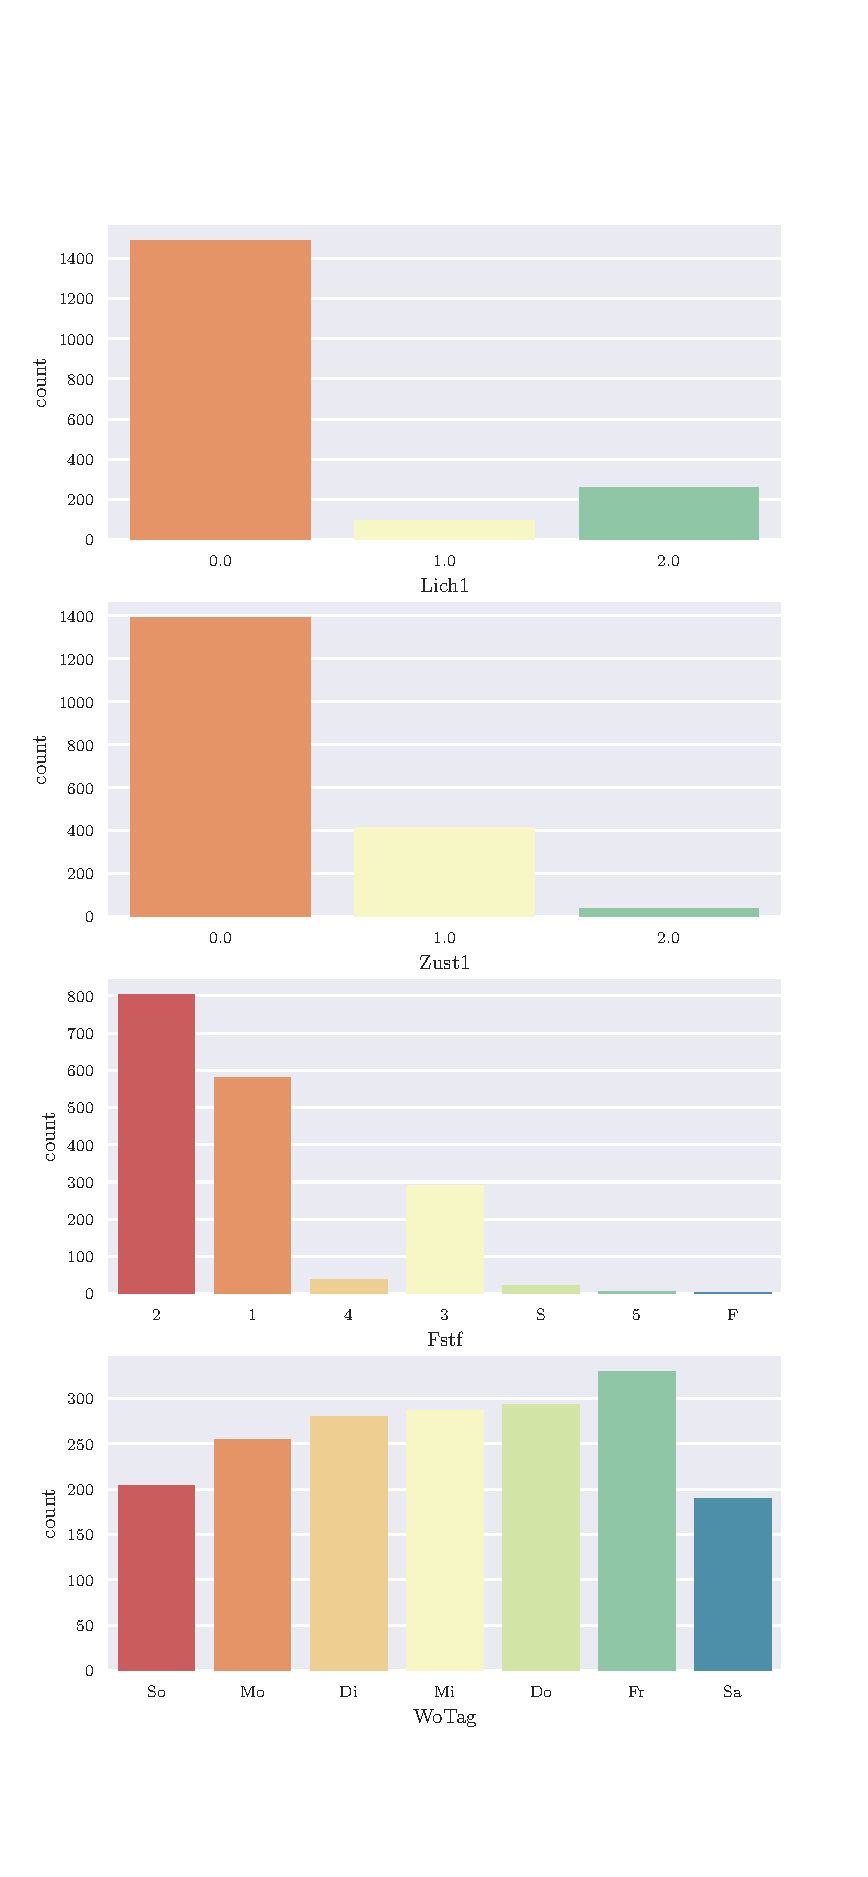
\includegraphics[scale=0.7]{CorrAnalysis/data/BAYSIS/02_matched/plots/baysis_matched_count_multiple03}
    %     \caption{Distribution of the accident category Lich, Zust, Fstf and WoTag}
    %     \label{img:baysis_matched_Lich}
    %     \label{img:baysis_matched_Zust}
    %     \label{img:baysis_matched_Fstf}
    %     \label{img:baysis_matched_WoTag}
    % \end{figure}
    
    % ------- BAYSIS Selected02 - Tables --------
    % \newgeometry{left=1cm,right=1cm,top=1cm}
    \begin{sidewaystable}
    	\tiny
    	\setlength{\tabcolsep}{2pt}
    	\centering
    	\begin{tabular}{lrrrrrrrrrrrrrrrrrrrrrrrrrrrrr}
\toprule
{} &  TMax &  TAvg &  SMax &  SAvg &  TDist &  SDist &   Cov &  TLCar &  TLHGV &  Str &  Kat &  Typ &  Betei &  UArt1 &  UArt2 &  AUrs1 &  AUrs2 &  AufHi &  Alkoh &  Char1 &  Char2 &  Lich1 &  Lich2 &  Zust1 &  Zust2 &  Fstf &  WoTag &  FeiTag &  Month \\
\midrule
TMax   &  1.00 &  0.80 &  0.50 &  0.43 &   0.00 &   0.00 & -0.19 &   0.03 &  -0.03 & 0.28 & 0.15 & 0.05 &   0.07 &   0.06 &   0.09 &   0.12 &   0.02 &   0.16 &  -0.02 &   0.09 &   0.05 &   0.05 &   0.05 &   0.11 &   0.03 &  0.00 &   0.12 &    0.03 &   0.19 \\
TAvg   &  0.80 &  1.00 &  0.22 &  0.46 &   0.00 &   0.00 &  0.18 &   0.03 &  -0.02 & 0.24 & 0.16 & 0.08 &   0.09 &   0.08 &   0.08 &   0.09 &   0.01 &   0.24 &   0.02 &   0.03 &   0.04 &   0.05 &   0.02 &   0.08 &   0.00 &  0.02 &   0.15 &    0.02 &   0.18 \\
SMax   &  0.50 &  0.22 &  1.00 &  0.62 &   0.00 &   0.00 & -0.48 &   0.00 &  -0.09 & 0.36 & 0.16 & 0.05 &   0.05 &   0.12 &   0.08 &   0.08 &   0.02 &   0.09 &  -0.05 &   0.10 &   0.02 &   0.06 &   0.05 &   0.08 &   0.05 &  0.06 &   0.11 &    0.07 &   0.19 \\
SAvg   &  0.43 &  0.46 &  0.62 &  1.00 &   0.00 &   0.00 &  0.18 &  -0.03 &  -0.10 & 0.31 & 0.24 & 0.04 &   0.10 &   0.17 &   0.10 &   0.13 &   0.03 &   0.04 &  -0.03 &   0.06 &   0.00 &   0.01 &   0.02 &   0.08 &   0.11 &  0.10 &   0.11 &    0.07 &   0.17 \\
TDist  &  0.00 &  0.00 &  0.00 &  0.00 &   0.00 &   0.00 &  0.00 &   0.00 &   0.00 & 0.00 & 0.00 & 0.00 &   0.00 &   0.00 &   0.00 &   0.00 &   0.00 &   0.00 &   0.00 &   0.00 &   0.00 &   0.00 &   0.00 &   0.00 &   0.00 &  0.00 &   0.00 &    0.00 &   0.00 \\
SDist  &  0.00 &  0.00 &  0.00 &  0.00 &   0.00 &   0.00 &  0.00 &   0.00 &   0.00 & 0.00 & 0.00 & 0.00 &   0.00 &   0.00 &   0.00 &   0.00 &   0.00 &   0.00 &   0.00 &   0.00 &   0.00 &   0.00 &   0.00 &   0.00 &   0.00 &  0.00 &   0.00 &    0.00 &   0.00 \\
Cov    & -0.19 &  0.18 & -0.48 &  0.18 &   0.00 &   0.00 &  1.00 &  -0.05 &   0.04 & 0.31 & 0.07 & 0.11 &   0.05 &   0.11 &   0.14 &   0.12 &   0.06 &   0.11 &   0.05 &   0.12 &   0.03 &   0.13 &   0.10 &   0.11 &   0.00 &  0.06 &   0.20 &   -0.01 &   0.19 \\
TLCar  &  0.03 &  0.03 &  0.00 & -0.03 &   0.00 &   0.00 & -0.05 &   1.00 &   0.00 & 0.12 & 0.01 & 0.11 &   0.00 &   0.11 &   0.10 &   0.12 &   0.03 &   0.05 &  -0.08 &   0.09 &   0.01 &   0.02 &   0.02 &   0.07 &   0.03 & -0.05 &   0.08 &   -0.04 &   0.10 \\
TLHGV  & -0.03 & -0.02 & -0.09 & -0.10 &   0.00 &   0.00 &  0.04 &   0.00 &   1.00 & 0.21 & 0.13 & 0.10 &   0.01 &   0.08 &   0.08 &   0.14 &   0.07 &   0.05 &  -0.05 &   0.12 &   0.01 &   0.03 &   0.03 &   0.11 &   0.05 & -0.01 &   0.14 &    0.05 &   0.21 \\
Str    &  0.28 &  0.24 &  0.36 &  0.31 &   0.00 &   0.00 &  0.31 &   0.12 &   0.21 & 1.00 & 0.14 & 0.15 &   0.12 &   0.20 &   0.15 &   0.14 &   0.11 &   0.12 &   0.08 &   0.22 &   0.15 &   0.18 &   0.16 &   0.22 &   0.14 &  0.18 &   0.16 &    0.12 &   0.15 \\
Kat    &  0.15 &  0.16 &  0.16 &  0.24 &   0.00 &   0.00 &  0.07 &   0.01 &   0.13 & 0.14 & 1.00 & 0.22 &   0.27 &   0.38 &   0.11 &   0.07 &   0.04 &   0.06 &   0.12 &   0.08 &   0.05 &   0.07 &   0.06 &   0.05 &   0.07 &  0.10 &   0.13 &    0.08 &   0.12 \\
Typ    &  0.05 &  0.08 &  0.05 &  0.04 &   0.00 &   0.00 &  0.11 &   0.11 &   0.10 & 0.15 & 0.22 & 1.00 &   0.32 &   0.51 &   0.10 &   0.27 &   0.08 &   0.25 &   0.07 &   0.14 &   0.13 &   0.12 &   0.13 &   0.16 &   0.26 &  0.14 &   0.13 &    0.08 &   0.15 \\
Betei  &  0.07 &  0.09 &  0.05 &  0.10 &   0.00 &   0.00 &  0.05 &   0.00 &   0.01 & 0.12 & 0.27 & 0.32 &   1.00 &   0.34 &   0.10 &   0.15 &   0.02 &   0.29 &   0.10 &   0.09 &   0.10 &   0.10 &   0.06 &   0.09 &   0.22 &  0.12 &   0.12 &    0.12 &   0.15 \\
UArt1  &  0.06 &  0.08 &  0.12 &  0.17 &   0.00 &   0.00 &  0.11 &   0.11 &   0.08 & 0.20 & 0.38 & 0.51 &   0.34 &   1.00 &   0.17 &   0.24 &   0.11 &   0.39 &   0.09 &   0.16 &   0.15 &   0.08 &   0.07 &   0.15 &   0.22 &  0.16 &   0.13 &    0.09 &   0.13 \\
UArt2  &  0.09 &  0.08 &  0.08 &  0.10 &   0.00 &   0.00 &  0.14 &   0.10 &   0.08 & 0.15 & 0.11 & 0.10 &   0.10 &   0.17 &   1.00 &   0.10 &   0.01 &   0.39 &   0.03 &   0.09 &   0.12 &   0.09 &   0.07 &   0.10 &   0.10 &  0.10 &   0.10 &    0.03 &   0.11 \\
AUrs1  &  0.12 &  0.09 &  0.08 &  0.13 &   0.00 &   0.00 &  0.12 &   0.12 &   0.14 & 0.14 & 0.07 & 0.27 &   0.15 &   0.24 &   0.10 &   1.00 &   0.28 &   0.30 &   0.03 &   0.07 &   0.02 &   0.10 &   0.08 &   0.42 &   0.52 &  0.05 &   0.10 &    0.06 &   0.18 \\
AUrs2  &  0.02 &  0.01 &  0.02 &  0.03 &   0.00 &   0.00 &  0.06 &   0.03 &   0.07 & 0.11 & 0.04 & 0.08 &   0.02 &   0.11 &   0.01 &   0.28 &   1.00 &   0.01 &   0.01 &   0.01 &   0.01 &   0.12 &   0.06 &   0.29 &   0.01 &  0.05 &   0.10 &    0.01 &   0.15 \\
AufHi  &  0.16 &  0.24 &  0.09 &  0.04 &   0.00 &   0.00 &  0.11 &   0.05 &   0.05 & 0.12 & 0.06 & 0.25 &   0.29 &   0.39 &   0.39 &   0.30 &   0.01 &   1.00 &   0.02 &   0.05 &   0.15 &   0.05 &   0.06 &   0.12 &   0.15 &  0.11 &   0.11 &    0.02 &   0.13 \\
Alkoh  & -0.02 &  0.02 & -0.05 & -0.03 &   0.00 &   0.00 &  0.05 &  -0.08 &  -0.05 & 0.08 & 0.12 & 0.07 &   0.10 &   0.09 &   0.03 &   0.03 &   0.01 &   0.02 &   1.00 &   0.09 &   0.05 &   0.14 &   0.14 &   0.08 &   0.05 &  0.04 &   0.08 &    0.02 &   0.09 \\
Char1  &  0.09 &  0.03 &  0.10 &  0.06 &   0.00 &   0.00 &  0.12 &   0.09 &   0.12 & 0.22 & 0.08 & 0.14 &   0.09 &   0.16 &   0.09 &   0.07 &   0.01 &   0.05 &   0.09 &   1.00 &   0.48 &   0.07 &   0.04 &   0.05 &   0.08 &  0.10 &   0.10 &    0.04 &   0.12 \\
Char2  &  0.05 &  0.04 &  0.02 &  0.00 &   0.00 &   0.00 &  0.03 &   0.01 &   0.01 & 0.15 & 0.05 & 0.13 &   0.10 &   0.15 &   0.12 &   0.02 &   0.01 &   0.15 &   0.05 &   0.48 &   1.00 &   0.06 &   0.04 &   0.03 &   0.06 &  0.08 &   0.10 &    0.04 &   0.12 \\
Lich1  &  0.05 &  0.05 &  0.06 &  0.01 &   0.00 &   0.00 &  0.13 &   0.02 &   0.03 & 0.18 & 0.07 & 0.12 &   0.10 &   0.08 &   0.09 &   0.10 &   0.12 &   0.05 &   0.14 &   0.07 &   0.06 &   1.00 &   0.71 &   0.13 &   0.05 &  0.09 &   0.12 &    0.03 &   0.32 \\
Lich2  &  0.05 &  0.02 &  0.05 &  0.02 &   0.00 &   0.00 &  0.10 &   0.02 &   0.03 & 0.16 & 0.06 & 0.13 &   0.06 &   0.07 &   0.07 &   0.08 &   0.06 &   0.06 &   0.14 &   0.04 &   0.04 &   0.71 &   1.00 &   0.13 &   0.04 &  0.09 &   0.11 &    0.01 &   0.32 \\
Zust1  &  0.11 &  0.08 &  0.08 &  0.08 &   0.00 &   0.00 &  0.11 &   0.07 &   0.11 & 0.22 & 0.05 & 0.16 &   0.09 &   0.15 &   0.10 &   0.42 &   0.29 &   0.12 &   0.08 &   0.05 &   0.03 &   0.13 &   0.13 &   1.00 &   0.22 &  0.07 &   0.11 &    0.05 &   0.27 \\
Zust2  &  0.03 &  0.00 &  0.05 &  0.11 &   0.00 &   0.00 &  0.00 &   0.03 &   0.05 & 0.14 & 0.07 & 0.26 &   0.22 &   0.22 &   0.10 &   0.52 &   0.01 &   0.15 &   0.05 &   0.08 &   0.06 &   0.05 &   0.04 &   0.22 &   1.00 &  0.08 &   0.10 &    0.04 &   0.25 \\
Fstf   &  0.00 &  0.02 &  0.06 &  0.10 &   0.00 &   0.00 &  0.06 &  -0.05 &  -0.01 & 0.18 & 0.10 & 0.14 &   0.12 &   0.16 &   0.10 &   0.05 &   0.05 &   0.11 &   0.04 &   0.10 &   0.08 &   0.09 &   0.09 &   0.07 &   0.08 &  1.00 &   0.10 &    0.13 &   0.13 \\
WoTag  &  0.12 &  0.15 &  0.11 &  0.11 &   0.00 &   0.00 &  0.20 &   0.08 &   0.14 & 0.16 & 0.13 & 0.13 &   0.12 &   0.13 &   0.10 &   0.10 &   0.10 &   0.11 &   0.08 &   0.10 &   0.10 &   0.12 &   0.11 &   0.11 &   0.10 &  0.10 &   1.00 &    0.14 &   0.16 \\
FeiTag &  0.03 &  0.02 &  0.07 &  0.07 &   0.00 &   0.00 & -0.01 &  -0.04 &   0.05 & 0.12 & 0.08 & 0.08 &   0.12 &   0.09 &   0.03 &   0.06 &   0.01 &   0.02 &   0.02 &   0.04 &   0.04 &   0.03 &   0.01 &   0.05 &   0.04 &  0.13 &   0.14 &    1.00 &   0.16 \\
Month  &  0.19 &  0.18 &  0.19 &  0.17 &   0.00 &   0.00 &  0.19 &   0.10 &   0.21 & 0.15 & 0.12 & 0.15 &   0.15 &   0.13 &   0.11 &   0.18 &   0.15 &   0.13 &   0.09 &   0.12 &   0.12 &   0.32 &   0.32 &   0.27 &   0.25 &  0.13 &   0.16 &    0.16 &   1.00 \\
\bottomrule
\end{tabular}

    	\caption{Correlation matrix for BAYSIS selected data (Jam Effector), calculated with Cramer's $V$, $\eta$, $\tau$, $r_{pq}$, $r$}
    	\label{table:appendix_correlation_matrix_selected_duringJam_cramers}
    \end{sidewaystable}  
    \begin{sidewaystable}
    	\tiny
    	\setlength{\tabcolsep}{2pt}
    	\centering
    	\begin{tabular}{lrrrrrrrrrrrrrrrrrrrrrrrrrrrrr}
\toprule
{} &  TMax &  TAvg &  SMax &  SAvg &  TDist &  SDist &   Cov &  TLCar &  TLHGV &  Str &  Kat &  Typ &  Betei &  UArt1 &  UArt2 &  AUrs1 &  AUrs2 &  AufHi &  Alkoh &  Char1 &  Char2 &  Lich1 &  Lich2 &  Zust1 &  Zust2 &  Fstf &  WoTag &  FeiTag &  Month \\
\midrule
TMax   &  1.00 &  0.80 &  0.50 &  0.43 &   0.00 &   0.00 & -0.19 &   0.03 &  -0.03 & 0.28 & 0.15 & 0.05 &   0.07 &   0.06 &   0.09 &   0.12 &   0.02 &   0.16 &  -0.02 &   0.09 &   0.05 &   0.05 &   0.05 &   0.11 &   0.03 &  0.00 &   0.12 &    0.03 &   0.19 \\
TAvg   &  0.80 &  1.00 &  0.22 &  0.46 &   0.00 &   0.00 &  0.18 &   0.03 &  -0.02 & 0.24 & 0.16 & 0.08 &   0.09 &   0.08 &   0.08 &   0.09 &   0.01 &   0.24 &   0.02 &   0.03 &   0.04 &   0.05 &   0.02 &   0.08 &   0.00 &  0.02 &   0.15 &    0.02 &   0.18 \\
SMax   &  0.50 &  0.22 &  1.00 &  0.62 &   0.00 &   0.00 & -0.48 &   0.00 &  -0.09 & 0.36 & 0.16 & 0.05 &   0.05 &   0.12 &   0.08 &   0.08 &   0.02 &   0.09 &  -0.05 &   0.10 &   0.02 &   0.06 &   0.05 &   0.08 &   0.05 &  0.06 &   0.11 &    0.07 &   0.19 \\
SAvg   &  0.43 &  0.46 &  0.62 &  1.00 &   0.00 &   0.00 &  0.18 &  -0.03 &  -0.10 & 0.31 & 0.24 & 0.04 &   0.10 &   0.17 &   0.10 &   0.13 &   0.03 &   0.04 &  -0.03 &   0.06 &   0.00 &   0.01 &   0.02 &   0.08 &   0.11 &  0.10 &   0.11 &    0.07 &   0.17 \\
TDist  &  0.00 &  0.00 &  0.00 &  0.00 &   0.00 &   0.00 &  0.00 &   0.00 &   0.00 & 0.00 & 0.00 & 0.00 &   0.00 &   0.00 &   0.00 &   0.00 &   0.00 &   0.00 &   0.00 &   0.00 &   0.00 &   0.00 &   0.00 &   0.00 &   0.00 &  0.00 &   0.00 &    0.00 &   0.00 \\
SDist  &  0.00 &  0.00 &  0.00 &  0.00 &   0.00 &   0.00 &  0.00 &   0.00 &   0.00 & 0.00 & 0.00 & 0.00 &   0.00 &   0.00 &   0.00 &   0.00 &   0.00 &   0.00 &   0.00 &   0.00 &   0.00 &   0.00 &   0.00 &   0.00 &   0.00 &  0.00 &   0.00 &    0.00 &   0.00 \\
Cov    & -0.19 &  0.18 & -0.48 &  0.18 &   0.00 &   0.00 &  1.00 &  -0.05 &   0.04 & 0.31 & 0.07 & 0.11 &   0.05 &   0.11 &   0.14 &   0.12 &   0.06 &   0.11 &   0.05 &   0.12 &   0.03 &   0.13 &   0.10 &   0.11 &   0.00 &  0.06 &   0.20 &   -0.01 &   0.19 \\
TLCar  &  0.03 &  0.03 &  0.00 & -0.03 &   0.00 &   0.00 & -0.05 &   1.00 &   0.00 & 0.12 & 0.01 & 0.11 &   0.00 &   0.11 &   0.10 &   0.12 &   0.03 &   0.05 &  -0.08 &   0.09 &   0.01 &   0.02 &   0.02 &   0.07 &   0.03 & -0.05 &   0.08 &   -0.04 &   0.10 \\
TLHGV  & -0.03 & -0.02 & -0.09 & -0.10 &   0.00 &   0.00 &  0.04 &   0.00 &   1.00 & 0.21 & 0.13 & 0.10 &   0.01 &   0.08 &   0.08 &   0.14 &   0.07 &   0.05 &  -0.05 &   0.12 &   0.01 &   0.03 &   0.03 &   0.11 &   0.05 & -0.01 &   0.14 &    0.05 &   0.21 \\
Str    &  0.28 &  0.24 &  0.36 &  0.31 &   0.00 &   0.00 &  0.31 &   0.12 &   0.21 & 1.00 & 0.02 & 0.02 &   0.02 &   0.04 &   0.02 &   0.02 &   0.00 &   0.01 &   0.00 &   0.02 &   0.00 &   0.01 &   0.01 &   0.01 &   0.00 &  0.05 &   0.05 &    0.00 &   0.06 \\
Kat    &  0.15 &  0.16 &  0.16 &  0.24 &   0.00 &   0.00 &  0.07 &   0.01 &   0.13 & 0.03 & 1.00 & 0.09 &   0.13 &   0.27 &   0.02 &   0.01 &   0.00 &   0.01 &   0.00 &   0.01 &   0.00 &   0.01 &   0.01 &   0.01 &   0.00 &  0.02 &   0.03 &    0.00 &   0.02 \\
Typ    &  0.05 &  0.08 &  0.05 &  0.04 &   0.00 &   0.00 &  0.11 &   0.11 &   0.10 & 0.05 & 0.11 & 1.00 &   0.18 &   0.39 &   0.03 &   0.08 &   0.00 &   0.10 &   0.00 &   0.03 &   0.01 &   0.01 &   0.01 &   0.04 &   0.02 &  0.05 &   0.04 &    0.00 &   0.05 \\
Betei  &  0.07 &  0.09 &  0.05 &  0.10 &   0.00 &   0.00 &  0.05 &   0.00 &   0.01 & 0.04 & 0.14 & 0.16 &   1.00 &   0.25 &   0.02 &   0.04 &   0.00 &   0.09 &   0.01 &   0.01 &   0.00 &   0.01 &   0.01 &   0.01 &   0.01 &  0.04 &   0.04 &    0.01 &   0.06 \\
UArt1  &  0.06 &  0.08 &  0.12 &  0.17 &   0.00 &   0.00 &  0.11 &   0.11 &   0.08 & 0.05 & 0.17 & 0.22 &   0.15 &   1.00 &   0.03 &   0.05 &   0.00 &   0.12 &   0.00 &   0.02 &   0.01 &   0.01 &   0.00 &   0.02 &   0.01 &  0.05 &   0.04 &    0.00 &   0.04 \\
UArt2  &  0.09 &  0.08 &  0.08 &  0.10 &   0.00 &   0.00 &  0.14 &   0.10 &   0.08 & 0.10 & 0.05 & 0.05 &   0.05 &   0.13 &   1.00 &   0.04 &   0.00 &   0.45 &   0.00 &   0.03 &   0.01 &   0.02 &   0.01 &   0.03 &   0.01 &  0.06 &   0.07 &    0.00 &   0.09 \\
AUrs1  &  0.12 &  0.09 &  0.08 &  0.13 &   0.00 &   0.00 &  0.12 &   0.12 &   0.14 & 0.11 & 0.03 & 0.24 &   0.12 &   0.24 &   0.05 &   1.00 &   0.04 &   0.17 &   0.00 &   0.02 &   0.00 &   0.03 &   0.02 &   0.31 &   0.08 &  0.04 &   0.12 &    0.01 &   0.25 \\
AUrs2  &  0.02 &  0.01 &  0.02 &  0.03 &   0.00 &   0.00 &  0.06 &   0.03 &   0.07 & 0.26 & 0.11 & 0.18 &   0.04 &   0.24 &   0.01 &   0.54 &   1.00 &   0.02 &   0.00 &   0.01 &   0.00 &   0.21 &   0.14 &   0.55 &   0.00 &  0.13 &   0.28 &    0.00 &   0.37 \\
AufHi  &  0.16 &  0.24 &  0.09 &  0.04 &   0.00 &   0.00 &  0.11 &   0.05 &   0.05 & 0.06 & 0.01 & 0.20 &   0.20 &   0.42 &   0.43 &   0.12 &   0.00 &   1.00 &   0.00 &   0.01 &   0.01 &   0.00 &   0.01 &   0.04 &   0.01 &  0.05 &   0.05 &    0.00 &   0.07 \\
Alkoh  & -0.02 &  0.02 & -0.05 & -0.03 &   0.00 &   0.00 &  0.05 &  -0.08 &  -0.05 & 0.04 & 0.05 & 0.05 &   0.06 &   0.08 &   0.01 &   0.01 &   0.00 &   0.00 &   1.00 &   0.03 &   0.03 &   0.08 &   0.09 &   0.02 &   0.00 &  0.01 &   0.05 &    0.00 &   0.08 \\
Char1  &  0.09 &  0.03 &  0.10 &  0.06 &   0.00 &   0.00 &  0.12 &   0.09 &   0.12 & 0.14 & 0.03 & 0.08 &   0.04 &   0.09 &   0.03 &   0.02 &   0.00 &   0.02 &   0.01 &   1.00 &   0.10 &   0.01 &   0.01 &   0.01 &   0.01 &  0.06 &   0.06 &    0.00 &   0.10 \\
Char2  &  0.05 &  0.04 &  0.02 &  0.00 &   0.00 &   0.00 &  0.03 &   0.01 &   0.01 & 0.12 & 0.03 & 0.11 &   0.06 &   0.16 &   0.06 &   0.01 &   0.00 &   0.12 &   0.04 &   0.58 &   1.00 &   0.03 &   0.01 &   0.01 &   0.00 &  0.07 &   0.11 &    0.00 &   0.15 \\
Lich1  &  0.05 &  0.05 &  0.06 &  0.01 &   0.00 &   0.00 &  0.13 &   0.02 &   0.03 & 0.05 & 0.01 & 0.02 &   0.02 &   0.02 &   0.02 &   0.02 &   0.01 &   0.00 &   0.01 &   0.01 &   0.00 &   1.00 &   0.82 &   0.03 &   0.00 &  0.01 &   0.03 &    0.00 &   0.19 \\
Lich2  &  0.05 &  0.02 &  0.05 &  0.02 &   0.00 &   0.00 &  0.10 &   0.02 &   0.03 & 0.05 & 0.01 & 0.02 &   0.01 &   0.01 &   0.01 &   0.01 &   0.01 &   0.01 &   0.01 &   0.00 &   0.00 &   0.92 &   1.00 &   0.03 &   0.00 &  0.01 &   0.02 &    0.00 &   0.21 \\
Zust1  &  0.11 &  0.08 &  0.08 &  0.08 &   0.00 &   0.00 &  0.11 &   0.07 &   0.11 & 0.05 & 0.01 & 0.06 &   0.02 &   0.05 &   0.02 &   0.17 &   0.02 &   0.03 &   0.00 &   0.01 &   0.00 &   0.03 &   0.03 &   1.00 &   0.03 &  0.02 &   0.03 &    0.00 &   0.17 \\
Zust2  &  0.03 &  0.00 &  0.05 &  0.11 &   0.00 &   0.00 &  0.00 &   0.03 &   0.05 & 0.16 & 0.06 & 0.31 &   0.19 &   0.20 &   0.06 &   0.43 &   0.00 &   0.12 &   0.00 &   0.03 &   0.00 &   0.01 &   0.01 &   0.32 &   1.00 &  0.06 &   0.11 &    0.00 &   0.34 \\
Fstf   &  0.00 &  0.02 &  0.06 &  0.10 &   0.00 &   0.00 &  0.06 &  -0.05 &  -0.01 & 0.08 & 0.01 & 0.03 &   0.03 &   0.06 &   0.02 &   0.01 &   0.00 &   0.02 &   0.00 &   0.01 &   0.00 &   0.00 &   0.00 &   0.01 &   0.00 &  1.00 &   0.03 &    0.00 &   0.04 \\
WoTag  &  0.12 &  0.15 &  0.11 &  0.11 &   0.00 &   0.00 &  0.20 &   0.08 &   0.14 & 0.05 & 0.01 & 0.02 &   0.02 &   0.03 &   0.01 &   0.02 &   0.00 &   0.01 &   0.00 &   0.01 &   0.00 &   0.01 &   0.01 &   0.01 &   0.00 &  0.02 &   1.00 &    0.01 &   0.04 \\
FeiTag &  0.03 &  0.02 &  0.07 &  0.07 &   0.00 &   0.00 & -0.01 &  -0.04 &   0.05 & 0.09 & 0.04 & 0.04 &   0.07 &   0.07 &   0.01 &   0.02 &   0.00 &   0.00 &   0.00 &   0.01 &   0.00 &   0.01 &   0.00 &   0.01 &   0.00 &  0.03 &   0.11 &    1.00 &   0.15 \\
Month  &  0.19 &  0.18 &  0.19 &  0.17 &   0.00 &   0.00 &  0.19 &   0.10 &   0.21 & 0.05 & 0.01 & 0.02 &   0.02 &   0.03 &   0.01 &   0.03 &   0.00 &   0.01 &   0.00 &   0.01 &   0.00 &   0.04 &   0.04 &   0.04 &   0.01 &  0.02 &   0.03 &    0.01 &   1.00 \\
\bottomrule
\end{tabular}

    	\caption{Correlation matrix for BAYSIS selected data (Jam Effector), calculated with Theil's $U$, $\eta$, $\tau$, $r_{pq}$, $r$}
    	\label{table:appendix_correlation_matrix_selected_duringJam_theils}
    \end{sidewaystable}
    \begin{sidewaystable}
    	\tiny
    	\setlength{\tabcolsep}{2pt}
    	\centering
    	\begin{tabular}{lrrrrrrrrrrrrrrrrrrrrrrrrrrrrr}
\toprule
{} &  TMax &  TAvg &  SMax &  SAvg &  TDist &  SDist &   Cov &  TLCar &  TLHGV &   Str &   Kat &   Typ &  Betei &  UArt1 &  UArt2 &  AUrs1 &  AUrs2 &  AufHi &  Alkoh &  Char1 &  Char2 &  Lich1 &  Lich2 &  Zust1 &  Zust2 &  Fstf &  WoTag &  FeiTag &  Month \\
\midrule
TMax   &   nan & 0.000 & 0.000 & 0.000 &    nan &    nan & 0.000 &  0.363 &  0.495 & 0.000 & 0.000 & 0.000 &  0.011 &  0.000 &  0.000 &  0.000 &  0.000 &  0.000 &  0.577 &  0.000 &  0.000 &  0.000 &  0.000 &  0.000 &  0.000 & 0.979 &  0.000 &   0.345 &  0.000 \\
TAvg   & 0.000 &   nan & 0.000 & 0.000 &    nan &    nan & 0.000 &  0.494 &  0.560 & 0.000 & 0.000 & 0.000 &  0.003 &  0.000 &  0.000 &  0.000 &  0.000 &  0.000 &  0.595 &  0.000 &  0.000 &  0.000 &  0.000 &  0.000 &  0.000 & 0.489 &  0.000 &   0.577 &  0.000 \\
SMax   & 0.000 & 0.000 &   nan & 0.000 &    nan &    nan & 0.000 &  0.960 &  0.014 & 0.000 & 0.000 & 0.000 &  0.077 &  0.000 &  0.000 &  0.000 &  0.000 &  0.000 &  0.170 &  0.000 &  0.000 &  0.000 &  0.000 &  0.000 &  0.000 & 0.021 &  0.000 &   0.030 &  0.000 \\
SAvg   & 0.000 & 0.000 & 0.000 &   nan &    nan &    nan & 0.000 &  0.436 &  0.005 & 0.000 & 0.000 & 0.000 &  0.000 &  0.000 &  0.000 &  0.000 &  0.000 &  0.000 &  0.423 &  0.000 &  0.000 &  0.000 &  0.000 &  0.000 &  0.000 & 0.001 &  0.000 &   0.023 &  0.000 \\
TDist  &   nan &   nan &   nan &   nan &    nan &    nan &   nan &    nan &    nan &   nan &   nan &   nan &    nan &    nan &    nan &    nan &    nan &    nan &    nan &    nan &    nan &    nan &    nan &    nan &    nan &   nan &    nan &     nan &    nan \\
SDist  &   nan &   nan &   nan &   nan &    nan &    nan &   nan &    nan &    nan &   nan &   nan &   nan &    nan &    nan &    nan &    nan &    nan &    nan &    nan &    nan &    nan &    nan &    nan &    nan &    nan &   nan &    nan &     nan &    nan \\
Cov    & 0.000 & 0.000 & 0.000 & 0.000 &    nan &    nan &   nan &  0.194 &  0.263 & 0.000 & 0.000 & 0.000 &  0.062 &  0.000 &  0.000 &  0.000 &  0.000 &  0.000 &  0.135 &  0.000 &  0.000 &  0.000 &  0.000 &  0.000 &  0.000 & 0.038 &  0.000 &   0.777 &  0.000 \\
TLCar  & 0.363 & 0.494 & 0.960 & 0.436 &    nan &    nan & 0.194 &    nan &  1.000 & 0.000 & 0.000 & 0.000 &  0.875 &  0.000 &  0.000 &  0.000 &  0.000 &  0.000 &  0.028 &  0.000 &  0.000 &  0.000 &  0.000 &  0.000 &  0.000 & 0.078 &  0.000 &   0.242 &  0.000 \\
TLHGV  & 0.495 & 0.560 & 0.014 & 0.005 &    nan &    nan & 0.263 &  1.000 &    nan & 0.000 & 0.000 & 0.000 &  0.690 &  0.000 &  0.000 &  0.000 &  0.000 &  0.000 &  0.201 &  0.000 &  0.000 &  0.000 &  0.000 &  0.000 &  0.000 & 0.700 &  0.000 &   0.119 &  0.000 \\
Str    & 0.000 & 0.000 & 0.000 & 0.000 &    nan &    nan & 0.000 &  0.000 &  0.000 &   nan & 0.265 & 0.102 &  0.790 &  0.000 &  0.067 &  0.163 &  0.840 &  0.838 &  0.989 &  0.000 &  0.203 &  0.005 &  0.041 &  0.000 &  0.378 & 0.000 &  0.001 &   0.660 &  0.024 \\
Kat    & 0.000 & 0.000 & 0.000 & 0.000 &    nan &    nan & 0.000 &  0.000 &  0.000 & 0.265 &   nan & 0.000 &  0.000 &  0.000 &  0.064 &  0.934 &  0.847 &  0.808 &  0.012 &  0.232 &  0.670 &  0.321 &  0.467 &  0.828 &  0.291 & 0.306 &  0.013 &   0.161 &  0.537 \\
Typ    & 0.000 & 0.000 & 0.000 & 0.000 &    nan &    nan & 0.000 &  0.000 &  0.000 & 0.102 & 0.000 &   nan &  0.000 &  0.000 &  0.196 &  0.000 &  0.227 &  0.000 &  0.478 &  0.000 &  0.012 &  0.008 &  0.003 &  0.000 &  0.000 & 0.001 &  0.008 &   0.323 &  0.031 \\
Betei  & 0.011 & 0.003 & 0.077 & 0.000 &    nan &    nan & 0.062 &  0.875 &  0.690 & 0.790 & 0.000 & 0.000 &    nan &  0.000 &  0.178 &  0.000 &  1.000 &  0.000 &  0.268 &  0.531 &  0.303 &  0.339 &  0.915 &  0.477 &  0.000 & 0.024 &  0.033 &   0.081 &  0.005 \\
UArt1  & 0.000 & 0.000 & 0.000 & 0.000 &    nan &    nan & 0.000 &  0.000 &  0.000 & 0.000 & 0.000 & 0.000 &  0.000 &    nan &  0.000 &  0.000 &  0.361 &  0.000 &  0.589 &  0.000 &  0.031 &  0.832 &  0.956 &  0.002 &  0.000 & 0.000 &  0.003 &   0.576 &  0.276 \\
UArt2  & 0.000 & 0.000 & 0.000 & 0.000 &    nan &    nan & 0.000 &  0.000 &  0.000 & 0.067 & 0.064 & 0.196 &  0.178 &  0.000 &    nan &  0.223 &  1.000 &  0.000 &  0.994 &  0.433 &  0.109 &  0.442 &  0.879 &  0.164 &  0.228 & 0.541 &  0.234 &   0.996 &  0.900 \\
AUrs1  & 0.000 & 0.000 & 0.000 & 0.000 &    nan &    nan & 0.000 &  0.000 &  0.000 & 0.163 & 0.934 & 0.000 &  0.000 &  0.000 &  0.223 &    nan &  0.000 &  0.000 &  0.999 &  0.964 &  1.000 &  0.374 &  0.830 &  0.000 &  0.000 & 1.000 &  0.210 &   0.895 &  0.000 \\
AUrs2  & 0.000 & 0.000 & 0.000 & 0.000 &    nan &    nan & 0.000 &  0.000 &  0.000 & 0.840 & 0.847 & 0.227 &  1.000 &  0.361 &  1.000 &  0.000 &    nan &  1.000 &  0.985 &  1.000 &  0.991 &  0.000 &  0.199 &  0.000 &  0.991 & 0.997 &  0.398 &   0.981 &  0.075 \\
AufHi  & 0.000 & 0.000 & 0.000 & 0.000 &    nan &    nan & 0.000 &  0.000 &  0.000 & 0.838 & 0.808 & 0.000 &  0.000 &  0.000 &  0.000 &  0.000 &  1.000 &    nan &  0.995 &  0.930 &  0.003 &  0.934 &  0.782 &  0.002 &  0.003 & 0.219 &  0.077 &   0.980 &  0.148 \\
Alkoh  & 0.577 & 0.595 & 0.170 & 0.423 &    nan &    nan & 0.135 &  0.028 &  0.201 & 0.989 & 0.012 & 0.478 &  0.268 &  0.589 &  0.994 &  0.999 &  0.985 &  0.995 &    nan &  0.240 &  0.213 &  0.001 &  0.001 &  0.236 &  0.213 & 0.989 &  0.738 &   0.514 &  0.835 \\
Char1  & 0.000 & 0.000 & 0.000 & 0.000 &    nan &    nan & 0.000 &  0.000 &  0.000 & 0.000 & 0.232 & 0.000 &  0.531 &  0.000 &  0.433 &  0.964 &  1.000 &  0.930 &  0.240 &    nan &  0.000 &  0.488 &  0.946 &  0.921 &  0.353 & 0.476 &  0.259 &   0.918 &  0.502 \\
Char2  & 0.000 & 0.000 & 0.000 & 0.000 &    nan &    nan & 0.000 &  0.000 &  0.000 & 0.203 & 0.670 & 0.012 &  0.303 &  0.031 &  0.109 &  1.000 &  0.991 &  0.003 &  0.213 &  0.000 &    nan &  0.306 &  0.565 &  0.843 &  0.088 & 0.648 &  0.423 &   0.304 &  0.482 \\
Lich1  & 0.000 & 0.000 & 0.000 & 0.000 &    nan &    nan & 0.000 &  0.000 &  0.000 & 0.005 & 0.321 & 0.008 &  0.339 &  0.832 &  0.442 &  0.374 &  0.000 &  0.934 &  0.001 &  0.488 &  0.306 &    nan &  0.000 &  0.000 &  0.438 & 0.544 &  0.065 &   0.677 &  0.000 \\
Lich2  & 0.000 & 0.000 & 0.000 & 0.000 &    nan &    nan & 0.000 &  0.000 &  0.000 & 0.041 & 0.467 & 0.003 &  0.915 &  0.956 &  0.879 &  0.830 &  0.199 &  0.782 &  0.001 &  0.946 &  0.565 &  0.000 &    nan &  0.000 &  0.565 & 0.669 &  0.175 &   0.923 &  0.000 \\
Zust1  & 0.000 & 0.000 & 0.000 & 0.000 &    nan &    nan & 0.000 &  0.000 &  0.000 & 0.000 & 0.828 & 0.000 &  0.477 &  0.002 &  0.164 &  0.000 &  0.000 &  0.002 &  0.236 &  0.921 &  0.843 &  0.000 &  0.000 &    nan &  0.000 & 0.956 &  0.139 &   0.643 &  0.000 \\
Zust2  & 0.000 & 0.000 & 0.000 & 0.000 &    nan &    nan & 0.000 &  0.000 &  0.000 & 0.378 & 0.291 & 0.000 &  0.000 &  0.000 &  0.228 &  0.000 &  0.991 &  0.003 &  0.213 &  0.353 &  0.088 &  0.438 &  0.565 &  0.000 &    nan & 0.752 &  0.410 &   0.304 &  0.000 \\
Fstf   & 0.979 & 0.489 & 0.021 & 0.001 &    nan &    nan & 0.038 &  0.078 &  0.700 & 0.000 & 0.306 & 0.001 &  0.024 &  0.000 &  0.541 &  1.000 &  0.997 &  0.219 &  0.989 &  0.476 &  0.648 &  0.544 &  0.669 &  0.956 &  0.752 &   nan &  0.241 &   0.098 &  0.277 \\
WoTag  & 0.000 & 0.000 & 0.000 & 0.000 &    nan &    nan & 0.000 &  0.000 &  0.000 & 0.001 & 0.013 & 0.008 &  0.033 &  0.003 &  0.234 &  0.210 &  0.398 &  0.077 &  0.738 &  0.259 &  0.423 &  0.065 &  0.175 &  0.139 &  0.410 & 0.241 &    nan &   0.044 &  0.000 \\
FeiTag & 0.345 & 0.577 & 0.030 & 0.023 &    nan &    nan & 0.777 &  0.242 &  0.119 & 0.660 & 0.161 & 0.323 &  0.081 &  0.576 &  0.996 &  0.895 &  0.981 &  0.980 &  0.514 &  0.918 &  0.304 &  0.677 &  0.923 &  0.643 &  0.304 & 0.098 &  0.044 &     nan &  0.071 \\
Month  & 0.000 & 0.000 & 0.000 & 0.000 &    nan &    nan & 0.000 &  0.000 &  0.000 & 0.024 & 0.537 & 0.031 &  0.005 &  0.276 &  0.900 &  0.000 &  0.075 &  0.148 &  0.835 &  0.502 &  0.482 &  0.000 &  0.000 &  0.000 &  0.000 & 0.277 &  0.000 &   0.071 &    nan \\
\bottomrule
\end{tabular}

    	\caption{Significancy matrix for BAYSIS selected data (Jam Effector)}
    	\label{table:appendix_significancy_matrix_selected_duringJam}
    \end{sidewaystable}
    \begin{sidewaystable}
    	\tiny
    	\setlength{\tabcolsep}{2pt}
    	\centering
    	\begin{tabular}{llllllllllllllllllllllllllllll}
\toprule
{} &      TMax &      TAvg &      SMax &      SAvg &     TDist &     SDist &       Cov &     TLCar &     TLHGV &     Str &     Kat &     Typ &   Betei &   UArt1 &   UArt2 &   AUrs1 &   AUrs2 &   AufHi &     Alkoh &   Char1 &   Char2 &   Lich1 &   Lich2 &   Zust1 &   Zust2 &    Fstf &   WoTag &  FeiTag &   Month \\
\midrule
TMax   &       NaN &       $r$ &       $r$ &       $r$ &       $r$ &       $r$ &       $r$ &       $r$ &       $r$ &  $\eta$ &  $\eta$ &  $\eta$ &  $\tau$ &  $\eta$ &  $\eta$ &  $\eta$ &  $\eta$ &  $\eta$ &  $r_{pq}$ &  $\eta$ &  $\eta$ &  $\eta$ &  $\eta$ &  $\eta$ &  $\eta$ &  $\tau$ &  $\eta$ &  $\tau$ &  $\eta$ \\
TAvg   &       $r$ &       NaN &       $r$ &       $r$ &       $r$ &       $r$ &       $r$ &       $r$ &       $r$ &  $\eta$ &  $\eta$ &  $\eta$ &  $\tau$ &  $\eta$ &  $\eta$ &  $\eta$ &  $\eta$ &  $\eta$ &  $r_{pq}$ &  $\eta$ &  $\eta$ &  $\eta$ &  $\eta$ &  $\eta$ &  $\eta$ &  $\tau$ &  $\eta$ &  $\tau$ &  $\eta$ \\
SMax   &       $r$ &       $r$ &       NaN &       $r$ &       $r$ &       $r$ &       $r$ &       $r$ &       $r$ &  $\eta$ &  $\eta$ &  $\eta$ &  $\tau$ &  $\eta$ &  $\eta$ &  $\eta$ &  $\eta$ &  $\eta$ &  $r_{pq}$ &  $\eta$ &  $\eta$ &  $\eta$ &  $\eta$ &  $\eta$ &  $\eta$ &  $\tau$ &  $\eta$ &  $\tau$ &  $\eta$ \\
SAvg   &       $r$ &       $r$ &       $r$ &       NaN &       $r$ &       $r$ &       $r$ &       $r$ &       $r$ &  $\eta$ &  $\eta$ &  $\eta$ &  $\tau$ &  $\eta$ &  $\eta$ &  $\eta$ &  $\eta$ &  $\eta$ &  $r_{pq}$ &  $\eta$ &  $\eta$ &  $\eta$ &  $\eta$ &  $\eta$ &  $\eta$ &  $\tau$ &  $\eta$ &  $\tau$ &  $\eta$ \\
TDist  &       $r$ &       $r$ &       $r$ &       $r$ &       NaN &       $r$ &       $r$ &       $r$ &       $r$ &  $\eta$ &  $\eta$ &  $\eta$ &  $\tau$ &  $\eta$ &  $\eta$ &  $\eta$ &  $\eta$ &  $\eta$ &  $r_{pq}$ &  $\eta$ &  $\eta$ &  $\eta$ &  $\eta$ &  $\eta$ &  $\eta$ &  $\tau$ &  $\eta$ &  $\tau$ &  $\eta$ \\
SDist  &       $r$ &       $r$ &       $r$ &       $r$ &       $r$ &       NaN &       $r$ &       $r$ &       $r$ &  $\eta$ &  $\eta$ &  $\eta$ &  $\tau$ &  $\eta$ &  $\eta$ &  $\eta$ &  $\eta$ &  $\eta$ &  $r_{pq}$ &  $\eta$ &  $\eta$ &  $\eta$ &  $\eta$ &  $\eta$ &  $\eta$ &  $\tau$ &  $\eta$ &  $\tau$ &  $\eta$ \\
Cov    &       $r$ &       $r$ &       $r$ &       $r$ &       $r$ &       $r$ &       NaN &       $r$ &       $r$ &  $\eta$ &  $\eta$ &  $\eta$ &  $\tau$ &  $\eta$ &  $\eta$ &  $\eta$ &  $\eta$ &  $\eta$ &  $r_{pq}$ &  $\eta$ &  $\eta$ &  $\eta$ &  $\eta$ &  $\eta$ &  $\eta$ &  $\tau$ &  $\eta$ &  $\tau$ &  $\eta$ \\
TLCar  &       $r$ &       $r$ &       $r$ &       $r$ &       $r$ &       $r$ &       $r$ &       NaN &       $r$ &  $\eta$ &  $\eta$ &  $\eta$ &  $\tau$ &  $\eta$ &  $\eta$ &  $\eta$ &  $\eta$ &  $\eta$ &  $r_{pq}$ &  $\eta$ &  $\eta$ &  $\eta$ &  $\eta$ &  $\eta$ &  $\eta$ &  $\tau$ &  $\eta$ &  $\tau$ &  $\eta$ \\
TLHGV  &       $r$ &       $r$ &       $r$ &       $r$ &       $r$ &       $r$ &       $r$ &       $r$ &       NaN &  $\eta$ &  $\eta$ &  $\eta$ &  $\tau$ &  $\eta$ &  $\eta$ &  $\eta$ &  $\eta$ &  $\eta$ &  $r_{pq}$ &  $\eta$ &  $\eta$ &  $\eta$ &  $\eta$ &  $\eta$ &  $\eta$ &  $\tau$ &  $\eta$ &  $\tau$ &  $\eta$ \\
Str    &    $\eta$ &    $\eta$ &    $\eta$ &    $\eta$ &    $\eta$ &    $\eta$ &    $\eta$ &    $\eta$ &    $\eta$ &     NaN &     $V$ &     $V$ &     $V$ &     $V$ &     $V$ &     $V$ &     $V$ &     $V$ &       $V$ &     $V$ &     $V$ &     $V$ &     $V$ &     $V$ &     $V$ &     $V$ &     $V$ &     $V$ &     $V$ \\
Kat    &    $\eta$ &    $\eta$ &    $\eta$ &    $\eta$ &    $\eta$ &    $\eta$ &    $\eta$ &    $\eta$ &    $\eta$ &     $V$ &     NaN &     $V$ &     $V$ &     $V$ &     $V$ &     $V$ &     $V$ &     $V$ &       $V$ &     $V$ &     $V$ &     $V$ &     $V$ &     $V$ &     $V$ &     $V$ &     $V$ &     $V$ &     $V$ \\
Typ    &    $\eta$ &    $\eta$ &    $\eta$ &    $\eta$ &    $\eta$ &    $\eta$ &    $\eta$ &    $\eta$ &    $\eta$ &     $V$ &     $V$ &     NaN &     $V$ &     $V$ &     $V$ &     $V$ &     $V$ &     $V$ &       $V$ &     $V$ &     $V$ &     $V$ &     $V$ &     $V$ &     $V$ &     $V$ &     $V$ &     $V$ &     $V$ \\
Betei  &    $\tau$ &    $\tau$ &    $\tau$ &    $\tau$ &    $\tau$ &    $\tau$ &    $\tau$ &    $\tau$ &    $\tau$ &     $V$ &     $V$ &     $V$ &     NaN &     $V$ &     $V$ &     $V$ &     $V$ &     $V$ &       $V$ &     $V$ &     $V$ &     $V$ &     $V$ &     $V$ &     $V$ &     $V$ &     $V$ &     $V$ &     $V$ \\
UArt1  &    $\eta$ &    $\eta$ &    $\eta$ &    $\eta$ &    $\eta$ &    $\eta$ &    $\eta$ &    $\eta$ &    $\eta$ &     $V$ &     $V$ &     $V$ &     $V$ &     NaN &     $V$ &     $V$ &     $V$ &     $V$ &       $V$ &     $V$ &     $V$ &     $V$ &     $V$ &     $V$ &     $V$ &     $V$ &     $V$ &     $V$ &     $V$ \\
UArt2  &    $\eta$ &    $\eta$ &    $\eta$ &    $\eta$ &    $\eta$ &    $\eta$ &    $\eta$ &    $\eta$ &    $\eta$ &     $V$ &     $V$ &     $V$ &     $V$ &     $V$ &     NaN &     $V$ &     $V$ &     $V$ &       $V$ &     $V$ &     $V$ &     $V$ &     $V$ &     $V$ &     $V$ &     $V$ &     $V$ &     $V$ &     $V$ \\
AUrs1  &    $\eta$ &    $\eta$ &    $\eta$ &    $\eta$ &    $\eta$ &    $\eta$ &    $\eta$ &    $\eta$ &    $\eta$ &     $V$ &     $V$ &     $V$ &     $V$ &     $V$ &     $V$ &     NaN &     $V$ &     $V$ &       $V$ &     $V$ &     $V$ &     $V$ &     $V$ &     $V$ &     $V$ &     $V$ &     $V$ &     $V$ &     $V$ \\
AUrs2  &    $\eta$ &    $\eta$ &    $\eta$ &    $\eta$ &    $\eta$ &    $\eta$ &    $\eta$ &    $\eta$ &    $\eta$ &     $V$ &     $V$ &     $V$ &     $V$ &     $V$ &     $V$ &     $V$ &     NaN &     $V$ &       $V$ &     $V$ &     $V$ &     $V$ &     $V$ &     $V$ &     $V$ &     $V$ &     $V$ &     $V$ &     $V$ \\
AufHi  &    $\eta$ &    $\eta$ &    $\eta$ &    $\eta$ &    $\eta$ &    $\eta$ &    $\eta$ &    $\eta$ &    $\eta$ &     $V$ &     $V$ &     $V$ &     $V$ &     $V$ &     $V$ &     $V$ &     $V$ &     NaN &       $V$ &     $V$ &     $V$ &     $V$ &     $V$ &     $V$ &     $V$ &     $V$ &     $V$ &     $V$ &     $V$ \\
Alkoh  &  $r_{pq}$ &  $r_{pq}$ &  $r_{pq}$ &  $r_{pq}$ &  $r_{pq}$ &  $r_{pq}$ &  $r_{pq}$ &  $r_{pq}$ &  $r_{pq}$ &     $V$ &     $V$ &     $V$ &     $V$ &     $V$ &     $V$ &     $V$ &     $V$ &     $V$ &       NaN &     $V$ &     $V$ &     $V$ &     $V$ &     $V$ &     $V$ &     $V$ &     $V$ &     $V$ &     $V$ \\
Char1  &    $\eta$ &    $\eta$ &    $\eta$ &    $\eta$ &    $\eta$ &    $\eta$ &    $\eta$ &    $\eta$ &    $\eta$ &     $V$ &     $V$ &     $V$ &     $V$ &     $V$ &     $V$ &     $V$ &     $V$ &     $V$ &       $V$ &     NaN &     $V$ &     $V$ &     $V$ &     $V$ &     $V$ &     $V$ &     $V$ &     $V$ &     $V$ \\
Char2  &    $\eta$ &    $\eta$ &    $\eta$ &    $\eta$ &    $\eta$ &    $\eta$ &    $\eta$ &    $\eta$ &    $\eta$ &     $V$ &     $V$ &     $V$ &     $V$ &     $V$ &     $V$ &     $V$ &     $V$ &     $V$ &       $V$ &     $V$ &     NaN &     $V$ &     $V$ &     $V$ &     $V$ &     $V$ &     $V$ &     $V$ &     $V$ \\
Lich1  &    $\eta$ &    $\eta$ &    $\eta$ &    $\eta$ &    $\eta$ &    $\eta$ &    $\eta$ &    $\eta$ &    $\eta$ &     $V$ &     $V$ &     $V$ &     $V$ &     $V$ &     $V$ &     $V$ &     $V$ &     $V$ &       $V$ &     $V$ &     $V$ &     NaN &     $V$ &     $V$ &     $V$ &     $V$ &     $V$ &     $V$ &     $V$ \\
Lich2  &    $\eta$ &    $\eta$ &    $\eta$ &    $\eta$ &    $\eta$ &    $\eta$ &    $\eta$ &    $\eta$ &    $\eta$ &     $V$ &     $V$ &     $V$ &     $V$ &     $V$ &     $V$ &     $V$ &     $V$ &     $V$ &       $V$ &     $V$ &     $V$ &     $V$ &     NaN &     $V$ &     $V$ &     $V$ &     $V$ &     $V$ &     $V$ \\
Zust1  &    $\eta$ &    $\eta$ &    $\eta$ &    $\eta$ &    $\eta$ &    $\eta$ &    $\eta$ &    $\eta$ &    $\eta$ &     $V$ &     $V$ &     $V$ &     $V$ &     $V$ &     $V$ &     $V$ &     $V$ &     $V$ &       $V$ &     $V$ &     $V$ &     $V$ &     $V$ &     NaN &     $V$ &     $V$ &     $V$ &     $V$ &     $V$ \\
Zust2  &    $\eta$ &    $\eta$ &    $\eta$ &    $\eta$ &    $\eta$ &    $\eta$ &    $\eta$ &    $\eta$ &    $\eta$ &     $V$ &     $V$ &     $V$ &     $V$ &     $V$ &     $V$ &     $V$ &     $V$ &     $V$ &       $V$ &     $V$ &     $V$ &     $V$ &     $V$ &     $V$ &     NaN &     $V$ &     $V$ &     $V$ &     $V$ \\
Fstf   &    $\tau$ &    $\tau$ &    $\tau$ &    $\tau$ &    $\tau$ &    $\tau$ &    $\tau$ &    $\tau$ &    $\tau$ &     $V$ &     $V$ &     $V$ &     $V$ &     $V$ &     $V$ &     $V$ &     $V$ &     $V$ &       $V$ &     $V$ &     $V$ &     $V$ &     $V$ &     $V$ &     $V$ &     NaN &     $V$ &     $V$ &     $V$ \\
WoTag  &    $\eta$ &    $\eta$ &    $\eta$ &    $\eta$ &    $\eta$ &    $\eta$ &    $\eta$ &    $\eta$ &    $\eta$ &     $V$ &     $V$ &     $V$ &     $V$ &     $V$ &     $V$ &     $V$ &     $V$ &     $V$ &       $V$ &     $V$ &     $V$ &     $V$ &     $V$ &     $V$ &     $V$ &     $V$ &     NaN &     $V$ &     $V$ \\
FeiTag &    $\tau$ &    $\tau$ &    $\tau$ &    $\tau$ &    $\tau$ &    $\tau$ &    $\tau$ &    $\tau$ &    $\tau$ &     $V$ &     $V$ &     $V$ &     $V$ &     $V$ &     $V$ &     $V$ &     $V$ &     $V$ &       $V$ &     $V$ &     $V$ &     $V$ &     $V$ &     $V$ &     $V$ &     $V$ &     $V$ &     NaN &     $V$ \\
Month  &    $\eta$ &    $\eta$ &    $\eta$ &    $\eta$ &    $\eta$ &    $\eta$ &    $\eta$ &    $\eta$ &    $\eta$ &     $V$ &     $V$ &     $V$ &     $V$ &     $V$ &     $V$ &     $V$ &     $V$ &     $V$ &       $V$ &     $V$ &     $V$ &     $V$ &     $V$ &     $V$ &     $V$ &     $V$ &     $V$ &     $V$ &     NaN \\
\bottomrule
\end{tabular}

    	\caption{Coefficient matrix for BAYSIS selected data (Jam Effector)}
    	\label{table:appendix_coefficient_matrix_selected_duringJam}
    \end{sidewaystable}
    % \restoregeometry

    % -------- WoTag ---------
    \begin{table}[ht!]
        \tiny
        \centering
        \begin{tabular}{rrrrrrr}
            \toprule
               & Di & Do & Fr & Mi & Mo & Sa \\ 
            \midrule
            Do & 1.00 &  &  &  &  &  \\ 
            Fr & 1.00 & 1.00 &  &  &  &  \\ 
            Mi & 1.00 & 1.00 & 1.00 &  &  &  \\ 
            Mo & 1.00 & 1.00 & 1.00 & 1.00 &  &  \\ 
            Sa & 1.00 & 1.00 & 1.00 & 1.00 & 1.00 &  \\ 
            So & 1.00 & 1.00 & 1.00 & 1.00 & 1.00 & 1.00 \\ 
            \bottomrule
          \end{tabular}
        \caption{Pairwise Wilcoxon $T$-test for \textit{WoTag} and \textit{Maximal Spatial Extent} (Jam Effector)}
        \label{tbl:wilcoxon_baysis_effector_WoTag_TMax}
    \end{table}

    % -------- Month ---------
    \begin{table}[ht!]
        \tiny
        \centering
        \begin{tabular}{rrrrrrrrrrrr}
            \toprule
                & Jan & Feb & Mar & Apr & May & Jun & Jul & Aug & Sep & Oct & Nov \\ 
            \midrule
            Feb & 1.00 &  &  &  &  &  &  &  &  &  &  \\ 
            Mar & 1.00 & 1.00 &  &  &  &  &  &  &  &  &  \\ 
            Apr & 1.00 & 1.00 & 1.00 &  &  &  &  &  &  &  &  \\ 
            May & 1.00 & 1.00 & 1.00 & 1.00 &  &  &  &  &  &  &  \\ 
            Jun & 1.00 & 1.00 & 1.00 & 1.00 & 1.00 &  &  &  &  &  &  \\ 
            Jul & 1.00 & 1.00 & 0.53 & 1.00 & 1.00 & 1.00 &  &  &  &  &  \\ 
            Aug & 1.00 & 1.00 & 1.00 & 1.00 & 1.00 & 1.00 & 1.00 &  &  &  &  \\ 
            Sep & 1.00 & 1.00 & 0.82 & 1.00 & 1.00 & 1.00 & 1.00 & 1.00 &  &  &  \\ 
            Oct & 1.00 & 1.00 & 1.00 & 1.00 & 1.00 & 1.00 & 0.17 & 1.00 & 0.31 &  &  \\ 
            Nov & 1.00 & 1.00 & 1.00 & 1.00 & 1.00 & 1.00 & 0.00 & 0.15 & \red{0.01} & 1.00 &  \\ 
            Dec & 1.00 & 1.00 & 1.00 & 1.00 & 1.00 & 1.00 & 1.00 & 1.00 & 1.00 & 1.00 & 0.93 \\ 
            \bottomrule
        \end{tabular}
        \caption{Pairwise Wilcoxon $T$-test for \textit{Month} and \textit{Maximal Spatial Extent}}
        \label{tbl:wilcoxon_baysis_effector_Month_SMax_complete}
    \end{table}

    \begin{table}[ht!]
        \tiny
        \centering
        \begin{tabular}{rrrrrrrrrrrr}
            \toprule
                & Jan & Feb & Mar & Apr & May & Jun & Jul & Aug & Sep & Oct & Nov \\ 
            \midrule
            Feb & 1.00 &  &  &  &  &  &  &  &  &  &  \\ 
            Mar & 1.00 & 1.00 &  &  &  &  &  &  &  &  &  \\ 
            Apr & 1.00 & 1.00 & 1.00 &  &  &  &  &  &  &  &  \\ 
            May & 1.00 & 1.00 & 1.00 & 1.00 &  &  &  &  &  &  &  \\ 
            Jun & 1.00 & 1.00 & 1.00 & 1.00 & 1.00 &  &  &  &  &  &  \\ 
            Jul & 1.00 & 1.00 & 1.00 & 1.00 & 1.00 & 1.00 &  &  &  &  &  \\ 
            Aug & 1.00 & 1.00 & 1.00 & 1.00 & 1.00 & 1.00 & 1.00 &  &  &  &  \\ 
            Sep & 1.00 & 1.00 & 0.79 & 1.00 & 1.00 & 1.00 & 1.00 & 1.00 &  &  &  \\ 
            Oct & 1.00 & 1.00 & 1.00 & 1.00 & 1.00 & 1.00 & 1.00 & 1.00 & 1.00 &  &  \\ 
            Nov & 1.00 & 1.00 & 1.00 & 1.00 & 1.00 & 1.00 & 0.83 & 1.00 & 0.08 & 1.00 &  \\ 
            Dec & 1.00 & 1.00 & 0.33 & 1.00 & 1.00 & 1.00 & 1.00 & 1.00 & 1.00 & 1.00 & 0.07 \\ 
            \bottomrule
          \end{tabular}
        \caption{Pairwise Wilcoxon $T$-test for \textit{Month} and \textit{Average Spatial Extent} (Jam Effector)}
        \label{tbl:wilcoxon_baysis_effector_Month_SAvg}
    \end{table}

    % -----------------------------------------------
    % ------- BAYSIS Selected - Jam Follower --------
    % -----------------------------------------------
    \tocless\section{BAYSIS Selected Data - Jam Follower}
    \label{appendix_baysis_selected_endJam}
    
    % ------- BAYSIS Selected03 - Figures --------
    % \begin{figure}[ht!]
    %     \centering
    %     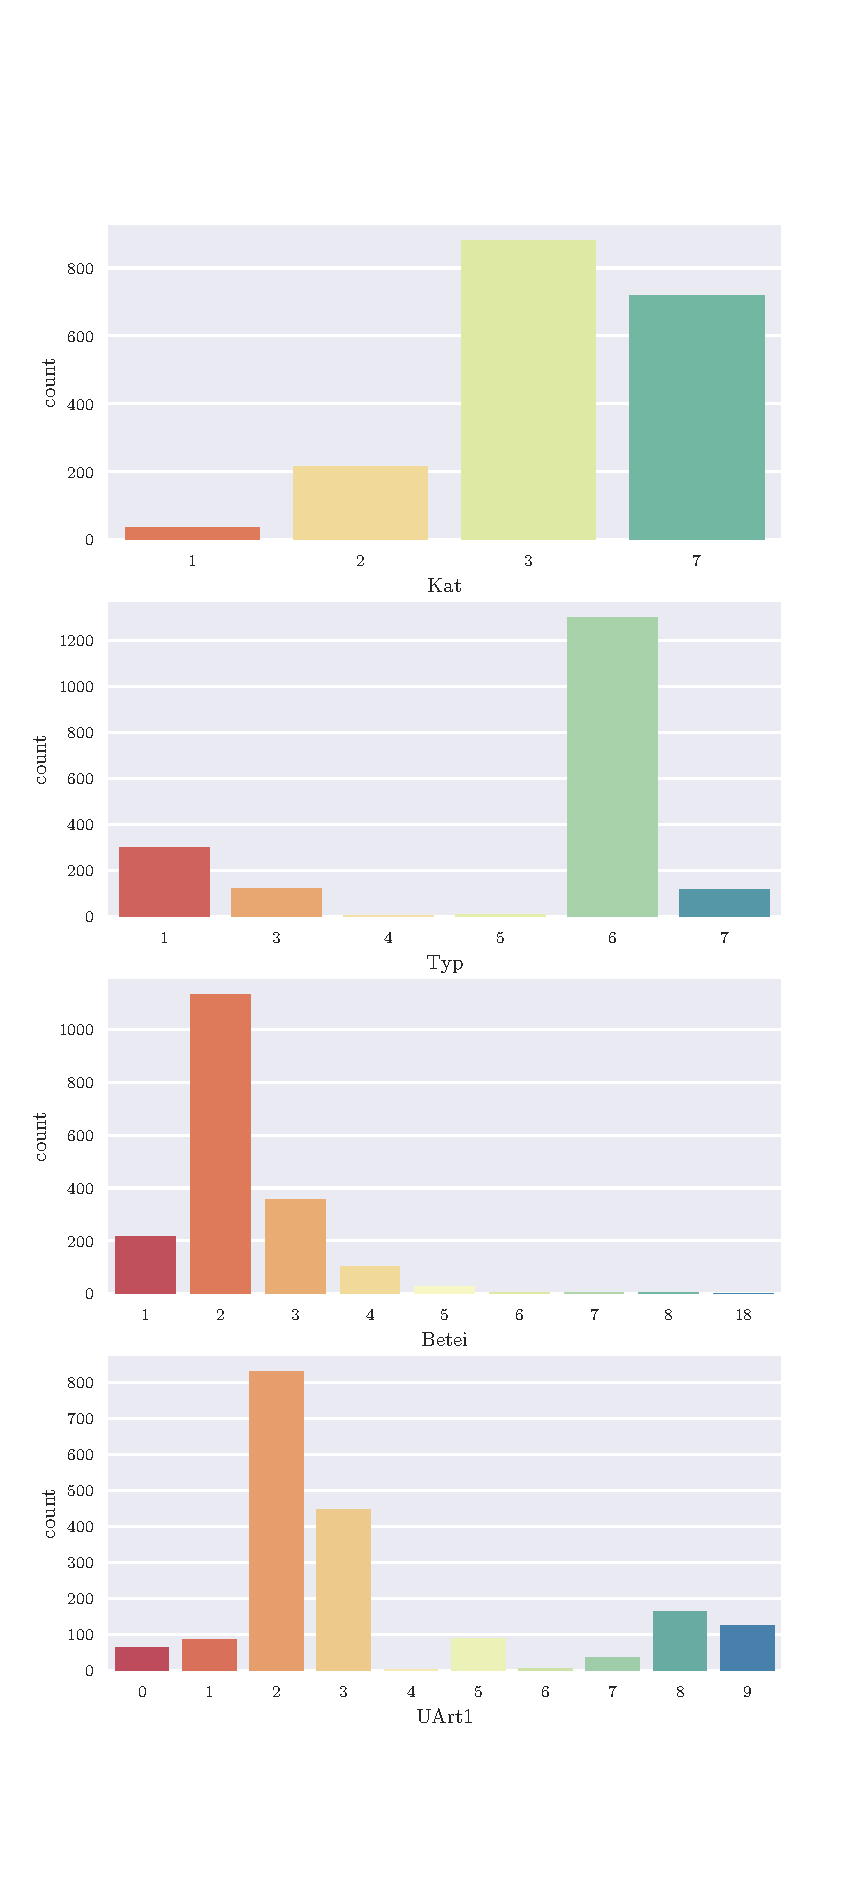
\includegraphics[scale=0.7]{CorrAnalysis/data/BAYSIS/02_matched/plots/baysis_matched_count_multiple01}
    %     \caption{Distribution of the accident category Kat, Typ, Betei and UArt}
    %     \label{img:baysis_matched_Kat}
    %     \label{img:baysis_matched_Typ}
    %     \label{img:baysis_matched_Betei}
    %     \label{img:baysis_matched_UArt}
    % \end{figure}

    % \begin{figure}[ht!]
    %     \centering
    %     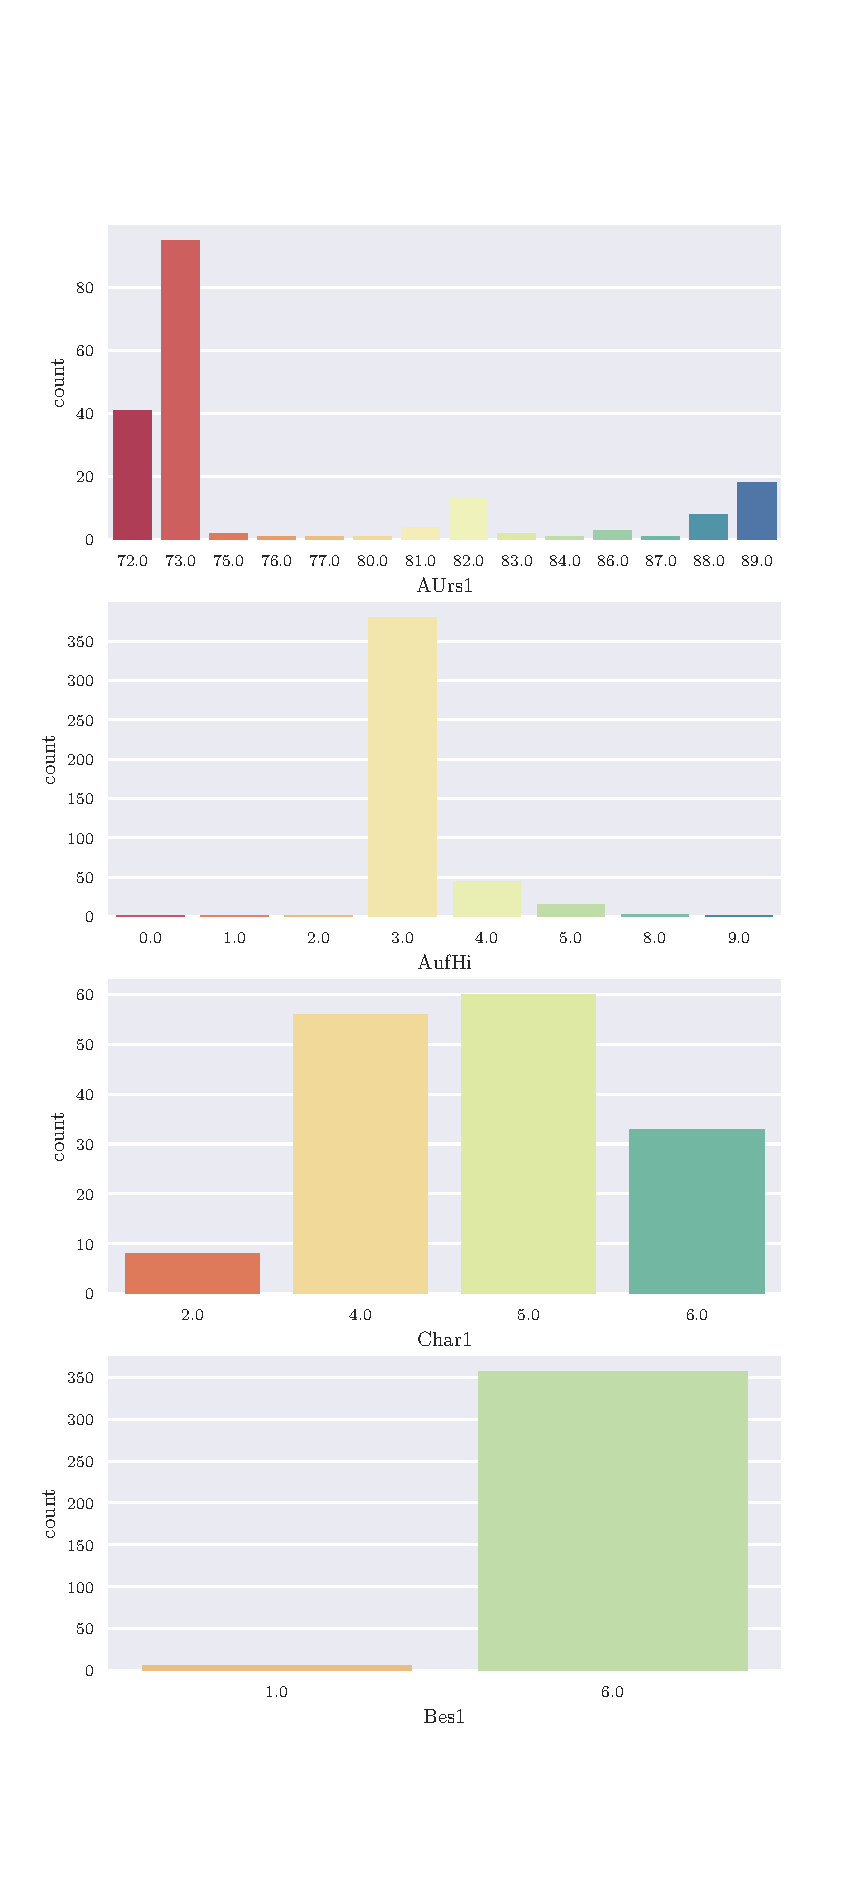
\includegraphics[scale=0.7]{CorrAnalysis/data/BAYSIS/02_matched/plots/baysis_matched_count_multiple02}
    %     \caption{Distribution of the accident category AUrs, AufHi, Char and Bes}
    %     \label{img:baysis_matched_AUrs}
    %     \label{img:baysis_matched_AufHi}
    %     \label{img:baysis_matched_Char}
    %     \label{img:baysis_matched_Bes}
    % \end{figure}

    % \begin{figure}[ht!]
    %     \centering
    %     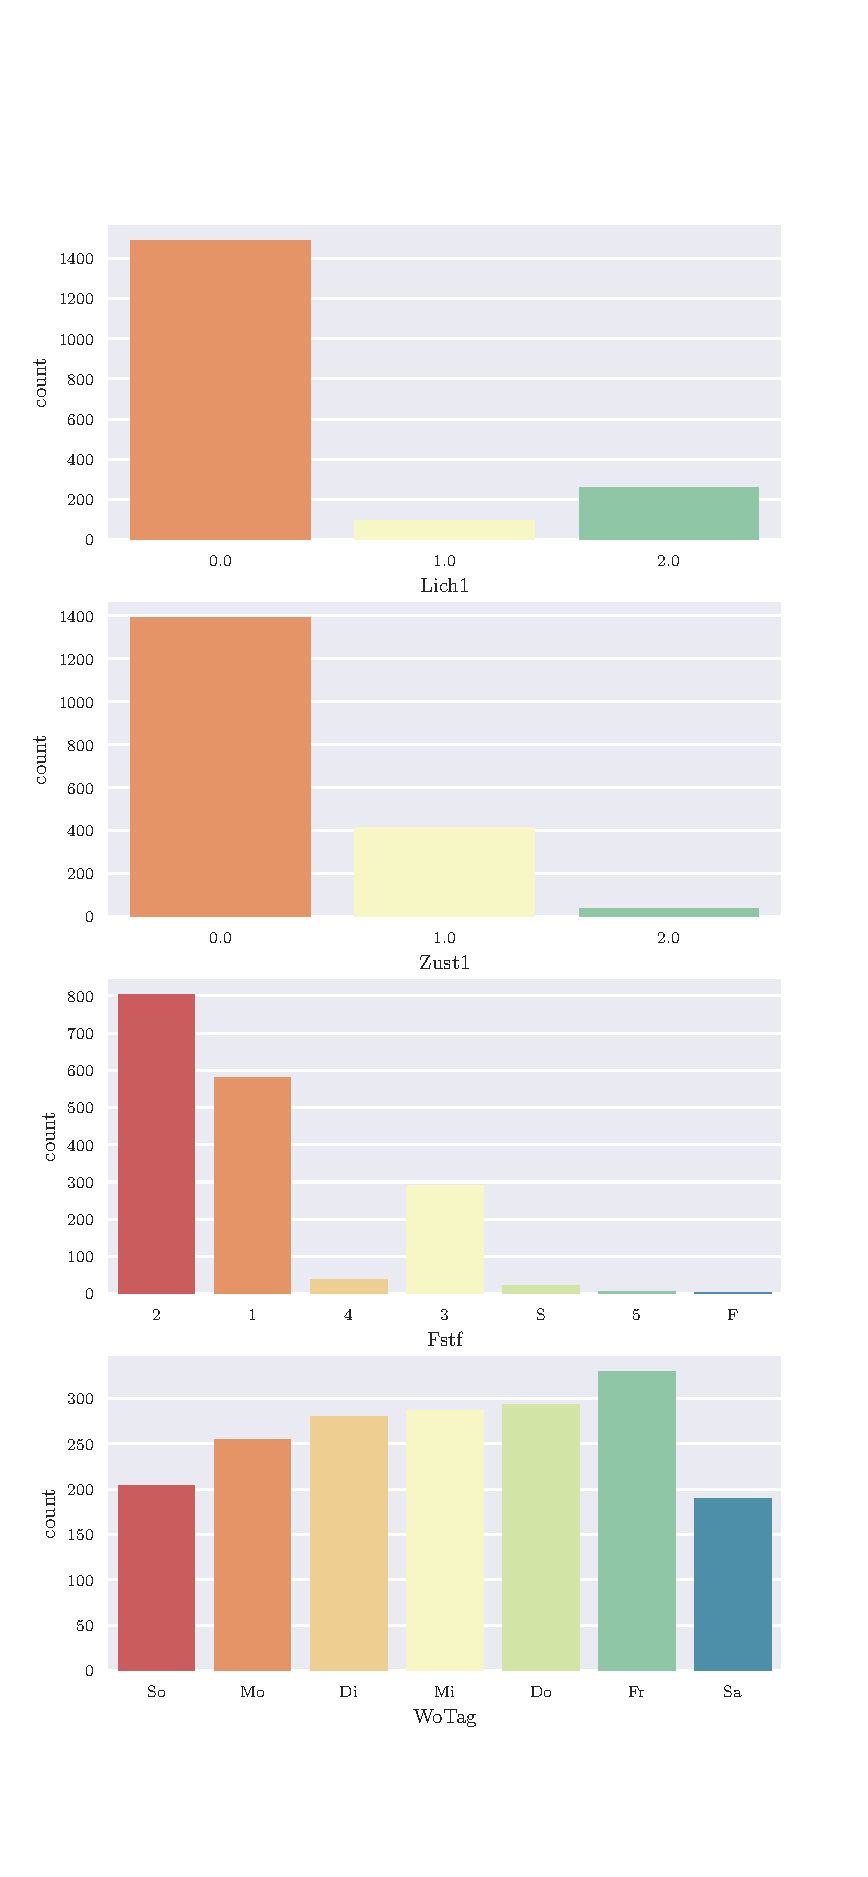
\includegraphics[scale=0.7]{CorrAnalysis/data/BAYSIS/02_matched/plots/baysis_matched_count_multiple03}
    %     \caption{Distribution of the accident category Lich, Zust, Fstf and WoTag}
    %     \label{img:baysis_matched_Lich}
    %     \label{img:baysis_matched_Zust}
    %     \label{img:baysis_matched_Fstf}
    %     \label{img:baysis_matched_WoTag}
    % \end{figure}
    
    % ------- BAYSIS Selected03 - Tables --------
    % \newgeometry{left=1cm,right=1cm,top=1cm}
    \begin{sidewaystable}
    	\tiny
    	\setlength{\tabcolsep}{2pt}
    	\centering
    	\begin{tabular}{lrrrrrrrrrrrrrrrrrrrrrrrrrrrrr}
\toprule
{} &  TMax &  TAvg &  SMax &  SAvg &  TDist &  SDist &   Cov &  TLCar &  TLHGV &  Str &  Kat &  Typ &  Betei &  UArt1 &  UArt2 &  AUrs1 &  AUrs2 &  AufHi &  Alkoh &  Char1 &  Char2 &  Lich1 &  Lich2 &  Zust1 &  Zust2 &  Fstf &  WoTag &  FeiTag &  Month \\
\midrule
TMax   &  1.00 &  0.81 &  0.49 &  0.50 &  -0.24 &  -0.05 & -0.12 &   0.05 &  -0.02 & 0.29 & 0.15 & 0.07 &   0.07 &   0.10 &   0.12 &   0.12 &   0.02 &   0.22 &   0.04 &   0.09 &   0.04 &   0.02 &   0.02 &   0.13 &   0.05 & -0.02 &   0.11 &   -0.00 &   0.19 \\
TAvg   &  0.81 &  1.00 &  0.19 &  0.45 &  -0.17 &  -0.03 &  0.24 &   0.01 &   0.01 & 0.22 & 0.13 & 0.12 &   0.08 &   0.16 &   0.07 &   0.07 &   0.01 &   0.33 &   0.04 &   0.05 &   0.03 &   0.10 &   0.08 &   0.09 &   0.04 & -0.02 &   0.15 &    0.00 &   0.15 \\
SMax   &  0.49 &  0.19 &  1.00 &  0.66 &  -0.21 &  -0.04 & -0.50 &   0.05 &  -0.10 & 0.35 & 0.18 & 0.10 &   0.07 &   0.17 &   0.09 &   0.10 &   0.02 &   0.11 &   0.03 &   0.07 &   0.04 &   0.08 &   0.06 &   0.09 &   0.04 &  0.05 &   0.15 &    0.05 &   0.21 \\
SAvg   &  0.50 &  0.45 &  0.66 &  1.00 &  -0.24 &  -0.11 &  0.09 &   0.01 &  -0.09 & 0.32 & 0.26 & 0.06 &   0.10 &   0.19 &   0.12 &   0.10 &   0.05 &   0.08 &   0.05 &   0.10 &   0.09 &   0.02 &   0.03 &   0.09 &   0.02 &  0.03 &   0.16 &    0.06 &   0.15 \\
TDist  & -0.24 & -0.17 & -0.21 & -0.24 &   1.00 &   0.08 &  0.03 &  -0.04 &   0.04 & 0.19 & 0.12 & 0.13 &  -0.09 &   0.24 &   0.15 &   0.20 &   0.02 &   0.07 &   0.02 &   0.09 &   0.08 &   0.01 &   0.03 &   0.10 &   0.05 &  0.01 &   0.15 &   -0.02 &   0.09 \\
SDist  & -0.05 & -0.03 & -0.04 & -0.11 &   0.08 &   1.00 &  0.00 &  -0.01 &   0.09 & 0.23 & 0.04 & 0.12 &  -0.03 &   0.12 &   0.10 &   0.17 &   0.02 &   0.07 &  -0.04 &   0.05 &   0.00 &   0.01 &   0.02 &   0.05 &   0.02 &  0.05 &   0.13 &    0.06 &   0.13 \\
Cov    & -0.12 &  0.24 & -0.50 &  0.09 &   0.03 &   0.00 &  1.00 &  -0.04 &   0.12 & 0.35 & 0.06 & 0.15 &   0.03 &   0.22 &   0.14 &   0.22 &   0.06 &   0.17 &  -0.01 &   0.08 &   0.05 &   0.15 &   0.14 &   0.14 &   0.02 & -0.01 &   0.18 &    0.01 &   0.23 \\
TLCar  &  0.05 &  0.01 &  0.05 &  0.01 &  -0.04 &  -0.01 & -0.04 &   1.00 &  -0.01 & 0.09 & 0.07 & 0.03 &   0.02 &   0.13 &   0.11 &   0.07 &   0.04 &   0.09 &  -0.02 &   0.12 &   0.01 &   0.09 &   0.09 &   0.07 &   0.04 & -0.01 &   0.14 &    0.03 &   0.11 \\
TLHGV  & -0.02 &  0.01 & -0.10 & -0.09 &   0.04 &   0.09 &  0.12 &  -0.01 &   1.00 & 0.24 & 0.06 & 0.11 &  -0.09 &   0.17 &   0.12 &   0.23 &   0.10 &   0.09 &  -0.05 &   0.11 &   0.05 &   0.06 &   0.05 &   0.12 &   0.00 & -0.01 &   0.20 &    0.03 &   0.18 \\
Str    &  0.29 &  0.22 &  0.35 &  0.32 &   0.19 &   0.23 &  0.35 &   0.09 &   0.24 & 1.00 & 0.15 & 0.23 &   0.15 &   0.20 &   0.14 &   0.24 &   0.14 &   0.17 &   0.12 &   0.23 &   0.41 &   0.23 &   0.17 &   0.25 &   0.16 &  0.20 &   0.18 &    0.13 &   0.19 \\
Kat    &  0.15 &  0.13 &  0.18 &  0.26 &   0.12 &   0.04 &  0.06 &   0.07 &   0.06 & 0.15 & 1.00 & 0.19 &   0.27 &   0.41 &   0.17 &   0.10 &   0.05 &   0.11 &   0.23 &   0.11 &   0.11 &   0.09 &   0.09 &   0.04 &   0.05 &  0.13 &   0.11 &    0.05 &   0.15 \\
Typ    &  0.07 &  0.12 &  0.10 &  0.06 &   0.13 &   0.12 &  0.15 &   0.03 &   0.11 & 0.23 & 0.19 & 1.00 &   0.36 &   0.52 &   0.13 &   0.30 &   0.09 &   0.32 &   0.07 &   0.10 &   0.25 &   0.13 &   0.24 &   0.20 &   0.13 &  0.24 &   0.14 &    0.10 &   0.18 \\
Betei  &  0.07 &  0.08 &  0.07 &  0.10 &  -0.09 &  -0.03 &  0.03 &   0.02 &  -0.09 & 0.15 & 0.27 & 0.36 &   1.00 &   0.33 &   0.20 &   0.20 &   0.03 &   0.37 &   0.06 &   0.11 &   0.26 &   0.13 &   0.11 &   0.17 &   0.07 &  0.17 &   0.12 &    0.07 &   0.17 \\
UArt1  &  0.10 &  0.16 &  0.17 &  0.19 &   0.24 &   0.12 &  0.22 &   0.13 &   0.17 & 0.20 & 0.41 & 0.52 &   0.33 &   1.00 &   0.33 &   0.32 &   0.15 &   0.51 &   0.13 &   0.13 &   0.23 &   0.14 &   0.15 &   0.19 &   0.12 &  0.21 &   0.14 &    0.11 &   0.17 \\
UArt2  &  0.12 &  0.07 &  0.09 &  0.12 &   0.15 &   0.10 &  0.14 &   0.11 &   0.12 & 0.14 & 0.17 & 0.13 &   0.20 &   0.33 &   1.00 &   0.12 &   0.01 &   0.42 &   0.03 &   0.08 &   0.13 &   0.09 &   0.07 &   0.11 &   0.03 &  0.12 &   0.13 &    0.06 &   0.16 \\
AUrs1  &  0.12 &  0.07 &  0.10 &  0.10 &   0.20 &   0.17 &  0.22 &   0.07 &   0.23 & 0.24 & 0.10 & 0.30 &   0.20 &   0.32 &   0.12 &   1.00 &   0.33 &   0.35 &   0.03 &   0.11 &   0.15 &   0.21 &   0.19 &   0.57 &   0.16 &  0.08 &   0.13 &    0.16 &   0.21 \\
AUrs2  &  0.02 &  0.01 &  0.02 &  0.05 &   0.02 &   0.02 &  0.06 &   0.04 &   0.10 & 0.14 & 0.05 & 0.09 &   0.03 &   0.15 &   0.01 &   0.33 &   1.00 &   0.02 &   0.01 &   0.01 &   0.01 &   0.16 &   0.08 &   0.33 &   0.01 &  0.06 &   0.11 &    0.01 &   0.18 \\
AufHi  &  0.22 &  0.33 &  0.11 &  0.08 &   0.07 &   0.07 &  0.17 &   0.09 &   0.09 & 0.17 & 0.11 & 0.32 &   0.37 &   0.51 &   0.42 &   0.35 &   0.02 &   1.00 &   0.05 &   0.12 &   0.30 &   0.07 &   0.08 &   0.16 &   0.04 &  0.18 &   0.14 &    0.18 &   0.16 \\
Alkoh  &  0.04 &  0.04 &  0.03 &  0.05 &   0.02 &  -0.04 & -0.01 &  -0.02 &  -0.05 & 0.12 & 0.23 & 0.07 &   0.06 &   0.13 &   0.03 &   0.03 &   0.01 &   0.05 &   1.00 &   0.03 &   0.07 &   0.08 &   0.01 &   0.06 &   0.09 &  0.09 &   0.07 &    0.05 &   0.13 \\
Char1  &  0.09 &  0.05 &  0.07 &  0.10 &   0.09 &   0.05 &  0.08 &   0.12 &   0.11 & 0.23 & 0.11 & 0.10 &   0.11 &   0.13 &   0.08 &   0.11 &   0.01 &   0.12 &   0.03 &   1.00 &   0.53 &   0.10 &   0.04 &   0.08 &   0.14 &  0.12 &   0.12 &    0.03 &   0.15 \\
Char2  &  0.04 &  0.03 &  0.04 &  0.09 &   0.08 &   0.00 &  0.05 &   0.01 &   0.05 & 0.41 & 0.11 & 0.25 &   0.26 &   0.23 &   0.13 &   0.15 &   0.01 &   0.30 &   0.07 &   0.53 &   1.00 &   0.08 &   0.06 &   0.13 &   0.09 &  0.21 &   0.07 &    0.05 &   0.15 \\
Lich1  &  0.02 &  0.10 &  0.08 &  0.02 &   0.01 &   0.01 &  0.15 &   0.09 &   0.06 & 0.23 & 0.09 & 0.13 &   0.13 &   0.14 &   0.09 &   0.21 &   0.16 &   0.07 &   0.08 &   0.10 &   0.08 &   1.00 &   0.71 &   0.19 &   0.10 &  0.11 &   0.22 &    0.05 &   0.34 \\
Lich2  &  0.02 &  0.08 &  0.06 &  0.03 &   0.03 &   0.02 &  0.14 &   0.09 &   0.05 & 0.17 & 0.09 & 0.24 &   0.11 &   0.15 &   0.07 &   0.19 &   0.08 &   0.08 &   0.01 &   0.04 &   0.06 &   0.71 &   1.00 &   0.19 &   0.03 &  0.12 &   0.19 &    0.03 &   0.33 \\
Zust1  &  0.13 &  0.09 &  0.09 &  0.09 &   0.10 &   0.05 &  0.14 &   0.07 &   0.12 & 0.25 & 0.04 & 0.20 &   0.17 &   0.19 &   0.11 &   0.57 &   0.33 &   0.16 &   0.06 &   0.08 &   0.13 &   0.19 &   0.19 &   1.00 &   0.19 &  0.08 &   0.17 &    0.10 &   0.30 \\
Zust2  &  0.05 &  0.04 &  0.04 &  0.02 &   0.05 &   0.02 &  0.02 &   0.04 &   0.00 & 0.16 & 0.05 & 0.13 &   0.07 &   0.12 &   0.03 &   0.16 &   0.01 &   0.04 &   0.09 &   0.14 &   0.09 &   0.10 &   0.03 &   0.19 &   1.00 &  0.10 &   0.08 &    0.07 &   0.25 \\
Fstf   & -0.02 & -0.02 &  0.05 &  0.03 &   0.01 &   0.05 & -0.01 &  -0.01 &  -0.01 & 0.20 & 0.13 & 0.24 &   0.17 &   0.21 &   0.12 &   0.08 &   0.06 &   0.18 &   0.09 &   0.12 &   0.21 &   0.11 &   0.12 &   0.08 &   0.10 &  1.00 &   0.11 &    0.13 &   0.14 \\
WoTag  &  0.11 &  0.15 &  0.15 &  0.16 &   0.15 &   0.13 &  0.18 &   0.14 &   0.20 & 0.18 & 0.11 & 0.14 &   0.12 &   0.14 &   0.13 &   0.13 &   0.11 &   0.14 &   0.07 &   0.12 &   0.07 &   0.22 &   0.19 &   0.17 &   0.08 &  0.11 &   1.00 &    0.16 &   0.18 \\
FeiTag & -0.00 &  0.00 &  0.05 &  0.06 &  -0.02 &   0.06 &  0.01 &   0.03 &   0.03 & 0.13 & 0.05 & 0.10 &   0.07 &   0.11 &   0.06 &   0.16 &   0.01 &   0.18 &   0.05 &   0.03 &   0.05 &   0.05 &   0.03 &   0.10 &   0.07 &  0.13 &   0.16 &    1.00 &   0.19 \\
Month  &  0.19 &  0.15 &  0.21 &  0.15 &   0.09 &   0.13 &  0.23 &   0.11 &   0.18 & 0.19 & 0.15 & 0.18 &   0.17 &   0.17 &   0.16 &   0.21 &   0.18 &   0.16 &   0.13 &   0.15 &   0.15 &   0.34 &   0.33 &   0.30 &   0.25 &  0.14 &   0.18 &    0.19 &   1.00 \\
\bottomrule
\end{tabular}

    	\caption{Correlation matrix for BAYSIS selected data (Jam Follower), calculated with Cramer's $V$, $\eta$, $\tau$, $r_{pq}$, $r$}
    	\label{table:appendix_correlation_matrix_selected_endJam_cramers}
    \end{sidewaystable}  
    \begin{sidewaystable}
    	\tiny
    	\setlength{\tabcolsep}{2pt}
    	\centering
    	\begin{tabular}{lrrrrrrrrrrrrrrrrrrrrrrrrrrrrr}
\toprule
{} &  TMax &  TAvg &  SMax &  SAvg &  TDist &  SDist &   Cov &  TLCar &  TLHGV &  Str &  Kat &  Typ &  Betei &  UArt1 &  UArt2 &  AUrs1 &  AUrs2 &  AufHi &  Alkoh &  Char1 &  Char2 &  Lich1 &  Lich2 &  Zust1 &  Zust2 &  Fstf &  WoTag &  FeiTag &  Month \\
\midrule
TMax   &  1.00 &  0.81 &  0.49 &  0.50 &  -0.24 &  -0.05 & -0.12 &   0.05 &  -0.02 & 0.29 & 0.15 & 0.07 &   0.07 &   0.10 &   0.12 &   0.12 &   0.02 &   0.22 &   0.04 &   0.09 &   0.04 &   0.02 &   0.02 &   0.13 &   0.05 & -0.02 &   0.11 &   -0.00 &   0.19 \\
TAvg   &  0.81 &  1.00 &  0.19 &  0.45 &  -0.17 &  -0.03 &  0.24 &   0.01 &   0.01 & 0.22 & 0.13 & 0.12 &   0.08 &   0.16 &   0.07 &   0.07 &   0.01 &   0.33 &   0.04 &   0.05 &   0.03 &   0.10 &   0.08 &   0.09 &   0.04 & -0.02 &   0.15 &    0.00 &   0.15 \\
SMax   &  0.49 &  0.19 &  1.00 &  0.66 &  -0.21 &  -0.04 & -0.50 &   0.05 &  -0.10 & 0.35 & 0.18 & 0.10 &   0.07 &   0.17 &   0.09 &   0.10 &   0.02 &   0.11 &   0.03 &   0.07 &   0.04 &   0.08 &   0.06 &   0.09 &   0.04 &  0.05 &   0.15 &    0.05 &   0.21 \\
SAvg   &  0.50 &  0.45 &  0.66 &  1.00 &  -0.24 &  -0.11 &  0.09 &   0.01 &  -0.09 & 0.32 & 0.26 & 0.06 &   0.10 &   0.19 &   0.12 &   0.10 &   0.05 &   0.08 &   0.05 &   0.10 &   0.09 &   0.02 &   0.03 &   0.09 &   0.02 &  0.03 &   0.16 &    0.06 &   0.15 \\
TDist  & -0.24 & -0.17 & -0.21 & -0.24 &   1.00 &   0.08 &  0.03 &  -0.04 &   0.04 & 0.19 & 0.12 & 0.13 &  -0.09 &   0.24 &   0.15 &   0.20 &   0.02 &   0.07 &   0.02 &   0.09 &   0.08 &   0.01 &   0.03 &   0.10 &   0.05 &  0.01 &   0.15 &   -0.02 &   0.09 \\
SDist  & -0.05 & -0.03 & -0.04 & -0.11 &   0.08 &   1.00 &  0.00 &  -0.01 &   0.09 & 0.23 & 0.04 & 0.12 &  -0.03 &   0.12 &   0.10 &   0.17 &   0.02 &   0.07 &  -0.04 &   0.05 &   0.00 &   0.01 &   0.02 &   0.05 &   0.02 &  0.05 &   0.13 &    0.06 &   0.13 \\
Cov    & -0.12 &  0.24 & -0.50 &  0.09 &   0.03 &   0.00 &  1.00 &  -0.04 &   0.12 & 0.35 & 0.06 & 0.15 &   0.03 &   0.22 &   0.14 &   0.22 &   0.06 &   0.17 &  -0.01 &   0.08 &   0.05 &   0.15 &   0.14 &   0.14 &   0.02 & -0.01 &   0.18 &    0.01 &   0.23 \\
TLCar  &  0.05 &  0.01 &  0.05 &  0.01 &  -0.04 &  -0.01 & -0.04 &   1.00 &  -0.01 & 0.09 & 0.07 & 0.03 &   0.02 &   0.13 &   0.11 &   0.07 &   0.04 &   0.09 &  -0.02 &   0.12 &   0.01 &   0.09 &   0.09 &   0.07 &   0.04 & -0.01 &   0.14 &    0.03 &   0.11 \\
TLHGV  & -0.02 &  0.01 & -0.10 & -0.09 &   0.04 &   0.09 &  0.12 &  -0.01 &   1.00 & 0.24 & 0.06 & 0.11 &  -0.09 &   0.17 &   0.12 &   0.23 &   0.10 &   0.09 &  -0.05 &   0.11 &   0.05 &   0.06 &   0.05 &   0.12 &   0.00 & -0.01 &   0.20 &    0.03 &   0.18 \\
Str    &  0.29 &  0.22 &  0.35 &  0.32 &   0.19 &   0.23 &  0.35 &   0.09 &   0.24 & 1.00 & 0.02 & 0.05 &   0.04 &   0.07 &   0.02 &   0.04 &   0.00 &   0.02 &   0.00 &   0.02 &   0.01 &   0.02 &   0.01 &   0.02 &   0.01 &  0.06 &   0.06 &    0.01 &   0.10 \\
Kat    &  0.15 &  0.13 &  0.18 &  0.26 &   0.12 &   0.04 &  0.06 &   0.07 &   0.06 & 0.05 & 1.00 & 0.08 &   0.14 &   0.31 &   0.04 &   0.02 &   0.00 &   0.02 &   0.01 &   0.02 &   0.01 &   0.01 &   0.01 &   0.00 &   0.00 &  0.03 &   0.02 &    0.00 &   0.04 \\
Typ    &  0.07 &  0.12 &  0.10 &  0.06 &   0.13 &   0.12 &  0.15 &   0.03 &   0.11 & 0.11 & 0.08 & 1.00 &   0.24 &   0.41 &   0.03 &   0.13 &   0.01 &   0.14 &   0.00 &   0.02 &   0.02 &   0.02 &   0.02 &   0.06 &   0.01 &  0.07 &   0.05 &    0.01 &   0.07 \\
Betei  &  0.07 &  0.08 &  0.07 &  0.10 &  -0.09 &  -0.03 &  0.03 &   0.02 &  -0.09 & 0.07 & 0.13 & 0.21 &   1.00 &   0.29 &   0.04 &   0.07 &   0.00 &   0.13 &   0.00 &   0.02 &   0.02 &   0.01 &   0.01 &   0.04 &   0.00 &  0.05 &   0.05 &    0.00 &   0.08 \\
UArt1  &  0.10 &  0.16 &  0.17 &  0.19 &   0.24 &   0.12 &  0.22 &   0.13 &   0.17 & 0.08 & 0.18 & 0.23 &   0.18 &   1.00 &   0.04 &   0.07 &   0.01 &   0.17 &   0.01 &   0.01 &   0.01 &   0.02 &   0.01 &   0.03 &   0.00 &  0.07 &   0.04 &    0.00 &   0.08 \\
UArt2  &  0.12 &  0.07 &  0.09 &  0.12 &   0.15 &   0.10 &  0.14 &   0.11 &   0.12 & 0.10 & 0.08 & 0.06 &   0.10 &   0.15 &   1.00 &   0.04 &   0.00 &   0.38 &   0.00 &   0.02 &   0.01 &   0.02 &   0.02 &   0.03 &   0.00 &  0.09 &   0.10 &    0.00 &   0.14 \\
AUrs1  &  0.12 &  0.07 &  0.10 &  0.10 &   0.20 &   0.17 &  0.22 &   0.07 &   0.23 & 0.18 & 0.04 & 0.30 &   0.19 &   0.29 &   0.05 &   1.00 &   0.05 &   0.24 &   0.00 &   0.03 &   0.01 &   0.07 &   0.07 &   0.41 &   0.01 &  0.07 &   0.12 &    0.02 &   0.24 \\
AUrs2  &  0.02 &  0.01 &  0.02 &  0.05 &   0.02 &   0.02 &  0.06 &   0.04 &   0.10 & 0.28 & 0.11 & 0.17 &   0.05 &   0.27 &   0.01 &   0.57 &   1.00 &   0.02 &   0.00 &   0.01 &   0.00 &   0.24 &   0.15 &   0.57 &   0.00 &  0.14 &   0.28 &    0.00 &   0.39 \\
AufHi  &  0.22 &  0.33 &  0.11 &  0.08 &   0.07 &   0.07 &  0.17 &   0.09 &   0.09 & 0.07 & 0.04 & 0.23 &   0.24 &   0.50 &   0.29 &   0.17 &   0.00 &   1.00 &   0.00 &   0.02 &   0.04 &   0.01 &   0.01 &   0.06 &   0.00 &  0.08 &   0.06 &    0.01 &   0.07 \\
Alkoh  &  0.04 &  0.04 &  0.03 &  0.05 &   0.02 &  -0.04 & -0.01 &  -0.02 &  -0.05 & 0.09 & 0.09 & 0.05 &   0.04 &   0.15 &   0.02 &   0.01 &   0.00 &   0.03 &   1.00 &   0.01 &   0.00 &   0.04 &   0.00 &   0.04 &   0.00 &  0.06 &   0.06 &    0.00 &   0.14 \\
Char1  &  0.09 &  0.05 &  0.07 &  0.10 &   0.09 &   0.05 &  0.08 &   0.12 &   0.11 & 0.16 & 0.05 & 0.05 &   0.06 &   0.07 &   0.03 &   0.04 &   0.00 &   0.04 &   0.00 &   1.00 &   0.17 &   0.03 &   0.01 &   0.03 &   0.01 &  0.07 &   0.09 &    0.00 &   0.14 \\
Char2  &  0.04 &  0.03 &  0.04 &  0.09 &   0.08 &   0.00 &  0.05 &   0.01 &   0.05 & 0.22 & 0.12 & 0.26 &   0.31 &   0.20 &   0.06 &   0.08 &   0.00 &   0.27 &   0.00 &   0.61 &   1.00 &   0.03 &   0.02 &   0.06 &   0.00 &  0.21 &   0.06 &    0.00 &   0.18 \\
Lich1  &  0.02 &  0.10 &  0.08 &  0.02 &   0.01 &   0.01 &  0.15 &   0.09 &   0.06 & 0.07 & 0.02 & 0.03 &   0.03 &   0.05 &   0.02 &   0.05 &   0.01 &   0.01 &   0.01 &   0.02 &   0.00 &   1.00 &   0.83 &   0.05 &   0.01 &  0.03 &   0.08 &    0.00 &   0.22 \\
Lich2  &  0.02 &  0.08 &  0.06 &  0.03 &   0.03 &   0.02 &  0.14 &   0.09 &   0.05 & 0.06 & 0.02 & 0.04 &   0.03 &   0.04 &   0.01 &   0.06 &   0.01 &   0.01 &   0.00 &   0.00 &   0.00 &   0.96 &   1.00 &   0.06 &   0.00 &  0.02 &   0.08 &    0.00 &   0.22 \\
Zust1  &  0.13 &  0.09 &  0.09 &  0.09 &   0.10 &   0.05 &  0.14 &   0.07 &   0.12 & 0.07 & 0.01 & 0.08 &   0.06 &   0.06 &   0.02 &   0.26 &   0.03 &   0.05 &   0.01 &   0.01 &   0.01 &   0.04 &   0.05 &   1.00 &   0.02 &  0.02 &   0.06 &    0.01 &   0.16 \\
Zust2  &  0.05 &  0.04 &  0.04 &  0.02 &   0.05 &   0.02 &  0.02 &   0.04 &   0.00 & 0.20 & 0.03 & 0.13 &   0.06 &   0.10 &   0.02 &   0.09 &   0.00 &   0.02 &   0.00 &   0.07 &   0.00 &   0.06 &   0.01 &   0.29 &   1.00 &  0.09 &   0.10 &    0.00 &   0.34 \\
Fstf   & -0.02 & -0.02 &  0.05 &  0.03 &   0.01 &   0.05 & -0.01 &  -0.01 &  -0.01 & 0.09 & 0.02 & 0.04 &   0.04 &   0.08 &   0.03 &   0.02 &   0.00 &   0.03 &   0.00 &   0.01 &   0.01 &   0.01 &   0.01 &   0.01 &   0.00 &  1.00 &   0.03 &    0.00 &   0.05 \\
WoTag  &  0.11 &  0.15 &  0.15 &  0.16 &   0.15 &   0.13 &  0.18 &   0.14 &   0.20 & 0.06 & 0.01 & 0.02 &   0.02 &   0.03 &   0.02 &   0.02 &   0.00 &   0.01 &   0.00 &   0.01 &   0.00 &   0.02 &   0.02 &   0.02 &   0.00 &  0.02 &   1.00 &    0.01 &   0.06 \\
FeiTag & -0.00 &  0.00 &  0.05 &  0.06 &  -0.02 &   0.06 &  0.01 &   0.03 &   0.03 & 0.10 & 0.02 & 0.05 &   0.03 &   0.06 &   0.02 &   0.07 &   0.00 &   0.05 &   0.00 &   0.01 &   0.00 &   0.02 &   0.00 &   0.03 &   0.00 &  0.04 &   0.14 &    1.00 &   0.19 \\
Month  &  0.19 &  0.15 &  0.21 &  0.15 &   0.09 &   0.13 &  0.23 &   0.11 &   0.18 & 0.08 & 0.02 & 0.03 &   0.03 &   0.05 &   0.02 &   0.04 &   0.00 &   0.02 &   0.00 &   0.02 &   0.01 &   0.05 &   0.04 &   0.04 &   0.01 &  0.02 &   0.05 &    0.01 &   1.00 \\
\bottomrule
\end{tabular}

    	\caption{Correlation matrix for BAYSIS selected data (Jam Follower), calculated with Theil's $U$, $\eta$, $\tau$, $r_{pq}$, $r$}
    	\label{table:appendix_correlation_matrix_selected_endJam_theils}
    \end{sidewaystable}
    \begin{sidewaystable}
    	\tiny
    	\setlength{\tabcolsep}{2pt}
    	\centering
    	\begin{tabular}{lrrrrrrrrrrrrrrrrrrrrrrrrrrrrr}
\toprule
{} &  TMax &  TAvg &  SMax &  SAvg &  TDist &  SDist &   Cov &  TLCar &  TLHGV &   Str &   Kat &   Typ &  Betei &  UArt1 &  UArt2 &  AUrs1 &  AUrs2 &  AufHi &  Alkoh &  Char1 &  Char2 &  Lich1 &  Lich2 &  Zust1 &  Zust2 &  Fstf &  WoTag &  FeiTag &  Month \\
\midrule
TMax   &   nan & 0.000 & 0.000 & 0.000 &  0.000 &  0.277 & 0.010 &  0.320 &  0.738 & 0.000 & 0.000 & 0.000 &  0.049 &  0.000 &  0.000 &  0.000 &  0.000 &  0.000 &  0.416 &  0.000 &  0.000 &  0.000 &  0.000 &  0.000 &  0.000 & 0.502 &  0.000 &   0.930 &  0.000 \\
TAvg   & 0.000 &   nan & 0.000 & 0.000 &  0.000 &  0.566 & 0.000 &  0.798 &  0.789 & 0.000 & 0.000 & 0.000 &  0.033 &  0.000 &  0.000 &  0.000 &  0.000 &  0.000 &  0.340 &  0.000 &  0.000 &  0.000 &  0.000 &  0.000 &  0.000 & 0.499 &  0.000 &   0.904 &  0.000 \\
SMax   & 0.000 & 0.000 &   nan & 0.000 &  0.000 &  0.378 & 0.000 &  0.314 &  0.038 & 0.000 & 0.000 & 0.000 &  0.057 &  0.000 &  0.000 &  0.000 &  0.000 &  0.000 &  0.514 &  0.000 &  0.000 &  0.000 &  0.000 &  0.000 &  0.000 & 0.126 &  0.000 &   0.189 &  0.000 \\
SAvg   & 0.000 & 0.000 & 0.000 &   nan &  0.000 &  0.021 & 0.046 &  0.810 &  0.061 & 0.000 & 0.000 & 0.000 &  0.005 &  0.000 &  0.000 &  0.000 &  0.000 &  0.000 &  0.321 &  0.000 &  0.000 &  0.000 &  0.000 &  0.000 &  0.000 & 0.342 &  0.000 &   0.125 &  0.000 \\
TDist  & 0.000 & 0.000 & 0.000 & 0.000 &    nan &  0.094 & 0.464 &  0.343 &  0.365 & 0.000 & 0.000 & 0.000 &  0.044 &  0.000 &  0.000 &  0.001 &  0.000 &  0.000 &  0.620 &  0.000 &  0.000 &  0.169 &  0.000 &  0.491 &  0.000 & 0.842 &  0.000 &   0.584 &  0.000 \\
SDist  & 0.277 & 0.566 & 0.378 & 0.021 &  0.094 &    nan & 0.971 &  0.870 &  0.043 & 0.000 & 0.000 & 0.000 &  0.517 &  0.000 &  0.000 &  0.000 &  0.000 &  0.000 &  0.392 &  0.000 &  0.000 &  0.001 &  0.000 &  0.191 &  0.000 & 0.226 &  0.000 &   0.195 &  0.000 \\
Cov    & 0.010 & 0.000 & 0.000 & 0.046 &  0.464 &  0.971 &   nan &  0.337 &  0.008 & 0.000 & 0.000 & 0.000 &  0.453 &  0.000 &  0.000 &  0.000 &  0.000 &  0.000 &  0.769 &  0.000 &  0.000 &  0.000 &  0.000 &  0.000 &  0.000 & 0.840 &  0.000 &   0.800 &  0.000 \\
TLCar  & 0.320 & 0.798 & 0.314 & 0.810 &  0.343 &  0.870 & 0.337 &    nan &  0.803 & 0.000 & 0.000 & 0.000 &  0.639 &  0.000 &  0.000 &  0.000 &  0.000 &  0.000 &  0.604 &  0.000 &  0.000 &  0.000 &  0.000 &  0.000 &  0.000 & 0.822 &  0.000 &   0.360 &  0.000 \\
TLHGV  & 0.738 & 0.789 & 0.038 & 0.061 &  0.365 &  0.043 & 0.008 &  0.803 &    nan & 0.000 & 0.000 & 0.000 &  0.017 &  0.000 &  0.000 &  0.000 &  0.000 &  0.000 &  0.300 &  0.000 &  0.000 &  0.000 &  0.000 &  0.000 &  0.000 & 0.886 &  0.000 &   0.419 &  0.000 \\
Str    & 0.000 & 0.000 & 0.000 & 0.000 &  0.000 &  0.000 & 0.000 &  0.000 &  0.000 &   nan & 0.507 & 0.000 &  0.696 &  0.000 &  0.772 &  0.000 &  0.616 &  0.128 &  0.817 &  0.000 &  0.000 &  0.001 &  0.207 &  0.000 &  0.390 & 0.000 &  0.037 &   0.738 &  0.001 \\
Kat    & 0.000 & 0.000 & 0.000 & 0.000 &  0.000 &  0.000 & 0.000 &  0.000 &  0.000 & 0.507 &   nan & 0.000 &  0.000 &  0.000 &  0.001 &  0.729 &  0.867 &  0.043 &  0.000 &  0.068 &  0.111 &  0.287 &  0.252 &  0.980 &  0.793 & 0.134 &  0.631 &   0.727 &  0.593 \\
Typ    & 0.000 & 0.000 & 0.000 & 0.000 &  0.000 &  0.000 & 0.000 &  0.000 &  0.000 & 0.000 & 0.000 &   nan &  0.000 &  0.000 &  0.194 &  0.000 &  0.455 &  0.000 &  0.731 &  0.365 &  0.000 &  0.068 &  0.000 &  0.000 &  0.099 & 0.000 &  0.107 &   0.377 &  0.067 \\
Betei  & 0.049 & 0.033 & 0.057 & 0.005 &  0.044 &  0.517 & 0.453 &  0.639 &  0.017 & 0.696 & 0.000 & 0.000 &    nan &  0.000 &  0.000 &  0.000 &  1.000 &  0.000 &  0.975 &  0.770 &  0.000 &  0.290 &  0.588 &  0.007 &  0.940 & 0.001 &  0.453 &   0.932 &  0.055 \\
UArt1  & 0.000 & 0.000 & 0.000 & 0.000 &  0.000 &  0.000 & 0.000 &  0.000 &  0.000 & 0.000 & 0.000 & 0.000 &  0.000 &    nan &  0.000 &  0.000 &  0.164 &  0.000 &  0.465 &  0.544 &  0.002 &  0.339 &  0.188 &  0.002 &  0.533 & 0.000 &  0.344 &   0.677 &  0.045 \\
UArt2  & 0.000 & 0.000 & 0.000 & 0.000 &  0.000 &  0.000 & 0.000 &  0.000 &  0.000 & 0.772 & 0.001 & 0.194 &  0.000 &  0.000 &    nan &  0.298 &  1.000 &  0.000 &  0.997 &  0.961 &  0.215 &  0.802 &  0.957 &  0.606 &  0.999 & 0.379 &  0.306 &   0.963 &  0.380 \\
AUrs1  & 0.000 & 0.000 & 0.000 & 0.000 &  0.001 &  0.000 & 0.000 &  0.000 &  0.000 & 0.000 & 0.729 & 0.000 &  0.000 &  0.000 &  0.298 &    nan &  0.000 &  0.000 &  0.998 &  0.525 &  0.107 &  0.000 &  0.001 &  0.000 &  0.076 & 0.988 &  0.312 &   0.055 &  0.000 \\
AUrs2  & 0.000 & 0.000 & 0.000 & 0.000 &  0.000 &  0.000 & 0.000 &  0.000 &  0.000 & 0.616 & 0.867 & 0.455 &  1.000 &  0.164 &  1.000 &  0.000 &    nan &  0.999 &  0.987 &  1.000 &  0.987 &  0.000 &  0.184 &  0.000 &  0.991 & 0.990 &  0.597 &   0.978 &  0.094 \\
AufHi  & 0.000 & 0.000 & 0.000 & 0.000 &  0.000 &  0.000 & 0.000 &  0.000 &  0.000 & 0.128 & 0.043 & 0.000 &  0.000 &  0.000 &  0.000 &  0.000 &  0.999 &    nan &  0.777 &  0.010 &  0.000 &  0.524 &  0.501 &  0.000 &  0.874 & 0.001 &  0.142 &   0.002 &  0.324 \\
Alkoh  & 0.416 & 0.340 & 0.514 & 0.321 &  0.620 &  0.392 & 0.769 &  0.604 &  0.300 & 0.817 & 0.000 & 0.731 &  0.975 &  0.465 &  0.997 &  0.998 &  0.987 &  0.777 &    nan &  0.954 &  0.124 &  0.224 &  0.973 &  0.653 &  0.046 & 0.712 &  0.940 &   0.294 &  0.702 \\
Char1  & 0.000 & 0.000 & 0.000 & 0.000 &  0.000 &  0.000 & 0.000 &  0.000 &  0.000 & 0.000 & 0.068 & 0.365 &  0.770 &  0.544 &  0.961 &  0.525 &  1.000 &  0.010 &  0.954 &    nan &  0.000 &  0.160 &  0.966 &  0.436 &  0.029 & 0.410 &  0.581 &   0.906 &  0.495 \\
Char2  & 0.000 & 0.000 & 0.000 & 0.000 &  0.000 &  0.000 & 0.000 &  0.000 &  0.000 & 0.000 & 0.111 & 0.000 &  0.000 &  0.002 &  0.215 &  0.107 &  0.987 &  0.000 &  0.124 &  0.000 &    nan &  0.245 &  0.400 &  0.044 &  0.046 & 0.003 &  0.920 &   0.294 &  0.464 \\
Lich1  & 0.000 & 0.000 & 0.000 & 0.000 &  0.169 &  0.001 & 0.000 &  0.000 &  0.000 & 0.001 & 0.287 & 0.068 &  0.290 &  0.339 &  0.802 &  0.000 &  0.000 &  0.524 &  0.224 &  0.160 &  0.245 &    nan &  0.000 &  0.000 &  0.091 & 0.563 &  0.000 &   0.518 &  0.000 \\
Lich2  & 0.000 & 0.000 & 0.000 & 0.000 &  0.000 &  0.000 & 0.000 &  0.000 &  0.000 & 0.207 & 0.252 & 0.000 &  0.588 &  0.188 &  0.957 &  0.001 &  0.184 &  0.501 &  0.973 &  0.966 &  0.400 &  0.000 &    nan &  0.000 &  0.820 & 0.382 &  0.001 &   0.853 &  0.000 \\
Zust1  & 0.000 & 0.000 & 0.000 & 0.000 &  0.491 &  0.191 & 0.000 &  0.000 &  0.000 & 0.000 & 0.980 & 0.000 &  0.007 &  0.002 &  0.606 &  0.000 &  0.000 &  0.000 &  0.653 &  0.436 &  0.044 &  0.000 &  0.000 &    nan &  0.001 & 0.967 &  0.007 &   0.207 &  0.000 \\
Zust2  & 0.000 & 0.000 & 0.000 & 0.000 &  0.000 &  0.000 & 0.000 &  0.000 &  0.000 & 0.390 & 0.793 & 0.099 &  0.940 &  0.533 &  0.999 &  0.076 &  0.991 &  0.874 &  0.046 &  0.029 &  0.046 &  0.091 &  0.820 &  0.001 &    nan & 0.592 &  0.852 &   0.152 &  0.002 \\
Fstf   & 0.502 & 0.499 & 0.126 & 0.342 &  0.842 &  0.226 & 0.840 &  0.822 &  0.886 & 0.000 & 0.134 & 0.000 &  0.001 &  0.000 &  0.379 &  0.988 &  0.990 &  0.001 &  0.712 &  0.410 &  0.003 &  0.563 &  0.382 &  0.967 &  0.592 &   nan &  0.850 &   0.281 &  0.819 \\
WoTag  & 0.000 & 0.000 & 0.000 & 0.000 &  0.000 &  0.000 & 0.000 &  0.000 &  0.000 & 0.037 & 0.631 & 0.107 &  0.453 &  0.344 &  0.306 &  0.312 &  0.597 &  0.142 &  0.940 &  0.581 &  0.920 &  0.000 &  0.001 &  0.007 &  0.852 & 0.850 &    nan &   0.100 &  0.011 \\
FeiTag & 0.930 & 0.904 & 0.189 & 0.125 &  0.584 &  0.195 & 0.800 &  0.360 &  0.419 & 0.738 & 0.727 & 0.377 &  0.932 &  0.677 &  0.963 &  0.055 &  0.978 &  0.002 &  0.294 &  0.906 &  0.294 &  0.518 &  0.853 &  0.207 &  0.152 & 0.281 &  0.100 &     nan &  0.092 \\
Month  & 0.000 & 0.000 & 0.000 & 0.000 &  0.000 &  0.000 & 0.000 &  0.000 &  0.000 & 0.001 & 0.593 & 0.067 &  0.055 &  0.045 &  0.380 &  0.000 &  0.094 &  0.324 &  0.702 &  0.495 &  0.464 &  0.000 &  0.000 &  0.000 &  0.002 & 0.819 &  0.011 &   0.092 &    nan \\
\bottomrule
\end{tabular}

    	\caption{Significancy matrix for BAYSIS selected data (Jam Follower)}
    	\label{table:appendix_significancy_matrix_selected_endJam}
    \end{sidewaystable}
    \begin{sidewaystable}
    	\tiny
    	\setlength{\tabcolsep}{2pt}
    	\centering
    	\begin{tabular}{llllllllllllllllllllllllllllll}
\toprule
{} &      TMax &      TAvg &      SMax &      SAvg &     TDist &     SDist &       Cov &     TLCar &     TLHGV &     Str &     Kat &     Typ &   Betei &   UArt1 &   UArt2 &   AUrs1 &   AUrs2 &   AufHi &     Alkoh &   Char1 &   Char2 &   Lich1 &   Lich2 &   Zust1 &   Zust2 &    Fstf &   WoTag &  FeiTag &   Month \\
\midrule
TMax   &       NaN &       $r$ &       $r$ &       $r$ &       $r$ &       $r$ &       $r$ &       $r$ &       $r$ &  $\eta$ &  $\eta$ &  $\eta$ &  $\tau$ &  $\eta$ &  $\eta$ &  $\eta$ &  $\eta$ &  $\eta$ &  $r_{pq}$ &  $\eta$ &  $\eta$ &  $\eta$ &  $\eta$ &  $\eta$ &  $\eta$ &  $\tau$ &  $\eta$ &  $\tau$ &  $\eta$ \\
TAvg   &       $r$ &       NaN &       $r$ &       $r$ &       $r$ &       $r$ &       $r$ &       $r$ &       $r$ &  $\eta$ &  $\eta$ &  $\eta$ &  $\tau$ &  $\eta$ &  $\eta$ &  $\eta$ &  $\eta$ &  $\eta$ &  $r_{pq}$ &  $\eta$ &  $\eta$ &  $\eta$ &  $\eta$ &  $\eta$ &  $\eta$ &  $\tau$ &  $\eta$ &  $\tau$ &  $\eta$ \\
SMax   &       $r$ &       $r$ &       NaN &       $r$ &       $r$ &       $r$ &       $r$ &       $r$ &       $r$ &  $\eta$ &  $\eta$ &  $\eta$ &  $\tau$ &  $\eta$ &  $\eta$ &  $\eta$ &  $\eta$ &  $\eta$ &  $r_{pq}$ &  $\eta$ &  $\eta$ &  $\eta$ &  $\eta$ &  $\eta$ &  $\eta$ &  $\tau$ &  $\eta$ &  $\tau$ &  $\eta$ \\
SAvg   &       $r$ &       $r$ &       $r$ &       NaN &       $r$ &       $r$ &       $r$ &       $r$ &       $r$ &  $\eta$ &  $\eta$ &  $\eta$ &  $\tau$ &  $\eta$ &  $\eta$ &  $\eta$ &  $\eta$ &  $\eta$ &  $r_{pq}$ &  $\eta$ &  $\eta$ &  $\eta$ &  $\eta$ &  $\eta$ &  $\eta$ &  $\tau$ &  $\eta$ &  $\tau$ &  $\eta$ \\
TDist  &       $r$ &       $r$ &       $r$ &       $r$ &       NaN &       $r$ &       $r$ &       $r$ &       $r$ &  $\eta$ &  $\eta$ &  $\eta$ &  $\tau$ &  $\eta$ &  $\eta$ &  $\eta$ &  $\eta$ &  $\eta$ &  $r_{pq}$ &  $\eta$ &  $\eta$ &  $\eta$ &  $\eta$ &  $\eta$ &  $\eta$ &  $\tau$ &  $\eta$ &  $\tau$ &  $\eta$ \\
SDist  &       $r$ &       $r$ &       $r$ &       $r$ &       $r$ &       NaN &       $r$ &       $r$ &       $r$ &  $\eta$ &  $\eta$ &  $\eta$ &  $\tau$ &  $\eta$ &  $\eta$ &  $\eta$ &  $\eta$ &  $\eta$ &  $r_{pq}$ &  $\eta$ &  $\eta$ &  $\eta$ &  $\eta$ &  $\eta$ &  $\eta$ &  $\tau$ &  $\eta$ &  $\tau$ &  $\eta$ \\
Cov    &       $r$ &       $r$ &       $r$ &       $r$ &       $r$ &       $r$ &       NaN &       $r$ &       $r$ &  $\eta$ &  $\eta$ &  $\eta$ &  $\tau$ &  $\eta$ &  $\eta$ &  $\eta$ &  $\eta$ &  $\eta$ &  $r_{pq}$ &  $\eta$ &  $\eta$ &  $\eta$ &  $\eta$ &  $\eta$ &  $\eta$ &  $\tau$ &  $\eta$ &  $\tau$ &  $\eta$ \\
TLCar  &       $r$ &       $r$ &       $r$ &       $r$ &       $r$ &       $r$ &       $r$ &       NaN &       $r$ &  $\eta$ &  $\eta$ &  $\eta$ &  $\tau$ &  $\eta$ &  $\eta$ &  $\eta$ &  $\eta$ &  $\eta$ &  $r_{pq}$ &  $\eta$ &  $\eta$ &  $\eta$ &  $\eta$ &  $\eta$ &  $\eta$ &  $\tau$ &  $\eta$ &  $\tau$ &  $\eta$ \\
TLHGV  &       $r$ &       $r$ &       $r$ &       $r$ &       $r$ &       $r$ &       $r$ &       $r$ &       NaN &  $\eta$ &  $\eta$ &  $\eta$ &  $\tau$ &  $\eta$ &  $\eta$ &  $\eta$ &  $\eta$ &  $\eta$ &  $r_{pq}$ &  $\eta$ &  $\eta$ &  $\eta$ &  $\eta$ &  $\eta$ &  $\eta$ &  $\tau$ &  $\eta$ &  $\tau$ &  $\eta$ \\
Str    &    $\eta$ &    $\eta$ &    $\eta$ &    $\eta$ &    $\eta$ &    $\eta$ &    $\eta$ &    $\eta$ &    $\eta$ &     NaN &     $V$ &     $V$ &     $V$ &     $V$ &     $V$ &     $V$ &     $V$ &     $V$ &       $V$ &     $V$ &     $V$ &     $V$ &     $V$ &     $V$ &     $V$ &     $V$ &     $V$ &     $V$ &     $V$ \\
Kat    &    $\eta$ &    $\eta$ &    $\eta$ &    $\eta$ &    $\eta$ &    $\eta$ &    $\eta$ &    $\eta$ &    $\eta$ &     $V$ &     NaN &     $V$ &     $V$ &     $V$ &     $V$ &     $V$ &     $V$ &     $V$ &       $V$ &     $V$ &     $V$ &     $V$ &     $V$ &     $V$ &     $V$ &     $V$ &     $V$ &     $V$ &     $V$ \\
Typ    &    $\eta$ &    $\eta$ &    $\eta$ &    $\eta$ &    $\eta$ &    $\eta$ &    $\eta$ &    $\eta$ &    $\eta$ &     $V$ &     $V$ &     NaN &     $V$ &     $V$ &     $V$ &     $V$ &     $V$ &     $V$ &       $V$ &     $V$ &     $V$ &     $V$ &     $V$ &     $V$ &     $V$ &     $V$ &     $V$ &     $V$ &     $V$ \\
Betei  &    $\tau$ &    $\tau$ &    $\tau$ &    $\tau$ &    $\tau$ &    $\tau$ &    $\tau$ &    $\tau$ &    $\tau$ &     $V$ &     $V$ &     $V$ &     NaN &     $V$ &     $V$ &     $V$ &     $V$ &     $V$ &       $V$ &     $V$ &     $V$ &     $V$ &     $V$ &     $V$ &     $V$ &     $V$ &     $V$ &     $V$ &     $V$ \\
UArt1  &    $\eta$ &    $\eta$ &    $\eta$ &    $\eta$ &    $\eta$ &    $\eta$ &    $\eta$ &    $\eta$ &    $\eta$ &     $V$ &     $V$ &     $V$ &     $V$ &     NaN &     $V$ &     $V$ &     $V$ &     $V$ &       $V$ &     $V$ &     $V$ &     $V$ &     $V$ &     $V$ &     $V$ &     $V$ &     $V$ &     $V$ &     $V$ \\
UArt2  &    $\eta$ &    $\eta$ &    $\eta$ &    $\eta$ &    $\eta$ &    $\eta$ &    $\eta$ &    $\eta$ &    $\eta$ &     $V$ &     $V$ &     $V$ &     $V$ &     $V$ &     NaN &     $V$ &     $V$ &     $V$ &       $V$ &     $V$ &     $V$ &     $V$ &     $V$ &     $V$ &     $V$ &     $V$ &     $V$ &     $V$ &     $V$ \\
AUrs1  &    $\eta$ &    $\eta$ &    $\eta$ &    $\eta$ &    $\eta$ &    $\eta$ &    $\eta$ &    $\eta$ &    $\eta$ &     $V$ &     $V$ &     $V$ &     $V$ &     $V$ &     $V$ &     NaN &     $V$ &     $V$ &       $V$ &     $V$ &     $V$ &     $V$ &     $V$ &     $V$ &     $V$ &     $V$ &     $V$ &     $V$ &     $V$ \\
AUrs2  &    $\eta$ &    $\eta$ &    $\eta$ &    $\eta$ &    $\eta$ &    $\eta$ &    $\eta$ &    $\eta$ &    $\eta$ &     $V$ &     $V$ &     $V$ &     $V$ &     $V$ &     $V$ &     $V$ &     NaN &     $V$ &       $V$ &     $V$ &     $V$ &     $V$ &     $V$ &     $V$ &     $V$ &     $V$ &     $V$ &     $V$ &     $V$ \\
AufHi  &    $\eta$ &    $\eta$ &    $\eta$ &    $\eta$ &    $\eta$ &    $\eta$ &    $\eta$ &    $\eta$ &    $\eta$ &     $V$ &     $V$ &     $V$ &     $V$ &     $V$ &     $V$ &     $V$ &     $V$ &     NaN &       $V$ &     $V$ &     $V$ &     $V$ &     $V$ &     $V$ &     $V$ &     $V$ &     $V$ &     $V$ &     $V$ \\
Alkoh  &  $r_{pq}$ &  $r_{pq}$ &  $r_{pq}$ &  $r_{pq}$ &  $r_{pq}$ &  $r_{pq}$ &  $r_{pq}$ &  $r_{pq}$ &  $r_{pq}$ &     $V$ &     $V$ &     $V$ &     $V$ &     $V$ &     $V$ &     $V$ &     $V$ &     $V$ &       NaN &     $V$ &     $V$ &     $V$ &     $V$ &     $V$ &     $V$ &     $V$ &     $V$ &     $V$ &     $V$ \\
Char1  &    $\eta$ &    $\eta$ &    $\eta$ &    $\eta$ &    $\eta$ &    $\eta$ &    $\eta$ &    $\eta$ &    $\eta$ &     $V$ &     $V$ &     $V$ &     $V$ &     $V$ &     $V$ &     $V$ &     $V$ &     $V$ &       $V$ &     NaN &     $V$ &     $V$ &     $V$ &     $V$ &     $V$ &     $V$ &     $V$ &     $V$ &     $V$ \\
Char2  &    $\eta$ &    $\eta$ &    $\eta$ &    $\eta$ &    $\eta$ &    $\eta$ &    $\eta$ &    $\eta$ &    $\eta$ &     $V$ &     $V$ &     $V$ &     $V$ &     $V$ &     $V$ &     $V$ &     $V$ &     $V$ &       $V$ &     $V$ &     NaN &     $V$ &     $V$ &     $V$ &     $V$ &     $V$ &     $V$ &     $V$ &     $V$ \\
Lich1  &    $\eta$ &    $\eta$ &    $\eta$ &    $\eta$ &    $\eta$ &    $\eta$ &    $\eta$ &    $\eta$ &    $\eta$ &     $V$ &     $V$ &     $V$ &     $V$ &     $V$ &     $V$ &     $V$ &     $V$ &     $V$ &       $V$ &     $V$ &     $V$ &     NaN &     $V$ &     $V$ &     $V$ &     $V$ &     $V$ &     $V$ &     $V$ \\
Lich2  &    $\eta$ &    $\eta$ &    $\eta$ &    $\eta$ &    $\eta$ &    $\eta$ &    $\eta$ &    $\eta$ &    $\eta$ &     $V$ &     $V$ &     $V$ &     $V$ &     $V$ &     $V$ &     $V$ &     $V$ &     $V$ &       $V$ &     $V$ &     $V$ &     $V$ &     NaN &     $V$ &     $V$ &     $V$ &     $V$ &     $V$ &     $V$ \\
Zust1  &    $\eta$ &    $\eta$ &    $\eta$ &    $\eta$ &    $\eta$ &    $\eta$ &    $\eta$ &    $\eta$ &    $\eta$ &     $V$ &     $V$ &     $V$ &     $V$ &     $V$ &     $V$ &     $V$ &     $V$ &     $V$ &       $V$ &     $V$ &     $V$ &     $V$ &     $V$ &     NaN &     $V$ &     $V$ &     $V$ &     $V$ &     $V$ \\
Zust2  &    $\eta$ &    $\eta$ &    $\eta$ &    $\eta$ &    $\eta$ &    $\eta$ &    $\eta$ &    $\eta$ &    $\eta$ &     $V$ &     $V$ &     $V$ &     $V$ &     $V$ &     $V$ &     $V$ &     $V$ &     $V$ &       $V$ &     $V$ &     $V$ &     $V$ &     $V$ &     $V$ &     NaN &     $V$ &     $V$ &     $V$ &     $V$ \\
Fstf   &    $\tau$ &    $\tau$ &    $\tau$ &    $\tau$ &    $\tau$ &    $\tau$ &    $\tau$ &    $\tau$ &    $\tau$ &     $V$ &     $V$ &     $V$ &     $V$ &     $V$ &     $V$ &     $V$ &     $V$ &     $V$ &       $V$ &     $V$ &     $V$ &     $V$ &     $V$ &     $V$ &     $V$ &     NaN &     $V$ &     $V$ &     $V$ \\
WoTag  &    $\eta$ &    $\eta$ &    $\eta$ &    $\eta$ &    $\eta$ &    $\eta$ &    $\eta$ &    $\eta$ &    $\eta$ &     $V$ &     $V$ &     $V$ &     $V$ &     $V$ &     $V$ &     $V$ &     $V$ &     $V$ &       $V$ &     $V$ &     $V$ &     $V$ &     $V$ &     $V$ &     $V$ &     $V$ &     NaN &     $V$ &     $V$ \\
FeiTag &    $\tau$ &    $\tau$ &    $\tau$ &    $\tau$ &    $\tau$ &    $\tau$ &    $\tau$ &    $\tau$ &    $\tau$ &     $V$ &     $V$ &     $V$ &     $V$ &     $V$ &     $V$ &     $V$ &     $V$ &     $V$ &       $V$ &     $V$ &     $V$ &     $V$ &     $V$ &     $V$ &     $V$ &     $V$ &     $V$ &     NaN &     $V$ \\
Month  &    $\eta$ &    $\eta$ &    $\eta$ &    $\eta$ &    $\eta$ &    $\eta$ &    $\eta$ &    $\eta$ &    $\eta$ &     $V$ &     $V$ &     $V$ &     $V$ &     $V$ &     $V$ &     $V$ &     $V$ &     $V$ &       $V$ &     $V$ &     $V$ &     $V$ &     $V$ &     $V$ &     $V$ &     $V$ &     $V$ &     $V$ &     NaN \\
\bottomrule
\end{tabular}

    	\caption{Coefficient matrix for BAYSIS selected data (Jam Follower)}
    	\label{table:appendix_coefficient_matrix_selected_endJam}
    \end{sidewaystable}
    % \restoregeometry

    % -------------------------------
    % -------------------------------
    % ------- ArbIS Appendix --------
    % -------------------------------
    % -------------------------------
    \chapter{ArbIS Figures, Tables and Listings}
    \label{appendix_arbis}
    % -------------------------------
    % ------- ArbIS Dataset ---------
    % -------------------------------
    % \tocless\section{ArbIS Data Foundation}
    % \label{appendix_arbis_dataset}

    % ------- ArbIS Dataset - Figures --------
    \begin{figure}[ht!]
        \centering
        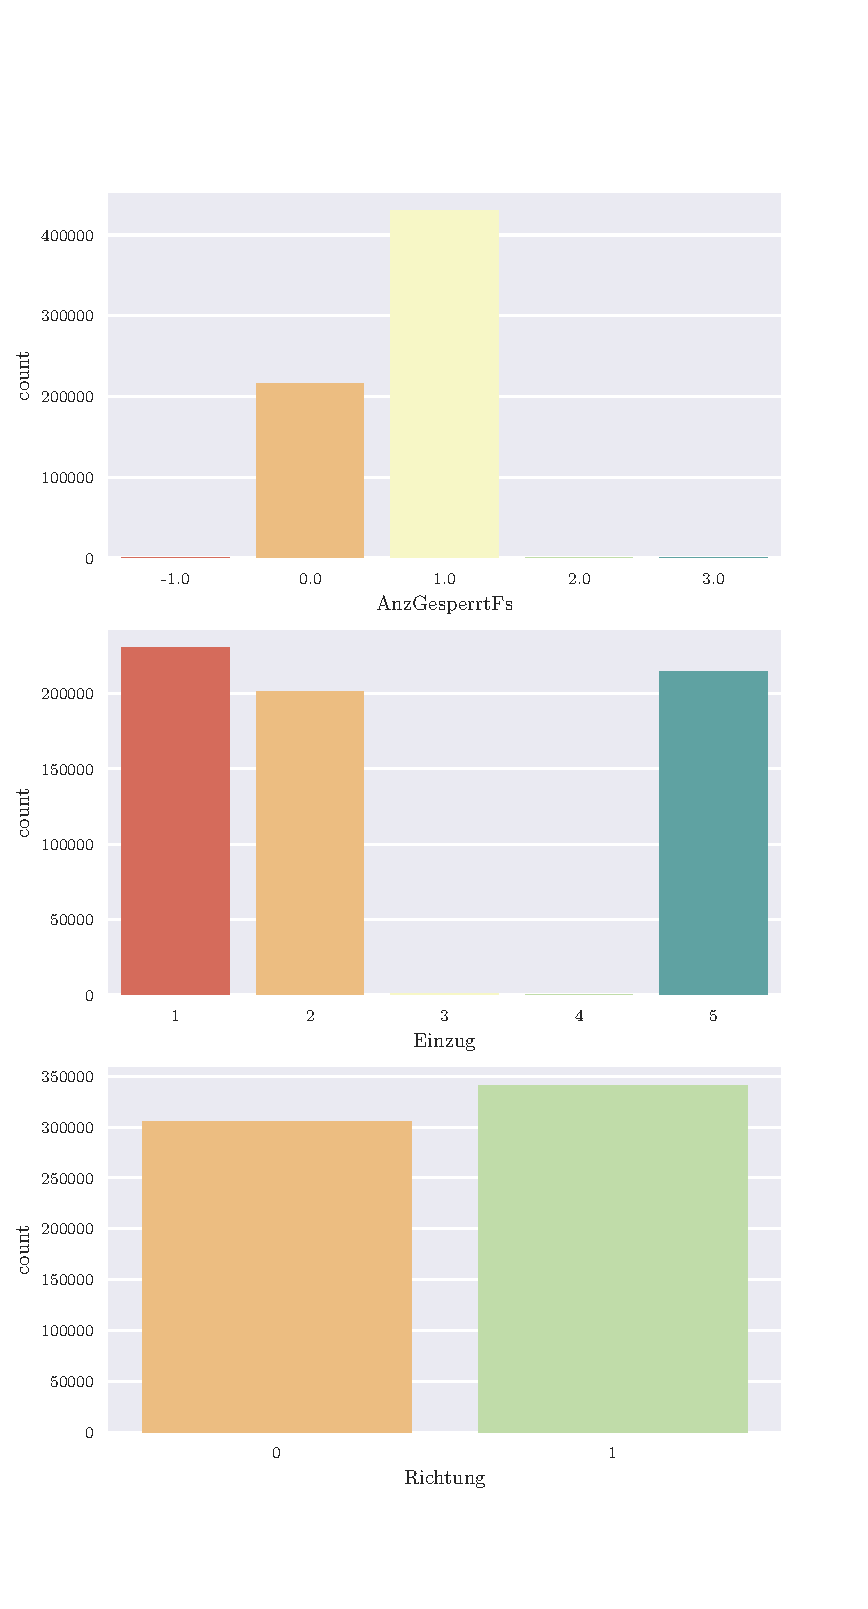
\includegraphics[scale=0.7]{CorrAnalysis/data/ArbIS/01_dataset/plots/arbis_dataset_count_multiple01}
        \caption{Distribution of the accident category \textit{AnzGesperrtFs}, \textit{Einzug} and \textit{Richtung}}
        \label{img:arbis_dataset_AnzGesperrtFs}
        \label{img:arbis_dataset_Einzug}
        \label{img:arbis_dataset_Richtung}
    \end{figure}

    \begin{figure}[ht!]
        \centering
        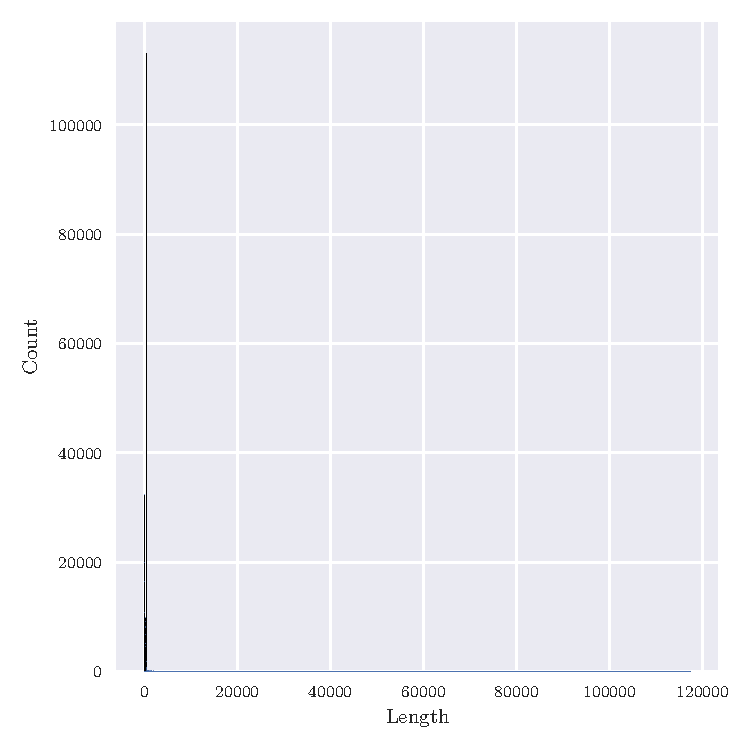
\includegraphics[scale=0.7]{CorrAnalysis/data/ArbIS/01_dataset/plots/arbis_dataset_dist_Length}
        \caption{Distribution of the roadwork parameter \textit{Length}}
        \label{img:arbis_matched_Length}
    \end{figure}

    \begin{figure}[ht!]
        \centering
        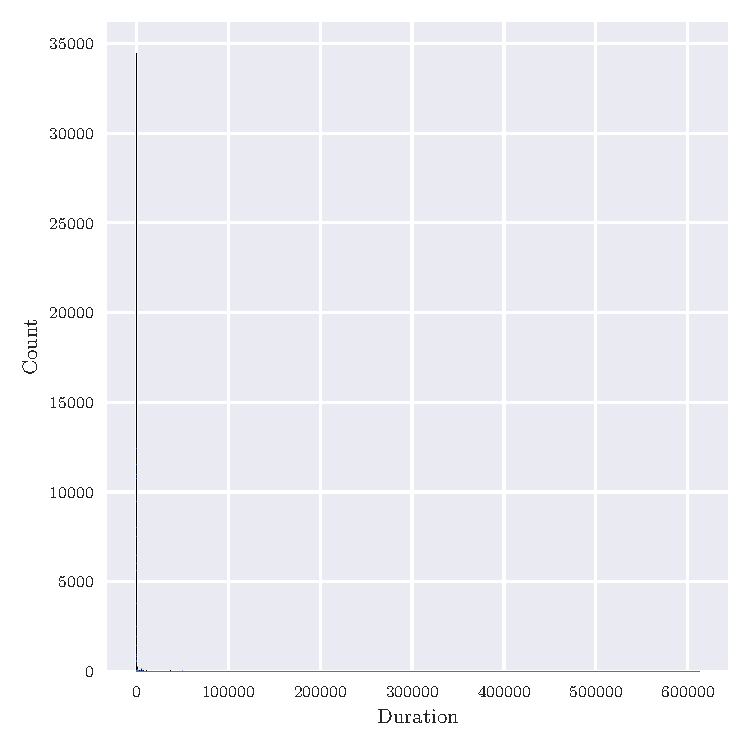
\includegraphics[scale=0.7]{CorrAnalysis/data/ArbIS/01_dataset/plots/arbis_dataset_dist_Duration}
        \caption{Distribution of the roadwork parameter \textit{Duration}}
        \label{img:arbis_matched_Duration}
    \end{figure}

    % ------- ArbIS Dataset - Tables --------
    % \newgeometry{left=1cm,right=1cm}
    \begin{table}
        \setlength{\tabcolsep}{4pt}
        \centering
        \begin{tabular}{lrrrrrrr}
\toprule
{} &  Strasse &  AnzGesperrtFs &  Einzug &  Richtung &  Length &  Duration &  Month \\
\midrule
Strasse       &     1.00 &           0.16 &    0.17 &      0.05 &    0.04 &      0.02 &   0.06 \\
AnzGesperrtFs &     0.16 &           1.00 &    0.50 &      0.00 &    0.02 &      0.11 &   0.06 \\
Einzug        &     0.17 &           0.50 &    1.00 &      0.02 &   -0.00 &     -0.15 &   0.11 \\
Richtung      &     0.05 &           0.00 &    0.02 &      1.00 &   -0.02 &     -0.00 &   0.03 \\
Length        &     0.04 &           0.02 &   -0.00 &     -0.02 &    1.00 &      0.08 &   0.04 \\
Duration      &     0.02 &           0.11 &   -0.15 &     -0.00 &    0.08 &      1.00 &   0.02 \\
Month         &     0.06 &           0.06 &    0.11 &      0.03 &    0.04 &      0.02 &   1.00 \\
\bottomrule
\end{tabular}

        \caption{Correlation matrix for ArbIS dataset, calculated with Cramer's $V$, $\eta$, $\tau$, $r_{pq}$, $r$}
        \label{tbl:appendix_arbis_correlation_matrix_dataset_cramers}
    \end{table}
    \begin{table}
        \setlength{\tabcolsep}{4pt}
        \centering
        \begin{tabular}{lrrrrrrr}
\toprule
{} &  Strasse &  AnzGesperrtFs &  Einzug &  Richtung &  Length &  Duration &  Month \\
\midrule
Strasse       &     1.00 &           0.02 &    0.03 &      0.00 &    0.04 &      0.02 &   0.01 \\
AnzGesperrtFs &     0.08 &           1.00 &    0.96 &      0.00 &    0.02 &      0.11 &   0.01 \\
Einzug        &     0.06 &           0.56 &    1.00 &      0.00 &   -0.00 &     -0.15 &   0.02 \\
Richtung      &     0.00 &           0.00 &    0.00 &      1.00 &   -0.02 &     -0.00 &   0.00 \\
Length        &     0.04 &           0.02 &   -0.00 &     -0.02 &    1.00 &      0.08 &   0.04 \\
Duration      &     0.02 &           0.11 &   -0.15 &     -0.00 &    0.08 &      1.00 &   0.02 \\
Month         &     0.01 &           0.00 &    0.01 &      0.00 &    0.04 &      0.02 &   1.00 \\
\bottomrule
\end{tabular}

        \caption{Correlation matrix for ArbIS dataset, calculated with Theil's $U$, $\eta$, $\tau$, $r_{pq}$, $r$}
        \label{tbl:appendix_arbis_correlation_matrix_dataset_theils}
    \end{table}
    \begin{table}
        \setlength{\tabcolsep}{4pt}
        \centering
        \begin{tabular}{lrrrrrrr}
\toprule
{} &  Strasse &  AnzGesperrtFs &  Einzug &  Richtung &  Length &  Duration &  Month \\
\midrule
Strasse       &      NaN &         0.0000 &  0.0000 &    0.0000 &  0.0000 &    0.0000 &    0.0 \\
AnzGesperrtFs &      0.0 &            NaN &  0.0000 &    0.2547 &  0.0000 &    0.0000 &    0.0 \\
Einzug        &      0.0 &         0.0000 &     NaN &    0.0000 &  0.0006 &    0.0000 &    0.0 \\
Richtung      &      0.0 &         0.2547 &  0.0000 &       NaN &  0.0000 &    0.0489 &    0.0 \\
Length        &      0.0 &         0.0000 &  0.0006 &    0.0000 &     NaN &    0.0000 &    0.0 \\
Duration      &      0.0 &         0.0000 &  0.0000 &    0.0489 &  0.0000 &       NaN &    0.0 \\
Month         &      0.0 &         0.0000 &  0.0000 &    0.0000 &  0.0000 &    0.0000 &    NaN \\
\bottomrule
\end{tabular}

        \caption{Significancy matrix for ArbIS dataset}
        \label{tbl:appendix_arbis_significancy_matrix_dataset}
    \end{table}
    \begin{table}
        \setlength{\tabcolsep}{4pt}
        \centering
        \begin{tabular}{llllllll}
\toprule
{} & Strasse & AnzGesperrtFs &  Einzug &  Richtung &    Length &  Duration &   Month \\
\midrule
Strasse       &     NaN &           $V$ &     $V$ &       $V$ &    $\eta$ &    $\eta$ &     $V$ \\
AnzGesperrtFs &     $V$ &           NaN &     $V$ &       $V$ &    $\tau$ &    $\tau$ &     $V$ \\
Einzug        &     $V$ &           $V$ &     NaN &       $V$ &    $\tau$ &    $\tau$ &     $V$ \\
Richtung      &     $V$ &           $V$ &     $V$ &       NaN &  $r_{pq}$ &  $r_{pq}$ &     $V$ \\
Length        &  $\eta$ &        $\tau$ &  $\tau$ &  $r_{pq}$ &       NaN &       $r$ &  $\eta$ \\
Duration      &  $\eta$ &        $\tau$ &  $\tau$ &  $r_{pq}$ &       $r$ &       NaN &  $\eta$ \\
Month         &     $V$ &           $V$ &     $V$ &       $V$ &    $\eta$ &    $\eta$ &     NaN \\
\bottomrule
\end{tabular}

        \caption{Coefficient matrix for ArbIS dataset}
        \label{tbl:appendix_arbis_coefficient_matrix_dataset}
    \end{table}
    % \restoregeometry
    
    % -------------------------------
    % ------- ArbIS Matched ---------
    % -------------------------------
    % \tocless\section{ArbIS Matched Data}
    % \label{appendix_ArbIS_matched}
    
    % ------- ArbIS Matched - Figures --------
    \begin{figure}[ht!]
        \centering
        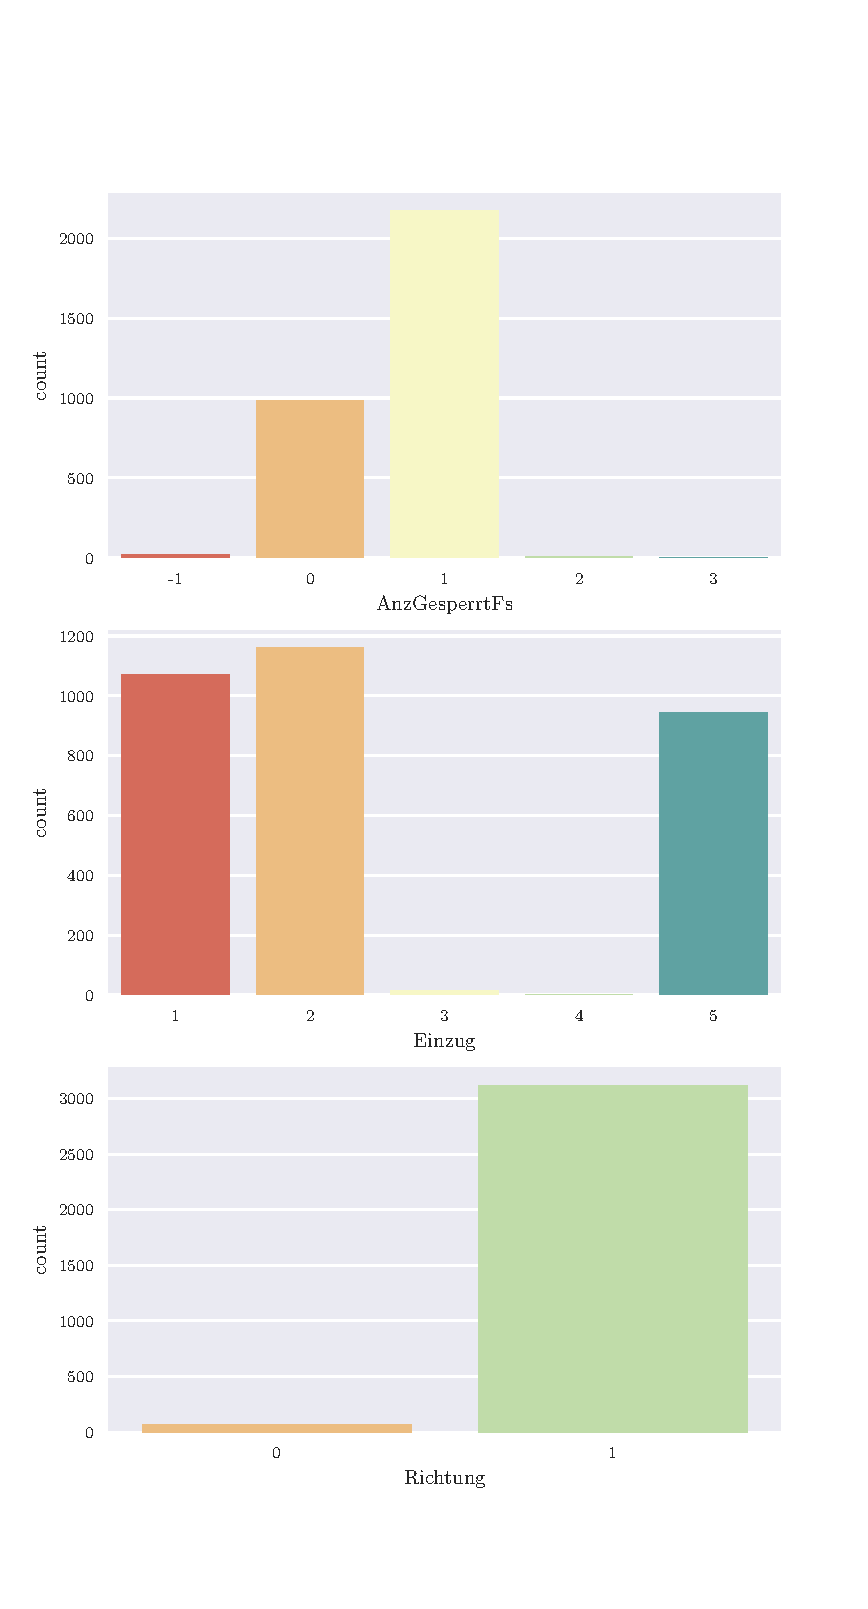
\includegraphics[scale=0.7]{CorrAnalysis/data/ArbIS/02_matched/plots/arbis_matched_count_multiple01}
        \caption{Distribution of the roadwork parameters \textit{AnzGesperrtFs}, \textit{Einzug} and \textit{Richtung}}
        \label{img:arbis_matched_AnzGesperrtFs}
        \label{img:arbis_matched_Einzug}
        \label{img:arbis_matched_Richtung}
    \end{figure}

    \begin{figure}[ht!]
        \centering
        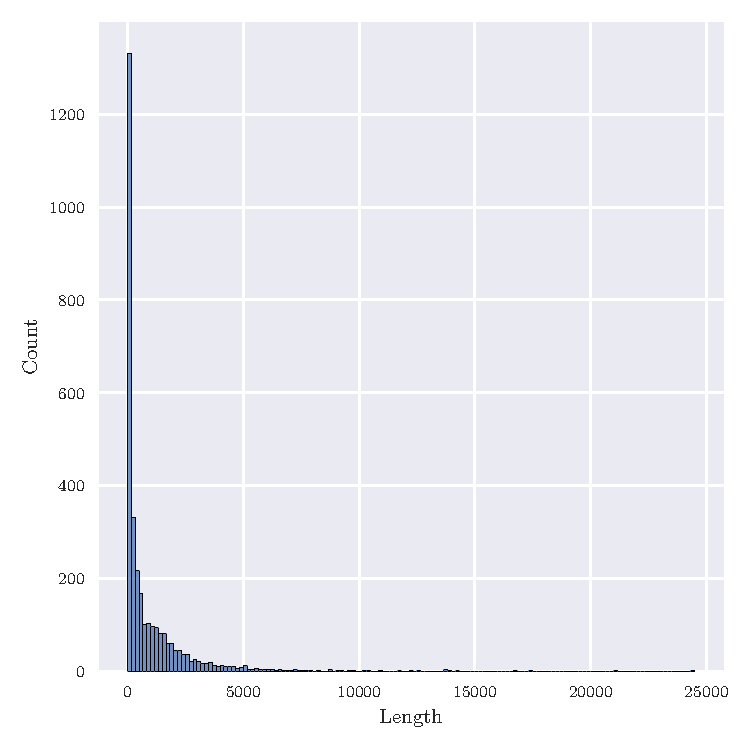
\includegraphics[scale=0.7]{CorrAnalysis/data/ArbIS/02_matched/plots/arbis_matched_dist_Length}
        \caption{Distribution of the roadwork parameter \textit{Length}}
        \label{img:arbis_matched_Length}
    \end{figure}

    \begin{figure}[ht!]
        \centering
        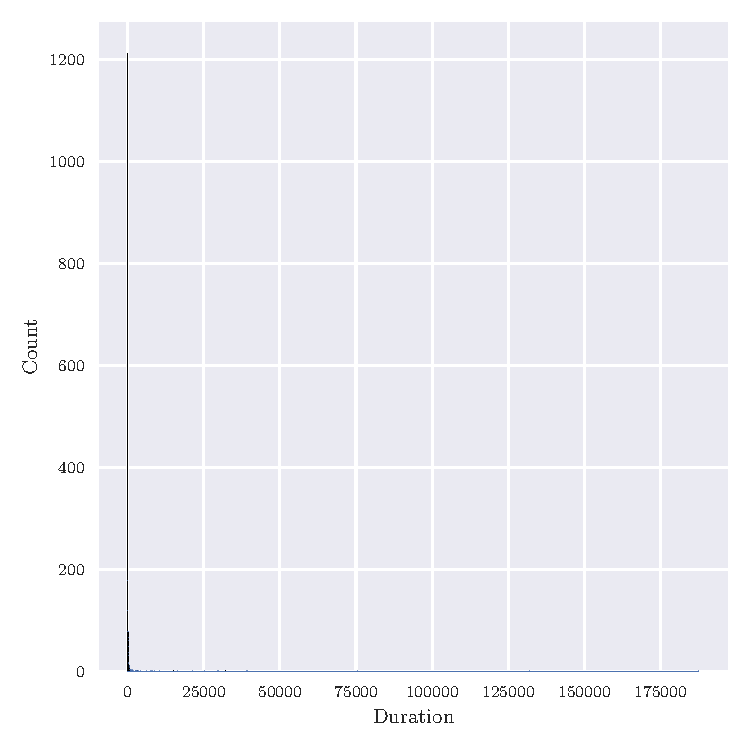
\includegraphics[scale=0.7]{CorrAnalysis/data/ArbIS/02_matched/plots/arbis_matched_dist_Duration}
        \caption{Distribution of the roadwork parameter \textit{Duration}}
        \label{img:arbis_matched_Duration}
    \end{figure}

    % ------- ArbIS Matched - Tables --------
    % \newgeometry{left=1cm,right=1cm,top=1cm}
    \begin{sidewaystable}
        \tiny
        \setlength{\tabcolsep}{4pt}
        \centering
        \begin{tabular}{lrrrrrrrrrrrrrrrr}
\toprule
{} &  TMax &  TAvg &  SMax &  SAvg &  TDist &  SDist &   Cov &  TLCar &  TLHGV &   Str &  AnzGesperrtFs &  Einzug &  Richtung &  Length &  Duration &  Month \\
\midrule
TMax          &  1.00 &  0.80 &  0.54 &  0.47 &  -0.18 &  -0.02 & -0.18 &   0.06 &   0.00 &  0.01 &          -0.04 &    0.02 &      0.02 &    0.06 &      0.02 &   0.13 \\
TAvg          &  0.80 &  1.00 &  0.24 &  0.43 &  -0.17 &  -0.00 &  0.20 &   0.04 &   0.03 & -0.01 &           0.06 &   -0.07 &      0.02 &   -0.00 &      0.02 &   0.20 \\
SMax          &  0.54 &  0.24 &  1.00 &  0.72 &  -0.14 &  -0.08 & -0.48 &   0.00 &  -0.04 & -0.04 &          -0.13 &    0.12 &     -0.01 &    0.13 &      0.00 &   0.20 \\
SAvg          &  0.47 &  0.43 &  0.72 &  1.00 &  -0.16 &  -0.11 &  0.01 &   0.00 &  -0.00 & -0.09 &          -0.06 &    0.04 &     -0.02 &    0.07 &      0.00 &   0.14 \\
TDist         & -0.18 & -0.17 & -0.14 & -0.16 &   1.00 &   0.07 & -0.02 &   0.00 &   0.02 & -0.09 &          -0.04 &    0.00 &      0.01 &   -0.06 &     -0.02 &   0.15 \\
SDist         & -0.02 & -0.00 & -0.08 & -0.11 &   0.07 &   1.00 & -0.07 &   0.01 &   0.01 & -0.03 &          -0.06 &    0.09 &      0.03 &   -0.11 &     -0.01 &   0.13 \\
Cov           & -0.18 &  0.20 & -0.48 &  0.01 &  -0.02 &  -0.07 &  1.00 &  -0.07 &  -0.03 &  0.08 &           0.17 &   -0.16 &     -0.00 &   -0.11 &     -0.01 &   0.22 \\
TLCar         &  0.06 &  0.04 &  0.00 &  0.00 &   0.00 &   0.01 & -0.07 &   1.00 &   0.10 & -0.07 &          -0.03 &    0.01 &     -0.02 &    0.02 &      0.00 &   0.14 \\
TLHGV         &  0.00 &  0.03 & -0.04 & -0.00 &   0.02 &   0.01 & -0.03 &   0.10 &   1.00 & -0.08 &          -0.02 &    0.01 &      0.03 &    0.00 &      0.02 &   0.12 \\
Str           &  0.01 & -0.01 & -0.04 & -0.09 &  -0.09 &  -0.03 &  0.08 &  -0.07 &  -0.08 &  1.00 &          -0.02 &    0.05 &     -0.02 &   -0.04 &     -0.02 &   0.27 \\
AnzGesperrtFs & -0.04 &  0.06 & -0.13 & -0.06 &  -0.04 &  -0.06 &  0.17 &  -0.03 &  -0.02 & -0.02 &           1.00 &    0.50 &      0.18 &   -0.02 &      0.14 &   0.10 \\
Einzug        &  0.02 & -0.07 &  0.12 &  0.04 &   0.00 &   0.09 & -0.16 &   0.01 &   0.01 &  0.05 &           0.50 &    1.00 &      0.14 &    0.03 &     -0.13 &   0.14 \\
Richtung      &  0.02 &  0.02 & -0.01 & -0.02 &   0.01 &   0.03 & -0.00 &  -0.02 &   0.03 & -0.02 &           0.18 &    0.14 &      1.00 &   -0.05 &     -0.07 &   0.14 \\
Length        &  0.06 & -0.00 &  0.13 &  0.07 &  -0.06 &  -0.11 & -0.11 &   0.02 &   0.00 & -0.04 &          -0.02 &    0.03 &     -0.05 &    1.00 &      0.07 &   0.09 \\
Duration      &  0.02 &  0.02 &  0.00 &  0.00 &  -0.02 &  -0.01 & -0.01 &   0.00 &   0.02 & -0.02 &           0.14 &   -0.13 &     -0.07 &    0.07 &      1.00 &   0.05 \\
Month         &  0.13 &  0.20 &  0.20 &  0.14 &   0.15 &   0.13 &  0.22 &   0.14 &   0.12 &  0.27 &           0.10 &    0.14 &      0.14 &    0.09 &      0.05 &   1.00 \\
\bottomrule
\end{tabular}

        \caption{Correlation matrix for ArbIS matched data, calculated with Cramer's $V$, $\eta$, $\tau$, $r_{pq}$, $r$}
    \end{sidewaystable}
    \begin{sidewaystable}
        \tiny
        \setlength{\tabcolsep}{4pt}
        \centering
        \begin{tabular}{lrrrrrrrrrrrrrrrr}
\toprule
{} &  TMax &  TAvg &  SMax &  SAvg &  TDist &  SDist &   Cov &  TLCar &  TLHGV &   Str &  AnzGesperrtFs &  Einzug &  Richtung &  Length &  Duration &  Month \\
\midrule
TMax          &  1.00 &  0.80 &  0.54 &  0.47 &  -0.18 &  -0.02 & -0.18 &   0.06 &   0.00 &  0.01 &          -0.04 &    0.02 &      0.02 &    0.06 &      0.02 &   0.13 \\
TAvg          &  0.80 &  1.00 &  0.24 &  0.43 &  -0.17 &  -0.00 &  0.20 &   0.04 &   0.03 & -0.01 &           0.06 &   -0.07 &      0.02 &   -0.00 &      0.02 &   0.20 \\
SMax          &  0.54 &  0.24 &  1.00 &  0.72 &  -0.14 &  -0.08 & -0.48 &   0.00 &  -0.04 & -0.04 &          -0.13 &    0.12 &     -0.01 &    0.13 &      0.00 &   0.20 \\
SAvg          &  0.47 &  0.43 &  0.72 &  1.00 &  -0.16 &  -0.11 &  0.01 &   0.00 &  -0.00 & -0.09 &          -0.06 &    0.04 &     -0.02 &    0.07 &      0.00 &   0.14 \\
TDist         & -0.18 & -0.17 & -0.14 & -0.16 &   1.00 &   0.07 & -0.02 &   0.00 &   0.02 & -0.09 &          -0.04 &    0.00 &      0.01 &   -0.06 &     -0.02 &   0.15 \\
SDist         & -0.02 & -0.00 & -0.08 & -0.11 &   0.07 &   1.00 & -0.07 &   0.01 &   0.01 & -0.03 &          -0.06 &    0.09 &      0.03 &   -0.11 &     -0.01 &   0.13 \\
Cov           & -0.18 &  0.20 & -0.48 &  0.01 &  -0.02 &  -0.07 &  1.00 &  -0.07 &  -0.03 &  0.08 &           0.17 &   -0.16 &     -0.00 &   -0.11 &     -0.01 &   0.22 \\
TLCar         &  0.06 &  0.04 &  0.00 &  0.00 &   0.00 &   0.01 & -0.07 &   1.00 &   0.10 & -0.07 &          -0.03 &    0.01 &     -0.02 &    0.02 &      0.00 &   0.14 \\
TLHGV         &  0.00 &  0.03 & -0.04 & -0.00 &   0.02 &   0.01 & -0.03 &   0.10 &   1.00 & -0.08 &          -0.02 &    0.01 &      0.03 &    0.00 &      0.02 &   0.12 \\
Str           &  0.01 & -0.01 & -0.04 & -0.09 &  -0.09 &  -0.03 &  0.08 &  -0.07 &  -0.08 &  1.00 &          -0.02 &    0.05 &     -0.02 &   -0.04 &     -0.02 &   0.27 \\
AnzGesperrtFs & -0.04 &  0.06 & -0.13 & -0.06 &  -0.04 &  -0.06 &  0.17 &  -0.03 &  -0.02 & -0.02 &           1.00 &    0.83 &      0.01 &   -0.02 &      0.14 &   0.03 \\
Einzug        &  0.02 & -0.07 &  0.12 &  0.04 &   0.00 &   0.09 & -0.16 &   0.01 &   0.01 &  0.05 &           0.50 &    1.00 &      0.00 &    0.03 &     -0.13 &   0.03 \\
Richtung      &  0.02 &  0.02 & -0.01 & -0.02 &   0.01 &   0.03 & -0.00 &  -0.02 &   0.03 & -0.02 &           0.05 &    0.03 &      1.00 &   -0.05 &     -0.07 &   0.06 \\
Length        &  0.06 & -0.00 &  0.13 &  0.07 &  -0.06 &  -0.11 & -0.11 &   0.02 &   0.00 & -0.04 &          -0.02 &    0.03 &     -0.05 &    1.00 &      0.07 &   0.09 \\
Duration      &  0.02 &  0.02 &  0.00 &  0.00 &  -0.02 &  -0.01 & -0.01 &   0.00 &   0.02 & -0.02 &           0.14 &   -0.13 &     -0.07 &    0.07 &      1.00 &   0.05 \\
Month         &  0.13 &  0.20 &  0.20 &  0.14 &   0.15 &   0.13 &  0.22 &   0.14 &   0.12 &  0.27 &           0.01 &    0.02 &      0.00 &    0.09 &      0.05 &   1.00 \\
\bottomrule
\end{tabular}

        \caption{Correlation matrix for ArbIS matched data, calculated with Theil's $U$, $\eta$, $\tau$, $r_{pq}$, $r$}
    \end{sidewaystable}
    \begin{sidewaystable}
        \tiny
        \setlength{\tabcolsep}{4pt}
        \centering
        \begin{tabular}{lrrrrrrrrrrrrrrrr}
\toprule
{} &  TMax &  TAvg &  SMax &  SAvg &  TDist &  SDist &   Cov &  TLCar &  TLHGV &   Str &   AGF &  Einzug &  Richtung &  Length &  Duration &  Month \\
\midrule
TMax     &   nan & 0.000 & 0.000 & 0.000 &  0.000 &  0.385 & 0.000 &  0.001 &  0.965 & 0.000 & 0.024 &   0.107 &     0.267 &   0.001 &     0.173 &  0.000 \\
TAvg     & 0.000 &   nan & 0.000 & 0.000 &  0.000 &  0.953 & 0.000 &  0.047 &  0.071 & 0.000 & 0.011 &   0.000 &     0.301 &   0.987 &     0.340 &  0.000 \\
SMax     & 0.000 & 0.000 &   nan & 0.000 &  0.000 &  0.000 & 0.000 &  0.859 &  0.034 & 0.000 & 0.000 &   0.000 &     0.451 &   0.000 &     0.993 &  0.000 \\
SAvg     & 0.000 & 0.000 & 0.000 &   nan &  0.000 &  0.000 & 0.663 &  0.988 &  0.896 & 0.000 & 0.041 &   0.004 &     0.397 &   0.000 &     0.934 &  0.000 \\
TDist    & 0.000 & 0.000 & 0.000 & 0.000 &    nan &  0.000 & 0.201 &  0.819 &  0.190 & 0.000 & 0.452 &   0.765 &     0.506 &   0.001 &     0.163 &  0.000 \\
SDist    & 0.385 & 0.953 & 0.000 & 0.000 &  0.000 &    nan & 0.000 &  0.527 &  0.445 & 0.000 & 0.000 &   0.000 &     0.063 &   0.000 &     0.433 &  0.000 \\
Cov      & 0.000 & 0.000 & 0.000 & 0.663 &  0.201 &  0.000 &   nan &  0.000 &  0.050 & 0.000 & 0.000 &   0.000 &     0.799 &   0.000 &     0.508 &  0.000 \\
TLCar    & 0.001 & 0.047 & 0.859 & 0.988 &  0.819 &  0.527 & 0.000 &    nan &  0.000 & 0.000 & 0.032 &   0.350 &     0.229 &   0.183 &     0.913 &  0.000 \\
TLHGV    & 0.965 & 0.071 & 0.034 & 0.896 &  0.190 &  0.445 & 0.050 &  0.000 &    nan & 0.000 & 0.237 &   0.677 &     0.112 &   0.802 &     0.279 &  0.000 \\
Str      & 0.000 & 0.000 & 0.000 & 0.000 &  0.000 &  0.000 & 0.000 &  0.000 &  0.000 &   nan & 0.000 &   0.000 &     0.000 &   0.000 &     0.000 &  0.000 \\
AGF      & 0.024 & 0.011 & 0.000 & 0.041 &  0.452 &  0.000 & 0.000 &  0.032 &  0.237 & 0.000 &   nan &   0.000 &     0.000 &   0.002 &     0.000 &  0.000 \\
Einzug   & 0.107 & 0.000 & 0.000 & 0.004 &  0.765 &  0.000 & 0.000 &  0.350 &  0.677 & 0.000 & 0.000 &     nan &     0.000 &   0.046 &     0.000 &  0.000 \\
Richtung & 0.267 & 0.301 & 0.451 & 0.397 &  0.506 &  0.063 & 0.799 &  0.229 &  0.112 & 0.000 & 0.000 &   0.000 &       nan &   0.008 &     0.000 &  0.000 \\
Length   & 0.001 & 0.987 & 0.000 & 0.000 &  0.001 &  0.000 & 0.000 &  0.183 &  0.802 & 0.000 & 0.002 &   0.046 &     0.008 &     nan &     0.000 &  0.000 \\
Duration & 0.173 & 0.340 & 0.993 & 0.934 &  0.163 &  0.433 & 0.508 &  0.913 &  0.279 & 0.000 & 0.000 &   0.000 &     0.000 &   0.000 &       nan &  0.000 \\
Month    & 0.000 & 0.000 & 0.000 & 0.000 &  0.000 &  0.000 & 0.000 &  0.000 &  0.000 & 0.000 & 0.000 &   0.000 &     0.000 &   0.000 &     0.000 &    nan \\
\bottomrule
\end{tabular}

        \caption{Significancy matrix for ArbIS matched data}
    \end{sidewaystable}
    \begin{sidewaystable}
        \tiny
        \setlength{\tabcolsep}{4pt}
        \centering
        \begin{tabular}{lllllllllllllllll}
\toprule
{} &      TMax &      TAvg &      SMax &      SAvg &     TDist &     SDist &       Cov &     TLCar &     TLHGV &       Str & AnzGesperrtFs &  Einzug &  Richtung &    Length &  Duration &   Month \\
\midrule
TMax          &       NaN &       $r$ &       $r$ &       $r$ &       $r$ &       $r$ &       $r$ &       $r$ &       $r$ &       $r$ &        $\tau$ &  $\tau$ &  $r_{pq}$ &       $r$ &       $r$ &  $\eta$ \\
TAvg          &       $r$ &       NaN &       $r$ &       $r$ &       $r$ &       $r$ &       $r$ &       $r$ &       $r$ &       $r$ &        $\tau$ &  $\tau$ &  $r_{pq}$ &       $r$ &       $r$ &  $\eta$ \\
SMax          &       $r$ &       $r$ &       NaN &       $r$ &       $r$ &       $r$ &       $r$ &       $r$ &       $r$ &       $r$ &        $\tau$ &  $\tau$ &  $r_{pq}$ &       $r$ &       $r$ &  $\eta$ \\
SAvg          &       $r$ &       $r$ &       $r$ &       NaN &       $r$ &       $r$ &       $r$ &       $r$ &       $r$ &       $r$ &        $\tau$ &  $\tau$ &  $r_{pq}$ &       $r$ &       $r$ &  $\eta$ \\
TDist         &       $r$ &       $r$ &       $r$ &       $r$ &       NaN &       $r$ &       $r$ &       $r$ &       $r$ &       $r$ &        $\tau$ &  $\tau$ &  $r_{pq}$ &       $r$ &       $r$ &  $\eta$ \\
SDist         &       $r$ &       $r$ &       $r$ &       $r$ &       $r$ &       NaN &       $r$ &       $r$ &       $r$ &       $r$ &        $\tau$ &  $\tau$ &  $r_{pq}$ &       $r$ &       $r$ &  $\eta$ \\
Cov           &       $r$ &       $r$ &       $r$ &       $r$ &       $r$ &       $r$ &       NaN &       $r$ &       $r$ &       $r$ &        $\tau$ &  $\tau$ &  $r_{pq}$ &       $r$ &       $r$ &  $\eta$ \\
TLCar         &       $r$ &       $r$ &       $r$ &       $r$ &       $r$ &       $r$ &       $r$ &       NaN &       $r$ &       $r$ &        $\tau$ &  $\tau$ &  $r_{pq}$ &       $r$ &       $r$ &  $\eta$ \\
TLHGV         &       $r$ &       $r$ &       $r$ &       $r$ &       $r$ &       $r$ &       $r$ &       $r$ &       NaN &       $r$ &        $\tau$ &  $\tau$ &  $r_{pq}$ &       $r$ &       $r$ &  $\eta$ \\
Str           &       $r$ &       $r$ &       $r$ &       $r$ &       $r$ &       $r$ &       $r$ &       $r$ &       $r$ &       NaN &        $\tau$ &  $\tau$ &  $r_{pq}$ &       $r$ &       $r$ &  $\eta$ \\
AnzGesperrtFs &    $\tau$ &    $\tau$ &    $\tau$ &    $\tau$ &    $\tau$ &    $\tau$ &    $\tau$ &    $\tau$ &    $\tau$ &    $\tau$ &           NaN &     $V$ &       $V$ &    $\tau$ &    $\tau$ &     $V$ \\
Einzug        &    $\tau$ &    $\tau$ &    $\tau$ &    $\tau$ &    $\tau$ &    $\tau$ &    $\tau$ &    $\tau$ &    $\tau$ &    $\tau$ &           $V$ &     NaN &       $V$ &    $\tau$ &    $\tau$ &     $V$ \\
Richtung      &  $r_{pq}$ &  $r_{pq}$ &  $r_{pq}$ &  $r_{pq}$ &  $r_{pq}$ &  $r_{pq}$ &  $r_{pq}$ &  $r_{pq}$ &  $r_{pq}$ &  $r_{pq}$ &           $V$ &     $V$ &       NaN &  $r_{pq}$ &  $r_{pq}$ &     $V$ \\
Length        &       $r$ &       $r$ &       $r$ &       $r$ &       $r$ &       $r$ &       $r$ &       $r$ &       $r$ &       $r$ &        $\tau$ &  $\tau$ &  $r_{pq}$ &       NaN &       $r$ &  $\eta$ \\
Duration      &       $r$ &       $r$ &       $r$ &       $r$ &       $r$ &       $r$ &       $r$ &       $r$ &       $r$ &       $r$ &        $\tau$ &  $\tau$ &  $r_{pq}$ &       $r$ &       NaN &  $\eta$ \\
Month         &    $\eta$ &    $\eta$ &    $\eta$ &    $\eta$ &    $\eta$ &    $\eta$ &    $\eta$ &    $\eta$ &    $\eta$ &    $\eta$ &           $V$ &     $V$ &       $V$ &    $\eta$ &    $\eta$ &     NaN \\
\bottomrule
\end{tabular}

        \caption{Coefficient matrix for ArbIS matched data}
    \end{sidewaystable}
    % \restoregeometry

\end{appendices}
    


\begin{document}

% -------------------
% |    Title-page    |
% -------------------
% \includepdf[pages=-,templatesize={145mm}{210mm},noautoscale=true,offset=-65 50]{myfile.pdf}
%\includepdf[pages={1},offset=25 -40]{chapters/deckblatt.pdf}
\titlehead{
    \parbox{3cm}{\resizebox*{90pt}{!}{
\includegraphics{images/chair_logo.png}}}    
    \centering Technical University of Munich
    \parbox{3cm}{\resizebox*{90pt}{!}{
\includegraphics{images/tum_logo.png}}}
}
\subject{Master's Thesis}
\title{The search for predictability and correlations between traffic-data based congestion- and incident characteristics -- An exploratory data analysis}
\subtitle{Die Suche nach Vorhersagbarkeit und Korrelationen zwischen verkehrsdatenbasierten Stau- und Ereignismerkmalen -- Eine explorative Datenanalyse}
\author{Jakob Erpf \\
\bigskip
\small Mentoring:\\ 
\small M. Eng. Barbara Karl (TUM)\\ 
\small Dr. - Ing. Matthias Spangler (TUM)\\ 
\small Dipl. - Ing. Stefan Gürtler (S\&W)\\
\small Dipl. - Ing. Johannes Grötsch (LBD)
}
\date{\today}
\publishers{Department of Civil, Geo and Environmental Engineering}
\maketitle % Use latex title page

% ------------------
% |    Abstract    |
% ------------------
\cleardoubleoddpage	
\pdfbookmark[section]{Kurzfassung}{abstract} % Abstract as bookmark
\cleardoubleoddpage

\chapter*{Kurzfassung}
\thispagestyle{empty} %hide page numbers
Aktuelle Navigationssysteme verwenden häufig Akkumulationsstrategien, um die Reisezeit ab- zuschätzen, wobei Zeitverzögerungen durch Staus auf der Grundlage der Historie des zugrunde liegenden Straßennetzes berechnet werden. Dieser Ansatz kann durch ungewöhnliche Ereignisse gestört werden, die kurze Zeitblockaden verursachen, oder durch regelmäßig anfallende, langfristige Verringerungen des Verkehrsaufkommens verzerrt werden. Diese Arbeit evaluiert einen neuen Ansatz zur Vorhersage von Stau- und Unfallmerkmalen durch die Korrelation von Staus und Ereignissen, die in zeitlicher und räumlicher Nähe zueinander liegen. Um dies in einer explorativen Datenanalyse zu evaluieren, werden drei reale Datensätze aus dem Jahr 2019 betrachtet, die Verkehrsbewegungs- und Störfalldaten liefern. Nach einem algorithmischen Ansatz zur Detektion von Staus in FCD Daten und der Lokalisierung räumlich und zeitlich benachbarter Vorfälle aus den BAYSIS und ArbIS Datensätzen wird in der Arbeit mit statistischen Methoden evaluiert, ob und wie diese Vorfälle und Staus miteinander korreliert sind. Daher besteht die Methodik aus dem Clustering von FCD, dem Matching benachbarter Vorfälle, der Korrelations- und Vorhersageanalyse.

Die Ergebnisse zeigen, dass es signifikante Korrelationen zwischen Stau- und Störfallmerkmalen gibt, was bedeutet, dass einzelne Unfallmerkmale statistisch zu Staus mit einer bestimmten Länge und Dauer führen. Dieser Zusammenhang zwischen Länge und Dauer eines Staus ist auch bei den Baustellencharakteristika, wie der Baustellenlage (Straße) und des Baustellenausführungsmonat gegeben. Obwohl diese Korrelationen einen ersten Hinweis auf die Vorhersagbarkeit liefern, ergab eine separate Analyse, dass zwischen keinem der Merkmale Vorhersagbarkeit besteht. An dieser Stelle muss auch angemerkt werden, dass viele Beziehungen nach der Klassifizierung der Daten keine ausreichende Stichprobengröße mehr hatten und ein größerer Datensatz notwendig wäre, um mehr aussagekräftigere und zuverlässigere Ergebnisse zu finden.
\cleardoubleoddpage

\chapter*{Abstract}
\thispagestyle{empty} %hide page numbers
Current navigation systems often use accumulation strategies to estimate travel time while considering time delays through congestions based on analyzing the history of the underlying street network. This approach can be disturbed through uncommon events creating short time blockages or be biased through regular accruing, long-term traffic volume reductions. This thesis evaluates a new approach of predicting congestion and accident characteristics through the correlation of congestions and incidents which are placed in temporal and spatial vicinity of each other. To evaluate this in a exploratory data analysis, three real world datasets from the year 2019 will be considered providing traffic movement and incident data. After an algorithmic approach to analyzing a derivative of a floating car dataset for jams and locating spatial and timely adjacent incidents from the BAYSIS and ArbIS, the thesis will evaluate if and how these incidents and jams are correlated with each other with statistical methods. Therefore the methodology consist of the clustering of FCD, adjacent incident matching, correlation and prediction analysis.

The results show that there are significant correlations between congestion and incident characteristics which means that individual accident characteristics statistical lead to jams with a certain length and duration. This length and duration relationship is also present with the roadwork characteristics of the roadwork's location (road) and the month of the roadwork. Although these correlations provide a first indication of predictability, a separate analysis revealed not predictability between any of the characteristics. At this point it also has to be noted that many relations had insufficient sample size after classifying the data and a larger dataset would be necessary to find more significant and reliable results.


\cleardoubleoddpage	
\chapter*{Erklärung zur Master’s Thesis}
\thispagestyle{empty} %hide page numbers

\enquote{Ich versichere hiermit, die vorliegende Arbeit selbständig verfasst und keine anderen Quellen als die angegebenen Quellen und Hilfsmittel benutzt zu haben. Die Arbeit wurde noch nicht anderweitig für Prüfungszwecke vorgelegt.}

\vspace{4cm}

München, 08.12.2020 : \hrulefill \newline
\hspace*{0mm}\phantom{München, 08.12.2020: } B. Sc. Jakob Erpf

% ---------------------------
% |    Table of contents    |
% ---------------------------
\cleardoubleoddpage	
\pdfbookmark[section]{\contentsname}{toc} % toc is part of the bookmarks but not part the toc itself
\newpage\thispagestyle{empty}
{
  \pagestyle{empty}
  \addtocontents{toc}{\protect\thispagestyle{empty}} 
  \tableofcontents
  \clearpage
}

% ------------------
% |    Chapters    |
% ------------------
\setcounter{page}{1}
\chapter{Introduction}
\setcounter{page}{1}
Traffic \glspl{jam} are a common problem to everyone, ever attempting to begin the summer season with a car trip on the first day of summer break. When the number of road users increases or the capacity of the road way decreases due to various reasons, a imbalance between demand and supply is created \parencite{Tang2019}. This impacts passenger traffic as well as transportation of goods through blocked bottlenecks and decreased travel speeds. They lead to unreliable travel times, inefficient usage of resources, and an increase in emissions, like pollutants or noise \parencite{FHA2011}. Another effect is a decrease in road safety, due to high driver tempers or inattentive mind, which can result in higher accident counts \parencite{Sun2016}. This induces enormous social costs due to billions of hours lost in \glspl{jam} and induced mental stress. \parencite{RetallackOstendorf2019,BardtFritsch2014,ADAC2019}

Therefore it is essential to reduce risks of \glspl{jam}, as well as accidents, with an increased understanding of the traffic accident causes, trigger effects of \glspl{jam} and roadwork consequences, to maintain a fluent traffic flow and traffic safety. Tailored \acrfull{tsm} strategies, focused on automatic reactions for significant traffic event, could enable \acrfull{atdm} of high traffic demands in reduced traffic volume areas \parencite{Tang2019}. This would go towards reducing the economic, environmental, and social costs associated with accidents, roadworks or \glspl{jam}. Part of these \acrshort{tsm} strategies implemented in a \acrshort{atdm} system, could be a form of traffic incident prediction systems, with the potential to identify compromising conditions in real-time, allowing according to actions to be taken to avoid consecutive events. \parencite{RetallackOstendorf2019} 

\bigskip

This thesis approaches \gls{jam} and incident prediction by evaluating the statistical relation of \glspl{jam} and incidents to predict the chance of a consecutive event. These consecutive events can be \glspl{jam}, as well as incidents. Depending on the severity of an accident \glspl{jam} can be provoked. On the other hand \glspl{jam} can facilitate accidents due to the change of traffic flow. Another scenario are construction sites and maintenance which can also lead to both \glspl{jam} and accidents, because of the reduction of traffic volume, changes in road guidance, or other modifications to the actual traffic situation. Although the scope of the thesis does not cover the specifics on a complete production system for \gls{jam} and accident detection, prediction and response, it will take the concept of such a system and focus the possibility of predicting such events, which then would make the development of such a system possible. 

A system capable of the described mentioned functionalities would likely consist of the following processing components.

\begin{itemize}
  \item Acquisition of traffic movement and incident data
  \item Congestion and incident detection
  \item Prediction of consecutive events
  \item Traffic management and controlling responses
\end{itemize}

The second component in charge of detecting \glspl{jam} as well as incident, requires input data like speed, volume, occupancy to represent the traffic situation and incident reports to define incident characteristics. The next component would then analyze the resulting dataset to find characteristic features of the jams and incidents, which will be determined in this thesis. In case the analysis of the characteristic shows a possible and imminent event it would trigger the last component to initiate appropriate controlling actions and prepare incident responses. In the following chapters of this introduction section, the reader will be introduced to the concepts and systems used to cover the input and output requirements in this thesis.

\section{Continuous Floating Data}
\label{introduction_continuous_floating_data}
To detect \glspl{jam} continuous data about the speed or movement of the vehicle on the road is necessary. This kind of information can be collected through a variety of different systems to represent a real-time or at least current picture of the traffic situation. 

The current street network of Bavaria heavily depends on stationary sensors to assess the traffic situation. This includes inductive loops, infrared or radar detectors which can provide traffic indicators like volume, speed, time gaps, jams, density and many others. The data collected with just stationary sensors can only describe the traffic trends restricted to their location and coverage which requires complex simulations and modeling to aggregate data for the missing areas where no sufficient coverage can be provided. Adding to this is the fluctuating result set quality which depends on the input data and simulation model quality. Especially highways are equipped with stationary sensors but the lower index streets network is only covered by a fragmented net of detectors with distances of up to 100\,km between detectors \parencite{INDRIX2015}. Fortunately, nowadays cars as well as drivers and riders are equipped with technology that allows real time tracking and comprehensive data collection. Automobiles can gather information from the build in sensors as well as the on-board GPS. Even mobile devices from drivers and riders can be used to collect location and movement data. \parencite{Randelhoff2016}

\acrfull{fcd} is continuously collected during the usage of a car by the on-board GPS and represents the individual movements. Typically this incorporates the coordinates, timestamp, road section, course and routing data points. These are regularly sent to a central FCD unit/service via mobile radio communication (\acrshort{gsm}-, \acrshort{umts}- or \acrshort{lte}-based) to be aggregated and combined with stationary data to an area wide picture of the traffic situation. In this form they can be used for traffic analysis and management. \parencite{Randelhoff2016,LAPID2020}

A derivative of \acrshort{fcd} is \acrfull{xfcd} developed by BMW. It expands the collection of data points of an \acrshort{fcd} with data from the vehicle sensors and systems like breaks, rain sensors, driver assistance systems and more. These data points add a number of analytic opportunities to generate a more precise and detailed traffic picture. \parencite{LAPID2020}

In contrast to \acrshort{fcd}, \acrlong{fpd} does not need an on-board GPS or car systems to create movement data but assumes that driver’s and rider’s mobile devices will register and deregister at the radio tower along the road. \acrshort{fpd} uses this registration information to determine the radio cell the phone is currently in, how long is stayed in that cell and tracks the devices when switching to another cell or tower. It is therefore able to collect a much larger quantity of datasets but lacks in the accuracy of \acrshort{fcd} which transmit the GPS location of the car itself. That been said, on roads with a high coverage of radio tower like in urban areas or on highways, \acrshort{fpd} is able to achieve a comparable accuracy. Mobile service providers collect this anonymized \acrshort{fpd} and forward them to a traffic management unit, which can analyze the date for disturbances and give feedback through the traffic information channels. \parencite{Randelhoff2016,LAPID2020}

Another type of floating data type is \acrfull{fco}. \acrshort{fco} does not only collect it's own \acrshort{fcd} but also data about it's surroundings with the built-in sensors. This includes the automatic recognition of cross- or opposite traffic, traffic volume or relative speeds to other cars. This additional data not only add detail but also allow for correctional fusion algorithms to reduce uncertainties or errors in the pure \acrshort{fcd}. \parencite{Randelhoff2016}

\section{Street Information Systems}
\label{introduction_street_information_systems}

Besides of having a real-time or current picture of the traffic situation, the concept of the thesis also relies on information about current disturbances or possible triggers of disturbances. 

\subsubsection{\acrfull{baysis}}
For disturbances in form of accidents the \acrfull{baysis}, a publicly available information system from the Bavarian street administration, will be used. The systems task is the acquisition, collection and analysis of street network related information, which contains infrastructure inventory and condition, traffic volumes and other key values, as well as an accident register with detailed reports. An export of this accident register with detailed reports is provided by the \acrfull{zvm} for this thesis.

\subsubsection{\acrfull{arbis}}
Another type of disturbance to consider is roadworks, for which an export from the \acrfull{arbis}, a software tool and database used by the Bavarian infrastructure ministry, will be consulted. The system is used to collect and archive all current, planned and passed roadwork and maintenance projects on the Bavarian state street net-work. With the collected information from \acrshort{arbis}, an effective, economic and safe execution of roadworks can be achieved. Furthermore \acrshort{arbis} can provide detailed report exports about current projects to the Bavarian traffic information office and traffic information channels. \parencite{trafficon2017}

\section{Traffic Status Information}
\label{introduction_traffic_status_information}
To deliver information from traffic management systems to the road users traffic messaging channels can be used. Three known examples are \acrfull{rtti}, \acrfull{tmc} and \acrfull{atis}.

The \acrshort{tmc} is a messenger system for jams and other traffic incidents. The public available service is free to use and publishes current congestion notifications in compatible navigation system and announcements in the local radio channels. In the scope of the \acrshort{tmc} the road network is split into \acrshort{tmc} sections. These sections are used to define the spatial location of the incident to report and typical start or end with road linkups. More detailed Incident information is obtained from the police or reports from traffic participants which adds a considerable before publication delay. It is therefore spatial and temporal to rather imprecise. \parencite{LAPID2020}

Another traffic information source is the \acrshort{rtti}. \acrshort{rtti} supplies traffic participants with information about current events or suggested diversions like \acrfull{tmc}, but with a much spatial higher accuracy. Through a \textit{Geocast}, which is an expansion of a multicast with a geolocation, the spatial precision of the \acrshort{rtti} is superior to the \acrshort{tmc}. This \textit{Geocast} can be either a geometrical address like a GSM84 coordinate or a symbolic address, reaching a spatial accuracy of up to 100m.  \parencite{LAPID2020,HindenDeering2006,ImielinskiNavas1996}. This is why \acrshort{rtti} is the industry standard of suppling vehicle and third party navigation system with up to date traffic information. Another difference to \acrshort{tmc} is the accessibility. Unlike the publicly available \acrshort{tmc}, \acrshort{rtti} is vendor specific and most of the time a payed service, like BMWs ConnectedDrive \parencite{BMW2020}. 

% TODO more infos and literature to TMC / Geocast
% https://ec.europa.eu/transport/themes/its/road/action_plan/traffic-information_en
% https://www.itwissen.info/RTTI-realtime-traffic-information.html
% https://ieeexplore.ieee.org/document/861224

The most up-to-date variation of a traffic status information system is the \acrfull{atis}, such as GoogleMaps, HERE or Waze. Like \acrshort{rtti} it is a provider-based service, but mostly without costs and less device constraint. Because of these missing accessibility constraints and the fact that in current times nearly 70\% of people carry a smartphone \parencite{IZM2020}, the user base of such services is quite substantial. This does not invalidate the usage of \acrshort{rtti} and \acrshort{tmc}, since they are present in most separate and built-in navigational systems, but rather makes \acrshort{atis} a considerable alternative. With the added benefit of being able to not only publish information about the traffic situation but also collect variations of \acrshort{fcd}, \acrshort{atis} is the most promising technology for \acrshort{atdm} and \acrshort{fcd} collection. 

\bigskip

In the scope of this thesis only the following  selection of these introduced data collection systems will be further relevant. 
\begin{itemize}
  \item \acrshort{fcd} for the congestion data
  \item \acrshort{baysis} and \acrshort{arbis} for incident data
  \item \acrshort{atis} for the concept of \acrshort{atdm}
\end{itemize}

%\textcite{} 
%\footcite{}
%\footnote{}.
% \begin{figure}[ht]
%     \includegraphics[width=\textwidth, height=\textheight,keepaspectratio]{}
%     \caption[]{} 
%     \label{fig:}
% \end{figure}

\chapter{Objects of Research}
	This chapter defines the objects or events which will be researched in this thesis. This includes a literature review and descriptive definition of a congestion. For the use in the data analysis jam events with be further defined based on FCD.  

\section{Incident}
		Incidents in the scope of this thesis, an incident can be accidents, as well as ongoing roadwork or maintenance on the Bavarian street network. These are also the events, which the concept of the thesis tries to predict through the analysis of the correlation of said incidents to jams.
	\subsubsection{Accident}
		An accident is an unexpected and unintentional traffic event, that typically results in damages, injuries and reduction of traffic volumes. These events can be triggered by a number of different reasons, where in this thesis the main focus is on the triggers of slow, congested traffic or roadworks.
	\subsubsection{Roadwork}
		As roadwork classifies all static and moving construction sites, as well as temporary blockages or disturbance due to snow clearing, road maintenance and alike. 
	
\section{Congestion}
\label{definition_congestion}

\paragraph{Naming} As there doesn’t exist a clear plural of the noun congestion the term jams will be used in case of multiple congestion. These two terms are seen as interchangeable for their reference to a single or multiple congestion events.

\subsection{Descriptive Definition}
Jams or a single congestion in layman terms are spatial and timely accumulations of traffic participants, resulting in speeds slower or sometimes much slower than free flow. In severe cases this is also often described as stop-and-go or stopped traffic. They are triggered by a reduction of traffic throughput in volume or an increase of traffic demand. Studies have shown that these triggers are usually caused by four categories of disturbances. \parencite{TRB2003,FHA2011}

\subsubsection{Traffic-Influencing Events}

\begin{itemize}
	\item Incidents : Events that disrupt the normal free flow of traffic, like vehicular crashes, breakdowns or debris. These physical obstacles block lanes or hard shoulders, forcing other road users to execute evasive maneuver and deviate from their normal path. This ultimately changes driving behavior, reduces the quality of traffic flow and traveling speed. Even when incidents are not directly on the roadway they can impact the traffic flow due to emergency responses create blockades or ineffective driving behavior of traffic participants gapping on the incident.
	\item Roadwork : Managed and unmanaged construction sites on the roadway that result in physical changes to the highway environment. This includes a reduction of lanes, lane diversion, elimination of hard shoulders or road closures, which reduce the road capacity and reduce travel speeds.
	\item Weather : Changes in environmental conditions like heavy rain or snow fall can negatively impact driver behavior. The reduction of visibility will usually result in a reduction of traveling speeds and increase of headway. This reduces the overall capacity of the highway. Bright sunlight, smoke or icy road surfaces lead to a similar effect.
\end{itemize}

\subsubsection{Traffic Demand}

\begin{itemize}
	\item Fluctuations in Normal Traffic : Variations in demand in day-to-day traffic volumes can overload systems with fixed capacities. This can result in travel speed reductions without any specifically occurring events.
	\item Special Events : Special cases where events drastically change the demand in their vicinity and overload the system. As with incidents, off-road events can affect driving behavior due to visual distractions and change the traffic-flow. 
\end{itemize}

\subsubsection{Physical Highway Features}

\begin{itemize}
	\item Traffic Control Devices : Poorly time or defective traffic signals as well as ineffectively controlling the traffic flow contribute to the creation of jams and travel time reductions.
	\item Physical Bottlenecks or Capacity : The capacity of a road is mostly dependent on the number of lanes and hard shoulder, as well as the alignment (curves and grades). Physical changes on the road environment like in merging areas, tool booths or road endings reduce the capacity and therefore promote the formation of jams. The road capacity can also be influenced by the driving behavior, which heavily depend on the familiarity of the roadway to the driver. Drivers familiar with routinely congested tend to reduce their headway and therefore increase the capacity \parencite{Charlton2013}.
\end{itemize}

\subsubsection{Driving-behavior}
As above-mentioned, driving behavior can influence the traffic flow as well as capacity and is mostly influenced by environment and the familiarity of the road. Research showed that driving on familiar road has a negative effect on safety aspects of driving behaviors, like in-attentional blindness for roadside features \parencite{Charlton2013}. Another decreasing factor is the state-of-mind, better known as rage- or aggressive driving, resulting in rapid lane changing, cross cutting or passing on shoulders \parencite{Shinar2004}. This can lead to driving behaviors where drivers don't keep up smooth accelerations, but rather break suddenly or accelerate in rapidly, other vehicles need to react accordingly. This creates a chain reaction leading to reduced travel speed. These are called \textit{phantom jams} because they do not have any specific origin and are common in high density traffic regions like cities and high demand highways. \parencite{ASTRA2020} 

\bigskip

This general layman's definition of jams is essential correct, but not sufficient for the data scientific approach in this thesis. The Bavarian ministry for streets does not have an official definition at the time of writing and there is no unified definition or thresholds when reduced speed or time delays can classify data as a congested or slow. This makes it necessary to form a specific definition of \glspl{jam} and their speed/space/time thresholds, for the scope of this thesis. For instance the \acrshort{adac} classifies highway traffic moving with mean speed lower than 20 km/h as jammed \parencite{ADAC2019}. In Switzerland the ministry for streets has a more severe definition with a mean speed of under 10 km/h \parencite{ASTRA2020}. A definition just this available literature does not consider the data is would be applied on. Therefore the representation of the speeds occurring in jams from the FCD dataset, introduced in \cref{dataset_fcd}, should be adducted to further tailor a definition to our needs. 

\subsection{Data Scientific Definition}

\begin{figure}[ht]
	\centering
	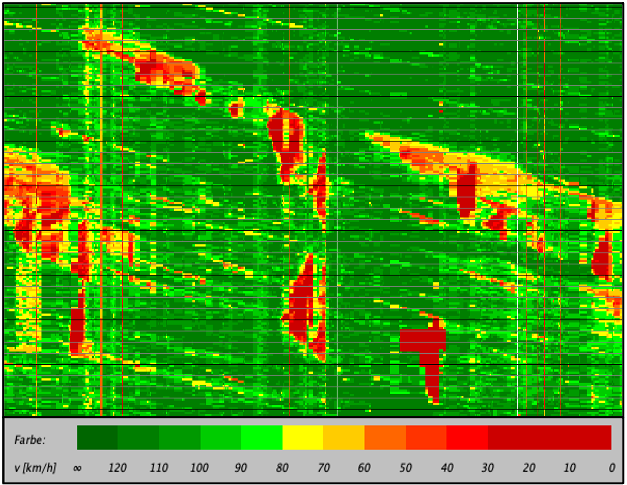
\includegraphics[scale=0.8]{images/SpeedMatrixPlot_single}
	\caption{Speed matrix plots of FCD data, showing a scattered cluster}
	\label{img:speedMatrixPlot_singleCluster}
\end{figure}

\todo{Matrix neu machen, mit bessere Lesbarkeit}

Figure \ref{img:speedMatrixPlot_singleCluster} shows a section of a random speed matrix plot from the \acrshort{fcd} dataset, containing a scattered congestion cluster. The horizontal and vertical extend represents the spatial and temporal location of each cell. The color of the cell indicated the mean absolute speed recorded in the time frame and on the link of the cell (detailed gradient is shown in the legend of \cref{img:speedMatrixPlot_singleCluster}).

The visual representation shows that a congestion mostly contains speed of less than 30 km/h, shown in \textit{dark red}. A closer look on the cluster in the top left reveals that speed around 40-50 km/h, shown in \textit{lighter red} tones, may be also considered, to incorporate the complete congestion area. Speeds above at least 50 km/h, starting with the \textit{orange/yellow} categories, should not be included in the definition, because it would classify regular speed limits, represented by the broad vertical \textit{orange/yellow} stripe, as jammed traffic. This makes two speed threshold for jammed and slow-moving traffic necessary to adequately detecting congestion clusters. With this information and some learning during calibration of the clustering algorithm (see \cref{methodology_detection_clustering}) the following thresholds for the jammed and slow speed, classifying \glspl{jam} in FCD data where defined.

\begin{itemize}
	\item Speed threshold for jammed state : $v_{crit,jammed} = 30\,\frac{km}{h}$
	\item Speed threshold for slow-moving state : $v_{crit,slow} = 60\,\frac{km}{h}$
\end{itemize}

To exclude cell errors and discard detections, too small to have to be considered as jams, the length and duration is used for filtering. 

\begin{itemize}
	\item Minimum length of a congestion : $l_{min} = 1000\,m$
	\item Minimum duration of a congestion : $t_{min} = 9\,min$
\end{itemize}

If $l < l_{min}$ or $t < t_{min}$ is given, $l$ being the maximum spatial extend and $t$ being the maximum temporal extend, the detection should be ignored.

\chapter{Applied Statistic Methods}
\label{definition_correlation}
This chapter will explain the implemented statistical methods and their mathematical definitions. This should result in a deep understanding how the results which are presented in the upcoming chapters are comprised. It also clarifies which methods and assumptions are implemented to handle a mixed data-based analysis.

\bigskip

Correlation is an analysis procedure that measures the correlation coefficient, which represents the degree of linear, bivariant, monotonic or other kind of relation, which could also be described as the degree of association between two variables \parencite{HerzSchlicherSiegener1992}. In most statistics the following common types can be found: Pearson's $r$, Kendall's $\tau$, Spearman  $\rho$ or the Point-Biserial correlation \parencite{Ramzai2020,SPSS2020a,SPSS2020b}. Besides off these, there are many more correlation coefficients which vary in their applicability and interpretability. Depending on which type of data variables are to be analyzed, it is necessary to choose an applicable correlation coefficient. The type of data variable and relation combination are the most restricting features for choosing a suitable correlation coefficient. 

\section{Variable Types}
\label{correlation_variable_types}
Data variables can be grouped into continuous and categorical variables, depending on what kind of observation they describe. Variables are considered to be continuous, also known as quantitative, when relating to measurements like speed, distance or age, which can take on an unlimited number of values between the lowest and highest points of measurement \parencite{McCue2007}. These continuous variables can be separated into two subsets. 

\begin{itemize}
	\item \textbf{Interval} variables can be measured along a continuum and have a numerical value. \parencite{Laerd2020}
    \item \textbf{Ratio} variables are interval variables, with the added condition that the values are zero if there is no measurement for this value. \parencite{Laerd2020}
\end{itemize}

Categorical variables on the other hand are limited in the number of values, referring to a category, rank or choice, like a vehicle type or Yes/No answers. These categorical variables can be separated into three subsets.

\begin{itemize}
	\item \textbf{Nominal} variables have two or more categories, but with no intrinsic order. \parencite{Laerd2020}
	\item \textbf{Dichotomous} are nominal variables which have only two categories or levels. \parencite{Laerd2020}
    \item \textbf{Ordinal} are nominal variables that have two or more categories and are ordered or ranked. \parencite{Laerd2020}
\end{itemize}

The datasets to be examined in this thesis include continuous variables of the type interval and all three types of categorical variables (see \cref{dataset_baysis,dataset_arbis}).

\section{Correlation Types}
\label{correlation_coefficient_types}
The datasets from \acrshort{baysis}, \acrshort{arbis} (see \cref{dataset_baysis,dataset_arbis}) and the processing tool (see \cref{methodology_data_processing}) includes continuous, as well as categorical variables, describing interval, nominal, dichotomous and ordinal characteristics. For an exact analysis of relations between these characteristics the appropriate correlation coefficient suited for the apparent variables needs to be chosen. This task itself is quite complex due to the number of coefficients to evaluate, amount of literature, numerous assumptions and disagreements in the field of statistics. From a comprehensive literature review the following correlation coefficients and tests were selected because of their appearance in current studies and papers and in dependency of their suitability for the apparent relation.

For a flattened introduction into correlation statistic, the article of Jun Ye \textit{Everything you need to know about correlation}\footnote{https://junye0798.com/post/everythin-you-need-to-know-about-correlation/} is highly recommended. \parencite{Yun2020}

\subsection{Continuous - Continuous}
\label{correlation_pearson}

As stated in \cref{correlation_variable_types} continuous variables are metric measurements in form of distances or durations. The most common correlation coefficient for continuous variables is the so called non-parametric Pearson's $r$.

\subsubsection{Pearson's $r$}

Pearson's $r$ describes the linear correlation of such continuous, non-ranked variables and does not assume normality or a normal distributed sample set as it is non-parametric. It is therefore suitable for the examination of continuous - continuous variable relations, where finite size of variance and covariance can be assumed. \parencite{BenestyChenHuang2009,Sulthan2018}
 
The general correlation coefficient, shown in \cref{formula_correlation_basic} is the foundation for deducing Pearson's $r$. It is defined by the fraction of the covariance, \cref{formula_correlation_covariant} of two vectors $x$ / $y$ of length $i$ / $j$ and their standard deviation, see \cref{formula_correlation_deviation}. \parencite{HerzSchlicherSiegener1992}

\smallskip

\begin{equation}
\label{formula_correlation_basic}
	\rho = \frac{\sigma_{xy}}{\sigma_{x}\sigma_{y}}
\end{equation}

\begin{equation}
\label{formula_correlation_covariant}
	\sigma_{xy} = \sum_{ij}(x_i-\mu_X)(y_n-\mu_Y) \cdot p(x_i,y_j)
\end{equation}

\begin{equation}
\label{formula_correlation_deviation}
	\sigma_{x,y} = \sum_{i}(x_i,y_i-\mu_{x,y})^2 \cdot p_i
\end{equation}

\bigskip

The \cref{formula_pearson} shows Pearson's correlation coefficient $r$, which is a direct usage of the definition in \cref{formula_correlation_basic}, assuming that both data variables have the same length, named $i$. The symbols $\bar{x}$ and $\bar{y}$ correspond to the means of the data variable $x$ and $y$, respectively. \parencite{BenestyChenHuang2009,Zychlinski2018}

\smallskip

\begin{equation}
\label{formula_pearson}	
	r_{xy} =  \frac{\sum_{i}{(x_i-\bar{x})(y_i-\bar{y})}}{\sqrt{\sum_{i}{(x_i-\bar{x})^2}\sum_{i}{(y_i-\bar{y})^2}}}
\end{equation}

\bigskip

This equation can be simplified to \cref{formula_pearson_simplified} with the $SS$ corresponding to the summed squares and $SP$ corresponding to summed products.

\smallskip

\begin{equation}
\label{formula_pearson_simplified}
	r =  \frac{SP_{xy}}{\sqrt{SS_x SS_y}}
\end{equation}

\subsubsection{Interpretation of $r$}
Pearson's $r$ can have values of the range $-1$ to $+1$. If one variable moves in the same direction as the other, it is called positive correlation, represented by a positive correlation coefficient. In the case of one variable moving in a positive direction, whereas a second variable is moving in a negative direction, the correlation is called negative and has a negative coefficient. Another characteristic is the ration of change in the variables. When both variables change at the same ratio, they are linearly correlated. When both variables do not change in the same ratio, then they are non-linearly or curvy-linear correlated. 

\subsubsection{Interpretation of effect size $|r|$}
The degree of correlation, also described as strength of association is called effect size and shows how strong two variables are related with each other. It is defined specifically for Person's $r$ as the absolute values of $r$, mathematical written as $|r|$. According to Cohen \parencite{Cohen1988} the effect sizes of each correlation coefficient falls into one of two categories $D$ and $R$. $D$ corresponds to coefficients utilizing the mean difference and standardized mean difference. He defined the values of $D$ coefficients as small $D$ = .20, medium $D$ = .50, and large $D$ = .80 \parencite{Piegorsch2002}. The group of $R$ coefficients includes measures based on variance \parencite{Walker2005}. Cohen proposes vastly different values of .01, .06, and .14 as indicators of small, medium, and large effect sizes for the $R$ group \parencite{Cohen1988}. However, if these values fit the purpose of the analysis, depends on the underlying data and is at discretion of the researcher.

\todo{If .. then ??}

% http://www.leeds.ac.uk/educol/documents/00002182.htm
% https://www.psychometrica.de/effect_size.html
% https://www.cedu.niu.edu/~walker/personal/Walker%20Kendall's%20Tau.pdf

According to Cohen recommendations for mean-based coefficients \parencite{Cohen1988,Piegorsch2002,Walker2005} and with consideration of the guidelines of Wolfe \parencite{Wolfe2017} and Regber \parencite{Regber2016}, which induces an increased scale due to the high sensitivity of Pearson's $r$, the following rules are defined for the interpretation of the effect size of $r$.

\begin{itemize}
  \item When both variables change in the same ratio, the absolute value is 1.0, which is called perfect correlation.
  \item If the range is above .80, it is called high degree of correlation.
  \item A moderate degree of correlation lays in the range of .50 to .80.
  \item When the range is between .30 to .50, it is called low degree of correlation.
  \item If the range is lower than .30 no correlation can be proven. It is called absence of correlation.
\end{itemize}	

There a many other effect sizes like Cohen's $w$, $f^2$ or Heghes $g$, which can be used for the interpretation of relations. But there is also a high amount of contradictions from one source to another, depending on the author, time of publication and data foundation. The interpretation of $r$ and its associated definition by Cohen is the most robust and common ground found in literature and will be used as a mathematical and guideline base for other correlation coefficients.
% https://de.wikipedia.org/wiki/Effektst%C3%A4rke#Umrechnung_in_r

\subsubsection{Significance of $r$}
To determine if $r$ is statically significant a chi-square test is generally applied to find the $p$-value, testing the probability of independence (see \cref{correlation_significance}). 

\subsection{Continuous - Nominal}
This type of relation is objectively the most complex to evaluate. One well known method to analyze the relation between a continuous and categorical variable, which is not ranked and has more than two values, is the analysis of variance (ANOVA). Unfortunately, it assumes normal or gaussian distributed variables, which are not given in the dataset (see \cref{data}), as it is categorized as a parametric test. A non parametric approach of the ANOVA is the rather uncommon Kruskal-Wallis H-test \parencite{Leon1998}. Both tests indicate if at least one variable stochastically dominates another, but not in which groups or in how many groups this domination occurs \parencite{OTSD2020}. They therefore do not provide a statement about the correlation strength, but the statistical significance of variances between groups.

Further research of a non-parametric correlation coefficient only provided one suitable option, eta ($\eta$) coefficient from Pearson \parencite{Benninghaus2007}, describing the relationship between variables based on the sums of squares used in the ANOVA \parencite{Lewis2012,Benninghaus2007}.

\subsubsection{Eta ($\eta$) coefficient}
% https://stackoverflow.com/questions/52083501/how-to-compute-correlation-ratio-or-eta-in-python/52084418
% https://www.frontiersin.org/articles/10.3389/fpsyg.2013.00863/full
The $\eta$ coefficient, also called correlation ratio, is a measurement for the proportion of the variation in $y$, which is associated with a membership of different groups in $x$ \parencite{Laken2013}. Or mathematically $\eta$ is the squared root of the ratio between $SS_x$ and $SS_y$ \parencite{Shaldehi2013,SAGE2014}. When calculated the value of $\eta^2$ represents the percentage of total variance which can be accounted to a group relation.

\smallskip
\begin{equation}
\label{formula_eta}	
	\eta = \sqrt{\frac{SS_x}{SS_y}}
\end{equation}

\subsubsection{Interpretation of $\eta$}
The coefficient $\eta$ can have values in the range from $0$ to $1$ and equals to Person's $r$ according to \parencite{Laken2013}. The effect size, which is categorized in the $R$ group and can therefore be interpreted as follows \parencite{Regber2016,Cohen1988}.
% https://stats.stackexchange.com/questions/166696/how-do-i-convert-eta2-to-pearsons-r
% https://www.researchgate.net/post/Whats_the_reason_for_deriving_Cohens_w_from_Cramers_V_if_the_latter_is_already_a_measure_of_effect_size
\begin{itemize}
	\item $\eta <= .06$ : The correlation strength is weak
	\item $.06 < \eta < .14$ : A moderate strength of correlation
	\item $\eta >= .14$ : There is a strong correlation
\end{itemize}

\subsubsection{Significance of $\eta$}
The significance evaluation for the $\eta$ coefficient is generally performed via the $p$-value of the Kruskal-Wallis $h$-test, since it is a non-parametric test. It is calculated with the chi-squared test ($\chi^2$), defined in \cref{correlation_significance} \parencite{Filipiak2013}. In the case of both a correlated $\eta$ and a significant $h$-test, the exact related groups need to be determined via a post-hoc test (see \cref{correlation_posthoc}).

\subsection{Continuous - Dichotomous}
The Point Biserial correlation is a special form of the Pearson's $r$ correlation coefficient and suited to evaluate the association of continuous-dichotomous relations. 

\subsubsection{Point Biserial}
The Point Biserial notation, shown in \cref{formula_point_biserial}, can be derived from Person's $r$ with the assumption of $y$ only taking dichotomy values of 0 and 1, so that $\bar{y} = p$. The distinction of the cases

\begin{itemize}
	\item $i \cdot p$ referring to $y=1$ an with $1 - p = q$ bigger than $\bar{y}$
	\item $i \cdot q$ referring to $y=0$ an with $1 - p = -p$ smaller than $\bar{y}$
\end{itemize}
allow to form \cref{formula_point_biserial_from_pearson} from \cref{formula_pearson}, which can be simplified to \cref{formula_point_biserial}. \parencite{Tate1954,CohenWest2003,Bortz2004,DeJesus2019}

\smallskip

\begin{equation}
\label{formula_point_biserial_from_pearson}
	r_{pq} =  \frac{n \cdot p (\bar{x}_{y=1}-\bar{x}) \cdot q + n \cdot p (\bar{x}_{y=0}-\bar{x}) \cdot (-q)}{\sqrt{\sum_{i}{(x_i-\bar{x})^2} \cdot (n \cdot p \cdot q^2 + n \cdot q \cdot (-p)^2)}}
\end{equation}
%\begin{equation}
%\label{formula_point_biserial_from_pearson_simplyfied}
%	r_{pqi} =  \frac{n \cdot p \cdot q \cdot (\bar{x}_{y=1}-\bar{x}_{y=0})}{\sqrt{\sum_{i}{(x_i-\bar{x})^2} \cdot (n \cdot p \cdot q)}}
%\end{equation}
\begin{equation}
\label{formula_point_biserial}
	r_{pq} =  \frac{\bar{x}_{y=1}-\bar{x}_{y=0}}{\sqrt{\sum_{i}{(x_i-\bar{x})^2}}} \cdot \sqrt{n \cdot p \cdot q \cdot} 
\end{equation}

\smallskip

It must be pointed out that if the dichotomous variable is artificially binarized, i.e. there is likely continuous data underlying it, biserial correlation is more a measurement of similarity instead of association.

\subsubsection{Interpretation of $r_{pq}$}
Due to the mathematical similarity of the Point Biserial to the Pearson's $r$, the general interpretation of Pearson's $r$ in \textit{Interpretation of effect size $|r|$} of \cref{correlation_pearson} can be applied to Point Biserial with some adjustments. The range of the Point Biserial coefficient, from $0$ to $1$ removes the direction of correlation from the interpretation. According to Cohen \parencite{Cohen1988} the following can be used as guidelines for the effect size $r_{pq}$ \parencite{Leblanc2017}.

\begin{itemize}
	\item $r_{pq} < \: .30$ : The correlation strength is weak
	\item $\: .30 =< r_{pq} < \: .50$ : A moderate strength of correlation
	\item $r_{pq} >= \: .50$ : There is a strong correlation
\end{itemize}

\subsubsection{Significance of $r_{pq}$}
The significance evaluation of the Point Biserial coefficient is done via the 2-tailed $p$-value, a doubled chi-square test (see \cref{correlation_significance}).

\subsection{Continuous - Ordinal}
For ordinal variables, also called ranked or rank ordered, the commonly used Spearman's $\rho$ can be applied, but should be replaced by Kendall's $\tau$ because of it superiority over Spearman \parencite{Newson2002}. 

\subsubsection{Kendall's $\tau$}
Kendalls $\tau$ evaluates the order of rank pairs, instead of the squared rank difference, which makes is more robust against outliners. Because it can be assumed that the data has ties implemented, the $\tau$ with ties must be used. The general definition is shown in \cref{formula_kendalls_r_complex}, with $P$ referring to the \textit{proversion} and $I$ to the \textit{inversion}. With the assumption that the continuous measurement $x$ is or can be ordered, the ordinal/ranked variable $y$ will be wrongly ordered. After forming all possible rank pairs between $x$ and $y$, $P$ and $I$ can be deduced and $\tau$ can be calculated. \parencite{Reiter2015,Bossart2017}

\begin{itemize}	
	\item[] \textbf{Proversion} ($+$) is the number if pairs, where $x < y$ 
	\item[] \textbf{Inversion} ($-$) is the number of pairs, where $x > y$ 
	\item[] \textbf{Ties} ($0$) are pairs where $x = y$
\end{itemize}

\begin{equation}
\label{formula_kendalls_r_complex}
	\tau = \frac{P-I}{\sqrt{(\frac{n(n-1)}{2}-T_x) \cdot (\frac{n(n-1)}{2}-T_y)}}
\end{equation}
\begin{equation}
\label{formula_kendalls_r_tx}
	T_x = \sum_{i=1}^n \frac{t_{x_i}(t_{x_i}-1)}{2}
\end{equation}
\begin{equation}
\label{formula_kendalls_r_ty}
	T_y = \sum_{j=1}^m \frac{t_{y_j}(t_{y_j}-1)}{2}
\end{equation}
\smallskip

\begin{itemize}
	\setlength\itemsep{0.1em}	
	\item[] $N$ is the total number of rank pairs 
	\item[] $P | I$ are the pro- and inversion of pairs
	\item[] $T_x | T_y$ are the ties in $x$ and $y$
	\item[] $n | m$ are the number of rank bindings in $x$ and $y$
	\item[] $t_{x_i} | t_{x_i}$ are the length of rank bindings in $x$ and $y$
\end{itemize}

\bigskip

Thought transformation we can simplify the general definition to equation \ref{formula_kendalls_r} \parencite{Reiter2015}.

\begin{equation}
\label{formula_kendalls_r}
	\tau = \frac{P-I}{\sqrt{(P+I+T_x) \cdot (P+I+T_y)}}
\end{equation}

\subsubsection{Interpretation of $\tau$}
% https://www.reddit.com/r/AskStatistics/comments/44ypc4/kendall_taus_effect_size_question/
Strictly speaking, Kendall's $\tau$ is not a measure of effect size, like Pearson's $r$, but tends to be of similar magnitude. Because of this similarity the general interpretation defined in the sub section \textit{Interpretation of effect size $|r|$} in \cref{correlation_pearson} can be applied. To adapt the guidelines to the lesser sensitivity of $\tau$, they are scaled downwards \parencite{Regber2016}.

\begin{itemize}
	\item $\tau < \: .30$ : The correlation strength is weak
	\item $\: .30 =< \tau < \: .50$ : A moderate strength of correlation
	\item $\tau >= \: .50$ : There is a strong correlation
\end{itemize}

\subsubsection{Significance}
The significance evaluation of Kendall's $\tau$ coefficient is carried out via the 2-tailed $p$-value, elaborated in \cref{correlation_significance}.

\subsection{Categorical - Categorical}
The Pearson's $\chi^2$ test from \cref{correlation_pearson} can also be applied to categorical data for independence statistics. Two correlation coefficients using $\chi^2$ are Cramer’s $V$ and Theil’s $U$. Both can be used to analyze categorical - categorical relations, but differ in the type of result they provide \parencite{OutsideTwoStandardDeviations2018}. Cramer’s $V$ is a symmetric measure providing a measure of association strength. Theil’s $U$, the uncertainty coefficient, on the other hand is a conditional measure and represents the predictability of an association \parencite{Akoglu2018,StackExchange2020}. Because the Theil’s $U$ measurement of predictability provides a better interpretability, it is the preferred  result choice for the interpretation and implementation. 

\subsubsection{Cramer’s V}

Cramer’s V, also called Cramer's phi ($\Phi_c$), is a measurement for the relation of two nominal variables. In \cref{formula_cramers_v_biased}, showing the notation of Cramer’s $V$, $k$ and $r$ are the number of columns and rows, respectively. $\varphi$, the phi coefficient, is defined by $\frac{{\chi^2}}{n_{ij}}$. The $\chi^2$ shown in \cref{formula_cramers_v_chi} is derived from \cref{formula_chi_squared_simplified} with the expansion to columns and rows. \parencite{Sheskin1997,Bergsma2013}
\smallskip
\begin{equation}
\label{formula_cramers_v_biased}
	V = \Phi_c =  \sqrt{\frac{{\varphi^2}}{min(k-1,r-1)}} = \sqrt{\frac{\frac{{\chi^2}}{n_{ij}}}{min(k-1,r-1)}}
\end{equation}
\begin{equation}
\label{formula_cramers_v_chi}
	\chi^2 =  \sum_{i,j}{\frac{(n_{ij}-\frac{n_i n_j}{n})^2}{\frac{n_i n_j}{n}}}
\end{equation}

\smallskip

The above notation of $\Phi_c$ can be heavily biased, trending to overestimate the strength of relation. It can be corrected with \cref{formula_cramers_v_corrected}, using the corrected notation \cref{formula_cramers_v_phi_corrected} for $\tilde{\varphi^2}$ and \cref{formula_cramers_v_k_corrected} as well as \cref{formula_cramers_v_k_corrected} for $k,r$. \parencite{Bergsma2013}
\smallskip
\begin{equation}
\label{formula_cramers_v_corrected}
	\tilde{V} = \tilde{\Phi_c} = \sqrt{\frac{\tilde{\varphi^2}}{min(\tilde{i_{max}}-1,\tilde{j_{max}}-1)}}
\end{equation}
\begin{equation}
\label{formula_cramers_v_phi_corrected}
	\tilde{\varphi^2} = max(0,\varphi^2 - \frac{(k-1)(r-1)}{n-1})
\end{equation}
\begin{equation}
\label{formula_cramers_v_k_corrected}
	\tilde{k} = k - \frac{(k-1)^2}{n-1}
\end{equation}
\begin{equation}
\label{formula_cramers_v_r_corrected}
	\tilde{r} = r - \frac{(r-1)^2}{n-1}
\end{equation}

\bigskip

\subsubsection{Theil’s U}
% https://rstudio-pubs-static.s3.amazonaws.com/558925_38b86f0530c9480fad4d029a4e4aea68.html
The uncertainty coefficient, also called entropy coefficient, is a measurement for the association between two nominal variables and in comparison to Cramers V, provides a much better predictability statement. It is based on the concept of comparing the entropies of variables to determine a degree of association \parencite{Hoang2019}. The entropy of a distribution (see \cref{formula_theils_hx}) and the conditional entropy (see \cref{formula_theils_hxy}) are used to calculate the uncertainty coefficient $U(X)$ \parencite{Glen2017,Glen2018}, which tells us: given Y, what can fraction can be predicted for X \parencite{Hoang2019}.

\smallskip
\begin{equation}
\label{formula_theils}
	U(X) = \frac{H(X)-H(X|Y)}{H(X)}
\end{equation}
\begin{equation}
\label{formula_theils_hx}
	H(X) = -\sum_{x} p_{X}(x)log p_X(x)
\end{equation}
\begin{equation}
\label{formula_theils_hxy}
	H(X) = -\sum_{x,y} p_{X,Y}(x,y)log p_{X,Y}(x,y)
\end{equation}

% Definition: Theil’s U symmetrical
%\begin{equation}
%\label{formula_theils_sym}
%	U(X,Y) = \frac{H(X)U(X|Y)-H(Y)U(Y|X)}{H(X)+H()Y} = 2[\frac{H(X)+H(Y)-H(X|Y)}{H(X)+H(Y)}]
%\end{equation}

\subsubsection{Interpretation}
For the interpretation of Cramers $V$ an adaption to Pearson's $r$ is necessary, but at the same time quite controversial. Some studies convert $V$ to the effect size $w$ for an equal measurement to $r$ ($r$ is representable over different studies), whereas $V$ is already a measure of effect size by itself. \parencite{Baguley2016}
% https://www.researchgate.net/post/Whats_the_reason_for_deriving_Cohens_w_from_Cramers_V_if_the_latter_is_already_a_measure_of_effect_size
% https://www.researchgate.net/post/How_can_I_intepret_the_effect_sizes_of_Cramers_V_when_DF_3

\smallskip
\begin{equation}
\label{formula_cohens_w}
	w = V \cdot \sqrt{min(i_{max}-1,j_{max}-1)}
\end{equation}

\medskip

As shown in \cref{formula_cohens_w} \parencite{Baguley2016} the conversion from $V$ to $w$ is similar to the reduction of $\phi$ in $V$ (see \cref{formula_cramers_v_corrected}). This advocates the opinion that the conversion to $w$ is necessary within a single study and an adaption of scale is sufficient \parencite{Baguley2016}. In terms of this thesis an adapted scale of effect size according to Ellis is used to interpret $\eta$ in the range of $0$ to $1$ \parencite{Cohen1988,Ellis2010,Hemmerich2019}.

\begin{itemize}
	\item $V < \: .30$ : The correlation strength is weak
	\item $\: .30 =< V < \: .40$ : A moderate strength of correlation
	\item $V >= \: .40$ : There is a strong correlation
\end{itemize}

The values of Theil's $U$ show the predictability of the association, where the following rules for interpretation apply. \parencite{TheilsInt01,TheilsInt02,TheilsInt03}

\begin{itemize}
	\item $U < \: 1$ : The forecasting is better than guessing.
	\item $U \sim \: 1$ : The forecasting is about as good as guessing.
	\item $U > \: 1$ : The forecasting is worse than guessing.
\end{itemize}

\section{Correlation Matrix}
As a result the following correlation coefficients and statistical tests are used for the mixed analysis of continuous and categorical variables. These will be implemented into a processing script in \cref{methodology_correlation_processing}.

\bigskip

\begin{table}[ht]
	\centering
    \begin{tabular}{c|c|c|c|c}
        \toprule
								& \textbf{Ordinal} 	& \textbf{Dichotomous} 	&  \textbf{Nominal}	& \textbf{Continuous}	\\
		\midrule
		\textbf{Ordinal}		& Cramer’s $V$		& Cramer’s $V$			& Cramer’s $V$		& Kendall's $\tau$		\\
		\midrule
		\textbf{Dichotomous}	& Cramer’s $V$		& Cramer’s $V$			& Cramer’s $V$		& Point Biserial $r$	\\
		\midrule
		\textbf{Nominal}		& Cramer’s $V$		& Cramer’s $V$			& Cramer’s $V$		& Eta $\eta$			\\
		\midrule
		\textbf{Continuous}		& Kendall's $\tau$ 	& Point Biserial $r$	& Eta $\eta$		& Pearson's $r$			\\
		\bottomrule
	\end{tabular}
	\caption{Correlation Coefficients Matrix}
	\label{tab:correlation_coefficient_matrix}
\end{table}

\section{Significance vs. Uncertainty}
\label{correlation_significance_uncertainty}
Pure correlation results are not sufficient to prove a relation between variables, especially when using the correlation evidence for predictive purposes. Depending on the sample data, statistical results can be random or biased and therefore need to be examined for their probability of error. This is commonly evaluated via the well known statistical significance. Even thought statistical significance is \textbf{the} common standard procedure for evaluating the probability of error, it became a subject of debate in recent years if statistical significance is to generally used and potential misleading. It is often advocated to additionally used statistical uncertainty instead of only relying on statistical significance. \parencite{Harris2019}

\subsection{Uncertainty}
\label{correlation_uncertainty}
The uncertainty assessment aims to determine if a variable has suitable statistical characteristics for the intended analysis or in colloquial terms, is \textit{fit for the purpose}. The literature research showed that there are a number of different procedures for the evaluation of uncertainty. \textit{The Evaluation of Measurement Data - Guide to the Expression of Uncertainty in Measurement}\footnote{https://www.bipm.org/utils/common/documents/jcgm/JCGM.pdf} (also referred to as GUM) defines reliable but also complex guidelines and is recommended for an in depth understanding of uncertainty evaluation \parencite{Farrance2012}. The complexity of the GUM procedures (which are beyond of the scope of this thesis) and the apparent data foundation favored the usage of simpler methods like the \textit{population sampling error}. \parencite{ONS2020}

The sampling error is the uncertainty created selecting a subset from a population. This can result in poorly distributed variables, which induces a high probability of random correlations based on a small number of samples. A initial review of the variable distributions in the \acrshort{baysis} and \acrshort{arbis} dataset showed that there are many  sample size that below 10, which is an arguably low count. Research into the minimal sample size showed, that for categorical variables a minimal number of 20 ($k=3$) or 200 ($k=10$) should be asserted \cref{Cicchetti1981}. From these guidelines and the exploratory approach of this thesis, variables with a sample size below 10 are considered to be uncertain and associated correlations should be neglected.

\todo{Fix footnote}
% https://www.bipm.org/utils/common/documents/jcgm/JCGM_100_2008_E.pdf

\subsection{Significance}
\label{correlation_significance}
Because statistical results are usually based on sample sets, it is necessary to test if the results can be applied on the population or are significant. This significance of a relation can be evaluated by the common dependent $t$-test which compares the significance value $p$ to the error probability level $\alpha$. The $p$-value is generally calculated via chi-squared, shown in \cref{formula_chi_squared_simplified} (chi-squared statistic), which was taken from Wikipedia and cited from Karl Pearson \parencite{Pearson1990}.

% \begin{equation}
% \label{formula_chi_squared}	
% 	\chi^2 = \sum_{i=1}^{m}{\frac{(N_i-n_{0i})^2}{n_{0i}}}
% \end{equation}

\begin{equation}
\label{formula_chi_squared_simplified}	
	\chi^2 = \sum_{i=1}^{n}{\frac{(O_i-E_i)^2}{E_i}} == N\sum_{i=1}^{n}{\frac{(O_i/N-p_i)^2}{p_i}}
\end{equation}
\begin{itemize}
	\setlength\itemsep{0.1em}	
	\item[] $N$ is the total number of data samples 
	\item[] $O_i$ is the number of data samples with type $i$
	\item[] $E_i = N p_i$ is the expected number of data samples with type $i$
\end{itemize}

\medskip

The $p$-value can then be comprised by comparing $\chi^2$ to a $\chi^2$-distribution by calculation or by using a conversion table \parencite{Piegorsch2002} with the degree of freedom $df = (n_x - 1) \cdot (n_y - 1)$. The resulting  $p$-value is compared to the $\alpha$-level to either accept ($p > \alpha$) or reject ($p <= \alpha$) the null hypothesis \textit{"The means are equal to the population"}. For a 2-tailed $p$-value, $p$ will be doubled to incorporate both ends of the distribution. Usually a value of $.05$ is chosen for $\alpha$ which there will be a 5\,\% risk of falsely rejecting the null hypothesis. Out of this definition the following two interpretations of the correlation coefficient can be drawn. \parencite{Tenny2020,OTSD2020}

\begin{itemize}
	\item $p <= \alpha$ means that the null hypothesis can be rejected and indicates that there is a significant dependency between the two tested variables. It can be concluded that the increase or decrease of one variable does significantly relate to the increase or decrease of the other.
	\item $p > \alpha$ means that there is \textbf{no} significant dependency between the two variables and no conclusion can be drawn for the correlation.
\end{itemize}

\section{Post Hoc}
\label{correlation_posthoc}
In the case of a relation of a categorical variable the correlation effect size and it's significance do not provide any statement on which categories are related. This needs to be further evaluated with a Post Hoc test. In our case the Post Hoc test is based on two separated tests. First the variables will be tested for significance with a Kruskal-Wallis rank sum test. 

% https://www.sciencedirect.com/topics/nursing-and-health-professions/kruskal-wallis-test
\smallskip
\begin{equation}
\label{formula_kruskal_wallis}	
	h = \frac{12}{n(n+1)}\sum_{h}{\frac{S_h^2}{n_h}}-3(n+1)
\end{equation}

\medskip

For Kruskal-Wallis $h$-test the following rules apply. The higher the value of $h$, the higher is the variance between the unique variables. A high $h$ normally supports an already found correlation, but must be tested for significance with $\chi^2$ defined in \cref{correlation_significance}. If the significance or $p$-value is below the $\alpha$-level of $.05$ the null hypothesis can be rejected. This implies that the correlation or variances between the groups are significant. For the identification of which groups create this significant variance the following Wilcoxon-Mann-Whitney, sometimes also called Wilcoxon $T$-test is applied pairwise.

The Wilcoxon $T$-test is a non-parametric univariate alternative to the dependent $t$-test and is the recommended test to use when the data violates the assumption of a normal distribution. The two variations \textit{Mann-Whitney U statistic} and \text{Wilcoxon W sanked sum statistic} can be considered as equivalent. The Wilcoxon ranked sum test will be used in a pairwise approach to compare all groups with each other. 
\begin{figure}[ht]
	\centering
	\begin{tikzpicture}
		\matrix (m) [matrix of math nodes,row sep=3em,column sep=4em,minimum width=2em]
		{
		p(G_1,G_1) & p(G_n,G_1) \\
		p(G_1,G_n) & p(G_n,G_n) \\};
		\path[-stealth]
		(m-1-1) edge node [left] {$1,...,n$} (m-2-1)
				edge (m-1-2)
				edge [dashed,-] node [below] {$p$} node [above] {$0$} (m-2-2)
		(m-2-1.east|-m-2-2) edge node [below] {$1,...,n$} (m-2-2)
		(m-1-2) edge node [right] {} (m-2-2);
  	\end{tikzpicture}	
  	\caption{2-dimensional Wilcoxon ranked sum test significance matrix}
\end{figure}
From the resulting matrix of $p$-values and the analog interpretation with the $\alpha$-level (see \cref{correlation_significance}) the significant groups can be identified. These identified groups are considered to have a significant difference to the other groups and therefore can predictably point to a measurement characteristic from a category or vice versa.

A non significant difference between does not mean that there is no correlation, but only that the sample set and size can not support significancy. There are also cases, where the $p$-value of the correlation coefficient and the general Kruskal-Wallis rank sum test show significant differences in the variable, but the pairwise Wilcoxon ranked sum test does not show any significant differences between the groups. This unfitting difference between the \textit{global} and \textit{specific} significance appears when variables have differences between the samples, but the differences are not reflected by the groups or the sample size is not sufficient to support the significancy of the differences. These controversial correlations can also be evaluated in a exploratory data analysis, keeping in mind their limited interpretability and predictability.

%\todo{Ergänze Effektstärke für Mann-Whitney-U}
%https://statistikguru.de/spss/mann-whitney-u-test/effektstaerke-berechnen-3.html
\chapter{Data Foundation}
\label{data}
In this chapter the provided datasets from the previously mentioned street information systems and the FCD provider will be elaborated. In the beginning an overview of FCD in general and the available dataset is given. To give an overview about which results can be expected, the incident datasets from BAYSIS and ArbIS are presented with descriptive statistic. The most relevant parameters of the datasets will be elaborated and illustrated. The parameters are also categorized in the variable types defined in \cref{correlation_variable_types}.

\section{Floating-Car-Data (FCD)}
\label{dataset_fcd}
As described in \cref{introduction_continuous_floating_data}, \acrshort{fcd} represents the movement of vehicles and can be used to calculate vehicle speeds and trajectories. The provided dataset contains the aggregated absolute and relative speeds for highways and state streets, calculated from \acrshort{fcd} data. The process of speeds estimation with \acrshort{fcd} data is explained in detail by Felix Rampe in chapter 4 of his thesis \textit{Traffic Speed Estimation and Prediction Using Floating Car Data} \parencite{Rempe2018}, but goes beyond the scope of this thesis. The FCD is then mapped onto the HERE \parencite{HERE2020} network, to be compliant with the geolocation system used in the project. Each of these aggregated speeds now represents the mean speed over a three-minute time interval on the corresponding road section. This arrangement of speeds for each time step and space step can be called speed matrix and is the base data for the congestion detection. Figure \ref{img:speedMatrixPlot_mutipleMixedClusters} shows a visual representation a speed matrixes with the horizontal axes being the spatial extend and the vertical axes the time extend.
% TODO add more info about FCD if there is time 
% https://athene-forschung.unibw.de/doc/127445/127445.pdf
% Traffic Speed Estimation and Prediction Using Floating Car Data.pdf

\begin{figure}[ht]
	\centering
	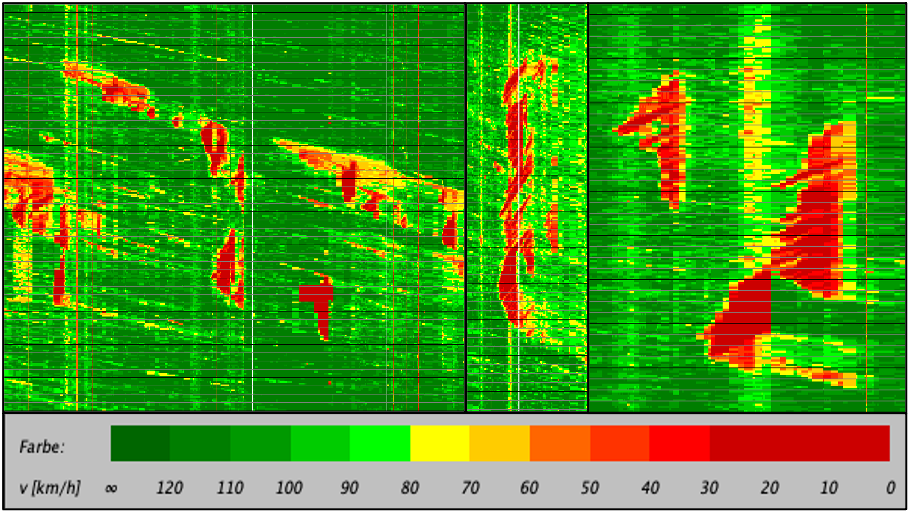
\includegraphics[scale=0.7]{images/SpeedMatrixPlot_mutiple}
	\caption{Speed matrix plots of processed FCD data, showing different jam clusters}
	\label{img:speedMatrixPlot_mutipleMixedClusters}
\end{figure}

Deep greens represent free flowing traffic with 130 km/h, according to the norm speed on highways set the legislator in Germany (in german called “Richtgeschwindigkeit”). The speed scale then develops linearly downwards to deep red indicating traffic with 30 km/h or less. The observer will clearly recognize the jams represented by the clusters of red and orange cells in the \cref{img:speedMatrixPlot_mutipleMixedClusters}. The vehicle trajectory through space and time can be recognize on the angled extends from the top left to the bottom right. From this visual clarity speed matrix and the precision on 3-minute intervals it can be concluded that a comprehensive algorithmic approach should be able to detect such congestion events. This being said, the dataset does contain defects in the form of missing values for complete road sections, which can interfere with detection algorithm. Another defect type would be an obviously wrong speed block, meaning sudden speed drops or jumps to areas of identical speeds with an abnormal temporal and spatial extend, which then have to be ignored during processing. 

\section{Accident Data (BAYSIS)}
\label{dataset_baysis}
The \acrfull{baysis} as described in \cref{introduction_street_information_systems}, collects a wide range of different information types, one of them being accidents with the corresponding police reports. The provided export from BAYSIS contains all accidents of the year 2019 on the Bavarian highway network, which are 10262 records in number. Each accident report includes a variety of specifications which covers environmental indicators like weather or light situation, accident characteristics like accident type, collision object or cause, as well as information over the involved persons like nationality, age and gender. In total, one report contains 132 values describing the accident, participant and environment. As there shouldn't be a stereotype of accident participant formed but rather significant accident characteristics or environmental factors found, most of the descriptive values for the involved persons are not considered. Variables which contain no values or a single values and fall under the uncertainty threshold (see \cref{correlation_uncertainty}) are also neglected. From this curtailed pool of correlate able and analyze able characteristics all parameters that have a logical significance with causes or effects of an accident will be considered in the analysis. The referred figures are available as larger prints in the appendix \cref{appendix_baysis} for better readability, as they do not properly fit in the text. 

\begin{figure}[ht]
	\centering
	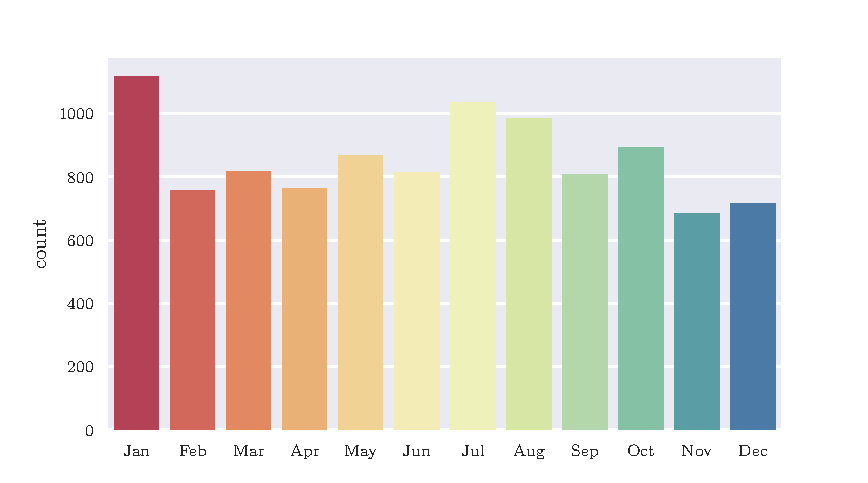
\includegraphics[scale=0.9]{CorrAnalysis/data/BAYSIS/01_dataset/plots/baysis_dataset_hist_month}
	\caption{Distribution of accident counts by months}
	\label{img:baysis_dataset_dist_month}
\end{figure}

A look on the monthly distribution of accidents recorded by BAYSIS (see \cref{img:baysis_dataset_dist_month}) shows that that the months of January, July and August have considerably higher number of accidents, with respectively 31\,\%, 21\,\% and 15\,\% increase over the mean count of 855 accidents per month. The increased number in January can be explained with the increased number of accidents due to ice and snow conditions, which reduces traction on roads and can lead to uncontrollable vehicle behavior. Also the reduced visibility during snow falls increases accident numbers. In July and August the increased traffic volume because of public holidays is the most probable explanation for the higher number of accidents. Another valuable distribution is the number of accidents per road (see \cref{img:baysis_dataset_dist_highway}). The roads A3, A9 and A8 have relative high count of accidents. In contrast the road A71 and downwards have only an accidents and therefore have a high uncertainty associated with them. 

\begin{figure}[ht]
	\centering
	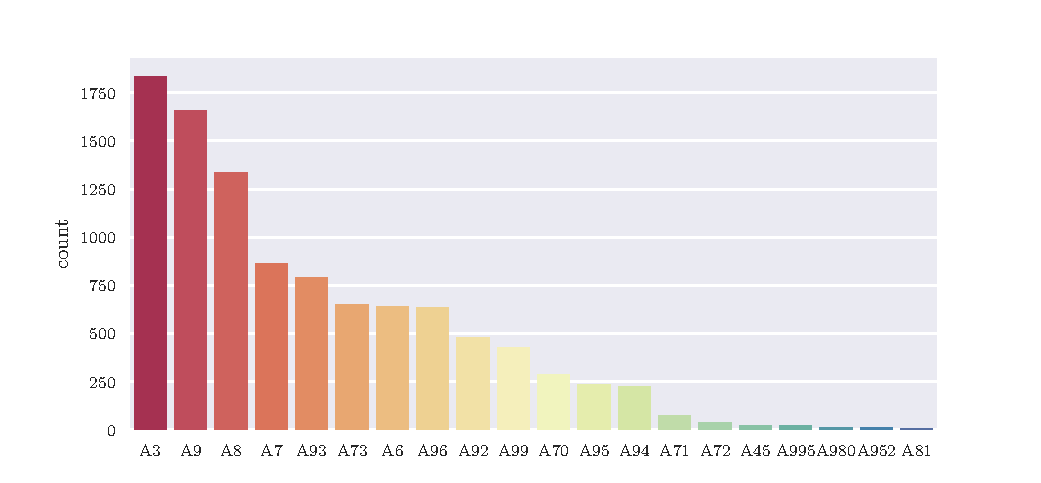
\includegraphics[scale=0.75]{CorrAnalysis/data/BAYSIS/01_dataset/plots/baysis_dataset_hist_highway}
	\caption{Distribution of accident counts by highway}
	\label{img:baysis_dataset_dist_highway}
	\vspace{-8mm}
\end{figure}

\paragraph{Kat}
\label{baysis_dataset_Kat}
The accident category (shown in \cref{tbl:baysis_dataset_Kat} and visualized in \cref{img:baysis_dataset_Kat}), describes the which damages or injuries can be associated with the accident. It ranges from accident with just  damaged property, lightly and heavily injured to deathly accidents. The distribution develops from lowest to highs counts, in order of gravity of the category. The variable consists of four values, which can be ordered, and is therefore ordinal.
\begin{table}[!ht]
	\centering
	\small
	\begin{tabular}{c|c|c|l} 
		\toprule
		Code & Count & Freq. [\%] & Description \\ 
		\midrule
 		0 	& - 	& 	-	& Minor Accident  \\
 		1 	& 76 	& 0.7 	& Accident with deaths  \\ 
 		2 	& 600	& 5.8	& Accident with heavily injured  \\
 		3 	& 2685	& 26.2	& Accident with lightly injured  \\
		7 	& 6900	& 67.2	& Accident with property damage  \\
		\bottomrule
	\end{tabular}
	\caption{Descriptive of \textbf{Kat}}
	\label{tbl:baysis_dataset_Kat}
	% \vspace{-8mm}
\end{table}

\paragraph{Typ}
\label{baysis_dataset_Typ}
The accident type variable (shown \cref{tbl:baysis_dataset_Typ} and visualized in \cref{img:baysis_dataset_Typ}) incorporates different kind of traffic movements, from straight driving to turning movements or merging. It describes during which kind of movement the accident happened. Beside of an 80\,\% share of accidents related to driving or straight driving situations, the parameter does not indicate any other features. The variable does not show any order and is therefore of nominal type.
\begin{table}[!ht]
	\centering
	\small
	\begin{tabular}{c|c|c|l} 
		\toprule
		Code & Count & Freq. [\%] & Description \\ 
		\midrule
 		1 & 2820	& 27.5	& Driving accident \\ 
 		%2 & 1		& < 0.1 & Turning accident \\
 		3 & 373		& 3.6 	& Merging / Crossing accident \\
 		4 & 10		& 0.1	& Crossing over accident \\
 		5 & 160 	& 1.6	& Accident in standing traffic \\
 		6 & 5285	& 51.5	& Accident in straight traffic \\
		7 & 1612	& 15.7 	& Other \\
		\bottomrule
	\end{tabular}
	\caption{Descriptive of \textbf{Typ}}
	\label{tbl:baysis_dataset_Typ}
	\vspace{-8mm}
\end{table}

\paragraph{Betei}
\label{baysis_dataset_Betei}
The distribution of the number of involved persons (shown in \cref{tbl:baysis_dataset_Betei} and visualized in \cref{img:baysis_dataset_Betei}) shows that more than 96\,\% of accidents have three or less involved persons, supported by a mean of 1.9 involved persons. The major share of two involved persons makes up for 56\,\% and the second biggest of one involved person for 30\,\% of the total count. Because of the increasing order of values, the variable is of ordinal type.
\begin{table}[!ht]
	\centering
	\small
	\begin{tabular}{r|ccccccc} 
		\toprule
		 			& 1		& 2		& 3		& 4		& 5		& 6  	& > 7\\ 
		\midrule
 		Count 		& 2768	& 6047	& 1085	& 235	& 72 	& 24	& 30 \\ 
 		Freq. [\%] 	& 27.0	& 58.9	& 10.6 	& 2.3	& 0.7 	& 0.2 	& 0.1 \\
		\bottomrule
	\end{tabular}
	\caption{Descriptive of \textbf{Betei}}
	\label{tbl:baysis_dataset_Betei}
	\vspace{-8mm}
\end{table}

\paragraph{UArt}
\label{baysis_dataset_UArt}
The accident cause type is defined by the two variables \textbf{UArt1} and \textbf{UArt2} (shown in \cref{tbl:baysis_dataset_UArt} and visualized in \cref{img:baysis_dataset_UArt}), whereat the first is the more suitable one. They describe the type of collision cause and presents two major sets. One being the accidents with waiting, stopping and starting vehicles in the same lane, which describe typical collision accidents during congested traffic. The other being the accidents in the next left or right lane, which describe common lane changing collisions. Accidents with cross traffic, pedestrians or opposite traffic are relatively uncommon. The variable does not show any order and is therefore of nominal type.
\begin{table}[ht]
	\centering
	\small
	\begin{tabular}{c|c|c|c|l} 
		\toprule
		Code & Count[1] & Count[2] & Freq. [\%] & Description \\ 
		\midrule
 		1 & 466		& 13	& 4.2  & Collision with starting, standing or stopping vehicle  \\ 
 		2 & 2111	& 44 	& 18.8 & Collision with ahead and waiting vehicle  \\
 		3 & 2873	& 140	& 26.3 & Collision with vehicle on separate lane in same direction  \\
 		4 &	16		& 4		& 0.2   & Collision with vehicle going in opposite direction  \\
 		5 & 240		& 12	& 2.2  & Collision with turning or crossing vehicle  \\
 		6 & 19		& 1		& 0.2   & Collision between vehicle and pedestrian  \\
 		7 & 411		& 42	& 4.0  & Collision with obstacle  \\
 		8 & 1728	& 381	& 18.4 & Deviation to the right  \\
 		9 & 1446	& 517	& 17.1 & Deviation to the left  \\
		0 & 951		& 42	& 8.7  & Other  \\
		\bottomrule
	\end{tabular}
	\caption{Descriptive of \textbf{UArt}}
	\label{tbl:baysis_dataset_UArt}
	%\vspace{-8mm}
\end{table}

\paragraph{AUrs}
\label{baysis_dataset_AUrs}
The summarized distribution of the parameters \textbf{AUrs1} and \textbf{AUrs2} (shown in \cref{tbl:baysis_dataset_AUrs} and visualized in \cref{img:baysis_dataset_AUrs}) shows that the variable is no much distributed and only a small number of categories hold have a relevant sample size. Because of that any correlation to this parameter needs to interpreted with caution, due the the high uncertainty. The variable is of nominal type.
\begin{table}[ht]
	\centering
	\small
	\begin{tabular}{c|c|c|c|l}
		\toprule
		Code & Count[1] & Count[2] & Freq. [\%] & Description \\ 
		\midrule
		%70 & - 	& -		&     & Slippery street due to oil \\
		%71 & -		& -		&     & Slippery street due to dirt \\
		72 & 618	& -		& 33  & Slippery street due to snow or ice \\
		73 & 855	& 45	& 48  & Slippery street due to rain \\
		%74 & -		& -		&     & Slippery street due to other objects \\
		75 & 11		& 12	& 1.2 & Cart track due to rain, snow or ice \\
		76 & 10		& 3		& 0.7 & Other condition of road \\
		%77 & 1		& -		&     & Un-regular condition of traffic signs \\
		%78 & -		& -		&     & Bad lighting of street \\
		%79 & -		& -		&     & Bad safety on train crossing \\
		%80 & 1		& 3		&     & Visibility issues due to fog \\
		81 & 4		& 17 	& 1.1 & Visibility issues due to rain or hail \\
		82 & 24		& -		& 1.3 & Visibility issues due to sun or glare \\
		%83 & 2		& 3		&     & Crosswind \\
		84 & 1		& 14	& 0.8 & Visibility issues due to storm \\
		%85 & -		& -		&     & Unsafe roadwork \\
		86 & 21		& -		& 1.1 & Wild animals \\
		%87 & 1		& -		&     & Other animals \\
		88 & 134	& 4		& 7.4 & Other obstacles \\
		89 & 97		& 4		& 5.4 & Other causes \\
		% Count[1] 0 = 8435 / Count[2] 0 = 10156
		\bottomrule
	\end{tabular}
	\caption{Descriptive of \textbf{AUrs}}
	\label{tbl:baysis_dataset_AUrs}
	\vspace{-8mm}
\end{table}

\paragraph{AufHi}
\label{baysis_dataset_AufHi}
The obstacle collision distribution (shown in \cref{tbl:baysis_dataset_AufHi} and visualized in \cref{img:baysis_dataset_AufHi}) reveals that in most collision accidents car hit the guardrails. The other categories are rather uncommon. With 1,4\,\% of accidents without any collision, it can be stated that in most cases a collision is part of an accident. The counts of the remaining categories are insignificant. The variable does not show any order and is therefore of nominal type.
\begin{table}[ht]
	\centering
	\small
	\begin{tabular}{c|c|c|l} 
		\toprule
		Code & Count & Freq. [\%] & Description \\ 
		\midrule 
		0 & 16 		& 0.2	& Single tree \\
		1 & 12 		& 0.1	& Pillar \\
		%2 & 5 		& < 0.1	& Abutment \\
		3 & 3041	& 29.6	& Guardrail \\
		4 & 534		& 5.2	& Other object \\
		5 & 144		& 1.4	& No collision \\
		%7 & 2		& < 0.1	& Tree line or alley \\
		8 & 26		& 0.3	& Tree group or forest \\
		9 & 52		& 0.5	& Busches \\
		\bottomrule
	\end{tabular}
	\caption{Descriptive of \textbf{AufHi}}
	\label{tbl:baysis_dataset_AufHi}
	\vspace{-8mm}
\end{table}

\paragraph{Alkoh}
\label{baysis_dataset_Alkoh}
The alcohol involvement indication variable only contains one variables of $1 = yes$), whereas an empty variable referred to $no$ or $unknown$. It reveals that only 2.2\,\% of accidents have one or more involved persons with measurable blood alcohol. The variable only has two unique values and is therefore dichotomous.

\paragraph{Char}
\label{baysis_dataset_Char}
The variable Char1 and Char2 (shown in \autoref{tbl:baysis_dataset_Char} and visualized in \ref{img:baysis_dataset_Char}) describe the characteristic of the street where the accident happened. Since we are only considering highway, the type of \textit{Crossing}, \textit{Property} and \textit{Roundabout} is expected to be zero. The variable is not ordered and therefore of nominal type.  
\begin{table}[ht]
	\centering
	\small
	\begin{tabular}{c|c|c|c|l}
		\toprule
		Code & Count[1] & Count[2] & Freq. [\%] & Description \\ 
		\midrule
		%1 & - 	& -		& 		& Crossing \\
	    2 & 42	& -		& 2.9	& Entry / Exit \\
	    %3 & 1	& -		&		& Property access \\
	    4 & 380	& -		& 26	& Incline \\
	    5 & 371	& -		& 25.4	& Decline \\
	    6 & 404	& 263	& 45.7	& Curve \\
		%7 & -	& -		&		& Roundabout \\
		\bottomrule
	\end{tabular}
	\caption{Descriptive of \textbf{Char}}
	\label{tbl:baysis_dataset_Char}
	\vspace{-8mm}
\end{table}

\paragraph{Bes}
\label{baysis_dataset_Bes}
The variables \textbf{Bes1}, \textbf{Bes2} and \textbf{Bes3} further define the street characteristic mentioned above. But they only contain one variable, referring to the category \textit{Roadwork}. The variable itself is therefore not suitable for a correlation analysis, because it is not distributed, but can be used to validate the roadwork matching performance.
% \begin{table}[ht]
% 	\centering
% 	\begin{tabular}{c|l}  
% 		1 & Confusing \\ 
% 		2 & Level crossing \\
% 		3 & Pedestrian crossing \\
% 		4 & Pedestrian passage \\
% 		5 & Bus-stop \\
% 		6 & Roadwork \\
% 		7 & Calm traffic area \\
% 		8 & RAV on street \\
% 		9 & RAV separate \\
% 		0 & RAV obligatory \\
% 	\end{tabular}
% 	\caption{Identifier and description of 'Bes'}
% 	\label{table:baysis_dataset_Bes}
% \end{table}

\paragraph{Lich}
\label{baysis_dataset_Lich}
The light situation variable (shown in \cref{tbl:baysis_dataset_Lich} and visualized in \cref{img:baysis_dataset_Lich}) describes the lighting condition at the time of the accident. The variable \textbf{Lich1} describes the nature light setting, when \textbf{Lich2} describes if the street light was working. Because \textbf{Lich1} can be ranked from best to worst lighting is of ordinal type. \textbf{Lich2} only has two values and is therefore dichotomous.
\begin{table}[ht]
	\centering
	\small
	\begin{tabular}{c|c|c|c|l}
		\toprule
		Code & \textbf{Lich1} & \textbf{Lich2} & Freq. [\%] & Description \\ 
		\midrule 
		0 & 6833 	& - 	& 51.7 & Daylight \\
		1 & 627 	& -		& 4.7  & Noon \\
		2 & 2560	& - 	& 19.4 & Darkness \\
		3 & - 		& 3005	& 22.8 & Street lighting working \\
		4 & - 		& 182	& 1.4  & Street lighting not working \\
		\bottomrule
	\end{tabular}
	\caption{Descriptive of \textbf{Lich}}
	\label{tbl:baysis_dataset_Lich}
	\vspace{-8mm}
\end{table} 

\paragraph{Zust}
\label{baysis_dataset_Zust}
The road condition parameter (shown \cref{tbl:baysis_dataset_Zust} and visualized \cref{img:baysis_dataset_Zust}) describes in which condition the road was at time of the accident in the for of wet, dry, iced or slippery.
\begin{table}[ht]
	\centering
	\small
	\begin{tabular}{c|c|c|c|l}
		\toprule
		Code & \textbf{Zust} & Count[2] & Freq. [\%] & Description \\ 
		\midrule 
		0 & 6851 	& -		& 66.9 & Dry \\ 
 		1 & 2606	& -		& 25.4 & Wet \\ 
 		2 & 582		& 207	& 7.7  & Ice \\
 		%3 & - 		& -		& & Slippery (oil, dirt, ...)  \\
	\end{tabular}
	\caption{Descriptive of \textbf{Zust}}
	\label{tbl:baysis_dataset_Zust}
	\vspace{-8mm}
\end{table}

\paragraph{Fstf}
\label{baysis_dataset_Fstf}
The variable references the lane on which the accident happened (shown in \cref{tbl:baysis_dataset_Fstf} and visualized in \cref{img:baysis_dataset_Fstf}). It names the number of lane from the right, the hard-shoulder or the wrong usage of a one-way street. It does not show an order of lanes, but not with the two other types of hard-shoulder and one-way street. It is therefore considered as nominal.
\begin{table}[ht]
	\centering
	\small
	\begin{tabular}{c|c|c|l}
		\toprule
		Code & \textbf{Fstf} & Freq. [\%] & Description \\ 
		\midrule  
		1 & 2821 	& 27.5 	& first lane from the right \\
		2 & 4274 	& 41.7 	& second lane from the right \\
		3 & 1582 	& 15.4 	& third lane from the right \\
		4 & 150 	& 1.5 	& fourth lane from the right \\
		5 & 26 		& 0.3 	& firth lane from the right \\ 
 		S & 247 	& 2.4 	& accident happened on the hard-shoulder lane \\ 
		%F & 7 		& 0.1 	& accident happened on opened hard-shoulder lane \\
		\bottomrule
	\end{tabular}
	\caption{Descriptive of \textbf{Fstf}}
	\label{tbl:baysis_dataset_Fstf}
	\vspace{-8mm}
\end{table}
    
\paragraph{WoTag}
\label{baysis_dataset_WoTag}
The variable of WoTag relates to the day of week, when the accident happened (shown in \cref{img:baysis_dataset_WoTag}). It is debatable if week days can be ordered, but for this analysis we will consider the parameter of nominal type.

\paragraph{FeiTag}
\label{baysis_dataset_FeiTag}
Only 157 accidents took place on a public holiday. This is not a feature itself but the a possible correlation to jams could be that they are longer because of the increased traffic demand on holidays.
	
% ------- BAYSIS Dataset - Matrix --------
% \newgeometry{left=1.5cm,right=1cm}
% \pagestyle{empty}
% \begin{figure}[ht]
% 	\centering
% 	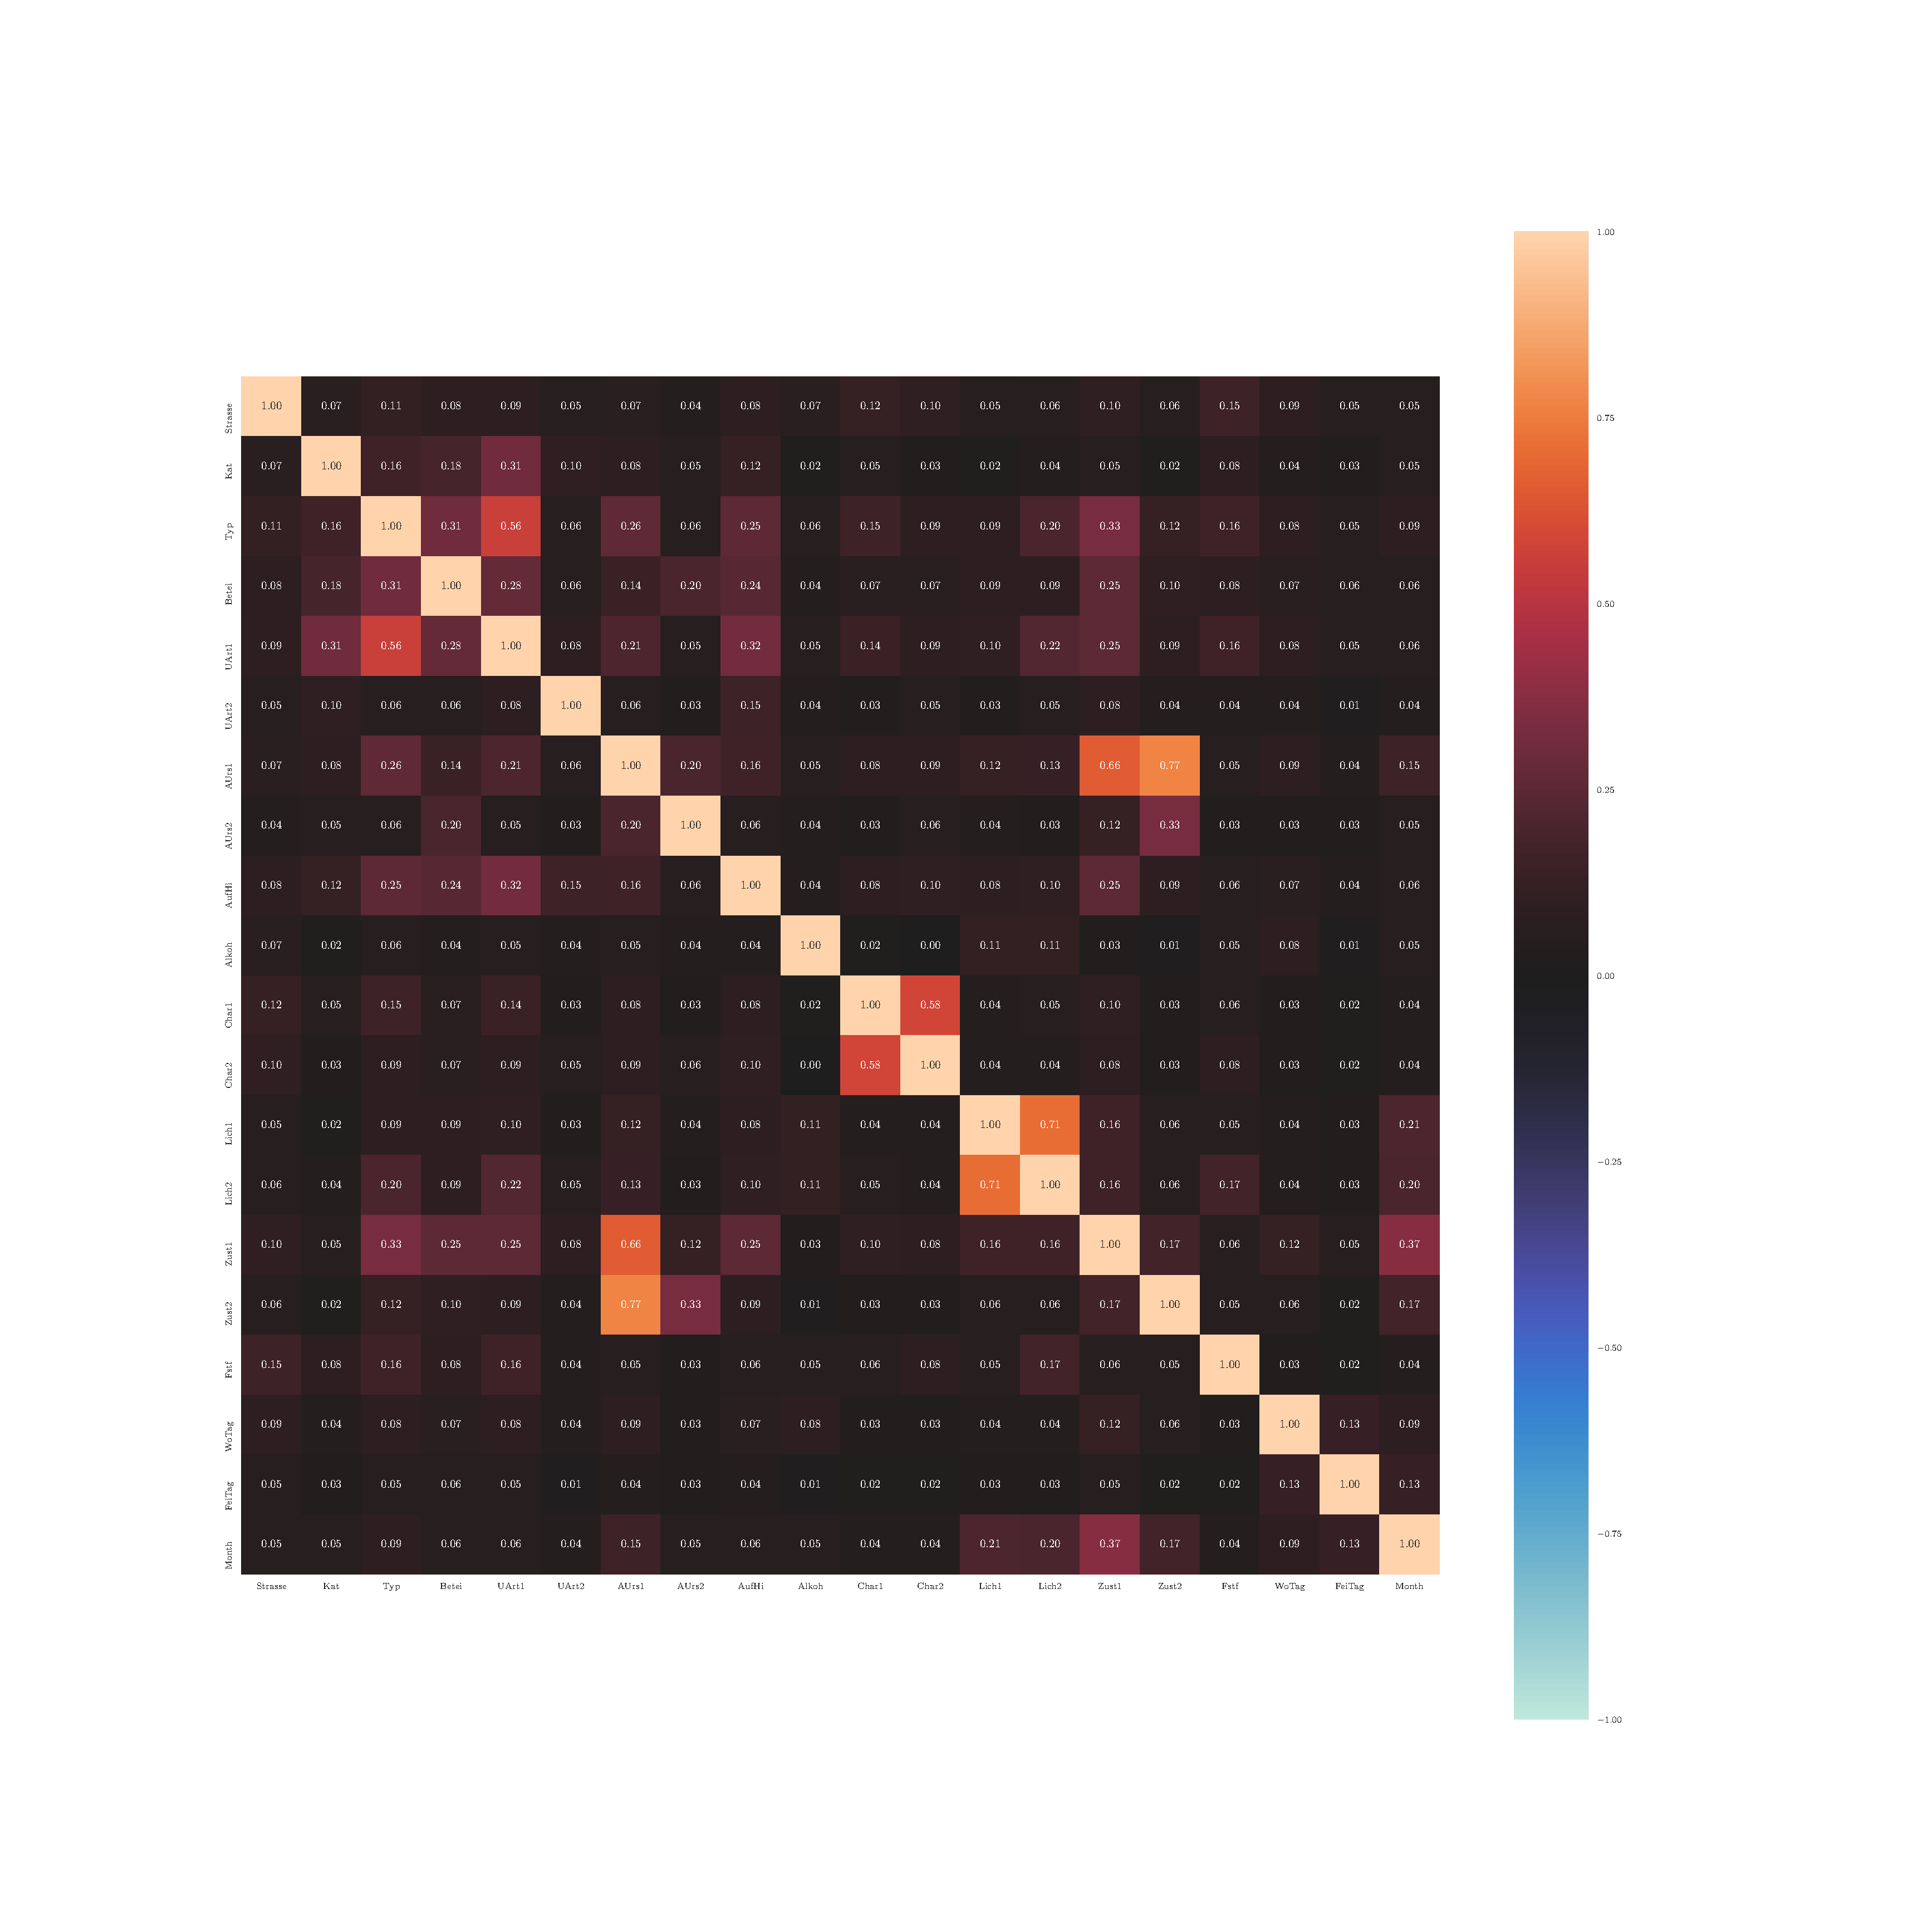
\includegraphics[scale=0.4, trim=4cm 6cm 0cm 6cm]{CorrAnalysis/data/BAYSIS/01_dataset/plots/baysis_dataset_corr_cramers}
% 	\caption{Correlation matrix for BAYSIS dataset, calculated with Cramer's $V$}
% 	\label{img:correlation_matrix_dataset_cramers}
% \end{figure}
% \restoregeometry
% \pagestyle{headings}
% To check for dependent variables which need to be considered in a correlation analysis, the correlation matrix for all relevant parameters in the BAYSIS dataset is calculated for Cramer's $V$. Cramer's $V$ reveals several strong relationships, which are 'Typ'-'UArt1'. 'AUrs1'-'Zust1', 'AUrs1'-'Zust2' and some  trivial relations of 'Char1'-'Char2', 'Bes1'-'Bes2', 'Lich1'-'Lich2'. The results of Theil's $U$ confirms the relationships identified by Cramer's $V$ with a moderate effect size and show the association of 'Aufhi'-'UArt' with a strong effect size. 

% \autoref{tab:baysis_variables} show all categorized parameters, relevant for the correlation analysis, with variable group, type and the format of the containing data. 
% \begin{table}[ht]
% 	\centering
% 	\small
% 	\begin{tabular}{c|c|c|c}
% 		\toprule
% 		\textbf{Variable} 	& \textbf{Group} 	& \textbf{Type} & \textbf{Format} \\
% 		\midrule
% 		Kat  		& categorical 	& ordinal 	& numeric\\
% 		\midrule
% 		Typ 		& categorical 	& nominal	& numeric\\
% 		\midrule
% 		Beteil 		& categorical 	& ordinal	& numeric\\
% 		\midrule
% 		UArt 		& categorical 	& nominal	& numeric\\
% 		\midrule
% 		AUrs 		& categorical 	& nominal	& numeric\\
% 		\midrule
% 		AufHi 		& categorical 	& nominal	& numeric\\
% 		\midrule
% 		Alkoh 		& categorical 	& dichotomous	& numeric\\
% 		\midrule
% 		Char 		& categorical 	& nominal	& numeric\\
% 		\midrule
% 		Bes 		& categorical 	& nominal	& numeric\\
% 		\midrule
% 		Lich 		& categorical 	& ordinal	& numeric\\
% 		\midrule
% 		Zust 		& categorical 	& ordinal	& numeric\\
% 		\midrule
% 		Fstf 		& categorical 	& nominal	& mixed\\
% 		\midrule
% 		WoTag 		& categorical 	& nominal	& text\\
% 		\midrule
% 		FeiTag 		& categorical 	& dichotomous	& numeric\\
% 		\bottomrule
% 	\end{tabular}
% 	\caption{Variable types of \acrshort{baysis} dataset}
% 	\label{tab:baysis_variables}
% \end{table}

The designed evaluation tool, utilizes a PostgreSQL database for its data storage. Therefore the BAYSIS data in form of \acrfull{csv} needs to processed and converted into SQL data entities. Also, the data entities for each accident need to be uniform and comparable with our street network and other entities like roadworks, which makes it necessary to process and map the accidents onto our street network. After the necessary processing and import into the database, 7971 re cords end up being converted and persisted, which equivalent to 77,6\% of the total number of accidents. This 22,4\% of data loss is due to the conversion of from the BAYSIS geo-system to the HERE network, which tries to find a corresponding street network location to the legacy location of the BAYSIS dataset. If it is not able to locate the position of the BYSIS dataset on our street network, the record is discarded.s

\section{Roadwork Data (ArbIS)}
\label{dataset_arbis}

The \acrfull{arbis}, as described in \autoref{dataset_arbis}, is a collection service of all roadworks or maintenance which is planned, ongoing or finished on the Bavarian street network. The dataset for 2019 contains close to 650.000 data-points, which each describe the temporal and spatial extend, road name and number of closed lanes of a roadwork fragment. This fragmentation of events makes is rather hard to statically analyze this dataset since each roadwork is spitted into any number of fragments are only linked by a roadwork identifier. Therefore the analysis of the dataset in this section is rather basic. The import processing works similarly to the \acrshort{baysis} data in \autoref{dataset_baysis} and produces 282.839 roadwork events in the database after the aggregation of fragments. 

With the 4500 long term and more than 40.000 short term building sites on German highways per year \parencite{LAPID2018,Stmi2020}, road construction makes up for the majority of traffic obstructions in the summer months. During the colder month, in which many kinds of construction projects are not possible, snow clearings or long-term constructions are the main obstacles. That also means that the number and type of roadworks varies during the course of a year \parencite{Stmi2020}. 

\begin{figure}[ht]
	\centering
	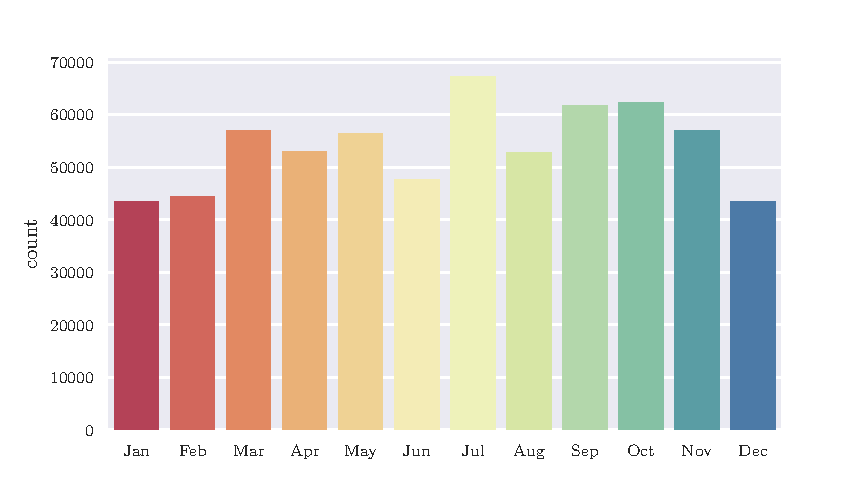
\includegraphics[width=0.7\textwidth]{../CorrAnalysis/data/ArbIS/01_dataset/plots/arbis_dataset_hist_month}
	\caption{Monthly distribution of roadwork fraction counts}
	\label{img:arbis_dataset_dist_month}
\end{figure}

The monthly distribution of roadworks in the year 2019 in figure \autoref{img:arbis_dataset_dist_month} supports this statement, since the winter months of January, February and December tend to have less roadwork that others. The month of July has the most roadworks. Similar to the BAYSIS data the road \textit{A3} and \text{A9} have the highest numbers of roadworks (shown in figure \autoref{img:arbis_dataset_dist_highway}).

\begin{figure}[ht]
	\centering
	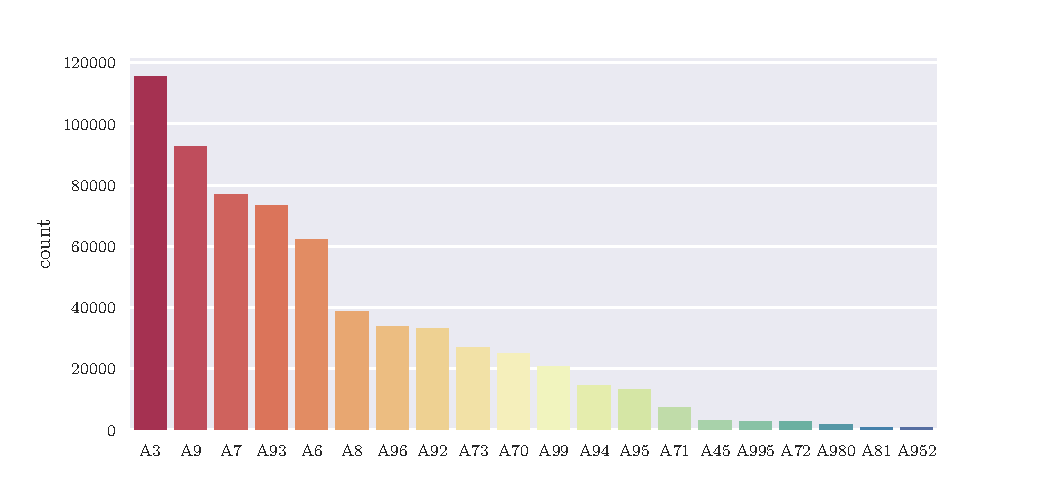
\includegraphics[width=0.7\textwidth]{../CorrAnalysis/data/ArbIS/01_dataset/plots/arbis_dataset_hist_highway}
	\caption{Distribution of roadwork fraction counts, by road}
	\label{img:arbis_dataset_dist_highway}
\end{figure}

\pagebreak

\paragraph{AnzGesperrtFs} refers to the number of closed lanes for the time of the incident. The distribution shows that two states of zero and one block lane hold nearly 100\,\%. Since the variable can be ordered by the number of lane, it is of ordinal type.
\todo{Descriptives}
% \begin{figure}[ht]
% 	\centering
% 	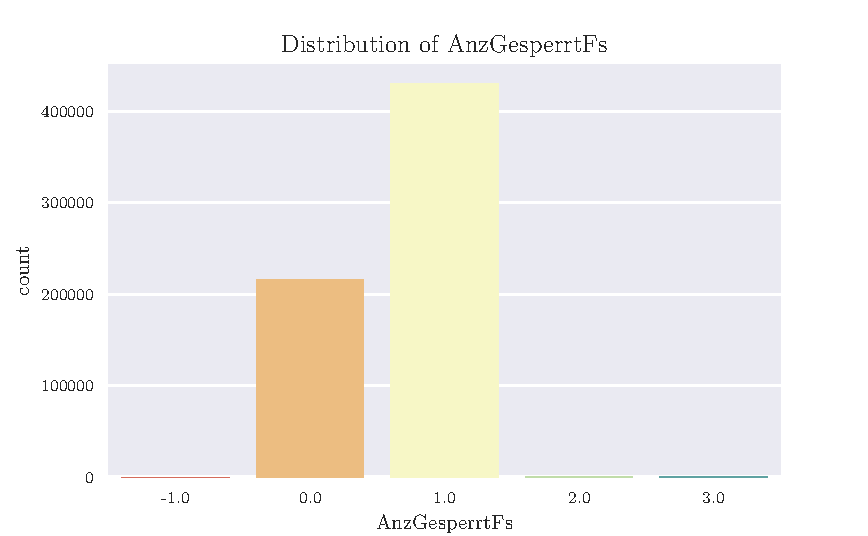
\includegraphics[width=0.7\textwidth]{../CorrAnalysis/data/ArbIS/01_dataset/plots/arbis_dataset_count_AnzGesperrtFs}
% 	\caption{Distribution of roadwork fraction counts, by road}
% 	\label{img:arbis_dataset_count_AnzGesperrtFs}
% \end{figure}

\paragraph{Einzug} describes the shift of the road way due to physical changes, measured in number of lanes. It ranges from one to five lanes, where one, two and five are equally frequent. 
\todo{Descriptives}
% \begin{figure}[ht]
% 	\centering
% 	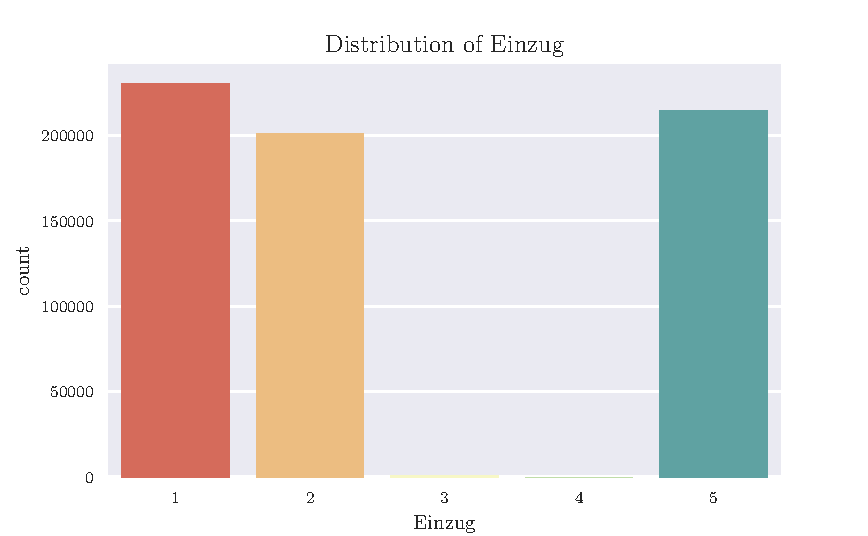
\includegraphics[width=0.7\textwidth]{../CorrAnalysis/data/ArbIS/01_dataset/plots/arbis_dataset_count_Einzug}
% 	\caption{Distribution of roadwork fraction counts, by road}
% 	\label{img:arbis_dataset_count_Einzug}
% \end{figure}

\paragraph{Length} is calculated from the two dataset parameters \textit{VonKilometer} and \textit{BisKilometer}, since it is not part of the original ArbIS dataset. 
\todo{Descriptives}

\paragraph{Duration} is calculated from the two dataset parameters \textit{Von} and \textit{Bis}, since it is not part of the original ArbIS dataset.
\todo{Descriptives}

%\autoref{table:baysis_variables} show all categorized parameters, relevant for the correlation analysis, with variable group, type and the format of the containing data.	
% \begin{table}[ht]
% 	\centering
% 	\begin{tabular}{c|c|c|c}
% 		\toprule
% 		\textbf{Variable} 	& \textbf{Group} 	& \textbf{Type} 		& \textbf{Format} \\
% 		\midrule
% 		AnzGesperrtFs  	& categorical 	& ordinal 	& numeric\\
% 		\midrule
% 		Einzug  		& categorical 	& ordinal 	& numeric\\
% 		\midrule
% 		Length  		& continuous 	& interval 	& numeric\\
% 		\midrule
% 		Duration  		& continuous 	& interval 	& numeric\\
% 		\bottomrule
% 	\end{tabular}
% 	\caption{Variable types of \acrshort{baysis} dataset}
% 	\label{table:arbis_variables}
% \end{table}

\chapter{Methodology of processing}
\label{methodology}
The previous chapters provided an introduction into the systems, data and methods which will be used to determine if jams characteristics, detected in \acrshort{fcd} and incident characteristics from accidents (\acrshort{baysis}) and roadworks (\acrshort{arbis}) are statistically related to each other. The research question to be answered stands as follows:

\begin{center}
	\textit{Do congestion- and incident-characteristics correlate?}
\end{center}

\medskip

The methodology to answer these research questions, will be elaborated in this chapter, starting with the detection of jams in the FCD. This also contains the generation of congestion characteristics and collection of adjacent incident. The \acrshort{fcd} is a continuous time series of datapoint which represents the mean absolute and relative speed of the street section at each 3-minute interval on a road section. In \ref{dataset_fcd} we determined that thought a manual visual analysis jams can be easily identified. This manual identification will be automated because of the amount of data representing a complete year and all Bavarian highways. The gathered tuples of congestion and incident are then processed and exported into a unified data-structure. 

The \gls{evaltool} from the \gls{congstats} service, the project which inspired this thesis, was developed for this purpose and will be expanded with required features. Afterward the stored dataset of congestion and incidents events will be analyzed for correlations and other statistic indicators.

\bigskip

\section{Detection Algorithm}
\label{methodology_detection}
First step is the detection of congestion events. The definition in \ref{definition_congestion} states that a congestion is a dense, timely and spatial accumulation of jammed cells, also describable as cluster of jammed cells. Therefore a clustering algorithm would be suitable to identify congestion events.

For the classification of the congestion events into different types, by theirs spatial and timely extends a shaping algorithm is needed. It is supposed to convert the accumulation of cells into a simple describable shape, which can be put into groups.

\subsection{Clustering of Floating-Car-Data}
\label{methodology_detection_clustering}
The term clustering is the short form of a data mining technique also called numerical taxonomy or cluster analysis with the goal of finding data structures or associations. For this purpose a multitude of algorithms where developed over time, varying in they strategies, methods and performance \parencite{Busch2004}. For example k-means or k-metoid (point distance), affinity propagation (graph distance), mean-shift (point distance), DBSCAN (nearest point distance), gaussian mixtures (mahalanobis distance to centers) or spectral clustering (graph distance), which can be sorted into the categories of partition-based, hierarchical-based and density-based clustering \parencite{Chauhan2020,Yildirim2020}.

% https://texample.net/tikz/examples/probability-tree/
% https://webis.de/downloads/theses/papers/busch_2005.pdf 1.6
%\begin{tikzpicture}[grow=right, sloped]
%\node[bag] {Cluster Algorithms}
%    child {
%        node[bag] {hierarchic}        
%             child {
%                node[end, label=right:
%                    {single-linkage, group-average}] {}                
%                edge from parent
%            }         
%            edge from parent 
%    }
%    child {
%        node[bag] {iterative}        
%            child {
%                node[end, label=right:
%                    {k-means, k-metoid, Kerninghan-Lin}] {}                
%                edge from parent
%            }         
%            edge from parent 
%    }
%    child {
%        node[bag] {density-based}        
%            child {
%                node[end, label=right:
%                    {DBSCAN, MajorClust}] {}                
%             	edge from parent
%            }
%            edge from parent
%    }
%	child {
%        node[bag] {meta-search}        
%                 child {
%                node[end, label=right:
%                    {genetic algorithms}] {}
%                edge from parent
%            }            
%            edge from parent
%    }
%    child {
%        node[bag] {statistical}        
%        child {
%                node[end, label=right:
%                    {gaussian mixtures}] {}
%                edge from parent
%            }
%            edge from parent         
%    };
%\end{tikzpicture}

\bigskip

\begin{figure}[ht]
	\centering
	\includegraphics[scale=0.5]{images/cluster_seperate.png}
	\caption{Example clustered by k-means algorithm \parencite{Yildirim2020}}
	\label{cluster_kmeans}
\end{figure}

To illustrate which problems can occur when using cluster algorithms and to defined the features which makes algorithm suitable, the k-means is used as base comparison. The figure \ref{cluster_kmeans} shows three differently colored groups of points, which are clustered into three clusters, represented by the circles around the groups. It demonstrates the general principle of clustering and was done by the common k-means algorithm with the $a$ $priori$ parameter of three clusters. 

\begin{figure}[ht]
	\centering
	\includegraphics[scale=0.4]{images/cluster_1.png}
	\includegraphics[scale=0.4]{images/cluster_2.png}
	\includegraphics[scale=0.4]{images/cluster_3.png}
	\caption{Example clustered by density-based algorithm \parencite{Yildirim2020}}
	\label{cluster_dbscan}
\end{figure}

This works well as long as the groups don't overlay, intersect or have arbitrary shapes like in the figures \ref{cluster_dbscan}. When this is the case, the k-mean may cluster loosely related point together, which actually are more strongly related to other points, because it considers every point as possible neighbor. Since jams in FCD data can overlay and have any number of shape, as suitable algorithms need to be able to handle such data.

Another issue with many clustering algorithms is the increasing runtime when processing larger amounts of data. The objective function \ref{formula_kmeans} of the exemplary k-mean states that $n$ distances are calculated for $k$ points \parencite{Santhanam2010}. With the assumption that every distance for every point will be calculated and therefore $k=n$, the Big $\Theta$ notation, commonly known as Big $O$, describing the scaleable time complexity of an algorithm, is $O(n \cdot K \cdot I \cdot d)$ ($n$ = number of points, $K$ = number of clusters, $I$ = number of iterations, $d$ = number of attributes) \parencite{Dalatu2016}. It is commonly simplified in literature to $O(n^2)$, a quadratic complexity \parencite{Pakhira2014}. The assumption also entails that in a worst case scenario $n^2$ calculations have to be computed over all iterations.

\begin{equation}
\label{formula_kmeans}
	k_{mean} =  \sum_{j=1}^k{\sum_{i=1}^n{\abs{x_i^j-c_j}}}
\end{equation}

\bigskip

A Big $O$ notation of $O(n^2)$ can generally be described as inefficient, but if we would apply the worst case scenario as an example on the data of the highway A3 and a timeframe of 24 hours, which contains 836.752 data points, the runtime issue becomes quite obvious. As the equation \ref{equation_kmeans_nn} show, the total number of calculation is quite high, resulting in a considerable runtime. \parencite{Busch2004}

\begin{equation}
\label{equation_kmeans_nn}
	 = 836752 \cdot 836752 = 700.153.909.504 = 7 \cdot 10^{11}
\end{equation}

\bigskip

Entering density-based methods, which are better suited to identify distinctive, arbitrary clusters in, by looking for a contiguous region of high point density, separated from others by contiguous regions of low point density \parencite{Chauhan2020}. These do not necessarily have less runtime, but better cluster representation.

\subsubsection{Density Clustering Algorithm}
The DBSCAN algorithm, standing for \textbf{d}ensity-\textbf{b}ased \textbf{s}patial \textbf{c}lustering of \textbf{a}pplications with \textbf{n}oise, is able to find arbitrary shaped cluster and clusters by considering the spatial density, which also represents noise. The basic idea of this algorithm is to form cluster of points, which are close too \textbf{many} other points of the cluster. For this strategy two thresholds parameters are needed. The first being the minimal size of a cluster, referred to as $MinPts$, which defines the minimum number of points necessary to form a cluster. And secondly the maximum distance threshold between points, $eps$ ($\varepsilon$), to be considered as neighbors and become part of a cluster. These thresholds classify a data point as core point, (directly) density-reachable point or noise. \parencite{Yildirim2020,Chauhan2020,Padro2017}

\begin{itemize}
	\item A \textbf{core} point $q$ has at least $MinPts$ points around them within the neighborhood $\varepsilon$, including itself.
    \item \textbf{Directly density-reachable} border points have at least one core point within the neighborhood $\varepsilon$.
     \item \textbf{Density-reachable} border points have at least one core point within the neighborhood $\varepsilon$ of a cain of points $p_1,p_2,...p_n$.
 	\item \textbf{Noise} or outliner point are neither core points nor are they density-reachable and therefore have less than $MinPts$ in their neighborhood $\varepsilon$, including itself.
\end{itemize}

The general procedure of the algorithm is as follows \parencite{Zhao2018}, with the input of $n$ points, neighborhood radius $\varepsilon$ and density threshold $MinPts$:

\begin{itemize}
	\item[\textbf{1.}] Mark all points as \textit{unvisited}
	\item[\textbf{2.}] Choose point $p$ randomly from all \textit{unvisited} points.
	\begin{itemize}
		\item[\textbf{a.}] Choose point $p$ randomly from all \textit{unvisited} points and mark $p$ as \textit{visited}.
		\item[\textbf{b.}] Count points in the neighborhood $\varepsilon$ to check if $p$ is core point. If $p$ is core point, create new cluster $C$ and add all directly density-reachable and \textit{unvisited} points. Otherwise mark $p$ as noise.
		\item[\textbf{c.}] Choose point $p'$ randomly from all \textit{unvisited} points of $C$ and mark $p$ as \textit{visited}.
		\item[\textbf{d.}] Count points in the neighborhood $\varepsilon$ to check if $p'$ is core point. If $p$ is core point add all directly density-reachable points, which do not already belong to a cluster, to $C$. Otherwise mark $p$ as noise.
		\item[\textbf{e.}] Repeat \textbf{c} and \textbf{d} until there are no \textit{unvisited} points left in $C$.	
	\end{itemize} 
	\item[\textbf{3.}] Repeat \textbf{2} until all points are \textit{visited} 
\end{itemize}

%https://www.kde.cs.uni-kassel.de/wp-content/uploads/ws/LLWA03/fgml/final/Kirchner.pdf
%https://www.researchgate.net/publication/322729622_Characterizing_Diffusion_Dynamics_of_Disease_Clustering_A_Modified_Space-Time_DBSCAN_MST-DBSCAN_Algorithm
%https://www.nature.com/articles/s41598-017-12852-z
%http://citeseerx.ist.psu.edu/viewdoc/download?doi=10.1.1.63.1629&rep=rep1&type=pdf
%http://cucis.eecs.northwestern.edu/publications/pdf/HAL18.pdf

\subsubsection{Artificial Distance Measuring}
The algorithm is based on the density of points. This density representation is achieved via checking the neighborhood $\varepsilon$ against calculation of distance from point $A$ to $B$, typical the Euclidean distance, which is based on the pythagorean theorem (see equation \ref{formula_euclidean} \parencite{Erhard2020}).

\begin{figure}[ht]
	\centering
	\begin{tikzpicture}[scale=0.7]
			
		\draw [<->,thick] (0,5) node (yaxis) [above] {$y$}
	        |- (10,0) node (xaxis) [right] {$x$};
	        
	    \foreach \x in {1,...,9}
	    	\draw[black!30] (\x,0) -- (\x,5);
	    	
	   	\foreach \y in {1,...,4}
	    	\draw[black!30] (0,\y) -- (10,\y); 
	        
	    \foreach \x in {1,...,9}
	    	\draw (\x,1pt) -- (\x,-3pt)
			node[anchor=north] {\x};
			
		\foreach \y in {1,...,4}
	    	\draw (1pt,\y) -- (-3pt,\y) 
	     	node[anchor=east] {\y}; 
	
		\coordinate[label={270:$ $}] (C) at (8,1);
		\coordinate[label={180:$A$}] (A) at (2,1);
		\coordinate[label={30:$B$}] (B) at (8,4);
	
		\draw (C) -- (A)node[midway,below left]{$a$} -- (B)  -- cycle node[midway,below right]{$b$};
	       
		\draw [dashed] (C) -- ($(A)!(C)!(B)$) coordinate (P) node [midway, left]{$h$};
		
		\draw[decorate,decoration={brace,raise=12pt,amplitude=5pt}] (A) -- (B);
		
		\path (B) -- (P) node[midway,above]{$$} -- (A) node[midway,above]{$$} ($($(A)!0.5!(B)$)!1.2cm!90:(B)$) node {$d_{A,B}$}; % You can nest calc syntax!
		
		\filldraw[fill=white] (C) -- ($(C)!2mm!(A)$) coordinate (U) -- ($(U)!2mm!90:(C)$) 
	      --($(C)!2mm!(B)$) --cycle;
		
		\draw ($(P)!2mm!(C)$) coordinate (V) -- ($(V)!2mm!90:(C)$) --($(P)!2mm!(B)$);

	\end{tikzpicture}
	\caption{Euclidian distance in 2-dimensional euclidian space}
\end{figure}

\begin{equation}
	d_{A,B} = \sqrt{a^2 + b^2} = \sqrt{(x_B-x_A)^2+(y_B-y_A)^2}
	\label{formula_euclidean}
\end{equation}

\medskip

As shown above, the euclidean distance calculation assumes a Euclidean space, meaning equal scaling of both axis, which is not the case with FCD. The 2D-space of the FCD is defined by a spatial and a temporal dimension, which are scaled differently as mentioned in section \ref{dataset_fcd}. The vertical axis shows the temporal dimension is regular scales in 3 minute intervals. The horizontal axis is the spatial extend, scaled in one cell per step, representing one road link (road link are rather small subsection of roads, defining the course), which vary heavily in their length. This can be visualized like:

\begin{figure}[ht]
	\centering	
	\begin{tikzpicture}[scale=0.7]	
	
		\draw [<->,thick] (0,5) node (yaxis) [above] {$y$}
	        |- (10,0) node (xaxis) [right] {$x$};
	    % X Axis lines  
	    \draw[red] (0.7,1pt) -- (0.7,-3pt)
		node[anchor=north] {70}; 
	    \draw[red] (1.5,1pt) -- (1.5,-3pt)
		node[anchor=north] {110};   
	    \draw[red] (2.5,1pt) -- (2.5,-3pt)
		node[anchor=north] {250};
		\draw[red] (4,1pt) -- (4,-3pt)
		node[anchor=north] {400};
		\draw[red] (7,1pt) -- (7,-3pt)
		node[anchor=north] {700};
		\draw[red] (8.3,1pt) -- (8.3,-3pt)
		node[anchor=north] {830};
		\draw[red] (9.3,1pt) -- (9.3,-3pt)
		node[anchor=north] {930};
	    \foreach \x in {0.7,1.5,2.5,4,7,8.3,9.3}
	    	\draw[black!30] (\x,0.1) -- (\x,4.9);
	    % Y Axis lines	
		\draw[red] (1pt,1) -- (-3pt,1) 
	     	node[anchor=east] {3}; 
	    \draw[red] (1pt,2) -- (-3pt,2) 
	     	node[anchor=east] {6}; 
	    \draw[red] (1pt,3) -- (-3pt,3) 
	     	node[anchor=east] {9}; 
	    \draw[red] (1pt,4) -- (-3pt,4) 
	     	node[anchor=east] {12}; 
	    \foreach \y in {1,...,4}
	    	\draw[black!30] (0.1,\y) -- (9.9,\y); 
	    	
	    \coordinate[label={270:$ $}] (C) at (7,1);
		\coordinate[label={180:$A$}] (A) at (1.5,1);
		\coordinate[label={30:$B$}] (B) at (7,4);
	
		\draw (C) -- (A)node[midway,below left]{$a$} -- (B)  -- cycle node[midway,below right]{$b$};
	       
		\draw [dashed] (C) -- ($(A)!(C)!(B)$) coordinate (P) node [midway, left]{$h$};
		
		\draw[decorate,decoration={brace,raise=12pt,amplitude=5pt}] (A) -- (B);
		
		\path (B) -- (P) node[midway,above]{$$}-- (A) node[midway,above]{$$} ($($(A)!0.5!(B)$)!1.2cm!90:(B)$) node {$d_{A,B}$}; % You can nest calc syntax!
		
		\filldraw[fill=white] (C) -- ($(C)!2mm!(A)$) coordinate (U) -- ($(U)!2mm!90:(C)$) 
	      --($(C)!2mm!(B)$) --cycle;
		
		\draw ($(P)!2mm!(C)$) coordinate (V) -- ($(V)!2mm!90:(C)$) --($(P)!2mm!(B)$);
				
	\end{tikzpicture}
	\caption{Euclidian distance in 2-dimensional non-euclidian space}
\end{figure}

\bigskip

This makes a direct application of the Euclidian distance invalid to calculate the distance from point $A$ to point $B$. But then how can distances be represented in this 2D-space with different units? The solution developed for this application is to expand the 2D-representation of time and space into a 3D-representation of time, space and speed (absolute mean traveling speed is part of \acrshort{fcd}, see section \ref{dataset_fcd}). Because speed $[km/h]$ consist of both time $[min]$ and space $[m]$ is allows for the introduction of the common unit travel time, which can be comprise from these three parameters traveling speed, time duration and link length. At this point it has to be noted, the implemented definition does not represent actual travel time but server the need of being common unit and rough representation. To separate both terms the term \textit{artificial travel time} will be used instead of \textit{travel time}.

\begin{figure}[ht]
	\centering	
	\begin{tikzpicture}
	
		\begin{axis}[
			view={120}{40},
			width=220pt,
			height=220pt,
			grid=major,
			z buffer=sort,
			xmin=1,xmax=9,
			ymin=1,ymax=9,
			zmin=1,zmax=9,
			enlargelimits=upper,
			xtick={1,...,9},
			ytick={1,...,9},
			ztick={1,...,9},
			xlabel={$time$},
			ylabel={$link$},
			zlabel={$speed$},
			point meta={x+y+z+3},
			colormap={summap}{
				color=(black); color=(blue); 
				color=(black); color=(white) 
				color=(orange) color=(violet) 
				color=(red)
			},
			scatter/use mapped color={
				draw=mapped color,fill=mapped color!70},
			]
			% http://pgfplots.sourceforge.net/gallery.html. 
		\end{axis}
		
	\end{tikzpicture}
	\caption{3-dimensional space representation of \acrshort{fcd}}
\end{figure}

Assuming an 3D-space of $time steps$ $\equiv x=[x_1,...,x_n]$ , $space$ $\equiv y=[y_1,...,y_n]$ and $speed$ $\equiv z=[z_1,...,z_n]$ the mathematical definition of calculation for the distance from point $A$ to point $B$ is as follows.

\paragraph{Time dimension} Traveling just in the time dimension is not actual possible, hence the term artificial travel time. But assuming that both point $A$ and $B$ are at the same \textbf{space} step, the distance is calculated by:

\begin{equation}
	t_{x,A,B}^{artificial} = (x_B - x_A) \cdot ( x_{interval} + 1 )
	\label{equation_t_v_time}
\end{equation}

\begin{itemize}
	\setlength\itemsep{0.1em}	
	\item[] $x_A | x_B$ is the $x$ index of point $A | B$
	\item[] $x_{interval}$ is the time interval or step duration
\end{itemize}

\paragraph{Space dimension} Traveling just through space is also not actual possible, but in the artificial travel time. Under the assumption that point $A$ and point $B$ are in the \textbf{time} step, the distance is calculated by:  

\begin{equation}
	t_{y,A,B}^{artificial} = (\frac{y_{A}^{length}}{2}  \cdot z_{A}^{speed}) + (\frac{y_{B}^{length}}{2} \cdot z_{B}^{speed}) + \sum_{i}^{y_A + 1,...,y_B - 1} (y_{i}^{length} \cdot z_{i}^{speed})
\end{equation}

\begin{itemize}
	\setlength\itemsep{0.1em}	
	\item[] $y_A | y_B$ is the $y$ index of point $A | B$
	\item[] $y_{length}$ is the length of the link
	\item[] $z_{speed}$ is the speed in the cell
\end{itemize}

\paragraph{Diagonal time/space dimension} The diagonal distance or time/space distance is based on the concept of the Euclidian distance. Although the conversion to the artificial travel time fixes the disparity of the axis units, a calibration for weighing the time and space axis is still necessary. This achieved by using the aimed gap thresholds to form a calibrator value, which scales the axis appropriately, to be of equal scaling (see source code ??). This makes it possible to use the artificial travel time a distance parameters, for horizontal, vertical and diagonal movements.

\begin{equation}
	t_{x,y,A,B}^{artificial} = \sqrt{(t_{x,A,B}^{art})^2 + (t_{y,A,B}^{art} \cdot c)^2}
\end{equation}
\begin{equation}
	v_{A,B}^{mean} = \sum_{ij}^{xy_A + 1,...,xy_B - 1} z_{ij}^{speed}
\end{equation}
\begin{equation}
	c = \frac{t_{min,gap} \cdot v_{freeflow}}{l_{min,gap}}
\end{equation}

\begin{itemize}
	\setlength\itemsep{0.1em}	
	\item[] $xy_A | xy_B$ is the $xy$ index of point $A | B$
	\item[] $z_{speed}$ is the speed in the cell
	\item[] $v^{mean}$ is mean speed in the area between $A$ and $B$
	\item[] $c$ is the time-space calibrator
	\item[] $t_{min,gap}$ is the the aimed time gap
	\item[] $l_{min,gap}$ is the the aimed space gap
	\item[] $v_{freeflow}$ is the assumed free flowing speed (typically 130\,[km/h])
\end{itemize}

% TODO read and add infos: https://diglib.tugraz.at/download.php?id=576a764ebc982&location=browse \parencite{Hatbauer2011}

\subsubsection{Performance Tuning}
Leaving out the runtime implication of the distance measurer, the complexity of DBSCAN clustering algorithm can be as low as $O(nlog_n)$. This best case scenario can be achieved by using indexing system to store the clustering data in a space representation, like a 2D-Tree. This reduces the number of point to check for neighborhood, from all points in a worst case scenario (equivalent to a complexity of $O(n^2)$), to just adjacent points \parencite{Chauhan2020}. For initially testing a $kd$-Tree was implemented, which stores data points as leafs in a tree, where the nodes divide the space consecutively in the $x$ and $y$ dimension \parencite{Hucker2020,Dalitz2009}. This improved the runtime performance, but also added complexity, which endorsed the use of a natively implemented data structure, like the TreeMap. The TreeMap strictly speaking is no a 2D-Tree, but has an average complexity of $O(nlog_n)$ and be used as a 2D-Tree by filtering with two parameters (see source code ??). \parencite{Baeldung2020_1,Baeldung2020_2}

% https://de.wikipedia.org/wiki/K-d-Baum
% https://github.com/jmhodges/kdtree2/blob/master/doc/kdtree2.tex

To further accelerate the algorithm, is is implemented with support of parallel computation or threading, which allows the executing Java VM to used multiple CPU cores and run multiple processes in parallel.

\subsubsection{Calibration}
Parameter calibration and estimation is a vital task when implementing algorithms. The DBSCAN uses the neighborhood $\varepsilon$ and $minPoints$ parameters as adjustments. If $\varepsilon$ is too small, part of the data will not be clustered, since the distances to many points is below the threshold. These points are therefore considered as outliner/noise and reduce the actual size of the cluster or make the cluster neglect able because $minPoints$ will not be reached to create a dense region. On the other side, if the value is chosen too high, a high number of point will be considered as one cluster, when they should be multiple separate clusters. The $minPoints$ threshold should generally satisfy $minPoints > D + 1$ and should be high enough for our implementation to neglect small and arbitrary jams. \parencite{Padro2017}. For the implemented variation of distance measuring the aimed time gap $t_{min,gap}$ and aimed space gap $l_{min,gap}$ threshold also need to be set. This is necessary to scale the axis so that they represent the aimed thresholds through neighborhood $\varepsilon$. The following values are the result of iterative testing, to find the most representable cluster consolidation results. 

\begin{itemize}
	\item Aimed spatial gap : $l_{min,gap} = 5000 \, [m]$
	\item Aimed temporal gap : $t_{min,gap} = 6 \, [min]$
	\item Virtual travel-time gap $\varepsilon = t_{min,gap}^{artificial} = 360 \, [s]$
\end{itemize}

\subsection{Pre and Post Data Revision}
Datasets are rarely flawless and as mentioned in section \ref{dataset_fcd}, the provided FCD dataset has some defects. To reduce these defects before the clustering, static speed blocks are removed as pre-processing measure. When the speed is consistent in a a continuous time and space extent, we assume that the data block is flawed because of the implausible consistent speeds. (see source code ??) 

As post processing, clusters which are too short in duration and length are removed. We assume that below a threshold a cluster can not be considered as a jam, and should be neglected. The following values for the minimal duration and length of a congestion where used. (see source code ??)

\begin{itemize}
	\item Minimum spatial length of an congestion event : $l_{min} = 1000 \, [m]$
	\item Minimum temporal duration of an congestion event : $t_{min,gap} = 9 \, [min]$
\end{itemize}

\subsection{Shaping}
\label{methodology_detection_shaping}
For a shape representation of the congestion the geometric method of convex hull was implemented. This shape was initially intended to be the base for the classification of congestion event into different type of jams alongside the paper \textit{Automated Classification of Different Congestion Types} \parencite{Kessler2020}. Unfortunately this classification processing was not finished in time for this thesis, but the implementation found use in the visual representation of jams and characteristics calculation.

%https://www.diva-portal.org/smash/get/diva2:931027/FULLTEXT02
% \begin{figure}[ht]
% 	\centering
% 	\begin{tikzpicture}
%   	\draw (0,0) -- (0,1) -- (2,2) -- (2,0) -- cycle;
%   	\foreach \point in {(0,0),(1,1),(2,2),(0,1),(2,0)} {
%     	\fill[black] \point circle[radius=1pt];
%   	}
% 	\end{tikzpicture}
% \end{figure}
% TODO expand

\section{Matching Algorithm}
\label{methodology_matching}
The matching process for finding adjacent incidents around jams is rather simple. When iterating over all jams, the incidents located on the same road and on the same day are evaluated for the temporal and spatial distance to the outer line of the the congestion. When the distance falls in the range of the threshold they are considered as adjacent. The following values where used as thresholds.

\begin{itemize}
	\item The spatial distance an adjacent incident : $l_{min,dist} = 2000 \, [m]$
	\item The temporal distance an adjacent incident : $t_{min,dist} = 25 \, [min]$
\end{itemize}

\section{Data Processing}
\label{methodology_data_processing}
As result of the previous detection a matching algorithms we now have a list of jams with spatial and timely adjacent incidents (accidents and roadworks). For further analysis congestion and incident matches will be expanded with additionally features and exported in to a local data format for the analysis.

\subsubsection{Congestion}
For the analysis we are interested in the length and duration of the congestions. The length and duration of congestions, defined by the boundary rectangle can be heavily biased. It is also a very rough representation of the extends, and is therefore considered to be the maximum length and maximum duration. To have another representation of the time and space extends, an average duration and length is calculated. This is done by iteration over the time step or link step and calculating the mean of the jam length or duration respectively.

For the analysis of social impact the congestion object is expanded with a time loss estimation, differentiated for passenger cars and heavy goods vehicles (HGV). This part was not implemented by the writer, but from the mentor Stefan Gürtler (S\&W) and used as implemented. Since it is used in the analysis, the calculation will explained in the following. First the headway with the cell speed is calculated with the assumption that drivers follow the two second rule, see \cref{equation_timeloss_vehicles_headway}.
\begin{equation}
	l_{headway} = 2 \cdot \frac{v_{cell}}{3600}
	\label{equation_timeloss_vehicles_headway}
\end{equation}
Then the occupied space of a hundred vehicles can then be comprised by the headway and the vehicle lengths as in \cref{equation_timeloss_vehicles_length}.
\begin{equation}
	l_{100,vehicles} = n_{car} \cdot (l_{headway} \cdot l_{car}) + n_{hgv} \cdot (l_{headway} \cdot l_{hgv})
	\label{equation_timeloss_vehicles_length}
\end{equation}
\begin{equation}
	n_{car} = (1-r) \cdot 100
\end{equation}
\begin{equation}
	n_{hgv} = r \cdot 100 
\end{equation}
The density of vehicles for the cell speed can be calculated as in \cref{equation_timeloss_vehicles_density}.
\begin{equation}
	d = \frac{1}{((1-r) \cdot (l_{headway} \cdot l_{car}) + r \cdot (l_{headway} \cdot l_{hgv})}
	\label{equation_timeloss_vehicles_density}
\end{equation}
The appropriate vehicle count can then be deviated by \cref{equation_timeloss_vehicles_count,equation_timeloss_vehicles_count_car,equation_timeloss_vehicles_count_hgv}
\begin{equation}
	n_{vehicles} = l_{cell} \cdot d
	\label{equation_timeloss_vehicles_count}
\end{equation}
\begin{equation}
	n_{car} = (1-r) \cdot n_{vehicles}
	\label{equation_timeloss_vehicles_count_car}
\end{equation}
\begin{equation}
	n_{hgv} = r \cdot n_{vehicles}
	\label{equation_timeloss_vehicles_count_hgv}
\end{equation}
To calculate the total hours lost for either passenger car or heavy goods vehicle due to the jam, \cref{equation_timeloss} is applied with the appropriate 
\begin{equation}
	t_{loss,car/hgv} = n_{car/hgv} \cdot n_{lanes} \cdot l_{cell} \cdot ( v_{free} - v_{cell})
	\label{equation_timeloss}
\end{equation}
\begin{itemize}
	\setlength\itemsep{0.01em}	
	\item[] $v_{cell}$ is the mean vehicle speed in [km/h]
	\item[] $v_{free}$ is the assumed free flowing speed in [km/h]
	\item[] $d$ is the density of vehicles in the cell [veh/km]
	\item[] $r$ is the ratio of heavy goods vehicle to passenger cars 
\end{itemize}

\bigskip

A analysis based on all matched could be heavily biased, because all kind of relations are considered a once. To do a more specialized analysis, the congestion incident matches should be categorized. The three categories to be evaluated separately can be described as \textit{Initiator}, \textit{Effector} and \textit{Follower}.
\begin{itemize}
	\setlength\itemsep{0.1em}	
	\item[] \textbf{Jam Initiator} are matches, where the incidents happened before or immediately at the beginning of a congestion. These could be the initiator or cause for the congestion and are therefore the most interesting to analysis.
	\item[] \textbf{Jam Effector} are matches, where the incidents happened during a congestion or overlaps with the congestion. These probably have the jam as a cause, like rear-end accidents.
	\item[] \textbf{Jam Follower} are matches, where the incidents happened after the congestion. 
\end{itemize}

% \begin{figure}[ht]
% 	\centering	
% 	\begin{tikzpicture}
% 		\draw[pattern=north west lines, pattern color=blue] (0,0) rectangle (2,4);

% 		\draw[fill=fondo,very thick] (0:1 cm) -- (72:1 cm) -- (144:1 cm) -- (216:1 cm) -- (288:1 cm) -- cycle;
% 		\foreach \x in {0,72,...,288} {
% 			\draw[diagonal,thin] (\x:1 cm) -- (\x + 180:0.809 cm);}

% 	\end{tikzpicture}
% 	\caption{Euclidian distance in 2-dimensional non-euclidian space}
% \end{figure}

To be able to run the categorization after the runtime intensive detection and matching processing, four additional congestion parameters are introduced. They describe the relative location of the incident to the congestion event. The temporal reference of the incident to the congestion is described by the parameter \textbf{temporalGlobalLocation}, based on the temporal distance. 
\begin{table}[ht]
	\centering
	\begin{tabular}{c|l}  
		1 & is before \\ 
 		2 & is overlapping before \\ 
 		3 & is during \\
 		4 & is overlapping after \\
 		5 & is after \\
	\end{tabular}
	\caption{Encoding and description of temporal global location reference}
	\vspace{-4mm}
\end{table}

The spatial reference of if the incident to the congestion is described by the parameter \textbf{spatialGlobalLocation}, based on the spatial distance.
\begin{table}[ht]
	\centering
	\begin{tabular}{c|l}  
		1 & is before \\ 
 		2 & is during or overlapping \\ 
 		3 & is after \\ 
	\end{tabular}
	\caption{Encoding and description of spatial global location reference}
	\vspace{-4mm}
\end{table}

In the case that the incident happened temporal  during the congestion. The (\textbf{temporalInternalLocation} parameter is set. It describes in more detail where the incident is located during the congestion.
\begin{table}[ht]
	\centering
	\begin{tabular}{c|l}  
		1 & 10\,\% to Beginning \\
 		2 & 10\,\% - 30\,\% to Beginning \\
 		3 & 30\,\% - 70\,\% (Middle) \\
 		4 & 30\,\% - 10\,\% to Ending \\
 		5 & 10\,\% to Ending \\
	\end{tabular}
	\caption{Encoding and description of temporal internal location reference}
	\vspace{-4mm}
\end{table}

In the case that the incident happened spatial during the congestion. The \textbf{spatialInternalLocation} parameter is set. It describes in more detail where the incident is located during the congestion.
\begin{table}[ht]
	\centering
	\begin{tabular}{c|l}  
		1 & 10\,\% to Beginning \\
 		2 & 10\,\% - 30\,\% to Beginning \\
 		3 & 30\,\% - 70\,\% (Middle) \\
 		4 & 30\,\% - 10\,\% to Ending \\
 		5 & 10\,\% to Ending \\
	\end{tabular}
	\caption{Encoding and description of spatial internal location reference}
	\vspace{-4mm}
\end{table}
    
As a result the congestion has the following attributes.
\begin{table}[ht]
	\centering
	\begin{tabular}{c|c|l} 
		\toprule
		Name & Unit & Description \\
		\midrule 
		TMax  & $min$ & Temporal maximal extend, based on boundary rectangle \\
		TAvg  & $min$ & Temporal maximal extend, based on boundary convex hull \\
		SMax  & $m$   & Spatial maximal extend, based on boundary rectangle \\
		SAvg  & $m$   & Spatial maximal extend, based on boundary convex hull \\
		TDist & $min$ & Temporal minimal distance \\
		SDist & $m$   & Spatial minimal distance \\
		Cov   & $\%$  & Coverage of jammed area of the boundary rectangle \\
		SDist & $h$   & Spatial minimal distance \\
		SDist & $h$   & Spatial minimal distance \\
		\bottomrule
	\end{tabular}
	\caption{Variables, Units and descriptions of congestion object}
\end{table}

\section{Correlation Processing}
\label{methodology_correlation_processing}

The correlation processing is written in Python and R with the help of some common data analysis frameworks like Pandas, NumPy or Psych. The code base was inspired by the analysis tool from Potvin \parencite{Potvin2020}. This section will explain the process of analyzing the two dataset from the evaluation processing (roadwork-congestion and accident-congestion). The first step in any data analysis is the data import and preparation, explain in \cref{methodology_correlation_processing_revision} and \cref{methodology_correlation_processing_encoding}.

\subsubsection{Data Revision}
\label{methodology_correlation_processing_revision}
The 

\subsubsection{Data Encoding}
\label{methodology_correlation_processing_encoding}
\todo{How is the data encoded for processing?}

\subsubsection{Correlation Calculation}
\label{methodology_correlation_processing_correlation}
\todo{How does the correlation processing work?}

\subsubsection{Significancy Evaluation}
\label{methodology_correlation_processing_significanc}
\todo{How does the correlation processing work?}




% \begin{minipage}{\linewidth}
% \begin{lstlisting}[style=js, caption={Beispiellisting}, label=lst:sample] 
% function hello(world){
%     console.log('hello ' + world);
% }
% \end{lstlisting}
% \end{minipage}
%  \code{console.log} sorgt dafür, dass etwas auf der Konsole ausgegeben wird.
\chapter{Analysis of processing results}
\label{analysis_processing}
In this chapter the result of the data processing will be evaluated. Starting with the evaluation processing, which clusters the FCD, forms congestion events, finds adjacent incident and exports a list of congestion-incident matched. The second section will elaborate on the results of the correlation processing and use the results for a further analysis of relations.

\section{Evaluation Processing}
\label{analysis_processing_evaluation}
The results of the clustering and matching algorithm where visually reviewed to verify the performance. Thought iterative adjustments of the input parameters the clustering and matching algorithm where calibrated to a sufficient representation level (see final input parameters in \cref{methodology_detection} and \cref{methodology_matching}).

\begin{figure}[ht!]
	\centering
	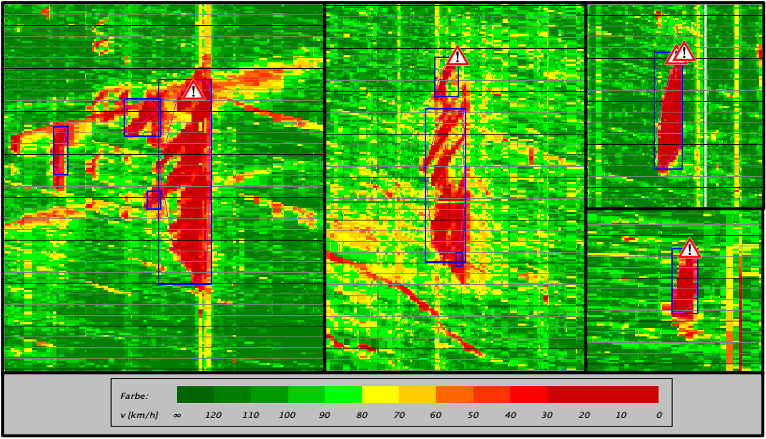
\includegraphics[scale=0.9]{images/cluster_final.png}
	\caption{Speed matrix plots of FCD data after clustering}
	\label{img:speedMatrixPlot_final_good}
\end{figure}

\section{Correlation Processing}
\label{analysis_processing_correlation}
The resulting datasets created by the evaluation tool (see section \cref{methodology_detection} \cref{methodology_matching} and \cref{methodology_data_processing}) which is tasked with the detection and clustering of jams and search for adjacent incidents, are then processed by the correlation tool (\cref{methodology_correlation_processing}). The correlation tool calculates multiple matrix tables with the correlation effect size, correlation significance and used correction coefficient for all variable combinations. From these tables and interpretation guidelines defined in \cref{correlation_coefficient_types} for each coefficient type, we can deviated the strength of correlation and significance (see \cref{correlation_significance}) for each variable combination. To recap \cref{correlation_coefficient_types}, \cref{tbl:correlation_interpretation_guidelines} shows the guidelines for a weak, moderate and strong correlation effect size of the coefficients $r$,$\eta$,$r_{pq}$,$\tau$ and $V$. The significance is evaluated by an $\alpha$-level of .05.
\begin{table}[ht!]
	\centering
	\begin{tabular}{r|c|c|c}  
		\toprule
		Coefficient & Weak 	& Moderate 	& Strong \\
		\midrule
		$r$ 		& .30	& .50		& .80 \\
		$\eta$ 		& < .06 & .06		& .14 \\
		$r_{pq}$	& < .30	& .30		& .50 \\
		$\tau$ 		& < .30	& .30		& .50 \\
		$V$ 		& < .30	& .30		& .40 \\
		\bottomrule
	\end{tabular}
	\caption{Correlation effect size interpretation for coefficient $r$,$\eta$,$r_{pq}$,$\tau$ and $V$}
	\label{tbl:correlation_interpretation_guidelines}
\end{table}
In the case of correlated and significant variables, it still needs to be determined what the found correlation predicates. This is done via the Post Hoc test, defined in \cref{correlation_posthoc}, which tests for for significance differences between the groups via the pairwise Wilcoxon $T$-test. The rest of this chapter is dedicated to elaborate on this tedious process of testing all groups for significance differences. This involves a enormous number of tables which need to be evaluated and involves repetitions, but is necessary to cover all assumptions and interpretations, referenced later on. For a summary of the significant differences and their interpretations, please forward to \cref{analysis_summary}.

% -------------------------
% -------- BAYSIS ---------
% -------------------------
% Global
% -----------------------------------
% -------- BAYSIS - Matched ---------
% -----------------------------------
\subsection{Congestion - Accidents in general}
\label{analysis_processing_correlation_baysis_matched}
The correlation matrix table for the complete congestion-accident matched dataset (see \cref{table:appendix_correlation_matrix_matched_cramers}) is visual presented in \cref{img:correlation_matrix_matched_cramers} showing the the correlation of each variable combination. When visual analyzing \cref{img:correlation_matrix_matched_cramers} and checking the guidelines for a strong correlation in reference to the applied coefficient (identifiable with \cref{table:appendix_coefficient_matrix_matched}) we get a list of strongly correlated variable combinations (see \cref{tbl:correlation_list_baysis_matched}). Since the focus of the thesis are the correlations between accidents and jams, these are only collected from the bottom-left corner of the matrix, where the congestion and accidents variables intersect. Correlations of the kind congestion - congestion or accident - accident are not considered.
\begin{table}[ht]
	\centering
	\begin{tabular}{c|l}  
		\toprule
		Category & Strong \\
		\midrule
		Str & TMax, TAvg, SMax, SAvg, TDist, SDist, Cov \\ 
 		Kat & TMax, TAvg, SAvg, TDist \\
 		Typ & TDist, Cov \\
 		%Betei & & \\
 		UArt1 & SAvg, TDist, Cov \\ % + SMax
 		%UArt2 & & \\
 		AUrs1 & SAvg, TDist, SDist, Cov, TLHGV \\ % + SMax
 		%AUrs2 & & \\
 		AufHi & TMax, TAvg, TDist, Cov \\
 		%Alkoh & & \\
 		%Char1 & & \\ -> Str ??
 		%Char2 & & \\
 		%Bes1 & & \\
 		Lich1 & Cov \\
 		Lich2 & Cov \\ % + Lich2
 		Zust1 & Cov \\ % -> Str ??
 		%Zust2 & & \\
 		%Fstf & & \\ % -> Str ??
 		WoTag & Cov \\
 		%FeiTag & & \\
		Month & Cov \\ % + TMax. SMAx
		\bottomrule
	\end{tabular}
	\caption{List of incident variables and their strong correlated congestion variable from the congestion-accident matched data}
	\label{tbl:correlation_list_baysis_matched}
\end{table}
Next we need to verify that the correlation is significant and what the correlation predicates. Therefore each correlation will be evaluated with the Post Hoc test, defined in \cref{correlation_posthoc}. In the following sections, the correlated relations of the variables in \cref{tbl:correlation_list_baysis_matched} are analyzed and an interpretation of each significant correlation is introduced. Groups with an insufficient sample size (see \cref{correlation_uncertainty}) are neglected and not shown. The descriptive tables, showing the count ($n$), mean ($\bar{x}$), standard deviation ($\sigma$), median ($\tilde{x}$), $min$, $max$ and range ($\Delta$) therefore only contain groups with significant sample sizes.
\begin{figure}[!ht]
	\centering
	\makebox[\textwidth][c]{%
		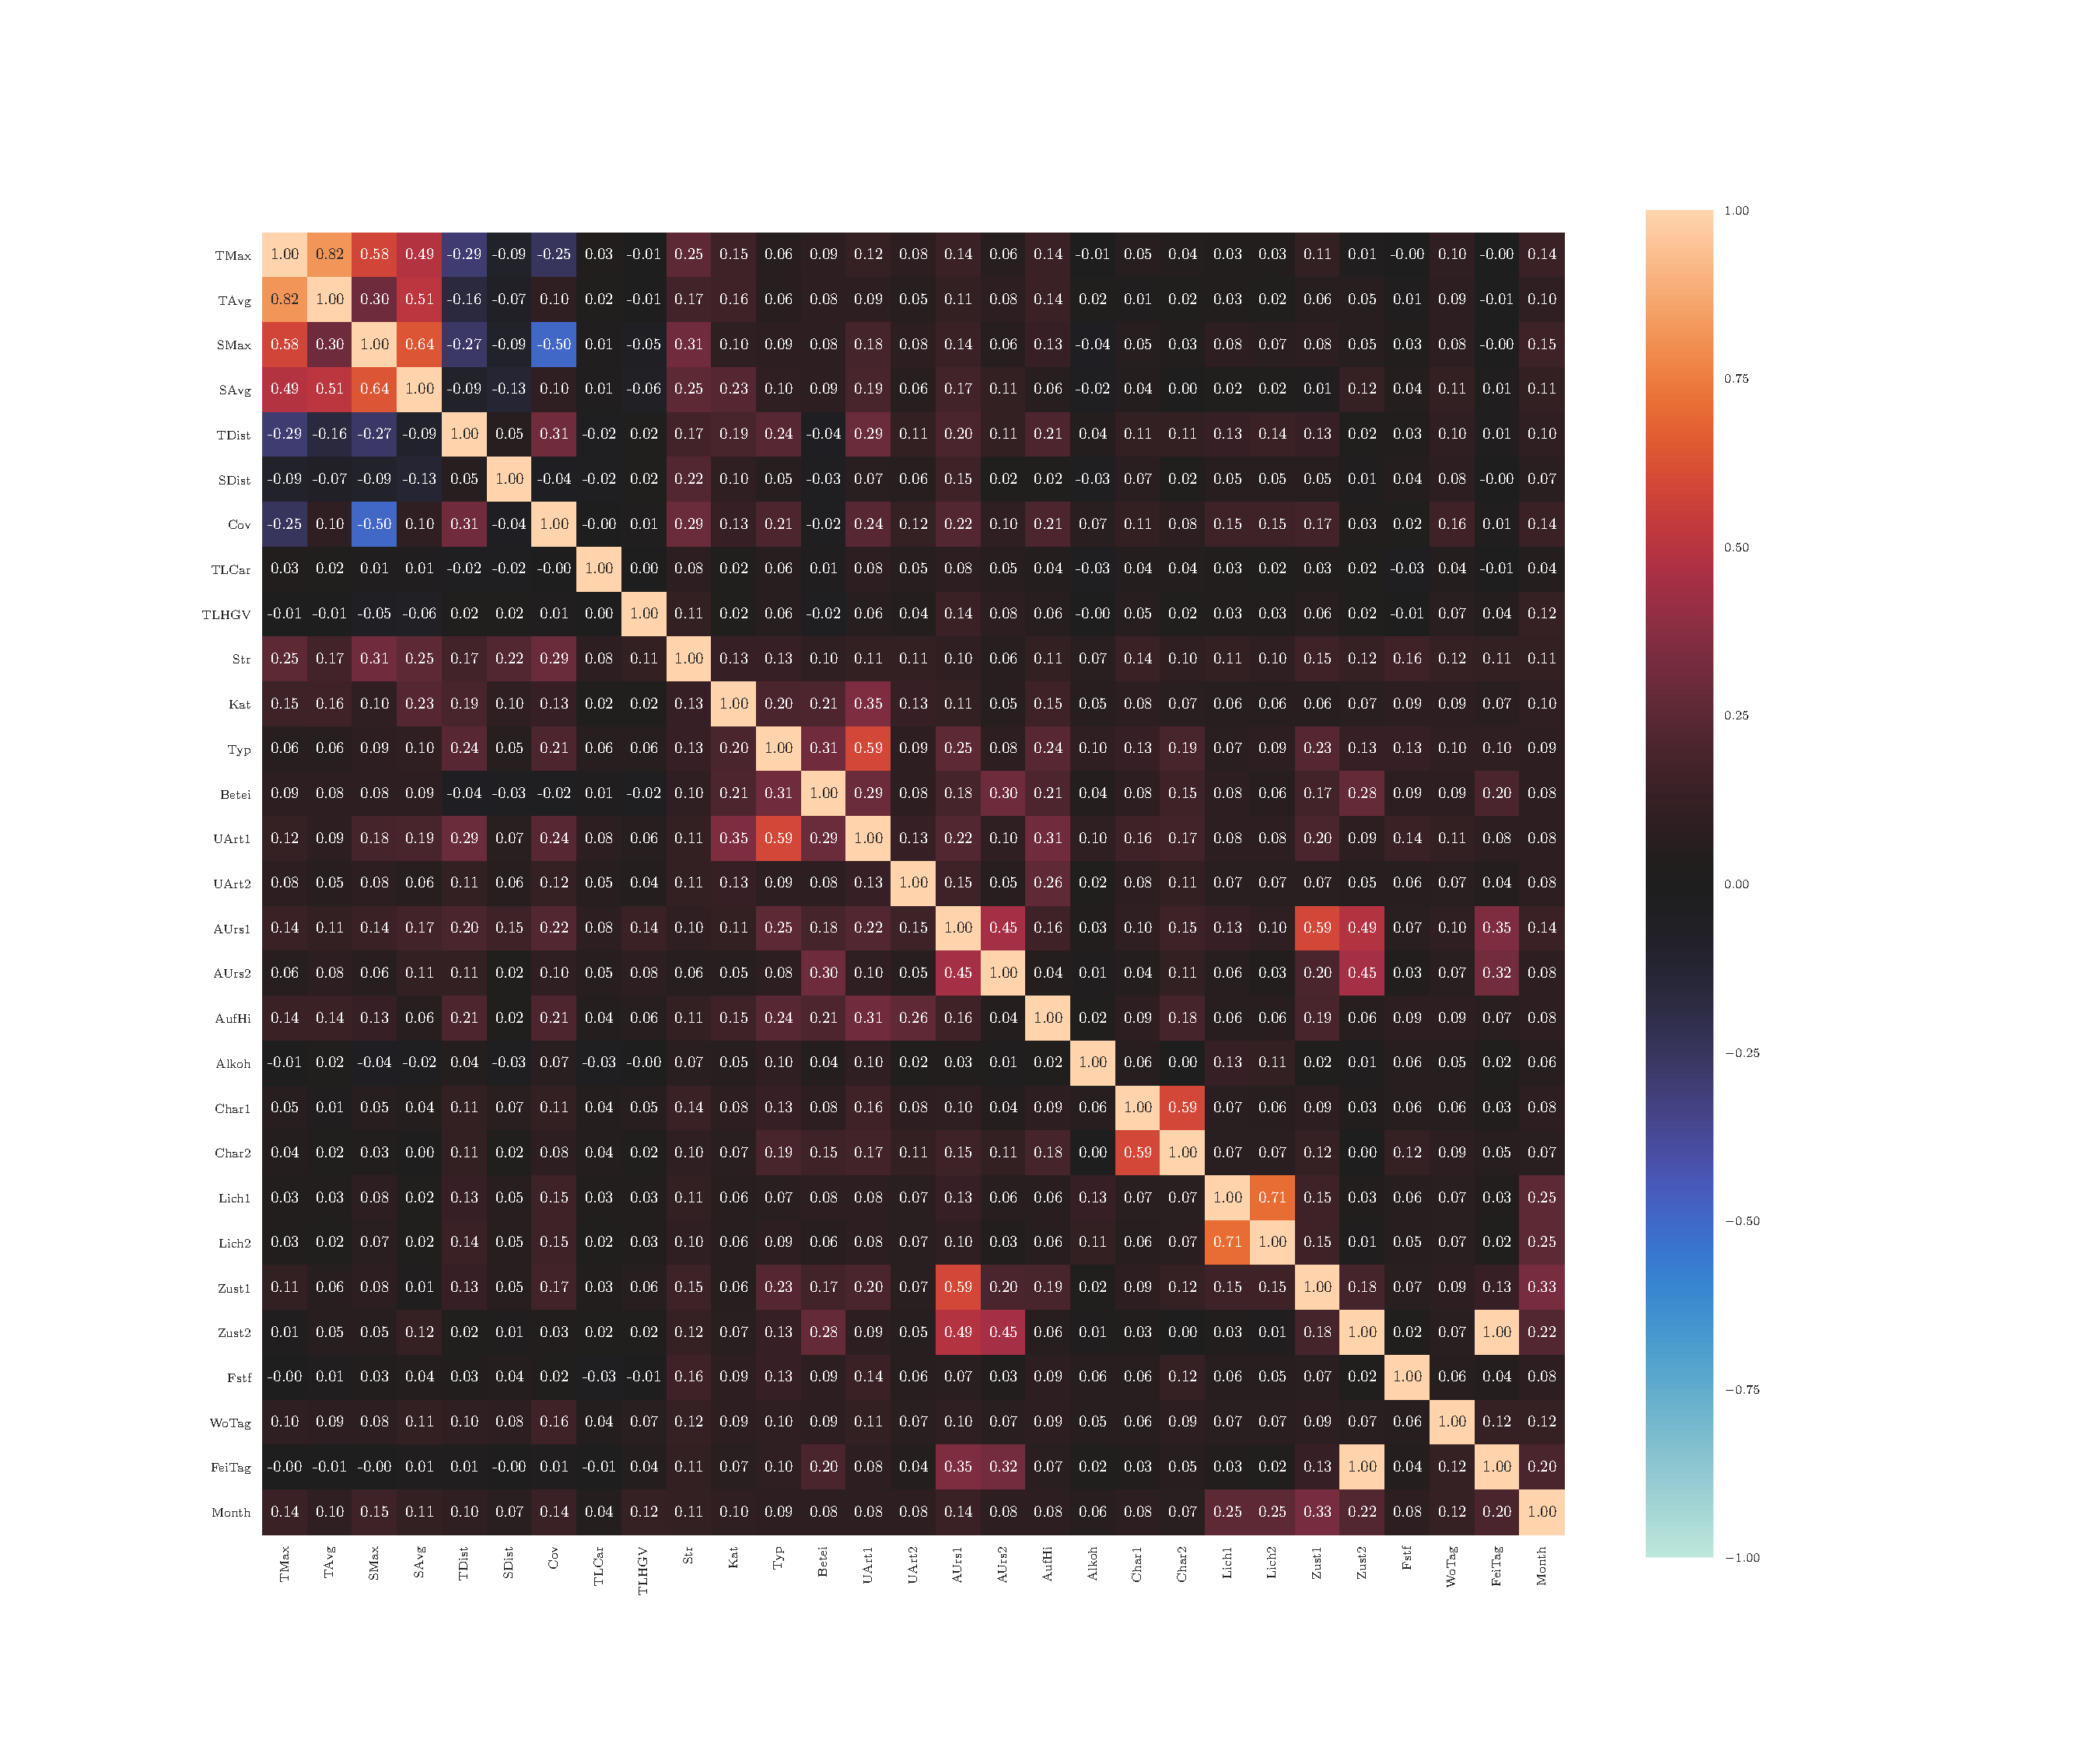
\includegraphics[width=1.4\textwidth, trim=0cm 2.5cm 6cm 3cm]{CorrAnalysis/data/BAYSIS/02_matched/plots/baysis_matched_corr_cramers}%
	}
	\caption{Correlation matrix for congestion-accident matched data calculated with $V$, $\eta$, $\tau$, $r_{pq}$, $r$}
	\label{img:correlation_matrix_matched_cramers}
\end{figure}

% --------------------------
% -------- Strasse ---------
% --------------------------
\centerheading{Street}
This section analyzes the correlated relations of the accident variable \textit{Str}. The correlations of \textit{Str} - \textit{TDist} and \textit{Str} - \textit{SDist} produces a $p$-value above the $\alpha$-level in the Kruskal-Wallis test. The null hypothesis therefore can't be rejected for these relations and there are no significant groups to identify.

The Kruskal-Wallis test of \textit{Str} - \textit{TMax} produces a $p$-value below 0.0001, which is below the $\alpha$-level. The null hypothesis can therefore be rejected, which means that there is a significant difference between the groups of \textit{Str}. To identify the significant groups the pairwise Wilcoxon $T$-test of \textit{Str}-\textit{TMax} produces \cref{tbl:wilcoxon_baysis_matched_Str_TMax}. 
\begin{table}[ht!]
	\tiny
	\setlength{\tabcolsep}{4pt}
	\centering
	\begin{tabular}{rrrrrrrrrrrrrrrrr}
		\toprule
				& A3 & A6 & A9 & A70 & A96 & A7 & A73 & A99 & A92 & A93 & A94 & A72 & A995 & A95 & A71 & A45 \\ 
		\midrule
		% A6 		& 0.00 &  &  &  &  &  &  &  &  &  &  &  &  &  &  &  \\ 
		A9 		& \red{0.01} & 1.00 &  &  &  &  &  &  &  &  &  &  &  &  &  &  \\ 
		A70 	& \red{0.03} & 1.00 & 1.00 &  &  &  &  &  &  &  &  &  &  &  &  &  \\ 
		A96 	& \red{0.00} & 1.00 & 0.27 & 1.00 &  &  &  &  &  &  &  &  &  &  &  &  \\ 
		A7 		& \red{0.00} & 1.00 & 1.00 & 1.00 & 1.00 &  &  &  &  &  &  &  &  &  &  &  \\ 
		A73 	& \red{0.00} & 1.00 & 0.31 & 1.00 & 1.00 & 1.00 &  &  &  &  &  &  &  &  &  &  \\ 
		% A99 	& 1.00 & 1.00 & 1.00 & 1.00 & 0.50 & 1.00 & 0.59 &  &  &  &  &  &  &  &  &  \\ 
		A92 	& \red{0.00} & 1.00 & 0.16 & 1.00 & 1.00 & 1.00 & 1.00 & 0.22 &  &  &  &  &  &  &  &  \\ 
		% A93 	& 1.00 & 1.00 & 1.00 & 1.00 & 1.00 & 1.00 & 1.00 & 1.00 & 1.00 &  &  &  &  &  &  &  \\ 
		A94 	& \red{0.01} & 1.00 & 1.00 & 1.00 & 1.00 & 1.00 & 1.00 & 1.00 & 1.00 & 1.00 &  &  &  &  &  &  \\ 
		% A72 	& 1.00 & 1.00 & 1.00 & 1.00 & 1.00 & 1.00 & 1.00 & 1.00 & 1.00 & 1.00 & 1.00 &  &  &  &  &  \\ 
		% A995 	& 1.00 & 1.00 & 1.00 & 1.00 & 1.00 & 1.00 & 1.00 & 1.00 & 1.00 & 1.00 & 1.00 & 1.00 &  &  &  &  \\ 
		% A95 	& 1.00 & 1.00 & 1.00 & 1.00 & 1.00 & 1.00 & 1.00 & 1.00 & 1.00 & 1.00 & 1.00 & 1.00 & 1.00 &  &  &  \\ 
		% A71 	& 1.00 & 1.00 & 1.00 & 1.00 & 1.00 & 1.00 & 1.00 & 1.00 & 1.00 & 1.00 & 1.00 & 1.00 & 1.00 & 1.00 &  &  \\ 
		% A45 	& 1.00 & 1.00 & 1.00 & 1.00 & 1.00 & 1.00 & 1.00 & 1.00 & 1.00 & 1.00 & 1.00 & 1.00 & 1.00 & 1.00 & 1.00 &  \\ 
		% A980 	& 1.00 & 1.00 & 1.00 & 1.00 & 1.00 & 1.00 & 1.00 & 1.00 & 1.00 & 1.00 & 1.00 & 1.00 & 1.00 & 1.00 & 1.00 & 1.00 \\ 
		\bottomrule
	\end{tabular}
	\caption{Pairwise Wilcoxon $T$-test for \textit{Street} and \textit{Maximal Temporal Extent}}
	\label{tbl:wilcoxon_baysis_matched_Str_TMax}
\end{table}
It shows that the groups A6, A9, A7, A70, A73, A92, A94 and A96 differ from group A3, but is no distinctive general trend.
\begin{table}[ht!]
	\tiny
	\centering
	\begin{tabular}{c|c|c|c|c|c|c|c}
		\toprule
		Group & $n$ & $\bar{x}$ & $\sigma$ & $\tilde{x}$ & $min$ & $max$ & $\Delta$ \\ 
		\midrule
		A3  & 559 & 225.76 & 210.36 & 156.00 & 9  & 1323 & 1314 \\ 
		A6  & 127 & 153.05 & 150.42 & 108.00 & 12 & 864  & 852  \\ 
		A9  & 466 & 170.85 & 151.33 & 118.50 & 9  & 1194 & 1185 \\ 
		A70 & 31  & 106.55 & 79.42  & 81.00  & 24 & 369  & 345  \\ 
		A96 & 155 & 118.32 & 81.05  & 108.00 & 12 & 384  & 372  \\ 
		A7  & 130 & 153.37 & 194.10 & 102.00 & 9  & 1341 & 1332 \\ 
		A73 & 129 & 125.95 & 135.01 & 93.00  & 12 & 1323 & 1311 \\ 
		A99 & 116 & 169.09 & 136.72 & 138.00 & 15 & 681  & 666  \\ 
		A92 & 66  & 103.86 & 65.69  & 87.00  & 18 & 354  & 336  \\ 
		A93 & 21  & 163.57 & 155.71 & 111.00 & 36 & 588  & 552  \\ 
		A94 & 37  & 101.59 & 54.60  & 99.00  & 15 & 249  & 234  \\ 
 		\bottomrule
	\end{tabular}
	\caption{Group descriptives of \textit{Street} and \textit{Maximal Temporal Extent}}
	\label{tbl:descriptives_baysis_matched_Str_TMax}
	%\vspace{-8mm}
\end{table}
The descriptives from \cref{tbl:descriptives_baysis_matched_Str_TMax} show that the mean value of A3 is 27\,\% - 57\,\% higher than the means of A6, A7, A9, A70, A73, A92, and A94. It can be interpreted that accidents on the A3 are associated with significantly longer (temporal) jams than on the A6, A9, A7, A70, A73, A92, and A94. The $\sigma$ supports this interpretation of by $\bar{x}$. The descriptives clearly show three ranked groups of short (A94, A93, A92, A70), medium (A99, A73, A7, A96, A9, A6) and long (A3).

The Kruskal-Wallis test of \textit{Str} - \textit{TAvg} produces a $p$-value of 0.0004, which is below the $\alpha$-level. The null hypothesis can therefore be rejected, which means there is a significant difference between the groups of \textit{Str}. To identify the significant groups the pairwise Wilcoxon $T$-test of \textit{Str}-\textit{TAvg} produces \cref{tbl:wilcoxon_baysis_matched_Str_TAvg}. 
\begin{table}[ht!]
	\tiny
	\setlength{\tabcolsep}{4pt}
	\centering
	\begin{tabular}{rrrrrrrrrrrrrrrrr}
		\toprule
				& A3 & A6 & A9 & A70 & A96 & A7 & A73 & A99 & A92 & A93 & A94 & A72 & A995 & A95 & A71 & A45 \\ 
		\midrule
		% A6 	 & 0.84 &  &  &  &  &  &  &  &  &  &  &  &  &  &  &  \\ 
		% A9 	 & 0.36 & 1.00 &  &  &  &  &  &  &  &  &  &  &  &  &  &  \\ 
		% A70	 & 1.00 & 1.00 & 1.00 &  &  &  &  &  &  &  &  &  &  &  &  &  \\ 
		% A96  & 0.10 & 1.00 & 1.00 & 1.00 &  &  &  &  &  &  &  &  &  &  &  &  \\ 
		% A7 	 & 1.00 & 1.00 & 1.00 & 1.00 & 1.00 &  &  &  &  &  &  &  &  &  &  &  \\ 
		A73  & \red{0.00} & 1.00 & 0.51 & 1.00 & 1.00 & 1.00 &  &  &  &  &  &  &  &  &  &  \\ 
		A99  & \red{0.02} & 1.00 & 1.00 & 1.00 & 1.00 & 1.00 & 1.00 &  &  &  &  &  &  &  &  &  \\ 
		% A92  & 0.26 & 1.00 & 1.00 & 1.00 & 1.00 & 1.00 & 1.00 & 1.00 &  &  &  &  &  &  &  &  \\ 
		% A93  & 1.00 & 1.00 & 1.00 & 1.00 & 1.00 & 1.00 & 1.00 & 1.00 & 1.00 &  &  &  &  &  &  &  \\ 
		% A94  & 0.28 & 1.00 & 1.00 & 1.00 & 1.00 & 1.00 & 1.00 & 1.00 & 1.00 & 1.00 &  &  &  &  &  &  \\ 
		% A72  & 1.00 & 1.00 & 1.00 & 1.00 & 1.00 & 1.00 & 1.00 & 1.00 & 1.00 & 1.00 & 1.00 &  &  &  &  &  \\ 
		% A995 & 1.00 & 1.00 & 1.00 & 1.00 & 1.00 & 1.00 & 1.00 & 1.00 & 1.00 & 1.00 & 1.00 & 1.00 &  &  &  &  \\ 
		% A95  & 1.00 & 1.00 & 1.00 & 1.00 & 1.00 & 1.00 & 1.00 & 1.00 & 1.00 & 1.00 & 1.00 & 1.00 & 1.00 &  &  &  \\ 
		% A71	 & 1.00 & 1.00 & 1.00 & 1.00 & 1.00 & 1.00 & 1.00 & 1.00 & 1.00 & 1.00 & 1.00 & 1.00 & 1.00 & 1.00 &  &  \\ 
		% A45  & 1.00 & 1.00 & 1.00 & 1.00 & 1.00 & 1.00 & 1.00 & 1.00 & 1.00 & 1.00 & 1.00 & 1.00 & 1.00 & 1.00 & 1.00 &  \\ 
		% A980 & 1.00 & 1.00 & 1.00 & 1.00 & 1.00 & 1.00 & 1.00 & 1.00 & 1.00 & 1.00 & 1.00 & 1.00 & 1.00 & 1.00 & 1.00 & 1.00 \\
		\bottomrule
	\end{tabular}
	\caption{Pairwise Wilcoxon $T$-test for \textit{Street} and \textit{Average Temporal Extent}}
	\label{tbl:wilcoxon_baysis_matched_Str_TAvg}
\end{table}
The table shows, that the groups A73 and A99 differ from group A3, but there is no distinctive general trend.
\begin{table}[ht!]
	\tiny
	\centering
	\begin{tabular}{c|c|c|c|c|c|c|c}
		\toprule
		Group & $n$ & $\bar{x}$ & $\sigma$ & $\tilde{x}$ & $min$ & $max$ & $\Delta$ \\  
		\midrule
		A3  & 559 & 89.66 & 98.94  & 65.00 & 4  & 1260 & 1256 \\ 
		A6  & 127 & 69.94 & 65.86  & 56.00 & 3  & 376  & 373  \\ 
		A9  & 466 & 72.92 & 64.55  & 54.00 & 4  & 575  & 571  \\ 
		A70 & 31  & 50.10 & 23.99  & 49.00 & 10 & 99   & 89   \\ 
		A96 & 155 & 61.37 & 44.31  & 52.50 & 5  & 247  & 242  \\ 
		A7  & 130 & 86.55 & 146.82 & 59.50 & 6  & 1326 & 1320 \\ 
		A73 & 129 & 54.78 & 42.48  & 45.00 & 6  & 274  & 268  \\ 
		A99 & 116 & 58.97 & 48.35  & 47.50 & 4  & 295  & 291  \\ 
		A92 & 66  & 55.24 & 36.43  & 51.50 & 8  & 235  & 227  \\ 
		A93 & 21  & 82.33 & 91.10  & 48.00 & 7  & 343  & 336  \\ 
		A94 & 37  & 49.86 & 31.63  & 44.00 & 14 & 145  & 131  \\ 
		\bottomrule
	\end{tabular}
	\caption{Group descriptives for \textit{Street} and \textit{Average Temporal Extent}}
	\label{tbl:descriptives_baysis_matched_Str_TAvg}
	%\vspace{-8mm}
\end{table}
The descriptives from \cref{tbl:descriptives_baysis_matched_Str_TAvg} show that the mean value of A3 is about $\frac{1}{3}$ higher than the means of A73 and A96. We can interpret that accidents on the A3 are associated with significantly longer (temporal) jams than on A73 and A96. The descriptives also show general increase of $\bar{x}$ and $\sigma$ around 35\,\% between the roads A94, A92, A73 and A70 to A3, A6, A7 and A9.

The Kruskal-Wallis test of \textit{Str} - \textit{SMax} produces a $p$-value below 0.0001, which is below the $\alpha$-level. The null hypothesis can therefore be rejected, which means there is a significant difference between the groups of \textit{Str}. To identify the significant groups, a pairwise Wilcoxon $T$-test for \textit{Str} - \textit{SMax} is run, which produces \cref{tbl:wilcoxon_baysis_matched_Str_SMax}.
\begin{table}[ht!]
	\tiny
	\setlength{\tabcolsep}{4pt}
	\centering
	\begin{tabular}{rrrrrrrrrrrrrrrrr}
		\toprule
				& A3   & A6   & A9   & A70  & A96  & A7   & A73   & A99 & A92 & A93 & A94 & A72 & A995 & A95 & A71 & A45 \\ 
		\midrule
		% A6 		& 0.40 &  &  &  &  &  &  &  &  &  &  &  &  &  &  &  \\ 
		A9 		& \red{0.00} & 1.00 &  &  &  &  &  &  &  &  &  &  &  &  &  &  \\ 
		A70 	& \red{0.00} & 0.83 & 0.54 &  &  &  &  &  &  &  &  &  &  &  &  &  \\ 
		A96 	& \red{0.00} & 1.00 & 0.14 & 1.00 &  &  &  &  &  &  &  &  &  &  &  &  \\ 
		A7 		& \red{0.00} & 1.00 & 1.00 & 1.00 & 1.00 &  &  &  &  &  &  &  &  &  &  &  \\ 
		A73 	& \red{0.00} & \red{0.00} & \red{0.00} & 1.00 & 1.00 & 0.59 &  &  &  &  &  &  &  &  &  &  \\ 
		A99 	& 1.00 & 1.00 & 1.00 & 0.80 & 0.31 & 1.00 & \red{0.00} &  &  &  &  &  &  &  &  &  \\ 
		A92 	& \red{0.00} & \red{0.00} & \red{0.00} & 1.00 & 1.00 & 1.00 & 1.00 & \red{0.00} &  &  &  &  &  &  &  &  \\ 
		A93 	& \red{0.03} & 1.00 & 1.00 & 1.00 & 1.00 & 1.00 & 1.00 & 1.00 & 1.00 &  &  &  &  &  &  &  \\ 
		A94 	& \red{0.00} & 0.11 & \red{0.03} & 1.00 & 1.00 & 1.00 & 1.00 & 0.09 & 1.00 & 1.00 &  &  &  &  &  &  \\ 
		% A72 	& 1.00 & 1.00 & 1.00 & 1.00 & 1.00 & 1.00 & 1.00 & 1.00 & 1.00 & 1.00 & 1.00 &  &  &  &  &  \\ 
		% A995 	& 1.00 & 1.00 & 1.00 & 1.00 & 1.00 & 1.00 & 1.00 & 1.00 & 1.00 & 1.00 & 1.00 & 1.00 &  &  &  &  \\ 
		% A95 	& 1.00 & 1.00 & 1.00 & 1.00 & 1.00 & 1.00 & 1.00 & 1.00 & 1.00 & 1.00 & 1.00 & 1.00 & 1.00 &  &  &  \\ 
		% A71 	& 1.00 & 1.00 & 1.00 & 1.00 & 1.00 & 1.00 & 1.00 & 1.00 & 1.00 & 1.00 & 1.00 & 1.00 & 1.00 & 1.00 &  &  \\ 
		% A45 	& 1.00 & 1.00 & 1.00 & 1.00 & 1.00 & 1.00 & 1.00 & 1.00 & 1.00 & 1.00 & 1.00 & 1.00 & 1.00 & 1.00 & 1.00 &  \\ 
		% A980 	& 1.00 & 1.00 & 1.00 & 1.00 & 1.00 & 1.00 & 1.00 & 1.00 & 1.00 & 1.00 & 1.00 & 1.00 & 1.00 & 1.00 & 1.00 & 1.00 \\ 
		\bottomrule
	\end{tabular}
	\caption{Pairwise Wilcoxon $T$-test for \textit{Street} and \textit{Maximal Spatial Extent}}
	\label{tbl:wilcoxon_baysis_matched_Str_SMax}
\end{table}
\cref{tbl:wilcoxon_baysis_matched_Str_SMax} shows, that the groups A7, A9, A70, A73, A92, A94 and A96 differ from group A3. The groups A73 and A92 further differ from group A6 and A9. The group A99 differs from group A73 and group A92 differs from A99, but there is no distinctive general trend.
\begin{table}[ht!]
	\tiny
	\centering
	\begin{tabular}{c|c|c|c|c|c|c|c}
		\toprule
		Group & $n$ & $\bar{x}$ & $\sigma$ & $\tilde{x}$ & $min$ & $max$ & $\Delta$ \\  
		\midrule
		A3  & 559 & 13874.96 & 10064.51 & 11014.00 & 1084 & 46328 & 45244 \\ 
		A6  & 127 & 11067.98 & 8428.07  & 8634.00  & 965  & 43156 & 42191 \\ 
		A9  & 466 & 10680.48 & 7724.45  & 8977.50  & 832  & 49765 & 48933 \\ 
		A70 & 31  & 6676.39  & 3640.24  & 6136.00  & 1841 & 13058 & 11217 \\ 
		A96 & 155 & 8551.75  & 6431.18  & 6238.00  & 971  & 27965 & 26994 \\ 
		A7  & 130 & 9018.27  & 7293.14  & 7051.50  & 1108 & 43244 & 42136 \\ 
		A73 & 129 & 6502.88  & 5033.20  & 5327.00  & 1036 & 33764 & 32728 \\ 
		A99 & 116 & 13244.02 & 11313.27 & 9439.50  & 1280 & 48278 & 46998 \\ 
		A92 & 66  & 6186.80  & 4000.10  & 4936.50  & 1176 & 23291 & 22115 \\ 
		A93 & 21  & 6765.00  & 4403.32  & 5323.00  & 1244 & 16922 & 15678 \\ 
		A94 & 37  & 6220.38  & 3984.46  & 5768.00  & 1167 & 15550 & 14383 \\ 
		\bottomrule
	\end{tabular}
	\caption{Group descriptives of \textit{Street} and \textit{Maximal Spatial Extent}}
	\label{tbl:descriptives_baysis_matched_Str_SMax}
	%\vspace{-8mm}
\end{table}
The descriptives from \cref{tbl:descriptives_baysis_matched_Str_SMax} show that the mean of A3 is 44\,\% - 66\,\% higher than the means of A7, A9, A70, A73, A92, A94 and A96. It also shows that the groups A6, A9 and A99 have a up to 50\,\% higher mean than the groups A73 and A92. We can interpret that accidents on the A3, A6, A9 and A99 are associated with significantly longer (spatial) jams than on A7, A73, A92, A94 and A96. Based on the $\bar{x}$ and $\sigma$ the roads can be separated into three groups of short (A94, A93, A92, A73 and A70), medium (A96 and A7) and long (A3, A6, A9 and A99).

The Kruskal-Wallis test of \textit{Str} - \textit{SAvg} produces a $p$-value of 0.0027, which is below $\alpha=.05$. The null hypothesis can therefore be rejected, which means there is a significant difference between the groups of \textit{Str}. To identify the significant groups, a pairwise Wilcoxon $T$-test for \textit{Str} - \textit{SAvg} is run, which produces \cref{tbl:wilcoxon_baysis_matched_Str_SAvg}.
\begin{table}[ht!]
	\tiny
	\setlength{\tabcolsep}{4pt}
	\centering
	\begin{tabular}{rrrrrrrrrrrrrrrrr}
		\toprule
	 		 & A3 & A6 & A9 & A70 & A96 & A7 & A73 & A99 & A92 & A93 & A94 & A72 & A995 & A95 & A71 & A45 \\ 
		\midrule
		% A6   & 1.00 &  &  &  &  &  &  &  &  &  &  &  &  &  &  &  \\ 
	  	% A9   & 1.00 & 1.00 &  &  &  &  &  &  &  &  &  &  &  &  &  &  \\ 
	  	A70  & \red{0.05} & 0.83 & 0.71 &  &  &  &  &  &  &  &  &  &  &  &  &  \\ 
	  	A96  & \red{0.05} & 1.00 & 1.00 & 1.00 &  &  &  &  &  &  &  &  &  &  &  &  \\ 
	  	% A7   & 1.00 & 1.00 & 1.00 & 1.00 & 1.00 &  &  &  &  &  &  &  &  &  &  &  \\ 
	  	A73  & \red{0.00} & \red{0.00} & \red{0.00} & 1.00 & \red{0.00} & \red{0.00} &  &  &  &  &  &  &  &  &  &  \\ 
	  	A99  & \red{0.00} & 1.00 & 0.06 & 1.00 & 1.00 & 1.00 & 0.51 &  &  &  &  &  &  &  &  &  \\ 
	  	A92  & \red{0.00} & 0.61 & \red{0.03} & 1.00 & 1.00 & 1.00 & 1.00 & 1.00 &  &  &  &  &  &  &  &  \\ 
	  	A93  & \red{0.03} & 0.46 & 0.16 & 1.00 & 1.00 & 1.00 & 1.00 & 1.00 & 1.00 &  &  &  &  &  &  &  \\ 
	  	A94  & \red{0.00} & 0.07 & 0.01 & 1.00 & 0.36 & 0.31 & 1.00 & 1.00 & 1.00 & 1.00 &  &  &  &  &  &  \\ 
	  	% A72  & 1.00 & 1.00 & 1.00 & 1.00 & 1.00 & 1.00 & 1.00 & 1.00 & 1.00 & 1.00 & 1.00 &  &  &  &  &  \\ 
	  	% A995 & 1.00 & 1.00 & 1.00 & 1.00 & 1.00 & 1.00 & 1.00 & 1.00 & 1.00 & 1.00 & 1.00 & 1.00 &  &  &  &  \\ 
	  	% A95  & 1.00 & 1.00 & 1.00 & 1.00 & 1.00 & 1.00 & 1.00 & 1.00 & 1.00 & 1.00 & 1.00 & 1.00 & 1.00 &  &  &  \\ 
	  	% A71  & 1.00 & 1.00 & 1.00 & 1.00 & 1.00 & 1.00 & 1.00 & 1.00 & 1.00 & 1.00 & 1.00 & 1.00 & 1.00 & 1.00 &  &  \\ 
	  	% A45  & 1.00 & 1.00 & 1.00 & 1.00 & 1.00 & 1.00 & 1.00 & 1.00 & 1.00 & 1.00 & 1.00 & 1.00 & 1.00 & 1.00 & 1.00 &  \\ 
	  	% A980 & 1.00 & 1.00 & 1.00 & 1.00 & 1.00 & 1.00 & 1.00 & 1.00 & 1.00 & 1.00 & 1.00 & 1.00 & 1.00 & 1.00 & 1.00 & 1.00 \\ 
		\bottomrule
	\end{tabular}
	\caption{Pairwise Wilcoxon $T$-test for \textit{Street} and \textit{Average Spatial Extent}}
	\label{tbl:wilcoxon_baysis_matched_Str_SAvg}
\end{table}
\cref{tbl:wilcoxon_baysis_matched_Str_SAvg} shows, that the groups A70, A73, A92, A93, A94, A96 and A99 differ from group A3. The groups A73, A94 further differ from group A6 as well as A73, A99, A92 and A94 from group A9, but there is no distinctive general trend.
\begin{table}[ht!]
	\tiny
	\centering
	\begin{tabular}{c|c|c|c|c|c|c|c}
	  	\toprule
	 	Group & $n$ & $\bar{x}$ & $\sigma$ & $\tilde{x}$ & $min$ & $max$ & $\Delta$ \\  
	  	\midrule
		A3  & 559 & 4537.56 & 2735.62 & 3986.00 & 135  & 17805 & 17670 \\ 
	  	A6  & 127 & 4361.50 & 3042.71 & 3235.00 & 458  & 16851 & 16393 \\ 
	  	A9  & 466 & 4187.15 & 2569.83 & 3700.50 & 393  & 15132 & 14739 \\ 
	  	A70 & 31  & 3010.45 & 2067.63 & 1974.00 & 1008 & 9937  & 8929 \\ 
	  	A96 & 155 & 3678.39 & 2172.99 & 3299.00 & 387  & 10182 & 9795 \\ 
	  	A7  & 130 & 4141.68 & 3026.58 & 3537.50 & 643  & 16571 & 15928 \\ 
	  	A73 & 129 & 2683.97 & 1981.91 & 2232.00 & 544  & 11832 & 11288 \\ 
	  	A99 & 116 & 3240.97 & 1878.87 & 2978.00 & 583  & 8426  & 7843 \\ 
	  	A92 & 66  & 2926.15 & 1521.59 & 2931.50 & 455  & 8970  & 8515 \\ 
	  	A93 & 21  & 2525.43 & 1443.21 & 2338.00 & 664  & 6779  & 6115 \\ 
	  	A94 & 37  & 2691.68 & 2023.38 & 2307.00 & 358  & 10393 & 10035 \\ 
	   	\bottomrule
	\end{tabular}
	\caption{Group descriptives of \textit{Street} and \textit{Average Spatial Extent}}
	\label{tbl:descriptives_baysis_matched_Str_SAvg}
	%\vspace{-8mm}
\end{table}
The descriptives from \cref{tbl:descriptives_baysis_matched_Str_SAvg} show that the mean of A3 is 45\,\% - 55\,\% higher the means of A70, A73, A92, A93, A94, A96 and A99. It also shows that the means of the groups A6, A9 and A99 is about 30\,\% higher mean than the groups A73 and A94. We can interpret that accidents on the A3, A6, A9 and A99 lead are associated with significantly longer (spatial) jams than on A70, A73, A92, A93, A94, A96 and A99. The groups can be separated into two groups based on $\bar{x}$ and $\sigma$. A3, A6, A9 and A7 tend to have longer (spatial) longer jams when A70, A96, A73, A99, A92, A93 and A94 tend to have shorter (spatial) jams.

The Kruskal-Wallis test of \textit{Str} - \textit{Cov} produces a $p$-value of 0.0018, which is below the $\alpha$-level. The null hypothesis can therefore be rejected, which means there is a significant difference between the groups of \textit{Str}. To identify the significant groups, a pairwise Wilcoxon $T$-test for \textit{Str} - \textit{Cov} is run, which produces \cref{tbl:wilcoxon_baysis_matched_Str_Cov}. 
\begin{table}[ht!]
	\tiny
	\setlength{\tabcolsep}{4pt}
	\centering
	\begin{tabular}{rrrrrrrrrrrrrrrrr}
	  	\toprule
				& A3   & A6   & A9   & A70  & A96  & A7   & A73 & A99 & A92 & A93 & A94 & A72 & A995 & A95 & A71 & A45 \\ 
	  	\midrule
		A6 		& \red{0.05} &  &  &  &  &  &  &  &  &  &  &  &  &  &  &  \\ 
	  	A9 		& \red{0.00} & 1.00 &  &  &  &  &  &  &  &  &  &  &  &  &  &  \\ 
	  	% A70 	& 1.00 & 1.00 & 1.00 &  &  &  &  &  &  &  &  &  &  &  &  &  \\ 
	  	A96 	& \red{0.00} & 1.00 & \red{0.00} & 1.00 &  &  &  &  &  &  &  &  &  &  &  &  \\ 
	  	A7 		& \red{0.00} & 1.00 & \red{0.01} & 1.00 & 1.00 &  &  &  &  &  &  &  &  &  &  &  \\ 
	  	A73 	& \red{0.04} & 1.00 & 1.00 & 1.00 & 1.00 & 1.00 &  &  &  &  &  &  &  &  &  &  \\ 
	  	A99 	& 0.88 & \red{0.00} & \red{0.00} & 0.09 & \red{0.00} & \red{0.00} & \red{0.00} &  &  &  &  &  &  &  &  &  \\ 
	  	A92 	& \red{0.00} & 1.00 & 0.12 & 1.00 & 1.00 & 1.00 & 1.00 & \red{0.00} &  &  &  &  &  &  &  &  \\ 
	  	% A93 	& 1.00 & 1.00 & 1.00 & 1.00 & 1.00 & 1.00 & 1.00 & 1.00 & 1.00 &  &  &  &  &  &  &  \\ 
	  	% A94 	& 1.00 & 1.00 & 1.00 & 1.00 & 1.00 & 1.00 & 1.00 & 0.13 & 1.00 & 1.00 &  &  &  &  &  &  \\ 
	  	% A72 	& 1.00 & 1.00 & 1.00 & 1.00 & 1.00 & 1.00 & 1.00 & 1.00 & 1.00 & 1.00 & 1.00 &  &  &  &  &  \\ 
	  	% A995 	& 1.00 & 1.00 & 1.00 & 1.00 & 1.00 & 1.00 & 1.00 & 1.00 & 1.00 & 1.00 & 1.00 & 1.00 &  &  &  &  \\ 
	  	% A95 	& 1.00 & 1.00 & 1.00 & 1.00 & 1.00 & 1.00 & 1.00 & 1.00 & 1.00 & 1.00 & 1.00 & 1.00 & 1.00 &  &  &  \\ 
	  	% A71 	& 1.00 & 1.00 & 1.00 & 1.00 & 1.00 & 1.00 & 1.00 & 1.00 & 1.00 & 1.00 & 1.00 & 1.00 & 1.00 & 1.00 &  &  \\ 
	  	% A45 	& 1.00 & 1.00 & 1.00 & 1.00 & 1.00 & 1.00 & 1.00 & 1.00 & 1.00 & 1.00 & 1.00 & 1.00 & 1.00 & 1.00 & 1.00 &  \\ 
	  	% A980 	& 1.00 & 1.00 & 1.00 & 1.00 & 1.00 & 1.00 & 1.00 & 1.00 & 1.00 & 1.00 & 1.00 & 1.00 & 1.00 & 1.00 & 1.00 & 1.00 \\ 
	   	\bottomrule
	\end{tabular}
	\caption{Pairwise Wilcoxon $T$-test for \textit{Street} and \textit{Coverage}}
	\label{tbl:wilcoxon_baysis_matched_Str_Cov}
\end{table}
\cref{tbl:wilcoxon_baysis_matched_Str_SAvg} shows, that the groups A6, A7, A9, A73, A92 and A96 differ from group A3. The group A99 differs from group A6 and groups A96, AA7, A99, A92 differ from group A9. The group A99 also differs from the groups A70, A96, A7 and A73, but there is no distinctive general trend. 
\begin{table}[ht!]
	\tiny
	\centering
	\begin{tabular}{c|c|c|c|c|c|c|c}
	  	\toprule
	 	Group & $n$ & $\bar{x}$ & $\sigma$ & $\tilde{x}$ & $min$ & $max$ & $\Delta$ \\   
	  	\midrule
		A3  & 559 & 38.44 & 19.04 & 36.00 & 2  & 100 & 98 \\ 
	  	A6  & 127 & 46.99 & 24.06 & 44.00 & 9  & 100 & 91 \\ 
	  	A9  & 466 & 43.93 & 18.49 & 41.00 & 6  & 100 & 94 \\ 
	  	A70 & 31  & 50.29 & 25.00 & 44.00 & 9  & 92  & 83 \\ 
	  	A96 & 155 & 51.94 & 21.38 & 54.00 & 2  & 100 & 98 \\ 
	  	A7  & 130 & 53.46 & 24.19 & 54.00 & 6  & 100 & 94 \\ 
	  	A73 & 129 & 46.49 & 22.88 & 42.00 & 7  & 100 & 93 \\ 
	  	A99 & 116 & 33.21 & 18.03 & 31.00 & 5  & 85  & 80 \\ 
	  	A92 & 66  & 53.15 & 21.80 & 52.50 & 14 & 98  & 84 \\ 
	  	A93 & 21  & 40.81 & 17.72 & 37.00 & 13 & 70  & 57 \\ 
	  	A94 & 37  & 47.76 & 23.69 & 44.00 & 11 & 88  & 77 \\ 	
	  	\bottomrule
	\end{tabular}
	\caption{Group descriptives of \textit{Street} and \textit{Coverage}}
	\label{tbl:descriptives_baysis_matched_Str_Cov}
	%\vspace{-8mm}
\end{table}
The descriptives from \cref{tbl:descriptives_baysis_matched_Str_Cov} show that the mean of A3 is 20\,\% - 30\,\% lower than the means of A6, A7, A9, A73, A92 and A96. It also shows that the mean of A6 is about $\frac{1}{3}$ higher than the mean of A99. We can interpret that accidents on the A3, A99 are associated with significantly less denser jams than on A6, A7, A9, A73, A70, A92 and A96.

% ----------------------
% -------- Kat ---------
% ----------------------
\centerheading{Kat}
\label{ana:baysis_global_Kat}
This section analyzes the correlated relations of the accident variable \textit{Kat}. The encoding and description of the variable \textit{Typ} is shown in \cref{tbl:baysis_dataset_Typ}. The Kruskal-Wallis rank sum test of \textit{Kat}-\textit{SAvg} produces a $p$-value above $\alpha$. The null hypothesis can't be rejected and there is no significant difference between the groups of \textit{Kat} in this relation.

The Kruskal-Wallis test of \textit{Kat}-\textit{TMax} produces a $p$-value of 0.0068, which is below $\alpha=.05$. The null hypothesis can therefore be rejected, which means there is a significant difference between the groups of \textit{Kat}. To identify the significant groups, a pairwise Wilcoxon $T$-test for \textit{Kat}-\textit{TMax} is run, which produces \cref{tbl:wilcoxon_baysis_matched_Kat_TMax}.
\begin{table}[ht]
	\tiny
	\centering
	\begin{tabular}{rrrr}
	  	\toprule
	 	& 1 & 2 & 3 \\ 
	  	\midrule
		2 & \red{0.00} &  &  \\ 
	  	3 & \red{0.00} & \red{0.01} &  \\ 
	  	7 & \red{0.00} & \red{0.02} & 0.78 \\ 
	   	\bottomrule
	\end{tabular}
	\caption{Pairwise Wilcoxon $T$-test for \textit{Kat} and \textit{Maximal Temporal Extent}}
	\label{tbl:wilcoxon_baysis_matched_Kat_TMax}
\end{table}
\cref{tbl:wilcoxon_baysis_matched_Kat_TMax} shows that all groups, besides of group 7 to group 3, have significant differences. 
\begin{table}[ht]
	\tiny
	\centering
	\begin{tabular}{c|c|c|c|c|c|c|c}
		\toprule
		Group & $n$ & $\bar{x}$ & $\sigma$ & $\tilde{x}$ & $min$ & $max$ & $\Delta$ \\   
	  	\midrule
		1 & 36  & 317.67 & 215.10 & 279 & 27 & 987  & 960 \\ 
	  	2 & 216 & 189.03 & 164.93 & 135 & 9  & 1257 & 1248 \\ 
	  	3 & 881 & 155.26 & 141.87 & 111 & 9  & 1323 & 1314 \\ 
	  	7 & 718 & 179.35 & 192.33 & 117 & 9  & 1341 & 1332 \\ 
	   	\bottomrule
	\end{tabular}
	\caption{Group descriptives of \textit{Kat} and \textit{Maximal Temporal Extent}}
	\label{tbl:descriptives_baysis_matched_Kat_TMax}
	%\vspace{-8mm}
\end{table}
% 189+155+179 / 3 = 174
% diff 317,174 = 143
% mean diff 189,155,179 = 29
The descriptives from \cref{tbl:descriptives_baysis_matched_Kat_TMax} present increasing means from lightly injured to deathly accident. We can interpret that the maximal temporal jam length  increases with the gravity of the accident. Also the difference of group 1 to group 2, 3 and 7 is quite substantial, which means that the accidents with deaths are associated with 143\,min longer jams, than others. The group of accidents with property damage does significantly differ from the others, but does not fit into the trend. A comparisons of means puts the property damage group in-between of accidents with slightly and heavily injured. The groups 2, 3 and 7 differ by 29\,min on average.

The Kruskal-Wallis test of \textit{Kat}-\textit{TAvg} produces a $p$-value of 0.0005, which is below $\alpha$. The null hypothesis can therefore be rejected, which means there is a significant difference between the groups of \textit{Kat}. To identify the significant groups, a pairwise Wilcoxon $T$-test for \textit{Kat}-\textit{TAvg} is run, which produces \cref{tbl:wilcoxon_baysis_matched_Kat_TAvg}.
\begin{table}[ht]
	\tiny
	\centering
	\begin{tabular}{rrrr}
	  	\toprule
	 	& 1 & 2 & 3 \\ 
	  	\midrule
		2 & \red{0.00} &  &  \\ 
	  	3 & \red{0.00} & \red{0.00} &  \\ 
	  	7 & \red{0.00} & \red{0.00} & \red{0.05} \\ 
	   	\bottomrule
	\end{tabular}
	\caption{Pairwise Wilcoxon $T$-test for \textit{Kat} and \textit{Average Temporal Extent}}
	\label{tbl:wilcoxon_baysis_matched_Kat_TAvg}
\end{table}
\cref{tbl:wilcoxon_baysis_matched_Kat_TAvg} shows that all groups have significant differences. The descriptives from \cref{tbl:descriptives_baysis_matched_Kat_TAvg} present increasing means from group 3 to 1.
\begin{table}[ht]
	\tiny
	\centering
	\begin{tabular}{c|c|c|c|c|c|c|c}
	  	\toprule
		Group & $n$ & $\bar{x}$ & $\sigma$ & $\tilde{x}$ & $min$ & $max$ & $\Delta$ \\ 
	  	\midrule
		1 & 36  & 156.06 & 104.55 & 143.00 & 20 & 502  & 482  \\ 
	  	2 & 216 & 88.31  & 79.73  & 66.50  & 7  & 703  & 696  \\ 
	  	3 & 881 & 67.32  & 53.98  & 54.00  & 3  & 469  & 466  \\ 
	  	7 & 718 & 74.08  & 103.32 & 51.00  & 4  & 1326 & 1322 \\ 
	   	\bottomrule
	\end{tabular}
	\caption{Group descriptives of \textit{Kat} and \textit{Average Temporal Extent}}
	\label{tbl:descriptives_baysis_matched_Kat_TAvg}
	%\vspace{-8mm}
\end{table}
% 88+67+74 / 3 = 76
% diff 156,76 = 80
% mean diff 88,67,74 = 10
We can interpret that the average temporal jam length increases with the gravity of the accident. Also the difference of group 1 to group 2, 3 and 7 is quite substantial, which means that the accidents with deaths are associated with 80\,min longer jams than others. The group of accidents with property damage does significantly differ from the others, but does not fit into the trend. A comparisons of means puts the group in-between of accidents with slightly and heavily injured. The groups 2, 3 and 7 differ by 10\,min on average. 

The Kruskal-Wallis test of \textit{Kat}-\textit{TDist} produces a $p$-value below 0.0001, which is way below the $\alpha$-level. The null hypothesis can therefore be rejected, which means there is a significant difference between the groups of \textit{Kat}. To identify the significant groups, a pairwise Wilcoxon $T$-test for \textit{Kat}-\textit{TDist} is run, which produces \cref{tbl:wilcoxon_baysis_matched_Kat_TDist}. 
\begin{table}[ht]
	\tiny
	\centering
	\begin{tabular}{rrrr}
		\toprule
		& 1 & 2 & 3 \\ 
		\midrule
		2 & \red{0.05} &  &  \\ 
		3 & \red{0.00} & \red{0.00} &  \\ 
		7 & \red{0.00} & \red{0.00} & \red{0.00} \\ 
		\bottomrule
	\end{tabular}
	\caption{Pairwise Wilcoxon $T$-test for \textit{Kat} and \textit{Temporal Distance}}
	\label{tbl:wilcoxon_baysis_matched_Kat_TDist}
\end{table}
\cref{tbl:wilcoxon_baysis_matched_Kat_TDist} shows that all groups have significant differences. 
\begin{table}[ht]
	\tiny
	\centering
	\begin{tabular}{c|c|c|c|c|c|c|c}
	  	\toprule
		Group & $n$ & $\bar{x}$ & $\sigma$ & $\tilde{x}$ & $min$ & $max$ & $\Delta$ \\ 
	  	\midrule
		1 & 36  & 10.39 & 7.36 & 10.00 & 0.00 & 22.00 & 22.00 \\ 
	  	2 & 216 & 7.91 & 6.92 & 7.00 & 0.00 & 24.00 & 24.00 \\ 
	  	3 & 881 & 5.81 & 6.82 & 4.00 & 0.00 & 24.00 & 24.00 \\ 
	  	7 & 718 & 4.33 & 6.63 & 0.00 & 0.00 & 24.00 & 24.00 \\ 
	   	\bottomrule
	\end{tabular}
	\caption{Group descriptives of \textit{Kat} and \textit{Temporal Distance}}
	\label{tbl:descriptives_baysis_matched_Kat_TDist}
	%\vspace{-8mm}
\end{table}
The descriptives from \cref{tbl:descriptives_baysis_matched_Kat_TDist} present increasing means from group 4 to 1. We can interpret that the temporal distance from accidents to jams increases with the gravity of the accident.

% ----------------------
% -------- Typ ---------
% ----------------------
\centerheading{Typ}
This section analyzes the correlated relations of the accident variable \textit{Typ}. Groups with an insufficient sample size (see \cref{correlation_uncertainty} are neglected and not considered. The encoding and description of the variable \textit{Typ} is shown in \cref{tbl:baysis_dataset_Typ}. The Kruskal-Wallis rank sum test of \textit{Typ}-\textit{Cov} produces a $p$-value above $\alpha$. The null hypothesis can't be rejected and there is no significant difference between the groups of \textit{Typ} in this relation.

The Kruskal-Wallis rank sum test of \textit{Typ}-\textit{TDist} produces a $p$-value of 0.0005, which is below $\alpha$. The null hypothesis can therefore be rejected, which means there is a significant difference between the groups of \textit{Typ}. To identify the significant groups, a pairwise Wilcoxon $T$-test for \textit{Typ}-\textit{TDist} is run, which produces \cref{tbl:wilcoxon_baysis_matched_Typ_TDist}. 
\begin{table}[ht]
	\tiny
	\centering
	\begin{tabular}{rrrrrr}
		\toprule
		& 1 & 3 & 4 & 5 & 6 \\ 
		\midrule
		3 & \red{0.00} &  &  &  &  \\ 
		4 & 0.54 & \red{0.01} &  &  &  \\ 
		5 & 0.54 & 0.58 & 0.23 &  &  \\ 
		6 & \red{0.00} & \red{0.00} & \red{0.05} & 1.00 &  \\ 
		7 & 1.00 & \red{0.00} & 0.54 & 0.54 & \red{0.00} \\ 
		\bottomrule
	\end{tabular}
	\caption{Pairwise Wilcoxon $T$-test for \textit{Typ} and \textit{Temporal Distance}}
	\label{tbl:wilcoxon_baysis_matched_Typ_TDist}
\end{table}
The $p$-values in \cref{tbl:wilcoxon_baysis_matched_Kat_TDist} show the groups 3 and 6 differ from 1, group 6 and 7 differ from 3 and group 7 differs from 6.
\begin{table}[ht]
	\tiny
	\centering
	\begin{tabular}{c|c|c|c|c|c|c|c}
		\toprule
		Group & $n$ & $\bar{x}$ & $\sigma$ & $\tilde{x}$ & $min$ & $max$ & $\Delta$ \\ 
		\midrule
		1 & 300  & 8.33 & 7.39 & 7 & 0 & 24 & 24 \\ 
		3 & 120  & 2.91 & 5.46 & 0 & 0 & 22 & 22 \\ 
		6 & 1299 & 4.78 & 6.49 & 1 & 0 & 24 & 24 \\ 
		7 & 117  & 8.70 & 8.15 & 7 & 0 & 24 & 24 \\ 
		\bottomrule
	\end{tabular}
	\caption{Group descriptives of \textit{Typ} and \textit{Temporal Distance}}
	\label{tbl:descriptives_baysis_matched_Typ_TDist}
	%\vspace{-8mm}
\end{table}
The descriptives in \cref{tbl:descriptives_baysis_matched_Typ_TDist} reveal that the groups 1 and 7 have a higher $\bar{x}$ than group 3 and 6. We can interpret that temporal distance of \textit{driving} and \textit{other} (average of 12\,min) accidents is substantial higher than for \textit{merging}, \textit{crossing} and \textit{straight traffic} (average of 8\,min) accidents. 

% -----------------------
% -------- UArt ---------
% -----------------------
\centerheading{UArt}
This section analyzes the correlated relations of the accident variable \textit{UArt}. Groups with an insufficient sample size (see \cref{correlation_uncertainty} are neglected and not considered. The encoding and description of the variable \textit{UArt} is shown in \cref{tbl:baysis_dataset_UArt}. The Kruskal-Wallis rank sum test of \textit{UArt}-\textit{SAvg} produces a $p$-value of 0.2081, which is above the $\alpha$-level. The null hypothesis can't be rejected and there is \textit{no} significant difference between the groups of \textit{UArt}. There are no significant groups to identify.

The Kruskal-Wallis test of \textit{UArt}-\textit{TDist} produces a $p$-value of below 0.0001, which is way below $\alpha$. The null hypothesis can therefore be rejected, which means there is a significant difference between the groups of \textit{UArt}. To identify the significant groups, a pairwise Wilcoxon $T$-test for \textit{UArt}-\textit{TDist} is run, which produces \cref{tbl:wilcoxon_baysis_matched_UArt_TDist}. 
\begin{table}[ht]
	\tiny
	\centering
	\begin{tabular}{rrrrrrrrrr}
  		\toprule
		  & 0 & 1 & 2 & 3 & 4 & 5 & 6 & 7 & 8 \\ 
		\midrule
		% 1 & 1.00 &  &  &  &  &  &  &  &  \\ 
		% 2 & 1.00 & 1.00 &  &  &  &  &  &  &  \\ 
		% 3 & 1.00 & 1.00 & 1.00 &  &  &  &  &  &  \\ 
		% 4 & 0.57 & 0.22 & 0.31 & 0.17 &  &  &  &  &  \\ 
		5 & \red{0.04} & 0.17 & \red{0.00} & \red{0.00} & \red{0.01} &  &  &  &  \\ 
		6 & 0.40 & 0.19 & 0.23 & 0.16 & 1.00 & \red{0.01} &  &  &  \\ 
		7 & \red{0.00} & \red{0.00} & \red{0.00} & \red{0.00} & 1.00 & \red{0.00} & 1.00 &  &  \\ 
		8 & \red{0.02} & \red{0.00} & \red{0.00} & \red{0.00} & 1.00 & \red{0.00} & 1.00 & 0.32 &  \\ 
		9 & \red{0.01} & \red{0.00} & \red{0.00} & \red{0.00} & 1.00 & \red{0.00} & 1.00 & 0.50 & 1.00 \\ 
		\bottomrule
	\end{tabular}
	\caption{Pairwise Wilcoxon $T$-test for \textit{UArt} and \textit{Temporal Distance}}
	\label{tbl:wilcoxon_baysis_matched_UArt_TDist}
\end{table}
The $p$-values in \cref{tbl:wilcoxon_baysis_matched_UArt_TDist} show that group 5 differs from 2, 3 and 4. The groups 7, 8 and 9 differ from the groups 0, 1, 2, 3 and 5. The descriptives in \cref{tbl:descriptives_baysis_matched_UArt_TDist} reveal that group 5 has the lowest $\bar{x}$ and $\sigma$ of all groups and the groups 7, 8 and 9 have the highest. This can be interpreted as accident collisions with \textit{turning} and \textit{crossing} vehicles have a close temporal reaction, when jams of accident collisions with \textit{obstacles} or \textit{left/right} nearby vehicles take longer to create (average of 10\,min). The categories describing \textit{starting}, \textit{standing}, \textit{stopping}, \textit{ahead and waiting vehicle} and \textit{vehicle on separate lane in same direction} have an average of 5\,min.
\begin{table}[ht]
	\tiny
	\centering
	\begin{tabular}{c|c|c|c|c|c|c|c}
		\hline
		Group & $n$ & $\bar{x}$ & $\sigma$ & $\tilde{x}$ & $min$ & $max$ & $\Delta$ \\
		\hline
		0 & 63  & 5.30  & 6.83 & 0.00  & 0 & 22 & 22 \\ 
		1 & 86  & 4.44  & 6.58 & 0.00  & 0 & 24 & 24 \\ 
		2 & 831 & 5.05  & 6.53 & 1.00  & 0 & 24 & 24 \\ 
		3 & 447 & 4.53  & 6.30 & 0.00  & 0 & 24 & 24 \\ 
		5 & 90  & 2.44  & 5.48 & 0.00  & 0 & 24 & 24 \\  
		7 & 35  & 12.63 & 8.62 & 14.00 & 0 & 24 & 24 \\ 
		8 & 165 & 8.79  & 7.55 & 8.00  & 0 & 24 & 24 \\ 
		9 & 124 & 9.10  & 7.00 & 9.00  & 0 & 24 & 24 \\ 
		\hline
	\end{tabular}
	\caption{Group descriptives of \textit{UArt} and \textit{Temporal Distance}}
	\label{tbl:descriptives_baysis_matched_UArt_TDist}
	%\vspace{-8mm}
\end{table}

The Kruskal-Wallis test of \textit{UArt}-\textit{Cov} produces a $p$-value of 0.0001, which is below $\alpha$. The null hypothesis can therefore be rejected, which means there is a significant difference between the groups of \textit{UArt}. To identify the significant groups, a pairwise Wilcoxon $T$-test for \textit{UArt}-\textit{Cov} is run, which produces \cref{tbl:wilcoxon_baysis_matched_UArt_Cov}.
\begin{table}[ht]
	\tiny
	\centering
	\begin{tabular}{rrrrrrrrrr}
		\toprule
		  & 0 & 1 & 2 & 3 & 4 & 5 & 6 & 7 & 8 \\ 
		\midrule
		% 1 & 1.00 &  &  &  &  &  &  &  &  \\ 
		% 2 & 1.00 & 1.00 &  &  &  &  &  &  &  \\ 
		% 3 & 1.00 & 1.00 & 1.00 &  &  &  &  &  &  \\ 
		% 4 & 1.00 & 1.00 & 1.00 & 1.00 &  &  &  &  &  \\ 
		5 & 0.41 & 0.10 & \red{0.00} & \red{0.01} & 0.65 &  &  &  &  \\ 
		% 6 & 1.00 & 1.00 & 1.00 & 1.00 & 1.00 & 1.00 &  &  &  \\ 
		7 & 0.30 & 0.36 & 0.12 & \red{0.05} & 1.00 & \red{0.00} & 1.00 &  &  \\ 
		8 & \red{0.01} & \red{0.01} & \red{0.00} & \red{0.00} & 1.00 & \red{0.00} & 1.00 & 1.00 &  \\ 
		9 & \red{0.05} & 0.07 & \red{0.00} & \red{0.00} & 1.00 & \red{0.00} & 1.00 & 1.00 & 1.00 \\ 
		\bottomrule
	\end{tabular}
	\caption{Pairwise Wilcoxon $T$-test for \textit{UArt} and \textit{Coverage}}
	\label{tbl:wilcoxon_baysis_matched_UArt_Cov}
\end{table}
The $p$-values in \cref{tbl:wilcoxon_baysis_matched_UArt_TDist} show that group 5 differs from 2, 3 and group 7 differs from group 3. Further does the group 8 differs from groups 0, 1 ,2 , 3 and 5. Group 9 differs from 2, 3 and 4.
\begin{table}[ht]
	\tiny
	\centering
	\begin{tabular}{c|c|c|c|c|c|c|c}
		\toprule
		Group & $n$ & $\bar{x}$ & $\sigma$ & $\tilde{x}$ & $min$ & $max$ & $\Delta$ \\ 
		\midrule
		0 & 63  & 41.40 & 20.09 & 37.00 & 5  & 96  & 91 \\ 
		1 & 86  & 42.29 & 20.19 & 40.50 & 2  & 96  & 94 \\ 
		2 & 831 & 42.86 & 20.00 & 41.00 & 2  & 100 & 98 \\ 
		3 & 447 & 41.21 & 19.59 & 39.00 & 2  & 98  & 96 \\  
		5 & 90  & 33.81 & 18.18 & 30.00 & 10 & 88  & 78 \\ 
		7 & 35  & 56.31 & 26.88 & 56.00 & 11 & 100 & 89 \\ 
		8 & 165 & 53.96 & 24.35 & 53.00 & 7  & 100 & 93 \\ 
		9 & 124 & 52.44 & 23.26 & 49.00 & 3  & 100 & 97 \\ 
		\bottomrule
	\end{tabular}
	\caption{Group descriptives of \textit{UArt} and \textit{Coverage}}
	\label{tbl:descriptives_baysis_matched_UArt_Cov}
	%\vspace{-8mm}
\end{table}
The descriptives in \cref{tbl:descriptives_baysis_matched_UArt_TDist} reveal that group 5 has the lowest $\bar{x}$ of all groups. The groups 7, 8 and 9 have the highest $\sigma$. This can be interpreted as accident collisions with \textit{turning} and \textit{crossing} vehicles are associated with lesser dense jams, when accident collisions with \textit{obstacles} or \textit{left/right} nearby vehicles are related with 20\,\% denser jams (average of 65\,\%). The categories describing \textit{starting}, \textit{standing}, \textit{stopping}, \textit{ahead and waiting vehicle} and \textit{vehicle on separate lane in same direction} have an average of 41\,\%.

% -----------------------
% -------- AUrs ---------
% -----------------------
\centerheading{AUrs}
This section analyzes the correlated relations of the accident variable \textit{AUrs}. Groups with an insufficient sample size (see \cref{correlation_uncertainty} are neglected and not considered. The encoding and description of the variable \textit{AUrs} is shown in \cref{tbl:baysis_dataset_AUrs}. The variable value of group 0, which occurs in the dataset is undefined by BAYSIS and will be therefore neglected for the interpretation. The Kruskal-Wallis tests of \textit{AUrs}-\textit{SDist} and \textit{AUrs}-\textit{TLHGV} produce a $p$-values above the $\alpha$-level. The null hypothesis can't be rejected and there is no significant difference between the groups of \textit{SDist} for these relations.
% \begin{table}[ht]
% 	\centering
% 	\small
% 	\begin{tabular}{c|l}
% 		\toprule
% 		Code & Description \\ 
% 		\midrule
% 		70 & Slippery street due to oil \\
% 		71 & Slippery street due to dirt \\
% 		72 & Slippery street due to snow or ice \\
% 		73 & Slippery street due to rain \\
% 		74 & Slippery street due to other objects \\
% 		75 & Cart track due to rain, snow or ice \\
% 		76 & Other condition of road \\
% 		77 & Un-regular condition of traffic signs \\
% 		78 & Bad lighting of street \\
% 		79 & Bad safety on train crossing \\
% 		80 & Visibility issues due to fog \\
% 		81 & Visibility issues due to rain or hail \\
% 		82 & Visibility issues due to sun or glare \\
% 		83 & Crosswind \\
% 		84 & Visibility issues due to storm \\
% 		85 & Unsafe roadwork \\
% 		86 & Wild animals \\
% 		87 & Other animals \\
% 		88 & Other obstacles \\
% 		89 & Other causes \\
% 		% Count[1] 0 = 8435 / Count[2] 0 = 10156
% 		\bottomrule
% 	\end{tabular}
% 	\caption{Descriptive of \textit{AUrs}}
% 	\label{table:analysis_encoding_AUrs}
% 	\vspace{-8mm}
% \end{table}

\paragraph{Average Spatial Extent}
%chi-squared = 1608.4, df = 1497, p-value = 0.02281
The Kruskal-Wallis rank sum test of \textit{AUrs}-\textit{SAvg} produces a $p$-value of 0.0228, which is below the $\alpha$-level. The null hypothesis can therefore be rejected, which means there is a significant difference between the groups of \textit{AUrs}. To identify the significant groups, a pairwise Wilcoxon $T$-test for \textit{AUrs}-\textit{SAvg} is run, which produces \cref{tbl:wilcoxon_baysis_matched_AUrs_Cov}.
\begin{table}[ht]
	\tiny
	\centering
	\begin{tabular}{rrrrrrrrrrrrrrr}
		\toprule
		& 0 & 72 & 73 & 75 & 76 & 77 & 80 & 81 & 82 & 83 & 84 & 86 & 87 & 88 \\ 
		\midrule
		% 72 & 1.00 &  &  &  &  &  &  &  &  &  &  &  &  &  \\ 
		% 73 & 0.14 & 0.16 &  &  &  &  &  &  &  &  &  &  &  &  \\ 
		% 75 & 1.00 & 1.00 & 1.00 &  &  &  &  &  &  &  &  &  &  &  \\ 
		% 76 & 1.00 & 1.00 & 1.00 & 1.00 &  &  &  &  &  &  &  &  &  &  \\ 
		% 77 & 1.00 & 1.00 & 1.00 & 1.00 & 1.00 &  &  &  &  &  &  &  &  &  \\ 
		% 80 & 1.00 & 1.00 & 1.00 & 1.00 & 1.00 & 1.00 &  &  &  &  &  &  &  &  \\ 
		% 81 & 1.00 & 1.00 & 1.00 & 1.00 & 1.00 & 1.00 & 1.00 &  &  &  &  &  &  &  \\ 
		% 82 & 1.00 & 1.00 & 1.00 & 1.00 & 1.00 & 1.00 & 1.00 & 0.33 &  &  &  &  &  &  \\ 
		% 83 & 1.00 & 1.00 & 1.00 & 1.00 & 1.00 & 1.00 & 1.00 & 1.00 & 1.00 &  &  &  &  &  \\ 
		% 84 & 1.00 & 1.00 & 1.00 & 1.00 & 1.00 & 1.00 & 1.00 & 1.00 & 1.00 & 1.00 &  &  &  &  \\ 
		% 86 & 1.00 & 1.00 & 1.00 & 1.00 & 1.00 & 1.00 & 1.00 & 1.00 & 1.00 & 1.00 & 1.00 &  &  &  \\ 
		% 87 & 1.00 & 1.00 & 1.00 & 1.00 & 1.00 & 1.00 & 1.00 & 1.00 & 1.00 & 1.00 & 1.00 & 1.00 &  &  \\ 
		88 & 0.03 & 0.03 & 0.18 & 1.00 & 1.00 & 1.00 & 1.00 & 1.00 & 0.06 & 1.00 & 1.00 & 1.00 & 1.00 &  \\ 
		% 89 & 1.00 & 1.00 & 0.06 & 1.00 & 1.00 & 1.00 & 1.00 & 0.71 & 1.00 & 1.00 & 1.00 & 1.00 & 1.00 & 0.10 \\ 
		\bottomrule
	\end{tabular}
	\caption{Pairwise Wilcoxon $T$-test for \textit{AUrs} and \textit{Average Spatial Extent}}
	\label{tbl:wilcoxon_baysis_matched_AUrs_SAvg}
\end{table}
The significances in \cref{tbl:wilcoxon_baysis_matched_AUrs_SAvg} show that only group 88 differs from 0 and 72. This is to be expected, because of the retained variable (see \cref{baysis_dataset_AUrs}). A comparison of means from \cref{tbl:descriptives_baysis_matched_AUrs_SAvg} shows that are about 1000m longer than jams associated with group 72. Since group 88 represents accident cause with \textit{other obstacles}, a meaningful interpretation is not really possible. 
\begin{table}[ht]
	\small
	\centering
	\begin{tabular}{c|c|c|c|c|c|c|c}
		\toprule
		Group & $n$ & $\bar{x}$ & $\sigma$ & $\tilde{x}$ & $min$ & $max$ & $\Delta$ \\ 
		\midrule
		0  & 1660 & 3968.31 & 2523.71 & 3414 & 135  & 17805 & 17670 \\ 
		72 & 41   & 5542.00 & 4347.10 & 4092 & 1009 & 16571 & 15562 \\ 
		73 & 95   & 3190.11 & 2152.19 & 2498 & 652  & 12288 & 11636 \\ 
		82 & 13   & 4610.15 & 2205.44 & 4119 & 1660 & 8426  & 6766  \\ 
		89 & 18   & 6106.22 & 3883.86 & 4648 & 347  & 12353 & 12006 \\ 
		\bottomrule
	\end{tabular}
	\caption{Group descriptives of \textit{AUrs} and \textit{Average Spatial Extent}}
	\label{tbl:descriptives_baysis_matched_AUrs_SAvg}
	%\vspace{-8mm}
\end{table}

The Kruskal-Wallis test of \textit{AUrs}-\textit{TDist} produces a $p$-value below 0.0001, which is way below $\alpha$. The null hypothesis can therefore be rejected, which means there is a significant difference between the groups of \textit{AUrs}. To identify the significant groups, a pairwise Wilcoxon $T$-test for \textit{AUrs}-\textit{TDist} is run, which produces \cref{tbl:wilcoxon_baysis_matched_AUrs_TDist}.
\begin{table}[ht]
	\tiny
	\centering
	\begin{tabular}{rrrrrrrrrrrrrrr}
        \toprule
        & 0 & 72 & 73 & 75 & 76 & 77 & 80 & 81 & 82 & 83 & 84 & 86 & 87 & 88 \\ 
        \midrule
        % 72 & 1.00 &  &  &  &  &  &  &  &  &  &  &  &  &  \\ 
        73 & 0.00 & 1.00 &  &  &  &  &  &  &  &  &  &  &  &  \\ 
        % 75 & 1.00 & 1.00 & 1.00 &  &  &  &  &  &  &  &  &  &  &  \\ 
        % 76 & 1.00 & 1.00 & 1.00 & 1.00 &  &  &  &  &  &  &  &  &  &  \\ 
        % 77 & 1.00 & 1.00 & 1.00 & 1.00 & 1.00 &  &  &  &  &  &  &  &  &  \\ 
        % 80 & 1.00 & 1.00 & 1.00 & 1.00 &  & 1.00 &  &  &  &  &  &  &  &  \\ 
        % 81 & 1.00 & 1.00 & 1.00 & 1.00 & 1.00 & 1.00 & 1.00 &  &  &  &  &  &  &  \\ 
        % 82 & 1.00 & 1.00 & 1.00 & 1.00 & 1.00 & 1.00 & 1.00 & 1.00 &  &  &  &  &  &  \\ 
        % 83 & 1.00 & 1.00 & 1.00 & 1.00 & 1.00 & 1.00 & 1.00 & 1.00 & 1.00 &  &  &  &  &  \\ 
        % 84 & 1.00 & 1.00 & 1.00 & 1.00 & 1.00 & 1.00 & 1.00 & 1.00 & 1.00 & 1.00 &  &  &  &  \\ 
        % 86 & 0.57 & 1.00 & 1.00 & 1.00 & 1.00 & 1.00 & 1.00 & 1.00 & 1.00 & 1.00 & 1.00 &  &  &  \\ 
        % 87 & 1.00 & 1.00 & 1.00 & 1.00 & 1.00 & 1.00 & 1.00 & 1.00 & 1.00 & 1.00 & 1.00 & 1.00 &  &  \\ 
        % 88 & 0.08 & 1.00 & 0.54 & 1.00 & 1.00 & 1.00 & 1.00 & 1.00 & 1.00 & 1.00 & 1.00 & 1.00 & 1.00 &  \\ 
        % 89 & 1.00 & 1.00 & 1.00 & 1.00 & 1.00 & 1.00 & 1.00 & 1.00 & 1.00 & 1.00 & 1.00 & 1.00 & 1.00 & 1.00 \\ 
        \bottomrule
	  \end{tabular}
	\caption{Pairwise Wilcoxon $T$-test for \textit{AUrs} and \textit{Temporal Distance}}
	\label{tbl:wilcoxon_baysis_matched_AUrs_TDist}
\end{table}
The significances in \cref{tbl:wilcoxon_baysis_matched_AUrs_SAvg} show that the only significant $p$-values are with group 0. Since the group is undefined from BAYSIS, there is no further interpretation possible.

The Kruskal-Wallis test of \textit{AUrs}-\textit{Cov} produces a $p$-value below 0.0001, which is way below the $\alpha$-level. The null hypothesis can therefore be rejected, which means there is a significant difference between the groups of \textit{Cov}. To identify the significant groups, a pairwise Wilcoxon $T$-test for \textit{AUrs}-\textit{Cov} is run, which produces \cref{tbl:wilcoxon_baysis_matched_AUrs_Cov}.
\begin{table}[ht]
	\tiny
	\centering
    \begin{tabular}{rrrrrrrrrrrrrrr}
        \toprule
        & 0 & 72 & 73 & 75 & 76 & 77 & 80 & 81 & 82 & 83 & 84 & 86 & 87 & 88 \\ 
        \midrule
        72 & 0.02 &  &  &  &  &  &  &  &  &  &  &  &  &  \\ 
        73 & 0.00 & 1.00 &  &  &  &  &  &  &  &  &  &  &  &  \\ 
        % 75 & 1.00 & 1.00 & 1.00 &  &  &  &  &  &  &  &  &  &  &  \\ 
        % 76 & 1.00 & 1.00 & 1.00 & 1.00 &  &  &  &  &  &  &  &  &  &  \\ 
        % 77 & 1.00 & 1.00 & 1.00 & 1.00 & 1.00 &  &  &  &  &  &  &  &  &  \\ 
        % 80 & 1.00 & 1.00 & 1.00 & 1.00 & 1.00 & 1.00 &  &  &  &  &  &  &  &  \\ 
        % 81 & 1.00 & 1.00 & 1.00 & 1.00 & 1.00 & 1.00 & 1.00 &  &  &  &  &  &  &  \\ 
        % 82 & 1.00 & 1.00 & 1.00 & 1.00 & 1.00 & 1.00 & 1.00 & 1.00 &  &  &  &  &  &  \\ 
        % 83 & 1.00 & 1.00 & 1.00 & 1.00 & 1.00 & 1.00 & 1.00 & 1.00 & 1.00 &  &  &  &  &  \\ 
        % 84 & 1.00 & 1.00 & 1.00 & 1.00 & 1.00 & 1.00 & 1.00 & 1.00 & 1.00 & 1.00 &  &  &  &  \\ 
        % 86 & 0.79 & 1.00 & 1.00 & 1.00 & 1.00 & 1.00 & 1.00 & 1.00 & 1.00 & 1.00 & 1.00 &  &  &  \\ 
        % 87 & 1.00 & 1.00 & 1.00 & 1.00 & 1.00 & 1.00 & 1.00 & 1.00 & 1.00 & 1.00 & 1.00 & 1.00 &  &  \\ 
        % 88 & 0.43 & 1.00 & 1.00 & 1.00 & 1.00 & 1.00 & 1.00 & 1.00 & 1.00 & 1.00 & 1.00 & 1.00 & 1.00 &  \\ 
        % 89 & 1.00 & 1.00 & 1.00 & 1.00 & 1.00 & 1.00 & 1.00 & 1.00 & 1.00 & 1.00 & 1.00 & 0.78 & 1.00 & 1.00 \\ 
        \bottomrule
      \end{tabular}
	\caption{Pairwise Wilcoxon $T$-test for \textit{AUrs} and \textit{Coverage}}
	\label{tbl:wilcoxon_baysis_matched_AUrs_Cov}
\end{table}
As with the variable \textit{TDist}, the significances in \cref{tbl:wilcoxon_baysis_matched_AUrs_SAvg} show that the only significant $p$-values are with group 0 and there is no further interpretation possible.

% ------------------------
% -------- AufHi ---------
% ------------------------
\centerheading{AufHi}
This section analyzes the correlated relations of the accident variable \textit{AufHi} and introduces a initial interpretation of each significant correlation. Groups with an insufficient sample size (see \cref{correlation_uncertainty} are neglected and not considered. The encoding and description of the variable \textit{AufHi} is shown in \cref{tbl:baysis_dataset_AufHi}.
% \begin{table}[ht]
% 	\centering
% 	\small
% 	\begin{tabular}{c|l} 
% 		\toprule
% 		Code & Description \\ 
% 		\midrule 
% 		0 & Single tree \\
% 		1 & Pillar \\
% 		2 & Abutment \\
% 		3 & Guardrail \\
% 		4 & Other object \\
% 		5 & No collision \\
% 		7 & Tree line or alley \\
% 		8 & Tree group or forest \\
% 		9 & Busches \\
% 		\bottomrule
% 	\end{tabular}
% 	\caption{Descriptive of \textit{AufHi}}
% 	\label{table:baysis_dataset_AufHi}
% 	\vspace{-8mm}
% \end{table}

\paragraph{Maximal Temporal Extent}
%chi-squared = 221.04, df = 210
The Kruskal-Wallis rank sum test of \textit{AufHi}-\textit{TMax} produces a $p$-value of 0.2871, which is above $\alpha=.05$. The null hypothesis can't be rejected and there is \textit{no} significant difference between the groups of \textit{TMax}. There are no significant groups to identify.

\paragraph{Average temporal Extent}
%chi-squared = 272.8, df = 245
The Kruskal-Wallis rank sum test of \textit{AufHi}-\textit{TAvg} produces a $p$-value of 0.1073, which is above $\alpha=.05$. The null hypothesis can't be rejected and there is \textit{no} significant difference between the groups of \textit{TAvg}. There are no significant groups to identify.

\paragraph{Temporal Distance}
%chi-squared = 154.03, df = 24

The Kruskal-Wallis rank sum test of \textit{AUrs}-\textit{TDist} produces a $p$-value of $p < 
0.0001$, which is way below $\alpha=.05$. The null hypothesis can therefore be rejected, which means there is a significant difference between the groups of \textit{AUrs}. To identify the significant groups, a pairwise Wilcoxon $T$-test for \textit{AUrs}-\textit{TDist} is run, which produces \cref{tbl:wilcoxon_baysis_matched_AufHi_TDist}.
\begin{table}[ht]
	\tiny
	\centering
    \begin{tabular}{rrrrrrrr}
        \toprule
        & 0 & 1 & 2 & 3 & 4 & 5 & 8 \\ 
        \midrule
        1 & 1.00 &  &  &  &  &  &  \\ 
        2 & 1.00 & 1.00 &  &  &  &  &  \\ 
        3 & 0.00 & 1.00 & 1.00 &  &  &  &  \\ 
        4 & 0.02 & 1.00 & 1.00 & 1.00 &  &  &  \\ 
        5 & 0.27 & 1.00 & 1.00 & 1.00 & 1.00 &  &  \\ 
        8 & 1.00 & 1.00 & 1.00 & 1.00 & 1.00 & 1.00 &  \\ 
        9 & 1.00 & 1.00 & 1.00 & 1.00 & 1.00 & 1.00 & 1.00 \\ 
        \bottomrule
      \end{tabular}
	\caption{Pairwise Wilcoxon $T$-test for \textit{AufHi} and \textit{Temporal Distance}}
	\label{tbl:wilcoxon_baysis_matched_AufHi_TDist}
\end{table}
As \cref{tbl:wilcoxon_baysis_matched_AufHi_TDist} shows, the groups of 3 and 4 differ significantly from 0. When comparing $\bar{x}$ of the named groups, it becomes visible that the accident with \textit{trees} have a much shorter distance to the adjacent jam, than accidents with the \textit{guardrail} or \textit{other obstacles}.
\begin{table}[ht]
	\tiny
	\centering
    \begin{tabular}{c|c|c|c|c|c|c|c}
        \toprule
        Group & $n$ & $\bar{x}$ & $\sigma$ & $\tilde{x}$ & $min$ & $max$ & $\Delta$ \\ 
        \midrule
        0 & 1419.00 & 4.75 & 6.65 & 0.00 & 0.00 & 24.00 & 24.00 \\ 
        %1 & 1.00 & 19.00 &  & 19.00 & 19.00 & 19.00 & 0.00 \\ 
        %2 & 1.00 & 12.00 &  & 12.00 & 12.00 & 12.00 & 0.00 \\ 
        3 & 381.00 & 7.90 & 6.87 & 7.00 & 0.00 & 24.00 & 24.00 \\ 
        4 & 44.00 & 8.43 & 8.13 & 7.00 & 0.00 & 24.00 & 24.00 \\ 
        5 & 16.00 & 8.44 & 7.87 & 7.50 & 0.00 & 21.00 & 21.00 \\ 
        %8 & 3.00 & 9.33 & 11.37 & 6.00 & 0.00 & 22.00 & 22.00 \\ 
        %9 & 2.00 & 12.50 & 7.78 & 12.50 & 7.00 & 18.00 & 11.00 \\ 
        \bottomrule
      \end{tabular}
	\caption{Group descriptives of \textit{AufHi} and \textit{Temporal Distance}}
	\label{tbl:descriptives_baysis_matched_AufHi_TDist}
	%\vspace{-8mm}
\end{table}

\paragraph{Coverage}
%chi-squared = 197.06, df = 95
The Kruskal-Wallis rank sum test of \textit{AufHi}-\textit{Cov} produces a $p$-value of 0.000000004, which is way below $\alpha=.05$. The null hypothesis can therefore be rejected, which means there is a significant difference between the groups of \textit{AufHi}. To identify the significant groups, a pairwise Wilcoxon $T$-test for \textit{AufHi}-\textit{Cov} is run, which produces \cref{tbl:wilcoxon_baysis_matched_AufHi_Cov}. 
\begin{table}[ht]
	\tiny
	\centering
    \begin{tabular}{rrrrrrrr}
        \toprule
        & 0 & 1 & 2 & 3 & 4 & 5 & 8 \\ 
        \midrule
        1 & 1.00 &  &  &  &  &  &  \\ 
        2 & 1.00 & 1.00 &  &  &  &  &  \\ 
        3 & 0.00 & 1.00 & 1.00 &  &  &  &  \\ 
        4 & 0.39 & 1.00 & 1.00 & 1.00 &  &  &  \\ 
        5 & 1.00 & 1.00 & 1.00 & 1.00 & 1.00 &  &  \\ 
        8 & 1.00 & 1.00 & 1.00 & 1.00 & 1.00 & 1.00 &  \\ 
        9 & 1.00 & 1.00 & 1.00 & 1.00 & 1.00 & 1.00 & 1.00 \\ 
        \bottomrule
      \end{tabular}
	\caption{Pairwise Wilcoxon $T$-test for \textit{AufHi} and \textit{Coverage}}
	\label{tbl:wilcoxon_baysis_matched_AufHi_Cov}
\end{table}
As \cref{tbl:wilcoxon_baysis_matched_AufHi_Cov} shows, only groups of 3 differs significantly from 0. The $\bar{x}$ of group 3 and 0, show that accidents collisions with \textit{trees} have a 20\,\% shorter distance to the adjacent jam, than accidents with the \textit{guardrail} or \textit{other obstacles}.
\begin{table}[ht]
	\tiny
	\centering
    \begin{tabular}{c|c|c|c|c|c|c|c}
        \toprule
        Group & $n$ & $\bar{x}$ & $\sigma$ & $\tilde{x}$ & $min$ & $max$ & $\Delta$ \\ 
        \midrule
        0 & 1419.00 & 41.11 & 20.49 & 38.00 & 2.00 & 100.00 & 98.00 \\ 
        %1 & 1.00 & 76.00 &  & 76.00 & 76.00 & 76.00 & 0.00 \\ 
        %2 & 1.00 & 38.00 &  & 38.00 & 38.00 & 38.00 & 0.00 \\ 
        3 & 381.00 & 51.43 & 22.33 & 50.00 & 3.00 & 100.00 & 97.00 \\ 
        4 & 44.00 & 50.18 & 23.51 & 48.50 & 10.00 & 100.00 & 90.00 \\ 
        5 & 16.00 & 51.50 & 20.07 & 42.00 & 22.00 & 89.00 & 67.00 \\ 
        %8 & 3.00 & 52.00 & 38.59 & 49.00 & 15.00 & 92.00 & 77.00 \\ 
        %9 & 2.00 & 73.50 & 37.48 & 73.50 & 47.00 & 100.00 & 53.00 \\ 
        \bottomrule
      \end{tabular}
	\caption{Group descriptives of \textit{AufHi} and \textit{Coverage}}
	\label{tbl:descriptives_baysis_matched_AufHi_Cov}
	%\vspace{-8mm}
\end{table}

% -----------------------
% -------- Lich ---------
% -----------------------
\Large
\centerline{\textit{Lich}}
\normalsize
This section analyzes the correlated relations of the accident variable \textit{Lich1} as well as \textit{Lich2} and introduces a initial interpretation of each significant correlation. The encoding and description of the variable \textit{Lich} is shown in \cref{tbl:baysis_dataset_AufHi}.

The Kruskal-Wallis rank sum test of \textit{Lich1}-\textit{Cov} produces a $p$-value of 0.0019, which is below $\alpha=.05$. The null hypothesis can therefore be rejected, which means there is a significant difference between the groups of \textit{Lich1}. To identify the significant groups, a pairwise Wilcoxon $T$-test for \textit{Lich1}-\textit{Cov} is run, which produces \cref{tbl:wilcoxon_baysis_matched_Lich1_Cov}. 
\begin{table}[ht!]
	\tiny
	\centering
    \begin{tabular}{rrr}
        \toprule
        & 0 & 1 \\ 
        \midrule
        1 & 0.19 &  \\ 
        2 & 0.00 & 0.05 \\ 
        \bottomrule
      \end{tabular}
	\caption{Pairwise Wilcoxon $T$-test for \textit{Lich1} and \textit{Coverage}}
	\label{tbl:wilcoxon_baysis_matched_Lich1_Cov}
\end{table}
\cref{tbl:wilcoxon_baysis_matched_Lich1_Cov} shows that only group 2 differs significantly from group 0. 
\begin{table}[ht!]
	\tiny
	\centering
    \begin{tabular}{c|c|c|c|c|c|c|c}
        \toprule
        Group & $n$ & $\bar{x}$ & $\sigma$ & $\tilde{x}$ & $min$ & $max$ & $\Delta$ \\  
        \midrule
        0 & 1506.00 & 42.08 & 20.84 & 39.00 & 2.00 & 100.00 & 98.00 \\ 
        1 & 98.00 & 45.34 & 22.73 & 43.00 & 10.00 & 100.00 & 90.00 \\ 
        2 & 263.00 & 51.58 & 22.52 & 48.00 & 3.00 & 100.00 & 97.00 \\ 
        \bottomrule
      \end{tabular}
	\caption{Group descriptives of \textit{Lich1} and \textit{Coverage}}
	\label{tbl:descriptives_baysis_matched_Lich1_Cov}
	%\vspace{-8mm}
\end{table}
With the descriptives from \cref{tbl:descriptives_baysis_matched_Lich1_Cov} it can be stated that accidents during darkness are associated with 18\,\% denser jams than in daylight.

The Kruskal-Wallis rank sum test of \textit{Lich2}-\textit{Cov} produces a $p$-value of 0.0016, which is below $\alpha=.05$. The null hypothesis can therefore be rejected, which means there is a significant difference between the groups of \textit{Lich2}. To identify the significant groups, a pairwise Wilcoxon $T$-test for \textit{Lich2}-\textit{Cov} is run, which produces \cref{tbl:wilcoxon_baysis_matched_Lich2_Cov}. 
\begin{table}[ht!]
	\tiny
	\centering
    \begin{tabular}{rrr}
        \toprule
        & 0 & 3 \\ 
        \midrule
        3 & 0.97 &  \\ 
        4 & 0.00 & 0.20 \\ 
        \hline
      \end{tabular}
	\caption{Pairwise Wilcoxon $T$-test for \textit{Lich2} and \textit{Coverage}}
	\label{tbl:wilcoxon_baysis_matched_Lich2_Cov}
\end{table}
Similar to \textit{Lich1} the \cref{tbl:wilcoxon_baysis_matched_Lich2_Cov} only group 4 differs significantly from group 0. 
\begin{table}[ht!]
	\tiny
	\centering
    \begin{tabular}{c|c|c|c|c|c|c|c}
        \toprule
        Group & $n$ & $\bar{x}$ & $\sigma$ & $\tilde{x}$ & $min$ & $max$ & $\Delta$ \\   
        \midrule
        0 & 1506 & 42.08 & 20.84 & 39 & 2  & 100 & 98 \\ 
        3 & 16   & 41.06 & 14.67 & 37 & 18 & 75  & 57 \\ 
        4 & 345  & 50.30 & 22.96 & 48 & 3  & 100 & 97 \\ 
        \bottomrule
      \end{tabular}
	\caption{Group descriptives of \textit{Lich2} and \textit{Coverage}}
	\label{tbl:descriptives_baysis_matched_Lich2_Cov}
	%\vspace{-8mm}
\end{table}
With the descriptives from \cref{tbl:descriptives_baysis_matched_Lich2_Cov} it can state like for that accidents in ares where street light are disabled are associated with 18\,\% denser jams than in daylight, like \textit{Lich1}.

% -----------------------
% -------- Zust ---------
% -----------------------
\centerheading{Zust}
This section analyzes the correlated relations of the accident variable \textit{Zust} and introduces a initial interpretation of each significant correlation. The encoding and description of the variable \textit{Zust} is shown in \cref{tbl:baysis_dataset_Zust}.
% \begin{table}[ht]
% 	\centering
% 	\small
% 	\begin{tabular}{c|c|c|c|l}
% 		\toprule
% 		Code & Description \\ 
% 		\midrule 
% 		0 & Dry \\ 
%  		1 & Wet \\ 
%  		2 & Ice \\
%  		3 & Slippery (oil, dirt, ...)  \\
% 	\end{tabular}
% 	\caption{Descriptive of \textit{Zust}}
% 	\label{tbl:baysis_dataset_Zust}
% 	\vspace{-8mm}
% \end{table}

\paragraph{Coverage}
%chi-squared = 138.34, df = 95
The Kruskal-Wallis rank sum test of \textit{Zust1}-\textit{Cov} produces a $p$-value of 0.0024, which is way $\alpha=.05$. The null hypothesis can therefore be rejected, which means there is a significant difference between the groups of \textit{Zust1}. To identify the significant groups, a pairwise Wilcoxon $T$-test for \textit{Zust1}-\textit{Cov} is run, which produces \cref{tbl:wilcoxon_baysis_matched_Zust_Cov}. 
\begin{table}[ht!]
	\tiny
	\centering
    \begin{tabular}{rrr}
        \toprule
        & 0 & 1 \\ 
        \midrule
        1 & 0.00 &  \\ 
        2 & 0.00 & 0.00 \\ 
        \bottomrule
      \end{tabular}
	\caption{Pairwise Wilcoxon $T$-test for \textit{Zust} and \textit{Coverage}}
	\label{tbl:wilcoxon_baysis_matched_Zust_Cov}
\end{table}
The significances in \cref{tbl:wilcoxon_baysis_matched_Zust_Cov} show that all groups differ significantly. This means there is a general trend, which can be interpreted with \cref{tbl:descriptives_baysis_matched_Zust_Cov}, that the jam density increased with accidents in \textit{Dry} - \textit{Wet} - \textit{Ice} road conditions.
\begin{table}[ht!]
	\tiny
	\centering
    \begin{tabular}{c|c|c|c|c|c|c|c}
        \toprule
        Group & $n$ & $\bar{x}$ & $\sigma$ & $\tilde{x}$ & $min$ & $max$ & $\Delta$ \\ 
        \midrule
        0 & 1413 & 41.81 & 20.46 & 39.00 & 2  & 100 & 98 \\ 
        1 & 414  & 47.99 & 22.71 & 45.50 & 3  & 100 & 97 \\ 
        2 & 40   & 60.85 & 27.02 & 64.50 & 13 & 100 & 87 \\ 
        \bottomrule
      \end{tabular}
	\caption{Group descriptives of \textit{Zust} and \textit{Coverage}}
	\label{tbl:descriptives_baysis_matched_Zust_Cov}
	%\vspace{-8mm}
\end{table}

% ------------------------
% -------- WoTag ---------
% ------------------------
\centerheading{WoTag}
This section analyzes the correlated relations of the accident variable \textit{WoTag} and introduces a initial interpretation of each significant correlation. The Kruskal-Wallis rank sum test of \textit{WoTag}-\textit{Cov} produces a $p$-value of 0.00009, which is way below $\alpha=.05$. The null hypothesis can therefore be rejected, which means there is a significant difference between the groups of \textit{WoTag}. To identify the significant groups, a pairwise Wilcoxon $T$-test for \textit{WoTag}-\textit{Cov} is run, which produces \cref{tbl:wilcoxon_baysis_matched_WoTag_Cov}. 
\begin{table}[ht!]
	\tiny
	\centering
    \begin{tabular}{rrrrrrrr}
        \toprule
        & Di & Mi & Do & Fr & Sa & So & Mo \\ 
        \midrule
        Mi & 1.00 &  &  &  &  &  &  \\ 
        Do & 1.00 & 1.00 &  &  &  &  &  \\ 
        Fr & 1.00 & 1.00 & 1.00 &  &  &  &  \\ 
        Sa & 0.20 & 0.48 & 0.20 & 1.00 &  &  &  \\ 
        So & 0.00 & 0.01 & 0.00 & 0.04 & 1.00 &  &  \\ 
        Mo & 0.00 & 0.01 & 0.00 & 0.03 & 1.00 & 1.00 &  \\ 
        \bottomrule
      \end{tabular}
	\caption{Pairwise Wilcoxon $T$-test for \textit{WoTag} and \textit{Coverage}}
	\label{tbl:wilcoxon_baysis_matched_WoTag_Cov}
\end{table}
The significances in \cref{tbl:wilcoxon_baysis_matched_WoTag_Cov} show that the groups \textit{So} and \textit{Mo} differ from groups \textit{Di}, \textit{Mi}, \textit{Do} and \textit{Fr}. With the descriptives in \cref{tbl:descriptives_baysis_matched_WoTag_Cov} we can interpret that accidents on Sundays and Mondays are associated with jams 15\,\% denser than on other week days.
\begin{table}[ht!]
	\tiny
	\centering
    \begin{tabular}{c|c|c|c|c|c|c|c}
        \toprule
        Group & $n$ & $\bar{x}$ & $\sigma$ & $\tilde{x}$ & $min$ & $max$ & $\Delta$ \\ 
        \midrule
        Mo & 256 & 47.95 & 21.99 & 45.00 & 2  & 100 & 98 \\ 
        Di & 280 & 40.62 & 20.88 & 37.00 & 6  & 100 & 94 \\ 
        Mi & 290 & 41.07 & 19.21 & 38.00 & 3  & 90  & 87 \\ 
        Do & 295 & 40.62 & 20.57 & 38.00 & 3  & 100 & 97 \\ 
        Fr & 339 & 42.20 & 20.90 & 40.00 & 2  & 100 & 98 \\ 
        Sa & 190 & 46.62 & 23.33 & 41.50 & 6  & 100 & 94 \\ 
        So & 205 & 48.65 & 22.38 & 45.00 & 12 & 100 & 88 \\ 
        \bottomrule
      \end{tabular}
	\caption{Group descriptives of \textit{WoTag} and \textit{Coverage}}
	\label{tbl:descriptives_baysis_matched_WoTag_Cov}
	%\vspace{-8mm}
\end{table}

% ------------------------
% -------- Month ---------
% ------------------------
\centerheading{Month}
This section analyzes the correlated relations of the accident variable \textit{Month}. The Kruskal-Wallis rank sum test of \textit{Month}-\textit{Cov} produces a $p$-value of 0.1244, which is above $\alpha=.05$. The null hypothesis can't be rejected and there is \textit{no} significant difference between the groups of \textit{Cov}. There are no significant groups to identify.

\pagebreak
\clearpage
% Initiator
% -----------------------------------------------------
% -------- BAYSIS - Selected as Jam Initiator ---------
% -----------------------------------------------------
\subsection{Accident - Selected as Jam Initiator}
\label{analysis_processing_correlation_baysis_initiator}
The correlation matrix table for the congestion-accident \textit{Jam Initiator} dataset (see \cref{table:appendix_correlation_matrix_matched_cramers}) is visual presented in \cref{img:correlation_matrix_selected_initiator_cramers} showing the the correlation of each variable combination. When visual analyzing \cref{img:correlation_matrix_matched_cramers} and checking the guidelines for a strong correlation in reference to the applied coefficient (identifiable with \cref{table:appendix_coefficient_matrix_matched}) we get a list of strongly correlated variable combinations (see \cref{tbl:correlation_list_baysis_initiator}). Since the focus of the thesis are the correlations between accidents and jams, these are only collected from the bottom-left rectangle of the matrix, where the congestion and accidents variables intersect. Correlations of the kind congestion - congestion or accident - accident are not considered.
\begin{table}[ht]
	\centering
	\begin{tabular}{c|l}  
		\toprule
		\textbf{Category} & \textbf{Strong} \\
		\midrule
		Strasse & TMax, TAvg, SMax, SAvg, Cov, TLCar \\ 
 		Kat & TMax, TAvg, SMax, SAvg \\ % -> Strasse
 		Typ & SAvg, TDist, Cov \\  % -> Strasse
 		%Betei & \\ + TMax
 		UArt1 & TMax, TAvg, SMax, SAvg, TDist, Cov, TLCar \\
 		%UArt2 & \\  % -> Strasse
 		AUrs1 & TMax, TAvg, SMax, SAvg, TDist, Cov, TLHGV \\ % -> Strasse
 		AUrs2 & TMax, TAvg, SAvg, TDist \\
 		AufHi & TMax, TAvg, TDist, Cov \\
 		%Alkoh & \\
 		Char1 & TDist \\ % -> Strasse
 		%Char2 & \\
 		%Bes1 & \\
 		Lich1 & TDist \\
 		Lich2 & TDist \\ % -> Strasse
 		Zust1 & Cov \\
 		Zust2 & TAvg, SAvg \\ % -> Strasse
 		%Fstf & \\
 		%WoTag & \\
 		%FeiTag & \\
 		Month & SMax, Cov, TLHGV \\ % -> Strasse
 		\bottomrule
	\end{tabular}
	\caption{List of incident variables and their strong correlated congestion variable from the congestion-accident matched data which are classified as \textit{Jam Initiator}}
	\label{tbl:correlation_list_baysis_initiator}
\end{table}
Next we need to verify that the correlation is significant and what the correlation predicates. Therefore each correlation will be evaluated with the Post Hoc test, defined in \cref{correlation_posthoc}. In the following sections, the correlated relations of the variables in \cref{tbl:correlation_list_baysis_initiator} are analyzed and an initial interpretation of each significant correlation is introduced. Groups with an insufficient sample size (see \cref{correlation_uncertainty} are neglected and not shown. The descriptive tables, showing the count ($n$), mean ($\bar{x}$), standard deviation ($\sigma$), median ($\tilde{x}$), $min$, $max$ and range ($\Delta$) therefore only contain groups with significant sample sizes.
\begin{figure}[!ht]
	\centering
	\makebox[\textwidth][c]{%
		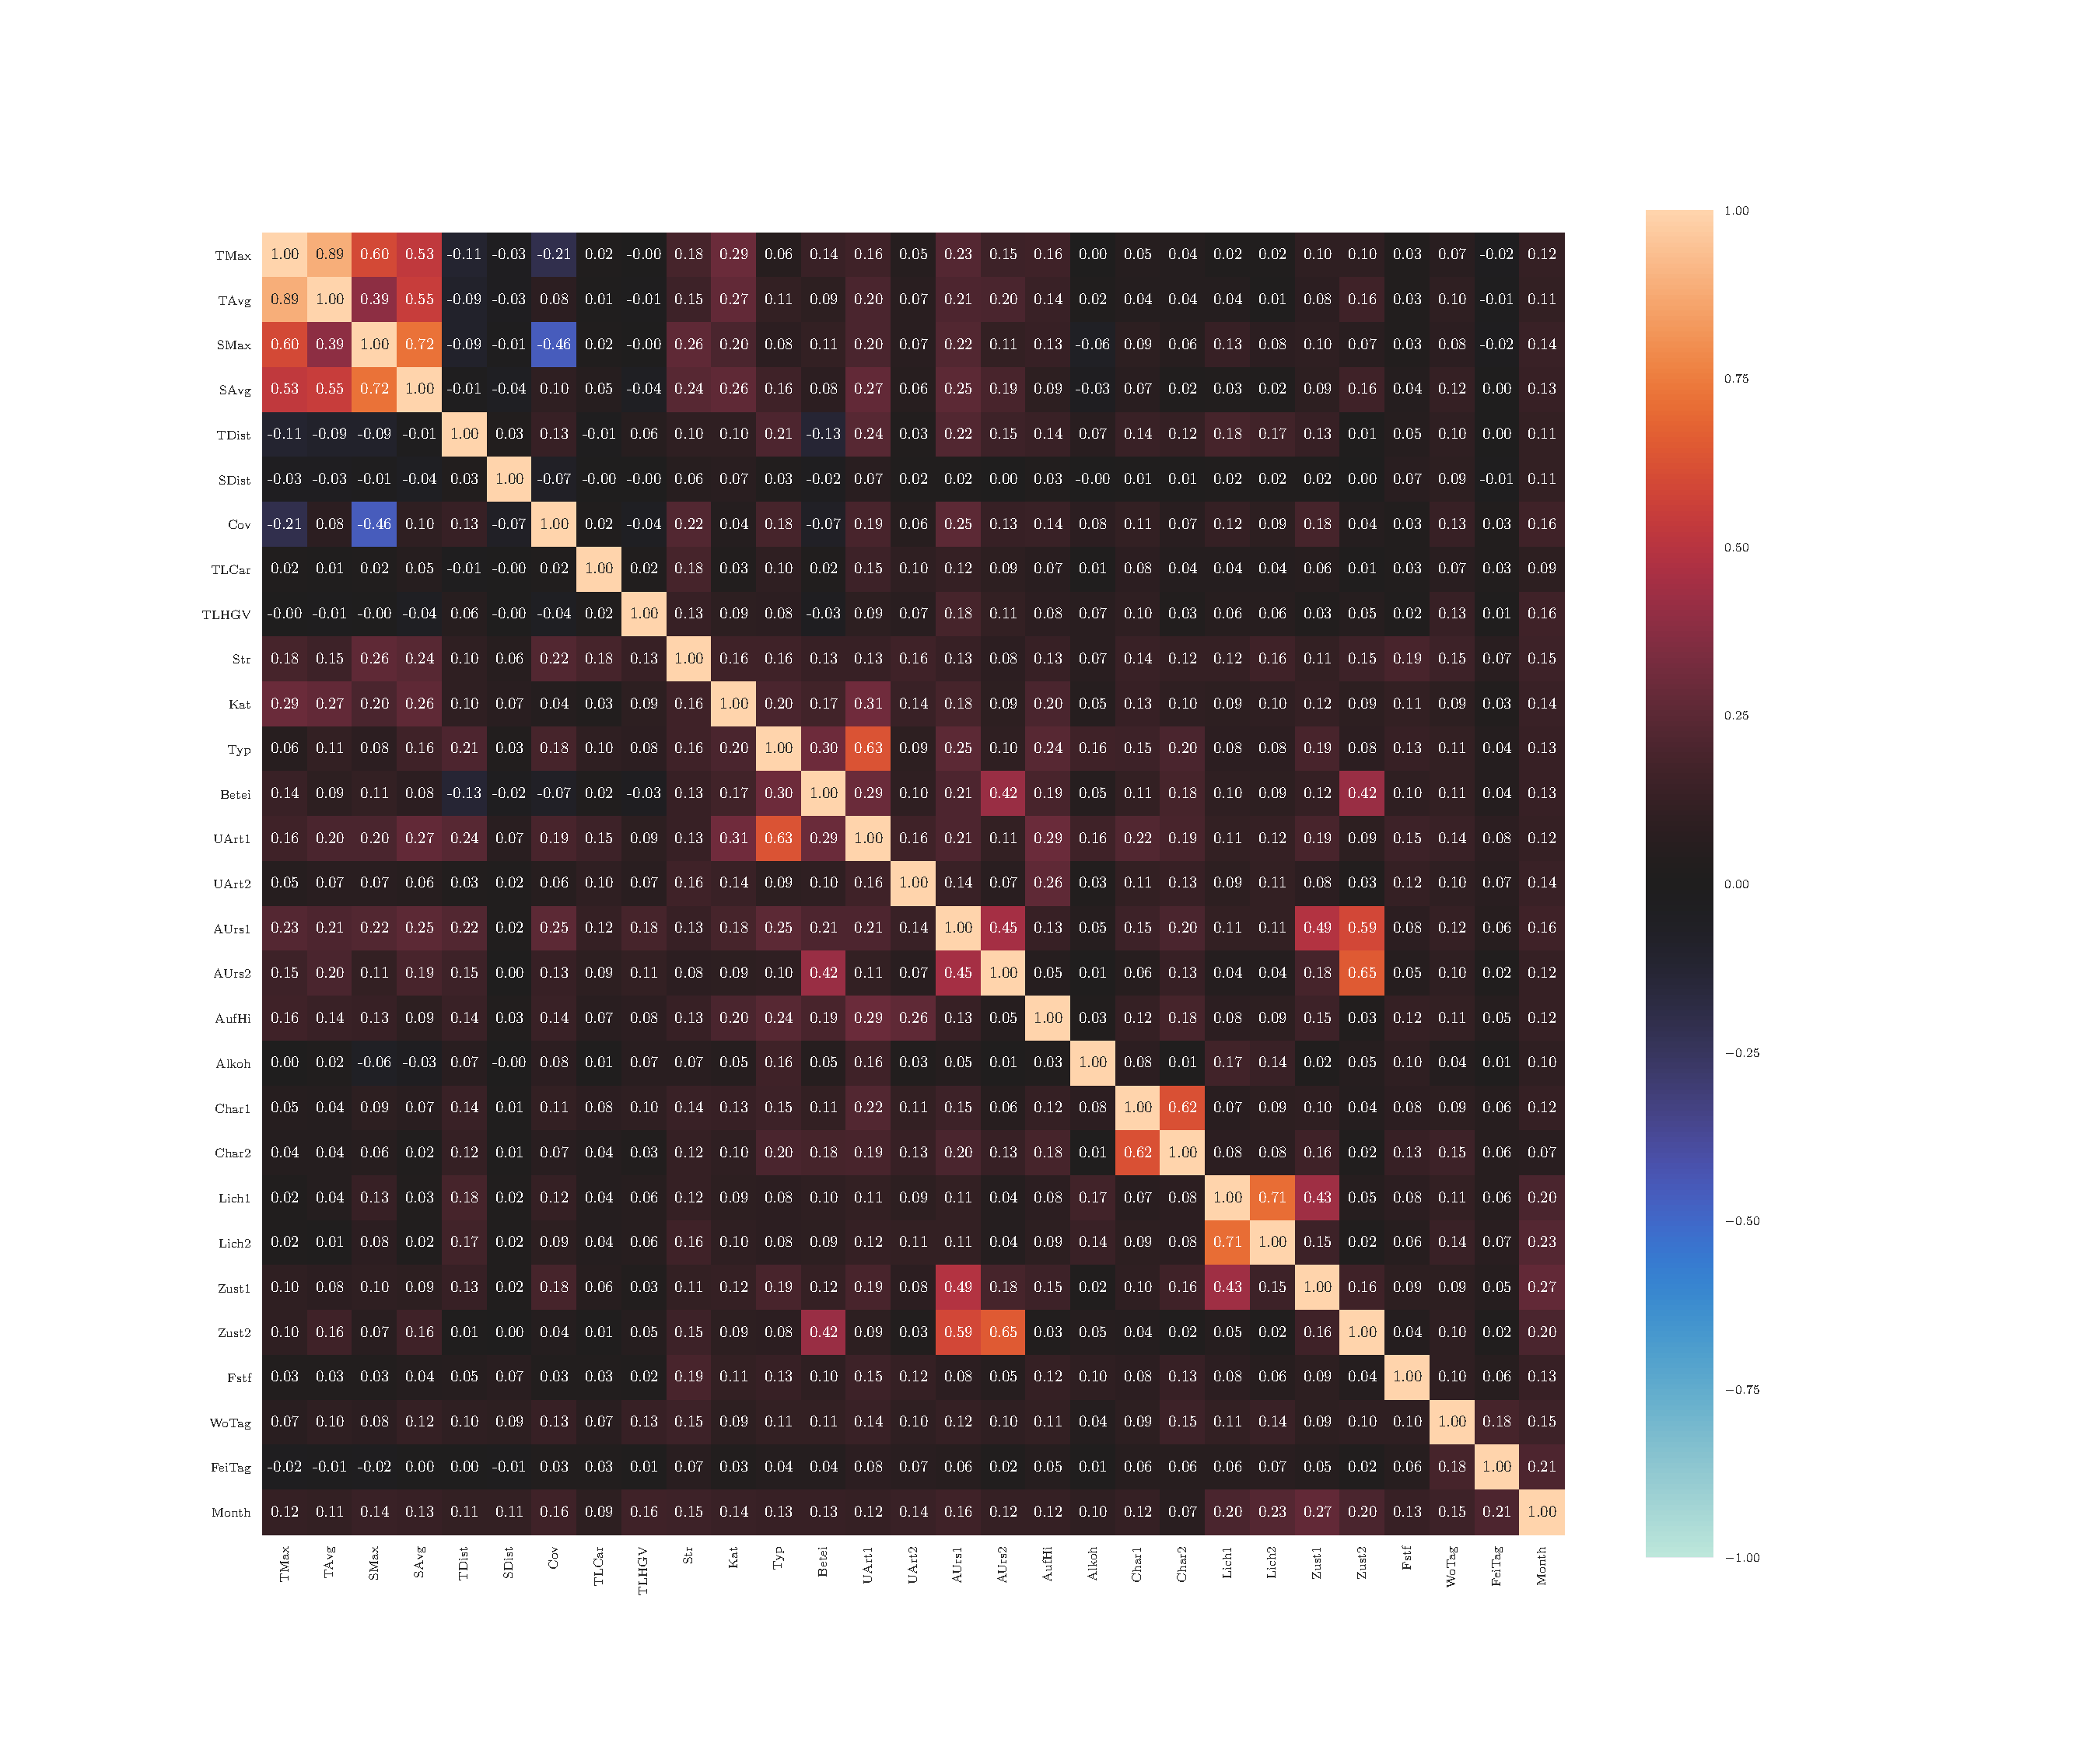
\includegraphics[width=1.4\textwidth, trim=0cm 2.5cm 6cm 3cm]{CorrAnalysis/data/BAYSIS/03_selected_01_startJam/plots/baysis_selected_corr_cramers}%
	}
	\caption{Correlation matrix for congestion-accident matched data classified as \textit{Jam Initiator} and calculated with $V$, $\eta$, $\tau$, $r_{pq}$, $r$}
	\label{img:correlation_matrix_selected_initiator_cramers}
\end{figure}

% --------------------------
% -------- Strasse ---------
% --------------------------
\centerheading{Strasse}
All of the Kruskal-Wallis rank sum test for \textit{Strasse} - \textit{TMax}, \textit{Strasse} - \textit{TAvg}, \textit{Strasse} - \textit{SMax}, \textit{Strasse} - \textit{SAvg}, \textit{Strasse} - \textit{Cov} and \textit{Strasse}-\textit{TLCar} produce a $p$-value above the defined $\alpha$-level of .05. This means that the correlation of the variable \textit{Strasse} can be neglected.

% ----------------------
% -------- Kat ---------
% ----------------------
\centerheading{Kat}
This section analyzes the correlated relations of the variable \textbf{Kat}. The encoding and description of the variable \textbf{Typ} is shown in \cref{tbl:baysis_dataset_Typ}.
% \begin{table}[!ht]
% 	\centering
% 	\tiny
% 	\begin{tabular}{c|l} 
% 		\toprule
% 		Code & Description \\ 
% 		\midrule
%  		0 	& Minor Accident  \\
%  		1 	& Accident with deaths  \\ 
%  		2 	& Accident with heavily injured  \\
%  		3 	& Accident with lightly injured  \\
% 		7 	& Accident with property damage  \\
% 		\bottomrule
% 	\end{tabular}
% 	\caption{Encoding of \textbf{Kat}}
% 	\label{table:analysis_encoding_Kat}
% 	%\vspace{-8mm}
% \end{table}
\paragraph{Maximal spatial Extent}
% chi-squared = 732.27, df = 720
The Kruskal-Wallis rank sum test of \textbf{Kat}-\textbf{SMax} produces a $p$-value of 0.3673, which is above $\alpha=.05$. The null hypothesis can't be rejected and there is no significant difference between the groups of \textbf{Kat}. There are no significant groups to identify.

\paragraph{Average spatial Extent}
% chi-squared = 738.37, df = 727
The Kruskal-Wallis rank sum test of \textbf{Kat}-\textbf{SAvg} produces a $p$-value of 0.3767, which is above $\alpha=.05$. The null hypothesis can't be rejected and there is no significant difference between the groups of \textbf{Kat}. There are no significant groups to identify.

\paragraph{Maximal Temporal Extent}
% chi-squared = 196.02, df = 131
The Kruskal-Wallis rank sum test of \textbf{Kat}-\textbf{TMax} produces a $p$-value of 0.0002, which is below $\alpha=.05$. The null hypothesis can therefore be rejected, which means there is a significant difference between the groups of \textbf{Kat}. To identify the significant groups, a pairwise Wilcoxon $T$-test for \textbf{Kat}-\textbf{TMax} is run, which produces \cref{tbl:wilcoxon_baysis_initiator_Kat_TMax}. 
\begin{table}[ht]
	\centering
	\begin{tabular}{rrrr}
		\toprule  
  		& 1 & 2 & 3 \\ 
  		\midrule    
        2 & 0.00 &  &  \\ 
        3 & 0.00 & 0.00 &  \\ 
        7 & 0.00 & 0.00 & 0.00 \\ 
 		\bottomrule
	\end{tabular}
    \caption{Pairwise Wilcoxon $T$-test for \textit{Kat} and \textit{Maximal Temporal Extent}}
    \label{tbl:wilcoxon_baysis_initiator_Kat_TMax}
\end{table}
The matrix shows that there is a general trend and all groups differ significantly. With the descriptives from \cref{tbl:descriptives_baysis_initiator_Kat_TMax} that the $\bar{x}$ and $\tilde{x}$ increases from group 7 to 1. We can therefore interpret that the maximal duration of jams, created by accidents increases with the gravity of the accident.
\begin{table}[ht]
	\centering
	\begin{tabular}{c|c|c|c|c|c|c|c}
		\toprule  
		Group & $n$ & $\bar{x}$ & $\sigma$ & $\tilde{x}$ & $min$ & $max$ & $\Delta$ \\
        \midrule
        1 & 29  & 290.07 & 190.59 & 255.00 & 27 & 864  & 837 \\ 
        2 & 144 & 156.23 & 119.44 & 120.00 & 9  & 657  & 648 \\ 
        3 & 423 & 121.05 & 105.34 & 99.00  & 9  & 1116 & 1107 \\ 
        7 & 181 & 103.13 & 143.89 & 75.00  & 9  & 1341 & 1332 \\ 
 		\bottomrule
	\end{tabular}
    \caption{Descriptives of the groups of \textit{Kat} and \textit{Maximal Temporal Extent} (Jam Initiator)}
    \label{tbl:descriptives_baysis_initiator_Kat_TMax}
\end{table}

\paragraph{Average temporal Extent}
% chi-squared = 222.52, df = 175
The Kruskal-Wallis rank sum test of \textbf{Kat}-\textbf{TAvg} produces a $p$-value of 0.0087, which is way below $\alpha=.05$. The null hypothesis can therefore be rejected, which means there is a significant difference between the groups of \textbf{Kat}. To identify the significant groups, a pairwise Wilcoxon $T$-test for \textbf{Kat}-\textbf{TAvg} is run, which produces \cref{tbl:wilcoxon_baysis_initiator_Kat_TAvg}. 
\begin{table}[ht]
	\small
	\centering
    \begin{tabular}{rrrr}
        \toprule
        & 1 & 2 & 3 \\ 
        \midrule
        2 & 0.00 &  &  \\ 
        3 & 0.00 & 0.01 &  \\ 
        7 & 0.00 & 0.00 & 0.00 \\ 
        \bottomrule
    \end{tabular}
	\caption{Pairwise Wilcoxon $T$-test for \textit{Kat} and \textit{Average Temporal Extent} (Jam Initiator)}
	\label{tbl:wilcoxon_baysis_initiator_Kat_TAvg}
\end{table}
The $p$-values show that all groups differ significantly from each other. The descriptives in table \cref{tbl:descriptives_baysis_initiator_Kat_TAvg}, show that $\bar{x}$ and $\tilde{x}$ increases with the groups from 7 to 1, like \textbf{TAMx}. The interpretation is therefore similar that the average duration of jams created by accident increases with the gravity of the accident.
\begin{table}[ht]
	\small
	\centering
    \begin{tabular}{c|c|c|c|c|c|c|c}
        \toprule
        Group & $n$ & $\bar{x}$ & $\sigma$ & $\tilde{x}$ & $min$ & $max$ & $\Delta$ \\
        \midrule
        1 & 29  & 148.76 & 90.65 & 144.00 & 20 & 376 & 356 \\ 
        2 & 144 & 80.91  & 67.52 & 61.50  & 7  & 426 & 419 \\ 
        3 & 423 & 63.84  & 51.24 & 53.00  & 5  & 469 & 464 \\ 
        7 & 181 & 53.61  & 80.96 & 39.00  & 4  & 920 & 916 \\ 
        \bottomrule
    \end{tabular}
	\caption{Group descriptives of \textit{Kat} and \textit{Average temporal Extent} (Jam Initiator)}
	\label{tbl:descriptives_baysis_initiator_Kat_TAvg}
	%\vspace{-8mm}
\end{table}

% ----------------------
% -------- Typ ---------
% ----------------------
\Large
\centerline{\textbf{Typ}}
\normalsize
This section analyzes the correlated relations of the accident variable \textbf{Typ} and introduces a initial interpretation of each significant correlation. Groups with an insufficient sample size (see \cref{correlation_uncertainty} are neglected and not considered. The encoding and description of the variable \textbf{Typ} is shown in \cref{tbl:baysis_dataset_Typ}. The relations of \textbf{Kat}-\textbf{SAvg} and 
\textbf{Kat}-\textbf{Cov} produce a $p$-value above the $\alpha$-level in the Kruskal-Wallis rank sum test. The null hypothesis can't therefore be rejected and there is no significant difference between the groups of \textbf{Typ} for these relations. The are also no significant groups to be identified for these relations.

The Kruskal-Wallis rank sum test of \textbf{Kat}-\textbf{TDist} produces a $p$-value of 0.0261, which is way below $\alpha=.05$. The null hypothesis can therefore be rejected, which means there is a significant difference between the groups of \textbf{Kat}. To identify the significant groups, a pairwise Wilcoxon $T$-test for \textbf{Kat}-\textbf{TDist} is run, which produces \cref{tbl:wilcoxon_baysis_initiator_Typ_TDist}. 
\begin{table}[ht]
	\tiny
	\centering
    \begin{tabular}{rrrrrr}
        \toprule
        & 1 & 3 & 4 & 5 & 6 \\ 
        \midrule
        3 & 0.05 &  &  &  &  \\ 
        4 & 1.00 & 0.38 &  &  &  \\ 
        5 & 0.96 & 1.00 & 0.96 &  &  \\ 
        6 & 0.00 & 0.96 & 0.51 & 1.00 &  \\ 
        7 & 1.00 & 0.04 & 1.00 & 0.96 & 0.01 \\ 
        \bottomrule
    \end{tabular}
    \caption{Pairwise Wilcoxon $T$-test for \textit{Typ} and \textit{Temporal Distance} (Jam Initiator)}
    \label{tbl:wilcoxon_baysis_initiator_Typ_TDist}
\end{table}
The significance matrix \cref{tbl:wilcoxon_baysis_initiator_Typ_TDist} shows that group 6 differs from group 1 and group 7 differs from 6. 
\begin{table}[ht]
	\tiny
	\centering
    \begin{tabular}{c|c|c|c|c|c|c|c}
        \toprule
        Group & $n$ & $\bar{x}$ & $\sigma$ & $\tilde{x}$ & $min$ & $max$ & $\Delta$ \\
        \midrule
        1 & 181 & 11.40 & 6.38 & 10.00 & 1  & 24 & 23 \\ 
        3 & 24  & 7.67  & 6.06 & 7.00  & 1  & 22 & 21 \\ 
        %4 & 4   & 14.00 & 3.92 & 13.50 & 10 & 19 & 9 \\ 
        %5 & 2   & 4.50  & 3.54 & 4.50  & 2  & 7  & 5 \\ 
        6 & 496 & 9.20  & 5.88 & 8.00  & 0  & 24 & 24 \\ 
        7 & 70  & 12.27 & 7.09 & 11.00 & 0  & 24 & 24 \\ 
        \bottomrule
    \end{tabular}
    \caption{Group descriptives of \textit{Typ} and \textit{Temporal Distance} (Jam Initiator)}
    \label{tbl:descriptives_baysis_initiator_Typ_TDist}
	%\vspace{-8mm}
\end{table}
The descriptives from \cref{tbl:descriptives_baysis_initiator_Typ_TDist} also shows that the temporal distance in group 1 and 7 is 25\,\% higher than in group 6. Group 3 also shows a substantial gap in $\bar{x}$ but only is barely significance with $p=.05$. Because the groups of $driving$ and $straight traffic$ accidents are very similar, there is no clear interpretation to be drawn.

% ------------------------
% -------- UArt1 ---------
% ------------------------
\centerheading{UArt}
This section analyzes the correlated relations of the accident variable \textbf{UArt} and introduces a initial interpretation of each significant correlation. Groups with an insufficient sample size (see \cref{correlation_uncertainty} are neglected and not considered. The encoding and description of the variable \textbf{UArt} is shown in \cref{tbl:baysis_dataset_UArt}. The Kruskal-Wallis rank sum test of \textbf{UArt1}-\textbf{TAvg}, \textbf{UArt1}-\textbf{SMax}, \textbf{UArt1}-\textbf{SAvg} and \textbf{UArt1}-\textbf{TLCar} produce $p$-values above the $\alpha$-level. This means that the null hypothesis can't be rejected and there is no significant difference between the groups of \textbf{UArt1} in these relations. 

The Kruskal-Wallis rank sum test of \textbf{UArt1}-\textbf{TMax} produces a $p$-value of 0.0015, which is below $\alpha=.05$. The null hypothesis can therefore be rejected, which means there is a significant difference between the groups of \textbf{UArt1}. To identify the significant groups, a pairwise Wilcoxon $T$-test for \textbf{UArt1}-\textbf{TMax} is run, which produces \cref{tbl:wilcoxon_baysis_initiator_UArt_TMax}. 
\begin{table}[ht]
	\tiny
	\centering
    \begin{tabular}{rrrrrrrrrr}
        \toprule
        & 0 & 1 & 2 & 3 & 4 & 5 & 6 & 7 & 8 \\ 
        \midrule
        1 & 1.00 &  &  &  &  &  &  &  &  \\ 
        2 & 1.00 & 1.00 &  &  &  &  &  &  &  \\ 
        3 & 1.00 & 0.04 & 0.00 &  &  &  &  &  &  \\ 
        4 & 1.00 & 1.00 & 1.00 & 1.00 &  &  &  &  &  \\ 
        5 & 1.00 & 1.00 & 1.00 & 1.00 & 1.00 &  &  &  &  \\ 
        6 & 1.00 & 1.00 & 1.00 & 1.00 & 1.00 & 1.00 &  &  &  \\ 
        7 & 0.75 & 0.05 & 0.12 & 1.00 & 1.00 & 1.00 & 1.00 &  &  \\ 
        8 & 1.00 & 0.21 & 0.43 & 1.00 & 1.00 & 1.00 & 1.00 & 1.00 &  \\ 
        9 & 1.00 & 0.43 & 1.00 & 1.00 & 1.00 & 1.00 & 1.00 & 1.00 & 1.00 \\ 
        \bottomrule
      \end{tabular}
    \caption{Pairwise Wilcoxon $T$-test for \textit{UArt1} and \textit{Maximal Temporal Extent} (Jam Initiator)}
    \label{tbl:wilcoxon_baysis_initiator_UArt_TMax}
\end{table}
It shows that only groups 4 and 7 differ significantly from group 1. 
\begin{table}[ht]
	\tiny
	\centering
    \begin{tabular}{c|c|c|c|c|c|c|c}
        \toprule
        Group & $n$ & $\bar{x}$ & $\sigma$ & $\tilde{x}$ & $min$ & $max$ & $\Delta$ \\
        \midrule
        % total: 777
        0 & 24  & 140.75 & 100.75 & 114.00 & 30 & 375  & 345 \\ 
        1 & 31  & 198.58 & 166.25 & 126.00 & 39 & 612  & 573 \\ 
        2 & 345 & 134.87 & 108.69 & 105.00 & 9  & 864  & 855  \\ 
        3 & 144 & 111.79 & 123.13 & 81.00  & 9  & 1116 & 1107 \\ 
        %4 & 4   & 186.00 & 145.68 & 175.50 & 39 & 354  & 315 \\ 
        5 & 15  & 179.60 & 324.31 & 99.00  & 15 & 1341 & 1326 \\ 
        %6 & 4   & 171.00 & 98.62  & 178.50 & 66 & 261  & 195 \\ 
        7 & 23  & 87.91  & 93.15  & 48.00  & 12 & 384  & 372 \\ 
        8 & 107 & 118.46 & 117.62 & 87.00  & 18 & 813  & 795 \\ 
        9 & 80  & 122.47 & 143.91 & 91.50  & 12 & 1152 & 1140 \\ 
        \bottomrule
      \end{tabular}
    \caption{Group descriptives of \textit{UArt1} and \textit{Maximal Temporal Extent} (Jam Initiator)}
    \label{tbl:descriptives_baysis_initiator_UArt_TMax}
	%\vspace{-8mm}
\end{table}
Because group 4 only contains 4 samples (see \cref{tbl:descriptives_baysis_initiator_UArt_TMax}) it is considered uncertain (see \cref{correlation_uncertainty}).

The Kruskal-Wallis rank sum test of \textbf{UArt1}-\textbf{TDist} produces a $p$-value of 0.0084, which is below $\alpha=.05$. The null hypothesis can therefore be rejected, which means there is a significant difference between the groups of \textbf{UArt1}. To identify the significant groups, a pairwise Wilcoxon $T$-test for \textbf{UArt1}-\textbf{TDist} is run, which produces \cref{tbl:wilcoxon_baysis_initiator_UArt_TDist}. 
\begin{table}[ht]
	\tiny
	\centering
    \begin{tabular}{rrrrrrrrrr}
        \toprule
        & 0 & 1 & 2 & 3 & 4 & 5 & 6 & 7 & 8 \\ 
        \midrule
        1 & 1.00 &  &  &  &  &  &  &  &  \\ 
        2 & 1.00 & 1.00 &  &  &  &  &  &  &  \\ 
        3 & 1.00 & 1.00 & 1.00 &  &  &  &  &  &  \\ 
        4 & 1.00 & 1.00 & 1.00 & 1.00 &  &  &  &  &  \\ 
        5 & 1.00 & 1.00 & 1.00 & 1.00 & 1.00 &  &  &  &  \\ 
        6 & 1.00 & 1.00 & 1.00 & 1.00 & 1.00 & 1.00 &  &  &  \\ 
        7 & 1.00 & 0.06 & 0.00 & 0.00 & 1.00 & 0.10 & 1.00 &  &  \\ 
        8 & 1.00 & 1.00 & 0.01 & 0.01 & 1.00 & 1.00 & 1.00 & 1.00 &  \\ 
        9 & 1.00 & 1.00 & 0.05 & 0.01 & 1.00 & 0.78 & 1.00 & 0.87 & 1.00 \\ 
        \bottomrule
      \end{tabular}
    \caption{Pairwise Wilcoxon $T$-test for \textit{UArt1} and \textit{Temporal Distance} (Jam Initiator)}
    \label{tbl:wilcoxon_baysis_initiator_UArt_TDist}
\end{table}
The table shows, that groups 7, 8 and 9 differ from group 2 and 3.
\begin{table}[ht]
	\tiny
	\centering
    \begin{tabular}{c|c|c|c|c|c|c|c}
        \toprule
        Group & $n$ & $\bar{x}$ & $\sigma$ & $\tilde{x}$ & $min$ & $max$ & $\Delta$ \\
        \midrule
        0 & 24  & 11.04 & 6.22 & 10.00 & 2  & 22 & 20 \\ 
        1 & 31  & 8.94  & 6.03 & 7.00  & 0  & 24 & 24 \\ 
        2 & 345 & 9.21  & 5.90 & 8.00  & 1  & 24 & 23 \\ 
        3 & 144 & 8.80  & 6.03 & 7.00  & 1  & 24 & 23 \\ 
        %4 & 4   & 12.00 & 4.08 & 10.50 & 9  & 18 & 9  \\ 
        5 & 15  & 8.13  & 7.06 & 7.00  & 0  & 22 & 22 \\ 
        %6 & 4   & 14.00 & 3.92 & 13.50 & 10 & 19 & 9  \\ 
        7 & 23  & 15.26 & 7.04 & 14.00 & 4  & 24 & 20 \\ 
        8 & 107 & 11.81 & 6.57 & 11.00 & 1  & 24 & 23 \\ 
        9 & 80  & 11.38 & 5.87 & 10.00 & 2  & 24 & 22 \\ 
        \bottomrule
      \end{tabular}
    \caption{Group descriptives of \textit{UArt1} and \textit{Temporal Distance}}
    \label{tbl:descriptives_baysis_initiator_UArt_TDist}
	%\vspace{-8mm}
\end{table}
In consideration of the descriptives in \cref{tbl:descriptives_baysis_initiator_UArt_TDist} it can be interpreted that accidents with \textit{obstacles collision}, \textit{deviations to the right} and \textit{deviations to the left} have a longer (temporal) reaction (see distribution of $\bar{x}$) to create a jam than accident with ahead vehicles.

The Kruskal-Wallis rank sum test of \textbf{UArt1}-\textbf{Cov} produces a $p$-value of 0.0337, which is below $\alpha$-level. The null hypothesis can therefore be rejected, which means there are significant differences in \textbf{UArt}. To identify the significant groups the a pairwise Wilcoxon $T$-test for \textbf{UArt1}-\textbf{Cov}, produces \cref*{tbl:wilcoxon_baysis_initiator_UArt_Cov}. It shows that the significant differences are not related to any specific group of \textbf{UArt1} and the correlation can be neglected.
\begin{table}[ht]
	\tiny
	\centering
    \begin{tabular}{rrrrrrrrrr}
        \toprule
        & 0 & 1 & 2 & 3 & 4 & 5 & 6 & 7 & 8 \\ 
        \midrule
        1 & 1.00 &  &  &  &  &  &  &  &  \\ 
        2 & 1.00 & 1.00 &  &  &  &  &  &  &  \\ 
        3 & 1.00 & 1.00 & 1.00 &  &  &  &  &  &  \\ 
        4 & 1.00 & 1.00 & 1.00 & 1.00 &  &  &  &  &  \\ 
        5 & 1.00 & 1.00 & 1.00 & 1.00 & 1.00 &  &  &  &  \\ 
        6 & 1.00 & 1.00 & 1.00 & 1.00 & 1.00 & 1.00 &  &  &  \\ 
        7 & 1.00 & 1.00 & 1.00 & 1.00 & 1.00 & 1.00 & 1.00 &  &  \\ 
        8 & 1.00 & 1.00 & 0.12 & 0.09 & 1.00 & 0.72 & 1.00 & 1.00 &  \\ 
        9 & 1.00 & 1.00 & 1.00 & 1.00 & 1.00 & 1.00 & 1.00 & 1.00 & 1.00 \\ 
        \bottomrule
      \end{tabular}
    \caption{Pairwise Wilcoxon $T$-test for \textit{UArt1} and \textit{Coverage} (Jam Initiator)}
    \label{tbl:wilcoxon_baysis_initiator_UArt_Cov}
\end{table}

% ------------------------
% -------- AUrs1 ---------
% ------------------------
\centerheading{AUrs}
This section analyzes the correlated relations of the accident variable \textbf{AUrs1} and \textbf{AUrs2}, also introducing a initial interpretation of each significant correlation. Groups with an insufficient sample size (see \cref{correlation_uncertainty} are neglected and not considered. The encoding and description of the variable \textbf{AUrs} is shown in \cref{tbl:baysis_dataset_AUrs}. The Kruskal-Wallis rank sum test of \textbf{AUrs1}-\textbf{TMax}, \textbf{AUrs1}-\textbf{TAvg}, \textbf{AUrs1}-\textbf{SMax}, \textbf{AUrs1}-\textbf{SAvg}, \textbf{AUrs1}-\textbf{TDist} and \textbf{AUrs1}-\textbf{TLCar} produce $p$-values above the $\alpha$-level. This means that the null hypothesis can't be rejected and there is no significant difference between the groups of \textbf{UArt1} in these relations. 

The Kruskal-Wallis rank sum test of \textbf{AUrs1}-\textbf{Cov} produces a $p$-value of 0.0176, which is below $\alpha=.05$. The null hypothesis can therefore be rejected, pointing to a significant difference between the groups of \textbf{AUrs1}. The pairwise Wilcoxon $T$-test of \textbf{AUrs1}-\textbf{Cov} for identification of the relevant groups (see \cref{tbl:wilcoxon_baysis_initiator_AUrs1_Cov}) shows that the significance differences is not group specific. The correlation can therefore be neglected.
\begin{table}[ht]
	\small
	\centering
    \begin{tabular}{rrrrrrrrrrrrr}
        \toprule
           & 72 & 73 & 75 & 77 & 81 & 82 & 83 & 84 & 86 & 87 & 88 \\ 
        \midrule
        72 &  &  &  &  &  &  &  &  &  &  &  \\ 
        73 & 0.63 &  &  &  &  &  &  &  &  &  &  \\ 
        75 & 1.00 & 1.00 &  &  &  &  &  &  &  &  &  \\ 
        77 & 1.00 & 1.00 & 1.00 &  &  &  &  &  &  &  &  \\ 
        81 & 1.00 & 1.00 & 1.00 & 1.00 &  &  &  &  &  &  &  \\ 
        82 & 1.00 & 1.00 & 1.00 & 1.00 & 1.00 &  &  &  &  &  &  \\ 
        83 & 1.00 & 1.00 & 1.00 & 1.00 & 1.00 & 1.00 &  &  &  &  &  \\ 
        84 & 1.00 & 1.00 & 1.00 & 1.00 & 1.00 & 1.00 & 1.00 &  &  &  &  \\ 
        86 & 1.00 & 1.00 & 1.00 & 1.00 & 1.00 & 1.00 & 1.00 & 1.00 &  &  &  \\ 
        87 & 1.00 & 1.00 & 1.00 & 1.00 & 1.00 & 1.00 & 1.00 & 1.00 & 1.00 &  &  \\ 
        88 & 1.00 & 1.00 & 1.00 & 1.00 & 1.00 & 1.00 & 1.00 & 1.00 & 1.00 & 1.00 &  \\ 
        89 & 0.33 & 0.96 & 1.00 & 1.00 & 1.00 & 1.00 & 1.00 & 1.00 & 0.91 & 1.00 & 1.00 \\ 
        \bottomrule
    \end{tabular}
    \caption{Pairwise Wilcoxon $T$-test for \textit{AUrs1} and \textit{Coverage} (Jam Initiator)}
    \label{tbl:wilcoxon_baysis_initiator_AUrs1_Cov}
\end{table}

% ------------------------
% -------- AUrs2 ---------
% ------------------------
\medskip
All relations of the second \textbf{AUrs} variable \textbf{AUrs2} (\textbf{AUrs2}-\textbf{TMax}, \textbf{AUrs2}-\textbf{TAvg}, \textbf{AUrs2}-\textbf{SAvg} and \textbf{AUrs2}-\textbf{TDist}) produce $p$-values above $\alpha$-level. The null hypothesizes can't be rejected and there is no significant differences between the groups of \textbf{AUrs2}. There are therefore no significant groups to identify.

% ------------------------
% -------- AufHi ---------
% ------------------------
\centerheading{AufHi}
This section analyzes the correlated relations of the accident variable \textit{AufHi}. The relations of \textit{AufHi}-\textit{TAvg} and \textit{AufHi}-\textit{Cov} produce a $p$-value above the $\alpha$-level. The null hypothesizes can't be rejected and there are no significant differences between the groups of \textit{AufHi} for these relations.

The Kruskal-Wallis rank sum tests of \textit{AufHi} - \textit{TMax} produces a $p$-value of 0.0411, which is below $\alpha=.05$. The null hypothesis can therefore be rejected, which means there is a significant difference between the groups of \textit{AufHi}. The pairwise Wilcoxon $T$-test for \textit{AufHi} - \textit{TMax} shows no significant differences between the groups, which mean that the correlation can be neglected.

The Kruskal-Wallis rank sum test of \textit{AufHi} - \textit{TDist} produces a $p$-value of 0.0007, which is below $\alpha=.05$. The null hypothesis can therefore be rejected, which means there is a significant difference between the groups of \textit{AufHi}. The pairwise Wilcoxon $T$-test for \textit{AufHi} - \textit{TDist} shows no significant differences between the groups.

% ------------------------
% -------- Char1 ---------
% ------------------------
\centerheading{Char}
This section analyzes the correlated relations of the accident variable \textit{Char}. The relations of \textit{Char1}-\textit{TDist} produces a $p$-value above the $\alpha$-level. The null hypothesis can't be rejected and there is no significant difference between the groups of \textit{Char1}. There are therefore also no significant groups to identify.

% --------------------------------
% -------- Lich1 & Lich2 ---------
% --------------------------------
\centerheading{Lich}
This section analyzes the correlated relations of the accident variable \textit{Lich1} as well as \textit{Lich2}. The relations of \textit{Lich1}-\textit{TDist} and \textit{Lich2}-\textit{TDist} produce a $p$-value above the $\alpha$-level. The null hypothesizes can't be rejected and there are no significant differences between the groups of \textit{Lich1} and \textit{Lich2}.

% ------------------------
% -------- Zust1 ---------
% ------------------------
\centerheading{Zust}
This section analyzes the correlated relations of the accident variable \textit{Zust1}/\textit{Zust2} and introduces a initial interpretation of each significant correlation. The encoding and description of the variable \textit{Zust} is shown in \cref{tbl:baysis_dataset_Zust}. The relations of \textit{Zust2} - \textit{SAvg} produce a $p$-value above $\alpha=.05$. The null hypothesizes can't be rejected and there are no significant differences between the groups of \textit{Zust2}. The Kruskal-Wallis rank sum test of \textit{Zust2} - \textit{TAvg} produces a $p$-value of < 0.0001, which is significant. But because the distribution only contains a single values, there are no interpretations to be draw and the correlation can be neglected.

The Kruskal-Wallis rank sum test of \textit{Zust1} - \textit{Cov} produces a $p$-value of 0.0046, which is way below $\alpha=.05$. The null hypothesis can therefore be rejected, which means there is a significant difference between the groups of \textit{Zust1}. To identify the significant groups, a pairwise Wilcoxon $T$-test for \textit{Zust1} - \textit{Cov} is run, which produces \cref{tbl:wilcoxon_baysis_initiator_Zust1_Cov}. 
\begin{table}[ht!]
	\tiny
	\centering
    \begin{tabular}{rrrr}
        \toprule
          & 0 & 1 \\ 
        \midrule
        0 &      & \\ 
        1 & 0.04 & \\ 
        2 & 0.00 & 0.01 \\ 
        \bottomrule
      \end{tabular}
    \caption{Pairwise Wilcoxon $T$-test for \textit{Zust1} and \textit{Coverage}}
    \label{tbl:wilcoxon_baysis_initiator_Zust1_Cov}
\end{table}
The table shows that all groups differ significantly, which means that there is a general trend.
\begin{table}[ht!]
	\tiny
	\centering
    \begin{tabular}{c|c|c|c|c|c|c|c}
        \toprule
        Group & $n$ & $\bar{x}$ & $\sigma$ & $\tilde{x}$ & $min$ & $max$ & $\Delta$ \\
        \midrule
        0 & 548 & 50.80 & 20.28 & 49.50 & 6  & 100 & 94 \\ 
        1 & 208 & 55.35 & 21.35 & 55.00 & 5  & 100 & 95 \\ 
        2 & 18  & 74.06 & 26.80 & 87.50 & 18 & 100 & 82 \\ 
        \bottomrule
      \end{tabular}
    \caption{Group descriptives of \textit{Zust1} and \textit{Coverage}}
    \label{tbl:descriptives_baysis_initiator_Zust1_Cov}
	%\vspace{-8mm}
\end{table}
With the descriptives in \cref*{tbl:descriptives_baysis_initiator_Zust1_Cov} it can be interpreted that the coverage of the jam increases from \textit{dry} over \textit{wet} to \textit{ice} by nearly 50\,\%.

% ------------------------
% -------- Month ---------
% ------------------------
\centerheading{Month}
This section analyzes the correlated relations of the accident variable \textit{Month}. The relations of \textit{Month} - \textit{TMax}, \textit{Month} - \textit{Cov} and \textit{Month} - \textit{TLHGV} produce a $p$-value above the $\alpha$-level. The null hypothesizes can't be rejected and there are \textit{no} significant differences between the groups of \textit{Month} for the mentioned relations. There are no significant groups to identify.
\clearpage
% % Effector
% ----------------------------------------------------
% -------- BAYSIS - Selected as Jam Effector ---------
% ----------------------------------------------------
\subsection{Congestion - Accidents categorizes as Jam Effector}
\label{analysis_processing_correlation_baysis_effector}
The correlation matrix table for the congestion - accident dataset, which are classified as \textit{Jam Effector} (see \cref{table:appendix_correlation_matrix_matched_cramers}) is visual presented in \cref{img:correlation_matrix_selected_effector_cramers} showing the the correlation of each variable combination. When visual analyzing \cref{img:correlation_matrix_matched_cramers} and checking the guidelines for a strong correlation in reference to the applied coefficient (identifiable with \cref{table:appendix_coefficient_matrix_matched}) we get a list of strongly correlated variable combinations (see \cref{tbl:correlation_list_baysis_effector}). Since the focus of the thesis are the correlations between accidents and jams, these are only collected from the bottom-left rectangle of the matrix, where the congestion and accidents variables intersect. Correlations of the kind congestion - congestion or accident - accident are not considered.
\begin{table}[h!]
	\centering
	\begin{tabular}{c|l}  
		Category & Strong \\
		\\[-1em]
		\hline
		\\[-1em]
		Strasse & TMax, TAvg, SMax, SAvg, Cov, TLHGV \\ 
 		Kat & TMax, TAvg, SAvg \\ % + SMax % -> Strasse
 		%Typ & \\ % -> Strasse
 		%Betei & \\
 		UArt1 & SAvg \\ % -> Strasse
 		%UArt2 & \\ % -> Strasse
 		%AUrs1 & \\ % -> Strasse
 		%AUrs2 & \\
 		AufHi & TMax, TAvg \\
 		%Alkoh & \\
 		%Char1 & \\ % -> Strasse
 		%Char2 & \\ % -> Strasse
 		%Lich1 & \\ % -> Strasse
 		%Lich2 & \\ % -> Strasse
 		%Zust1 & \\ % -> Strasse
 		%Zust2 & \\ % -> Strasse
 		%Fstf & \\ % -> Strasse
 		WoTag & TAvg, SMax, Cov, TLHGV \\ % -> Strasse
 		%FeiTag & \\
 		Month & TMax, TAvg, SMax, SAvg, Cov, TLHGV \\ % -> Strasse
	\end{tabular}
    \caption{List of incident variables and their strong correlated congestion variable from the congestion-accident matched data which are classified as \textit{Jam Effector}}
	\label{tbl:correlation_list_baysis_effector}
\end{table}
Next we need to verify that the correlation is significant and what the correlation predicates. Therefore each correlation will be evaluated with the Post Hoc test, defined in \cref{correlation_posthoc}. \secintroend{baysis}{effector}
\begin{figure}[!ht]
	\centering
	\makebox[\textwidth][c]{%
		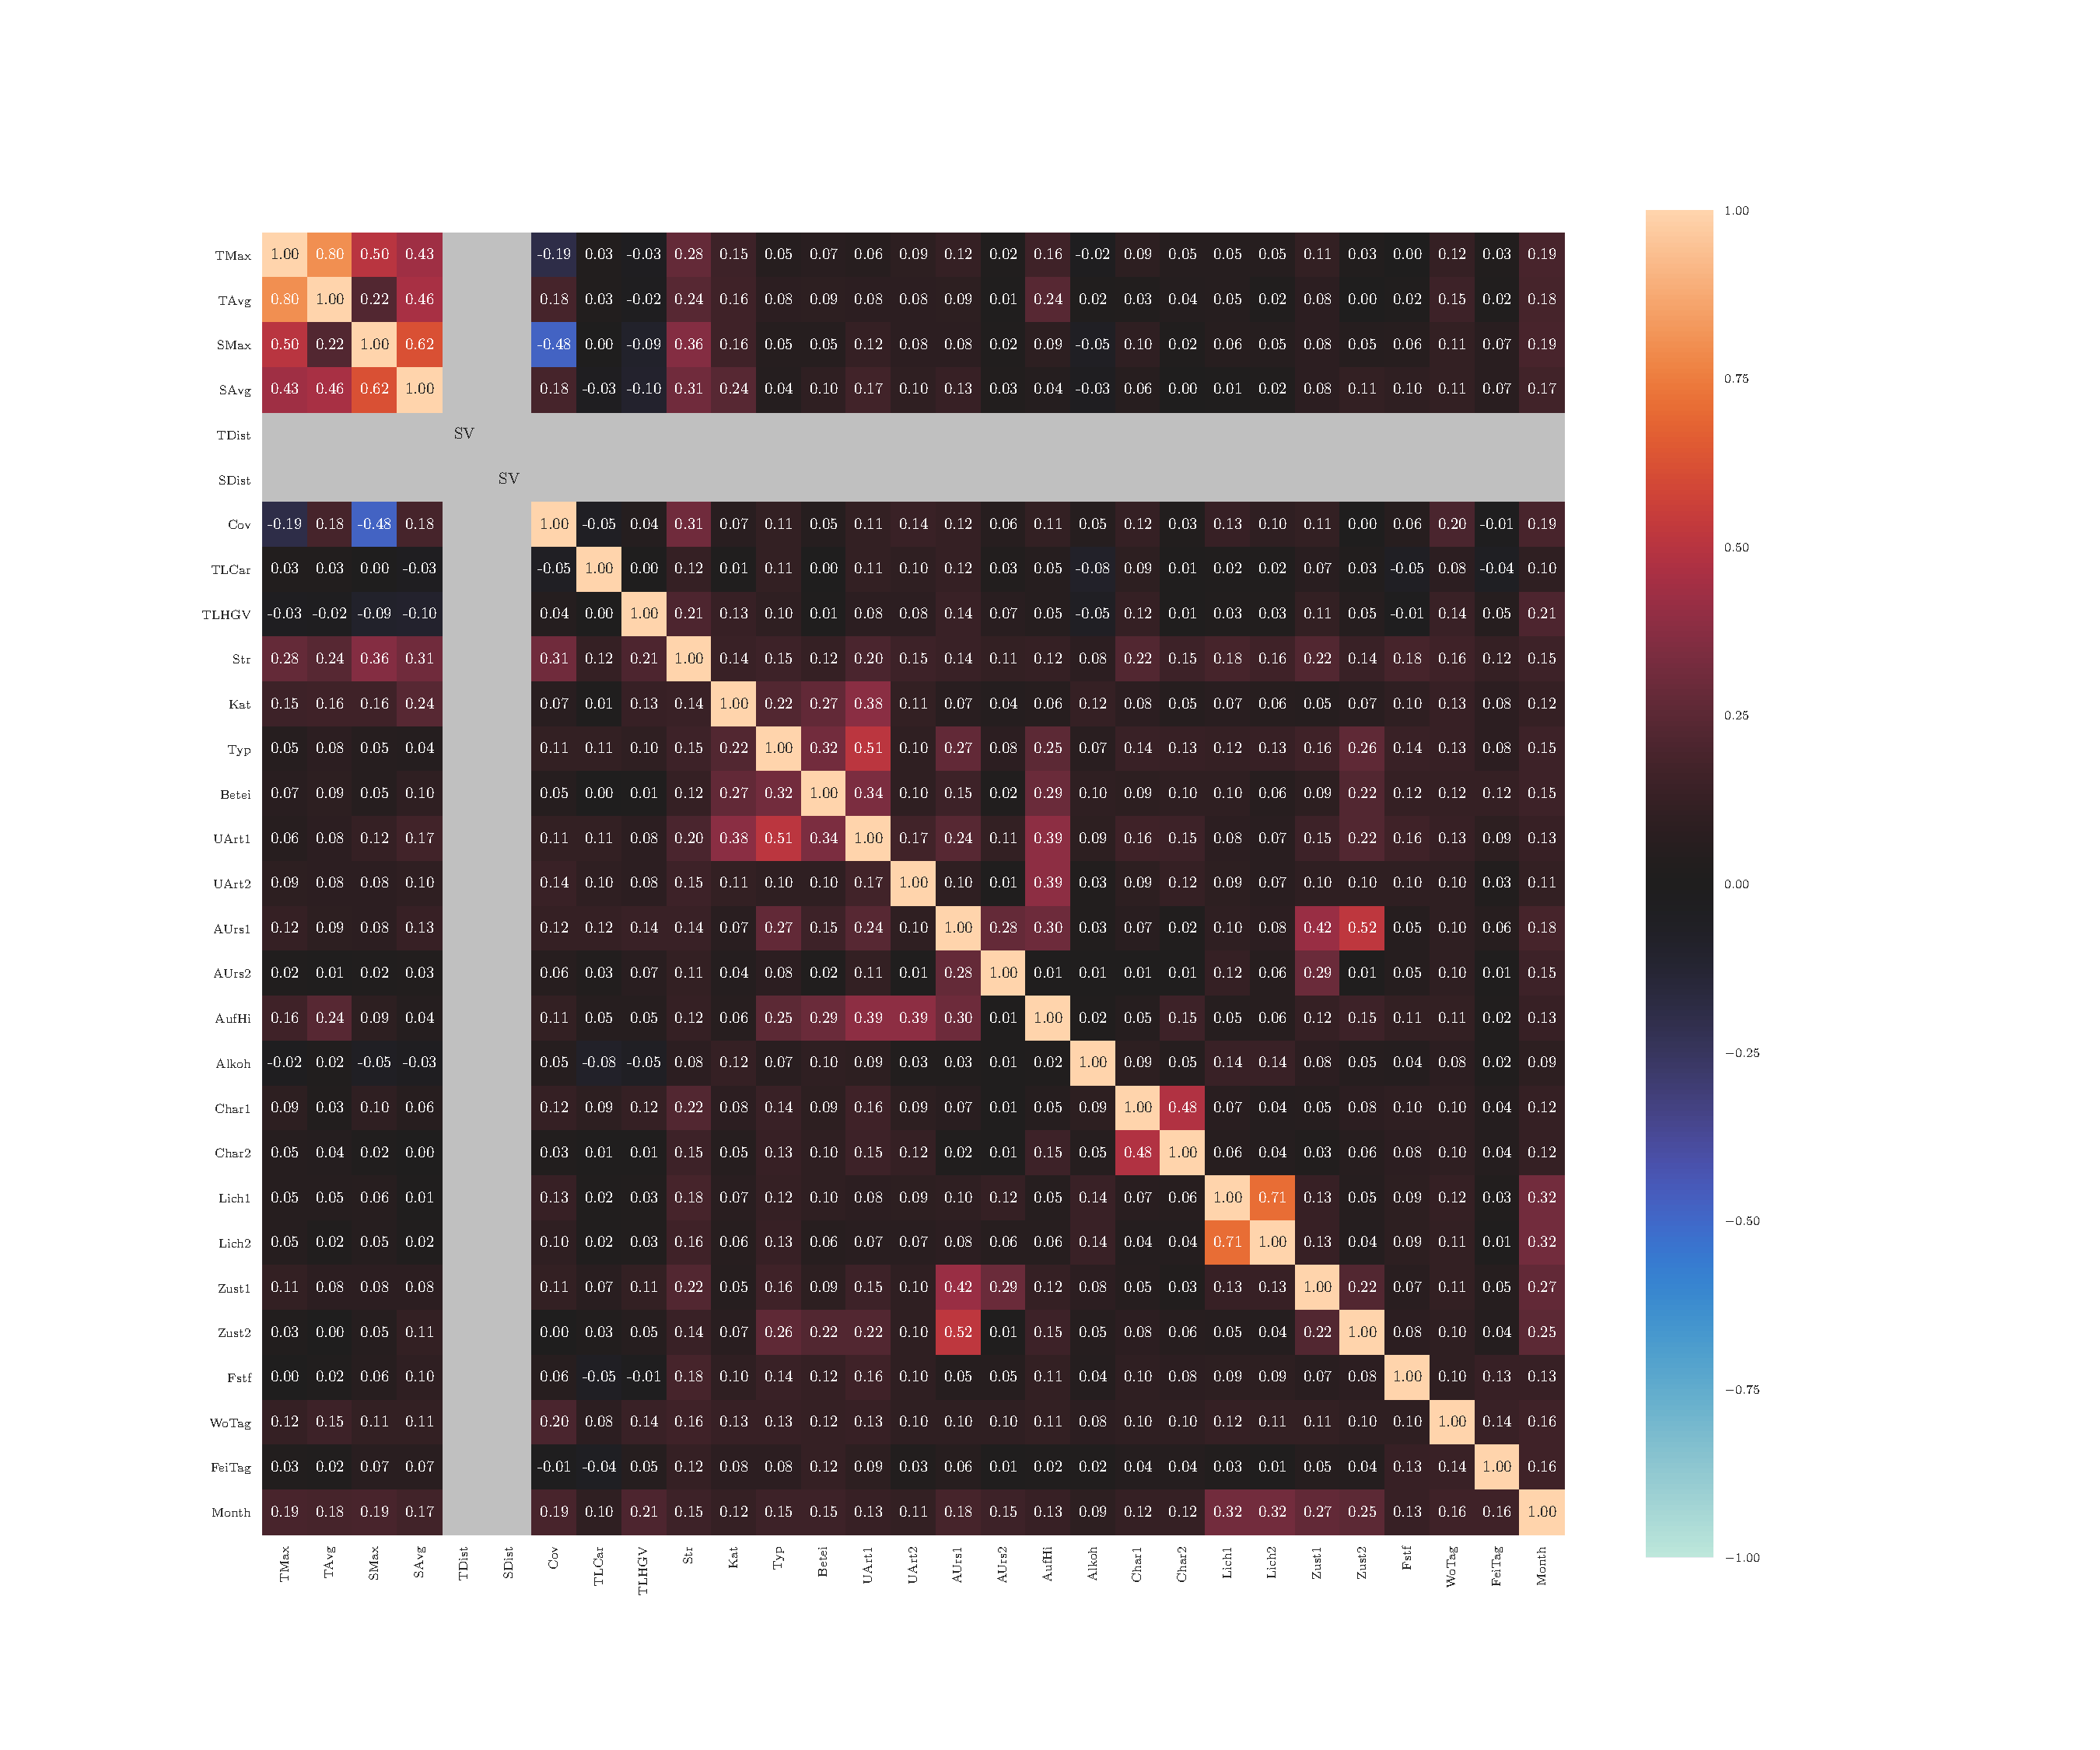
\includegraphics[width=1.4\textwidth, trim=0cm 2.5cm 6cm 3cm]{CorrAnalysis/data/BAYSIS/03_selected_02_duringJam/plots/baysis_selected_corr_cramers}%
	}
	\caption{Correlation matrix for congestion-accident matched data classified as \textit{Jam Effector} and calculated with $V$, $\eta$, $\tau$, $r_{pq}$, $r$}
	\label{img:correlation_matrix_selected_effector_cramers}
\end{figure}

% --------------------------
% -------- Street ---------
% --------------------------
\centerheading{Street}
\label{ana:baysis_effector_Str}
\varintrosimplewithsam{Str}
\varintronosigmul{Str}{\textit{Strasse} - \textit{SAvg} and \textit{Strasse} - \textit{TLHGV}}

% #################################################
\groupintrosig{Street}{TMax}{0.0104}{baysis}{effector}
\begin{table}[ht!]
	\tiny
	\centering
	\begin{tabular}{rrrrrrrrrrrrrr}
		\toprule
		     & A3 & A6 & A9 & A70 & A99 & A93 & A94 & A7 & A73 & A96 & A995 & A92 & A95 \\ 
		\midrule
		% A6   & 1.00 &  &  &  &  &  &  &  &  &  &  &  &  \\ 
		% A9   & 1.00 & 1.00 &  &  &  &  &  &  &  &  &  &  &  \\ 
		% A70  & 1.00 & 1.00 & 1.00 &  &  &  &  &  &  &  &  &  &  \\ 
		% A99  & 0.85 & 1.00 & 1.00 & 1.00 &  &  &  &  &  &  &  &  &  \\ 
		% A93  & 1.00 & 1.00 & 1.00 & 1.00 & 1.00 &  &  &  &  &  &  &  &  \\ 
		A94  & \red{0.01} & 1.00 & 0.06 & 1.00 & 0.28 & 1.00 &  &  &  &  &  &  &  \\ 
		% A7   & .00 & 1.00 & 1.00 & 1.00 & 1.00 & 1.00 & 1.00 &  &  &  &  &  &  \\ 
		A73  & \red{0.00} & 1.00 & \red{0.00} & 1.00 & 0.23 & 1.00 & 1.00 & 1.00 &  &  &  &  &  \\ 
		A96  & \red{0.00} & 1.00 & 0.35 & 1.00 & 1.00 & 1.00 & 1.00 & 1.00 & 1.00 &  &  &  &  \\ 
		% A995 & 1.00 & 1.00 & 1.00 & 1.00 & 1.00 & 1.00 & 1.00 & 1.00 & 1.00 & 1.00 &  &  &  \\ 
		A92  & \red{0.01} & 1.00 & 0.24 & 1.00 & 1.00 & 1.00 & 1.00 & 1.00 & 1.00 & 1.00 & 1.00 &  &  \\ 
		% A95  & 1.00 & 1.00 & 1.00 & 1.00 & 1.00 & 1.00 & 1.00 & 1.00 & 1.00 & 1.00 & 1.00 & 1.00 &  \\ 
		% A980 & 1.00 & 1.00 & 1.00 & 1.00 & 1.00 & 1.00 & 1.00 & 1.00 & 1.00 & 1.00 & 1.00 & 1.00 &  \\ 
		\bottomrule
	  \end{tabular}
    \caption{Pairwise Wilcoxon $T$-test for \textit{Street} and \textit{Maximal Temporal Extent} (Jam Effector)}
    \label{tbl:wilcoxon_baysis_effector_Street_TMax}
\end{table}
The table shows that the roads A73, A94, A95 and A96 differ from the A3. The A73 also differs from the A9, but there is no distinctive general trend.
% #### START: Table and Plot
\begin{figure}[ht!]
	\centering
	\begin{minipage}{0.5\textwidth}
		\tiny
		\setlength{\tabcolsep}{4pt}
		\centering
		\begin{tabular}{c|c|c|c|c|c|c|c}
			\toprule
			Group & $n$ & $\bar{x}$ & $\sigma$ & $\tilde{x}$ & $min$ & $max$ & $\Delta$ \\
			\midrule
			A3   & 265 & 297.62 & 219.09 & 243.0 & 18 & 1257 & 1239 \\ 
			A6   & 37  & 236.59 & 183.03 & 207.0 & 18 & 705  & 687  \\ 
			A9   & 192 & 243.45 & 178.97 & 201.0 & 15 & 1194 & 1179 \\ 
			A99  & 63  & 212.57 & 140.78 & 195.0 & 21 & 681  & 660  \\ 
			A93  & 12  & 212.00 & 187.74 & 130.5 & 39 & 588  & 549  \\ 
			A94  & 14  & 109.71 & 56.07  & 97.5  & 42 & 249  & 207  \\ 
			A7   & 35  & 254.66 & 306.21 & 168.0 & 42 & 1341 & 1299 \\ 
			A73  & 52  & 157.21 & 179.42 & 130.5 & 18 & 1323 & 1305 \\ 
			A96  & 41  & 155.85 & 84.33  & 144.0 & 30 & 381  & 351  \\ 
			A92  & 21  & 134.71 & 82.25  & 138.0 & 18 & 354  & 336  \\ 
			\bottomrule
			% \bar{x} - sum = 2014.37, mean = 201,43
			% \sigma - sum = 1617.89, mean = 161.78
			% \tilde{x}
		\end{tabular}
		\subcaption[second caption.]{Table of all descriptives}\label{tbl:descriptives_baysis_effector_Street_TMax}
	\end{minipage}%
	\begin{minipage}{0.55\textwidth}
		\pgfplotstableread[col sep=comma]{
			road, count, mean, median, sd, min, max, delta
			A3   , 265 , 297.62 , 219.09 , 243.0 , 18 , 1257 , 1239
			A6   , 37  , 236.59 , 183.03 , 207.0 , 18 , 705  , 687 
			A9   , 192 , 243.45 , 178.97 , 201.0 , 15 , 1194 , 1179
			A99  , 63  , 212.57 , 140.78 , 195.0 , 21 , 681  , 660 
			A93  , 12  , 212.00 , 187.74 , 130.5 , 39 , 588  , 549 
			A94  , 14  , 109.71 , 56.07  , 97.5  , 42 , 249  , 207 
			A7   , 35  , 254.66 , 306.21 , 168.0 , 42 , 1341 , 1299
			A73  , 52  , 157.21 , 179.42 , 130.5 , 18 , 1323 , 1305
			A96  , 41  , 155.85 , 84.33  , 144.0 , 30 , 381  , 351 
			A92  , 21  , 134.71 , 82.25  , 138.0 , 18 , 354  , 336 
		}\data
        \pgfplotstablesort[sort key=mean, sort cmp=float >]{\datasorted}{\data}
        \tiny
        \centering
        \descplotfigwithavg{\datasorted}{201}{161}{9}{4.7}
		\subcaption[second caption.]{Plot of descriptives $\bar{x}$, $\sigma$ and $\tilde{x}$}\label{fig:descriptives_baysis_effector_Street_TMax}
	\end{minipage}%
	\caption{Group descriptives of \textit{Street} and \textit{Maximal Temporal Extent} (Jam Effector)}
	%\vspace{-8mm}
\end{figure}
% #### END: Table and Plot
The significant descriptives from \cref{tbl:descriptives_baysis_effector_Street_TMax,fig:descriptives_baysis_effector_Street_TMax} that the mean of A3 is 140\,min - 188\,min higher than the means of A73, A94, A95 and A96. They also show that the mean of A73 is 86\,min lower than the mean of A9. Therefore it can be interpreted that accidents on the A3 and A9 are associated with significantly longer (temporal) jams than on the A73, A94, A95 and A96. The descriptives also show that the A73, A92, A94 and A96 are have considerable shorter durations, when the A3, A6, A7 and A9 have considerable longer durations compared to the general mean.
\groupintrosig{Street}{TAvg}{0.0003}{baysis}{effector}
\begin{table}[ht!]
	\tiny
	\centering
	\begin{tabular}{rrrrrrrrrrrrrr}
		\toprule
			 & A3 & A6 & A9 & A70 & A99 & A93 & A94 & A7 & A73 & A96 & A995 & A92 & A95 \\ 
		\midrule
		% A6   & 1.00 &  &  &  &  &  &  &  &  &  &  &  &  \\ 
		% A9   & 1.00 & 1.00 &  &  &  &  &  &  &  &  &  &  &  \\ 
		% A70  & 1.00 & 1.00 & 1.00 &  &  &  &  &  &  &  &  &  &  \\ 
		A99  & \red{0.02} & 1.00 & 1.00 & 1.00 &  &  &  &  &  &  &  &  &  \\ 
		% A93  & 1.00 & 1.00 & 1.00 & 1.00 & 1.00 &  &  &  &  &  &  &  &  \\ 
		% A94  & 0.11 & 1.00 & 0.53 & 1.00 & 1.00 & 1.00 &  &  &  &  &  &  &  \\ 
		% A7   & 1.00 & 1.00 & 1.00 & 1.00 & 1.00 & 1.00 & 0.61 &  &  &  &  &  &  \\ 
		A73  & \red{0.00} & 1.00 & 0.00 & 1.00 & 1.00 & 1.00 & 1.00 & \red{0.02} &  &  &  &  &  \\ 
		% A96  & 1.00 & 1.00 & 1.00 & 1.00 & 1.00 & 1.00 & 1.00 & 1.00 & 0.87 &  &  &  &  \\ 
		% A995 & 1.00 & 1.00 & 1.00 & 1.00 & 1.00 & 1.00 & 1.00 & 1.00 & 1.00 & 1.00 &  &  &  \\ 
		% A92  & 1.00 & 1.00 & 1.00 & 1.00 & 1.00 & 1.00 & 1.00 & 1.00 & 1.00 & 1.00 & 1.00 &  &  \\ 
		% A95  & 1.00 & 1.00 & 1.00 & 1.00 & 1.00 & 1.00 & 1.00 & 1.00 & 1.00 & 1.00 & 1.00 & 1.00 &  \\ 
		% A980 & 1.00 & 1.00 & 1.00 & 1.00 & 1.00 & 1.00 & 1.00 & 1.00 & 1.00 & 1.00 & 1.00 & 1.00 & 1.00 \\ 
		\bottomrule
	  \end{tabular}
    \caption{Pairwise Wilcoxon $T$-test for \textit{Strasse} and \textit{Average Temporal Extent} (Jam Effector)}
    \label{tbl:wilcoxon_baysis_effector_Street_TAvg}
\end{table}
The table shows that the roads A99 and A73 differ significantly from the A3. The A73 also differs significantly from A7.
% #### START: Table and Plot
\begin{figure}[ht!]
	\centering
	\begin{minipage}{0.5\textwidth}
		\tiny
		\centering
		\begin{tabular}{c|c|c|c|c|c|c|c}
			\toprule
			Group & $n$ & $\bar{x}$ & $\sigma$ & $\tilde{x}$ & $min$ & $max$ & $\Delta$ \\
			\midrule
			A3   & 265 & 104.05 & 87.02  & 84 & 7  & 703  & 696  \\ 
			A6   & 37  & 82.43  & 74.19  & 70 & 3  & 301  & 298  \\ 
			A9   & 192 & 91.31  & 74.64  & 75 & 5  & 575  & 570  \\  
			A99  & 63  & 65.73  & 47.32  & 52 & 4  & 295  & 291  \\ 
			A93  & 12  & 104.83 & 112.03 & 55 & 7  & 343  & 336  \\ 
			A94  & 14  & 45.93  & 25.54  & 43 & 14 & 102  & 88   \\ 
			A7   & 35  & 143.74 & 255.78 & 76 & 15 & 1326 & 1311 \\ 
			A73  & 52  & 47.63  & 29.09  & 44 & 6  & 154  & 148  \\ 
			A96  & 41  & 74.39  & 54.53  & 70 & 6  & 247  & 241  \\ 
			A92  & 21  & 64.52  & 48.86  & 56 & 8  & 235  & 227  \\ 
			\bottomrule
			% \bar{x} - sum = 824.56, mean = 82.45
			% \sigma - sum = 809, mean = 80.9
			% \tilde{x}
		\end{tabular}
		\subcaption[second caption.]{Table of all descriptives}\label{tbl:descriptives_baysis_effector_Street_TAvg}
	\end{minipage}%
	\begin{minipage}{0.55\textwidth}
		\pgfplotstableread[col sep=comma]{
			road, count, mean, median, sd, min, max, delta
			A3   , 265 , 104.05 , 87.02  , 84 , 7  , 703  , 696 
			A6   , 37  , 82.43  , 74.19  , 70 , 3  , 301  , 298 
			A9   , 192 , 91.31  , 74.64  , 75 , 5  , 575  , 570  
			A99  , 63  , 65.73  , 47.32  , 52 , 4  , 295  , 291 
			A93  , 12  , 104.83 , 112.03 , 55 , 7  , 343  , 336 
			A94  , 14  , 45.93  , 25.54  , 43 , 14 , 102  , 88  
			A7   , 35  , 143.74 , 255.78 , 76 , 15 , 1326 , 1311
			A73  , 52  , 47.63  , 29.09  , 44 , 6  , 154  , 148 
			A96  , 41  , 74.39  , 54.53  , 70 , 6  , 247  , 241 
			A92  , 21  , 64.52  , 48.86  , 56 , 8  , 235  , 227 
		}\data
		\pgfplotstablesort[sort key=mean, sort cmp=float >]{\datasorted}{\data}
        \tiny
        \centering
        \descplotfigwithavg{\datasorted}{82}{80}{9}{4.7}
		\subcaption[second caption.]{Plot of descriptives $\bar{x}$, $\sigma$ and $\tilde{x}$}\label{fig:descriptives_baysis_effector_Street_TAvg}
	\end{minipage}%
	\caption{Group descriptives of \textit{Street} and \textit{Average Temporal Extent} (Jam Effector)}
	%\vspace{-8mm}
\end{figure}
% #### END: Table and Plot
The significant descriptives from \cref{tbl:descriptives_baysis_effector_Street_TAvg,fig:descriptives_baysis_effector_Street_TAvg} that the mean of A3 is 39\,min - 57\,min higher than the means of A99 and A73. They also show that the mean of A73 is 100\,min lower than the mean of A7, which breaks the general trend of the variable and could be the result of errors. Never the less it can be interpreted that accidents on the A3 and A7 are associated with significantly longer (temporal) jams than on the A99 and A73. The descriptives also show that the A73, A92, A94 and A96 are have considerable shorter durations, when the A3, A7, A9 and A99 have considerable longer durations compared to the general mean.
\begin{figure}[ht!]
	\pgfplotstableread[col sep=comma]{
		Road, meanTMax, meanTAvg
		A3  , 297.62  , 104.05
		A6  , 236.59  , 82.43 
		A9  , 243.45  , 91.31 
		A99 , 212.57  , 65.73 
		A93 , 212.00  , 104.83
		A94 , 109.71  , 45.93 
		A7  , 254.66  , 143.74
		A73 , 157.21  , 47.63 
		A96 , 155.85  , 74.39 
		A92 , 134.71  , 64.52   
	}\data 
	\pgfplotstablesort[sort key=meanTAvg, sort cmp=float >]{\datasorted}{\data}
	\tiny
	\centering
	\barplotdouble{\datasorted}{meanTMax}{meanTAvg}{$\bar{x}_{TMax}$}{$\bar{x}_{TAvg}$}
	\caption{Comparison of descriptives $\bar{x}_{TMax}$ and $\bar{x}_{TAvg}$ (\textit{TMax/TAvg} by \textit{Street})}
	\label{fig:baysis_effector_meancomparison_Str_temporal}
	%\vspace{-8mm}
\end{figure}
When comparing the mean values of the maximal and average (temporal) extend (shown in \cref{fig:baysis_effector_meancomparison_Str_temporal}) it becomes clear that the average variable has considerable lower values than the maximum variable, which is to be expected. It also shows, that the differences between the groups are mostly different in the maximal and average extend and vary considerably. In can be described that they follow tend, but A3, A9, A6 and A99 have higher maximal durations than the average trend.

% ####################################################
\groupintrosig{Street}{SMax}{0.0025}{baysis}{effector}
\begin{table}[ht!]
	\tiny
	\centering
	\begin{tabular}{rrrrrrrrrrrrrr}
		\toprule
			 & A3 & A6 & A9 & A70 & A99 & A93 & A94 & A7 & A73 & A96 & A995 & A92 & A95 \\ 
		\midrule
		% A6   & 1.00 &  &  &  &  &  &  &  &  &  &  &  &  \\ 
		A9   & \red{0.00} & 1.00 &  &  &  &  &  &  &  &  &  &  &  \\ 
		% A70  & 1.00 & 1.00 & 1.00 &  &  &  &  &  &  &  &  &  &  \\ 
		% A99  & 1.00 & 1.00 & 1.00 & 1.00 &  &  &  &  &  &  &  &  &  \\ 
		A93  & 0.07 & 0.13 & 1.00 & 1.00 & 1.00 &  &  &  &  &  &  &  &  \\ 
		A94  & \red{0.01} & \red{0.03} & 0.41 & 1.00 & 0.24 & 1.00 &  &  &  &  &  &  &  \\ 
		A7   & 0.08 & 0.65 & 1.00 & 1.00 & 1.00 & 1.00 & 1.00 &  &  &  &  &  &  \\ 
		A73  & \red{0.00} & \red{0.00} & \red{0.00} & 1.00 & \red{0.00} & 1.00 & 1.00 & 0.95 &  &  &  &  &  \\ 
		A96  & 0.13 & 1.00 & 1.00 & 1.00 & 1.00 & 1.00 & 1.00 & 1.00 & 0.18 &  &  &  &  \\ 
		% A995 & 1.00 & 1.00 & 1.00 & 1.00 & 1.00 & 1.00 & 1.00 & 1.00 & 1.00 & 1.00 &  &  &  \\ 
		A92  & \red{0.00} & \red{0.00} & \red{0.04} & 1.00 & \red{0.04} & 1.00 & 1.00 & 1.00 & 1.00 & 1.00 & 1.00 &  &  \\ 
		% A95  & 1.00 & 1.00 & 1.00 & 1.00 & 1.00 & 1.00 & 1.00 & 1.00 & 1.00 & 1.00 & 1.00 & 1.00 &  \\ 
		% A980 & 1.00 & 1.00 & 1.00 & 1.00 & 1.00 & 1.00 & 1.00 & 1.00 & 1.00 & 1.00 & 1.00 & 1.00 & 1.00 \\ 
		\bottomrule
	  \end{tabular}
    \caption{Pairwise Wilcoxon $T$-test for \textit{Street} and \textit{Maximal Spatial Extent} (Jam Effector)}
    \label{tbl:wilcoxon_baysis_effector_Street_SMax}
\end{table}
The table shows that the roads of A73, A9, A92 and A94 differ significantly from A3. The roads A73, A92 and A93 also differ significantly from A6. The A73 and A92 also differ significantly from A9 and A99, but there is no distinctive trend.
% #### START: Table and Plot
\begin{figure}[ht!]
	\centering
	\begin{minipage}{0.5\textwidth}
		\tiny
		\setlength{\tabcolsep}{4pt}
		\centering
		\begin{tabular}{c|c|c|c|c|c|c|c}
			\toprule
			Group & $n$ & $\bar{x}$ & $\sigma$ & $\tilde{x}$ & $min$ & $max$ & $\Delta$ \\
			\midrule
			A3   & 265 & 17755.15 & 11139.22 & 14811.0 & 1566 & 46328 & 44762 \\ 
			A6   & 37  & 16711.43 & 9518.81  & 14449.0 & 2655 & 40033 & 37378 \\ 
			A9   & 192 & 13271.42 & 8473.71  & 11654.5 & 1315 & 49765 & 48450 \\ 
			A99  & 63  & 17558.70 & 12223.42 & 14698.0 & 2351 & 48278 & 45927 \\ 
			A93  & 12  & 8158.42  & 4473.23  & 7461.5  & 2896 & 16922 & 14026 \\ 
			A94  & 14  & 7277.64  & 4218.45  & 6947.0  & 1206 & 15550 & 14344 \\ 
			A7   & 35  & 11825.00 & 8885.99  & 9506.0  & 3041 & 43244 & 40203 \\ 
			A73  & 52  & 7964.98  & 5995.59  & 6559.5  & 1036 & 33764 & 32728 \\ 
			A96  & 41  & 11825.98 & 6911.19  & 9676.0  & 2006 & 27965 & 25959 \\ 
			A92  & 21  & 7255.76  & 3637.71  & 7364.0  & 1176 & 13522 & 12346 \\ 
			\bottomrule
			% \bar{x} - sum = 119604.48, mean = 11960.44
			% \sigma - sum = 75477.32, mean = 7547.73
			% \tilde{x}
		\end{tabular}
		\subcaption[second caption.]{Table of all descriptives}\label{tbl:descriptives_baysis_effector_Street_SMax}
	\end{minipage}%
	\begin{minipage}{0.55\textwidth}
		\pgfplotstableread[col sep=comma]{
			road, count, mean, median, sd, min, max, delta
			A3   , 265 , 17755.15 , 11139.22 , 14811.0 , 1566 , 46328 , 44762 
			A6   , 37  , 16711.43 , 9518.81  , 14449.0 , 2655 , 40033 , 37378 
			A9   , 192 , 13271.42 , 8473.71  , 11654.5 , 1315 , 49765 , 48450 
			A99  , 63  , 17558.70 , 12223.42 , 14698.0 , 2351 , 48278 , 45927 
			A93  , 12  , 8158.42  , 4473.23  , 7461.5  , 2896 , 16922 , 14026 
			A94  , 14  , 7277.64  , 4218.45  , 6947.0  , 1206 , 15550 , 14344 
			A7   , 35  , 11825.00 , 8885.99  , 9506.0  , 3041 , 43244 , 40203 
			A73  , 52  , 7964.98  , 5995.59  , 6559.5  , 1036 , 33764 , 32728 
			A96  , 41  , 11825.98 , 6911.19  , 9676.0  , 2006 , 27965 , 25959 
			A92  , 21  , 7255.76  , 3637.71  , 7364.0  , 1176 , 13522 , 12346 
		}\data
		\pgfplotstablesort[sort key=mean, sort cmp=float >]{\datasorted}{\data}
		\tiny
		\centering
		\descplotfigwithcustomavg{\datasorted}{11960}{7547}{1.19}{0.75}{9}{4.7}
		\subcaption[second caption.]{Plot of descriptives $\bar{x}$, $\sigma$ and $\tilde{x}$}\label{fig:descriptives_baysis_effector_Street_SMax}
	\end{minipage}%
	\caption{Group descriptives of \textit{Street} and \textit{Maximal Spatial Extent} (Jam Effector)}
	%\vspace{-8mm}
\end{figure}
% #### END: Table and Plot
The significant descriptives from \cref{tbl:descriptives_baysis_effector_Street_SMax,fig:descriptives_baysis_effector_Street_SMax} show that the mean of A3 is 4484\,m - 10500\,m higher than the means of A9, A73, A92 and A94. They also shows that the groups A6 have a 9212\,m higher mean on average than the groups A73 and A92. The mean of the groups A9 and A99 are 7805\,m higher than the A73 and A92. Therefore it can be interpreted that accidents on the A3, A6, A9 and A99 are associated with significantly longer (spatial) jams than on A9, A73, A92 and A94. The descriptives show also that the A3, A6, A9 and A99 have a considerable longer lengths, when the A73, A92, A93 and A94 have considerable shorter lengths compared to the general mean.

% ####################################################
\groupintrosig{Street}{Cov}{0.0055}{baysis}{effector}
\begin{table}[ht!]
	\tiny
	\centering
	\begin{tabular}{rrrrrrrrrrrrrr}
		\toprule
			 & A3 & A6 & A9 & A70 & A99 & A93 & A94 & A7 & A73 & A96 & A995 & A92 & A95 \\ 
		\midrule
		% A6   & 1.00 &  &  &  &  &  &  &  &  &  &  &  &  \\ 
		A9   & \red{0.01} & 1.00 &  &  &  &  &  &  &  &  &  &  &  \\ 
		% A70  & 1.00 & 1.00 & 1.00 &  &  &  &  &  &  &  &  &  &  \\ 
		A99  & 1.00 & 1.00 & \red{0.00} & 1.00 &  &  &  &  &  &  &  &  &  \\ 
		% A93  & 1.00 & 1.00 & 1.00 & 1.00 & 1.00 &  &  &  &  &  &  &  &  \\ 
		% A94  & 1.00 & 1.00 & 1.00 & 1.00 & 1.00 & 1.00 &  &  &  &  &  &  &  \\ 
		A7   & 0.25 & 1.00 & 1.00 & 1.00 & \red{0.02} & 1.00 & 1.00 &  &  &  &  &  &  \\ 
		% A73  & 1.00 & 1.00 & 1.00 & 1.00 & 1.00 & 1.00 & 1.00 & 1.00 &  &  &  &  &  \\ 
		A96  & 0.21 & 1.00 & 1.00 & 1.00 & \red{0.02} & 1.00 & 1.00 & 1.00 & 1.00 &  &  &  &  \\ 
		% A995 & 1.00 & 1.00 & 1.00 & 1.00 & 1.00 & 1.00 & 1.00 & 1.00 & 1.00 & 1.00 &  &  &  \\ 
		A92  & \red{0.03} & 0.43 & 1.00 & 1.00 & \red{0.01} & 1.00 & 1.00 & 1.00 & 0.61 & 1.00 & 1.00 &  &  \\ 
		% A95  & 1.00 & 1.00 & 1.00 & 1.00 & 1.00 & 1.00 & 1.00 & 1.00 & 1.00 & 1.00 & 1.00 & 1.00 &  \\ 
		% A980 & 1.00 & 1.00 & 1.00 & 1.00 & 1.00 & 1.00 & 1.00 & 1.00 & 1.00 & 1.00 & 1.00 & 1.00 & 1.00 \\ 
		\bottomrule
	  \end{tabular}
    \caption{Pairwise Wilcoxon $T$-test for \textit{Street} and \textit{Coverage} (Jam Effector)}
    \label{tbl:wilcoxon_baysis_effector_Street_Cov}
\end{table}
The table shows that roads A9 and A92 differ significantly from A3. The road A99 differs significantly A9. The roads A7, A92 and A96 differ significantly from A99.
% #### START: Table and Plot
\begin{figure}[ht!]
	\centering
	\begin{minipage}{0.5\textwidth}
		\tiny
		\setlength{\tabcolsep}{4pt}
		\centering
		\begin{tabular}{c|c|c|c|c|c|c|c}
			\toprule
			Group & $n$ & $\bar{x}$ & $\sigma$ & $\tilde{x}$ & $min$ & $max$ & $\Delta$ \\
			\midrule
			A3   & 265 & 32.02 & 16.40 & 28.0 & 2  & 100 & 92 \\ 
			A6   & 37  & 30.81 & 16.61 & 25.0 & 9  & 65  & 56 \\ 
			A9   & 192 & 36.09 & 13.77 & 34.5 & 6  & 86  & 80 \\ 
			A99  & 63  & 26.79 & 14.71 & 25.0 & 7  & 63  & 56 \\ 
			A93  & 12  & 37.25 & 17.78 & 36.5 & 13 & 70  & 57 \\ 
			A94  & 14  & 36.79 & 21.00 & 33.5 & 11 & 77  & 66 \\ 
			A7   & 35  & 45.60 & 25.54 & 42.0 & 6  & 100 & 94 \\ 
			A73  & 52  & 32.94 & 15.73 & 30.5 & 7  & 77  & 70 \\ 
			A96  & 41  & 42.90 & 21.63 & 42.0 & 9  & 85  & 76 \\ 
			A92  & 21  & 47.71 & 22.04 & 47.0 & 21 & 88  & 67 \\ 
			\bottomrule
			% \bar{x} - sum = 368.9, mean = 36.89
			% \sigma - sum = 185.21, mean = 18.52
			% \tilde{x}
		\end{tabular}
		\subcaption[second caption.]{Table of all descriptives}\label{tbl:descriptives_baysis_effector_Street_Cov}
	\end{minipage}%
	\begin{minipage}{0.55\textwidth}
		\pgfplotstableread[col sep=comma]{
			road, count, mean, median, sd, min, max, delta
			A3   , 265 , 32.02 , 16.40 , 28.0 , 2  , 100 , 92 
			A6   , 37  , 30.81 , 16.61 , 25.0 , 9  , 65  , 56 
			A9   , 192 , 36.09 , 13.77 , 34.5 , 6  , 86  , 80 
			A99  , 63  , 26.79 , 14.71 , 25.0 , 7  , 63  , 56 
			A93  , 12  , 37.25 , 17.78 , 36.5 , 13 , 70  , 57 
			A94  , 14  , 36.79 , 21.00 , 33.5 , 11 , 77  , 66 
			A7   , 35  , 45.60 , 25.54 , 42.0 , 6  , 100 , 94 
			A73  , 52  , 32.94 , 15.73 , 30.5 , 7  , 77  , 70 
			A96  , 41  , 42.90 , 21.63 , 42.0 , 9  , 85  , 76 
			A92  , 21  , 47.71 , 22.04 , 47.0 , 21 , 88  , 67 
		}\data
		\pgfplotstablesort[sort key=mean, sort cmp=float >]{\datasorted}{\data}
		\tiny
		\centering
		\descplotfigwithavg{\datasorted}{36}{18}{9}{4.7}
		\subcaption[second caption.]{Plot of descriptives $\bar{x}$, $\sigma$ and $\tilde{x}$}\label{fig:descriptives_baysis_effector_Street_Cov}
	\end{minipage}%
	\caption{Group descriptives of \textit{Street} and \textit{Coverage} (Jam Effector)}
	%\vspace{-8mm}
\end{figure}
% #### END: Table and Plot
The significant descriptives from \cref{tbl:descriptives_baysis_effector_Street_Cov,fig:descriptives_baysis_effector_Street_Cov} show that the mean of A3 is +4\,\% and -6\,\% different to the means of A9 and A92 respectively. They also shows that the mean of A9 is about 10\,\% higher than the mean of A99, which has a 16\,\% - 21\,\% lower mean on average than the A7, A92 and A96. Therefore it can be interpreted that accidents on the A3 and A99 are associated with significantly less dense jams than on A7, A9, A92 and A96. The descriptives show also that the A7, A92 and A96 are have considerable higher coverage, when the A3, A6, A73 and A99 have considerable lower coverage compared to the general mean.

% ----------------------
% -------- Kat ---------
% ----------------------
\centerheading{Kat}
\varintronosigmul{Kat}{\textit{Kat} - \textit{TMax}, \textit{Kat} - \textit{TAvg} and \textit{Kat} - \textit{SAvg}}

% ----------------------
% -------- Typ ---------
% ----------------------

% ------------------------
% -------- UArt1 ---------
% ------------------------
\centerheading{UArt}
\varintronosigsing{UArt1}{SAvg}

% -----------------------
% -------- AUrs ---------
% -----------------------

% ------------------------
% -------- AufHi ---------
% ------------------------
\centerheading{AufHi}
\varintronosigdouble{AufHi}{\textit{AufHi} - \textit{TMax} and \textit{AufHi} - \textit{TAvg}}

% -----------------------
% -------- Char ---------
% -----------------------

% -----------------------
% -------- Lich ---------
% -----------------------

% ------------------------
% -------- WoTag ---------
% ------------------------
\centerheading{WoTag}
\varintrosimplewithsam{WoTag} \varintronosigdouble{WoTag}{\textit{WoTag} - \textit{TAvg} and \textit{WoTag} - \textit{Cov}}

% ####################################################
\groupintrosig{WoTag}{TMax}{0.0175}{baysis}{effector} Although the Kruskal-Wallis test shows significant differences, the Wilcoxon table shows that the differences are not group specific. \todo{Add descriptives}

% ####################################################
\groupintrosig{WoTag}{TLHGV}{0.0089}{baysis}{effector}
\begin{table}[ht!]
	\tiny
	\centering
    \begin{tabular}{rrrrrrr}
		\toprule
		   & Di & Do & Fr & Mi & Mo & Sa \\ 
		\midrule
		% Do & 1.00 &  &  &  &  &  \\ 
		% Fr & 1.00 & 1.00 &  &  &  &  \\ 
		Mi & \red{0.03} & 1.00 & 1.00 &  &  &  \\ 
		% Mo & 0.82 & 1.00 & 1.00 & 1.00 &  &  \\ 
		% Sa & 1.00 & 1.00 & 1.00 & 0.82 & 1.00 &  \\ 
		So & 1.00 & 1.00 & 1.00 & \red{0.05} & 0.65 & 1.00 \\ 
		\bottomrule
	\end{tabular}
    \caption{Pairwise Wilcoxon $T$-test for \textit{WoTag} and \textit{Time-loss HGV} (Jam Effector), see \cref{tbl:wilcoxon_baysis_effector_WoTag_TLHGV_complete} for complete table}
    \label{tbl:wilcoxon_baysis_effector_WoTag_TLHGV}
\end{table}
The table show, that the groups of Wednesday and Sunday differ significantly from Tuesday and Wednesday respectively.
% #### START: Table and Plot
\begin{figure}[ht!]
	\centering
	\begin{minipage}{0.5\textwidth}
		\tiny
		\setlength{\tabcolsep}{4pt}
		\centering
		\begin{tabular}{c|c|c|c|c|c|c|c}
			\toprule
			Group & $n$ & $\bar{x}$ & $\sigma$ & $\tilde{x}$ & $min$ & $max$ & $\Delta$ \\
			\midrule
			Mo & 89  & 728.10 & 134.08 & 727.00 & 514 & 986 & 472 \\ 
			Di & 115 & 766.97 & 141.79 & 794.00 & 518 & 999 & 481 \\ 
			Mi & 124 & 709.44 & 140.31 & 692.50 & 501 & 995 & 494 \\ 
			Do & 129 & 739.48 & 143.28 & 720.00 & 511 & 983 & 472 \\ 
			Fr & 142 & 739.78 & 155.44 & 720.00 & 502 & 998 & 496 \\ 
			Sa & 65  & 750.46 & 143.80 & 778.00 & 507 & 988 & 481 \\ 
			So & 73  & 774.67 & 141.34 & 784.00 & 534 & 994 & 460 \\ 
			\bottomrule
			% \bar{x} - sum = 5208.9, mean = 744.12
			% \sigma - sum = 1000.04, mean = 142.86
			% \tilde{x}
		\end{tabular}
		\subcaption[second caption.]{Table of all descriptives}\label{tbl:descriptives_baysis_effector_WoTag_TLHGV}
	\end{minipage}%
	\begin{minipage}{0.55\textwidth}
		\pgfplotstableread[col sep=comma]{
			road, count, mean, median, sd, min, max, delta
			Mo , 89  , 728.10 , 134.08 , 727.00 , 514 , 986 , 472 
			Di , 115 , 766.97 , 141.79 , 794.00 , 518 , 999 , 481 	
			Mi , 124 , 709.44 , 140.31 , 692.50 , 501 , 995 , 494 
			Do , 129 , 739.48 , 143.28 , 720.00 , 511 , 983 , 472 
			Fr , 142 , 739.78 , 155.44 , 720.00 , 502 , 998 , 496 
			Sa , 65  , 750.46 , 143.80 , 778.00 , 507 , 988 , 481 
			So , 73  , 774.67 , 141.34 , 784.00 , 534 , 994 , 460 
		}\data
		\pgfplotstablesort[sort key=mean, sort cmp=float >]{\datasorted}{\data}
		\tiny
		\centering
		\descplotfigwithavg{\datasorted}{36}{18}{6}{4.7}
		\subcaption[second caption.]{Plot of descriptives $\bar{x}$, $\sigma$ and $\tilde{x}$}\label{fig:descriptives_baysis_effector_WoTag_TLHGV}
	\end{minipage}%
	\caption{Group descriptives of \textit{WoTag} and \textit{Time-loss HGV} (Jam Effector)}
	%\vspace{-8mm}
\end{figure}
% #### END: Table and Plot
With the descriptives in \cref{tbl:descriptives_baysis_effector_WoTag_TLHGV,fig:descriptives_baysis_effector_WoTag_TLHGV} it can be interpreted, that the time loss for heavy goods vehicles on Tuesdays and Sundays (only theoretical, since there is no HGV traffic allow in Sundays) is 70 hours higher that on Wednesdays.

% ------------------------
% -------- Month ---------
% ------------------------
\centerheading{Month}
\varintrosimplewithsam{Month} \varintronosigmul{Month}{\textit{Month} - \textit{TMax}, \textit{Month} - \textit{TAvg}, \textit{Month} - \textit{TLHGV} and \textit{Month} - \textit{Cov}}

% ####################################################
\groupintrosig{Month}{SMax}{0.0208}{baysis}{effector}
\begin{table}[ht!]
	\tiny
	\centering
	\begin{tabular}{rrrrrrrrrrrr}
		\toprule
		    & Jan & Feb & Mar & Apr & May & Jun & Jul & Aug & Sep & Oct & Nov \\ 
		\midrule
		% Feb & 1.00 &  &  &  &  &  &  &  &  &  &  \\ 
		% Mar & 1.00 & 1.00 &  &  &  &  &  &  &  &  &  \\ 
		% Apr & 1.00 & 1.00 & 1.00 &  &  &  &  &  &  &  &  \\ 
		% May & 1.00 & 1.00 & 1.00 & 1.00 &  &  &  &  &  &  &  \\ 
		% Jun & 1.00 & 1.00 & 1.00 & 1.00 & 1.00 &  &  &  &  &  &  \\ 
		% Jul & 1.00 & 1.00 & 0.53 & 1.00 & 1.00 & 1.00 &  &  &  &  &  \\ 
		% Aug & 1.00 & 1.00 & 1.00 & 1.00 & 1.00 & 1.00 & 1.00 &  &  &  &  \\ 
		% Sep & 1.00 & 1.00 & 0.82 & 1.00 & 1.00 & 1.00 & 1.00 & 1.00 &  &  &  \\ 
		% Oct & 1.00 & 1.00 & 1.00 & 1.00 & 1.00 & 1.00 & 0.17 & 1.00 & 0.31 &  &  \\ 
		Nov & 1.00 & 1.00 & 1.00 & 1.00 & 1.00 & 1.00 & 0.00 & 0.15 & \red{0.01} & 1.00 &  \\ 
		% Dec & 1.00 & 1.00 & 1.00 & 1.00 & 1.00 & 1.00 & 1.00 & 1.00 & 1.00 & 1.00 & 0.93 \\ 
		\bottomrule
	\end{tabular}
    \caption{Pairwise Wilcoxon $T$-test for \textit{Month} and \textit{Maximal Spatial Extent}, see \cref{tbl:wilcoxon_baysis_effector_Month_SMax_complete} for complete table}
    \label{tbl:wilcoxon_baysis_effector_Month_SMax}
\end{table}
The table shows, that only the groups of Nov differs significantly from Oct.
% #### START: Table and Plot
\pgfplotstableread[col sep=comma,header=false]{
	Jan , 39  , 15204.44 , 10633.53 , 11151.0 , 1772 , 38867 , 37095 
	Feb , 38  , 13921.39 , 9612.90  , 12118.5 , 1176 , 44548 , 43372 
	Mar , 51  , 12295.18 , 9266.62  , 9669.0  , 1206 , 48278 , 47072 
	Apr , 57  , 15190.47 , 11402.17 , 12433.0 , 1415 , 43070 , 41655 
	May , 50  , 13361.66 , 9244.96  , 10112.5 , 1315 , 40805 , 39490 
	Jun , 56  , 13241.27 , 8206.12  , 11594.0 , 2632 , 39685 , 37053 
	Jul , 112 , 17045.40 , 11159.03 , 14569.5 , 1036 , 49765 , 48729 
	Aug , 88  , 14304.86 , 9246.10  , 11801.5 , 2500 , 42393 , 39893 
	Sep , 82  , 16700.20 , 10632.10 , 16063.5 , 2006 , 46328 , 44322 
	Oct , 64  , 12392.00 , 9137.99  , 9882.5  , 1524 , 35354 , 33830 
	Nov , 56  , 10844.89 , 8940.48  , 8712.0  , 1883 , 36151 , 34268 
	Dec , 49  , 15302.61 , 11066.27 , 11386.0 , 1925 , 43244 , 41319 
}\data
\pgfplotstablecreatecol[
  create col/expr={\thisrow{1} + \thisrow{2} + \thisrow{3} + \thisrow{4}}
]{sum}{\data}
\begin{figure}[ht!]
	\centering
	\begin{minipage}{0.5\textwidth}
		\tiny
		\setlength{\tabcolsep}{4pt}
		\centering
		\begin{tabular}{c|c|c|c|c|c|c|c}
			\toprule
			Group & $n$ & $\bar{x}$ & $\sigma$ & $\tilde{x}$ & $min$ & $max$ & $\Delta$ \\
			\midrule
			Jan & 39  & 15204.44 & 10633.53 & 11151.0 & 1772 & 38867 & 37095 \\ 
			Feb & 38  & 13921.39 & 9612.90  & 12118.5 & 1176 & 44548 & 43372 \\ 
			Mar & 51  & 12295.18 & 9266.62  & 9669.0  & 1206 & 48278 & 47072 \\ 
			Apr & 57  & 15190.47 & 11402.17 & 12433.0 & 1415 & 43070 & 41655 \\ 
			May & 50  & 13361.66 & 9244.96  & 10112.5 & 1315 & 40805 & 39490 \\ 
			Jun & 56  & 13241.27 & 8206.12  & 11594.0 & 2632 & 39685 & 37053 \\ 
			Jul & 112 & 17045.40 & 11159.03 & 14569.5 & 1036 & 49765 & 48729 \\ 
			Aug & 88  & 14304.86 & 9246.10  & 11801.5 & 2500 & 42393 & 39893 \\ 
			Sep & 82  & 16700.20 & 10632.10 & 16063.5 & 2006 & 46328 & 44322 \\ 
			Oct & 64  & 12392.00 & 9137.99  & 9882.5  & 1524 & 35354 & 33830 \\ 
			Nov & 56  & 10844.89 & 8940.48  & 8712.0  & 1883 & 36151 & 34268 \\ 
			Dec & 49  & 15302.61 & 11066.27 & 11386.0 & 1925 & 43244 & 41319 \\ 
			\bottomrule
			% \bar{x} - sum = 169803.37, mean = 14150.36
			% \sigma - sum = 118548.27, mean = 9879.02
			% \tilde{x}
		\end{tabular}
		\subcaption[second caption.]{Table of all descriptives}\label{tbl:descriptives_baysis_effector_Month_SMax}
	\end{minipage}%
	\begin{minipage}{0.55\textwidth}
		\tiny
		\centering
		\begin{tikzpicture}
			\begin{axis}[
				% Gitterlinien für y-Ticks
				width=\textwidth,
				height=5cm,
				xmajorgrids=true,
				ymajorgrids=true,
				xtick=data,
				xmin=0,xmax=11,
				xticklabels from table={\data}{[index]0},
				% zusätzliche Beschriftung an y-Achse
				every extra y tick/.style={
					tick0/.initial=blue,
					tick1/.initial=red,
					yticklabel style={
						color=\pgfkeysvalueof{/pgfplots/tick\ticknum}
					},
				},
				extra y ticks={14150,9879},
				extra y tick labels={1.41,0.98}
			]
			\addplot table [absolute series=2] {\data};
			\addplot table [absolute series=3] {\data};
			\addplot table [absolute series=4] {\data};
			\legend{
				$\bar{x}$,$\sigma$,$\tilde{x}$}
			\end{axis}
		 \end{tikzpicture}\vfill
		\subcaption[second caption.]{Plot of descriptives $\bar{x}$, $\sigma$ and $\tilde{x}$}\label{fig:descriptives_baysis_effector_Month_SMax}
	\end{minipage}%
	\caption{Group descriptives of \textit{Month} and \textit{Maximal Spatial Extent} (Jam Effector)}
	%\vspace{-8mm}
\end{figure}
% #### END: Table and Plot
The descriptives in \cref{tbl:descriptives_baysis_effector_Month_SMax} show that the count $n$ is distributed over the year with a peek in July and low in January. The November shows the shorts spatial length when the July show the longest length in $\bar{x}$ and $\sigma$. There is no distinctive general trend.

% ####################################################
\groupintrosig{Month}{SAvg}{0.0348}{baysis}{effector} The table doesn't show any significant differences, meaning that the differences are not group specific.
% #### START: Table and Plot
\pgfplotstableread[col sep=comma,header=false]{
	Jan , 39  , 4600.31 , 3223.30 , 4111.0 , 829  , 14785 , 13956 
	Feb , 38  , 4046.26 , 2217.96 , 3833.5 , 853  , 84260 , 7573  
	Mar , 51  , 3803.96 , 2410.63 , 2944.0 , 747  , 10494 , 9747  
	Apr , 57  , 3990.09 , 2120.45 , 3865.0 , 670  , 10320 , 9650  
	May , 50  , 4087.96 , 2608.56 , 3552.5 , 393  , 10614 , 10221 
	Jun , 56  , 4270.54 , 2559.92 , 3895.0 , 779  , 11206 , 10427 
	Jul , 112 , 4412.27 , 2550.18 , 3826.5 , 784  , 15132 , 14348 
	Aug , 88  , 4386.16 , 2603.28 , 3533.0 , 1036 , 13744 , 12708 
	Sep , 82  , 4925.18 , 2776.80 , 4234.0 , 786  , 13605 , 12819 
	Oct , 64  , 4026.47 , 2211.68 , 3865.5 , 358  , 8116  , 7758  
	Nov , 56  , 3591.02 , 2391.39 , 2976.5 , 660  , 11167 , 10507 
	Dec , 49  , 5380.88 , 3286.83 , 4804.0 , 1006 , 17805 , 16799 
}\data
\pgfplotstablecreatecol[
  create col/expr={\thisrow{1} + \thisrow{2} + \thisrow{3} + \thisrow{4}}
]{sum}{\data}
\begin{figure}[ht!]
	\centering
	\begin{minipage}{0.5\textwidth}
		\tiny
		\setlength{\tabcolsep}{4pt}
		\centering
		\begin{tabular}{c|c|c|c|c|c|c|c}
			\toprule
			Group & $n$ & $\bar{x}$ & $\sigma$ & $\tilde{x}$ & $min$ & $max$ & $\Delta$ \\
			\midrule
			Jan & 39  & 4600.31 & 3223.30 & 4111.0 & 829  & 14785 & 13956 \\ 
			Feb & 38  & 4046.26 & 2217.96 & 3833.5 & 853  & 84260 & 7573  \\ 
			Mar & 51  & 3803.96 & 2410.63 & 2944.0 & 747  & 10494 & 9747  \\ 
			Apr & 57  & 3990.09 & 2120.45 & 3865.0 & 670  & 10320 & 9650  \\ 
			May & 50  & 4087.96 & 2608.56 & 3552.5 & 393  & 10614 & 10221 \\ 
			Jun & 56  & 4270.54 & 2559.92 & 3895.0 & 779  & 11206 & 10427 \\ 
			Jul & 112 & 4412.27 & 2550.18 & 3826.5 & 784  & 15132 & 14348 \\ 
			Aug & 88  & 4386.16 & 2603.28 & 3533.0 & 1036 & 13744 & 12708 \\ 
			Sep & 82  & 4925.18 & 2776.80 & 4234.0 & 786  & 13605 & 12819 \\ 
			Oct & 64  & 4026.47 & 2211.68 & 3865.5 & 358  & 8116  & 7758  \\ 
			Nov & 56  & 3591.02 & 2391.39 & 2976.5 & 660  & 11167 & 10507 \\ 
			Dec & 49  & 5380.88 & 3286.83 & 4804.0 & 1006 & 17805 & 16799 \\ 
			\bottomrule
			% \bar{x} - sum = 51521.1, mean = 4293.42
			% \sigma - sum = 30960.98, mean = 2580.08
			% \tilde{x}
		\end{tabular}
		\subcaption[second caption.]{Table of all descriptives}\label{tbl:descriptives_baysis_effector_Month_SAvg}
	\end{minipage}%
	\begin{minipage}{0.55\textwidth}
		\tiny
		\centering
		\begin{tikzpicture}
			\begin{axis}[
				% Gitterlinien für y-Ticks
				width=\textwidth,
				height=5cm,
				xmajorgrids=true,
				ymajorgrids=true,
				xtick=data,
				xmin=0,xmax=11,
				xticklabels from table={\data}{[index]0},
				% zusätzliche Beschriftung an y-Achse
				every extra y tick/.style={
					tick0/.initial=blue,
					tick1/.initial=red,
					yticklabel style={
						color=\pgfkeysvalueof{/pgfplots/tick\ticknum}
					},
				},
				extra y ticks={4293,2580},
			]
			\addplot table [absolute series=2] {\data};
			\addplot table [absolute series=3] {\data};
			\addplot table [absolute series=4] {\data};
			\legend{
				$\bar{x}$,$\sigma$,$\tilde{x}$}
			\end{axis}
		 \end{tikzpicture}\vfill
		\subcaption[second caption.]{Plot of descriptives $\bar{x}$, $\sigma$ and $\tilde{x}$}\label{fig:descriptives_baysis_effector_Month_SAvg}
	\end{minipage}%
	\caption{Group descriptives of \textit{Month} and \textit{Average Spatial Extent} (Jam Effector)}
	%\vspace{-8mm}
\end{figure}
% #### END: Table and Plot
The descriptives from \cref{tbl:descriptives_baysis_effector_Month_SAvg} show that November has the shortest average spatial lengths when the December show the longest average lengths in $\bar{x}$ and $\sigma$. There is no distinctive general trend.
\clearpage
% % Follower
% ----------------------------------------------------
% -------- BAYSIS - Selected as Jam Follower ---------
% ----------------------------------------------------
\subsection{BAYSIS - Selected as Jam Follower}
\label{analysis_processing_correlation_baysis_follower}
The correlation matrix table for the congestion-accident \textit{Jam Follower} dataset (see \cref{table:appendix_correlation_matrix_matched_cramers}) is visual presented in \cref{img:correlation_matrix_selected_effector_cramers} showing the the correlation of each variable combination. When visual analyzing \cref{img:correlation_matrix_matched_cramers} and checking the guidelines for a strong correlation in reference to the applied coefficient (identifiable with \cref{table:appendix_coefficient_matrix_matched}) we get a list of strongly correlated variable combinations (see \cref{tbl:correlation_list_baysis_follower}). Since the focus of the thesis are the correlations between accidents and jams, these are only collected from the bottom-left rectangle of the matrix, where the congestion and accidents variables intersect.

\noindent
\begin{table}[h!]
	\centering
	\begin{tabular}{c|l}  
		Category & Strong \\
		\\[-1em]
		\hline
		\\[-1em]
		Strasse & TMax, TAvg, SMax, SAvg, TDist, SDist, Cov, TLHGV \\ 
 		Kat & TMax, SAvg \\ % + SMax % -> Strasse
 		%Typ & \\ + Cov % -> Strasse
 		%Betei & \\ % -> Strasse
 		UArt1 & TAvg, SAvg, TDist, Cov, TLHVG \\ % + SMax % -> Strasse
 		UArt2 & TDist \\ % + Cov % -> Strasse
 		AUrs1 & TDist, SDist, Cov, TLHGV \\ % -> Strasse
 		%AUrs2 & \\ % -> Strasse
 		AufHi & TMax, TAvg, Cov \\ % -> Strasse
 		%Alkoh & \\
 		%Char1 & \\ % -> Strasse
 		%Char2 & \\ % -> Strasse
 		Lich1 & Cov \\ % -> Strasse
 		%Lich2 & \\ + Cov % -> Strasse
 		%Zust1 & \\ + Cov % -> Strasse
 		%Zust2 & \\ % -> Strasse
 		%Fstf & \\ % -> Strasse
 		WoTag & TAvg, SMax, SAvg, TDist, Cov, TLHGV \\ % + TLCar % -> Strasse
 		%FeiTag & \\
 		Month & TMax, TAvg, SMax, Cov, TLHGV \\ % + SAvg % -> Strasse
	\end{tabular}
    \caption{List of incident variables and their strong correlated congestion variable from the congestion-accident matched data which are classified as \textit{Jam Follower}}
	\label{tbl:correlation_list_baysis_follower}
\end{table}

Next we need to verify that the correlation is significant and what the correlation predicates. Therefore each correlation will be evaluated with the Post Hoc test, defined in \cref{correlation_posthoc}. In the following sections, the correlated relations of the variables in \cref{tbl:correlation_list_baysis_follower} are analyzed and an initial interpretation of each significant correlation is introduced. Groups with an insufficient sample size (see \cref{correlation_uncertainty} are neglected and not shown. The descriptive tables, showing the count ($n$), mean ($\bar{x}$), standard deviation ($\sigma$), median ($\tilde{x}$), $min$, $max$ and range ($\Delta$) therefore only contain groups with significant sample sizes.

\begin{figure}[!ht]
	\centering
	\makebox[\textwidth][c]{%
		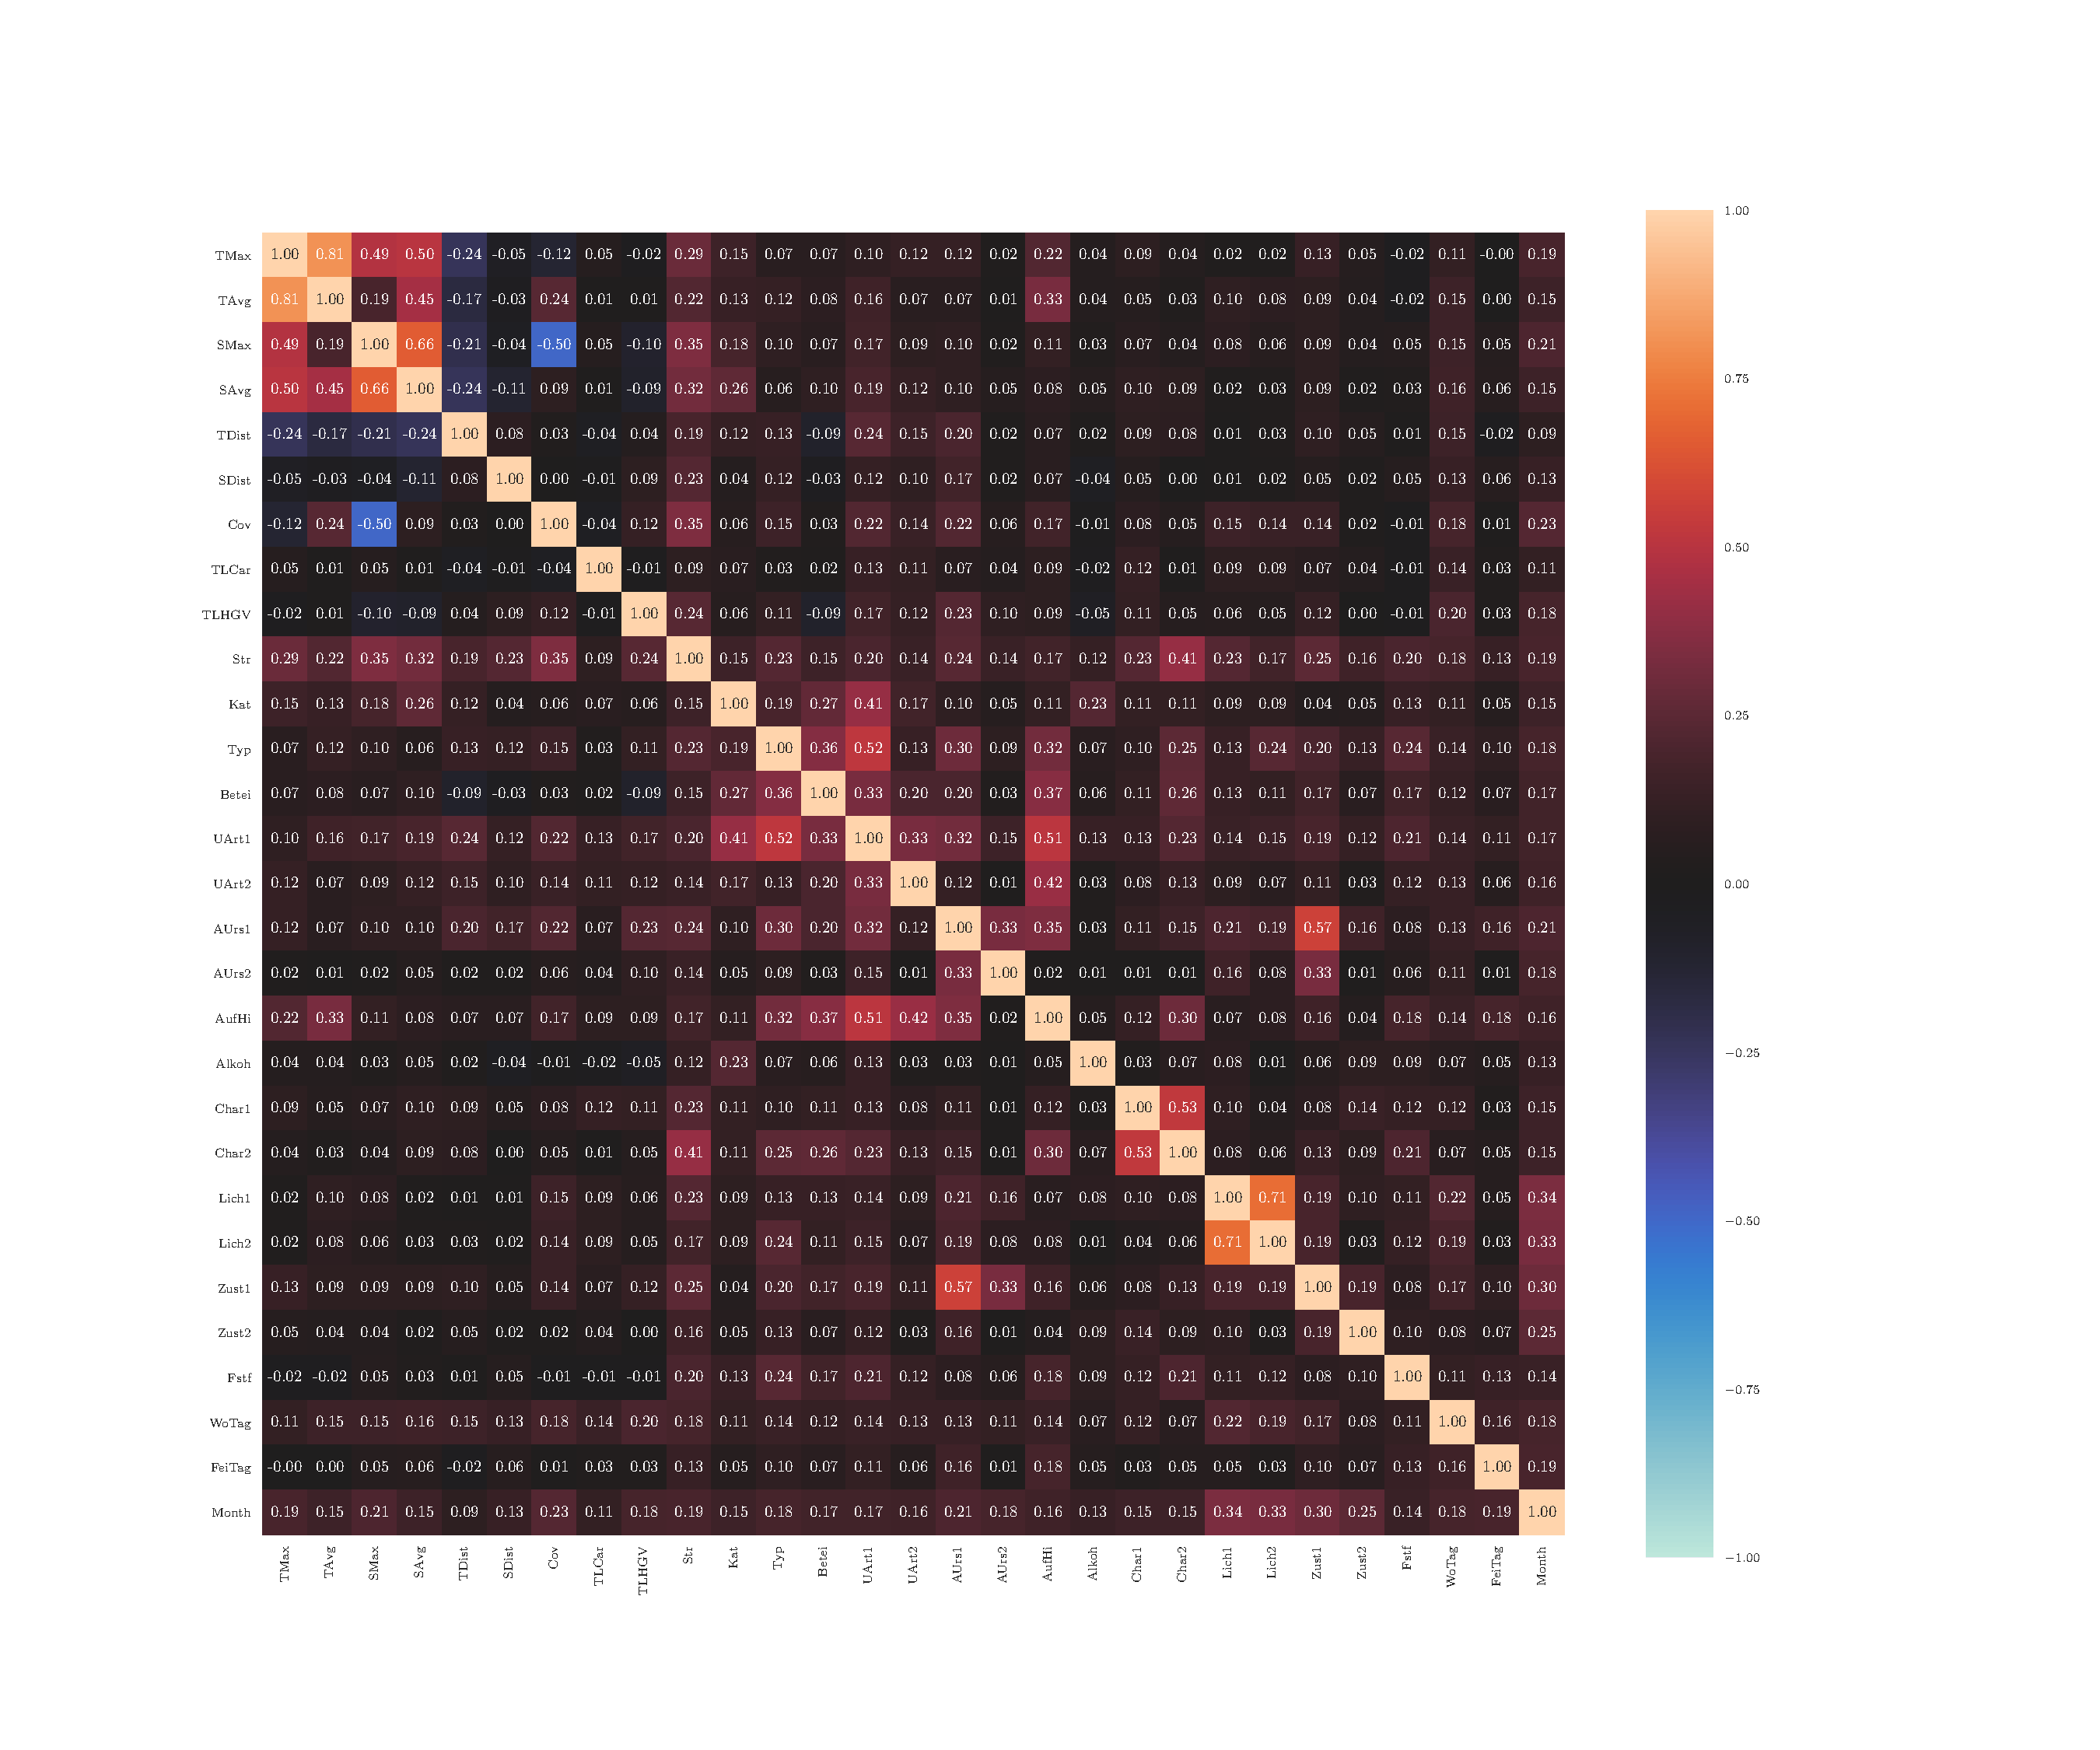
\includegraphics[width=1.4\textwidth, trim=0cm 2.5cm 6cm 3cm]{CorrAnalysis/data/BAYSIS/03_selected_03_endJam/plots/baysis_selected_corr_cramers}%
	}
	\caption{Correlation matrix for congestion-accident matched data classified as \textit{Jam Effector}, with $V$, $\eta$, $\tau$, $r_{pq}$, $r$}
	\label{img:correlation_matrix_selected_effector_cramers}
\end{figure}

% --------------------------
% -------- Strasse ---------
% --------------------------
\centerheading{Strasse}
All relations of \textit{Strasse} - \textit{TMax}, \textit{Strasse} - \textit{TAvg}, \textit{Strasse} - \textit{SMax}, \textit{Strasse} - \textit{SAvg}, \textit{Strasse} - \textit{TDist}, \textit{Strasse} - \textit{SDist}, \textit{Strasse} - \textit{Cov} and \textit{Strasse} - \textit{TLHGV} produce a $p$-value above the $\alpha$-level. The null hypothesizes can't be rejected and there are \textit{no} significant differences between the groups of \textit{Strasse} in these relations.

% ----------------------
% -------- Kat ---------
% ----------------------
\centerheading{Kat}
Both relations of \textit{Kat} - \textit{TMax} and \textit{Kat} - \textit{SAvg} produce a $p$-value above the $\alpha$-level. The null hypothesizes can't be rejected and there are \textit{no} significant differences between the groups of \textit{Kat} in these relations.

% ------------------------
% -------- UArt ---------
% ------------------------
\centerheading{UArt}
All relations of \textit{UArt1} - \textit{TAvg}, \textit{UArt1} - \textit{SAvg}, \textit{UArt1} - \textit{TDist}, \textit{UArt1} - \textit{Cov}, \textit{UArt1} - \textit{TLHGV} and \textit{UArt2} - \textit{TDist} produce a $p$-value above the $\alpha$-level. The null hypothesizes can't be rejected and there are \textit{no} significant differences between the groups of \textit{Strasse} in these relations.

% ------------------------
% -------- AUrs ---------
% ------------------------
\centerheading{AUrs}
This section analyzes the correlated relations of the accident variable \textit{AUrs1}. The correlations of \textit{AUrs1} - \textit{TDist} and \textit{AUrs1} - \textit{TLHGV} produces a $p$-value above the $\alpha$-level of .05 in the Kruskal-Wallis rank sum test. The null hypothesis can't therefore be rejected for these relations and there are no significant groups to identify.

The Kruskal-Wallis rank sum test of \textit{AUrs1} - \textit{SDist} produces a $p$-value of 0.0372, which is below $\alpha=.05$. The null hypothesis can therefore be rejected, which means there is a significant difference between the groups of \textit{Strasse}. To identify the significant groups, a pairwise Wilcoxon $T$-test for \textit{AUrs1} - \textit{TMax} is run, which produces \cref{tbl:wilcoxon_baysis_follower_AUrs1_SDist}. 
\begin{table}[ht]
	\tiny
	\centering
	\begin{tabular}{rrrrrrr}
		\toprule
		& 0 & 72 & 73 & 80 & 82 & 88 \\ 
		\midrule
		72 & 1.00 &  &  &  &  &  \\ 
		73 & 0.10 & 0.35 &  &  &  &  \\ 
		80 & 1.00 &  & 1.00 &  &  &  \\ 
		82 & 1.00 &  & 1.00 &  &  &  \\ 
		88 & 0.40 & 0.04 & 1.00 & 1.00 & 0.55 &  \\ 
		89 & 1.00 &  & 1.00 &  &  & 1.00 \\ 
		\bottomrule
	  \end{tabular}
    \caption{Pairwise Wilcoxon $T$-test for \textit{AUrs1} and \textit{Spatial Distance} (Jam Follower)}
    \label{tbl:wilcoxon_baysis_follower_AUrs1_SDist}
\end{table}
The tables shows that the differences are not group specific, since no groups differs significantly. \todo{Add section of Global and Specific Signifcancy}

The Kruskal-Wallis rank sum test of \textit{AUrs1} - \textit{Cov} produces a $p$-value of 0.0024, which is below $\alpha=.05$. The null hypothesis can therefore be rejected, which means there is a significant difference between the groups of \textit{Strasse}. To identify the significant groups, a pairwise Wilcoxon $T$-test for \textit{AUrs1} - \textit{Cov} is run, which produces \cref{tbl:wilcoxon_baysis_follower_AUrs1_Cov}. 
\begin{table}[ht]
	\tiny
	\centering
	\begin{tabular}{rrrrrrr}
		\toprule
		& 0 & 72 & 73 & 80 & 82 & 88 \\ 
		\midrule
		72 & 0.28 &  &  &  &  &  \\ 
		73 & 1.00 & 1.00 &  &  &  &  \\ 
		80 & 1.00 & 1.00 & 1.00 &  &  &  \\ 
		82 & 1.00 & 1.00 & 1.00 & 1.00 &  &  \\ 
		88 & 0.33 & 0.79 & 0.56 & 1.00 & 1.00 &  \\ 
		89 & 1.00 & 1.00 & 1.00 & 1.00 & 1.00 & 1.00 \\ 
		\bottomrule
	  \end{tabular}
    \caption{Pairwise Wilcoxon $T$-test for \textit{AUrs1} and \textit{Coverage} (Jam Follower)}
    \label{tbl:wilcoxon_baysis_follower_AUrs1_Cov}
\end{table}
The tables shows that the differences are not group specific, since no groups differs significantly. \todo{Add section of Global and Specific Signifcancy}

% ------------------------
% -------- AufHi ---------
% ------------------------
\centerheading{AufHi}
All relations of \textit{AufHi} - \textit{TMax}, \textit{AufHi} - \textit{TAvg} and \textit{AufHi} - \textit{Cov} produce a $p$-value above the $\alpha$-level. The null hypothesizes can't be rejected and there are no significant differences between the groups of \textit{AufHi} in these relations.

% ------------------------
% -------- Lich1 ---------
% ------------------------
\centerheading{Lich}
The relation of \textit{Lich1} - \textit{Cov} produce a $p$-value above $\alpha=.05$ in the Kruskal-Wallis rank sum test. The null hypothesizes can't be rejected and there are \textit{no} significant differences between the groups of \textit{Lich1}.

% ------------------------
% -------- WoTag ---------
% ------------------------
\centerheading{WoTag}

\paragraph{Maximal temporal Extent:}
Kruskal-Wallis chi-squared = 168.61, df = 167, p-value = 0.4506

\paragraph{Maximal spatial Extent:}
Kruskal-Wallis chi-squared = 448.61, df = 425, p-value = 0.2067

\paragraph{Average spatial Extent:}
Kruskal-Wallis chi-squared = 460.72, df = 433, p-value = 0.1723

\paragraph{Temporal Distance}
Kruskal-Wallis chi-squared = 22.628, df = 24, p-value = 0.5418

\paragraph{Coverage}
Kruskal-Wallis chi-squared = 73.906, df = 77, p-value = 0.5788

\paragraph{Time-loss HGV}
Kruskal-Wallis chi-squared = 318.99, df = 293, p-value = 0.1422

% ------------------------
% -------- Month ---------
% ------------------------
\centerheading{Month}

\paragraph{Maximal temporal Extent:}
Kruskal-Wallis chi-squared = 165.89, df = 168, p-value = 0.5316

\paragraph{Average temporal Extent:}
Kruskal-Wallis chi-squared = 182.94, df = 173, p-value = 0.2877

\paragraph{Maximal spatial Extent:}
Kruskal-Wallis chi-squared = 460.69, df = 427, p-value = 0.1258

\paragraph{Coverage}
Kruskal-Wallis chi-squared = 70.545, df = 77, p-value = 0.6849

\paragraph{Time-loss HGV}
Kruskal-Wallis chi-squared = 293.39, df = 293, p-value = 0.4826
\clearpage

% ------------------------
% -------- ArbIS ---------
% ------------------------
% Global
\subsection{ArbIS}
\label{analysis_processing_correlation_arbis_matched}
As with the congestion - accident datasets in \cref{analysis_processing_correlation_baysis_matched,analysis_processing_correlation_baysis_initiator,analysis_processing_correlation_baysis_effector,analysis_processing_correlation_baysis_follower} the congestion - roadwork dataset also needs to be analyzed for correlations. The correlation matrix table for the congestion-roadwork dataset (see \cref{tbl:appendix_arbis_correlation_matrix_dataset_cramers}) is visual presented in \cref{img:correlation_matrix_arbis_selected_effector_cramers} showing the the correlation of each variable combination. When visual analyzing \cref{img:correlation_matrix_arbis_selected_effector_cramers} and checking the guidelines for a strong correlation in reference to the applied coefficient (identifiable with \cref{table:appendix_coefficient_matrix_matched}) we get a list of strongly correlated variable combinations (see \cref{tbl:correlation_list_arbis_matched}). Since the focus of the thesis are the correlations between accidents and jams, these are only collected from the bottom-left rectangle of the matrix, where the congestion and accidents variables intersect. Correlations of the kind congestion - congestion or roadwork - roadwork are not considered.
\begin{table}[h!]
	\centering
	\begin{tabular}{c|l|l}  
		Category & Strong \\
		\\[-1em]
		\hline
		\\[-1em]
		Strasse & TMax, TAvg, SMax, SAvg, TDist, SDist, Cov, TLCar, TLHGV \\ 
 		%AnzGesperrtFs & & \\ 
 		%Einzug & & \\
 		%Richtung & & \\
 		%Length & & \\
 		%Duration & & \\
 		Month & TAvg, SMax, SAvg, TDist, SDist, Cov, TLCar \\
	\end{tabular}
  \caption{List of incident variables and their strong/moderated correlated jam variable from the ArbIS matched data}
  \label{tbl:correlation_list_arbis_matched}
\end{table}
As \cref{tbl:correlation_list_arbis_matched} show, only the variables Strasse and Month are correlated with congestion characteristics. Both variables tend to bias an interpretation of congestion characteristics because the 


Next we need to verify that the correlation is significant and what the correlation predicates. Therefore each correlation will be evaluated with the Post Hoc test, defined in \cref{correlation_posthoc}. In the following sections, the correlated relations of the variables in \cref{tbl:correlation_list_arbis_matched} are analyzed and an initial interpretation of each significant correlation is introduced. Groups with an insufficient sample size (see \cref{correlation_uncertainty} are neglected and not shown. The descriptive tables, showing the count ($n$), mean ($\bar{x}$), standard deviation ($\sigma$), median ($\tilde{x}$), $min$, $max$ and range ($\Delta$) therefore only contain groups with significant sample sizes.
\begin{figure}[!ht]
	\centering
	\makebox[\textwidth][c]{%
		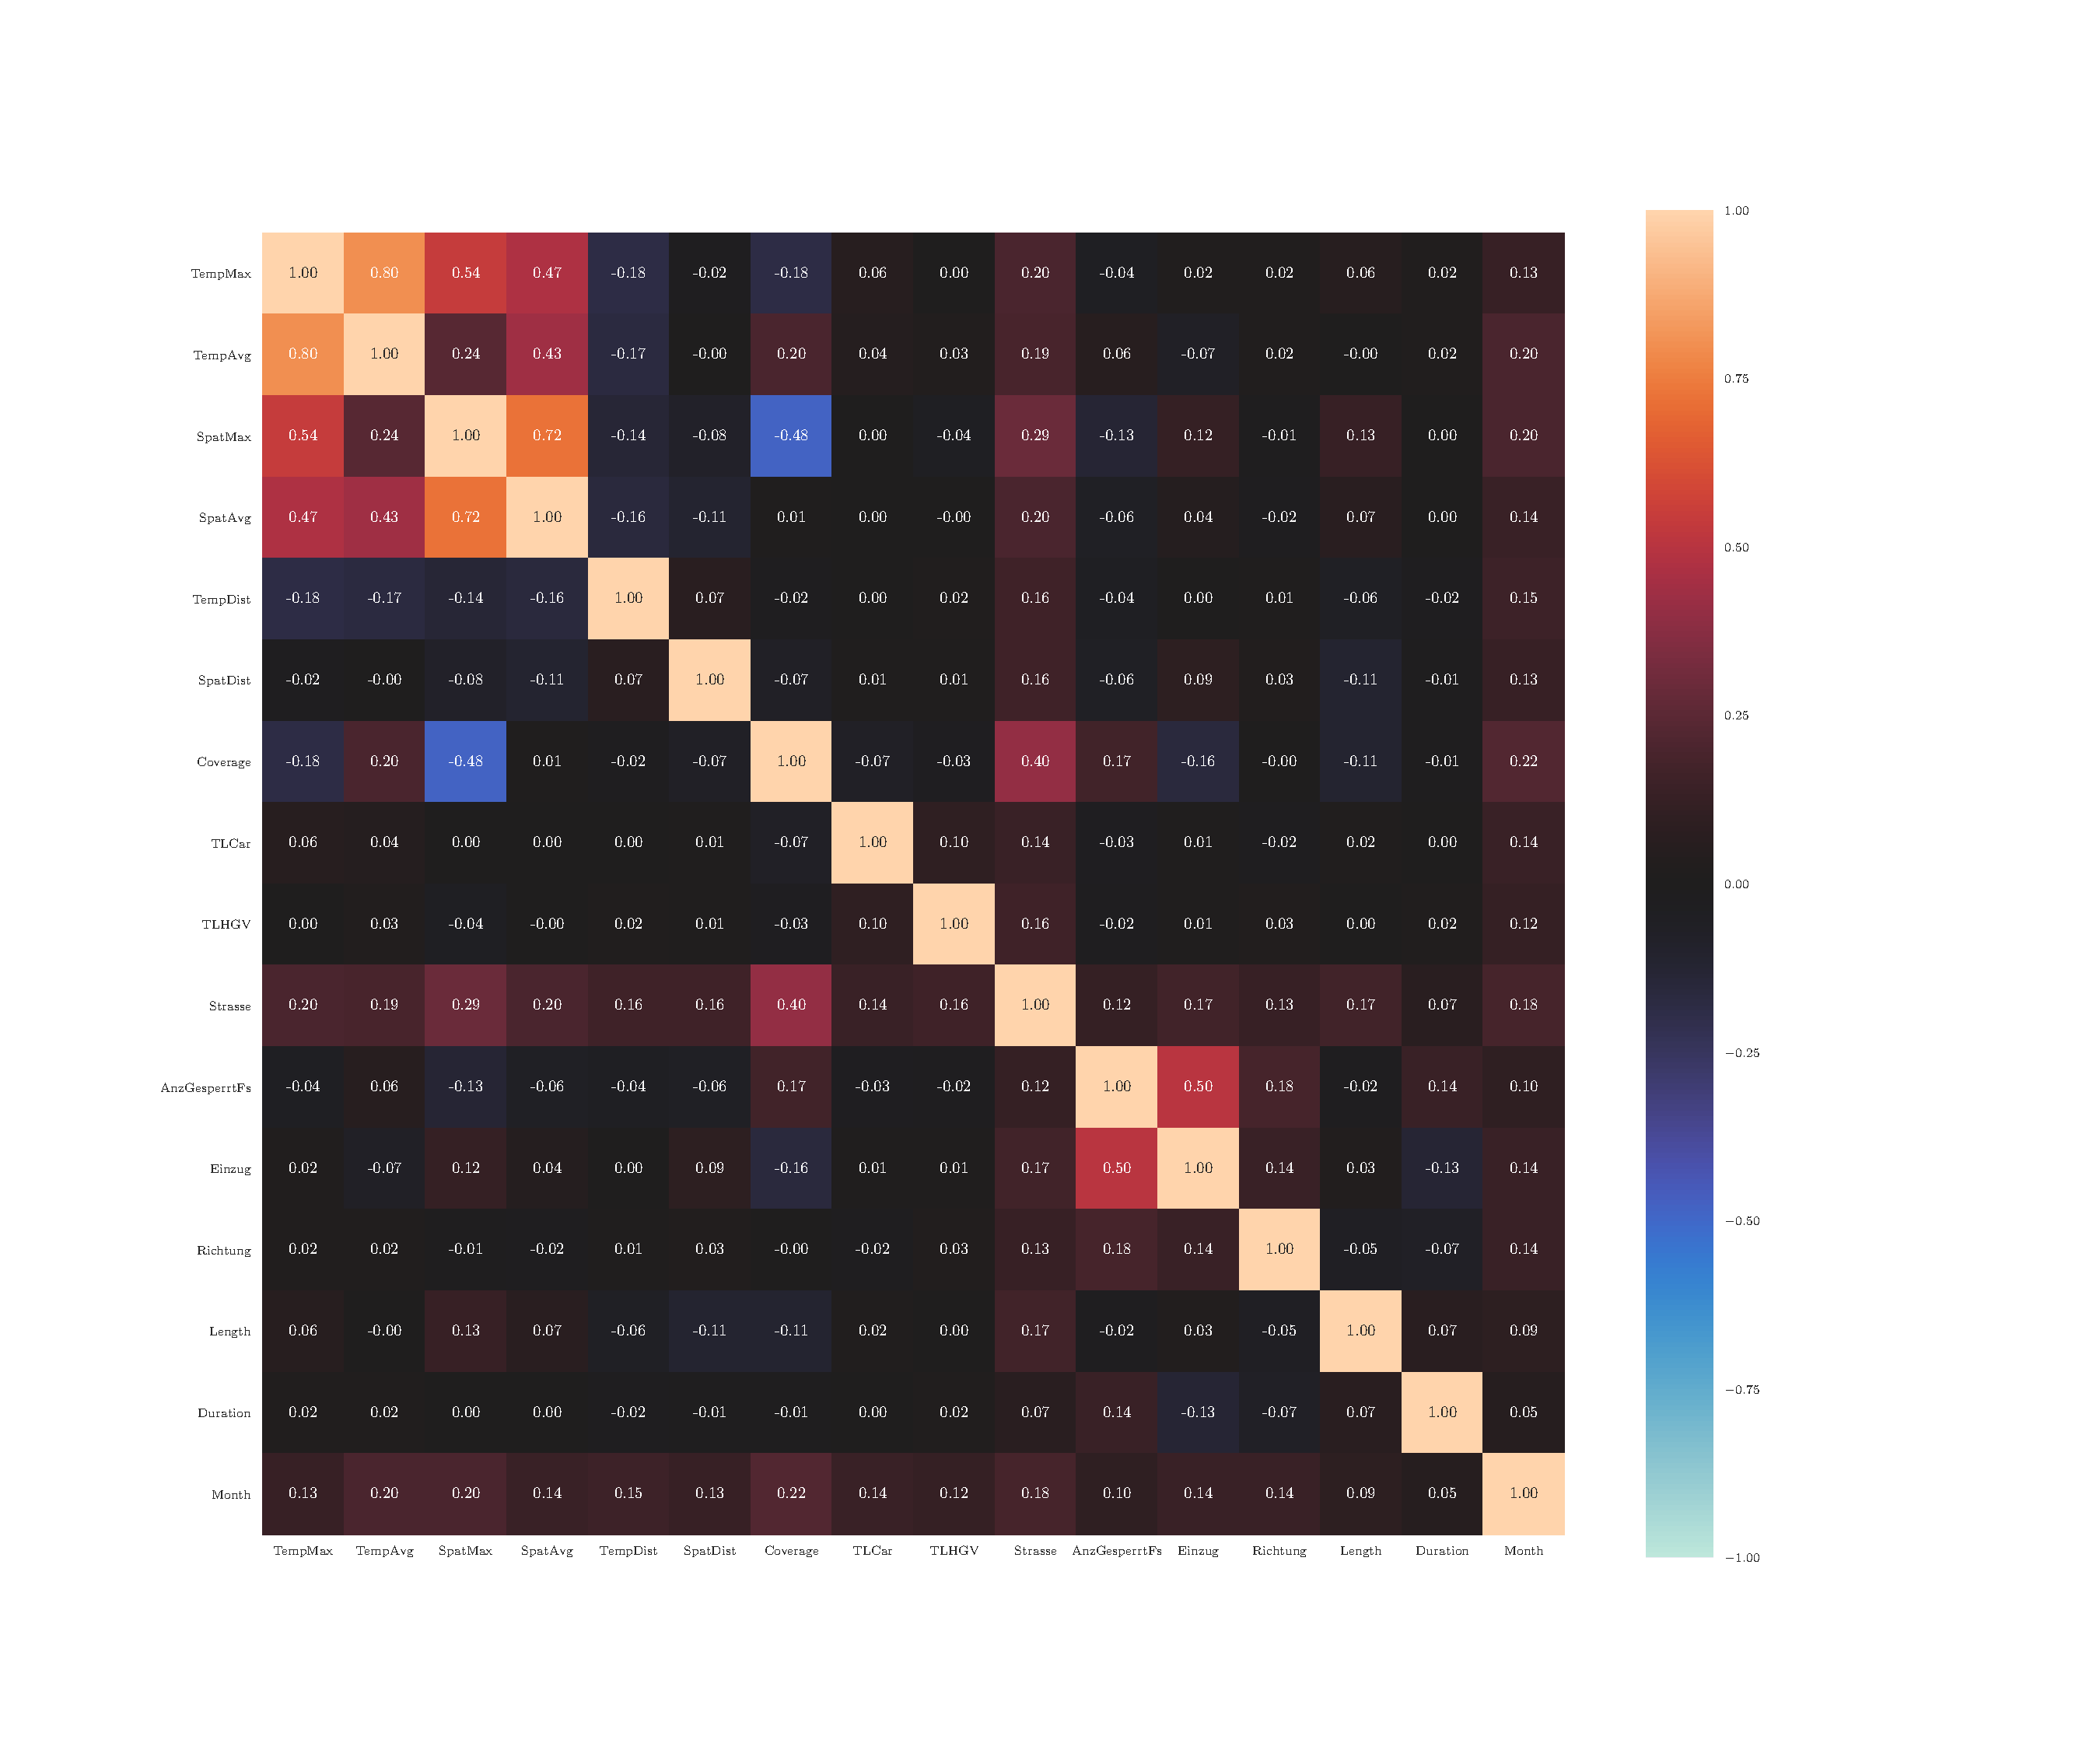
\includegraphics[width=1.4\textwidth, trim=0cm 2.5cm 6cm 3cm]{CorrAnalysis/data/ArbIS/02_matched/plots/arbis_matched_corr_cramers}%
	}
	\caption{Correlation matrix for congestion-roadwork matched data, calculated with $V$, $\eta$, $\tau$, $r_{pq}$, $r$}
	\label{img:correlation_matrix_arbis_selected_effector_cramers}
\end{figure}

% % --------------------------
% % -------- Strasse ---------
% % --------------------------
\centerheading{Strasse}
This section analyzes the correlated relations of the accident variable \textit{Strasse}. The Kruskal-Wallis rank sum test of \textit{Strasse} - \textit{TMax} produces a $p$-value of < 0.0001, which is below $\alpha$. The null hypothesis can therefore be rejected, which means there is a significant difference between the groups of \textit{Strasse}. To identify the significant groups, a pairwise Wilcoxon $T$-test for \textit{Strasse} - \textit{TMax} is run, which produces \cref{tbl:wilcoxon_arbis_matched_Strasse_TMax}. 
\begin{table}[ht!]
	\tiny
	\centering
    \begin{tabular}{rrrrrrrrrrrrrrrrr}
		\toprule
			& A9 & A7 & A70 & A71 & A6 & A73 & A3 & A99 & A96 & A995 & A92 & A72 & A93 & A95 & A94 & A980 \\ 
		\midrule
		% A7   & 1.00 &  &  &  &  &  &  &  &  &  &  &  &  &  &  &  \\ 
		% A70  & 1.00 & 1.00 &  &  &  &  &  &  &  &  &  &  &  &  &  &  \\ 
		% A71  & 1.00 & 1.00 & 1.00 &  &  &  &  &  &  &  &  &  &  &  &  &  \\ 
		% A6   & 1.00 & 1.00 & 1.00 & 1.00 &  &  &  &  &  &  &  &  &  &  &  &  \\ 
		% A73  & 1.00 & 1.00 & 1.00 & 1.00 & 1.00 &  &  &  &  &  &  &  &  &  &  &  \\ 
		A3   & \red{0.00} & \red{0.04} & 1.00 & 1.00 & \red{0.01} & 1.00 &  &  &  &  &  &  &  &  &  &  \\ 
		% A99  & 1.00 & 1.00 & 1.00 & 1.00 & 0.48 & 1.00 & 1.00 &  &  &  &  &  &  &  &  &  \\ 
		A96  & 1.00 & 0.82 & 1.00 & 1.00 & 1.00 & 1.00 & \red{0.00} & \red{0.00} &  &  &  &  &  &  &  &  \\ 
		% A995 & 1.00 & 1.00 & 1.00 & 1.00 & 1.00 & 1.00 & 0.79 & 0.74 & 1.00 &  &  &  &  &  &  &  \\ 
		% A92  & 1.00 & 1.00 & 1.00 & 1.00 & 1.00 & 1.00 & 1.00 & 1.00 & 1.00 & 1.00 &  &  &  &  &  &  \\ 
		% A72  & 1.00 & 1.00 & 1.00 & 1.00 & 1.00 & 1.00 & 1.00 & 1.00 & 1.00 & 1.00 & 1.00 &  &  &  &  &  \\ 
		A93  & \red{0.00} & \red{0.00} & 1.00 & 0.09 & \red{0.00} & \red{0.00} & 1.00 & 1.00 & \red{0.00} & \red{0.00} & \red{0.00} & 1.00 &  &  &  &  \\ 
		% A95  & 1.00 & 1.00 & 1.00 & 1.00 & 1.00 & 1.00 & 1.00 & 1.00 & 1.00 & 1.00 & 1.00 & 1.00 & 1.00 &  &  &  \\ 
		A94  & 1.00 & 1.00 & 1.00 & 1.00 & 0.68 & 1.00 & 1.00 & 1.00 & \red{0.01} & 0.48 & 1.00 & 1.00 & 1.00 & 1.00 &  &  \\ 
		% A980 & 1.00 & 1.00 & 1.00 & 1.00 & 1.00 & 1.00 & 1.00 & 1.00 & 1.00 & 1.00 & 1.00 & 1.00 & 1.00 & 1.00 & 1.00 &  \\ 
		% A45  & 1.00 & 1.00 & 1.00 & 1.00 & 1.00 & 1.00 & 1.00 & 1.00 & 1.00 & 1.00 & 1.00 & 1.00 & 1.00 & 1.00 & 1.00 & 1.00 \\ 
		\bottomrule
	\end{tabular}
	\caption{Pairwise Wilcoxon $T$-test for \textit{Strasse} and \textit{Maximal Temporal Extent}}
	\label{tbl:wilcoxon_arbis_matched_Strasse_TMax}
\end{table}
The table shows, that the groups A3 and A93 differ from group A9, A7 and A6. The A93 also differs from A96, A995 and A92. The A96 differs from A3 and A99.
\begin{table}[ht!]
	\tiny
	\centering
  \begin{tabular}{rrrrrrrrrrrrrr}
    \toprule
    Group & $n$ & $\bar{x}$ & $\sigma$ & $\tilde{x}$ & $min$ & $max$ & $\Delta$ \\
    \midrule
    A9   & 656  & 159.55 & 175.78 & 100.50 & 9   & 1323 & 1314 \\ 
    A7   & 302  & 158.38 & 213.55 & 87.00  & 9   & 1323 & 1314 \\ 
    A70  & 50   & 228.90 & 279.03 & 105.00 & 15  & 963  & 948 \\ 
    A71  & 10   & 83.40  & 72.87  & 48.00  & 36  & 249  & 213 \\ 
    A6   & 198  & 142.24 & 166.46 & 85.50  & 9   & 864  & 855 \\ 
    A73  & 86   & 153.59 & 235.85 & 100.50 & 9   & 1323 & 1314 \\ 
    A3   & 1023 & 233.66 & 279.35 & 123.00 & 9   & 1326 & 1317 \\ 
    A99  & 312  & 158.88 & 155.05 & 135.00 & 9   & 1320 & 1311 \\ 
    A96  & 230  & 105.80 & 95.17  & 75.00  & 9   & 384  & 375 \\ 
    A995 & 14   & 60.00  & 28.70  & 48.00  & 18  & 105  & 87 \\ 
    A92  & 82   & 132.40 & 134.72 & 79.50  & 9   & 768  & 759 \\ 
    A93  & 160  & 157.33 & 55.97  & 189.00 & 9   & 312  & 303 \\  
    A94  & 56   & 179.57 & 124.79 & 165.00 & 15  & 369  & 354 \\ 
    \bottomrule
  \end{tabular}
	\caption{Group descriptives of \textit{Strasse} and \textit{Maximal Temporal Extent}}
	\label{tbl:descriptives_arbis_matched_Strasse_TMax}
	%\vspace{-8mm}
\end{table}
With the descriptives in \cref{tbl:descriptives_arbis_matched_Strasse_TMax} and the named significant differences it can be interpreted that roadworks on the A3 result in 80\,\% longer $\bar{x}$ than on the A9, A7 and A6. The A70 has a similar difference. Roadworks on the A96 and A995 result in significantly shorter $\bar{x}$ than on the A3 and A99.

The Kruskal-Wallis rank sum test of \textit{Strasse} - \textit{TAvg} produces a $p$-value of < 0.0001, which is below $\alpha$. The null hypothesis can therefore be rejected, which means there is a significant difference between the groups of \textit{Strasse}. To identify the significant groups, a pairwise Wilcoxon $T$-test for \textit{Strasse} - \textit{TAvg} is run, which produces \cref{tbl:wilcoxon_arbis_matched_Strasse_TAvg}. 
\begin{table}[ht!]
	\tiny
	\setlength{\tabcolsep}{4pt}
	\centering
  \begin{tabular}{rrrrrrrrrrrrrrrrr}
    \toprule
         & A9 & A7 & A70 & A71 & A6 & A73 & A3 & A99 & A96 & A995 & A92 & A72 & A93 & A95 & A94 & A980 \\ 
    \midrule
    A7   & 1.00 &  &  &  &  &  &  &  &  &  &  &  &  &  &  &  \\ 
    A70  & 1.00 & 1.00 &  &  &  &  &  &  &  &  &  &  &  &  &  &  \\ 
    A71  & 1.00 & 1.00 & 1.00 &  &  &  &  &  &  &  &  &  &  &  &  &  \\ 
    A6   & 1.00 & 1.00 & 1.00 & 1.00 &  &  &  &  &  &  &  &  &  &  &  &  \\ 
    A73  & 1.00 & 1.00 & 1.00 & 1.00 & 1.00 &  &  &  &  &  &  &  &  &  &  &  \\ 
    A3   & 1.00 & 1.00 & 1.00 & 1.00 & 0.69 & 1.00 &  &  &  &  &  &  &  &  &  &  \\ 
    A99  & \red{0.00} & \red{0.00} & 0.08 & 1.00 & 1.00 & 1.00 & \red{0.00} &  &  &  &  &  &  &  &  &  \\ 
    A96  & 1.00 & 1.00 & 1.00 & 1.00 & 1.00 & 1.00 & 1.00 & 0.55 &  &  &  &  &  &  &  &  \\ 
    A995 & 1.00 & 1.00 & 1.00 & 1.00 & 1.00 & 1.00 & 1.00 & 1.00 & 1.00 &  &  &  &  &  &  &  \\ 
    A92  & 1.00 & 1.00 & 1.00 & 1.00 & 1.00 & 1.00 & 1.00 & \red{0.04} & 1.00 & 1.00 &  &  &  &  &  &  \\ 
    A72  & 1.00 & 1.00 & 1.00 & 1.00 & 1.00 & 1.00 & 1.00 & 1.00 & 1.00 & 1.00 & 1.00 &  &  &  &  &  \\ 
    A93  & \red{0.00} & \red{0.00} & 1.00 & 0.24 & \red{0.00} & \red{0.00} & \red{0.00} & \red{0.00} & \red{0.00} & \red{0.00} & \red{0.00} & 1.00 &  &  &  &  \\ 
    A95  & 1.00 & 1.00 & 1.00 & 1.00 & 1.00 & 1.00 & 1.00 & 1.00 & 1.00 & 1.00 & 1.00 & 1.00 & 1.00 &  &  &  \\ 
    A94  & 1.00 & 1.00 & 1.00 & 1.00 & 0.14 & 1.00 & 1.00 & 0.00 & 0.63 & 0.53 & 1.00 & 1.00 & 0.02 & 1.00 &  &  \\ 
    A980 & 1.00 & 1.00 & 1.00 & 1.00 & 1.00 & 1.00 & 1.00 & 1.00 & 1.00 & 1.00 & 1.00 & 1.00 & 1.00 & 1.00 & 1.00 &  \\ 
    A45  & 1.00 & 1.00 & 1.00 & 1.00 & 1.00 & 1.00 & 1.00 & 1.00 & 1.00 & 1.00 & 1.00 & 1.00 & 1.00 & 1.00 & 1.00 & 1.00 \\ 
    \midrule
  \end{tabular}
	\caption{Pairwise Wilcoxon $T$-test for \textit{Strasse} and \textit{Average Temporal Extent}}
	\label{tbl:wilcoxon_arbis_matched_Strasse_TAvg}
\end{table}
The table shows, that the groups A99 and A93 differ from group A9 and A7. The A93 also differs from the A6, A73, A3, A99, A96, A995 and A92. The A92 differs from A99.
\begin{table}[ht!]
	\tiny
	\centering
  \begin{tabular}{rrrrrrrrrrrrrr}
    \toprule
    Group & $n$ & $\bar{x}$ & $\sigma$ & $\tilde{x}$ & $min$ & $max$ & $\Delta$ \\
    \midrule
    A9   & 656  & 85.61  & 100.78 & 42.00  & 5  & 575  & 570 \\ 
    A7   & 302  & 87.76  & 117.13 & 44.50  & 5  & 858  & 853 \\ 
    A70  & 50   & 154.38 & 236.49 & 55.50  & 6  & 966  & 960 \\ 
    A71  & 10   & 64.90  & 71.81  & 38.00  & 18 & 252  & 234 \\ 
    A6   & 198  & 65.60  & 86.36  & 41.00  & 4  & 630  & 626 \\ 
    A73  & 86   & 56.23  & 45.35  & 42.50  & 6  & 190  & 184 \\ 
    A3   & 1023 & 89.94  & 124.69 & 51.00  & 3  & 1326 & 1323 \\ 
    A99  & 312  & 45.38  & 41.73  & 33.00  & 3  & 291  & 288 \\ 
    A96  & 230  & 69.31  & 73.52  & 43.00  & 5  & 290  & 285 \\ 
    A995 & 14   & 37.14  & 23.98  & 23.00  & 8  & 74   & 66 \\ 
    A92  & 82   & 81.83  & 90.35  & 45.50  & 5  & 489  & 484 \\ 
    A93  & 160  & 115.96 & 50.96  & 141.00 & 6  & 199  & 193 \\ 
    A94  & 56   & 84.98  & 64.07  & 70.00  & 6  & 248  & 242 \\ 
    \midrule
  \end{tabular}
	\caption{Group descriptives of \textit{Strasse} and \textit{Average Temporal Extent}}
	\label{tbl:descriptives_arbis_matched_Strasse_TAvg}
	%\vspace{-8mm}
\end{table}
With the descriptives in \cref{tbl:descriptives_arbis_matched_Strasse_TAvg} it can be interpreted that roadworks on the A93 result in sing

The Kruskal-Wallis rank sum test of \textit{Strasse} - \textit{SMax} produces a $p$-value of < 0.0001, which is below $\alpha$. The null hypothesis can therefore be rejected, which means there is a significant difference between the groups of \textit{Strasse}. To identify the significant groups, a pairwise Wilcoxon $T$-test for \textit{Strasse} - \textit{SMax} is run, which produces \cref{tbl:wilcoxon_arbis_matched_Strasse_SMax}. 
\begin{table}[ht!]
	\tiny
	\setlength{\tabcolsep}{4pt}
	\centering
  \begin{tabular}{rrrrrrrrrrrrrrrrr}
    \toprule
         & A9 & A7 & A70 & A71 & A6 & A73 & A3 & A99 & A96 & A995 & A92 & A72 & A93 & A95 & A94 & A980 \\ 
    \hline
    A7   & 0.58 &  &  &  &  &  &  &  &  &  &  &  &  &  &  &  \\ 
    A70  & 1.00 & 1.00 &  &  &  &  &  &  &  &  &  &  &  &  &  &  \\ 
    A71  & 1.00 & 1.00 & 1.00 &  &  &  &  &  &  &  &  &  &  &  &  &  \\ 
    A6   & 1.00 & 1.00 & 1.00 & 1.00 &  &  &  &  &  &  &  &  &  &  &  &  \\ 
    A73  & 1.00 & 1.00 & 1.00 & 1.00 & 1.00 &  &  &  &  &  &  &  &  &  &  &  \\ 
    A3   & 0.00 & 0.00 & 0.00 & 0.52 & 0.01 & 0.05 &  &  &  &  &  &  &  &  &  &  \\ 
    A99  & 0.07 & 0.00 & 0.01 & 0.21 & 0.26 & 0.20 & 1.00 &  &  &  &  &  &  &  &  &  \\ 
    A96  & 0.00 & 0.06 & 1.00 & 1.00 & 0.00 & 1.00 & 0.00 & 0.00 &  &  &  &  &  &  &  &  \\ 
    A995 & 1.00 & 1.00 & 1.00 & 1.00 & 1.00 & 1.00 & 0.11 & 0.03 & 1.00 &  &  &  &  &  &  &  \\ 
    A92  & 1.00 & 1.00 & 1.00 & 1.00 & 1.00 & 1.00 & 0.00 & 0.00 & 0.04 & 1.00 &  &  &  &  &  &  \\ 
    A72  & 1.00 & 1.00 & 1.00 & 1.00 & 1.00 & 1.00 & 1.00 & 1.00 & 1.00 & 0.81 & 1.00 &  &  &  &  &  \\ 
    A93  & 0.00 & 0.00 & 0.02 & 1.00 & 0.00 & 0.00 & 0.00 & 0.00 & 0.00 & 1.00 & 0.00 & 0.73 &  &  &  &  \\ 
    A95  & 1.00 & 1.00 & 1.00 & 1.00 & 1.00 & 1.00 & 1.00 & 1.00 & 1.00 & 1.00 & 1.00 & 1.00 & 1.00 &  &  &  \\ 
    A94  & 1.00 & 1.00 & 1.00 & 1.00 & 1.00 & 1.00 & 0.04 & 0.04 & 0.89 & 1.00 & 1.00 & 1.00 & 0.00 & 1.00 &  &  \\ 
    A980 & 1.00 & 1.00 & 1.00 & 1.00 & 1.00 & 1.00 & 1.00 & 1.00 & 1.00 & 1.00 & 1.00 & 1.00 & 1.00 & 1.00 & 1.00 &  \\ 
    A45  & 1.00 & 1.00 & 1.00 & 1.00 & 1.00 & 1.00 & 1.00 & 1.00 & 1.00 & 1.00 & 1.00 & 1.00 & 1.00 & 1.00 & 1.00 & 1.00 \\ 
    \hline
  \end{tabular}
	\caption{Pairwise Wilcoxon $T$-test for \textit{Strasse} and \textit{Maximal Spatial Extent}}
	\label{tbl:wilcoxon_arbis_matched_Strasse_SMax}
\end{table}
\cref{tbl:wilcoxon_arbis_matched_Strasse_SMax} shows, that the groups A6, A9, A7, A70, A73, A92, A94 and A96 differ from group A3. There is no distinctive general trend.
\begin{table}[ht!]
	\tiny
	\centering
  \begin{tabular}{rrrrrrrrrrrrrr}
    \hline
    & vars & n & mean & sd & median & trimmed & mad & min & max & range & skew & kurtosis & se \\ 
    \hline
    A9   & 1.00 & 656.00 & 8655.57 & 8521.51 & 4778.00 & 6972.99 & 3783.60 & 1035.00 & 49765.00 & 48730.00 & 1.85 & 3.49 & 332.71 \\ 
    A7   & 1.00 & 302.00 & 6238.63 & 4902.30 & 4397.00 & 5486.83 & 2874.76 & 902.00 & 20030.00 & 19128.00 & 1.21 & 0.37 & 282.10 \\ 
    A70  & 1.00 & 50.00 & 5729.56 & 4763.20 & 3224.00 & 4856.50 & 2511.52 & 1365.00 & 20249.00 & 18884.00 & 1.39 & 1.03 & 673.62 \\ 
    A71  & 1.00 & 10.00 & 3899.00 & 2746.84 & 2339.00 & 3336.25 & 391.41 & 2075.00 & 10225.00 & 8150.00 & 1.20 & 0.06 & 868.63 \\ 
    A6   & 1.00 & 198.00 & 8421.67 & 8209.85 & 5690.00 & 6919.39 & 4487.83 & 965.00 & 40033.00 & 39068.00 & 1.83 & 3.14 & 583.45 \\ 
    A73  & 1.00 & 86.00 & 7717.21 & 7747.18 & 4813.00 & 6183.17 & 4233.56 & 1095.00 & 33764.00 & 32669.00 & 1.99 & 3.84 & 835.40 \\ 
    A3   & 1.00 & 1023.00 & 11836.50 & 11045.29 & 7979.00 & 9944.23 & 7856.30 & 1014.00 & 47607.00 & 46593.00 & 1.40 & 1.38 & 345.33 \\ 
    A99  & 1.00 & 312.00 & 9337.49 & 7230.99 & 7978.00 & 8264.88 & 6980.82 & 991.00 & 48987.00 & 47996.00 & 1.78 & 4.68 & 409.37 \\ 
    A96  & 1.00 & 230.00 & 5639.41 & 6034.92 & 3072.00 & 4226.37 & 1856.96 & 951.00 & 27965.00 & 27014.00 & 2.07 & 3.48 & 397.93 \\ 
    A995 & 1.00 & 14.00 & 3618.14 & 1331.10 & 4288.00 & 3684.67 & 796.16 & 1613.00 & 4825.00 & 3212.00 & -0.35 & -1.78 & 355.75 \\ 
    A92  & 1.00 & 82.00 & 5758.10 & 3673.73 & 4544.00 & 5227.71 & 3114.94 & 999.00 & 16931.00 & 15932.00 & 1.22 & 0.92 & 405.70 \\ 
    A93  & 1.00 & 160.00 & 3530.39 & 3718.54 & 1926.00 & 2571.59 & 34.10 & 699.00 & 22528.00 & 21829.00 & 3.21 & 9.95 & 293.98 \\ 
    A94  & 1.00 & 56.00 & 5849.05 & 3394.57 & 5785.00 & 5667.57 & 2513.01 & 1025.00 & 12582.00 & 11557.00 & 0.47 & -0.67 & 453.62 \\ 
    \hline
  \end{tabular}
	\caption{Group descriptives of \textit{Strasse} and \textit{Maximal Spatial Extent}}
	\label{tbl:descriptives_arbis_matched_Strasse_SMax}
	%\vspace{-8mm}
\end{table}
The descriptives in \cref{tbl:descriptives_arbis_matched_Strasse_SMax}

The Kruskal-Wallis rank sum test of \textit{Strasse} - \textit{SAvg} produces a $p$-value of < 0.0001, which is below $\alpha$. The null hypothesis can therefore be rejected, which means there is a significant difference between the groups of \textit{Strasse}. To identify the significant groups, a pairwise Wilcoxon $T$-test for \textit{Strasse} - \textit{SAvg} is run, which produces \cref{tbl:wilcoxon_arbis_matched_Strasse_SAvg}. 
\begin{table}[ht!]
	\tiny
	\setlength{\tabcolsep}{4pt}
	\centering
  \begin{tabular}{rrrrrrrrrrrrrrrrr}
    \hline
         & A9 & A7 & A70 & A71 & A6 & A73 & A3 & A99 & A96 & A995 & A92 & A72 & A93 & A95 & A94 & A980 \\ 
    \hline
    A7   & 0.06 &  &  &  &  &  &  &  &  &  &  &  &  &  &  &  \\ 
    A70  & 1.00 & 1.00 &  &  &  &  &  &  &  &  &  &  &  &  &  &  \\ 
    A71  & 1.00 & 1.00 & 1.00 &  &  &  &  &  &  &  &  &  &  &  &  &  \\ 
    A6   & 1.00 & 1.00 & 1.00 & 1.00 &  &  &  &  &  &  &  &  &  &  &  &  \\ 
    A73  & 0.62 & 1.00 & 1.00 & 1.00 & 1.00 &  &  &  &  &  &  &  &  &  &  &  \\ 
    A3   & 1.00 & 0.00 & 1.00 & 1.00 & 1.00 & 0.02 &  &  &  &  &  &  &  &  &  &  \\ 
    A99  & 0.01 & 1.00 & 1.00 & 1.00 & 0.75 & 1.00 & 0.00 &  &  &  &  &  &  &  &  &  \\ 
    A96  & 0.00 & 1.00 & 1.00 & 1.00 & 0.44 & 1.00 & 0.00 & 1.00 &  &  &  &  &  &  &  &  \\ 
    A995 & 1.00 & 1.00 & 1.00 & 1.00 & 1.00 & 1.00 & 1.00 & 1.00 & 1.00 &  &  &  &  &  &  &  \\ 
    A92  & 1.00 & 0.62 & 1.00 & 1.00 & 1.00 & 0.73 & 1.00 & 0.10 & 0.14 & 1.00 &  &  &  &  &  &  \\ 
    A72  & 1.00 & 1.00 & 1.00 & 1.00 & 1.00 & 1.00 & 1.00 & 1.00 & 1.00 & 1.00 & 1.00 &  &  &  &  &  \\ 
    A93  & 0.00 & 0.13 & 1.00 & 1.00 & 0.00 & 1.00 & 0.00 & 0.11 & 1.00 & 1.00 & 0.00 & 1.00 &  &  &  &  \\ 
    A95  & 1.00 & 1.00 & 1.00 & 1.00 & 1.00 & 1.00 & 1.00 & 1.00 & 1.00 & 1.00 & 1.00 & 1.00 & 1.00 &  &  &  \\ 
    A94  & 1.00 & 1.00 & 1.00 & 1.00 & 1.00 & 1.00 & 1.00 & 1.00 & 1.00 & 1.00 & 1.00 & 1.00 & 1.00 & 1.00 &  &  \\ 
    A980 & 1.00 & 1.00 & 1.00 & 1.00 & 1.00 & 1.00 & 1.00 & 1.00 & 1.00 & 1.00 & 1.00 & 1.00 & 1.00 & 1.00 & 1.00 &  \\ 
    A45  & 1.00 & 1.00 & 1.00 & 1.00 & 1.00 & 1.00 & 1.00 & 1.00 & 1.00 & 1.00 & 1.00 & 1.00 & 1.00 & 1.00 & 1.00 & 1.00 \\ 
    \hline
  \end{tabular}
	\caption{Pairwise Wilcoxon $T$-test for \textit{Strasse} and \textit{Average Spatial Extent}}
	\label{tbl:wilcoxon_arbis_matched_Strasse_SAvg}
\end{table}
\cref{tbl:wilcoxon_arbis_matched_Strasse_SAvg} shows, that the groups A6, A9, A7, A70, A73, A92, A94 and A96 differ from group A3. There is no distinctive general trend.
\begin{table}[ht!]
	\tiny
	\centering
  \begin{tabular}{rrrrrrrrrrrrrr}
    \hline
    & vars & n & mean & sd & median & trimmed & mad & min & max & range & skew & kurtosis & se \\ 
    \hline
    A9   & 1.00 & 656.00 & 3537.87 & 3014.80 & 2388.50 & 2920.30 & 1381.78 & 697.00 & 14785.00 & 14088.00 & 1.76 & 2.51 & 117.71 \\ 
    A7   & 1.00 & 302.00 & 2917.97 & 2988.99 & 2113.50 & 2271.17 & 1127.52 & 284.00 & 15602.00 & 15318.00 & 3.08 & 9.64 & 172.00 \\ 
    A70  & 1.00 & 50.00 & 3170.10 & 3033.98 & 1816.00 & 2516.70 & 962.21 & 532.00 & 12543.00 & 12011.00 & 1.72 & 1.88 & 429.07 \\ 
    A71  & 1.00 & 10.00 & 2572.50 & 3027.05 & 1323.00 & 1812.25 & 690.89 & 802.00 & 10425.00 & 9623.00 & 1.73 & 1.62 & 957.24 \\ 
    A6   & 1.00 & 198.00 & 3189.79 & 2385.78 & 2267.00 & 2780.79 & 1272.07 & 458.00 & 14150.00 & 13692.00 & 1.63 & 2.60 & 169.55 \\ 
    A73  & 1.00 & 86.00 & 2508.40 & 1834.03 & 2006.00 & 2228.70 & 1316.55 & 419.00 & 10039.00 & 9620.00 & 1.86 & 4.15 & 197.77 \\ 
    A3   & 1.00 & 1023.00 & 3733.90 & 2979.43 & 2835.00 & 3227.67 & 2269.86 & 355.00 & 15054.00 & 14699.00 & 1.54 & 2.09 & 93.15 \\ 
    A99  & 1.00 & 312.00 & 2381.29 & 1265.40 & 1974.00 & 2225.76 & 1073.40 & 502.00 & 5931.00 & 5429.00 & 1.00 & 0.27 & 71.64 \\ 
    A96  & 1.00 & 230.00 & 2488.22 & 1790.94 & 2160.00 & 2144.86 & 1068.21 & 404.00 & 9767.00 & 9363.00 & 2.10 & 4.77 & 118.09 \\ 
    A995 & 1.00 & 14.00 & 1976.93 & 1044.51 & 1950.00 & 1992.67 & 1714.63 & 569.00 & 3196.00 & 2627.00 & 0.06 & -1.72 & 279.16 \\ 
    A92  & 1.00 & 82.00 & 3360.88 & 2294.30 & 2882.00 & 3040.65 & 1786.53 & 457.00 & 11703.00 & 11246.00 & 1.27 & 1.23 & 253.36 \\ 
    A93  & 1.00 & 160.00 & 2243.26 & 2065.34 & 1575.00 & 1749.74 & 449.23 & 461.00 & 11161.00 & 10700.00 & 3.42 & 11.30 & 163.28 \\  
    A94  & 1.00 & 56.00 & 2557.62 & 1655.86 & 2551.00 & 2354.04 & 1104.54 & 506.00 & 6393.00 & 5887.00 & 1.06 & 0.54 & 221.27 \\ 
    \hline
  \end{tabular}
	\caption{Group descriptives of \textit{Strasse} and \textit{Average Spatial Extent}}
	\label{tbl:descriptives_arbis_matched_Strasse_SAvg}
	%\vspace{-8mm}
\end{table}
The descriptives in \cref{tbl:descriptives_arbis_matched_Strasse_SAvg}

The Kruskal-Wallis rank sum test of \textit{Strasse} - \textit{TDist} produces a $p$-value of < 0.0001, which is below $\alpha$. The null hypothesis can therefore be rejected, which means there is a significant difference between the groups of \textit{Strasse}. To identify the significant groups, a pairwise Wilcoxon $T$-test for \textit{Strasse} - \textit{TDist} is run, which produces \cref{tbl:wilcoxon_arbis_matched_Strasse_TDist}. 
\begin{table}[ht!]
	\tiny
	\setlength{\tabcolsep}{4pt}
	\centering
  \begin{tabular}{rrrrrrrrrrrrrrrrr}
    \hline
         & A9 & A7 & A70 & A71 & A6 & A73 & A3 & A99 & A96 & A995 & A92 & A72 & A93 & A95 & A94 & A980 \\ 
    \hline
    A7   & 0.00 &  &  &  &  &  &  &  &  &  &  &  &  &  &  &  \\ 
    A70  & 0.57 & 1.00 &  &  &  &  &  &  &  &  &  &  &  &  &  &  \\ 
    A71  & 1.00 & 1.00 & 1.00 &  &  &  &  &  &  &  &  &  &  &  &  &  \\ 
    A6   & 0.10 & 1.00 & 1.00 & 1.00 &  &  &  &  &  &  &  &  &  &  &  &  \\ 
    A73  & 1.00 & 1.00 & 1.00 & 1.00 & 1.00 &  &  &  &  &  &  &  &  &  &  &  \\ 
    A3   & 0.00 & 1.00 & 1.00 & 1.00 & 1.00 & 0.85 &  &  &  &  &  &  &  &  &  &  \\ 
    A99  & 0.38 & 1.00 & 1.00 & 1.00 & 1.00 & 1.00 & 0.26 &  &  &  &  &  &  &  &  &  \\ 
    A96  & 1.00 & 1.00 & 1.00 & 1.00 & 1.00 & 1.00 & 0.03 & 1.00 &  &  &  &  &  &  &  &  \\ 
    A995 & 1.00 & 1.00 & 1.00 & 1.00 & 1.00 & 1.00 & 1.00 & 1.00 & 1.00 &  &  &  &  &  &  &  \\ 
    A92  & 0.04 & 1.00 & 1.00 & 1.00 & 1.00 & 1.00 & 1.00 & 1.00 & 1.00 & 1.00 &  &  &  &  &  &  \\ 
    A72  & 1.00 & 1.00 & 1.00 & 1.00 & 1.00 & 1.00 & 1.00 & 1.00 & 1.00 & 1.00 & 1.00 &  &  &  &  &  \\ 
    A93  & 0.63 & 1.00 & 1.00 & 1.00 & 1.00 & 1.00 & 1.00 & 1.00 & 1.00 & 1.00 & 1.00 & 1.00 &  &  &  &  \\ 
    A95  & 1.00 & 1.00 & 1.00 & 1.00 & 1.00 & 1.00 & 1.00 & 1.00 & 1.00 & 1.00 & 1.00 &  & 1.00 &  &  &  \\ 
    A94  & 1.00 & 1.00 & 1.00 & 1.00 & 1.00 & 1.00 & 1.00 & 1.00 & 1.00 & 1.00 & 1.00 & 1.00 & 1.00 & 1.00 &  &  \\ 
    A980 & 1.00 & 1.00 & 1.00 & 1.00 & 1.00 & 1.00 & 1.00 & 1.00 & 1.00 & 1.00 & 1.00 &  & 1.00 &  & 1.00 &  \\ 
    A45  & 1.00 & 1.00 & 1.00 & 1.00 & 1.00 & 1.00 & 1.00 & 1.00 & 1.00 & 1.00 & 1.00 &  & 1.00 &  & 1.00 &  \\ 
    \hline
  \end{tabular}
	\caption{Pairwise Wilcoxon $T$-test for \textit{Strasse} and \textit{Temporal Distance}}
	\label{tbl:wilcoxon_arbis_matched_Strasse_TDist}
\end{table}
\cref{tbl:wilcoxon_arbis_matched_Strasse_TDist} shows, that the groups A6, A9, A7, A70, A73, A92, A94 and A96 differ from group A3. There is no distinctive general trend.
\begin{table}[ht!]
	\tiny
	\centering
  \begin{tabular}{rrrrrrrrrrrrrr}
    \hline
    & vars & n & mean & sd & median & trimmed & mad & min & max & range & skew & kurtosis & se \\ 
    \hline
    A9   & 1.00 & 656.00 & 4.12 & 7.16 & 0.00 & 2.56 & 0.00 & 0.00 & 24.00 & 24.00 & 1.51 & 0.78 & 0.28 \\ 
    A7   & 1.00 & 302.00 & 2.10 & 5.21 & 0.00 & 0.60 & 0.00 & 0.00 & 24.00 & 24.00 & 2.53 & 5.41 & 0.30 \\ 
    A70  & 1.00 & 50.00 & 1.64 & 5.20 & 0.00 & 0.07 & 0.00 & 0.00 & 23.00 & 23.00 & 3.03 & 7.81 & 0.73 \\ 
    A71  & 1.00 & 10.00 & 3.40 & 4.74 & 0.00 & 2.62 & 0.00 & 0.00 & 13.00 & 13.00 & 0.76 & -1.03 & 1.50 \\ 
    A6   & 1.00 & 198.00 & 2.09 & 5.07 & 0.00 & 0.66 & 0.00 & 0.00 & 23.00 & 23.00 & 2.58 & 5.77 & 0.36 \\ 
    A73  & 1.00 & 86.00 & 3.16 & 6.33 & 0.00 & 1.61 & 0.00 & 0.00 & 24.00 & 24.00 & 1.90 & 2.37 & 0.68 \\ 
    A3   & 1.00 & 1023.00 & 1.81 & 4.92 & 0.00 & 0.35 & 0.00 & 0.00 & 24.00 & 24.00 & 2.84 & 7.18 & 0.15 \\ 
    A99  & 1.00 & 312.00 & 2.72 & 5.91 & 0.00 & 1.13 & 0.00 & 0.00 & 24.00 & 24.00 & 2.18 & 3.64 & 0.33 \\ 
    A96  & 1.00 & 230.00 & 3.09 & 6.17 & 0.00 & 1.56 & 0.00 & 0.00 & 24.00 & 24.00 & 1.84 & 2.08 & 0.41 \\ 
    A995 & 1.00 & 14.00 & 1.64 & 6.15 & 0.00 & 0.00 & 0.00 & 0.00 & 23.00 & 23.00 & 2.98 & 7.41 & 1.64 \\ 
    A92  & 1.00 & 82.00 & 1.20 & 3.85 & 0.00 & 0.08 & 0.00 & 0.00 & 22.00 & 22.00 & 3.58 & 12.88 & 0.43 \\ 
    A93  & 1.00 & 160.00 & 2.39 & 5.50 & 0.00 & 0.86 & 0.00 & 0.00 & 23.00 & 23.00 & 2.22 & 3.65 & 0.43 \\ 
    A94  & 1.00 & 56.00 & 2.18 & 5.06 & 0.00 & 0.96 & 0.00 & 0.00 & 23.00 & 23.00 & 2.30 & 4.61 & 0.68 \\ 
    \hline
  \end{tabular}
	\caption{Group descriptives of \textit{Strasse} and \textit{Temporal Distance}}
	\label{tbl:descriptives_arbis_matched_Strasse_TDist}
	%\vspace{-8mm}
\end{table}
The descriptives in \cref{tbl:descriptives_arbis_matched_Strasse_TDist}

The Kruskal-Wallis rank sum test of \textit{Strasse} - \textit{SDist} produces a $p$-value of < 0.0001, which is below $\alpha$. The null hypothesis can therefore be rejected, which means there is a significant difference between the groups of \textit{Strasse}. To identify the significant groups, a pairwise Wilcoxon $T$-test for \textit{Strasse} - \textit{SDist} is run, which produces \cref{tbl:wilcoxon_arbis_matched_Strasse_SDist}. 
\begin{table}[ht!]
	\tiny
	\setlength{\tabcolsep}{4pt}
	\centering
  \begin{tabular}{rrrrrrrrrrrrrrrrr}
    \hline
         & A9 & A7 & A70 & A71 & A6 & A73 & A3 & A99 & A96 & A995 & A92 & A72 & A93 & A95 & A94 & A980 \\ 
    \hline
    A7   & 0.62 &  &  &  &  &  &  &  &  &  &  &  &  &  &  &  \\ 
    A70  & 1.00 & 1.00 &  &  &  &  &  &  &  &  &  &  &  &  &  &  \\ 
    A71  & 1.00 & 1.00 & 1.00 &  &  &  &  &  &  &  &  &  &  &  &  &  \\ 
    A6   & 1.00 & 1.00 & 1.00 & 1.00 &  &  &  &  &  &  &  &  &  &  &  &  \\ 
    A73  & 0.03 & 1.00 & 1.00 & 1.00 & 0.89 &  &  &  &  &  &  &  &  &  &  &  \\ 
    A3   & 1.00 & 1.00 & 1.00 & 1.00 & 1.00 & 0.33 &  &  &  &  &  &  &  &  &  &  \\ 
    A99  & 1.00 & 0.61 & 1.00 & 1.00 & 1.00 & 0.03 & 1.00 &  &  &  &  &  &  &  &  &  \\ 
    A96  & 1.00 & 1.00 & 1.00 & 1.00 & 1.00 & 1.00 & 1.00 & 1.00 &  &  &  &  &  &  &  &  \\ 
    A995 & 1.00 & 1.00 & 1.00 & 1.00 & 1.00 & 1.00 & 1.00 & 1.00 & 1.00 &  &  &  &  &  &  &  \\ 
    A92  & 1.00 & 1.00 & 1.00 & 1.00 & 1.00 & 1.00 & 1.00 & 1.00 & 1.00 & 1.00 &  &  &  &  &  &  \\ 
    A72  & 1.00 & 1.00 & 1.00 & 1.00 & 1.00 & 1.00 & 1.00 & 1.00 & 1.00 & 1.00 & 1.00 &  &  &  &  &  \\ 
    A93  & 0.00 & 0.05 & 1.00 & 1.00 & 0.01 & 1.00 & 0.00 & 0.00 & 0.06 & 0.16 & 0.12 & 1.00 &  &  &  &  \\ 
    A95  & 1.00 & 1.00 & 1.00 & 1.00 & 1.00 & 1.00 & 1.00 & 1.00 & 1.00 & 1.00 & 1.00 &  & 1.00 &  &  &  \\ 
    A94  & 1.00 & 0.09 & 0.72 & 1.00 & 0.76 & 0.00 & 0.40 & 1.00 & 0.30 & 1.00 & 1.00 & 1.00 & 0.00 & 1.00 &  &  \\ 
    A980 & 1.00 & 1.00 & 1.00 & 1.00 & 1.00 & 1.00 & 1.00 & 1.00 & 1.00 & 1.00 & 1.00 &  & 1.00 &  & 1.00 &  \\ 
    A45  & 1.00 & 1.00 & 1.00 & 1.00 & 1.00 & 1.00 & 1.00 & 1.00 & 1.00 & 1.00 & 1.00 & 1.00 & 1.00 & 1.00 & 1.00 & 1.00 \\ 
    \hline
  \end{tabular}
	\caption{Pairwise Wilcoxon $T$-test for \textit{Strasse} and \textit{Spatial Distance}}
	\label{tbl:wilcoxon_arbis_matched_Strasse_SDist}
\end{table}
\cref{tbl:wilcoxon_arbis_matched_Strasse_SDist} shows, that the groups A6, A9, A7, A70, A73, A92, A94 and A96 differ from group A3. There is no distinctive general trend.
\begin{table}[ht!]
	\tiny
	\centering
  \begin{tabular}{rrrrrrrrrrrrrr}
    \hline
    & vars & n & mean & sd & median & trimmed & mad & min & max & range & skew & kurtosis & se \\ 
    \hline
    A9   & 1.00 & 656.00 & 216.54 & 466.13 & 0.00 & 94.31 & 0.00 & 0.00 & 1988.00 & 1988.00 & 2.31 & 4.66 & 18.20 \\ 
    A7   & 1.00 & 302.00 & 106.12 & 329.01 & 0.00 & 8.36 & 0.00 & 0.00 & 1882.00 & 1882.00 & 3.41 & 11.11 & 18.93 \\ 
    A70  & 1.00 & 50.00 & 72.94 & 257.26 & 0.00 & 0.93 & 0.00 & 0.00 & 1253.00 & 1253.00 & 3.54 & 11.42 & 36.38 \\ 
    A71  & 1.00 & 10.00 & 25.80 & 81.59 & 0.00 & 0.00 & 0.00 & 0.00 & 258.00 & 258.00 & 2.28 & 3.57 & 25.80 \\ 
    A6   & 1.00 & 198.00 & 130.20 & 379.68 & 0.00 & 20.11 & 0.00 & 0.00 & 1968.00 & 1968.00 & 3.24 & 9.77 & 26.98 \\ 
    A73  & 1.00 & 86.00 & 49.74 & 245.74 & 0.00 & 0.00 & 0.00 & 0.00 & 1924.00 & 1924.00 & 6.01 & 39.17 & 26.50 \\ 
    A3   & 1.00 & 1023.00 & 137.75 & 381.13 & 0.00 & 24.19 & 0.00 & 0.00 & 1979.00 & 1979.00 & 3.10 & 8.91 & 11.92 \\ 
    A99  & 1.00 & 312.00 & 260.51 & 542.02 & 0.00 & 122.26 & 0.00 & 0.00 & 1977.00 & 1977.00 & 1.90 & 2.07 & 30.69 \\ 
    A96  & 1.00 & 230.00 & 146.79 & 395.78 & 0.00 & 25.03 & 0.00 & 0.00 & 1958.00 & 1958.00 & 2.80 & 6.83 & 26.10 \\ 
    A995 & 1.00 & 14.00 & 288.29 & 545.94 & 0.00 & 190.58 & 0.00 & 0.00 & 1749.00 & 1749.00 & 1.55 & 1.10 & 145.91 \\ 
    A92  & 1.00 & 82.00 & 96.22 & 295.14 & 0.00 & 18.50 & 0.00 & 0.00 & 1626.00 & 1626.00 & 3.90 & 15.67 & 32.59 \\ 
    A93  & 1.00 & 160.00 & 34.58 & 189.72 & 0.00 & 0.00 & 0.00 & 0.00 & 1769.00 & 1769.00 & 6.67 & 49.58 & 15.00 \\ 
    A94  & 1.00 & 56.00 & 327.38 & 606.32 & 0.00 & 198.54 & 0.00 & 0.00 & 1983.00 & 1983.00 & 1.66 & 1.29 & 81.02 \\ 
    \hline
  \end{tabular}
	\caption{Group descriptives of \textit{Strasse} and \textit{Spatial Distance}}
	\label{tbl:descriptives_arbis_matched_Strasse_SDist}
	%\vspace{-8mm}
\end{table}
The descriptives in \cref{tbl:descriptives_arbis_matched_Strasse_SDist}

The Kruskal-Wallis rank sum test of \textit{Strasse} - \textit{Cov} produces a $p$-value of < 0.0001, which is below $\alpha$. The null hypothesis can therefore be rejected, which means there is a significant difference between the groups of \textit{Strasse}. To identify the significant groups, a pairwise Wilcoxon $T$-test for \textit{Strasse} - \textit{Cov} is run, which produces \cref{tbl:wilcoxon_arbis_matched_Strasse_Cov}. 
\begin{table}[ht!]
	\tiny
	\setlength{\tabcolsep}{4pt}
	\centering
  \begin{tabular}{rrrrrrrrrrrrrrrrr}
    \hline
         & A9 & A7 & A70 & A71 & A6 & A73 & A3 & A99 & A96 & A995 & A92 & A72 & A93 & A95 & A94 & A980 \\ 
    \hline
    A7   & 0.07 &  &  &  &  &  &  &  &  &  &  &  &  &  &  &  \\ 
    A70  & 0.01 & 1.00 &  &  &  &  &  &  &  &  &  &  &  &  &  &  \\ 
    A71  & 1.00 & 1.00 & 1.00 &  &  &  &  &  &  &  &  &  &  &  &  &  \\ 
    A6   & 1.00 & 1.00 & 1.00 & 1.00 &  &  &  &  &  &  &  &  &  &  &  &  \\ 
    A73  & 1.00 & 1.00 & 1.00 & 1.00 & 1.00 &  &  &  &  &  &  &  &  &  &  &  \\ 
    A3   & 0.00 & 0.00 & 0.00 & 1.00 & 0.01 & 1.00 &  &  &  &  &  &  &  &  &  &  \\ 
    A99  & 0.00 & 0.00 & 0.00 & 0.15 & 0.00 & 0.00 & 0.00 &  &  &  &  &  &  &  &  &  \\ 
    A96  & 0.00 & 0.18 & 1.00 & 1.00 & 0.00 & 0.00 & 0.00 & 0.00 &  &  &  &  &  &  &  &  \\ 
    A995 & 1.00 & 1.00 & 1.00 & 1.00 & 1.00 & 1.00 & 1.00 & 0.02 & 1.00 &  &  &  &  &  &  &  \\ 
    A92  & 0.00 & 1.00 & 1.00 & 1.00 & 0.04 & 0.05 & 0.00 & 0.00 & 1.00 & 1.00 &  &  &  &  &  &  \\ 
    A72  & 1.00 & 1.00 & 1.00 & 1.00 & 1.00 & 1.00 & 1.00 & 1.00 & 1.00 & 1.00 & 1.00 &  &  &  &  &  \\ 
    A93  & 0.00 & 0.00 & 0.00 & 1.00 & 0.00 & 0.00 & 0.00 & 0.00 & 0.02 & 0.01 & 0.00 & 1.00 &  &  &  &  \\ 
    A95  & 1.00 & 1.00 & 1.00 & 1.00 & 1.00 & 1.00 & 1.00 & 1.00 & 1.00 & 1.00 & 1.00 & 1.00 & 1.00 &  &  &  \\ 
    A94  & 1.00 & 1.00 & 1.00 & 1.00 & 1.00 & 1.00 & 1.00 & 0.00 & 0.36 & 1.00 & 1.00 & 1.00 & 0.00 & 1.00 &  &  \\ 
    A980 & 1.00 & 1.00 & 1.00 & 1.00 & 1.00 & 1.00 & 1.00 & 1.00 & 1.00 & 1.00 & 1.00 & 1.00 & 1.00 & 1.00 & 1.00 &  \\ 
    A45  & 1.00 & 1.00 & 1.00 & 1.00 & 1.00 & 1.00 & 1.00 & 1.00 & 1.00 & 1.00 & 1.00 & 1.00 & 1.00 & 1.00 & 1.00 & 1.00 \\ 
    \hline
  \end{tabular}
	\caption{Pairwise Wilcoxon $T$-test for \textit{Strasse} and \textit{Coverage}}
	\label{tbl:wilcoxon_arbis_matched_Strasse_Cov}
\end{table}
\cref{tbl:wilcoxon_arbis_matched_Strasse_Cov} shows, that the groups A6, A9, A7, A70, A73, A92, A94 and A96 differ from group A3. There is no distinctive general trend.
\begin{table}[ht!]
	\tiny
	\centering
  \begin{tabular}{rrrrrrrrrrrrrr}
    \hline
    & vars & n & mean & sd & median & trimmed & mad & min & max & range & skew & kurtosis & se \\ 
    \hline
    A9   & 1.00 & 656.00 & 45.42 & 16.80 & 47.00 & 44.30 & 17.79 & 7.00 & 100.00 & 93.00 & 0.56 & 0.05 & 0.66 \\ 
    A7   & 1.00 & 302.00 & 51.75 & 26.20 & 53.00 & 50.81 & 29.65 & 6.00 & 100.00 & 94.00 & 0.15 & -0.92 & 1.51 \\ 
    A70  & 1.00 & 50.00 & 56.12 & 21.77 & 56.00 & 54.77 & 16.31 & 15.00 & 100.00 & 85.00 & 0.54 & -0.07 & 3.08 \\ 
    A71  & 1.00 & 10.00 & 59.30 & 26.46 & 56.50 & 59.38 & 29.65 & 18.00 & 100.00 & 82.00 & -0.26 & -1.14 & 8.37 \\ 
    A6   & 1.00 & 198.00 & 47.91 & 24.26 & 45.50 & 45.76 & 25.95 & 9.00 & 100.00 & 91.00 & 0.60 & -0.40 & 1.72 \\ 
    A73  & 1.00 & 86.00 & 44.52 & 24.04 & 41.00 & 43.61 & 30.39 & 7.00 & 99.00 & 92.00 & 0.26 & -0.97 & 2.59 \\ 
    A3   & 1.00 & 1023.00 & 40.19 & 21.02 & 36.00 & 38.71 & 22.24 & 4.00 & 100.00 & 96.00 & 0.55 & -0.52 & 0.66 \\ 
    A99  & 1.00 & 312.00 & 31.20 & 17.36 & 26.00 & 29.11 & 13.34 & 4.00 & 93.00 & 89.00 & 1.15 & 1.02 & 0.98 \\ 
    A96  & 1.00 & 230.00 & 58.77 & 25.54 & 58.00 & 59.57 & 31.88 & 7.00 & 100.00 & 93.00 & -0.17 & -1.08 & 1.68 \\ 
    A995 & 1.00 & 14.00 & 49.21 & 17.17 & 44.00 & 49.17 & 26.69 & 26.00 & 73.00 & 47.00 & 0.01 & -1.79 & 4.59 \\ 
    A92  & 1.00 & 82.00 & 56.78 & 19.62 & 59.00 & 57.06 & 21.50 & 12.00 & 100.00 & 88.00 & -0.14 & -0.78 & 2.17 \\ 
    A93  & 1.00 & 160.00 & 69.51 & 16.48 & 68.00 & 71.79 & 25.20 & 22.00 & 91.00 & 69.00 & -0.86 & -0.01 & 1.30 \\ 
    A94  & 1.00 & 56.00 & 47.82 & 23.60 & 44.00 & 46.80 & 19.27 & 10.00 & 100.00 & 90.00 & 0.43 & -0.47 & 3.15 \\ 
    \hline
  \end{tabular}
	\caption{Group descriptives of \textit{Strasse} and \textit{Coverage}}
	\label{tbl:descriptives_arbis_matched_Strasse_Cov}
	%\vspace{-8mm}
\end{table}
The descriptives in \cref{tbl:descriptives_arbis_matched_Strasse_Cov}

The Kruskal-Wallis rank sum test of \textit{Strasse} - \textit{TLCar} produces a $p$-value of < 0.0001, which is below $\alpha$. The null hypothesis can therefore be rejected, which means there is a significant difference between the groups of \textit{Strasse}. To identify the significant groups, a pairwise Wilcoxon $T$-test for \textit{Strasse} - \textit{TLCar} is run, which produces \cref{tbl:wilcoxon_arbis_matched_Strasse_TLCar}. 
\begin{table}[ht!]
	\tiny
	\setlength{\tabcolsep}{4pt}
	\centering
  \begin{tabular}{rrrrrrrrrrrrrrrrr}
    \hline
         & A9 & A7 & A70 & A71 & A6 & A73 & A3 & A99 & A96 & A995 & A92 & A72 & A93 & A95 & A94 & A980 \\ 
    \hline
    A7   & 1.00 &  &  &  &  &  &  &  &  &  &  &  &  &  &  &  \\ 
    A70  & 1.00 & 1.00 &  &  &  &  &  &  &  &  &  &  &  &  &  &  \\ 
    A71  & 1.00 & 1.00 & 1.00 &  &  &  &  &  &  &  &  &  &  &  &  &  \\ 
    A6   & 0.56 & 0.08 & 1.00 & 1.00 &  &  &  &  &  &  &  &  &  &  &  &  \\ 
    A73  & 1.00 & 1.00 & 1.00 & 1.00 & 1.00 &  &  &  &  &  &  &  &  &  &  &  \\ 
    A3   & 1.00 & 1.00 & 1.00 & 1.00 & 1.00 & 1.00 &  &  &  &  &  &  &  &  &  &  \\ 
    A99  & 1.00 & 1.00 & 1.00 & 1.00 & 1.00 & 1.00 & 1.00 &  &  &  &  &  &  &  &  &  \\ 
    A96  & 1.00 & 1.00 & 1.00 & 1.00 & 1.00 & 1.00 & 1.00 & 1.00 &  &  &  &  &  &  &  &  \\ 
    A995 & 1.00 & 1.00 & 1.00 & 1.00 & 1.00 & 1.00 & 1.00 & 1.00 & 1.00 &  &  &  &  &  &  &  \\ 
    A92  & 1.00 & 1.00 & 1.00 & 1.00 & 1.00 & 1.00 & 1.00 & 1.00 & 1.00 & 1.00 &  &  &  &  &  &  \\ 
    A72  & 1.00 & 1.00 & 1.00 & 1.00 & 1.00 & 1.00 & 1.00 & 1.00 & 1.00 & 1.00 & 1.00 &  &  &  &  &  \\ 
    A93  & 0.00 & 0.00 & 1.00 & 1.00 & 0.10 & 0.52 & 0.00 & 0.00 & 0.00 & 1.00 & 0.00 & 1.00 &  &  &  &  \\ 
    A95  & 1.00 & 1.00 & 1.00 & 1.00 & 1.00 & 1.00 & 1.00 & 1.00 & 1.00 & 1.00 & 1.00 & 1.00 & 1.00 &  &  &  \\ 
    A94  & 1.00 & 1.00 & 1.00 & 1.00 & 1.00 & 1.00 & 1.00 & 1.00 & 1.00 & 1.00 & 1.00 & 1.00 & 0.00 & 1.00 &  &  \\ 
    A980 & 1.00 & 1.00 & 1.00 & 1.00 & 1.00 & 1.00 & 1.00 & 1.00 & 1.00 & 1.00 & 1.00 & 1.00 & 1.00 & 1.00 & 1.00 &  \\ 
    A45  & 1.00 & 1.00 & 1.00 & 1.00 & 1.00 & 1.00 & 1.00 & 1.00 & 1.00 & 1.00 & 1.00 & 1.00 & 1.00 & 1.00 & 1.00 & 1.00 \\ 
    \hline
  \end{tabular}
	\caption{Pairwise Wilcoxon $T$-test for \textit{Strasse} and \textit{Time-loss Car}}
	\label{tbl:wilcoxon_arbis_matched_Strasse_TLCar}
\end{table}
The table shows, that the groups A6, A9, A7, A70, A73, A92, A94 and A96 differ from group A3. There is no distinctive general trend.
\begin{table}[ht!]
	\tiny
	\centering
  \begin{tabular}{rrrrrrrrrrrrrr}
    \hline
    & vars & n & mean & sd & median & trimmed & mad & min & max & range & skew & kurtosis & se \\ 
    \hline
    A9   & 1.00 & 656.00 & 1519.32 & 255.65 & 1555.00 & 1522.69 & 289.11 & 1001.00 & 1994.00 & 993.00 & -0.13 & -0.80 & 9.98 \\ 
    A7   & 1.00 & 302.00 & 1545.96 & 295.36 & 1585.50 & 1560.40 & 344.70 & 1000.00 & 1999.00 & 999.00 & -0.36 & -1.13 & 17.00 \\ 
    A70  & 1.00 & 50.00 & 1471.40 & 287.41 & 1496.00 & 1469.25 & 299.49 & 1015.00 & 1984.00 & 969.00 & -0.05 & -1.02 & 40.65 \\ 
    A71  & 1.00 & 10.00 & 1482.50 & 229.21 & 1503.00 & 1484.25 & 323.21 & 1132.00 & 1819.00 & 687.00 & 0.07 & -1.55 & 72.48 \\ 
    A6   & 1.00 & 198.00 & 1459.12 & 273.55 & 1438.50 & 1450.40 & 363.98 & 1013.00 & 1997.00 & 984.00 & 0.16 & -1.12 & 19.44 \\ 
    A73  & 1.00 & 86.00 & 1489.05 & 300.96 & 1498.00 & 1491.24 & 425.51 & 1003.00 & 1974.00 & 971.00 & -0.10 & -1.36 & 32.45 \\ 
    A3   & 1.00 & 1023.00 & 1510.49 & 302.14 & 1498.00 & 1513.36 & 400.30 & 1000.00 & 1999.00 & 999.00 & -0.04 & -1.31 & 9.45 \\ 
    A99  & 1.00 & 312.00 & 1513.44 & 276.21 & 1527.00 & 1518.43 & 347.67 & 1005.00 & 1991.00 & 986.00 & -0.14 & -1.24 & 15.64 \\ 
    A96  & 1.00 & 230.00 & 1494.62 & 278.01 & 1530.00 & 1500.08 & 380.29 & 1010.00 & 1997.00 & 987.00 & -0.16 & -1.25 & 18.33 \\ 
    A995 & 1.00 & 14.00 & 1497.86 & 252.08 & 1592.00 & 1510.25 & 306.16 & 1034.00 & 1813.00 & 779.00 & -0.41 & -1.26 & 67.37 \\ 
    A92  & 1.00 & 82.00 & 1525.43 & 267.00 & 1595.00 & 1532.76 & 326.17 & 1056.00 & 1976.00 & 920.00 & -0.23 & -1.28 & 29.49 \\ 
    A93  & 1.00 & 160.00 & 1368.61 & 249.94 & 1297.00 & 1354.96 & 194.96 & 1012.00 & 1988.00 & 976.00 & 0.59 & -0.40 & 19.76 \\ 
    A94  & 1.00 & 56.00 & 1537.91 & 274.00 & 1540.00 & 1540.13 & 285.40 & 1079.00 & 1990.00 & 911.00 & 0.00 & -1.27 & 36.62 \\ 
    \hline
  \end{tabular}
	\caption{Group descriptives of \textit{Strasse} and \textit{Time-loss Car}}
	\label{tbl:descriptives_arbis_matched_Strasse_TLCar}
	%\vspace{-8mm}
\end{table}
The descriptives in \cref{tbl:descriptives_arbis_matched_Strasse_TLCar}

The Kruskal-Wallis rank sum test of \textit{Strasse} - \textit{TLHGV} produces a $p$-value of < 0.0001, which is below $\alpha$. The null hypothesis can therefore be rejected, which means there is a significant difference between the groups of \textit{Strasse}. To identify the significant groups, a pairwise Wilcoxon $T$-test for \textit{Strasse} - \textit{TLHGV} is run, which produces \cref{tbl:wilcoxon_arbis_matched_Strasse_TLHGV}. 
\begin{table}[ht!]
	\tiny
	\setlength{\tabcolsep}{4pt}
	\centering
  \begin{tabular}{rrrrrrrrrrrrrrrrr}
    \hline
         & A9 & A7 & A70 & A71 & A6 & A73 & A3 & A99 & A96 & A995 & A92 & A72 & A93 & A95 & A94 & A980 \\ 
    \hline
    A7   & 1.00 &  &  &  &  &  &  &  &  &  &  &  &  &  &  &  \\ 
    A70  & 1.00 & 1.00 &  &  &  &  &  &  &  &  &  &  &  &  &  &  \\ 
    A71  & 1.00 & 1.00 & 1.00 &  &  &  &  &  &  &  &  &  &  &  &  &  \\ 
    A6   & 1.00 & 1.00 & 1.00 & 1.00 &  &  &  &  &  &  &  &  &  &  &  &  \\ 
    A73  & 0.22 & 1.00 & 1.00 & 1.00 & 1.00 &  &  &  &  &  &  &  &  &  &  &  \\ 
    A3   & 1.00 & 1.00 & 1.00 & 1.00 & 1.00 & 1.00 &  &  &  &  &  &  &  &  &  &  \\ 
    A99  & 0.10 & 1.00 & 1.00 & 1.00 & 1.00 & 1.00 & 1.00 &  &  &  &  &  &  &  &  &  \\ 
    A96  & 1.00 & 1.00 & 1.00 & 1.00 & 1.00 & 0.91 & 1.00 & 1.00 &  &  &  &  &  &  &  &  \\ 
    A995 & 1.00 & 1.00 & 1.00 & 1.00 & 1.00 & 1.00 & 1.00 & 1.00 & 1.00 &  &  &  &  &  &  &  \\ 
    A92  & 1.00 & 1.00 & 1.00 & 1.00 & 1.00 & 1.00 & 1.00 & 1.00 & 1.00 & 1.00 &  &  &  &  &  &  \\ 
    A72  & 1.00 & 1.00 & 1.00 & 1.00 & 1.00 & 1.00 & 1.00 & 1.00 & 1.00 & 1.00 & 1.00 &  &  &  &  &  \\ 
    A93  & 0.00 & 0.00 & 0.00 & 0.62 & 0.00 & 0.01 & 0.00 & 0.00 & 0.00 & 1.00 & 0.00 & 1.00 &  &  &  &  \\ 
    A95  & 1.00 & 1.00 & 1.00 & 1.00 & 1.00 & 1.00 & 1.00 & 1.00 & 1.00 & 1.00 & 1.00 & 1.00 & 1.00 &  &  &  \\ 
    A94  & 1.00 & 1.00 & 1.00 & 1.00 & 1.00 & 0.57 & 1.00 & 0.79 & 1.00 & 1.00 & 1.00 & 1.00 & 0.00 & 1.00 &  &  \\ 
    A980 & 1.00 & 1.00 & 1.00 & 1.00 & 1.00 & 1.00 & 1.00 & 1.00 & 1.00 & 1.00 & 1.00 & 1.00 & 1.00 & 1.00 & 1.00 &  \\ 
    A45  & 1.00 & 1.00 & 1.00 & 1.00 & 1.00 & 1.00 & 1.00 & 1.00 & 1.00 & 1.00 & 1.00 & 1.00 & 1.00 & 1.00 & 1.00 & 1.00 \\ 
    \hline
  \end{tabular}
	\caption{Pairwise Wilcoxon $T$-test for \textit{Strasse} and \textit{Time-loss HGV}}
	\label{tbl:wilcoxon_arbis_matched_Strasse_TLHGV}
\end{table}
The table shows, that the groups A6, A9, A7, A70, A73, A92, A94 and A96 differ from group A3. There is no distinctive general trend.
\begin{table}[ht!]
	\tiny
	\centering
  \begin{tabular}{rrrrrrrrrrrrrr}
    \hline
    & vars & n & mean & sd & median & trimmed & mad & min & max & range & skew & kurtosis & se \\ 
    \hline
    A9   & 1.00 & 656.00 & 750.33 & 141.34 & 785.00 & 749.78 & 169.02 & 506.00 & 997.00 & 491.00 & 0.01 & -0.96 & 5.52 \\ 
    A7   & 1.00 & 302.00 & 732.96 & 145.27 & 723.00 & 729.30 & 188.29 & 500.00 & 997.00 & 497.00 & 0.19 & -1.14 & 8.36 \\ 
    A70  & 1.00 & 50.00 & 761.96 & 124.17 & 791.50 & 763.35 & 140.11 & 540.00 & 955.00 & 415.00 & -0.16 & -1.11 & 17.56 \\ 
    A71  & 1.00 & 10.00 & 772.70 & 111.11 & 754.00 & 772.62 & 65.98 & 565.00 & 981.00 & 416.00 & 0.10 & -0.40 & 35.14 \\ 
    A6   & 1.00 & 198.00 & 739.95 & 153.70 & 748.00 & 740.23 & 229.06 & 504.00 & 996.00 & 492.00 & -0.01 & -1.42 & 10.92 \\ 
    A73  & 1.00 & 86.00 & 702.86 & 137.21 & 676.00 & 696.79 & 148.26 & 502.00 & 964.00 & 462.00 & 0.40 & -1.09 & 14.80 \\ 
    A3   & 1.00 & 1023.00 & 731.93 & 136.09 & 724.00 & 728.71 & 166.05 & 501.00 & 996.00 & 495.00 & 0.18 & -1.07 & 4.25 \\ 
    A99  & 1.00 & 312.00 & 717.33 & 144.89 & 706.00 & 711.58 & 185.32 & 501.00 & 998.00 & 497.00 & 0.19 & -1.11 & 8.20 \\ 
    A96  & 1.00 & 230.00 & 750.74 & 141.48 & 737.00 & 750.49 & 166.79 & 500.00 & 999.00 & 499.00 & 0.05 & -1.13 & 9.33 \\ 
    A995 & 1.00 & 14.00 & 704.50 & 82.95 & 752.50 & 707.17 & 85.25 & 567.00 & 810.00 & 243.00 & -0.39 & -1.45 & 22.17 \\ 
    A92  & 1.00 & 82.00 & 739.94 & 152.04 & 703.00 & 736.30 & 197.19 & 529.00 & 979.00 & 450.00 & 0.15 & -1.45 & 16.79 \\ 
    A93  & 1.00 & 160.00 & 648.00 & 175.73 & 551.00 & 624.96 & 68.20 & 500.00 & 999.00 & 499.00 & 0.88 & -0.81 & 13.89 \\ 
    A94  & 1.00 & 56.00 & 771.16 & 129.38 & 799.00 & 772.76 & 200.89 & 559.00 & 959.00 & 400.00 & -0.03 & -1.47 & 17.29 \\ 
    \hline
  \end{tabular}
	\caption{Group descriptives of \textit{Strasse} and \textit{Time-loss HGV}}
	\label{tbl:descriptives_arbis_matched_Strasse_TMax}
	%\vspace{-8mm}
\end{table}
The descriptives in \cref{tbl:descriptives_arbis_matched_Strasse_TMax}

% % -------------------------
% % -------- Month ---------
% % -------------------------
% \centerheading{Month}
% This section analyzes the correlated relations of the accident variable \textit{Month}. The correlations of \textit{Strasse} - \textit{SAvg} and \textit{Strasse} - \textit{TLHGV} produces a $p$-value above the $\alpha$-level of .05 in the Kruskal-Wallis rank sum test. The null hypothesis can't therefore be rejected for these relations and there are no significant groups to identify.

% The Kruskal-Wallis rank sum test of \textit{Strasse} - \textit{TMax} produces a $p$-value of 0.003967, which is below $\alpha=.05$. The null hypothesis can therefore be rejected, which means there is a significant difference between the groups of \textit{Strasse}. To identify the significant groups, a pairwise Wilcoxon $T$-test for \textit{Strasse} - \textit{TMax} is run, which produces \cref{tbl:wilcoxon_baysis_effector_Strasse_TMax}. 


% \paragraph{Average Temporal Extent}

% \paragraph{Maximal Spatial Extent}

% \paragraph{Average Spatial Extent}

% \paragraph{Temporal Distance}

% \paragraph{Spatial Distance}

% \paragraph{Coverage}

% \paragraph{Time-loss Car}
\clearpage
% Initiator
\subsection{Congestion - Roadworks categorizes as Jam Initiator}
\label{analysis_processing_correlation_arbis_initiator}
In the methodology \cref{methodology_data_processing} it was stated that a classification of congestion - roadwork matched would be viable to analysis congestion which are specifically allocated spatial and temporal in from of a roadwork. Unfortunately the timeframe of the these didn't allow for the integrating the results. The analysis was finished just in time of finishing the thesis, however this did not leave time for implementing the analysis results in the textual part of the thesis, yet the results of the analysis are available in the repository linked in the introduction. Additionally a quick review of the \textit{Jam Initiator} analysis did not show break-thought results, which mitigates the scientific damage of leaving out this planned part of the analysis.
\clearpage





\chapter{Summary of analysis}
\label{analysis_summary}
In the previous chapter the datasets where analyzes for collections and the relevance of the correlation was evaluated in detail. The analysis has presented are a number of separated statistical statements and interpretations, which need to be summarizes to comprise a general statement. This summary and general interpretation is topic of this chapter. Since this chapter is a summary of interpretations and is is based on the analysis in the previous chapter only significant correlations which hold a relevant interpretability are summarized and not every analysis detail is repeated.

\section{Accidents}
\label{analysis_summary_accident}
The analysis of the congestion - accidents correlations is separated into sections, to account for the different accident types of Initiator, Effector and Follower (see \cref{methodology_data_processing}). In this section, the findings for each accident characteristic from the different categories are collected, summarizes and interpreted. 

\subsection{Street (\textit{Strasse})}
\label{analysis_sum_Strasse}
The relation classes of \text{Jam Intiator} and \text{Jam Follower} don't show any relevance in the found collections. In the case of the \text{Jam Intiator} this it especially unfortunate, since it is the most promising group for predictions. The relations in the complete matched dataset and the relation class of \text{Jam Effector} are summarizes in the following.

\textbf{Duration} : The maximum and average jam duration is generally related to the street, but not all streets show statistical significant differences. Therefore there is no general significant trend to be interpreted but since the relation has a general significance and individual significant differences are present it can be assumed, that the descriptives are generally representable. When comparing all descriptive means (shown in \cref{fig:baysis_summary_Str_duration_barplot}) it becomes clear, that the maximum and average variables differ by high ranges, which is to be expected, but also show a similar tend.
\begin{figure}[ht!]
    \pgfplotstableread[col sep=comma]{
        Road, gMeanTMax, gMeanTAvg, eMeanTMax, eMeanTAvg, means
        A3  , 225.76   , 89.66    , 297.62   , 104.05 , 179
        A6  , 153.05   , 69.94    , 236.59   , 82.43  , 136
        A9  , 170.85   , 72.92    , 243.45   , 91.31  , 145
        A70 , 106.55   , 50.10    ,          ,        , 78
        A96 , 118.32   , 61.37    , 155.85   , 74.39  , 102
        A7  , 153.37   , 86.55    , 254.66   , 143.74 , 160
        A73 , 125.95   , 54.78    , 157.21   , 47.63  , 96
        A99 , 169.09   , 58.97    , 212.57   , 65.73  , 127
        A92 , 103.86   , 55.24    , 134.71   , 64.52  , 90
        A93 , 163.57   , 82.33    , 212.00   , 104.83 , 141
        A94 , 101.59   , 49.86    , 109.71   , 45.93  , 77
    }\data
    \pgfplotstablesort[sort key=means, sort cmp=float >]{\datasorted}{\data}
    \tiny
    \centering
    \barplotquadwithmeans{\datasorted}{$\bar{x}_{TMax,global}$}{$\bar{x}_{TAvg,global}$}{$\bar{x}_{TMax,effector}$}{$\bar{x}_{TAvg,effector}$}{121}
    \caption{Comparison of descriptives $\bar{x}_{TMax,global}$, $\bar{x}_{TAvg,global}$, $\bar{x}_{TMax,effector}$ and $\bar{x}_{TAvg,effector}$ by \textit{Strasse}}
    \label{fig:baysis_summary_Str_duration_barplot}
    %\vspace{-8mm}
\end{figure}
The comparison of the global and \text{Jam Effectors} variables presents an general increase of means from the global to \text{Jam Effectors} variable. This means that accidents during a congestion are associated with (temporal) longer jams, than jams in general.

\textbf{Length} : The maximum and average jam length is generally related to the street, but not all streets show statistical significant differences. Therefore there is no general significant trend to be interpreted but since the relation has a general significance and individual significant differences are present it can be assumed, that the descriptives are generally representable. When comparing all descriptive means (shown in \cref{fig:baysis_summary_Str_length_barplot}) it becomes clear, that the maximum and average variables differ by high ranges, which is to be expected, but also show a similar tend.
\begin{figure}[ht!]
    \pgfplotstableread[col sep=comma]{
        Road, meanSMax, meanSAvg, eMeanTMax, means
        A3  , 13874.96 , 4537.56 , 17755.15 , 12056
        A6  , 11067.98 , 4361.50 , 16711.43 , 10714
        A9  , 10680.48 , 4187.15 , 13271.42 , 9380
        A70 , 6676.39  , 3010.45 ,          , 4843
        A96 , 8551.75  , 3678.39 , 11825.98 , 8019
        A7  , 9018.27  , 4141.68 , 11825.00 , 8328
        A73 , 6502.88  , 2683.97 , 7964.98  , 5717
        A99 , 13244.02 , 3240.97 , 17558.70 , 11348
        A92 , 6186.80  , 2926.15 , 7255.76  , 5456
        A93 , 6765.00  , 2525.43 , 8158.42  , 5816
        A94 , 6220.38  , 2691.68 , 7277.64  , 5397
    }\data
    \pgfplotstablesort[sort key=means, sort cmp=float >]{\datasorted}{\data}
    \tiny
    \centering
    \barplottriplewithmeans{\datasorted}{$\bar{x}_{SMax,global}$}{$\bar{x}_{SAvg,global}$}{$\bar{x}_{SMax,effector}$}{7916}{.2}
    \caption{Comparison of descriptives $\bar{x}_{SMax,global}$, $\bar{x}_{SAvg,global}$ and $\bar{x}_{SMax,effector}$ by \textit{Strasse}}
    \label{fig:baysis_summary_Str_length_barplot}
    %\vspace{-8mm}
\end{figure}
The comparison of the global and \text{Jam Effectors} variables presents like with the jam duration an general increase of means from the global to \text{Jam Effectors} variable. This means that accidents during a congestion are associated with (spatial) longer jams, than jams in general.

\textbf{Coverage} : The jam coverage is generally related to the street, with most road showing statistical significant differences. Therefore it can be assumed, that the descriptives are generally representable. The comparison of the global and \text{Jam Effectors} variables (shown in \cref{fig:baysis_summary_Str_coverage_barplot}) presents an general decrease of means from the global to \text{Jam Effectors} variable. This means that accidents during a congestion are associated with less denser jams, than jams in general.
\begin{figure}[ht!]
    \pgfplotstableread[col sep=comma]{
        Road, meanCov, eMeanCov, means
        A3  , 38.44 , 32.02 , 35 
        A6  , 46.99 , 30.81 , 39 
        A9  , 43.93 , 36.09 , 40 
        % A70 , 50.29 ,       , 25  
        A96 , 51.94 , 42.90 , 47 
        A7  , 53.46 , 45.60 , 50  
        A73 , 46.49 , 32.94 , 40 
        A99 , 33.21 , 26.79 , 30 
        A92 , 53.15 , 47.71 , 50 
        A93 , 40.81 , 37.25 , 39  
        A94 , 47.76 , 36.79 , 42  
    }\data
    \pgfplotstablesort[sort key=means, sort cmp=float >]{\datasorted}{\data}
    \tiny
    \centering
    \barplotdoublewithmeans{\datasorted}{$\bar{x}_{Cov,global}$}{$\bar{x}_{Cov,effector}$}{40}
    \caption{Comparison of descriptives $\bar{x}_{Cov,global}$ and $\bar{x}_{Cov,effector}$ by \textit{Strasse}}
    \label{fig:baysis_summary_Str_coverage_barplot}
    %\vspace{-8mm}
\end{figure}
In accordance with these finding, it can be interpreted that in general the street plays a significant role defining the size and form of a congestion. This is not surprising since the demand on the street, which varies heavily between the streets is the major factor influencing the buildup of a congestion. Non the less it is interesting the the differences are substantial with ranges up to 60\,\% increases between groups and are replicated over difference variable relations. Another effect it the increased jam duration and length with the \text{Jam Effectors} in comparison with jams in general. This is due to either the higher probability of a accident in very long jams or that accident during a can jam increase the jam extends itself.

\subsection{Accident category (\textit{Kat})}
\label{analysis_sum_Kat}
The variable \textit{Kat} showed a general dependence to the maximum and average duration and a general trend of increasing duration with the injury gravity of the accident in the global and \textit{Jam Initiators} dataset. In the global dataset the category of accidents with property damage does not fit into this trend and sits in-between the lightly and heavily injured category. This changes when considering just the \textit{Jam Initiators}, where all categories follow one increasing trend. When comparing all descriptive means (shown in \cref{fig:baysis_summary_Kat_duration_barplot}) it becomes clear, that the maximum and average variables differ by high ranges, which is to be expected. The comparison also show that that the jam duration significant increases with the gravity of the accident. The category of deadly accident differs by 130\,min from accidents of lightly injured and property damage accidents. 
\begin{figure}[ht!]
    \pgfplotstableread[col sep=comma]{
        Kat, gMeanTMax, gMeanTAvg, iMeanTMax, iMeanTAvg, means
        1 , 317.67 , 156.06 , 290.07 , 148.76 , 228
        2 , 189.03 , 88.31  , 156.23 , 80.91  , 129
        3 , 155.26 , 67.32  , 120.18 , 63.75  , 102
        7 , 179.35 , 74.08  , 103.13 , 53.61  , 103
    }\data
    \pgfplotstablesort[sort key=means, sort cmp=float >]{\datasorted}{\data}
    \tiny
    \centering
    \barplotquadwithmeans{\datasorted}{$\bar{x}_{TMax,global}$}{$\bar{x}_{TAvg,global}$}{$\bar{x}_{TMax,initiator}$}{$\bar{x}_{TAvg,initiator}$}{140}
    \caption{Comparison of descriptives $\bar{x}_{TMax,global}$, $\bar{x}_{TAvg,global}$, $\bar{x}_{TMax,initiator}$ and $\bar{x}_{TAvg,initiator}$ by \textit{Kat}}
    \label{fig:baysis_summary_Kat_duration_barplot}
    %\vspace{-8mm}
\end{figure}
Unlike the temporal length, the spatial length does not correlate with the accident category. According to the global dataset, the temporal distance is heavily related to the accident category, but the descriptives only show a maximum differences of 6\,min, which is arguably low for an interpretation. Non the less in can be stated, that the temporal distance between accident and congestion increased significantly with the injury gravity. The variable also correlates in other datasets, but without significant differences.

\subsection{Accident type (\textit{Typ})}
\label{analysis_sum_Typ}
The \textit{Typ} only significantly relates to the temporal distance between the accident and congestion. In the global dataset accidents of the kind \textit{Driving accident} and \textit{Other} (average of 8.5\,min) have a longer temporal distance than crossing accident or accidents in straight traffic (average of 3.5\,min). A significant differences of similar kinds can be also observed in the \text{Jam Intiator} dataset with a temporal distance of \textit{driving} and \textit{other} accidents (average of 12\,min) compared to \textit{merging}, \textit{crossing} and \textit{straight traffic} accidents (average of 8\,min). The variable also correlates with other variables, but without significant differences. When comparing all descriptive means (shown in \cref{fig:baysis_summary_Typ_TDist_barplot}) it becomes clear, that the temporal distance increases for \textit{Jam Initiators}
and the trend shown in both dataset is mirrored.
\begin{figure}[ht!]
    \pgfplotstableread[col sep=comma]{
        Typ, gMeanTDist, iMeanTDist, means
        1 , 8.33 , 11.40 , 9.9
        3 , 2.91 , 7.67  , 5.3
        6 , 4.78 , 9.21  , 7.0
        7 , 8.70 , 12.27 , 10.5
    }\data
    \pgfplotstablesort[sort key=means, sort cmp=float >]{\datasorted}{\data}
    \tiny
    \centering
    \barplotdoublewithmeans{\datasorted}{$\bar{x}_{TDist,global}$}{$\bar{x}_{TDist,initiator}$}{8.2}
    \caption{Comparison of descriptives $\bar{x}_{TDist,global}$ and $\bar{x}_{TDist,initiator}$ by \textit{Typ}}
    \label{fig:baysis_summary_Typ_TDist_barplot}
    %\vspace{-8mm}
\end{figure}

\subsection{Accident kind (\textit{UArt})}
\label{analysis_sum_UArt}
The global dataset shows correlations of the accident kind and the temporal distance as well as the coverage, which are both significant. Collisions with \textit{starting}, \textit{standing}, \textit{stopping}, \textit{ahead and waiting vehicle} and \textit{vehicle on separate lane in same direction} vehicles take an average of 5\,min to form jams, when accident collisions with \textit{obstacles} or \textit{left/right} nearby vehicles take an average of 8\,min to form a congestion. Accidents of the category \textit{turning} and \textit{crossing} vehicles have the most immediate reaction of 2.5\,min. The \textit{Jam Initiator} dataset show the same features of accident collisions with \textit{starting}, \textit{standing}, \textit{stopping}, \textit{turning}, \textit{crossing}, \textit{ahead and waiting vehicle} and \textit{vehicle on separate lane in same direction} vehicles having an average of 9\,min and accident collisions with \textit{obstacles} or \textit{left/right} nearby vehicles an average of 12\,min. This can be also seen in \cref{fig:baysis_summary_UArt1_TDist_barplot} where the two dataset variable are compared directly.
\begin{figure}[ht!]
    \pgfplotstableread[col sep=comma]{
        Typ, gMeanTDist, iMeanTDist, means
        0 , 5.30  , 11.04 , 8.2
        1 , 4.44  , 8.94  , 6.7
        2 , 5.05  , 9.21  , 7.1
        3 , 4.53  , 8.80  , 6.7
        5 , 2.44  , 8.13  , 5.3
        7 , 12.63 , 15.26 , 13.9
        8 , 8.79  , 11.81 , 10.3
        9 , 9.10  , 11.38 , 10.2
    }\data
    \pgfplotstablesort[sort key=means, sort cmp=float >]{\datasorted}{\data}
    \tiny
    \centering
    \barplotdoublewithmeans{\datasorted}{$\bar{x}_{TDist,global}$}{$\bar{x}_{TDist,initiator}$}{8.6}
    \caption{Comparison of descriptives $\bar{x}_{TDist,global}$ and $\bar{x}_{TDist,initiator}$ by \textit{UArt}}
    \label{fig:baysis_summary_UArt1_TDist_barplot}
    %\vspace{-8mm}
\end{figure}
The coverage relation shows the same grouping like the temporal distance. Accident collisions with \textit{starting}, \textit{standing}, \textit{stopping}, \textit{ahead and waiting vehicle} and \textit{vehicle on separate lane in same direction} vehicles have an average coverage of 41\,\% and are therefore associated with less dense jams than accident collisions with \textit{obstacles} or \textit{left/right} nearby vehicles, which have a average coverage of 54\,\%. Jams associated with accidents of the category \textit{turning} and \textit{crossing} vehicles are the least dense with 33\,\%. The \textit{Jam Initiator} dataset presents the same trend and supports the findings, but without any significant groups. In the \textit{Jam Initiator} dataset \textit{UArt} also correlates significantly with the maximal temporal extend but only in the form that accidents with vehicles on the \textit{separate lane in the same direction} can be associated with 24\,min longer jams, than accidents with \textit{obstacles} in general.

\subsection{Accident cause (\textit{AUrs})}
\label{analysis_sum_AUrs}
The accident cause describing variable \textit{AUrs} is related to the average spatial extend, temporal distance and coverage, but without significant group differences. The descriptives show minor features like that the jam coverage decreases with the accident causes \textit{Slippery street due to rain} to \textit{Cart track due to rain, snow or ice} to by 13\,\% on average in the \textit{Jam Initiator} dataset. The global dataset show the same feature with an average decrease of 17\,\%. The global dataset they also reveals that the (spatial) jam length increases with the accident causes \textit{Slippery street due to rain} over \textit{Visibility issues due to sun or glare} to \textit{Slippery street due to snow or ice} by 2382\,m on average. The temporal distance between accident and congestion decreases with the accident causes \textit{Slippery street due to snow or ice} and \textit{Slippery street due to rain} (average of 7.7\,min) to \textit{Visibility issues due to sun or glare} to by 3\,min on average.

\subsection{Accident collision object type (\textit{AufHi})}
\label{analysis_sum_AufHi}
The variable \textit{AufHi} describes the type of collision object and is related to the temporal distance and coverage in the global dataset. The temporal distance between jams and accidents is 4.7\,min for \textit{trees} and 8.4\,min for \textit{guardrail} or \textit{other obstacles}. The jam coverage of collisions with \textit{trees} (40\,\% coverage) is 10\,\% lower than the 50\,\% coverage of the groups of \textit{guardrail} or \textit{other obstacles}. The variable also correlates with other variables, but without meaningful interpretation or significance.

\subsection{Accident environment characteristic (\textit{Char})}
\label{analysis_sum_Char}
The accident characteristic variable correlates significantly with the temporal distance in the \textit{Jam Initiator} dataset, but without groups specific difference.

\subsection{Accident lighting environment (\textit{Lich})}
\label{analysis_sum_Lich}
The lighting situation correlates significantly with the coverage and shows that jams in darkness are 18\,\% denser than jams in daylight. The state of the street lighting show a similar effect of 10\,\% denser jams in case of broken street lighting.

\subsection{Road condition (\textit{Zust})}
\label{analysis_sum_Zust}
The road condition correlates with the coverage of a jam, in the way that the coverage increases by 20\,\%-25\,\% from \textit{dry} over \textit{wet} to \textit{ice}.

\subsection{Weekday (\textit{WoTag})}
\label{analysis_sum_WoTag}
The week day correlates with the spatial and temporal extends as well as the temporal distance, coverage and time loss in multiple datasets. But only the the coverage and time loss (HGV) correlation show significant differences. The coverage of jams on Monday's, Saturday's and Sunday's is 7\,\%-8\,\% higher than on other week days. The variable also correlates with other variables, but without meaningful interpretation or significance.

\subsection{Month (\textit{Month})}
\label{analysis_sum_Month}
The month of the accident correlates in multiple datasets and with most congestion variables, but only in the \textit{Jam Effector} the maximal and average spatial extend show significant differences. The months of January and November have the shortest extends when July and December have the longest. Together with the other months they do not form a distinctive trend. 

\section{Roadworks}
\label{analysis_summary_roadwork}
Unlike the analysis of the congestion - accident correlations the roadwork correlations are not separated into global and \textit{Jam Initiator}. Although the methodology \cref{methodology_data_processing} stated that a classification of congestion - roadwork matched would be viable to analysis congestion which are specifically allocated spatial and temporal in from of a roadwork, the timeframe of the these didn't allow for the integrating the results. The analysis was finished just in time of finishing the thesis, however this did not leave time for implementing the analysis results in the textual part of the thesis, yet the results of the analysis are available in the repository linked in the introduction. Also, as stated in \cref{analysis_processing_correlation_arbis_initiator} a quick review of the \textit{Jam Initiator} analysis did not show break-thought results and is therefore skipped in \cref{analysis_processing} and this chapter.

\subsection{Street (\textit{Strasse})}
\label{analysis_arbis_sum_Strasse}
The road of the roadwork correlates strongly and significantly with all of the congestion characteristics, due to the very high number of samples. 

\textbf{Duration} : The maximum and average jam duration is generally related to the street of the roadwork, but not all months show statistical significant differences. Therefore there is no general significant trend to be interpreted but since the relation has a general significance and individual significant differences are present it can be assumed, that the descriptives are generally representable. When comparing all descriptive means (shown in \cref{fig:arbis_summary_Str_temporal}) it becomes clear, that the maximum and average variables differ by high ranges, which is to be expected, but also show a similar tends.
\begin{figure}[ht!]
	\pgfplotstableread[col sep=comma]{
		Road, gMeanTMax, gMeanTAvg, means
		A9   , 85.61  , 159.55 , 123
		A7   , 87.76  , 158.38 , 123
		A70  , 154.38 , 228.90 , 192
		A71  , 64.90  , 83.40  , 74
		A6   , 65.60  , 142.24 , 104
		A73  , 56.23  , 153.59 , 105
		A3   , 89.94  , 233.66 , 162
		A99  , 45.38  , 158.88 , 102
		A96  , 69.31  , 105.80 , 88
		A995 , 37.14  , 60.00  , 49
		A92  , 81.83  , 132.40 , 107
		A93  , 115.96 , 157.33 , 137
		A94  , 84.98  , 179.57 , 132  
	}\data
	\pgfplotstablesort[sort key=means, sort cmp=float >]{\datasorted}{\data}
	\tiny
	\centering
	\barplotdoublewithmeans{\datasorted}{$\bar{x}_{TMax}$}{$\bar{x}_{TAvg}$}{115}
	\caption{Comparison of descriptives $\bar{x}_{TMax}$ and $\bar{x}_{TAvg}$ by \textit{Strasse}}
	\label{fig:arbis_summary_Str_temporal}
	%\vspace{-8mm}
\end{figure}
The diagram is sorted by the mean of maximal and average duration and therefore shows that the A70 and A3 have considerable longer jams and the A96, A71 and A995 considerable shorter jams in comparison to the mean. 

\textbf{Length} : The maximum and average jam length is generally related to the street of the roadwork, but not all streets show statistical significant differences. Therefore there is no general significant trend to be interpreted but since the relation has a general significance and individual significant differences are present it can be assumed, that the descriptives are generally representable. When comparing all descriptive means (shown in \cref{fig:arbis_summary_Str_spatial}) it becomes clear, that the maximum and average variables differ by high ranges, which is to be expected, but also show a similar tends.
\begin{figure}[ht!]
	\pgfplotstableread[col sep=comma]{
		Road, gMeanSMax, gMeanSAvg, means
		A9   , 3537.87 , 8655.57  , 6097
		A7   , 2917.97 , 6238.63  , 4578
		A70  , 3170.10 , 5729.56  , 4450
		A71  , 2572.50 , 3899.00  , 3236
		A6   , 3189.79 , 8421.67  , 5806
		A73  , 2508.40 , 7717.21  , 5113
		A3   , 3733.90 , 11836.50 , 7785
		A99  , 2381.29 , 9337.49  , 5859
		A96  , 2488.22 , 5639.41  , 4064
		A995 , 1976.93 , 3618.14  , 2798
		A92  , 3360.88 , 5758.10  , 4559
		A93  , 2243.26 , 3530.39  , 2887
		A94  , 2557.62 , 5849.05  , 4203
	}\data
	\pgfplotstablesort[sort key=means, sort cmp=float >]{\datasorted}{\data}
	\tiny
	\centering
	\barplotdoublewithmeans{\datasorted}{$\bar{x}_{SMax}$}{$\bar{x}_{SAvg}$}{4726}
	\caption{Comparison of descriptives $\bar{x}_{SMax}$ and $\bar{x}_{SAvg}$ by \textit{Strasse}}
	\label{fig:arbis_summary_Str_spatial}
	%\vspace{-8mm}
\end{figure}
The diagram is sort by the mean of maximal and average length like with the duration diagram and shows that the A3, A9, A99 and A6 have considerable longer jams in comparison to the mean. The A71, A93 and A995 have considerable shorter jams in comparison to the mean.

The A9 and A96 have a significantly higher temporal distance than the A3, A7 and A92, but the difference is only about 2\,min. The general trend of the temporal distance shows that the A9, A71, A73 and A96 have higher distances, with a maximum deviation of 2\,min from the overall $\bar{x}$.

The spatial distance can be interpreted that the roads A94 and A99 have a higher distance (302\,m on average) than the A73 and A93. The general trend also that the A94, A995, A99 and A9 have considerable higher and the A70, A73, A93, A71 considerable lower distances when compared to the overall $\bar{x}$ of 145\,m.

For the coverage it can be interpreted that the road A70, A92, A93, and A96 have a significantly higher coverage than the A3, A73 and A99. The time-loss of cars and heavy goods vehicles correlate significantly, but don't provide interpretable differences.

\subsection{Number closed lanes (\textit{AnzGesperrtFs})}
The number of closed lane does not correlate with any congestion characteristic.

\subsection{Lane diversion (\textit{Einzug})}
The gravity of the lane diversion does not correlate with any congestion characteristic.

\subsection{Spatial length (\textit{Length})}
The spatial length of the roadwork does not correlate with any congestion characteristic. 

\subsection{Month (\textit{Month})}
The month of the roadwork correlates strongly with most of the congestion characteristics. 

\textbf{Duration} : The average jam duration is generally related to the month of the roadwork and almost all months show statistical significant differences. Therefore there is a general significant trend to be interpreted and the descriptives are generally representable. The descriptive means (shown in \cref{fig:arbis_summary_month_duration}) show a general trend.
\begin{figure}[ht!]
	\pgfplotstableread[col sep=comma]{
		month, gMeanSAvg
		Jan , 86.61 
		Feb , 87.44 
		Mar , 63.76 
		Apr , 70.06 
		May , 55.76 
		Jun , 68.30 
		Jul , 73.41 
		Aug , 77.21 
		Sep , 133.56
		Oct , 78.98 
		Nov , 82.36 
		Dec , 98.18  
	}\data
	\pgfplotstablesort[sort key=gMeanSAvg, sort cmp=float >]{\datasorted}{\data}
	\tiny
	\centering
	\barplotsinglewithmeans{\datasorted}{$\bar{x}_{TAvg}$}{81.3}
	\caption{Comparison of descriptives $\bar{x}_{TAvg}$ by \textit{Month}}
	\label{fig:arbis_summary_month_duration}
	%\vspace{-8mm}
\end{figure}
The distribution can be interpreted that the September deviated heavily from the mean, with 52\,min. Therefore it can be interpreted that roadworks in September result in significantly longer jam durations than the average. The descriptives also show that April, May, June and July have considerable lower durations than the average. Therefore it can be interpreted that roadworks in April, May, June and July result be significantly shorter jam durations than the average. 

\textbf{Length} : The maximum and average jam length is generally related to the month of the roadwork and almost all months show statistical significant differences. Therefore there is a general significant trend to be interpreted and the descriptives are generally representable. When comparing all descriptive means (shown in \cref{fig:arbis_matched_meancomparison_month_spatial}) it becomes clear, that the maximum and average variables differ by high ranges, which is to be expected, but also show a similar tends.
\begin{figure}[ht!]
	\pgfplotstableread[col sep=comma]{
		month, meanSMax, meanSAvg, means
		Jan , 10172.38 , 4011.67 , 7092 
		Feb , 12219.37 , 3976.34 , 8098 
		Mar , 7325.81  , 2899.98 , 5113 
		Apr , 10553.42 , 3633.27 , 7093 
		May , 9677.59  , 3160.32 , 6419 
		Jun , 9062.72  , 3002.61 , 6033 
		Jul , 10596.79 , 3292.55 , 6945 
		Aug , 6356.36  , 2793.92 , 4575 
		Sep , 8167.19  , 3269.36 , 5718 
		Oct , 6838.37  , 2751.38 , 4795 
		Nov , 6521.21  , 2639.70 , 4580 
		Dec , 8165.85  , 3423.72 , 5795  
	}\data
	\pgfplotstablesort[sort key=means, sort cmp=float >]{\datasorted}{\data}
	\tiny
	\centering
	\barplotdoublewithmeans{\datasorted}{$\bar{x}_{SMax}$}{$\bar{x}_{SAvg}$}{6021}
	\caption{Comparison of descriptives $\bar{x}_{SMax}$ and $\bar{x}_{SAvg}$ by \textit{Month}}
	\label{fig:arbis_matched_meancomparison_month_spatial}
	%\vspace{-8mm}
\end{figure}
The distribution can be interpreted that roadworks in October and December result in significantly longer spatial distances than the average. The roadwork jams in January, February and July result in significantly shorter spatial distances than the average. The coverage of jams shows that roadworks in September, October, November and December result in significantly denser jams than the average. The roadwork jams in March and July tend to be significantly less dense jams than the average. The time-loss correlation shows significance, but very similar descriptives, which means there are no interpretable differences.

\section{Predictability of accidents and jams}
\label{analysis_summary_predictability}
The correlation summary in the sections before showed that there are multiple accident characteristics, which correlate significantly with jams features. Theses significant correlations already provide a statement about the predictions for these relations, but should be further investigated for reliable results. This can be done statistical with hte already introduced Theil's $U$ (see \cref{correlation_predictability}). As defined in the statistical theory chapter Theil's $U$ can be only applied on categorical variables which is why the interval characteristics of the congestion object need to be converted into representable categories. This categorization which can also be called binning and is achieved by using the quantile-based discretization function \textit{qcut} from the Pandas framework. The function creates equal sized bins (quantiles) of the measurements, creating an equally good sample sets for all categories. 

Based on these categorized measurements (four categories per measurement) from the congestion and the incident characteristics the predictability can be evaluated with Theil's $U$.

The predictability processing which is similar to the correlation processing, produces a matrix of the predictability $U$ for each relation. In accordance to the defined interpretation of $U$ in \cref{correlation_predictability} any relations with a value close to $1$ can be considered as predictable, whereas values closer to $0$ are considered to be not predictable. When reviewing the visual representation of the predictability matrixes for accidents (see \cref{img:baysis_predictability_matrix}) and roadworks (see \cref{img:arbis_predictability_matrix}) it becomes clear that none of the relations shows clear predictability, due to a maximum of .34 in all relevant $Us$. Additionally it should be pointed out that all values but the single .34 are below .2 which very close to $0$. The maximum value of .34 is reached by the relation \textit{AUrs2} - \textit{TDist}. This means that all relations show no or very low predictability but the relation of \textit{AUrs2} - \textit{TDist} which shows at least a low predictability.

% \chapter{Implementation}

\todo{How could the system be usfully be implemented?}

\subsection{Requirements}

\todo{System and Implementation Requirements}

\subsection{Data Avability}

\todo{Requirements for the data Avability}
\chapter{Conclusion}
In conclusion it can be generally stated that there are – with many limitations - significant correlations between congestion and incident characteristics. The summary of the analysis in \cref{analysis_summary} showed that general characteristics like Month and Location (Road) are considerably related to congestion characteristics like duration and length. The more specific incident characteristics like the accident cause, type and environment or roadwork gravity (number of closed lanes, physical diversion, ...) also often correlate with the congestion characteristics but not significantly in many cases. This missing significance is also present between the categories of the correlated relations/variables.

\section{Answer to research questions}
\paragraph{Correlation}
In accordance with the summary in \cref{analysis_summary} and conclusion introduction, the research question of "\textit{Do congestion- and incident-characteristics correlate?}" can be answered with yes, but at the same time it needs to be pointed out that many of the correlations are not significant enough (missing significant differences) for reliable or interpretable results.

The characteristics of Month and Location (Road) however are strongly correlated with the length and duration of jams and also show considerable differences between their groups (e.g. Jan and Feb or A3 and A9). Therefore it can be stated that the significant findings about the correlation of the month and road to the length and duration of jams can be applied on the population (see \cref{analysis_summary} for detailed findings).

This is not the case for the specific incident characteristics like the accident cause, type and environment or roadwork gravity (number of closed lanes, physical diversion, ...). As already mentioned these relations are partly strongly correlated and significant but often do not provide significant differences between their groups. This means that there are significant correlations but without interpretable results. As described in \cref{correlation_significance} this happens when the groups (e.g. \textit{AUrs} code 1, 2, 3, ...) do not have a sufficient sample size to show the same significance which was found in the general variable (\textit{AUrs}).

This being said there are some incident characteristics which have interpretable significant differences (e.g. \textit{accident lighting environment}, \textit{accident collision object type}, \textit{accident kind}, \textit{accident type} or \textit{accident category}) which were presented in \cref{analysis_summary}.

\paragraph{Prediction} The predictability analysis in \cref{analysis_summary_predictability} showed that the characteristics of jams and incidents are not predictable based on the used statistical methods. Therefore the research question of "\textit{Are congestion- and incident-characteristics predictable?}" must be answered with no for this analysis. However the results of the correlation analysis can also provide a statement of predictability with additional research of causality.

\section{Limitations}
Although the methods and tool applied in the evaluation and analysis where developed with the highest standards in mind, it became clear during process that there are a number of limitations to the methodology. As described in the section before the sample size of the datasets limits the quality of the results. The clustering algorithm has some problems with clustering in the spatial dimension and the categorization of the \textit{congestion - incident} matches is rather simple. All these issues limit the the quality of the result. They also might bias the results though the analysis of the results did not show any indication that one of the apparent issues causes significant effects.

\section{Improvements} 
The methods and tools applied in the evaluation and analysis where developed to fit the purpose and timeframe of this thesis which leave much room for improvements. The analysis of the detection algorithm in \cref{analysis_processing_evaluation} showed that the calibration is sufficient for a exploratory data analysis approach but did not cover the problems of the detection algorithm which result in wrongly clustered jams. The impact of these were not researched.

\subsubsection{Improving the clustering algorithm}
The implemented DBSCAN algorithm seems to be suited for provided FCD (see \cref{analysis_processing_evaluation}) but also show problems with adjacent cluster and overlapping clusters in the spatial dimension. Besides of tuning the calibration and add more rules there is another concept how to improve the results of the algorithm. The current algorithm calculated the distances between point based on the artificial travel time (see \cref{methodology_detection}) which apparently can lead to considerable wrong results because of the usage of the mean speed of all cells instead of the native speed of each cell. This could be solved by using the actual 3D space of time, space and speed for clustering instead of the artificial travel time as 3D like representation.

Another area for improvements is the algorithm performance. An improved version of the DBSCAN algorithm was present by Yuzhen Zhao, Xiyu Liu and Xiufeng Li \footcite{https://journals.plos.org/plosone/article?id=10.1371/journal.pone.0200751}, which is based on cell-like P systems with promoters and inhibitors. This approach showed a reduction of runtime to $O(n)$ from the implemented $O(n^2)$.

\bigskip

The thesis also focused on the mathematical and statistical methods used for the analysis which are discussed in \cref{definition_correlation}. The explained and used methods are definitely suited for the applied analysis but might not be the perfect option.

\subsubsection{Improving the correlation evaluation}
Statistical correlation is a broad and heavily discussed field of mathematics. As a result there are often many and also more complex ways to do statistical analyzes. The intraclass correlation coefficient (ICC) is a quite new way of analyzing the correlation of \textit{categorical - categorical} relations ships and could be an improved supplement for the correlation coefficient of $\eta$ and the Kruskal-Wallis $h$-test \footcite{https://stats.stackexchange.com/questions/73065/correlation-coefficient-between-a-non-dichotomous-nominal-variable-and-a-numer} \footcite{https://pingouin-stats.org/generated/pingouin.intraclass_corr.html}.

\bigskip

The summary of the correlation processing did not only present some significant correlations but also reveals a mayor problem which is the sample size. Although the datasets contain thousands of samples when separating the dataset into specific relation and analysis specific groups the sample size of these groups are often too small for any significant results. This means that for better and reliable results a larger dataset or better distributed dataset is necessary.

\section{Final thoughts}
The thesis showed that congestion and incident characteristics are partly correlated with each other and also show considerable differences. The theory of the statistical methods made clear that proving associations in mixed datasets can be very complex. In contrary to the initial believes these associations where not sufficient for any predictions. In general, the thesis showed me that finding and proving associations based on statistical concepts is way harder than expected and the logical believe that incident characteristics must have an impact in jams does not necessary hold up in a statistical analysis. Besides of these learnings about data science and statistical methods, the writing of the thesis also showed me new ways of approaching research and the associated problems. 

\bigskip

I want to thank thank my mentor Dipl. - Ing. Stefan Gürtler at Schlothauer \& Wauer for helping me with every step of developing the evaluation tool and providing the initial code base. I also want to thank Dipl. - Ing. Johannes Grötsch for providing the necessary datasets and my mentors at the TUM M. Eng. Barbara Karl and Dr. - Ing. Matthias Spangler for assisting me during the process of writing this thesis.

% -----------------
% |    Indexes    |
% -----------------
\listoffigures
\listoftables
\lstlistoflistings
\printglossary[title=List of Acronyms, type=\acronymtype]
\printglossary[title=List of Terms]

% ----------------------
% |    Bibliography    |
% ----------------------
\printbibliography[title=Bibliography]
% \printbibliography[heading=subbibliography, type=online, title={Online}]
% \printbibliography[heading=subbibliography, type=book, title={Literatur}]
% \printbibliography[heading=subbibliography,title={Der ganze Rest},nottype=online,notkeyword=Norm,notkeyword=sekundaer]

% ------------------
% |    Appendix    |
% ------------------
\cleardoubleoddpage
\begin{appendices}

    % -------------------------------
    % -------------------------------
    % ------- BAYSIS Appendix -------
    % -------------------------------
    % -------------------------------
    \chapter{BAYSIS Figures, Tables and Listings}
    \label{appendix_baysis}
    
    % --------------------------------
    % ------- BAYSIS Dataset ---------
    % --------------------------------
    % \tocless\section{BAYSIS Data Foundation}
    % \label{appendix_baysis_dataset}
    
    % ------- BAYSIS Dataset - Figures --------
    \begin{figure}[ht!]
        \centering
        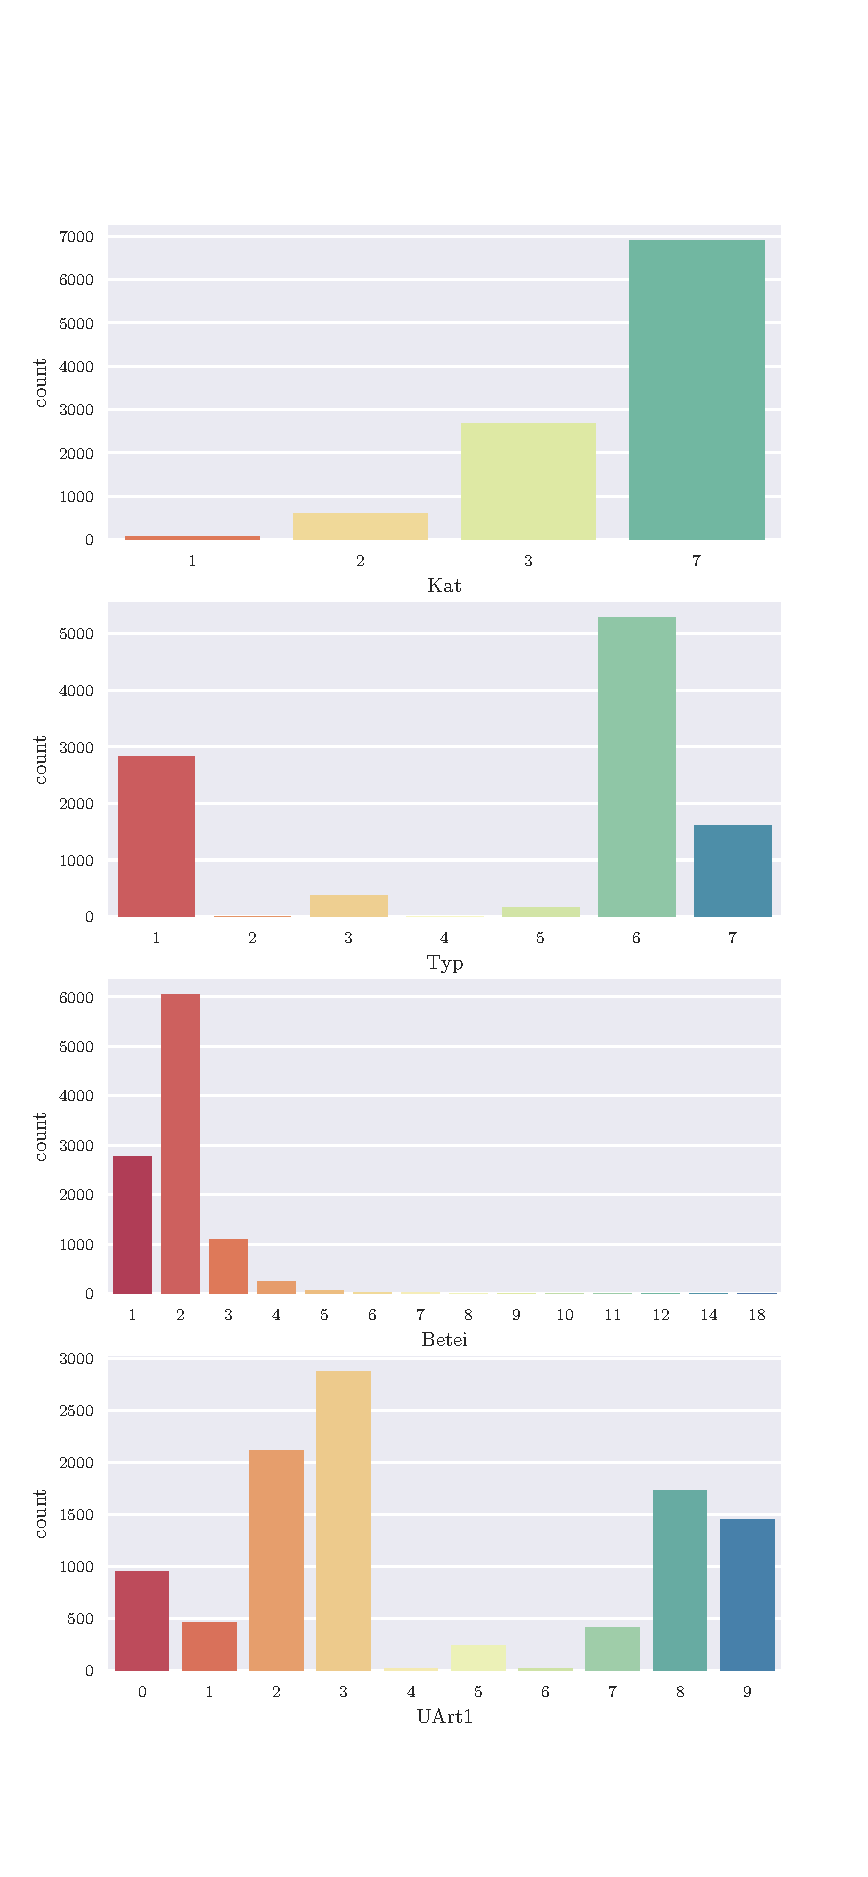
\includegraphics[scale=0.7]{CorrAnalysis/data/BAYSIS/01_dataset/plots/baysis_dataset_count_multiple01}
        \caption{Distribution of the accident category Kat, Typ, Betei and UArt}
        \label{img:baysis_dataset_Kat}
        \label{img:baysis_dataset_Typ}
        \label{img:baysis_dataset_Betei}
        \label{img:baysis_dataset_UArt}
    \end{figure}

    \begin{figure}[ht!]
        \centering
        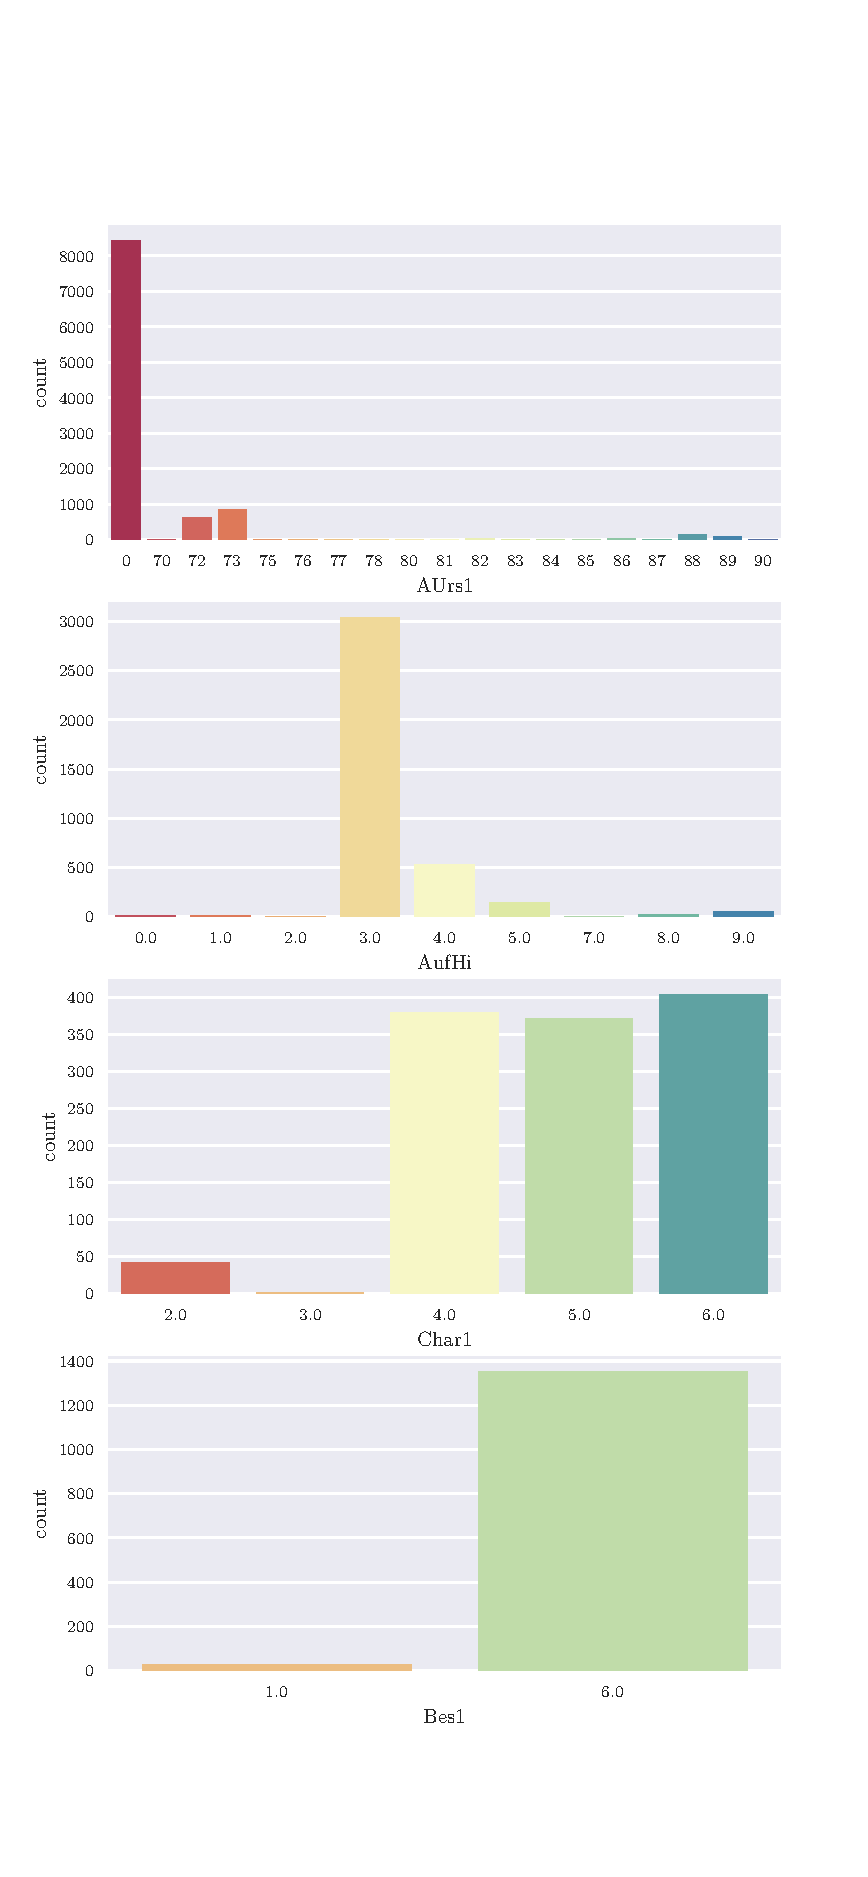
\includegraphics[scale=0.7]{CorrAnalysis/data/BAYSIS/01_dataset/plots/baysis_dataset_count_multiple02}
        \caption{Distribution of the accident category AUrs, AufHi, Char and Bes}
        \label{img:baysis_dataset_AUrs}
        \label{img:baysis_dataset_AufHi}
        \label{img:baysis_dataset_Char}
        \label{img:baysis_dataset_Bes}
    \end{figure}

    \begin{figure}[ht!]
        \centering
        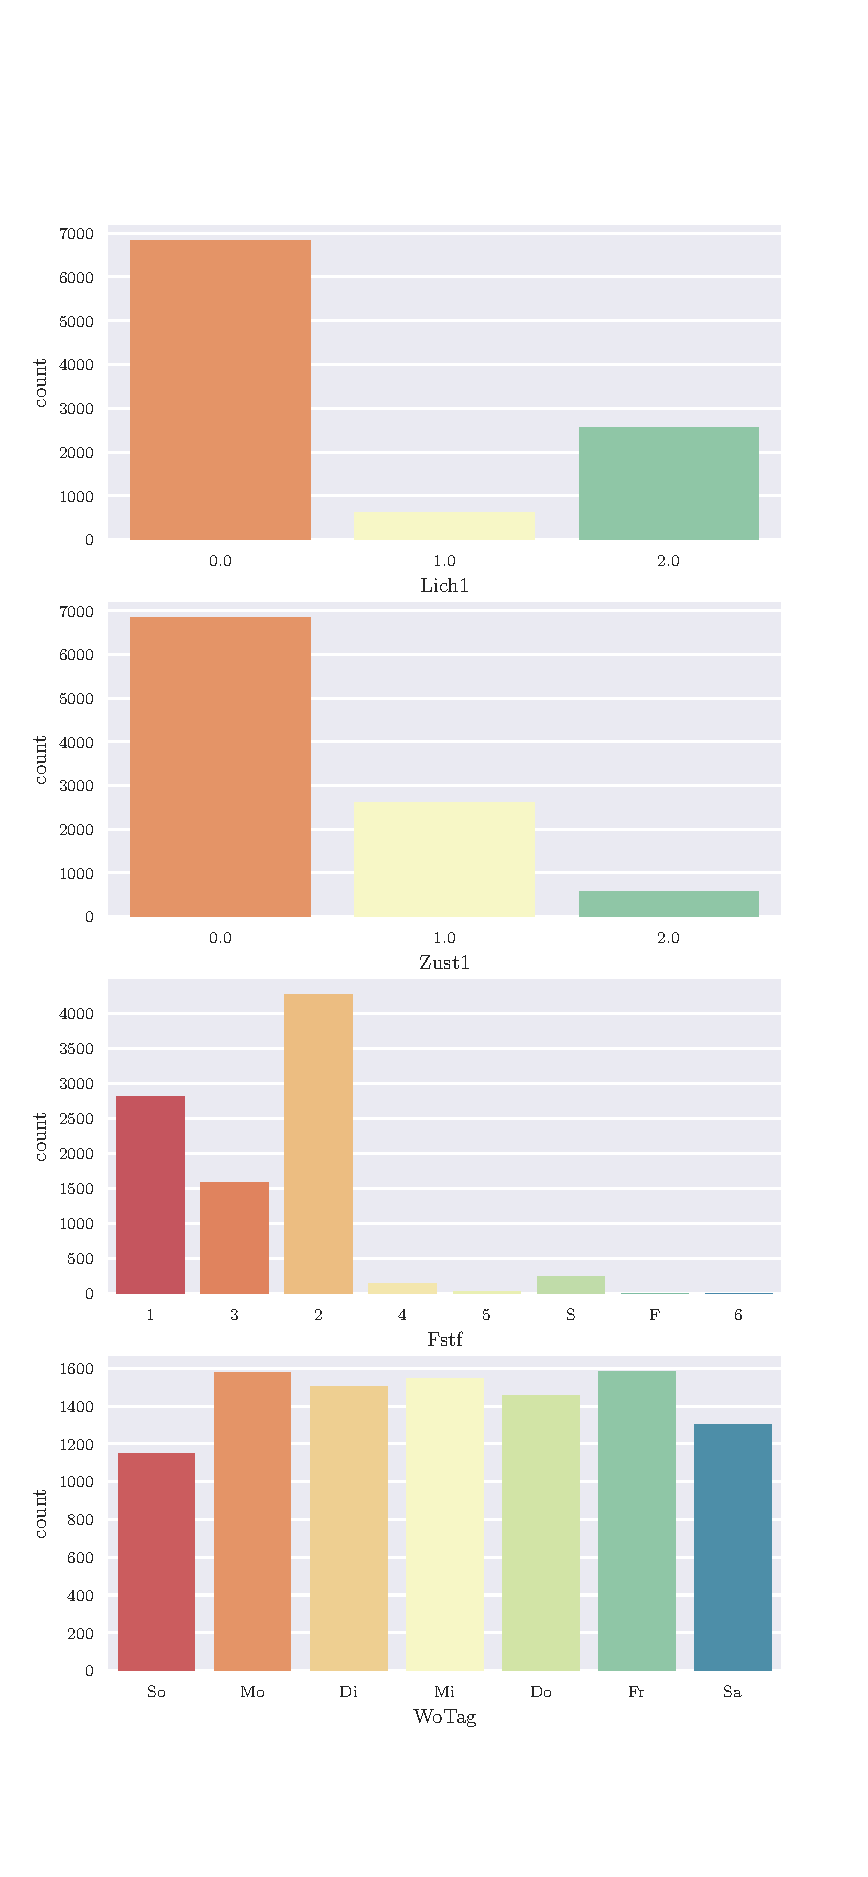
\includegraphics[scale=0.7]{CorrAnalysis/data/BAYSIS/01_dataset/plots/baysis_dataset_count_multiple03}
        \caption{Distribution of the accident category Lich, Zust, Fstf and WoTag}
        \label{img:baysis_dataset_Lich}
        \label{img:baysis_dataset_Zust}
        \label{img:baysis_dataset_Fstf}
        \label{img:baysis_dataset_WoTag}
    \end{figure}

    % ------- BAYSIS Dataset - Tables --------
    % \newgeometry{left=1cm,right=1cm,top=1cm}
    \begin{sidewaystable}
        \tiny
        \setlength{\tabcolsep}{4pt}
        \centering
        \begin{tabular}{lrrrrrrrrrrrrrrrrrrrr}
\toprule
{} &  Strasse &  Kat &  Typ &  Betei &  UArt1 &  UArt2 &  AUrs1 &  AUrs2 &  AufHi &  Alkoh &  Char1 &  Char2 &  Lich1 &  Lich2 &  Zust1 &  Zust2 &  Fstf &  WoTag &  FeiTag &  Month \\
\midrule
Strasse &     1.00 & 0.07 & 0.11 &   0.08 &   0.09 &   0.05 &   0.07 &   0.04 &   0.08 &   0.07 &   0.12 &   0.10 &   0.05 &   0.06 &   0.10 &   0.06 &  0.15 &   0.09 &    0.05 &   0.05 \\
Kat     &     0.07 & 1.00 & 0.16 &   0.18 &   0.31 &   0.10 &   0.08 &   0.05 &   0.12 &   0.02 &   0.05 &   0.03 &   0.02 &   0.04 &   0.05 &   0.02 &  0.08 &   0.04 &    0.03 &   0.05 \\
Typ     &     0.11 & 0.16 & 1.00 &   0.31 &   0.56 &   0.06 &   0.26 &   0.06 &   0.25 &   0.06 &   0.15 &   0.09 &   0.09 &   0.20 &   0.33 &   0.12 &  0.16 &   0.08 &    0.05 &   0.09 \\
Betei   &     0.08 & 0.18 & 0.31 &   1.00 &   0.28 &   0.06 &   0.14 &   0.20 &   0.24 &   0.04 &   0.07 &   0.07 &   0.09 &   0.09 &   0.25 &   0.10 &  0.08 &   0.07 &    0.06 &   0.06 \\
UArt1   &     0.09 & 0.31 & 0.56 &   0.28 &   1.00 &   0.08 &   0.21 &   0.05 &   0.32 &   0.05 &   0.14 &   0.09 &   0.10 &   0.22 &   0.25 &   0.09 &  0.16 &   0.08 &    0.05 &   0.06 \\
UArt2   &     0.05 & 0.10 & 0.06 &   0.06 &   0.08 &   1.00 &   0.06 &   0.03 &   0.15 &   0.04 &   0.03 &   0.05 &   0.03 &   0.05 &   0.08 &   0.04 &  0.04 &   0.04 &    0.01 &   0.04 \\
AUrs1   &     0.07 & 0.08 & 0.26 &   0.14 &   0.21 &   0.06 &   1.00 &   0.20 &   0.16 &   0.05 &   0.08 &   0.09 &   0.12 &   0.13 &   0.66 &   0.77 &  0.05 &   0.09 &    0.04 &   0.15 \\
AUrs2   &     0.04 & 0.05 & 0.06 &   0.20 &   0.05 &   0.03 &   0.20 &   1.00 &   0.06 &   0.04 &   0.03 &   0.06 &   0.04 &   0.03 &   0.12 &   0.33 &  0.03 &   0.03 &    0.03 &   0.05 \\
AufHi   &     0.08 & 0.12 & 0.25 &   0.24 &   0.32 &   0.15 &   0.16 &   0.06 &   1.00 &   0.04 &   0.08 &   0.10 &   0.08 &   0.10 &   0.25 &   0.09 &  0.06 &   0.07 &    0.04 &   0.06 \\
Alkoh   &     0.07 & 0.02 & 0.06 &   0.04 &   0.05 &   0.04 &   0.05 &   0.04 &   0.04 &   1.00 &   0.02 &   0.00 &   0.11 &   0.11 &   0.03 &   0.01 &  0.05 &   0.08 &    0.01 &   0.05 \\
Char1   &     0.12 & 0.05 & 0.15 &   0.07 &   0.14 &   0.03 &   0.08 &   0.03 &   0.08 &   0.02 &   1.00 &   0.58 &   0.04 &   0.05 &   0.10 &   0.03 &  0.06 &   0.03 &    0.02 &   0.04 \\
Char2   &     0.10 & 0.03 & 0.09 &   0.07 &   0.09 &   0.05 &   0.09 &   0.06 &   0.10 &   0.00 &   0.58 &   1.00 &   0.04 &   0.04 &   0.08 &   0.03 &  0.08 &   0.03 &    0.02 &   0.04 \\
Lich1   &     0.05 & 0.02 & 0.09 &   0.09 &   0.10 &   0.03 &   0.12 &   0.04 &   0.08 &   0.11 &   0.04 &   0.04 &   1.00 &   0.71 &   0.16 &   0.06 &  0.05 &   0.04 &    0.03 &   0.21 \\
Lich2   &     0.06 & 0.04 & 0.20 &   0.09 &   0.22 &   0.05 &   0.13 &   0.03 &   0.10 &   0.11 &   0.05 &   0.04 &   0.71 &   1.00 &   0.16 &   0.06 &  0.17 &   0.04 &    0.03 &   0.20 \\
Zust1   &     0.10 & 0.05 & 0.33 &   0.25 &   0.25 &   0.08 &   0.66 &   0.12 &   0.25 &   0.03 &   0.10 &   0.08 &   0.16 &   0.16 &   1.00 &   0.17 &  0.06 &   0.12 &    0.05 &   0.37 \\
Zust2   &     0.06 & 0.02 & 0.12 &   0.10 &   0.09 &   0.04 &   0.77 &   0.33 &   0.09 &   0.01 &   0.03 &   0.03 &   0.06 &   0.06 &   0.17 &   1.00 &  0.05 &   0.06 &    0.02 &   0.17 \\
Fstf    &     0.15 & 0.08 & 0.16 &   0.08 &   0.16 &   0.04 &   0.05 &   0.03 &   0.06 &   0.05 &   0.06 &   0.08 &   0.05 &   0.17 &   0.06 &   0.05 &  1.00 &   0.03 &    0.02 &   0.04 \\
WoTag   &     0.09 & 0.04 & 0.08 &   0.07 &   0.08 &   0.04 &   0.09 &   0.03 &   0.07 &   0.08 &   0.03 &   0.03 &   0.04 &   0.04 &   0.12 &   0.06 &  0.03 &   1.00 &    0.13 &   0.09 \\
FeiTag  &     0.05 & 0.03 & 0.05 &   0.06 &   0.05 &   0.01 &   0.04 &   0.03 &   0.04 &   0.01 &   0.02 &   0.02 &   0.03 &   0.03 &   0.05 &   0.02 &  0.02 &   0.13 &    1.00 &   0.13 \\
Month   &     0.05 & 0.05 & 0.09 &   0.06 &   0.06 &   0.04 &   0.15 &   0.05 &   0.06 &   0.05 &   0.04 &   0.04 &   0.21 &   0.20 &   0.37 &   0.17 &  0.04 &   0.09 &    0.13 &   1.00 \\
\bottomrule
\end{tabular}

        \caption{Correlation matrix for BAYSIS dataset, calculated with Cramer's $V$, $\eta$, $\tau$, $r_{pq}$, $r$}
        \label{table:appendix_correlation_matrix_dataset_cramers}
    \end{sidewaystable}
    \begin{sidewaystable}
        \tiny
        \setlength{\tabcolsep}{4pt}
        \centering
        \begin{tabular}{lrrrrrrrrrrrrrrrrrrrr}
\toprule
{} &  Strasse &  Kat &  Typ &  Betei &  UArt1 &  UArt2 &  AUrs1 &  AUrs2 &  AufHi &  Alkoh &  Char1 &  Char2 &  Lich1 &  Lich2 &  Zust1 &  Zust2 &  Fstf &  WoTag &  FeiTag &  Month \\
\midrule
Strasse &     1.00 & 0.00 & 0.02 &   0.01 &   0.01 &   0.00 &   0.01 &   0.00 &   0.01 &   0.00 &   0.01 &   0.00 &   0.00 &   0.00 &   0.00 &   0.00 &  0.04 &   0.01 &    0.00 &   0.01 \\
Kat     &     0.01 & 1.00 & 0.04 &   0.05 &   0.16 &   0.02 &   0.01 &   0.00 &   0.01 &   0.00 &   0.00 &   0.00 &   0.00 &   0.00 &   0.00 &   0.00 &  0.01 &   0.00 &    0.00 &   0.00 \\
Typ     &     0.03 & 0.03 & 1.00 &   0.26 &   0.39 &   0.01 &   0.15 &   0.01 &   0.17 &   0.00 &   0.02 &   0.00 &   0.01 &   0.02 &   0.09 &   0.01 &  0.05 &   0.02 &    0.00 &   0.02 \\
Betei   &     0.02 & 0.04 & 0.29 &   1.00 &   0.36 &   0.01 &   0.09 &   0.01 &   0.22 &   0.00 &   0.01 &   0.00 &   0.01 &   0.01 &   0.05 &   0.01 &  0.02 &   0.02 &    0.00 &   0.01 \\
UArt1   &     0.02 & 0.07 & 0.25 &   0.20 &   1.00 &   0.02 &   0.07 &   0.00 &   0.25 &   0.00 &   0.01 &   0.00 &   0.01 &   0.01 &   0.03 &   0.00 &  0.05 &   0.01 &    0.00 &   0.01 \\
UArt2   &     0.02 & 0.03 & 0.02 &   0.03 &   0.07 &   1.00 &   0.02 &   0.00 &   0.20 &   0.00 &   0.01 &   0.00 &   0.00 &   0.01 &   0.01 &   0.00 &  0.01 &   0.01 &    0.00 &   0.01 \\
AUrs1   &     0.05 & 0.01 & 0.25 &   0.14 &   0.18 &   0.01 &   1.00 &   0.04 &   0.14 &   0.00 &   0.02 &   0.01 &   0.02 &   0.02 &   0.38 &   0.05 &  0.01 &   0.03 &    0.00 &   0.14 \\
AUrs2   &     0.09 & 0.02 & 0.12 &   0.10 &   0.12 &   0.02 &   0.37 &   1.00 &   0.08 &   0.01 &   0.02 &   0.01 &   0.02 &   0.01 &   0.16 &   0.25 &  0.05 &   0.05 &    0.01 &   0.13 \\
AufHi   &     0.03 & 0.01 & 0.22 &   0.25 &   0.50 &   0.11 &   0.11 &   0.01 &   1.00 &   0.00 &   0.02 &   0.01 &   0.01 &   0.01 &   0.07 &   0.01 &  0.02 &   0.02 &    0.00 &   0.02 \\
Alkoh   &     0.01 & 0.00 & 0.01 &   0.01 &   0.02 &   0.01 &   0.02 &   0.00 &   0.01 &   1.00 &   0.00 &   0.00 &   0.05 &   0.05 &   0.00 &   0.00 &  0.01 &   0.03 &    0.00 &   0.01 \\
Char1   &     0.06 & 0.01 & 0.05 &   0.03 &   0.05 &   0.01 &   0.03 &   0.00 &   0.03 &   0.00 &   1.00 &   0.14 &   0.00 &   0.00 &   0.02 &   0.00 &  0.02 &   0.01 &    0.00 &   0.01 \\
Char2   &     0.05 & 0.00 & 0.03 &   0.02 &   0.03 &   0.01 &   0.03 &   0.01 &   0.04 &   0.00 &   0.60 &   1.00 &   0.01 &   0.01 &   0.03 &   0.00 &  0.02 &   0.00 &    0.00 &   0.01 \\
Lich1   &     0.00 & 0.00 & 0.01 &   0.01 &   0.01 &   0.00 &   0.02 &   0.00 &   0.01 &   0.01 &   0.00 &   0.00 &   1.00 &   0.80 &   0.03 &   0.00 &  0.00 &   0.00 &    0.00 &   0.06 \\
Lich2   &     0.01 & 0.00 & 0.03 &   0.01 &   0.04 &   0.00 &   0.02 &   0.00 &   0.02 &   0.01 &   0.00 &   0.00 &   0.90 &   1.00 &   0.04 &   0.00 &  0.03 &   0.00 &    0.00 &   0.06 \\
Zust1   &     0.01 & 0.00 & 0.14 &   0.08 &   0.08 &   0.01 &   0.36 &   0.02 &   0.08 &   0.00 &   0.01 &   0.00 &   0.03 &   0.03 &   1.00 &   0.04 &  0.00 &   0.02 &    0.00 &   0.14 \\
Zust2   &     0.03 & 0.01 & 0.13 &   0.08 &   0.07 &   0.01 &   0.38 &   0.19 &   0.08 &   0.00 &   0.01 &   0.00 &   0.03 &   0.03 &   0.28 &   1.00 &  0.02 &   0.02 &    0.00 &   0.24 \\
Fstf    &     0.06 & 0.01 & 0.04 &   0.02 &   0.06 &   0.00 &   0.01 &   0.00 &   0.01 &   0.00 &   0.01 &   0.00 &   0.00 &   0.01 &   0.00 &   0.00 &  1.00 &   0.00 &    0.00 &   0.00 \\
WoTag   &     0.01 & 0.00 & 0.01 &   0.01 &   0.01 &   0.00 &   0.01 &   0.00 &   0.01 &   0.00 &   0.00 &   0.00 &   0.00 &   0.00 &   0.01 &   0.00 &  0.00 &   1.00 &    0.00 &   0.01 \\
FeiTag  &     0.01 & 0.00 & 0.01 &   0.01 &   0.01 &   0.00 &   0.01 &   0.00 &   0.01 &   0.00 &   0.00 &   0.00 &   0.00 &   0.00 &   0.01 &   0.00 &  0.00 &   0.07 &    1.00 &   0.10 \\
Month   &     0.01 & 0.00 & 0.01 &   0.01 &   0.01 &   0.00 &   0.04 &   0.00 &   0.01 &   0.00 &   0.00 &   0.00 &   0.02 &   0.02 &   0.04 &   0.01 &  0.00 &   0.01 &    0.00 &   1.00 \\
\bottomrule
\end{tabular}

        \caption{Correlation matrix for BAYSIS dataset, calculated with Theil's $U$, $\eta$, $\tau$, $r_{pq}$, $r$}
        \label{table:appendix_correlation_matrix_dataset_theils}
    \end{sidewaystable}
    \begin{sidewaystable}
        \tiny
        \setlength{\tabcolsep}{4pt}
        \centering
        \begin{tabular}{lrrrrrrrrrrrrrrrrrrrr}
\toprule
{} &  Strasse &   Kat &   Typ &  Betei &  UArt1 &  UArt2 &  AUrs1 &  AUrs2 &  AufHi &  Alkoh &  Char1 &  Char2 &  Lich1 &  Lich2 &  Zust1 &  Zust2 &  Fstf &  WoTag &  FeiTag &  Month \\
\midrule
Strasse &      nan & 0.000 & 0.000 &  0.000 &  0.000 &  0.000 &  0.000 &  0.871 &  0.000 &  0.000 &  0.000 &  0.000 &  0.165 &  0.000 &  0.000 &  0.006 & 0.000 &  0.000 &   0.073 &  0.002 \\
Kat     &    0.000 &   nan & 0.000 &  0.000 &  0.000 &  0.000 &  0.000 &  0.000 &  0.000 &  0.225 &  0.000 &  0.058 &  0.260 &  0.000 &  0.000 &  0.068 & 0.000 &  0.000 &   0.069 &  0.000 \\
Typ     &    0.000 & 0.000 &   nan &  0.000 &  0.000 &  0.000 &  0.000 &  0.000 &  0.000 &  0.000 &  0.000 &  0.000 &  0.000 &  0.000 &  0.000 &  0.000 & 0.000 &  0.000 &   0.000 &  0.000 \\
Betei   &    0.000 & 0.000 & 0.000 &    nan &  0.000 &  0.000 &  0.000 &  0.000 &  0.000 &  0.463 &  0.000 &  0.000 &  0.000 &  0.000 &  0.000 &  0.000 & 0.000 &  0.000 &   0.000 &  0.000 \\
UArt1   &    0.000 & 0.000 & 0.000 &  0.000 &    nan &  0.000 &  0.000 &  0.000 &  0.000 &  0.000 &  0.000 &  0.000 &  0.000 &  0.000 &  0.000 &  0.000 & 0.000 &  0.000 &   0.001 &  0.000 \\
UArt2   &    0.000 & 0.000 & 0.000 &  0.000 &  0.000 &    nan &  0.000 &  0.045 &  0.000 &  0.017 &  0.043 &  0.001 &  0.122 &  0.001 &  0.000 &  0.002 & 0.000 &  0.016 &   0.998 &  0.054 \\
AUrs1   &    0.000 & 0.000 & 0.000 &  0.000 &  0.000 &  0.000 &    nan &  0.000 &  0.000 &  0.157 &  0.000 &  0.000 &  0.000 &  0.000 &  0.000 &  0.000 & 0.002 &  0.000 &   0.386 &  0.000 \\
AUrs2   &    0.871 & 0.000 & 0.000 &  0.000 &  0.000 &  0.045 &  0.000 &    nan &  0.000 &  0.070 &  0.130 &  0.000 &  0.028 &  0.647 &  0.000 &  0.000 & 0.247 &  0.100 &   0.199 &  0.000 \\
AufHi   &    0.000 & 0.000 & 0.000 &  0.000 &  0.000 &  0.000 &  0.000 &  0.000 &    nan &  0.026 &  0.000 &  0.000 &  0.000 &  0.000 &  0.000 &  0.000 & 0.000 &  0.000 &   0.066 &  0.000 \\
Alkoh   &    0.000 & 0.225 & 0.000 &  0.463 &  0.000 &  0.017 &  0.157 &  0.070 &  0.026 &    nan &  0.689 &  0.754 &  0.000 &  0.000 &  0.035 &  0.745 & 0.004 &  0.000 &   0.279 &  0.017 \\
Char1   &    0.000 & 0.000 & 0.000 &  0.000 &  0.000 &  0.043 &  0.000 &  0.130 &  0.000 &  0.689 &    nan &  0.000 &  0.000 &  0.000 &  0.000 &  0.017 & 0.000 &  0.007 &   0.415 &  0.084 \\
Char2   &    0.000 & 0.058 & 0.000 &  0.000 &  0.000 &  0.001 &  0.000 &  0.000 &  0.000 &  0.754 &  0.000 &    nan &  0.001 &  0.000 &  0.000 &  0.012 & 0.000 &  0.250 &   0.020 &  0.075 \\
Lich1   &    0.165 & 0.260 & 0.000 &  0.000 &  0.000 &  0.122 &  0.000 &  0.028 &  0.000 &  0.000 &  0.000 &  0.001 &    nan &  0.000 &  0.000 &  0.000 & 0.000 &  0.002 &   0.015 &  0.000 \\
Lich2   &    0.000 & 0.000 & 0.000 &  0.000 &  0.000 &  0.001 &  0.000 &  0.647 &  0.000 &  0.000 &  0.000 &  0.000 &  0.000 &    nan &  0.000 &  0.000 & 0.000 &  0.001 &   0.033 &  0.000 \\
Zust1   &    0.000 & 0.000 & 0.000 &  0.000 &  0.000 &  0.000 &  0.000 &  0.000 &  0.000 &  0.035 &  0.000 &  0.000 &  0.000 &  0.000 &    nan &  0.000 & 0.000 &  0.000 &   0.000 &  0.000 \\
Zust2   &    0.006 & 0.068 & 0.000 &  0.000 &  0.000 &  0.002 &  0.000 &  0.000 &  0.000 &  0.745 &  0.017 &  0.012 &  0.000 &  0.000 &  0.000 &    nan & 0.000 &  0.000 &   0.125 &  0.000 \\
Fstf    &    0.000 & 0.000 & 0.000 &  0.000 &  0.000 &  0.000 &  0.002 &  0.247 &  0.000 &  0.004 &  0.000 &  0.000 &  0.000 &  0.000 &  0.000 &  0.000 &   nan &  0.033 &   0.660 &  0.081 \\
WoTag   &    0.000 & 0.000 & 0.000 &  0.000 &  0.000 &  0.016 &  0.000 &  0.100 &  0.000 &  0.000 &  0.007 &  0.250 &  0.002 &  0.001 &  0.000 &  0.000 & 0.033 &    nan &   0.000 &  0.000 \\
FeiTag  &    0.073 & 0.069 & 0.000 &  0.000 &  0.001 &  0.998 &  0.386 &  0.199 &  0.066 &  0.279 &  0.415 &  0.020 &  0.015 &  0.033 &  0.000 &  0.125 & 0.660 &  0.000 &     nan &  0.000 \\
Month   &    0.002 & 0.000 & 0.000 &  0.000 &  0.000 &  0.054 &  0.000 &  0.000 &  0.000 &  0.017 &  0.084 &  0.075 &  0.000 &  0.000 &  0.000 &  0.000 & 0.081 &  0.000 &   0.000 &    nan \\
\bottomrule
\end{tabular}

        \caption{Significancy matrix for BAYSIS dataset}
        \label{table:appendix_significancy_matrix_dataset}
    \end{sidewaystable}
    \begin{sidewaystable}
        \tiny
        \setlength{\tabcolsep}{4pt}
        \centering
        \begin{tabular}{lllllllllllllllllllll}
\toprule
{} & Strasse &  Kat &  Typ & Betei & UArt1 & UArt2 & AUrs1 & AUrs2 & AufHi & Alkoh & Char1 & Char2 & Lich1 & Lich2 & Zust1 & Zust2 & Fstf & WoTag & FeiTag & Month \\
\midrule
Strasse &     NaN &  $V$ &  $V$ &   $V$ &   $V$ &   $V$ &   $V$ &   $V$ &   $V$ &   $V$ &   $V$ &   $V$ &   $V$ &   $V$ &   $V$ &   $V$ &  $V$ &   $V$ &    $V$ &   $V$ \\
Kat     &     $V$ &  NaN &  $V$ &   $V$ &   $V$ &   $V$ &   $V$ &   $V$ &   $V$ &   $V$ &   $V$ &   $V$ &   $V$ &   $V$ &   $V$ &   $V$ &  $V$ &   $V$ &    $V$ &   $V$ \\
Typ     &     $V$ &  $V$ &  NaN &   $V$ &   $V$ &   $V$ &   $V$ &   $V$ &   $V$ &   $V$ &   $V$ &   $V$ &   $V$ &   $V$ &   $V$ &   $V$ &  $V$ &   $V$ &    $V$ &   $V$ \\
Betei   &     $V$ &  $V$ &  $V$ &   NaN &   $V$ &   $V$ &   $V$ &   $V$ &   $V$ &   $V$ &   $V$ &   $V$ &   $V$ &   $V$ &   $V$ &   $V$ &  $V$ &   $V$ &    $V$ &   $V$ \\
UArt1   &     $V$ &  $V$ &  $V$ &   $V$ &   NaN &   $V$ &   $V$ &   $V$ &   $V$ &   $V$ &   $V$ &   $V$ &   $V$ &   $V$ &   $V$ &   $V$ &  $V$ &   $V$ &    $V$ &   $V$ \\
UArt2   &     $V$ &  $V$ &  $V$ &   $V$ &   $V$ &   NaN &   $V$ &   $V$ &   $V$ &   $V$ &   $V$ &   $V$ &   $V$ &   $V$ &   $V$ &   $V$ &  $V$ &   $V$ &    $V$ &   $V$ \\
AUrs1   &     $V$ &  $V$ &  $V$ &   $V$ &   $V$ &   $V$ &   NaN &   $V$ &   $V$ &   $V$ &   $V$ &   $V$ &   $V$ &   $V$ &   $V$ &   $V$ &  $V$ &   $V$ &    $V$ &   $V$ \\
AUrs2   &     $V$ &  $V$ &  $V$ &   $V$ &   $V$ &   $V$ &   $V$ &   NaN &   $V$ &   $V$ &   $V$ &   $V$ &   $V$ &   $V$ &   $V$ &   $V$ &  $V$ &   $V$ &    $V$ &   $V$ \\
AufHi   &     $V$ &  $V$ &  $V$ &   $V$ &   $V$ &   $V$ &   $V$ &   $V$ &   NaN &   $V$ &   $V$ &   $V$ &   $V$ &   $V$ &   $V$ &   $V$ &  $V$ &   $V$ &    $V$ &   $V$ \\
Alkoh   &     $V$ &  $V$ &  $V$ &   $V$ &   $V$ &   $V$ &   $V$ &   $V$ &   $V$ &   NaN &   $V$ &   $V$ &   $V$ &   $V$ &   $V$ &   $V$ &  $V$ &   $V$ &    $V$ &   $V$ \\
Char1   &     $V$ &  $V$ &  $V$ &   $V$ &   $V$ &   $V$ &   $V$ &   $V$ &   $V$ &   $V$ &   NaN &   $V$ &   $V$ &   $V$ &   $V$ &   $V$ &  $V$ &   $V$ &    $V$ &   $V$ \\
Char2   &     $V$ &  $V$ &  $V$ &   $V$ &   $V$ &   $V$ &   $V$ &   $V$ &   $V$ &   $V$ &   $V$ &   NaN &   $V$ &   $V$ &   $V$ &   $V$ &  $V$ &   $V$ &    $V$ &   $V$ \\
Lich1   &     $V$ &  $V$ &  $V$ &   $V$ &   $V$ &   $V$ &   $V$ &   $V$ &   $V$ &   $V$ &   $V$ &   $V$ &   NaN &   $V$ &   $V$ &   $V$ &  $V$ &   $V$ &    $V$ &   $V$ \\
Lich2   &     $V$ &  $V$ &  $V$ &   $V$ &   $V$ &   $V$ &   $V$ &   $V$ &   $V$ &   $V$ &   $V$ &   $V$ &   $V$ &   NaN &   $V$ &   $V$ &  $V$ &   $V$ &    $V$ &   $V$ \\
Zust1   &     $V$ &  $V$ &  $V$ &   $V$ &   $V$ &   $V$ &   $V$ &   $V$ &   $V$ &   $V$ &   $V$ &   $V$ &   $V$ &   $V$ &   NaN &   $V$ &  $V$ &   $V$ &    $V$ &   $V$ \\
Zust2   &     $V$ &  $V$ &  $V$ &   $V$ &   $V$ &   $V$ &   $V$ &   $V$ &   $V$ &   $V$ &   $V$ &   $V$ &   $V$ &   $V$ &   $V$ &   NaN &  $V$ &   $V$ &    $V$ &   $V$ \\
Fstf    &     $V$ &  $V$ &  $V$ &   $V$ &   $V$ &   $V$ &   $V$ &   $V$ &   $V$ &   $V$ &   $V$ &   $V$ &   $V$ &   $V$ &   $V$ &   $V$ &  NaN &   $V$ &    $V$ &   $V$ \\
WoTag   &     $V$ &  $V$ &  $V$ &   $V$ &   $V$ &   $V$ &   $V$ &   $V$ &   $V$ &   $V$ &   $V$ &   $V$ &   $V$ &   $V$ &   $V$ &   $V$ &  $V$ &   NaN &    $V$ &   $V$ \\
FeiTag  &     $V$ &  $V$ &  $V$ &   $V$ &   $V$ &   $V$ &   $V$ &   $V$ &   $V$ &   $V$ &   $V$ &   $V$ &   $V$ &   $V$ &   $V$ &   $V$ &  $V$ &   $V$ &    NaN &   $V$ \\
Month   &     $V$ &  $V$ &  $V$ &   $V$ &   $V$ &   $V$ &   $V$ &   $V$ &   $V$ &   $V$ &   $V$ &   $V$ &   $V$ &   $V$ &   $V$ &   $V$ &  $V$ &   $V$ &    $V$ &   NaN \\
\bottomrule
\end{tabular}

        \caption{Coefficient matrix for BAYSIS dataset}
        \label{table:appendix_coefficient_matrix_dataset}
    \end{sidewaystable}
    % \restoregeometry
    
    % -------------------------------
    % ------- BAYSIS Matched --------
    % -------------------------------
    % \tocless\section{BAYSIS Matched Data}
    % \label{appendix_baysis_dataset}
    
    % ------- BAYSIS Matched - Figures --------
    \begin{figure}[ht!]
        \centering
        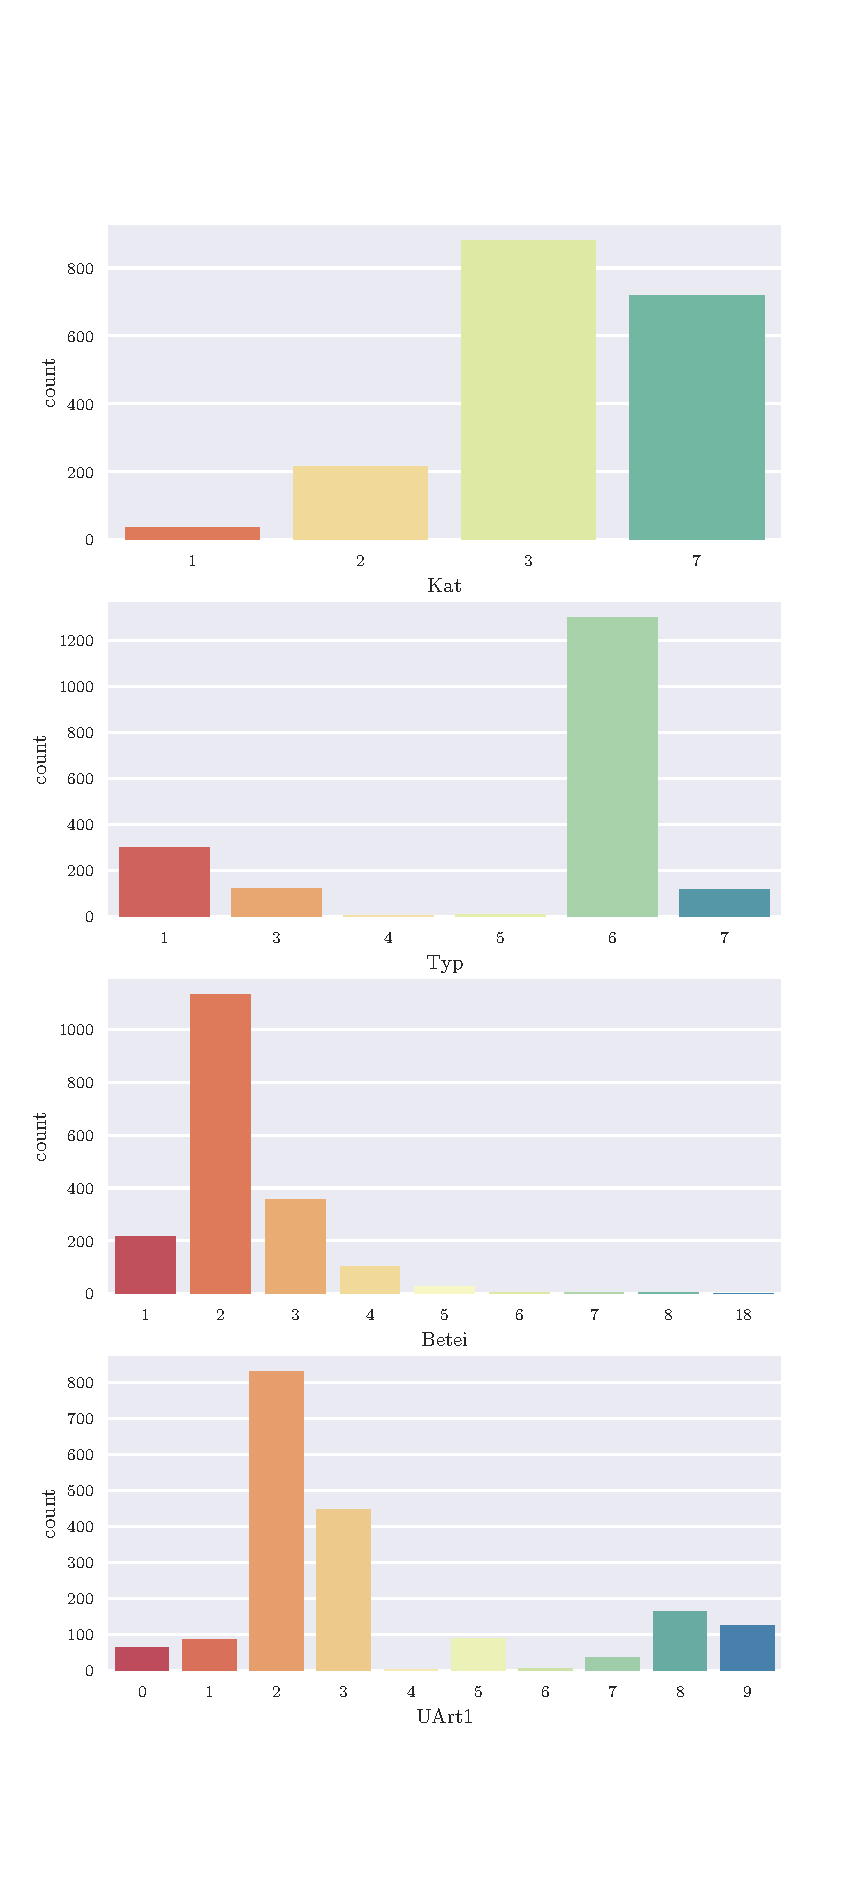
\includegraphics[scale=0.7]{CorrAnalysis/data/BAYSIS/02_matched/plots/baysis_matched_count_multiple01}
        \caption{Distribution of the accident category Kat, Typ, Betei and UArt}
        \label{img:baysis_matched_Kat}
        \label{img:baysis_matched_Typ}
        \label{img:baysis_matched_Betei}
        \label{img:baysis_matched_UArt}
    \end{figure}

    \begin{figure}[ht!]
        \centering
        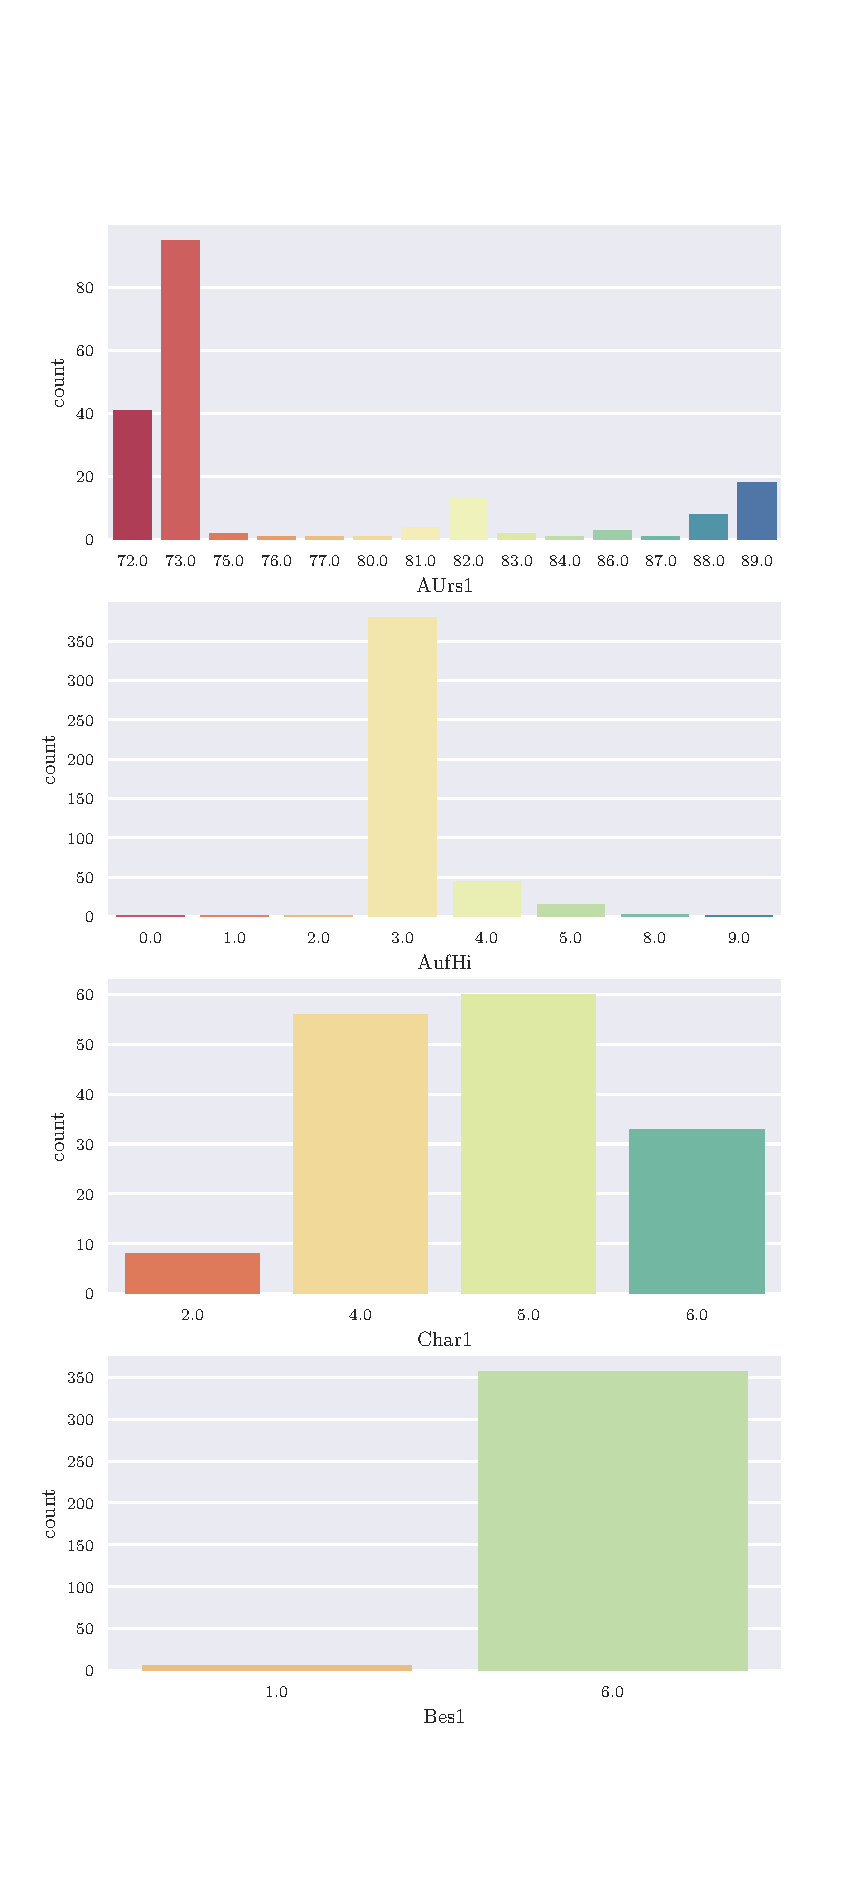
\includegraphics[scale=0.7]{CorrAnalysis/data/BAYSIS/02_matched/plots/baysis_matched_count_multiple02}
        \caption{Distribution of the accident category AUrs, AufHi, Char and Bes}
        \label{img:baysis_matched_AUrs}
        \label{img:baysis_matched_AufHi}
        \label{img:baysis_matched_Char}
        \label{img:baysis_matched_Bes}
    \end{figure}

    \begin{figure}[ht!]
        \centering
        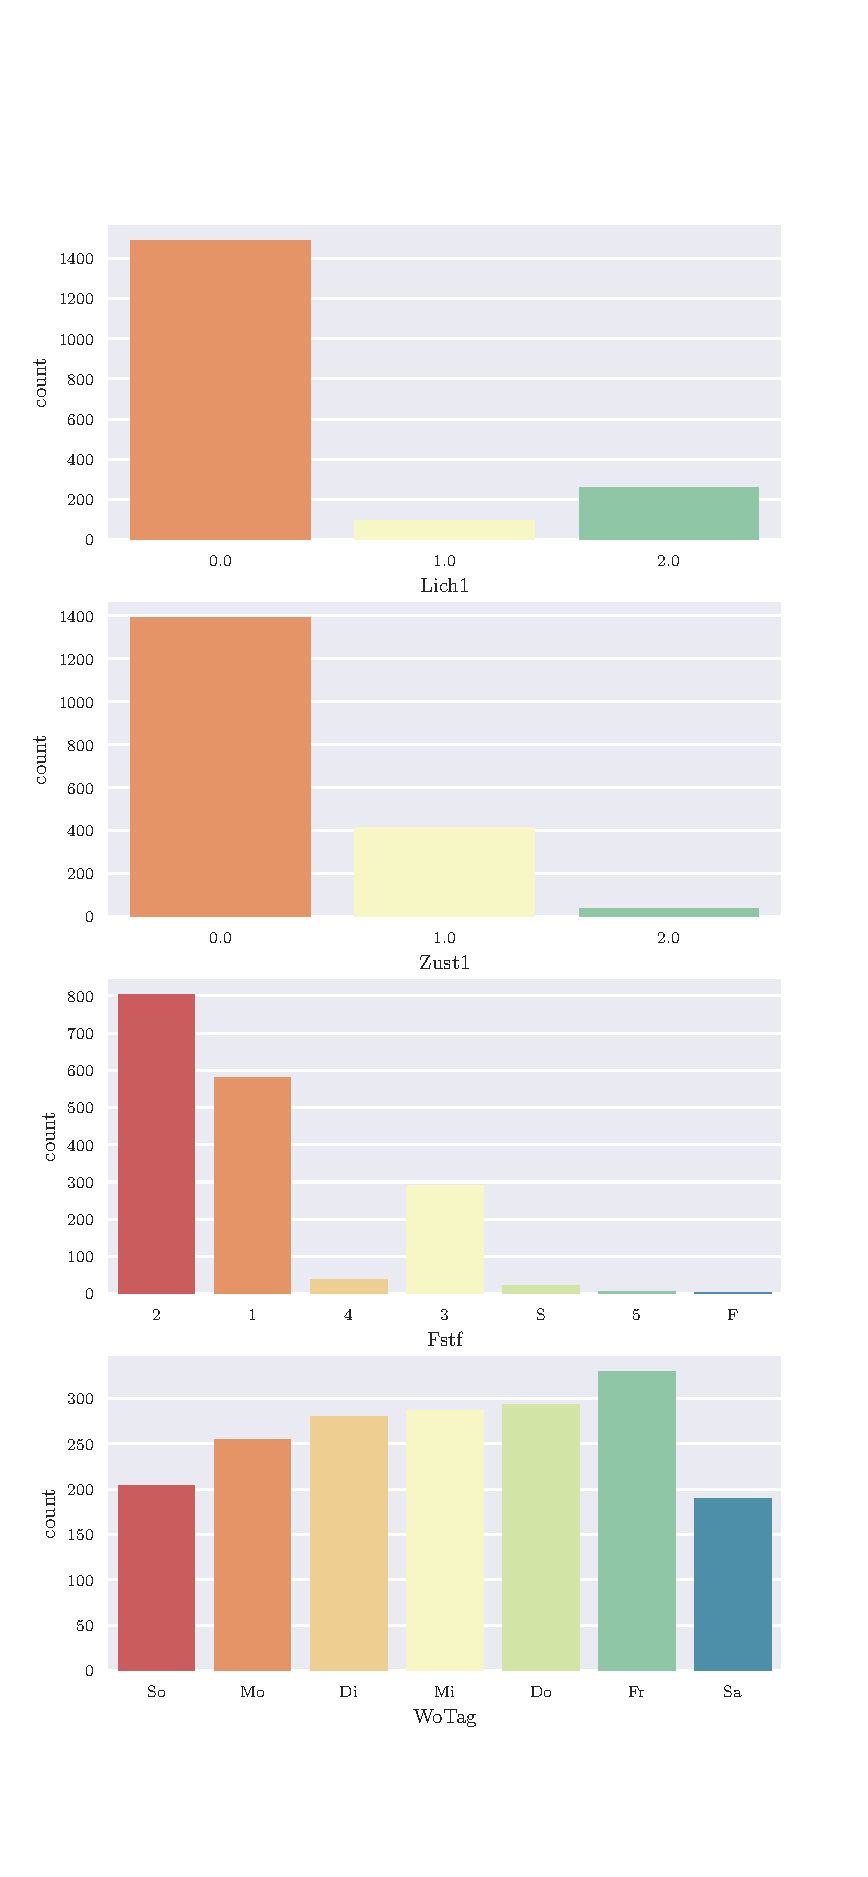
\includegraphics[scale=0.7]{CorrAnalysis/data/BAYSIS/02_matched/plots/baysis_matched_count_multiple03}
        \caption{Distribution of the accident category Lich, Zust, Fstf and WoTag}
        \label{img:baysis_matched_Lich}
        \label{img:baysis_matched_Zust}
        \label{img:baysis_matched_Fstf}
        \label{img:baysis_matched_WoTag}
    \end{figure}

    \begin{table}[ht!]
        \tiny
        \setlength{\tabcolsep}{4pt}
        \centering
        \begin{tabular}{rrrrrrrrrrrrrrrrr}
            \toprule
                    & A3 & A6 & A9 & A70 & A96 & A7 & A73 & A99 & A92 & A93 & A94 & A72 & A995 & A95 & A71 & A45 \\ 
            \midrule
            A6 		& 0.00 &  &  &  &  &  &  &  &  &  &  &  &  &  &  &  \\ 
            A9 		& \red{0.01} & 1.00 &  &  &  &  &  &  &  &  &  &  &  &  &  &  \\ 
            A70 	& \red{0.03} & 1.00 & 1.00 &  &  &  &  &  &  &  &  &  &  &  &  &  \\ 
            A96 	& \red{0.00} & 1.00 & 0.27 & 1.00 &  &  &  &  &  &  &  &  &  &  &  &  \\ 
            A7 		& \red{0.00} & 1.00 & 1.00 & 1.00 & 1.00 &  &  &  &  &  &  &  &  &  &  &  \\ 
            A73 	& \red{0.00} & 1.00 & 0.31 & 1.00 & 1.00 & 1.00 &  &  &  &  &  &  &  &  &  &  \\ 
            A99 	& 1.00 & 1.00 & 1.00 & 1.00 & 0.50 & 1.00 & 0.59 &  &  &  &  &  &  &  &  &  \\ 
            A92 	& \red{0.00} & 1.00 & 0.16 & 1.00 & 1.00 & 1.00 & 1.00 & 0.22 &  &  &  &  &  &  &  &  \\ 
            A93 	& 1.00 & 1.00 & 1.00 & 1.00 & 1.00 & 1.00 & 1.00 & 1.00 & 1.00 &  &  &  &  &  &  &  \\ 
            A94 	& \red{0.01} & 1.00 & 1.00 & 1.00 & 1.00 & 1.00 & 1.00 & 1.00 & 1.00 & 1.00 &  &  &  &  &  &  \\ 
            A72 	& 1.00 & 1.00 & 1.00 & 1.00 & 1.00 & 1.00 & 1.00 & 1.00 & 1.00 & 1.00 & 1.00 &  &  &  &  &  \\ 
            A995 	& 1.00 & 1.00 & 1.00 & 1.00 & 1.00 & 1.00 & 1.00 & 1.00 & 1.00 & 1.00 & 1.00 & 1.00 &  &  &  &  \\ 
            A95 	& 1.00 & 1.00 & 1.00 & 1.00 & 1.00 & 1.00 & 1.00 & 1.00 & 1.00 & 1.00 & 1.00 & 1.00 & 1.00 &  &  &  \\ 
            A71 	& 1.00 & 1.00 & 1.00 & 1.00 & 1.00 & 1.00 & 1.00 & 1.00 & 1.00 & 1.00 & 1.00 & 1.00 & 1.00 & 1.00 &  &  \\ 
            A45 	& 1.00 & 1.00 & 1.00 & 1.00 & 1.00 & 1.00 & 1.00 & 1.00 & 1.00 & 1.00 & 1.00 & 1.00 & 1.00 & 1.00 & 1.00 &  \\ 
            A980 	& 1.00 & 1.00 & 1.00 & 1.00 & 1.00 & 1.00 & 1.00 & 1.00 & 1.00 & 1.00 & 1.00 & 1.00 & 1.00 & 1.00 & 1.00 & 1.00 \\ 
            \bottomrule
        \end{tabular}
        \caption{Pairwise Wilcoxon $T$-test for \textit{Street} and \textit{Maximal Temporal Extent} complete}
        \label{tbl:wilcoxon_baysis_matched_Str_TMax_complete}
    \end{table}

    \begin{table}[ht!]
        \tiny
        \setlength{\tabcolsep}{4pt}
        \centering
        \begin{tabular}{rrrrrrrrrrrrrrrrr}
            \toprule
                    & A3 & A6 & A9 & A70 & A96 & A7 & A73 & A99 & A92 & A93 & A94 & A72 & A995 & A95 & A71 & A45 \\ 
            \midrule
            A6 	 & 0.84 &  &  &  &  &  &  &  &  &  &  &  &  &  &  &  \\ 
            A9 	 & 0.36 & 1.00 &  &  &  &  &  &  &  &  &  &  &  &  &  &  \\ 
            A70	 & 1.00 & 1.00 & 1.00 &  &  &  &  &  &  &  &  &  &  &  &  &  \\ 
            A96  & 0.10 & 1.00 & 1.00 & 1.00 &  &  &  &  &  &  &  &  &  &  &  &  \\ 
            A7 	 & 1.00 & 1.00 & 1.00 & 1.00 & 1.00 &  &  &  &  &  &  &  &  &  &  &  \\ 
            A73  & \red{0.00} & 1.00 & 0.51 & 1.00 & 1.00 & 1.00 &  &  &  &  &  &  &  &  &  &  \\ 
            A99  & \red{0.02} & 1.00 & 1.00 & 1.00 & 1.00 & 1.00 & 1.00 &  &  &  &  &  &  &  &  &  \\ 
            A92  & 0.26 & 1.00 & 1.00 & 1.00 & 1.00 & 1.00 & 1.00 & 1.00 &  &  &  &  &  &  &  &  \\ 
            A93  & 1.00 & 1.00 & 1.00 & 1.00 & 1.00 & 1.00 & 1.00 & 1.00 & 1.00 &  &  &  &  &  &  &  \\ 
            A94  & 0.28 & 1.00 & 1.00 & 1.00 & 1.00 & 1.00 & 1.00 & 1.00 & 1.00 & 1.00 &  &  &  &  &  &  \\ 
            A72  & 1.00 & 1.00 & 1.00 & 1.00 & 1.00 & 1.00 & 1.00 & 1.00 & 1.00 & 1.00 & 1.00 &  &  &  &  &  \\ 
            A995 & 1.00 & 1.00 & 1.00 & 1.00 & 1.00 & 1.00 & 1.00 & 1.00 & 1.00 & 1.00 & 1.00 & 1.00 &  &  &  &  \\ 
            A95  & 1.00 & 1.00 & 1.00 & 1.00 & 1.00 & 1.00 & 1.00 & 1.00 & 1.00 & 1.00 & 1.00 & 1.00 & 1.00 &  &  &  \\ 
            A71	 & 1.00 & 1.00 & 1.00 & 1.00 & 1.00 & 1.00 & 1.00 & 1.00 & 1.00 & 1.00 & 1.00 & 1.00 & 1.00 & 1.00 &  &  \\ 
            A45  & 1.00 & 1.00 & 1.00 & 1.00 & 1.00 & 1.00 & 1.00 & 1.00 & 1.00 & 1.00 & 1.00 & 1.00 & 1.00 & 1.00 & 1.00 &  \\ 
            A980 & 1.00 & 1.00 & 1.00 & 1.00 & 1.00 & 1.00 & 1.00 & 1.00 & 1.00 & 1.00 & 1.00 & 1.00 & 1.00 & 1.00 & 1.00 & 1.00 \\
            \bottomrule
        \end{tabular}
        \caption{Pairwise Wilcoxon $T$-test for \textit{Street} and \textit{Average Temporal Extent} complete}
        \label{tbl:wilcoxon_baysis_matched_Str_TAvg_complete}
    \end{table}

    \begin{table}[ht!]
        \tiny
        \setlength{\tabcolsep}{4pt}
        \centering
        \begin{tabular}{rrrrrrrrrrrrrrrrr}
            \toprule
                    & A3   & A6   & A9   & A70  & A96  & A7   & A73   & A99 & A92 & A93 & A94 & A72 & A995 & A95 & A71 & A45 \\ 
            \midrule
            A6 		& 0.40 &  &  &  &  &  &  &  &  &  &  &  &  &  &  &  \\ 
            A9 		& \red{0.00} & 1.00 &  &  &  &  &  &  &  &  &  &  &  &  &  &  \\ 
            A70 	& \red{0.00} & 0.83 & 0.54 &  &  &  &  &  &  &  &  &  &  &  &  &  \\ 
            A96 	& \red{0.00} & 1.00 & 0.14 & 1.00 &  &  &  &  &  &  &  &  &  &  &  &  \\ 
            A7 		& \red{0.00} & 1.00 & 1.00 & 1.00 & 1.00 &  &  &  &  &  &  &  &  &  &  &  \\ 
            A73 	& \red{0.00} & \red{0.00} & \red{0.00} & 1.00 & 1.00 & 0.59 &  &  &  &  &  &  &  &  &  &  \\ 
            A99 	& 1.00 & 1.00 & 1.00 & 0.80 & 0.31 & 1.00 & \red{0.00} &  &  &  &  &  &  &  &  &  \\ 
            A92 	& \red{0.00} & \red{0.00} & \red{0.00} & 1.00 & 1.00 & 1.00 & 1.00 & \red{0.00} &  &  &  &  &  &  &  &  \\ 
            A93 	& \red{0.03} & 1.00 & 1.00 & 1.00 & 1.00 & 1.00 & 1.00 & 1.00 & 1.00 &  &  &  &  &  &  &  \\ 
            A94 	& \red{0.00} & 0.11 & \red{0.03} & 1.00 & 1.00 & 1.00 & 1.00 & 0.09 & 1.00 & 1.00 &  &  &  &  &  &  \\ 
            A72 	& 1.00 & 1.00 & 1.00 & 1.00 & 1.00 & 1.00 & 1.00 & 1.00 & 1.00 & 1.00 & 1.00 &  &  &  &  &  \\ 
            A995 	& 1.00 & 1.00 & 1.00 & 1.00 & 1.00 & 1.00 & 1.00 & 1.00 & 1.00 & 1.00 & 1.00 & 1.00 &  &  &  &  \\ 
            A95 	& 1.00 & 1.00 & 1.00 & 1.00 & 1.00 & 1.00 & 1.00 & 1.00 & 1.00 & 1.00 & 1.00 & 1.00 & 1.00 &  &  &  \\ 
            A71 	& 1.00 & 1.00 & 1.00 & 1.00 & 1.00 & 1.00 & 1.00 & 1.00 & 1.00 & 1.00 & 1.00 & 1.00 & 1.00 & 1.00 &  &  \\ 
            A45 	& 1.00 & 1.00 & 1.00 & 1.00 & 1.00 & 1.00 & 1.00 & 1.00 & 1.00 & 1.00 & 1.00 & 1.00 & 1.00 & 1.00 & 1.00 &  \\ 
            A980 	& 1.00 & 1.00 & 1.00 & 1.00 & 1.00 & 1.00 & 1.00 & 1.00 & 1.00 & 1.00 & 1.00 & 1.00 & 1.00 & 1.00 & 1.00 & 1.00 \\ 
            \bottomrule
        \end{tabular}
        \caption{Pairwise Wilcoxon $T$-test for \textit{Street} and \textit{Maximal Spatial Extent} complete}
        \label{tbl:wilcoxon_baysis_matched_Str_SMax_complete}
    \end{table}

    \begin{table}[ht!]
        \tiny
        \setlength{\tabcolsep}{4pt}
        \centering
        \begin{tabular}{rrrrrrrrrrrrrrrrr}
            \toprule
                & A3 & A6 & A9 & A70 & A96 & A7 & A73 & A99 & A92 & A93 & A94 & A72 & A995 & A95 & A71 & A45 \\ 
            \midrule
            A6   & 1.00 &  &  &  &  &  &  &  &  &  &  &  &  &  &  &  \\ 
            A9   & 1.00 & 1.00 &  &  &  &  &  &  &  &  &  &  &  &  &  &  \\ 
            A70  & \red{0.05} & 0.83 & 0.71 &  &  &  &  &  &  &  &  &  &  &  &  &  \\ 
            A96  & \red{0.05} & 1.00 & 1.00 & 1.00 &  &  &  &  &  &  &  &  &  &  &  &  \\ 
            A7   & 1.00 & 1.00 & 1.00 & 1.00 & 1.00 &  &  &  &  &  &  &  &  &  &  &  \\ 
            A73  & \red{0.00} & \red{0.00} & \red{0.00} & 1.00 & \red{0.00} & \red{0.00} &  &  &  &  &  &  &  &  &  &  \\ 
            A99  & \red{0.00} & 1.00 & 0.06 & 1.00 & 1.00 & 1.00 & 0.51 &  &  &  &  &  &  &  &  &  \\ 
            A92  & \red{0.00} & 0.61 & \red{0.03} & 1.00 & 1.00 & 1.00 & 1.00 & 1.00 &  &  &  &  &  &  &  &  \\ 
            A93  & \red{0.03} & 0.46 & 0.16 & 1.00 & 1.00 & 1.00 & 1.00 & 1.00 & 1.00 &  &  &  &  &  &  &  \\ 
            A94  & \red{0.00} & 0.07 & 0.01 & 1.00 & 0.36 & 0.31 & 1.00 & 1.00 & 1.00 & 1.00 &  &  &  &  &  &  \\ 
            A72  & 1.00 & 1.00 & 1.00 & 1.00 & 1.00 & 1.00 & 1.00 & 1.00 & 1.00 & 1.00 & 1.00 &  &  &  &  &  \\ 
            A995 & 1.00 & 1.00 & 1.00 & 1.00 & 1.00 & 1.00 & 1.00 & 1.00 & 1.00 & 1.00 & 1.00 & 1.00 &  &  &  &  \\ 
            A95  & 1.00 & 1.00 & 1.00 & 1.00 & 1.00 & 1.00 & 1.00 & 1.00 & 1.00 & 1.00 & 1.00 & 1.00 & 1.00 &  &  &  \\ 
            A71  & 1.00 & 1.00 & 1.00 & 1.00 & 1.00 & 1.00 & 1.00 & 1.00 & 1.00 & 1.00 & 1.00 & 1.00 & 1.00 & 1.00 &  &  \\ 
            A45  & 1.00 & 1.00 & 1.00 & 1.00 & 1.00 & 1.00 & 1.00 & 1.00 & 1.00 & 1.00 & 1.00 & 1.00 & 1.00 & 1.00 & 1.00 &  \\ 
            A980 & 1.00 & 1.00 & 1.00 & 1.00 & 1.00 & 1.00 & 1.00 & 1.00 & 1.00 & 1.00 & 1.00 & 1.00 & 1.00 & 1.00 & 1.00 & 1.00 \\ 
            \bottomrule
        \end{tabular}
        \caption{Pairwise Wilcoxon $T$-test for \textit{Street} and \textit{Average Spatial Extent} complete}
        \label{tbl:wilcoxon_baysis_matched_Str_SAvg_complete}
    \end{table}

    \begin{table}[ht!]
        \tiny
        \setlength{\tabcolsep}{4pt}
        \centering
        \begin{tabular}{rrrrrrrrrrrrrrrrr}
            \toprule
                    & A3   & A6   & A9   & A70  & A96  & A7   & A73 & A99 & A92 & A93 & A94 & A72 & A995 & A95 & A71 & A45 \\ 
            \midrule
            A6 		& \red{0.05} &  &  &  &  &  &  &  &  &  &  &  &  &  &  &  \\ 
            A9 		& \red{0.00} & 1.00 &  &  &  &  &  &  &  &  &  &  &  &  &  &  \\ 
            A70 	& 1.00 & 1.00 & 1.00 &  &  &  &  &  &  &  &  &  &  &  &  &  \\ 
            A96 	& \red{0.00} & 1.00 & \red{0.00} & 1.00 &  &  &  &  &  &  &  &  &  &  &  &  \\ 
            A7 		& \red{0.00} & 1.00 & \red{0.01} & 1.00 & 1.00 &  &  &  &  &  &  &  &  &  &  &  \\ 
            A73 	& \red{0.04} & 1.00 & 1.00 & 1.00 & 1.00 & 1.00 &  &  &  &  &  &  &  &  &  &  \\ 
            A99 	& 0.88 & \red{0.00} & \red{0.00} & 0.09 & \red{0.00} & \red{0.00} & \red{0.00} &  &  &  &  &  &  &  &  &  \\ 
            A92 	& \red{0.00} & 1.00 & 0.12 & 1.00 & 1.00 & 1.00 & 1.00 & \red{0.00} &  &  &  &  &  &  &  &  \\ 
            A93 	& 1.00 & 1.00 & 1.00 & 1.00 & 1.00 & 1.00 & 1.00 & 1.00 & 1.00 &  &  &  &  &  &  &  \\ 
            A94 	& 1.00 & 1.00 & 1.00 & 1.00 & 1.00 & 1.00 & 1.00 & 0.13 & 1.00 & 1.00 &  &  &  &  &  &  \\ 
            A72 	& 1.00 & 1.00 & 1.00 & 1.00 & 1.00 & 1.00 & 1.00 & 1.00 & 1.00 & 1.00 & 1.00 &  &  &  &  &  \\ 
            A995 	& 1.00 & 1.00 & 1.00 & 1.00 & 1.00 & 1.00 & 1.00 & 1.00 & 1.00 & 1.00 & 1.00 & 1.00 &  &  &  &  \\ 
            A95 	& 1.00 & 1.00 & 1.00 & 1.00 & 1.00 & 1.00 & 1.00 & 1.00 & 1.00 & 1.00 & 1.00 & 1.00 & 1.00 &  &  &  \\ 
            A71 	& 1.00 & 1.00 & 1.00 & 1.00 & 1.00 & 1.00 & 1.00 & 1.00 & 1.00 & 1.00 & 1.00 & 1.00 & 1.00 & 1.00 &  &  \\ 
            A45 	& 1.00 & 1.00 & 1.00 & 1.00 & 1.00 & 1.00 & 1.00 & 1.00 & 1.00 & 1.00 & 1.00 & 1.00 & 1.00 & 1.00 & 1.00 &  \\ 
            A980 	& 1.00 & 1.00 & 1.00 & 1.00 & 1.00 & 1.00 & 1.00 & 1.00 & 1.00 & 1.00 & 1.00 & 1.00 & 1.00 & 1.00 & 1.00 & 1.00 \\ 
            \bottomrule
        \end{tabular}
        \caption{Pairwise Wilcoxon $T$-test for \textit{Street} and \textit{Coverage} complete}
        \label{tbl:wilcoxon_baysis_matched_Str_Cov_complete}
    \end{table}

    \begin{table}[ht!]
        \tiny
        \centering
        \begin{tabular}{rrrrrrrrrr}
              \toprule
              & 0 & 1 & 2 & 3 & 4 & 5 & 6 & 7 & 8 \\ 
            \midrule
            % 1 & 1.00 &  &  &  &  &  &  &  &  \\ 
            % 2 & 1.00 & 1.00 &  &  &  &  &  &  &  \\ 
            % 3 & 1.00 & 1.00 & 1.00 &  &  &  &  &  &  \\ 
            % 4 & 0.57 & 0.22 & 0.31 & 0.17 &  &  &  &  &  \\ 
            5 & \red{0.04} & 0.17 & \red{0.00} & \red{0.00} & \red{0.01} &  &  &  &  \\ 
            6 & 0.40 & 0.19 & 0.23 & 0.16 & 1.00 & \red{0.01} &  &  &  \\ 
            7 & \red{0.00} & \red{0.00} & \red{0.00} & \red{0.00} & 1.00 & \red{0.00} & 1.00 &  &  \\ 
            8 & \red{0.02} & \red{0.00} & \red{0.00} & \red{0.00} & 1.00 & \red{0.00} & 1.00 & 0.32 &  \\ 
            9 & \red{0.01} & \red{0.00} & \red{0.00} & \red{0.00} & 1.00 & \red{0.00} & 1.00 & 0.50 & 1.00 \\ 
            \bottomrule
        \end{tabular}
        \caption{Pairwise Wilcoxon $T$-test for \textit{UArt} and \textit{Temporal Distance} complete}
        \label{tbl:wilcoxon_baysis_matched_UArt1_TDist_complete}
    \end{table}

    \begin{table}[ht!]
        \tiny
        \centering
        \begin{tabular}{rrrrrrrrrr}
            \toprule
              & 0 & 1 & 2 & 3 & 4 & 5 & 6 & 7 & 8 \\ 
            \midrule
            % 1 & 1.00 &  &  &  &  &  &  &  &  \\ 
            % 2 & 1.00 & 1.00 &  &  &  &  &  &  &  \\ 
            % 3 & 1.00 & 1.00 & 1.00 &  &  &  &  &  &  \\ 
            % 4 & 1.00 & 1.00 & 1.00 & 1.00 &  &  &  &  &  \\ 
            5 & 0.41 & 0.10 & \red{0.00} & \red{0.01} & 0.65 &  &  &  &  \\ 
            % 6 & 1.00 & 1.00 & 1.00 & 1.00 & 1.00 & 1.00 &  &  &  \\ 
            7 & 0.30 & 0.36 & 0.12 & \red{0.05} & 1.00 & \red{0.00} & 1.00 &  &  \\ 
            8 & \red{0.01} & \red{0.01} & \red{0.00} & \red{0.00} & 1.00 & \red{0.00} & 1.00 & 1.00 &  \\ 
            9 & \red{0.05} & 0.07 & \red{0.00} & \red{0.00} & 1.00 & \red{0.00} & 1.00 & 1.00 & 1.00 \\ 
            \bottomrule
        \end{tabular}
        \caption{Pairwise Wilcoxon $T$-test for \textit{UArt} and \textit{Coverage} complete}
        \label{tbl:wilcoxon_baysis_matched_UArt1_Cov_complete}
    \end{table}

    % ------- BAYSIS Matched - Tables --------
    % \newgeometry{left=1cm,right=1cm,bottom=2cm}
    \begin{sidewaystable}
    	\tiny
    	\setlength{\tabcolsep}{2pt}
    	\centering
    	\begin{tabular}{lrrrrrrrrrrrrrrrrrrrrrrrrrrrrr}
\toprule
{} &  TMax &  TAvg &  SMax &  SAvg &  TDist &  SDist &   Cov &  TLCar &  TLHGV &  Str &  Kat &  Typ &  Betei &  UArt1 &  UArt2 &  AUrs1 &  AUrs2 &  AufHi &  Alkoh &  Char1 &  Char2 &  Lich1 &  Lich2 &  Zust1 &  Zust2 &  Fstf &  WoTag &  FeiTag &  Month \\
\midrule
TMax   &  1.00 &  0.82 &  0.58 &  0.49 &  -0.29 &  -0.09 & -0.25 &   0.03 &  -0.01 & 0.25 & 0.15 & 0.06 &   0.09 &   0.12 &   0.08 &   0.14 &   0.06 &   0.14 &  -0.01 &   0.05 &   0.04 &   0.03 &   0.03 &   0.11 &   0.01 & -0.00 &   0.10 &   -0.00 &   0.14 \\
TAvg   &  0.82 &  1.00 &  0.30 &  0.51 &  -0.16 &  -0.07 &  0.10 &   0.02 &  -0.01 & 0.17 & 0.16 & 0.06 &   0.08 &   0.09 &   0.05 &   0.11 &   0.08 &   0.14 &   0.02 &   0.01 &   0.02 &   0.03 &   0.02 &   0.06 &   0.05 &  0.01 &   0.09 &   -0.01 &   0.10 \\
SMax   &  0.58 &  0.30 &  1.00 &  0.64 &  -0.27 &  -0.09 & -0.50 &   0.01 &  -0.05 & 0.31 & 0.10 & 0.09 &   0.08 &   0.18 &   0.08 &   0.14 &   0.06 &   0.13 &  -0.04 &   0.05 &   0.03 &   0.08 &   0.07 &   0.08 &   0.05 &  0.03 &   0.08 &   -0.00 &   0.15 \\
SAvg   &  0.49 &  0.51 &  0.64 &  1.00 &  -0.09 &  -0.13 &  0.10 &   0.01 &  -0.06 & 0.25 & 0.23 & 0.10 &   0.09 &   0.19 &   0.06 &   0.17 &   0.11 &   0.06 &  -0.02 &   0.04 &   0.00 &   0.02 &   0.02 &   0.01 &   0.12 &  0.04 &   0.11 &    0.01 &   0.11 \\
TDist  & -0.29 & -0.16 & -0.27 & -0.09 &   1.00 &   0.05 &  0.31 &  -0.02 &   0.02 & 0.17 & 0.19 & 0.24 &  -0.04 &   0.29 &   0.11 &   0.20 &   0.11 &   0.21 &   0.04 &   0.11 &   0.11 &   0.13 &   0.14 &   0.13 &   0.02 &  0.03 &   0.10 &    0.01 &   0.10 \\
SDist  & -0.09 & -0.07 & -0.09 & -0.13 &   0.05 &   1.00 & -0.04 &  -0.02 &   0.02 & 0.22 & 0.10 & 0.05 &  -0.03 &   0.07 &   0.06 &   0.15 &   0.02 &   0.02 &  -0.03 &   0.07 &   0.02 &   0.05 &   0.05 &   0.05 &   0.01 &  0.04 &   0.08 &   -0.00 &   0.07 \\
Cov    & -0.25 &  0.10 & -0.50 &  0.10 &   0.31 &  -0.04 &  1.00 &  -0.00 &   0.01 & 0.29 & 0.13 & 0.21 &  -0.02 &   0.24 &   0.12 &   0.22 &   0.10 &   0.21 &   0.07 &   0.11 &   0.08 &   0.15 &   0.15 &   0.17 &   0.03 &  0.02 &   0.16 &    0.01 &   0.14 \\
TLCar  &  0.03 &  0.02 &  0.01 &  0.01 &  -0.02 &  -0.02 & -0.00 &   1.00 &   0.00 & 0.08 & 0.02 & 0.06 &   0.01 &   0.08 &   0.05 &   0.08 &   0.05 &   0.04 &  -0.03 &   0.04 &   0.04 &   0.03 &   0.02 &   0.03 &   0.02 & -0.03 &   0.04 &   -0.01 &   0.04 \\
TLHGV  & -0.01 & -0.01 & -0.05 & -0.06 &   0.02 &   0.02 &  0.01 &   0.00 &   1.00 & 0.11 & 0.02 & 0.06 &  -0.02 &   0.06 &   0.04 &   0.14 &   0.08 &   0.06 &  -0.00 &   0.05 &   0.02 &   0.03 &   0.03 &   0.06 &   0.02 & -0.01 &   0.07 &    0.04 &   0.12 \\
Str    &  0.25 &  0.17 &  0.31 &  0.25 &   0.17 &   0.22 &  0.29 &   0.08 &   0.11 & 1.00 & 0.13 & 0.13 &   0.10 &   0.11 &   0.11 &   0.10 &   0.06 &   0.11 &   0.07 &   0.14 &   0.10 &   0.11 &   0.10 &   0.15 &   0.12 &  0.16 &   0.12 &    0.11 &   0.11 \\
Kat    &  0.15 &  0.16 &  0.10 &  0.23 &   0.19 &   0.10 &  0.13 &   0.02 &   0.02 & 0.13 & 1.00 & 0.20 &   0.21 &   0.35 &   0.13 &   0.11 &   0.05 &   0.15 &   0.05 &   0.08 &   0.07 &   0.06 &   0.06 &   0.06 &   0.07 &  0.09 &   0.09 &    0.07 &   0.10 \\
Typ    &  0.06 &  0.06 &  0.09 &  0.10 &   0.24 &   0.05 &  0.21 &   0.06 &   0.06 & 0.13 & 0.20 & 1.00 &   0.31 &   0.59 &   0.09 &   0.25 &   0.08 &   0.24 &   0.10 &   0.13 &   0.19 &   0.07 &   0.09 &   0.23 &   0.13 &  0.13 &   0.10 &    0.10 &   0.09 \\
Betei  &  0.09 &  0.08 &  0.08 &  0.09 &  -0.04 &  -0.03 & -0.02 &   0.01 &  -0.02 & 0.10 & 0.21 & 0.31 &   1.00 &   0.29 &   0.08 &   0.18 &   0.30 &   0.21 &   0.04 &   0.08 &   0.15 &   0.08 &   0.06 &   0.17 &   0.28 &  0.09 &   0.09 &    0.20 &   0.08 \\
UArt1  &  0.12 &  0.09 &  0.18 &  0.19 &   0.29 &   0.07 &  0.24 &   0.08 &   0.06 & 0.11 & 0.35 & 0.59 &   0.29 &   1.00 &   0.13 &   0.22 &   0.10 &   0.31 &   0.10 &   0.16 &   0.17 &   0.08 &   0.08 &   0.20 &   0.09 &  0.14 &   0.11 &    0.08 &   0.08 \\
UArt2  &  0.08 &  0.05 &  0.08 &  0.06 &   0.11 &   0.06 &  0.12 &   0.05 &   0.04 & 0.11 & 0.13 & 0.09 &   0.08 &   0.13 &   1.00 &   0.15 &   0.05 &   0.26 &   0.02 &   0.08 &   0.11 &   0.07 &   0.07 &   0.07 &   0.05 &  0.06 &   0.07 &    0.04 &   0.08 \\
AUrs1  &  0.14 &  0.11 &  0.14 &  0.17 &   0.20 &   0.15 &  0.22 &   0.08 &   0.14 & 0.10 & 0.11 & 0.25 &   0.18 &   0.22 &   0.15 &   1.00 &   0.45 &   0.16 &   0.03 &   0.10 &   0.15 &   0.13 &   0.10 &   0.59 &   0.49 &  0.07 &   0.10 &    0.35 &   0.14 \\
AUrs2  &  0.06 &  0.08 &  0.06 &  0.11 &   0.11 &   0.02 &  0.10 &   0.05 &   0.08 & 0.06 & 0.05 & 0.08 &   0.30 &   0.10 &   0.05 &   0.45 &   1.00 &   0.04 &   0.01 &   0.04 &   0.11 &   0.06 &   0.03 &   0.20 &   0.45 &  0.03 &   0.07 &    0.32 &   0.08 \\
AufHi  &  0.14 &  0.14 &  0.13 &  0.06 &   0.21 &   0.02 &  0.21 &   0.04 &   0.06 & 0.11 & 0.15 & 0.24 &   0.21 &   0.31 &   0.26 &   0.16 &   0.04 &   1.00 &   0.02 &   0.09 &   0.18 &   0.06 &   0.06 &   0.19 &   0.06 &  0.09 &   0.09 &    0.07 &   0.08 \\
Alkoh  & -0.01 &  0.02 & -0.04 & -0.02 &   0.04 &  -0.03 &  0.07 &  -0.03 &  -0.00 & 0.07 & 0.05 & 0.10 &   0.04 &   0.10 &   0.02 &   0.03 &   0.01 &   0.02 &   1.00 &   0.06 &   0.00 &   0.13 &   0.11 &   0.02 &   0.01 &  0.06 &   0.05 &    0.02 &   0.06 \\
Char1  &  0.05 &  0.01 &  0.05 &  0.04 &   0.11 &   0.07 &  0.11 &   0.04 &   0.05 & 0.14 & 0.08 & 0.13 &   0.08 &   0.16 &   0.08 &   0.10 &   0.04 &   0.09 &   0.06 &   1.00 &   0.59 &   0.07 &   0.06 &   0.09 &   0.03 &  0.06 &   0.06 &    0.03 &   0.08 \\
Char2  &  0.04 &  0.02 &  0.03 &  0.00 &   0.11 &   0.02 &  0.08 &   0.04 &   0.02 & 0.10 & 0.07 & 0.19 &   0.15 &   0.17 &   0.11 &   0.15 &   0.11 &   0.18 &   0.00 &   0.59 &   1.00 &   0.07 &   0.07 &   0.12 &   0.00 &  0.12 &   0.09 &    0.05 &   0.07 \\
Lich1  &  0.03 &  0.03 &  0.08 &  0.02 &   0.13 &   0.05 &  0.15 &   0.03 &   0.03 & 0.11 & 0.06 & 0.07 &   0.08 &   0.08 &   0.07 &   0.13 &   0.06 &   0.06 &   0.13 &   0.07 &   0.07 &   1.00 &   0.71 &   0.15 &   0.03 &  0.06 &   0.07 &    0.03 &   0.25 \\
Lich2  &  0.03 &  0.02 &  0.07 &  0.02 &   0.14 &   0.05 &  0.15 &   0.02 &   0.03 & 0.10 & 0.06 & 0.09 &   0.06 &   0.08 &   0.07 &   0.10 &   0.03 &   0.06 &   0.11 &   0.06 &   0.07 &   0.71 &   1.00 &   0.15 &   0.01 &  0.05 &   0.07 &    0.02 &   0.25 \\
Zust1  &  0.11 &  0.06 &  0.08 &  0.01 &   0.13 &   0.05 &  0.17 &   0.03 &   0.06 & 0.15 & 0.06 & 0.23 &   0.17 &   0.20 &   0.07 &   0.59 &   0.20 &   0.19 &   0.02 &   0.09 &   0.12 &   0.15 &   0.15 &   1.00 &   0.18 &  0.07 &   0.09 &    0.13 &   0.33 \\
Zust2  &  0.01 &  0.05 &  0.05 &  0.12 &   0.02 &   0.01 &  0.03 &   0.02 &   0.02 & 0.12 & 0.07 & 0.13 &   0.28 &   0.09 &   0.05 &   0.49 &   0.45 &   0.06 &   0.01 &   0.03 &   0.00 &   0.03 &   0.01 &   0.18 &   1.00 &  0.02 &   0.07 &    1.00 &   0.22 \\
Fstf   & -0.00 &  0.01 &  0.03 &  0.04 &   0.03 &   0.04 &  0.02 &  -0.03 &  -0.01 & 0.16 & 0.09 & 0.13 &   0.09 &   0.14 &   0.06 &   0.07 &   0.03 &   0.09 &   0.06 &   0.06 &   0.12 &   0.06 &   0.05 &   0.07 &   0.02 &  1.00 &   0.06 &    0.04 &   0.08 \\
WoTag  &  0.10 &  0.09 &  0.08 &  0.11 &   0.10 &   0.08 &  0.16 &   0.04 &   0.07 & 0.12 & 0.09 & 0.10 &   0.09 &   0.11 &   0.07 &   0.10 &   0.07 &   0.09 &   0.05 &   0.06 &   0.09 &   0.07 &   0.07 &   0.09 &   0.07 &  0.06 &   1.00 &    0.12 &   0.12 \\
FeiTag & -0.00 & -0.01 & -0.00 &  0.01 &   0.01 &  -0.00 &  0.01 &  -0.01 &   0.04 & 0.11 & 0.07 & 0.10 &   0.20 &   0.08 &   0.04 &   0.35 &   0.32 &   0.07 &   0.02 &   0.03 &   0.05 &   0.03 &   0.02 &   0.13 &   1.00 &  0.04 &   0.12 &    1.00 &   0.20 \\
Month  &  0.14 &  0.10 &  0.15 &  0.11 &   0.10 &   0.07 &  0.14 &   0.04 &   0.12 & 0.11 & 0.10 & 0.09 &   0.08 &   0.08 &   0.08 &   0.14 &   0.08 &   0.08 &   0.06 &   0.08 &   0.07 &   0.25 &   0.25 &   0.33 &   0.22 &  0.08 &   0.12 &    0.20 &   1.00 \\
\bottomrule
\end{tabular}

    	\caption{Correlation matrix for BAYSIS matched data, calculated with Cramer's $V$, $\eta$, $\tau$, $r_{pq}$, $r$}
    	\label{table:appendix_correlation_matrix_matched_cramers}
    \end{sidewaystable}
    \begin{sidewaystable}
    	\tiny
    	\setlength{\tabcolsep}{2pt}
    	\centering
    	\begin{tabular}{lrrrrrrrrrrrrrrrrrrrrrrrrrrrrr}
\toprule
{} &  TMax &  TAvg &  SMax &  SAvg &  TDist &  SDist &   Cov &  TLCar &  TLHGV &  Str &  Kat &  Typ &  Betei &  UArt1 &  UArt2 &  AUrs1 &  AUrs2 &  AufHi &  Alkoh &  Char1 &  Char2 &  Lich1 &  Lich2 &  Zust1 &  Zust2 &  Fstf &  WoTag &  FeiTag &  Month \\
\midrule
TMax   &  1.00 &  0.82 &  0.58 &  0.49 &  -0.29 &  -0.09 & -0.25 &   0.03 &  -0.01 & 0.25 & 0.15 & 0.06 &   0.09 &   0.12 &   0.08 &   0.14 &   0.06 &   0.14 &  -0.01 &   0.05 &   0.04 &   0.03 &   0.03 &   0.11 &   0.01 & -0.00 &   0.10 &   -0.00 &   0.14 \\
TAvg   &  0.82 &  1.00 &  0.30 &  0.51 &  -0.16 &  -0.07 &  0.10 &   0.02 &  -0.01 & 0.17 & 0.16 & 0.06 &   0.08 &   0.09 &   0.05 &   0.11 &   0.08 &   0.14 &   0.02 &   0.01 &   0.02 &   0.03 &   0.02 &   0.06 &   0.05 &  0.01 &   0.09 &   -0.01 &   0.10 \\
SMax   &  0.58 &  0.30 &  1.00 &  0.64 &  -0.27 &  -0.09 & -0.50 &   0.01 &  -0.05 & 0.31 & 0.10 & 0.09 &   0.08 &   0.18 &   0.08 &   0.14 &   0.06 &   0.13 &  -0.04 &   0.05 &   0.03 &   0.08 &   0.07 &   0.08 &   0.05 &  0.03 &   0.08 &   -0.00 &   0.15 \\
SAvg   &  0.49 &  0.51 &  0.64 &  1.00 &  -0.09 &  -0.13 &  0.10 &   0.01 &  -0.06 & 0.25 & 0.23 & 0.10 &   0.09 &   0.19 &   0.06 &   0.17 &   0.11 &   0.06 &  -0.02 &   0.04 &   0.00 &   0.02 &   0.02 &   0.01 &   0.12 &  0.04 &   0.11 &    0.01 &   0.11 \\
TDist  & -0.29 & -0.16 & -0.27 & -0.09 &   1.00 &   0.05 &  0.31 &  -0.02 &   0.02 & 0.17 & 0.19 & 0.24 &  -0.04 &   0.29 &   0.11 &   0.20 &   0.11 &   0.21 &   0.04 &   0.11 &   0.11 &   0.13 &   0.14 &   0.13 &   0.02 &  0.03 &   0.10 &    0.01 &   0.10 \\
SDist  & -0.09 & -0.07 & -0.09 & -0.13 &   0.05 &   1.00 & -0.04 &  -0.02 &   0.02 & 0.22 & 0.10 & 0.05 &  -0.03 &   0.07 &   0.06 &   0.15 &   0.02 &   0.02 &  -0.03 &   0.07 &   0.02 &   0.05 &   0.05 &   0.05 &   0.01 &  0.04 &   0.08 &   -0.00 &   0.07 \\
Cov    & -0.25 &  0.10 & -0.50 &  0.10 &   0.31 &  -0.04 &  1.00 &  -0.00 &   0.01 & 0.29 & 0.13 & 0.21 &  -0.02 &   0.24 &   0.12 &   0.22 &   0.10 &   0.21 &   0.07 &   0.11 &   0.08 &   0.15 &   0.15 &   0.17 &   0.03 &  0.02 &   0.16 &    0.01 &   0.14 \\
TLCar  &  0.03 &  0.02 &  0.01 &  0.01 &  -0.02 &  -0.02 & -0.00 &   1.00 &   0.00 & 0.08 & 0.02 & 0.06 &   0.01 &   0.08 &   0.05 &   0.08 &   0.05 &   0.04 &  -0.03 &   0.04 &   0.04 &   0.03 &   0.02 &   0.03 &   0.02 & -0.03 &   0.04 &   -0.01 &   0.04 \\
TLHGV  & -0.01 & -0.01 & -0.05 & -0.06 &   0.02 &   0.02 &  0.01 &   0.00 &   1.00 & 0.11 & 0.02 & 0.06 &  -0.02 &   0.06 &   0.04 &   0.14 &   0.08 &   0.06 &  -0.00 &   0.05 &   0.02 &   0.03 &   0.03 &   0.06 &   0.02 & -0.01 &   0.07 &    0.04 &   0.12 \\
Str    &  0.25 &  0.17 &  0.31 &  0.25 &   0.17 &   0.22 &  0.29 &   0.08 &   0.11 & 1.00 & 0.01 & 0.02 &   0.02 &   0.02 &   0.01 &   0.02 &   0.00 &   0.02 &   0.00 &   0.02 &   0.00 &   0.01 &   0.01 &   0.01 &   0.00 &  0.05 &   0.02 &    0.01 &   0.03 \\
Kat    &  0.15 &  0.16 &  0.10 &  0.23 &   0.19 &   0.10 &  0.13 &   0.02 &   0.02 & 0.03 & 1.00 & 0.05 &   0.07 &   0.16 &   0.02 &   0.01 &   0.00 &   0.01 &   0.00 &   0.01 &   0.00 &   0.00 &   0.00 &   0.00 &   0.00 &  0.01 &   0.01 &    0.00 &   0.01 \\
Typ    &  0.06 &  0.06 &  0.09 &  0.10 &   0.24 &   0.05 &  0.21 &   0.06 &   0.06 & 0.04 & 0.06 & 1.00 &   0.22 &   0.39 &   0.02 &   0.11 &   0.01 &   0.14 &   0.00 &   0.02 &   0.01 &   0.01 &   0.01 &   0.05 &   0.01 &  0.04 &   0.03 &    0.01 &   0.02 \\
Betei  &  0.09 &  0.08 &  0.08 &  0.09 &  -0.04 &  -0.03 & -0.02 &   0.01 &  -0.02 & 0.03 & 0.06 & 0.18 &   1.00 &   0.24 &   0.02 &   0.06 &   0.01 &   0.11 &   0.00 &   0.01 &   0.01 &   0.00 &   0.00 &   0.02 &   0.01 &  0.02 &   0.02 &    0.01 &   0.02 \\
UArt1  &  0.12 &  0.09 &  0.18 &  0.19 &   0.29 &   0.07 &  0.24 &   0.08 &   0.06 & 0.03 & 0.10 & 0.23 &   0.17 &   1.00 &   0.03 &   0.06 &   0.01 &   0.18 &   0.00 &   0.02 &   0.01 &   0.00 &   0.00 &   0.02 &   0.00 &  0.04 &   0.03 &    0.00 &   0.02 \\
UArt2  &  0.08 &  0.05 &  0.08 &  0.06 &   0.11 &   0.06 &  0.12 &   0.05 &   0.04 & 0.05 & 0.04 & 0.03 &   0.03 &   0.09 &   1.00 &   0.03 &   0.01 &   0.34 &   0.00 &   0.01 &   0.01 &   0.01 &   0.01 &   0.01 &   0.00 &  0.02 &   0.03 &    0.00 &   0.04 \\
AUrs1  &  0.14 &  0.11 &  0.14 &  0.17 &   0.20 &   0.15 &  0.22 &   0.08 &   0.14 & 0.09 & 0.03 & 0.21 &   0.14 &   0.20 &   0.04 &   1.00 &   0.05 &   0.14 &   0.00 &   0.02 &   0.01 &   0.03 &   0.02 &   0.31 &   0.05 &  0.03 &   0.06 &    0.05 &   0.15 \\
AUrs2  &  0.06 &  0.08 &  0.06 &  0.11 &   0.11 &   0.02 &  0.10 &   0.05 &   0.08 & 0.15 & 0.08 & 0.19 &   0.24 &   0.22 &   0.08 &   0.51 &   1.00 &   0.09 &   0.00 &   0.03 &   0.03 &   0.05 &   0.03 &   0.26 &   0.21 &  0.07 &   0.22 &    0.21 &   0.25 \\
AufHi  &  0.14 &  0.14 &  0.13 &  0.06 &   0.21 &   0.02 &  0.21 &   0.04 &   0.06 & 0.04 & 0.02 & 0.19 &   0.19 &   0.42 &   0.29 &   0.10 &   0.01 &   1.00 &   0.00 &   0.02 &   0.02 &   0.01 &   0.01 &   0.05 &   0.00 &  0.03 &   0.04 &    0.01 &   0.03 \\
Alkoh  & -0.01 &  0.02 & -0.04 & -0.02 &   0.04 &  -0.03 &  0.07 &  -0.03 &  -0.00 & 0.03 & 0.01 & 0.03 &   0.01 &   0.06 &   0.01 &   0.01 &   0.00 &   0.01 &   1.00 &   0.02 &   0.00 &   0.08 &   0.07 &   0.00 &   0.00 &  0.03 &   0.02 &    0.01 &   0.03 \\
Char1  &  0.05 &  0.01 &  0.05 &  0.04 &   0.11 &   0.07 &  0.11 &   0.04 &   0.05 & 0.08 & 0.03 & 0.06 &   0.03 &   0.07 &   0.02 &   0.03 &   0.00 &   0.03 &   0.00 &   1.00 &   0.17 &   0.01 &   0.01 &   0.02 &   0.00 &  0.02 &   0.02 &    0.00 &   0.04 \\
Char2  &  0.04 &  0.02 &  0.03 &  0.00 &   0.11 &   0.02 &  0.08 &   0.04 &   0.02 & 0.05 & 0.02 & 0.12 &   0.07 &   0.11 &   0.04 &   0.06 &   0.01 &   0.11 &   0.00 &   0.62 &   1.00 &   0.02 &   0.02 &   0.05 &   0.00 &  0.05 &   0.04 &    0.01 &   0.02 \\
Lich1  &  0.03 &  0.03 &  0.08 &  0.02 &   0.13 &   0.05 &  0.15 &   0.03 &   0.03 & 0.02 & 0.01 & 0.01 &   0.01 &   0.01 &   0.01 &   0.02 &   0.00 &   0.01 &   0.01 &   0.01 &   0.00 &   1.00 &   0.81 &   0.03 &   0.00 &  0.01 &   0.01 &    0.00 &   0.10 \\
Lich2  &  0.03 &  0.02 &  0.07 &  0.02 &   0.14 &   0.05 &  0.15 &   0.02 &   0.03 & 0.02 & 0.01 & 0.01 &   0.01 &   0.01 &   0.01 &   0.02 &   0.00 &   0.01 &   0.01 &   0.01 &   0.00 &   0.93 &   1.00 &   0.04 &   0.00 &  0.00 &   0.01 &    0.00 &   0.11 \\
Zust1  &  0.11 &  0.06 &  0.08 &  0.01 &   0.13 &   0.05 &  0.17 &   0.03 &   0.06 & 0.03 & 0.01 & 0.07 &   0.04 &   0.06 &   0.01 &   0.24 &   0.02 &   0.05 &   0.00 &   0.01 &   0.01 &   0.03 &   0.03 &   1.00 &   0.02 &  0.01 &   0.01 &    0.02 &   0.12 \\
Zust2  &  0.01 &  0.05 &  0.05 &  0.12 &   0.02 &   0.01 &  0.03 &   0.02 &   0.02 & 0.11 & 0.06 & 0.11 &   0.14 &   0.06 &   0.02 &   0.44 &   0.19 &   0.04 &   0.00 &   0.01 &   0.00 &   0.01 &   0.00 &   0.27 &   1.00 &  0.01 &   0.05 &    1.00 &   0.28 \\
Fstf   & -0.00 &  0.01 &  0.03 &  0.04 &   0.03 &   0.04 &  0.02 &  -0.03 &  -0.01 & 0.07 & 0.01 & 0.03 &   0.02 &   0.04 &   0.01 &   0.01 &   0.00 &   0.01 &   0.00 &   0.01 &   0.00 &   0.00 &   0.00 &   0.00 &   0.00 &  1.00 &   0.01 &    0.00 &   0.02 \\
WoTag  &  0.10 &  0.09 &  0.08 &  0.11 &   0.10 &   0.08 &  0.16 &   0.04 &   0.07 & 0.02 & 0.01 & 0.01 &   0.01 &   0.02 &   0.01 &   0.02 &   0.01 &   0.01 &   0.00 &   0.00 &   0.00 &   0.00 &   0.00 &   0.00 &   0.00 &  0.01 &   1.00 &    0.01 &   0.02 \\
FeiTag & -0.00 & -0.01 & -0.00 &  0.01 &   0.01 &  -0.00 &  0.01 &  -0.01 &   0.04 & 0.06 & 0.03 & 0.05 &   0.05 &   0.04 &   0.01 &   0.14 &   0.06 &   0.02 &   0.00 &   0.01 &   0.01 &   0.00 &   0.00 &   0.09 &   0.31 &  0.01 &   0.08 &    1.00 &   0.18 \\
Month  &  0.14 &  0.10 &  0.15 &  0.11 &   0.10 &   0.07 &  0.14 &   0.04 &   0.12 & 0.02 & 0.01 & 0.01 &   0.01 &   0.01 &   0.01 &   0.03 &   0.00 &   0.01 &   0.00 &   0.01 &   0.00 &   0.02 &   0.02 &   0.03 &   0.01 &  0.01 &   0.02 &    0.01 &   1.00 \\
\bottomrule
\end{tabular}

    	\caption{Correlation matrix for BAYSIS matched data, calculated with Theil's $U$, $\eta$, $\tau$, $r_{pq}$, $r$}
    	\label{table:appendix_correlation_matrix_matched_theils}
    \end{sidewaystable}
    \begin{sidewaystable}
    	\fontsize{3}{5}\selectfont
    	\setlength{\tabcolsep}{2pt}
    	\centering
    	\begin{tabular}{lrrrrrrrrrrrrrrrrrrrrrrrrrrrrr}
\toprule
{} &  TMax &  TAvg &  SMax &  SAvg &  TDist &  SDist &   Cov &  TLCar &  TLHGV &   Str &   Kat &   Typ &  Betei &  UArt1 &  UArt2 &  AUrs1 &  AUrs2 &  AufHi &  Alkoh &  Char1 &  Char2 &  Lich1 &  Lich2 &  Zust1 &  Zust2 &  Fstf &  WoTag &  FeiTag &  Month \\
\midrule
TMax   &   nan & 0.000 & 0.000 & 0.000 &  0.000 &  0.000 & 0.000 &  0.211 &  0.548 & 0.000 & 0.000 & 0.000 &  0.000 &  0.000 &  0.000 &  0.000 &  0.000 &  0.000 &  0.817 &  0.000 &  0.000 &  0.000 &  0.000 &  0.000 &  0.000 & 0.894 &  0.000 &   0.802 &  0.000 \\
TAvg   & 0.000 &   nan & 0.000 & 0.000 &  0.000 &  0.003 & 0.000 &  0.431 &  0.792 & 0.000 & 0.000 & 0.000 &  0.000 &  0.000 &  0.000 &  0.000 &  0.000 &  0.000 &  0.342 &  0.000 &  0.000 &  0.000 &  0.000 &  0.000 &  0.000 & 0.672 &  0.000 &   0.720 &  0.000 \\
SMax   & 0.000 & 0.000 &   nan & 0.000 &  0.000 &  0.000 & 0.000 &  0.681 &  0.034 & 0.000 & 0.000 & 0.000 &  0.000 &  0.000 &  0.000 &  0.000 &  0.000 &  0.000 &  0.054 &  0.000 &  0.000 &  0.000 &  0.000 &  0.000 &  0.000 & 0.094 &  0.000 &   0.825 &  0.000 \\
SAvg   & 0.000 & 0.000 & 0.000 &   nan &  0.000 &  0.000 & 0.000 &  0.613 &  0.009 & 0.000 & 0.000 & 0.000 &  0.000 &  0.000 &  0.000 &  0.000 &  0.000 &  0.000 &  0.316 &  0.000 &  0.000 &  0.000 &  0.000 &  0.000 &  0.000 & 0.012 &  0.000 &   0.618 &  0.000 \\
TDist  & 0.000 & 0.000 & 0.000 & 0.000 &    nan &  0.022 & 0.000 &  0.361 &  0.381 & 0.000 & 0.000 & 0.000 &  0.027 &  0.004 &  0.000 &  0.000 &  0.000 &  0.000 &  0.109 &  0.000 &  0.000 &  0.000 &  0.000 &  0.000 &  0.000 & 0.169 &  0.072 &   0.730 &  0.000 \\
SDist  & 0.000 & 0.003 & 0.000 & 0.000 &  0.022 &    nan & 0.123 &  0.302 &  0.487 & 0.000 & 0.000 & 0.000 &  0.115 &  0.000 &  0.006 &  0.000 &  0.000 &  0.000 &  0.242 &  0.000 &  0.000 &  0.359 &  0.337 &  0.000 &  0.000 & 0.069 &  0.000 &   0.982 &  0.000 \\
Cov    & 0.000 & 0.000 & 0.000 & 0.000 &  0.000 &  0.123 &   nan &  0.937 &  0.708 & 0.000 & 0.000 & 0.000 &  0.180 &  0.000 &  0.000 &  0.000 &  0.000 &  0.000 &  0.005 &  0.000 &  0.000 &  0.000 &  0.000 &  0.000 &  0.000 & 0.221 &  0.000 &   0.732 &  0.000 \\
TLCar  & 0.211 & 0.431 & 0.681 & 0.613 &  0.361 &  0.302 & 0.937 &    nan &  0.941 & 0.000 & 0.000 & 0.000 &  0.438 &  0.000 &  0.000 &  0.000 &  0.000 &  0.000 &  0.264 &  0.000 &  0.000 &  0.000 &  0.000 &  0.000 &  0.000 & 0.083 &  0.000 &   0.736 &  0.000 \\
TLHGV  & 0.548 & 0.792 & 0.034 & 0.009 &  0.381 &  0.487 & 0.708 &  0.941 &    nan & 0.000 & 0.000 & 0.000 &  0.277 &  0.000 &  0.000 &  0.000 &  0.000 &  0.000 &  0.960 &  0.000 &  0.000 &  0.000 &  0.000 &  0.000 &  0.000 & 0.705 &  0.000 &   0.063 &  0.000 \\
Str    & 0.000 & 0.000 & 0.000 & 0.000 &  0.000 &  0.000 & 0.000 &  0.000 &  0.000 &   nan & 0.000 & 0.000 &  0.304 &  0.003 &  0.017 &  0.004 &  1.000 &  0.017 &  0.920 &  0.000 &  0.339 &  0.044 &  0.229 &  0.000 &  0.037 & 0.000 &  0.000 &   0.115 &  0.001 \\
Kat    & 0.000 & 0.000 & 0.000 & 0.000 &  0.000 &  0.000 & 0.000 &  0.000 &  0.000 & 0.000 &   nan & 0.000 &  0.000 &  0.000 &  0.000 &  0.009 &  0.593 &  0.000 &  0.166 &  0.000 &  0.036 &  0.032 &  0.049 &  0.030 &  0.019 & 0.001 &  0.003 &   0.009 &  0.015 \\
Typ    & 0.000 & 0.000 & 0.000 & 0.000 &  0.000 &  0.000 & 0.000 &  0.000 &  0.000 & 0.000 & 0.000 &   nan &  0.000 &  0.000 &  0.001 &  0.000 &  0.001 &  0.000 &  0.002 &  0.000 &  0.000 &  0.043 &  0.003 &  0.000 &  0.000 & 0.000 &  0.000 &   0.000 &  0.017 \\
Betei  & 0.000 & 0.000 & 0.000 & 0.000 &  0.027 &  0.115 & 0.180 &  0.438 &  0.277 & 0.304 & 0.000 & 0.000 &    nan &  0.000 &  0.032 &  0.000 &  0.000 &  0.000 &  0.964 &  0.022 &  0.000 &  0.171 &  0.558 &  0.000 &  0.000 & 0.000 &  0.000 &   0.000 &  0.088 \\
UArt1  & 0.000 & 0.000 & 0.000 & 0.000 &  0.004 &  0.000 & 0.000 &  0.000 &  0.000 & 0.003 & 0.000 & 0.000 &  0.000 &    nan &  0.000 &  0.000 &  0.000 &  0.000 &  0.018 &  0.000 &  0.000 &  0.092 &  0.110 &  0.000 &  0.136 & 0.000 &  0.000 &   0.128 &  0.078 \\
UArt2  & 0.000 & 0.000 & 0.000 & 0.000 &  0.000 &  0.006 & 0.000 &  0.000 &  0.000 & 0.017 & 0.000 & 0.001 &  0.032 &  0.000 &    nan &  0.000 &  0.997 &  0.000 &  0.999 &  0.033 &  0.003 &  0.296 &  0.344 &  0.227 &  0.871 & 0.529 &  0.309 &   0.977 &  0.310 \\
AUrs1  & 0.000 & 0.000 & 0.000 & 0.000 &  0.000 &  0.000 & 0.000 &  0.000 &  0.000 & 0.004 & 0.009 & 0.000 &  0.000 &  0.000 &  0.000 &    nan &  0.000 &  0.000 &  1.000 &  0.058 &  0.000 &  0.001 &  0.064 &  0.000 &  0.000 & 0.999 &  0.004 &   0.000 &  0.000 \\
AUrs2  & 0.000 & 0.000 & 0.000 & 0.000 &  0.000 &  0.000 & 0.000 &  0.000 &  0.000 & 1.000 & 0.593 & 0.001 &  0.000 &  0.000 &  0.997 &  0.000 &    nan &  1.000 &  1.000 &  0.926 &  0.002 &  0.446 &  0.977 &  0.000 &  0.000 & 1.000 &  0.069 &   0.000 &  0.281 \\
AufHi  & 0.000 & 0.000 & 0.000 & 0.000 &  0.000 &  0.000 & 0.000 &  0.000 &  0.000 & 0.017 & 0.000 & 0.000 &  0.000 &  0.000 &  0.000 &  0.000 &  1.000 &    nan &  0.994 &  0.000 &  0.000 &  0.372 &  0.539 &  0.000 &  0.361 & 0.000 &  0.000 &   0.329 &  0.256 \\
Alkoh  & 0.817 & 0.342 & 0.054 & 0.316 &  0.109 &  0.242 & 0.005 &  0.264 &  0.960 & 0.920 & 0.166 & 0.002 &  0.964 &  0.018 &  0.999 &  1.000 &  1.000 &  0.994 &    nan &  0.147 &  0.927 &  0.000 &  0.000 &  0.632 &  0.568 & 0.518 &  0.805 &   0.635 &  0.758 \\
Char1  & 0.000 & 0.000 & 0.000 & 0.000 &  0.000 &  0.000 & 0.000 &  0.000 &  0.000 & 0.000 & 0.000 & 0.000 &  0.022 &  0.000 &  0.033 &  0.058 &  0.926 &  0.000 &  0.147 &    nan &  0.000 &  0.038 &  0.090 &  0.001 &  0.865 & 0.345 &  0.357 &   0.949 &  0.212 \\
Char2  & 0.000 & 0.000 & 0.000 & 0.000 &  0.000 &  0.000 & 0.000 &  0.000 &  0.000 & 0.339 & 0.036 & 0.000 &  0.000 &  0.000 &  0.003 &  0.000 &  0.002 &  0.000 &  0.927 &  0.000 &    nan &  0.018 &  0.013 &  0.000 &  0.852 & 0.001 &  0.025 &   0.133 &  0.666 \\
Lich1  & 0.000 & 0.000 & 0.000 & 0.000 &  0.000 &  0.359 & 0.000 &  0.000 &  0.000 & 0.044 & 0.032 & 0.043 &  0.171 &  0.092 &  0.296 &  0.001 &  0.446 &  0.372 &  0.000 &  0.038 &  0.018 &    nan &  0.000 &  0.000 &  0.472 & 0.583 &  0.131 &   0.609 &  0.000 \\
Lich2  & 0.000 & 0.000 & 0.000 & 0.000 &  0.000 &  0.337 & 0.000 &  0.000 &  0.000 & 0.229 & 0.049 & 0.003 &  0.558 &  0.110 &  0.344 &  0.064 &  0.977 &  0.539 &  0.000 &  0.090 &  0.013 &  0.000 &    nan &  0.000 &  0.812 & 0.785 &  0.119 &   0.708 &  0.000 \\
Zust1  & 0.000 & 0.000 & 0.000 & 0.000 &  0.000 &  0.000 & 0.000 &  0.000 &  0.000 & 0.000 & 0.030 & 0.000 &  0.000 &  0.000 &  0.227 &  0.000 &  0.000 &  0.000 &  0.632 &  0.001 &  0.000 &  0.000 &  0.000 &    nan &  0.000 & 0.294 &  0.014 &   0.000 &  0.000 \\
Zust2  & 0.000 & 0.000 & 0.000 & 0.000 &  0.000 &  0.000 & 0.000 &  0.000 &  0.000 & 0.037 & 0.019 & 0.000 &  0.000 &  0.136 &  0.871 &  0.000 &  0.000 &  0.361 &  0.568 &  0.865 &  0.852 &  0.472 &  0.812 &  0.000 &    nan & 0.998 &  0.347 &   0.000 &  0.000 \\
Fstf   & 0.894 & 0.672 & 0.094 & 0.012 &  0.169 &  0.069 & 0.221 &  0.083 &  0.705 & 0.000 & 0.001 & 0.000 &  0.000 &  0.000 &  0.529 &  0.999 &  1.000 &  0.000 &  0.518 &  0.345 &  0.001 &  0.583 &  0.785 &  0.294 &  0.998 &   nan &  0.343 &   0.987 &  0.326 \\
WoTag  & 0.000 & 0.000 & 0.000 & 0.000 &  0.072 &  0.000 & 0.000 &  0.000 &  0.000 & 0.000 & 0.003 & 0.000 &  0.000 &  0.000 &  0.309 &  0.004 &  0.069 &  0.000 &  0.805 &  0.357 &  0.025 &  0.131 &  0.119 &  0.014 &  0.347 & 0.343 &    nan &   0.000 &  0.000 \\
FeiTag & 0.802 & 0.720 & 0.825 & 0.618 &  0.730 &  0.982 & 0.732 &  0.736 &  0.063 & 0.115 & 0.009 & 0.000 &  0.000 &  0.128 &  0.977 &  0.000 &  0.000 &  0.329 &  0.635 &  0.949 &  0.133 &  0.609 &  0.708 &  0.000 &  0.000 & 0.987 &  0.000 &     nan &  0.000 \\
Month  & 0.000 & 0.000 & 0.000 & 0.000 &  0.000 &  0.000 & 0.000 &  0.000 &  0.000 & 0.001 & 0.015 & 0.017 &  0.088 &  0.078 &  0.310 &  0.000 &  0.281 &  0.256 &  0.758 &  0.212 &  0.666 &  0.000 &  0.000 &  0.000 &  0.000 & 0.326 &  0.000 &   0.000 &    nan \\
\bottomrule
\end{tabular}

    	\caption{Significancy matrix for BAYSIS matched data}
    	\label{table:appendix_significancy_matrix_matched}
    \end{sidewaystable}
    \begin{sidewaystable}
    	\fontsize{3}{5}\selectfont
    	\setlength{\tabcolsep}{2pt}
    	\centering
    	\begin{tabular}{llllllllllllllllllllllllllllll}
\toprule
{} &      TMax &      TAvg &      SMax &      SAvg &     TDist &     SDist &       Cov &     TLCar &     TLHGV &     Str &     Kat &     Typ &   Betei &   UArt1 &   UArt2 &   AUrs1 &   AUrs2 &   AufHi &     Alkoh &   Char1 &   Char2 &   Lich1 &   Lich2 &   Zust1 &   Zust2 &    Fstf &   WoTag &  FeiTag &   Month \\
\midrule
TMax   &       NaN &       $r$ &       $r$ &       $r$ &       $r$ &       $r$ &       $r$ &       $r$ &       $r$ &  $\eta$ &  $\eta$ &  $\eta$ &  $\tau$ &  $\eta$ &  $\eta$ &  $\eta$ &  $\eta$ &  $\eta$ &  $r_{pq}$ &  $\eta$ &  $\eta$ &  $\eta$ &  $\eta$ &  $\eta$ &  $\eta$ &  $\tau$ &  $\eta$ &  $\tau$ &  $\eta$ \\
TAvg   &       $r$ &       NaN &       $r$ &       $r$ &       $r$ &       $r$ &       $r$ &       $r$ &       $r$ &  $\eta$ &  $\eta$ &  $\eta$ &  $\tau$ &  $\eta$ &  $\eta$ &  $\eta$ &  $\eta$ &  $\eta$ &  $r_{pq}$ &  $\eta$ &  $\eta$ &  $\eta$ &  $\eta$ &  $\eta$ &  $\eta$ &  $\tau$ &  $\eta$ &  $\tau$ &  $\eta$ \\
SMax   &       $r$ &       $r$ &       NaN &       $r$ &       $r$ &       $r$ &       $r$ &       $r$ &       $r$ &  $\eta$ &  $\eta$ &  $\eta$ &  $\tau$ &  $\eta$ &  $\eta$ &  $\eta$ &  $\eta$ &  $\eta$ &  $r_{pq}$ &  $\eta$ &  $\eta$ &  $\eta$ &  $\eta$ &  $\eta$ &  $\eta$ &  $\tau$ &  $\eta$ &  $\tau$ &  $\eta$ \\
SAvg   &       $r$ &       $r$ &       $r$ &       NaN &       $r$ &       $r$ &       $r$ &       $r$ &       $r$ &  $\eta$ &  $\eta$ &  $\eta$ &  $\tau$ &  $\eta$ &  $\eta$ &  $\eta$ &  $\eta$ &  $\eta$ &  $r_{pq}$ &  $\eta$ &  $\eta$ &  $\eta$ &  $\eta$ &  $\eta$ &  $\eta$ &  $\tau$ &  $\eta$ &  $\tau$ &  $\eta$ \\
TDist  &       $r$ &       $r$ &       $r$ &       $r$ &       NaN &       $r$ &       $r$ &       $r$ &       $r$ &  $\eta$ &  $\eta$ &  $\eta$ &  $\tau$ &  $\eta$ &  $\eta$ &  $\eta$ &  $\eta$ &  $\eta$ &  $r_{pq}$ &  $\eta$ &  $\eta$ &  $\eta$ &  $\eta$ &  $\eta$ &  $\eta$ &  $\tau$ &  $\eta$ &  $\tau$ &  $\eta$ \\
SDist  &       $r$ &       $r$ &       $r$ &       $r$ &       $r$ &       NaN &       $r$ &       $r$ &       $r$ &  $\eta$ &  $\eta$ &  $\eta$ &  $\tau$ &  $\eta$ &  $\eta$ &  $\eta$ &  $\eta$ &  $\eta$ &  $r_{pq}$ &  $\eta$ &  $\eta$ &  $\eta$ &  $\eta$ &  $\eta$ &  $\eta$ &  $\tau$ &  $\eta$ &  $\tau$ &  $\eta$ \\
Cov    &       $r$ &       $r$ &       $r$ &       $r$ &       $r$ &       $r$ &       NaN &       $r$ &       $r$ &  $\eta$ &  $\eta$ &  $\eta$ &  $\tau$ &  $\eta$ &  $\eta$ &  $\eta$ &  $\eta$ &  $\eta$ &  $r_{pq}$ &  $\eta$ &  $\eta$ &  $\eta$ &  $\eta$ &  $\eta$ &  $\eta$ &  $\tau$ &  $\eta$ &  $\tau$ &  $\eta$ \\
TLCar  &       $r$ &       $r$ &       $r$ &       $r$ &       $r$ &       $r$ &       $r$ &       NaN &       $r$ &  $\eta$ &  $\eta$ &  $\eta$ &  $\tau$ &  $\eta$ &  $\eta$ &  $\eta$ &  $\eta$ &  $\eta$ &  $r_{pq}$ &  $\eta$ &  $\eta$ &  $\eta$ &  $\eta$ &  $\eta$ &  $\eta$ &  $\tau$ &  $\eta$ &  $\tau$ &  $\eta$ \\
TLHGV  &       $r$ &       $r$ &       $r$ &       $r$ &       $r$ &       $r$ &       $r$ &       $r$ &       NaN &  $\eta$ &  $\eta$ &  $\eta$ &  $\tau$ &  $\eta$ &  $\eta$ &  $\eta$ &  $\eta$ &  $\eta$ &  $r_{pq}$ &  $\eta$ &  $\eta$ &  $\eta$ &  $\eta$ &  $\eta$ &  $\eta$ &  $\tau$ &  $\eta$ &  $\tau$ &  $\eta$ \\
Str    &    $\eta$ &    $\eta$ &    $\eta$ &    $\eta$ &    $\eta$ &    $\eta$ &    $\eta$ &    $\eta$ &    $\eta$ &     NaN &     $V$ &     $V$ &     $V$ &     $V$ &     $V$ &     $V$ &     $V$ &     $V$ &       $V$ &     $V$ &     $V$ &     $V$ &     $V$ &     $V$ &     $V$ &     $V$ &     $V$ &     $V$ &     $V$ \\
Kat    &    $\eta$ &    $\eta$ &    $\eta$ &    $\eta$ &    $\eta$ &    $\eta$ &    $\eta$ &    $\eta$ &    $\eta$ &     $V$ &     NaN &     $V$ &     $V$ &     $V$ &     $V$ &     $V$ &     $V$ &     $V$ &       $V$ &     $V$ &     $V$ &     $V$ &     $V$ &     $V$ &     $V$ &     $V$ &     $V$ &     $V$ &     $V$ \\
Typ    &    $\eta$ &    $\eta$ &    $\eta$ &    $\eta$ &    $\eta$ &    $\eta$ &    $\eta$ &    $\eta$ &    $\eta$ &     $V$ &     $V$ &     NaN &     $V$ &     $V$ &     $V$ &     $V$ &     $V$ &     $V$ &       $V$ &     $V$ &     $V$ &     $V$ &     $V$ &     $V$ &     $V$ &     $V$ &     $V$ &     $V$ &     $V$ \\
Betei  &    $\tau$ &    $\tau$ &    $\tau$ &    $\tau$ &    $\tau$ &    $\tau$ &    $\tau$ &    $\tau$ &    $\tau$ &     $V$ &     $V$ &     $V$ &     NaN &     $V$ &     $V$ &     $V$ &     $V$ &     $V$ &       $V$ &     $V$ &     $V$ &     $V$ &     $V$ &     $V$ &     $V$ &     $V$ &     $V$ &     $V$ &     $V$ \\
UArt1  &    $\eta$ &    $\eta$ &    $\eta$ &    $\eta$ &    $\eta$ &    $\eta$ &    $\eta$ &    $\eta$ &    $\eta$ &     $V$ &     $V$ &     $V$ &     $V$ &     NaN &     $V$ &     $V$ &     $V$ &     $V$ &       $V$ &     $V$ &     $V$ &     $V$ &     $V$ &     $V$ &     $V$ &     $V$ &     $V$ &     $V$ &     $V$ \\
UArt2  &    $\eta$ &    $\eta$ &    $\eta$ &    $\eta$ &    $\eta$ &    $\eta$ &    $\eta$ &    $\eta$ &    $\eta$ &     $V$ &     $V$ &     $V$ &     $V$ &     $V$ &     NaN &     $V$ &     $V$ &     $V$ &       $V$ &     $V$ &     $V$ &     $V$ &     $V$ &     $V$ &     $V$ &     $V$ &     $V$ &     $V$ &     $V$ \\
AUrs1  &    $\eta$ &    $\eta$ &    $\eta$ &    $\eta$ &    $\eta$ &    $\eta$ &    $\eta$ &    $\eta$ &    $\eta$ &     $V$ &     $V$ &     $V$ &     $V$ &     $V$ &     $V$ &     NaN &     $V$ &     $V$ &       $V$ &     $V$ &     $V$ &     $V$ &     $V$ &     $V$ &     $V$ &     $V$ &     $V$ &     $V$ &     $V$ \\
AUrs2  &    $\eta$ &    $\eta$ &    $\eta$ &    $\eta$ &    $\eta$ &    $\eta$ &    $\eta$ &    $\eta$ &    $\eta$ &     $V$ &     $V$ &     $V$ &     $V$ &     $V$ &     $V$ &     $V$ &     NaN &     $V$ &       $V$ &     $V$ &     $V$ &     $V$ &     $V$ &     $V$ &     $V$ &     $V$ &     $V$ &     $V$ &     $V$ \\
AufHi  &    $\eta$ &    $\eta$ &    $\eta$ &    $\eta$ &    $\eta$ &    $\eta$ &    $\eta$ &    $\eta$ &    $\eta$ &     $V$ &     $V$ &     $V$ &     $V$ &     $V$ &     $V$ &     $V$ &     $V$ &     NaN &       $V$ &     $V$ &     $V$ &     $V$ &     $V$ &     $V$ &     $V$ &     $V$ &     $V$ &     $V$ &     $V$ \\
Alkoh  &  $r_{pq}$ &  $r_{pq}$ &  $r_{pq}$ &  $r_{pq}$ &  $r_{pq}$ &  $r_{pq}$ &  $r_{pq}$ &  $r_{pq}$ &  $r_{pq}$ &     $V$ &     $V$ &     $V$ &     $V$ &     $V$ &     $V$ &     $V$ &     $V$ &     $V$ &       NaN &     $V$ &     $V$ &     $V$ &     $V$ &     $V$ &     $V$ &     $V$ &     $V$ &     $V$ &     $V$ \\
Char1  &    $\eta$ &    $\eta$ &    $\eta$ &    $\eta$ &    $\eta$ &    $\eta$ &    $\eta$ &    $\eta$ &    $\eta$ &     $V$ &     $V$ &     $V$ &     $V$ &     $V$ &     $V$ &     $V$ &     $V$ &     $V$ &       $V$ &     NaN &     $V$ &     $V$ &     $V$ &     $V$ &     $V$ &     $V$ &     $V$ &     $V$ &     $V$ \\
Char2  &    $\eta$ &    $\eta$ &    $\eta$ &    $\eta$ &    $\eta$ &    $\eta$ &    $\eta$ &    $\eta$ &    $\eta$ &     $V$ &     $V$ &     $V$ &     $V$ &     $V$ &     $V$ &     $V$ &     $V$ &     $V$ &       $V$ &     $V$ &     NaN &     $V$ &     $V$ &     $V$ &     $V$ &     $V$ &     $V$ &     $V$ &     $V$ \\
Lich1  &    $\eta$ &    $\eta$ &    $\eta$ &    $\eta$ &    $\eta$ &    $\eta$ &    $\eta$ &    $\eta$ &    $\eta$ &     $V$ &     $V$ &     $V$ &     $V$ &     $V$ &     $V$ &     $V$ &     $V$ &     $V$ &       $V$ &     $V$ &     $V$ &     NaN &     $V$ &     $V$ &     $V$ &     $V$ &     $V$ &     $V$ &     $V$ \\
Lich2  &    $\eta$ &    $\eta$ &    $\eta$ &    $\eta$ &    $\eta$ &    $\eta$ &    $\eta$ &    $\eta$ &    $\eta$ &     $V$ &     $V$ &     $V$ &     $V$ &     $V$ &     $V$ &     $V$ &     $V$ &     $V$ &       $V$ &     $V$ &     $V$ &     $V$ &     NaN &     $V$ &     $V$ &     $V$ &     $V$ &     $V$ &     $V$ \\
Zust1  &    $\eta$ &    $\eta$ &    $\eta$ &    $\eta$ &    $\eta$ &    $\eta$ &    $\eta$ &    $\eta$ &    $\eta$ &     $V$ &     $V$ &     $V$ &     $V$ &     $V$ &     $V$ &     $V$ &     $V$ &     $V$ &       $V$ &     $V$ &     $V$ &     $V$ &     $V$ &     NaN &     $V$ &     $V$ &     $V$ &     $V$ &     $V$ \\
Zust2  &    $\eta$ &    $\eta$ &    $\eta$ &    $\eta$ &    $\eta$ &    $\eta$ &    $\eta$ &    $\eta$ &    $\eta$ &     $V$ &     $V$ &     $V$ &     $V$ &     $V$ &     $V$ &     $V$ &     $V$ &     $V$ &       $V$ &     $V$ &     $V$ &     $V$ &     $V$ &     $V$ &     NaN &     $V$ &     $V$ &     $V$ &     $V$ \\
Fstf   &    $\tau$ &    $\tau$ &    $\tau$ &    $\tau$ &    $\tau$ &    $\tau$ &    $\tau$ &    $\tau$ &    $\tau$ &     $V$ &     $V$ &     $V$ &     $V$ &     $V$ &     $V$ &     $V$ &     $V$ &     $V$ &       $V$ &     $V$ &     $V$ &     $V$ &     $V$ &     $V$ &     $V$ &     NaN &     $V$ &     $V$ &     $V$ \\
WoTag  &    $\eta$ &    $\eta$ &    $\eta$ &    $\eta$ &    $\eta$ &    $\eta$ &    $\eta$ &    $\eta$ &    $\eta$ &     $V$ &     $V$ &     $V$ &     $V$ &     $V$ &     $V$ &     $V$ &     $V$ &     $V$ &       $V$ &     $V$ &     $V$ &     $V$ &     $V$ &     $V$ &     $V$ &     $V$ &     NaN &     $V$ &     $V$ \\
FeiTag &    $\tau$ &    $\tau$ &    $\tau$ &    $\tau$ &    $\tau$ &    $\tau$ &    $\tau$ &    $\tau$ &    $\tau$ &     $V$ &     $V$ &     $V$ &     $V$ &     $V$ &     $V$ &     $V$ &     $V$ &     $V$ &       $V$ &     $V$ &     $V$ &     $V$ &     $V$ &     $V$ &     $V$ &     $V$ &     $V$ &     NaN &     $V$ \\
Month  &    $\eta$ &    $\eta$ &    $\eta$ &    $\eta$ &    $\eta$ &    $\eta$ &    $\eta$ &    $\eta$ &    $\eta$ &     $V$ &     $V$ &     $V$ &     $V$ &     $V$ &     $V$ &     $V$ &     $V$ &     $V$ &       $V$ &     $V$ &     $V$ &     $V$ &     $V$ &     $V$ &     $V$ &     $V$ &     $V$ &     $V$ &     NaN \\
\bottomrule
\end{tabular}

    	\caption{Coefficient matrix for BAYSIS matched data}
    	\label{table:appendix_coefficient_matrix_matched}
    \end{sidewaystable}
    % \restoregeometry
    
    % -------------------------------------------------
    % ------- BAYSIS Selected01 - Jam Initiator -------
    % -------------------------------------------------
    % \tocless\section{BAYSIS Selected Data - Jam Initiator}
    % \label{appendix_baysis_selected_startJam}
    
    % ------- BAYSIS Selected01 - Figures --------
    % \begin{figure}[ht!]
    %     \centering
    %     \includegraphics[scale=0.7]{CorrAnalysis/data/BAYSIS/02_matched/plots/baysis_matched_count_multiple01}
    %     \caption{Distribution of the accident category Kat, Typ, Betei and UArt}
    %     \label{img:baysis_matched_Kat}
    %     \label{img:baysis_matched_Typ}
    %     \label{img:baysis_matched_Betei}
    %     \label{img:baysis_matched_UArt}
    % \end{figure}

    % \begin{figure}[ht!]
    %     \centering
    %     \includegraphics[scale=0.7]{CorrAnalysis/data/BAYSIS/02_matched/plots/baysis_matched_count_multiple02}
    %     \caption{Distribution of the accident category AUrs, AufHi, Char and Bes}
    %     \label{img:baysis_matched_AUrs}
    %     \label{img:baysis_matched_AufHi}
    %     \label{img:baysis_matched_Char}
    %     \label{img:baysis_matched_Bes}
    % \end{figure}

    % \begin{figure}[ht!]
    %     \centering
    %     \includegraphics[scale=0.7]{CorrAnalysis/data/BAYSIS/02_matched/plots/baysis_matched_count_multiple03}
    %     \caption{Distribution of the accident category Lich, Zust, Fstf and WoTag}
    %     \label{img:baysis_matched_Lich}
    %     \label{img:baysis_matched_Zust}
    %     \label{img:baysis_matched_Fstf}
    %     \label{img:baysis_matched_WoTag}
    % \end{figure}

    \begin{table}[ht!]
        \tiny
        \centering
        \begin{tabular}{rrrrrr}
            \toprule
            & 1 & 3 & 4 & 5 & 6 \\ 
            \midrule
            3 & \red{0.05} &  &  &  &  \\ 
            4 & 1.00 & 0.38 &  &  &  \\ 
            5 & 0.96 & 1.00 & 0.96 &  &  \\ 
            6 & \red{0.00} & 0.96 & 0.51 & 1.00 &  \\ 
            7 & 1.00 & \red{0.04} & 1.00 & 0.96 & \red{0.01} \\ 
            \bottomrule
        \end{tabular}
        \caption{Pairwise Wilcoxon $T$-test for \textit{Typ} and \textit{Temporal Distance} (Jam Initiator) complete}
        \label{tbl:wilcoxon_baysis_initiator_Typ_TDist_complete}
    \end{table}

    \begin{table}[ht!]
        \tiny
        \centering
        \begin{tabular}{rrrrrrrrrr}
            \toprule
            & 0 & 1 & 2 & 3 & 4 & 5 & 6 & 7 & 8 \\ 
            \midrule
            1 & 1.00 &  &  &  &  &  &  &  &  \\ 
            2 & 1.00 & 1.00 &  &  &  &  &  &  &  \\ 
            3 & 1.00 & \red{0.04} & 0.00 &  &  &  &  &  &  \\ 
            4 & 1.00 & 1.00 & 1.00 & 1.00 &  &  &  &  &  \\ 
            5 & 1.00 & 1.00 & 1.00 & 1.00 & 1.00 &  &  &  &  \\ 
            6 & 1.00 & 1.00 & 1.00 & 1.00 & 1.00 & 1.00 &  &  &  \\ 
            7 & 0.75 & 0.05 & 0.13 & 1.00 & 1.00 & 1.00 & 1.00 &  &  \\ 
            8 & 1.00 & 0.21 & 0.47 & 1.00 & 1.00 & 1.00 & 1.00 & 1.00 &  \\ 
            9 & 1.00 & 0.45 & 1.00 & 1.00 & 1.00 & 1.00 & 1.00 & 1.00 & 1.00 \\ 
            \bottomrule
          \end{tabular}
        \caption{Pairwise Wilcoxon $T$-test for \textit{UArt1} and \textit{Maximal Temporal Extent} (Jam Initiator)}
        \label{tbl:wilcoxon_baysis_initiator_UArt1_TMax}
    \end{table}

    \begin{table}[ht!]
        \tiny
        \centering
        \begin{tabular}{rrrrrrrrrr}
            \toprule
              & 0 & 1 & 2 & 3 & 4 & 5 & 6 & 7 & 8 \\ 
            \midrule
            1 & 1.00 &  &  &  &  &  &  &  &  \\ 
            2 & 1.00 & 1.00 &  &  &  &  &  &  &  \\ 
            3 & 1.00 & 1.00 & 1.00 &  &  &  &  &  &  \\ 
            4 & 1.00 & 1.00 & 1.00 & 1.00 &  &  &  &  &  \\ 
            5 & 1.00 & 1.00 & 1.00 & 1.00 & 1.00 &  &  &  &  \\ 
            6 & 1.00 & 1.00 & 1.00 & 1.00 & 1.00 & 1.00 &  &  &  \\ 
            7 & 1.00 & 0.06 & \red{0.00} & \red{0.00} & 1.00 & 0.10 & 1.00 &  &  \\ 
            8 & 1.00 & 1.00 & \red{0.01} & \red{0.01} & 1.00 & 1.00 & 1.00 & 1.00 &  \\ 
            9 & 1.00 & 1.00 & \red{0.05} & \red{0.01} & 1.00 & 0.78 & 1.00 & 0.87 & 1.00 \\ 
            \bottomrule
          \end{tabular}
        \caption{Pairwise Wilcoxon $T$-test for \textit{UArt1} and \textit{Temporal Distance} (Jam Initiator) complete}
        \label{tbl:wilcoxon_baysis_initiator_UArt1_TDist_complete}
    \end{table}

    \begin{table}[ht!]
        \tiny
        \centering
        \begin{tabular}{rrrrrrrrrr}
            \toprule
              & 0 & 1 & 2 & 3 & 4 & 5 & 6 & 7 & 8 \\ 
            \midrule
            1 & 1.00 &  &  &  &  &  &  &  &  \\ 
            2 & 1.00 & 1.00 &  &  &  &  &  &  &  \\ 
            3 & 1.00 & 1.00 & 1.00 &  &  &  &  &  &  \\ 
            4 & 1.00 & 1.00 & 1.00 & 1.00 &  &  &  &  &  \\ 
            5 & 1.00 & 1.00 & 1.00 & 1.00 & 1.00 &  &  &  &  \\ 
            6 & 1.00 & 1.00 & 1.00 & 1.00 & 1.00 & 1.00 &  &  &  \\ 
            7 & 1.00 & 1.00 & 1.00 & 1.00 & 1.00 & 1.00 & 1.00 &  &  \\ 
            8 & 1.00 & 1.00 & 0.13 & 0.09 & 1.00 & 0.72 & 1.00 & 1.00 &  \\ 
            9 & 1.00 & 1.00 & 1.00 & 1.00 & 1.00 & 1.00 & 1.00 & 1.00 & 1.00 \\ 
            \bottomrule
          \end{tabular}
        \caption{Pairwise Wilcoxon $T$-test for \textit{UArt1} and \textit{Coverage} (Jam Initiator)}
        \label{tbl:wilcoxon_baysis_initiator_UArt1_Cov}
    \end{table}
    
    % ------- BAYSIS Selected01 - Tables --------
    % \newgeometry{left=1cm,right=1cm,bottom=2cm}
    \begin{sidewaystable}
    	\tiny
    	\setlength{\tabcolsep}{2pt}
    	\centering
    	\begin{tabular}{lrrrrrrrrrrrrrrrrrrrrrrrrrrrrr}
\toprule
{} &  TMax &  TAvg &  SMax &  SAvg &  TDist &  SDist &   Cov &  TLCar &  TLHGV &  Str &  Kat &  Typ &  Betei &  UArt1 &  UArt2 &  AUrs1 &  AUrs2 &  AufHi &  Alkoh &  Char1 &  Char2 &  Lich1 &  Lich2 &  Zust1 &  Zust2 &  Fstf &  WoTag &  FeiTag &  Month \\
\midrule
TMax   &  1.00 &  0.89 &  0.60 &  0.53 &  -0.11 &  -0.03 & -0.21 &   0.02 &  -0.00 & 0.18 & 0.29 & 0.06 &   0.14 &   0.16 &   0.05 &   0.23 &   0.15 &   0.16 &   0.00 &   0.05 &   0.04 &   0.02 &   0.02 &   0.10 &   0.10 &  0.03 &   0.07 &   -0.02 &   0.12 \\
TAvg   &  0.89 &  1.00 &  0.39 &  0.55 &  -0.09 &  -0.03 &  0.08 &   0.01 &  -0.01 & 0.15 & 0.27 & 0.11 &   0.09 &   0.20 &   0.07 &   0.21 &   0.20 &   0.14 &   0.02 &   0.04 &   0.04 &   0.04 &   0.01 &   0.08 &   0.16 &  0.03 &   0.10 &   -0.01 &   0.11 \\
SMax   &  0.60 &  0.39 &  1.00 &  0.72 &  -0.09 &  -0.01 & -0.46 &   0.02 &  -0.00 & 0.26 & 0.20 & 0.08 &   0.11 &   0.20 &   0.07 &   0.22 &   0.11 &   0.13 &  -0.06 &   0.09 &   0.06 &   0.13 &   0.08 &   0.10 &   0.07 &  0.03 &   0.08 &   -0.02 &   0.14 \\
SAvg   &  0.53 &  0.55 &  0.72 &  1.00 &  -0.01 &  -0.04 &  0.10 &   0.05 &  -0.04 & 0.24 & 0.26 & 0.16 &   0.08 &   0.27 &   0.06 &   0.25 &   0.19 &   0.09 &  -0.03 &   0.07 &   0.02 &   0.03 &   0.02 &   0.09 &   0.16 &  0.04 &   0.12 &    0.00 &   0.13 \\
TDist  & -0.11 & -0.09 & -0.09 & -0.01 &   1.00 &   0.03 &  0.13 &  -0.01 &   0.06 & 0.10 & 0.10 & 0.21 &  -0.13 &   0.24 &   0.03 &   0.22 &   0.15 &   0.14 &   0.07 &   0.14 &   0.12 &   0.18 &   0.17 &   0.13 &   0.01 &  0.05 &   0.10 &    0.00 &   0.11 \\
SDist  & -0.03 & -0.03 & -0.01 & -0.04 &   0.03 &   1.00 & -0.07 &  -0.00 &  -0.00 & 0.06 & 0.07 & 0.03 &  -0.02 &   0.07 &   0.02 &   0.02 &   0.00 &   0.03 &  -0.00 &   0.01 &   0.01 &   0.02 &   0.02 &   0.02 &   0.00 &  0.07 &   0.09 &   -0.01 &   0.11 \\
Cov    & -0.21 &  0.08 & -0.46 &  0.10 &   0.13 &  -0.07 &  1.00 &   0.02 &  -0.04 & 0.22 & 0.04 & 0.18 &  -0.07 &   0.19 &   0.06 &   0.25 &   0.13 &   0.14 &   0.08 &   0.11 &   0.07 &   0.12 &   0.09 &   0.18 &   0.04 &  0.03 &   0.13 &    0.03 &   0.16 \\
TLCar  &  0.02 &  0.01 &  0.02 &  0.05 &  -0.01 &  -0.00 &  0.02 &   1.00 &   0.02 & 0.18 & 0.03 & 0.10 &   0.02 &   0.15 &   0.10 &   0.12 &   0.09 &   0.07 &   0.01 &   0.08 &   0.04 &   0.04 &   0.04 &   0.06 &   0.01 &  0.03 &   0.07 &    0.03 &   0.09 \\
TLHGV  & -0.00 & -0.01 & -0.00 & -0.04 &   0.06 &  -0.00 & -0.04 &   0.02 &   1.00 & 0.13 & 0.09 & 0.08 &  -0.03 &   0.09 &   0.07 &   0.18 &   0.11 &   0.08 &   0.07 &   0.10 &   0.03 &   0.06 &   0.06 &   0.03 &   0.05 &  0.02 &   0.13 &    0.01 &   0.16 \\
Str    &  0.18 &  0.15 &  0.26 &  0.24 &   0.10 &   0.06 &  0.22 &   0.18 &   0.13 & 1.00 & 0.16 & 0.16 &   0.13 &   0.13 &   0.16 &   0.13 &   0.08 &   0.13 &   0.07 &   0.14 &   0.12 &   0.12 &   0.16 &   0.11 &   0.15 &  0.19 &   0.15 &    0.07 &   0.15 \\
Kat    &  0.29 &  0.27 &  0.20 &  0.26 &   0.10 &   0.07 &  0.04 &   0.03 &   0.09 & 0.16 & 1.00 & 0.20 &   0.17 &   0.31 &   0.14 &   0.18 &   0.09 &   0.20 &   0.05 &   0.13 &   0.10 &   0.09 &   0.10 &   0.12 &   0.09 &  0.11 &   0.09 &    0.03 &   0.14 \\
Typ    &  0.06 &  0.11 &  0.08 &  0.16 &   0.21 &   0.03 &  0.18 &   0.10 &   0.08 & 0.16 & 0.20 & 1.00 &   0.30 &   0.63 &   0.09 &   0.25 &   0.10 &   0.24 &   0.16 &   0.15 &   0.20 &   0.08 &   0.08 &   0.19 &   0.08 &  0.13 &   0.11 &    0.04 &   0.13 \\
Betei  &  0.14 &  0.09 &  0.11 &  0.08 &  -0.13 &  -0.02 & -0.07 &   0.02 &  -0.03 & 0.13 & 0.17 & 0.30 &   1.00 &   0.29 &   0.10 &   0.21 &   0.42 &   0.19 &   0.05 &   0.11 &   0.18 &   0.10 &   0.09 &   0.12 &   0.42 &  0.10 &   0.11 &    0.04 &   0.13 \\
UArt1  &  0.16 &  0.20 &  0.20 &  0.27 &   0.24 &   0.07 &  0.19 &   0.15 &   0.09 & 0.13 & 0.31 & 0.63 &   0.29 &   1.00 &   0.16 &   0.21 &   0.11 &   0.29 &   0.16 &   0.22 &   0.19 &   0.11 &   0.12 &   0.19 &   0.09 &  0.15 &   0.14 &    0.08 &   0.12 \\
UArt2  &  0.05 &  0.07 &  0.07 &  0.06 &   0.03 &   0.02 &  0.06 &   0.10 &   0.07 & 0.16 & 0.14 & 0.09 &   0.10 &   0.16 &   1.00 &   0.14 &   0.07 &   0.26 &   0.03 &   0.11 &   0.13 &   0.09 &   0.11 &   0.08 &   0.03 &  0.12 &   0.10 &    0.07 &   0.14 \\
AUrs1  &  0.23 &  0.21 &  0.22 &  0.25 &   0.22 &   0.02 &  0.25 &   0.12 &   0.18 & 0.13 & 0.18 & 0.25 &   0.21 &   0.21 &   0.14 &   1.00 &   0.45 &   0.13 &   0.05 &   0.15 &   0.20 &   0.11 &   0.11 &   0.49 &   0.59 &  0.08 &   0.12 &    0.06 &   0.16 \\
AUrs2  &  0.15 &  0.20 &  0.11 &  0.19 &   0.15 &   0.00 &  0.13 &   0.09 &   0.11 & 0.08 & 0.09 & 0.10 &   0.42 &   0.11 &   0.07 &   0.45 &   1.00 &   0.05 &   0.01 &   0.06 &   0.13 &   0.04 &   0.04 &   0.18 &   0.65 &  0.05 &   0.10 &    0.02 &   0.12 \\
AufHi  &  0.16 &  0.14 &  0.13 &  0.09 &   0.14 &   0.03 &  0.14 &   0.07 &   0.08 & 0.13 & 0.20 & 0.24 &   0.19 &   0.29 &   0.26 &   0.13 &   0.05 &   1.00 &   0.03 &   0.12 &   0.18 &   0.08 &   0.09 &   0.15 &   0.03 &  0.12 &   0.11 &    0.05 &   0.12 \\
Alkoh  &  0.00 &  0.02 & -0.06 & -0.03 &   0.07 &  -0.00 &  0.08 &   0.01 &   0.07 & 0.07 & 0.05 & 0.16 &   0.05 &   0.16 &   0.03 &   0.05 &   0.01 &   0.03 &   1.00 &   0.08 &   0.01 &   0.17 &   0.14 &   0.02 &   0.05 &  0.10 &   0.04 &    0.01 &   0.10 \\
Char1  &  0.05 &  0.04 &  0.09 &  0.07 &   0.14 &   0.01 &  0.11 &   0.08 &   0.10 & 0.14 & 0.13 & 0.15 &   0.11 &   0.22 &   0.11 &   0.15 &   0.06 &   0.12 &   0.08 &   1.00 &   0.62 &   0.07 &   0.09 &   0.10 &   0.04 &  0.08 &   0.09 &    0.06 &   0.12 \\
Char2  &  0.04 &  0.04 &  0.06 &  0.02 &   0.12 &   0.01 &  0.07 &   0.04 &   0.03 & 0.12 & 0.10 & 0.20 &   0.18 &   0.19 &   0.13 &   0.20 &   0.13 &   0.18 &   0.01 &   0.62 &   1.00 &   0.08 &   0.08 &   0.16 &   0.02 &  0.13 &   0.15 &    0.06 &   0.07 \\
Lich1  &  0.02 &  0.04 &  0.13 &  0.03 &   0.18 &   0.02 &  0.12 &   0.04 &   0.06 & 0.12 & 0.09 & 0.08 &   0.10 &   0.11 &   0.09 &   0.11 &   0.04 &   0.08 &   0.17 &   0.07 &   0.08 &   1.00 &   0.71 &   0.43 &   0.05 &  0.08 &   0.11 &    0.06 &   0.20 \\
Lich2  &  0.02 &  0.01 &  0.08 &  0.02 &   0.17 &   0.02 &  0.09 &   0.04 &   0.06 & 0.16 & 0.10 & 0.08 &   0.09 &   0.12 &   0.11 &   0.11 &   0.04 &   0.09 &   0.14 &   0.09 &   0.08 &   0.71 &   1.00 &   0.15 &   0.02 &  0.06 &   0.14 &    0.07 &   0.23 \\
Zust1  &  0.10 &  0.08 &  0.10 &  0.09 &   0.13 &   0.02 &  0.18 &   0.06 &   0.03 & 0.11 & 0.12 & 0.19 &   0.12 &   0.19 &   0.08 &   0.49 &   0.18 &   0.15 &   0.02 &   0.10 &   0.16 &   0.43 &   0.15 &   1.00 &   0.16 &  0.09 &   0.09 &    0.05 &   0.27 \\
Zust2  &  0.10 &  0.16 &  0.07 &  0.16 &   0.01 &   0.00 &  0.04 &   0.01 &   0.05 & 0.15 & 0.09 & 0.08 &   0.42 &   0.09 &   0.03 &   0.59 &   0.65 &   0.03 &   0.05 &   0.04 &   0.02 &   0.05 &   0.02 &   0.16 &   1.00 &  0.04 &   0.10 &    0.02 &   0.20 \\
Fstf   &  0.03 &  0.03 &  0.03 &  0.04 &   0.05 &   0.07 &  0.03 &   0.03 &   0.02 & 0.19 & 0.11 & 0.13 &   0.10 &   0.15 &   0.12 &   0.08 &   0.05 &   0.12 &   0.10 &   0.08 &   0.13 &   0.08 &   0.06 &   0.09 &   0.04 &  1.00 &   0.10 &    0.06 &   0.13 \\
WoTag  &  0.07 &  0.10 &  0.08 &  0.12 &   0.10 &   0.09 &  0.13 &   0.07 &   0.13 & 0.15 & 0.09 & 0.11 &   0.11 &   0.14 &   0.10 &   0.12 &   0.10 &   0.11 &   0.04 &   0.09 &   0.15 &   0.11 &   0.14 &   0.09 &   0.10 &  0.10 &   1.00 &    0.18 &   0.15 \\
FeiTag & -0.02 & -0.01 & -0.02 &  0.00 &   0.00 &  -0.01 &  0.03 &   0.03 &   0.01 & 0.07 & 0.03 & 0.04 &   0.04 &   0.08 &   0.07 &   0.06 &   0.02 &   0.05 &   0.01 &   0.06 &   0.06 &   0.06 &   0.07 &   0.05 &   0.02 &  0.06 &   0.18 &    1.00 &   0.21 \\
Month  &  0.12 &  0.11 &  0.14 &  0.13 &   0.11 &   0.11 &  0.16 &   0.09 &   0.16 & 0.15 & 0.14 & 0.13 &   0.13 &   0.12 &   0.14 &   0.16 &   0.12 &   0.12 &   0.10 &   0.12 &   0.07 &   0.20 &   0.23 &   0.27 &   0.20 &  0.13 &   0.15 &    0.21 &   1.00 \\
\bottomrule
\end{tabular}

    	\caption{Correlation matrix for BAYSIS selected data (Jam Initiator), calculated with Cramer's $V$, $\eta$, $\tau$, $r_{pq}$, $r$}
    	\label{table:appendix_correlation_matrix_selected_startJam_cramers}
    \end{sidewaystable}
    \begin{sidewaystable}
    	\tiny
    	\setlength{\tabcolsep}{2pt}
    	\centering
    	\begin{tabular}{lrrrrrrrrrrrrrrrrrrrrrrrrrrrrr}
\toprule
{} &  TMax &  TAvg &  SMax &  SAvg &  TDist &  SDist &   Cov &  TLCar &  TLHGV &  Str &  Kat &  Typ &  Betei &  UArt1 &  UArt2 &  AUrs1 &  AUrs2 &  AufHi &  Alkoh &  Char1 &  Char2 &  Lich1 &  Lich2 &  Zust1 &  Zust2 &  Fstf &  WoTag &  FeiTag &  Month \\
\midrule
TMax   &  1.00 &  0.89 &  0.60 &  0.53 &  -0.11 &  -0.03 & -0.21 &   0.02 &  -0.00 & 0.18 & 0.29 & 0.06 &   0.14 &   0.16 &   0.05 &   0.23 &   0.15 &   0.16 &   0.00 &   0.05 &   0.04 &   0.02 &   0.02 &   0.10 &   0.10 &  0.03 &   0.07 &   -0.02 &   0.12 \\
TAvg   &  0.89 &  1.00 &  0.39 &  0.55 &  -0.09 &  -0.03 &  0.08 &   0.01 &  -0.01 & 0.15 & 0.27 & 0.11 &   0.09 &   0.20 &   0.07 &   0.21 &   0.20 &   0.14 &   0.02 &   0.04 &   0.04 &   0.04 &   0.01 &   0.08 &   0.16 &  0.03 &   0.10 &   -0.01 &   0.11 \\
SMax   &  0.60 &  0.39 &  1.00 &  0.72 &  -0.09 &  -0.01 & -0.46 &   0.02 &  -0.00 & 0.26 & 0.20 & 0.08 &   0.11 &   0.20 &   0.07 &   0.22 &   0.11 &   0.13 &  -0.06 &   0.09 &   0.06 &   0.13 &   0.08 &   0.10 &   0.07 &  0.03 &   0.08 &   -0.02 &   0.14 \\
SAvg   &  0.53 &  0.55 &  0.72 &  1.00 &  -0.01 &  -0.04 &  0.10 &   0.05 &  -0.04 & 0.24 & 0.26 & 0.16 &   0.08 &   0.27 &   0.06 &   0.25 &   0.19 &   0.09 &  -0.03 &   0.07 &   0.02 &   0.03 &   0.02 &   0.09 &   0.16 &  0.04 &   0.12 &    0.00 &   0.13 \\
TDist  & -0.11 & -0.09 & -0.09 & -0.01 &   1.00 &   0.03 &  0.13 &  -0.01 &   0.06 & 0.10 & 0.10 & 0.21 &  -0.13 &   0.24 &   0.03 &   0.22 &   0.15 &   0.14 &   0.07 &   0.14 &   0.12 &   0.18 &   0.17 &   0.13 &   0.01 &  0.05 &   0.10 &    0.00 &   0.11 \\
SDist  & -0.03 & -0.03 & -0.01 & -0.04 &   0.03 &   1.00 & -0.07 &  -0.00 &  -0.00 & 0.06 & 0.07 & 0.03 &  -0.02 &   0.07 &   0.02 &   0.02 &   0.00 &   0.03 &  -0.00 &   0.01 &   0.01 &   0.02 &   0.02 &   0.02 &   0.00 &  0.07 &   0.09 &   -0.01 &   0.11 \\
Cov    & -0.21 &  0.08 & -0.46 &  0.10 &   0.13 &  -0.07 &  1.00 &   0.02 &  -0.04 & 0.22 & 0.04 & 0.18 &  -0.07 &   0.19 &   0.06 &   0.25 &   0.13 &   0.14 &   0.08 &   0.11 &   0.07 &   0.12 &   0.09 &   0.18 &   0.04 &  0.03 &   0.13 &    0.03 &   0.16 \\
TLCar  &  0.02 &  0.01 &  0.02 &  0.05 &  -0.01 &  -0.00 &  0.02 &   1.00 &   0.02 & 0.18 & 0.03 & 0.10 &   0.02 &   0.15 &   0.10 &   0.12 &   0.09 &   0.07 &   0.01 &   0.08 &   0.04 &   0.04 &   0.04 &   0.06 &   0.01 &  0.03 &   0.07 &    0.03 &   0.09 \\
TLHGV  & -0.00 & -0.01 & -0.00 & -0.04 &   0.06 &  -0.00 & -0.04 &   0.02 &   1.00 & 0.13 & 0.09 & 0.08 &  -0.03 &   0.09 &   0.07 &   0.18 &   0.11 &   0.08 &   0.07 &   0.10 &   0.03 &   0.06 &   0.06 &   0.03 &   0.05 &  0.02 &   0.13 &    0.01 &   0.16 \\
Str    &  0.18 &  0.15 &  0.26 &  0.24 &   0.10 &   0.06 &  0.22 &   0.18 &   0.13 & 1.00 & 0.02 & 0.03 &   0.03 &   0.03 &   0.03 &   0.03 &   0.01 &   0.02 &   0.00 &   0.02 &   0.00 &   0.01 &   0.01 &   0.01 &   0.00 &  0.06 &   0.03 &    0.00 &   0.05 \\
Kat    &  0.29 &  0.27 &  0.20 &  0.26 &   0.10 &   0.07 &  0.04 &   0.03 &   0.09 & 0.04 & 1.00 & 0.05 &   0.04 &   0.10 &   0.02 &   0.04 &   0.01 &   0.04 &   0.00 &   0.02 &   0.00 &   0.01 &   0.01 &   0.02 &   0.00 &  0.02 &   0.01 &    0.00 &   0.03 \\
Typ    &  0.06 &  0.11 &  0.08 &  0.16 &   0.21 &   0.03 &  0.18 &   0.10 &   0.08 & 0.06 & 0.05 & 1.00 &   0.22 &   0.37 &   0.02 &   0.12 &   0.02 &   0.15 &   0.01 &   0.03 &   0.02 &   0.01 &   0.01 &   0.05 &   0.00 &  0.03 &   0.03 &    0.00 &   0.04 \\
Betei  &  0.14 &  0.09 &  0.11 &  0.08 &  -0.13 &  -0.02 & -0.07 &   0.02 &  -0.03 & 0.05 & 0.03 & 0.16 &   1.00 &   0.23 &   0.02 &   0.07 &   0.02 &   0.11 &   0.00 &   0.02 &   0.01 &   0.01 &   0.01 &   0.02 &   0.01 &  0.02 &   0.03 &    0.00 &   0.04 \\
UArt1  &  0.16 &  0.20 &  0.20 &  0.27 &   0.24 &   0.07 &  0.19 &   0.15 &   0.09 & 0.04 & 0.07 & 0.22 &   0.18 &   1.00 &   0.05 &   0.07 &   0.01 &   0.22 &   0.00 &   0.03 &   0.01 &   0.01 &   0.01 &   0.03 &   0.00 &  0.04 &   0.04 &    0.00 &   0.04 \\
UArt2  &  0.05 &  0.07 &  0.07 &  0.06 &   0.03 &   0.02 &  0.06 &   0.10 &   0.07 & 0.07 & 0.03 & 0.03 &   0.04 &   0.11 &   1.00 &   0.04 &   0.01 &   0.30 &   0.00 &   0.02 &   0.01 &   0.01 &   0.01 &   0.01 &   0.00 &  0.05 &   0.04 &    0.00 &   0.08 \\
AUrs1  &  0.23 &  0.21 &  0.22 &  0.25 &   0.22 &   0.02 &  0.25 &   0.12 &   0.18 & 0.11 & 0.07 & 0.18 &   0.14 &   0.17 &   0.04 &   1.00 &   0.06 &   0.11 &   0.00 &   0.04 &   0.02 &   0.03 &   0.02 &   0.31 &   0.05 &  0.04 &   0.07 &    0.00 &   0.16 \\
AUrs2  &  0.15 &  0.20 &  0.11 &  0.19 &   0.15 &   0.00 &  0.13 &   0.09 &   0.11 & 0.19 & 0.13 & 0.22 &   0.30 &   0.23 &   0.12 &   0.52 &   1.00 &   0.11 &   0.00 &   0.04 &   0.04 &   0.04 &   0.04 &   0.23 &   0.26 &  0.12 &   0.26 &    0.00 &   0.30 \\
AufHi  &  0.16 &  0.14 &  0.13 &  0.09 &   0.14 &   0.03 &  0.14 &   0.07 &   0.08 & 0.06 & 0.04 & 0.17 &   0.16 &   0.41 &   0.27 &   0.08 &   0.01 &   1.00 &   0.00 &   0.03 &   0.02 &   0.01 &   0.01 &   0.04 &   0.00 &  0.04 &   0.05 &    0.00 &   0.06 \\
Alkoh  &  0.00 &  0.02 & -0.06 & -0.03 &   0.07 &  -0.00 &  0.08 &   0.01 &   0.07 & 0.04 & 0.02 & 0.07 &   0.03 &   0.09 &   0.01 &   0.02 &   0.00 &   0.01 &   1.00 &   0.04 &   0.01 &   0.14 &   0.10 &   0.01 &   0.00 &  0.08 &   0.01 &    0.01 &   0.09 \\
Char1  &  0.05 &  0.04 &  0.09 &  0.07 &   0.14 &   0.01 &  0.11 &   0.08 &   0.10 & 0.08 & 0.05 & 0.06 &   0.04 &   0.08 &   0.03 &   0.05 &   0.01 &   0.04 &   0.01 &   1.00 &   0.19 &   0.01 &   0.01 &   0.03 &   0.00 &  0.03 &   0.03 &    0.00 &   0.05 \\
Char2  &  0.04 &  0.04 &  0.06 &  0.02 &   0.12 &   0.01 &  0.07 &   0.04 &   0.03 & 0.06 & 0.03 & 0.10 &   0.07 &   0.10 &   0.04 &   0.08 &   0.02 &   0.09 &   0.00 &   0.61 &   1.00 &   0.02 &   0.02 &   0.06 &   0.00 &  0.05 &   0.06 &    0.01 &   0.02 \\
Lich1  &  0.02 &  0.04 &  0.13 &  0.03 &   0.18 &   0.02 &  0.12 &   0.04 &   0.06 & 0.03 & 0.01 & 0.01 &   0.02 &   0.02 &   0.02 &   0.02 &   0.00 &   0.02 &   0.01 &   0.01 &   0.00 &   1.00 &   0.79 &   0.05 &   0.00 &  0.01 &   0.02 &    0.00 &   0.07 \\
Lich2  &  0.02 &  0.01 &  0.08 &  0.02 &   0.17 &   0.02 &  0.09 &   0.04 &   0.06 & 0.04 & 0.02 & 0.01 &   0.02 &   0.02 &   0.02 &   0.02 &   0.00 &   0.01 &   0.01 &   0.01 &   0.01 &   0.94 &   1.00 &   0.04 &   0.00 &  0.01 &   0.03 &    0.00 &   0.08 \\
Zust1  &  0.10 &  0.08 &  0.10 &  0.09 &   0.13 &   0.02 &  0.18 &   0.06 &   0.03 & 0.03 & 0.03 & 0.07 &   0.03 &   0.06 &   0.01 &   0.28 &   0.02 &   0.05 &   0.00 &   0.02 &   0.01 &   0.05 &   0.03 &   1.00 &   0.02 &  0.02 &   0.02 &    0.00 &   0.10 \\
Zust2  &  0.10 &  0.16 &  0.07 &  0.16 &   0.01 &   0.00 &  0.04 &   0.01 &   0.05 & 0.17 & 0.08 & 0.06 &   0.24 &   0.07 &   0.02 &   0.68 &   0.37 &   0.01 &   0.00 &   0.02 &   0.01 &   0.04 &   0.01 &   0.23 &   1.00 &  0.02 &   0.09 &    0.01 &   0.28 \\
Fstf   &  0.03 &  0.03 &  0.03 &  0.04 &   0.05 &   0.07 &  0.03 &   0.03 &   0.02 & 0.09 & 0.01 & 0.03 &   0.02 &   0.05 &   0.03 &   0.02 &   0.01 &   0.02 &   0.00 &   0.01 &   0.01 &   0.01 &   0.00 &   0.01 &   0.00 &  1.00 &   0.02 &    0.00 &   0.04 \\
WoTag  &  0.07 &  0.10 &  0.08 &  0.12 &   0.10 &   0.09 &  0.13 &   0.07 &   0.13 & 0.04 & 0.01 & 0.02 &   0.02 &   0.03 &   0.02 &   0.02 &   0.01 &   0.02 &   0.00 &   0.01 &   0.01 &   0.01 &   0.01 &   0.01 &   0.00 &  0.01 &   1.00 &    0.01 &   0.03 \\
FeiTag & -0.02 & -0.01 & -0.02 &  0.00 &   0.00 &  -0.01 &  0.03 &   0.03 &   0.01 & 0.03 & 0.00 & 0.01 &   0.01 &   0.04 &   0.02 &   0.02 &   0.00 &   0.01 &   0.00 &   0.01 &   0.02 &   0.01 &   0.01 &   0.01 &   0.00 &  0.02 &   0.12 &    1.00 &   0.17 \\
Month  &  0.12 &  0.11 &  0.14 &  0.13 &   0.11 &   0.11 &  0.16 &   0.09 &   0.16 & 0.04 & 0.01 & 0.02 &   0.02 &   0.03 &   0.03 &   0.04 &   0.01 &   0.02 &   0.00 &   0.01 &   0.00 &   0.02 &   0.02 &   0.03 &   0.01 &  0.02 &   0.03 &    0.01 &   1.00 \\
\bottomrule
\end{tabular}

    	\caption{Correlation matrix for BAYSIS selected data (Jam Initiator), calculated with Theil's $U$, $\eta$, $\tau$, $r_{pq}$, $r$}
    	\label{table:appendix_correlation_matrix_selected_startJam_theils}
    \end{sidewaystable}
    \begin{sidewaystable}
    	\tiny
    	\setlength{\tabcolsep}{2pt}
    	\centering
    	\begin{tabular}{lrrrrrrrrrrrrrrrrrrrrrrrrrrrrr}
\toprule
{} &  TMax &  TAvg &  SMax &  SAvg &  TDist &  SDist &   Cov &  TLCar &  TLHGV &   Str &   Kat &   Typ &  Betei &  UArt1 &  UArt2 &  AUrs1 &  AUrs2 &  AufHi &  Alkoh &  Char1 &  Char2 &  Lich1 &  Lich2 &  Zust1 &  Zust2 &  Fstf &  WoTag &  FeiTag &  Month \\
\midrule
TMax   &   nan & 0.000 & 0.000 & 0.000 &  0.002 &  0.361 & 0.000 &  0.671 &  0.921 & 0.000 & 0.000 & 0.000 &  0.000 &  0.000 &  0.000 &  0.000 &  0.000 &  0.000 &  0.965 &  0.000 &  0.000 &  0.000 &  0.000 &  0.000 &  0.000 & 0.325 &  0.000 &   0.576 &  0.000 \\
TAvg   & 0.000 &   nan & 0.000 & 0.000 &  0.011 &  0.335 & 0.021 &  0.680 &  0.724 & 0.000 & 0.000 & 0.000 &  0.001 &  0.000 &  0.000 &  0.000 &  0.000 &  0.000 &  0.527 &  0.000 &  0.000 &  0.000 &  0.000 &  0.000 &  0.000 & 0.206 &  0.000 &   0.716 &  0.000 \\
SMax   & 0.000 & 0.000 &   nan & 0.000 &  0.016 &  0.869 & 0.000 &  0.549 &  0.978 & 0.000 & 0.000 & 0.000 &  0.000 &  0.000 &  0.000 &  0.000 &  0.000 &  0.000 &  0.113 &  0.000 &  0.000 &  0.000 &  0.000 &  0.000 &  0.000 & 0.346 &  0.000 &   0.588 &  0.000 \\
SAvg   & 0.000 & 0.000 & 0.000 &   nan &  0.742 &  0.273 & 0.004 &  0.171 &  0.288 & 0.000 & 0.000 & 0.000 &  0.002 &  0.000 &  0.000 &  0.000 &  0.000 &  0.000 &  0.470 &  0.000 &  0.000 &  0.000 &  0.000 &  0.000 &  0.000 & 0.197 &  0.000 &   0.952 &  0.000 \\
TDist  & 0.002 & 0.011 & 0.016 & 0.742 &    nan &  0.449 & 0.000 &  0.827 &  0.110 & 0.000 & 0.000 & 0.000 &  0.000 &  0.000 &  0.000 &  0.000 &  0.000 &  0.000 &  0.043 &  0.000 &  0.000 &  0.000 &  0.000 &  0.000 &  0.000 & 0.094 &  0.000 &   0.970 &  0.000 \\
SDist  & 0.361 & 0.335 & 0.869 & 0.273 &  0.449 &    nan & 0.061 &  0.946 &  0.903 & 0.000 & 0.000 & 0.000 &  0.615 &  0.000 &  0.000 &  0.000 &  0.130 &  0.000 &  0.901 &  0.000 &  0.000 &  0.000 &  0.000 &  0.000 &  0.000 & 0.043 &  0.000 &   0.757 &  0.000 \\
Cov    & 0.000 & 0.021 & 0.000 & 0.004 &  0.000 &  0.061 &   nan &  0.494 &  0.245 & 0.000 & 0.000 & 0.000 &  0.009 &  0.000 &  0.000 &  0.000 &  0.000 &  0.000 &  0.024 &  0.000 &  0.000 &  0.000 &  0.000 &  0.000 &  0.000 & 0.222 &  0.000 &   0.336 &  0.000 \\
TLCar  & 0.671 & 0.680 & 0.549 & 0.171 &  0.827 &  0.946 & 0.494 &    nan &  0.595 & 0.000 & 0.000 & 0.000 &  0.400 &  0.000 &  0.000 &  0.000 &  0.000 &  0.000 &  0.808 &  0.000 &  0.000 &  0.000 &  0.000 &  0.000 &  0.000 & 0.307 &  0.000 &   0.360 &  0.000 \\
TLHGV  & 0.921 & 0.724 & 0.978 & 0.288 &  0.110 &  0.903 & 0.245 &  0.595 &    nan & 0.000 & 0.000 & 0.000 &  0.317 &  0.000 &  0.000 &  0.000 &  0.000 &  0.000 &  0.043 &  0.000 &  0.000 &  0.000 &  0.000 &  0.000 &  0.000 & 0.427 &  0.000 &   0.862 &  0.000 \\
Str    & 0.000 & 0.000 & 0.000 & 0.000 &  0.000 &  0.000 & 0.000 &  0.000 &  0.000 &   nan & 0.040 & 0.022 &  0.812 &  0.808 &  0.015 &  0.714 &  1.000 &  0.612 &  0.995 &  0.229 &  0.699 &  0.748 &  0.106 &  0.914 &  0.187 & 0.000 &  0.113 &   0.995 &  0.013 \\
Kat    & 0.000 & 0.000 & 0.000 & 0.000 &  0.000 &  0.000 & 0.000 &  0.000 &  0.000 & 0.040 &   nan & 0.000 &  0.000 &  0.000 &  0.004 &  0.000 &  0.534 &  0.000 &  0.516 &  0.000 &  0.037 &  0.049 &  0.028 &  0.000 &  0.124 & 0.157 &  0.705 &   0.842 &  0.039 \\
Typ    & 0.000 & 0.000 & 0.000 & 0.000 &  0.000 &  0.000 & 0.000 &  0.000 &  0.000 & 0.022 & 0.000 &   nan &  0.000 &  0.000 &  0.621 &  0.000 &  0.169 &  0.000 &  0.002 &  0.000 &  0.000 &  0.591 &  0.440 &  0.000 &  0.433 & 0.002 &  0.076 &   0.931 &  0.240 \\
Betei  & 0.000 & 0.001 & 0.000 & 0.002 &  0.000 &  0.615 & 0.009 &  0.400 &  0.317 & 0.812 & 0.000 & 0.000 &    nan &  0.000 &  0.543 &  0.000 &  0.000 &  0.000 &  0.980 &  0.319 &  0.002 &  0.494 &  0.601 &  0.055 &  0.000 & 0.598 &  0.146 &   0.992 &  0.184 \\
UArt1  & 0.000 & 0.000 & 0.000 & 0.000 &  0.000 &  0.000 & 0.000 &  0.000 &  0.000 & 0.808 & 0.000 & 0.000 &  0.000 &    nan &  0.000 &  0.000 &  0.282 &  0.000 &  0.018 &  0.000 &  0.001 &  0.288 &  0.206 &  0.000 &  0.756 & 0.000 &  0.002 &   0.819 &  0.379 \\
UArt2  & 0.000 & 0.000 & 0.000 & 0.000 &  0.000 &  0.000 & 0.000 &  0.000 &  0.000 & 0.015 & 0.004 & 0.621 &  0.543 &  0.000 &    nan &  0.021 &  0.997 &  0.000 &  0.999 &  0.115 &  0.079 &  0.583 &  0.159 &  0.839 &  0.996 & 0.011 &  0.442 &   0.779 &  0.008 \\
AUrs1  & 0.000 & 0.000 & 0.000 & 0.000 &  0.000 &  0.000 & 0.000 &  0.000 &  0.000 & 0.714 & 0.000 & 0.000 &  0.000 &  0.000 &  0.021 &    nan &  0.000 &  0.161 &  0.999 &  0.013 &  0.003 &  0.770 &  0.772 &  0.000 &  0.000 & 1.000 &  0.453 &   0.998 &  0.000 \\
AUrs2  & 0.000 & 0.000 & 0.000 & 0.000 &  0.000 &  0.130 & 0.000 &  0.000 &  0.000 & 1.000 & 0.534 & 0.169 &  0.000 &  0.282 &  0.997 &  0.000 &    nan &  1.000 &  1.000 &  0.996 &  0.059 &  1.000 &  0.997 &  0.000 &  0.000 & 1.000 &  0.302 &   1.000 &  0.379 \\
AufHi  & 0.000 & 0.000 & 0.000 & 0.000 &  0.000 &  0.000 & 0.000 &  0.000 &  0.000 & 0.612 & 0.000 & 0.000 &  0.000 &  0.000 &  0.000 &  0.161 &  1.000 &    nan &  0.999 &  0.036 &  0.002 &  0.910 &  0.772 &  0.002 &  0.999 & 0.020 &  0.111 &   0.976 &  0.514 \\
Alkoh  & 0.965 & 0.527 & 0.113 & 0.470 &  0.043 &  0.901 & 0.024 &  0.808 &  0.043 & 0.995 & 0.516 & 0.002 &  0.980 &  0.018 &  0.999 &  0.999 &  1.000 &  0.999 &    nan &  0.296 &  0.887 &  0.000 &  0.001 &  0.961 &  0.198 & 0.304 &  0.994 &   0.779 &  0.720 \\
Char1  & 0.000 & 0.000 & 0.000 & 0.000 &  0.000 &  0.000 & 0.000 &  0.000 &  0.000 & 0.229 & 0.000 & 0.000 &  0.319 &  0.000 &  0.115 &  0.013 &  0.996 &  0.036 &  0.296 &    nan &  0.000 &  0.384 &  0.141 &  0.026 &  0.908 & 0.907 &  0.543 &   0.654 &  0.512 \\
Char2  & 0.000 & 0.000 & 0.000 & 0.000 &  0.000 &  0.000 & 0.000 &  0.000 &  0.000 & 0.699 & 0.037 & 0.000 &  0.002 &  0.001 &  0.079 &  0.003 &  0.059 &  0.002 &  0.887 &  0.000 &    nan &  0.150 &  0.079 &  0.000 &  0.633 & 0.084 &  0.011 &   0.080 &  0.969 \\
Lich1  & 0.000 & 0.000 & 0.000 & 0.000 &  0.000 &  0.000 & 0.000 &  0.000 &  0.000 & 0.748 & 0.049 & 0.591 &  0.494 &  0.288 &  0.583 &  0.770 &  1.000 &  0.910 &  0.000 &  0.384 &  0.150 &    nan &  0.000 &  0.000 &  0.560 & 0.809 &  0.214 &   0.486 &  0.000 \\
Lich2  & 0.000 & 0.000 & 0.000 & 0.000 &  0.000 &  0.000 & 0.000 &  0.000 &  0.000 & 0.106 & 0.028 & 0.440 &  0.601 &  0.206 &  0.159 &  0.772 &  0.997 &  0.772 &  0.001 &  0.141 &  0.079 &  0.000 &    nan &  0.000 &  0.797 & 0.966 &  0.004 &   0.115 &  0.000 \\
Zust1  & 0.000 & 0.000 & 0.000 & 0.000 &  0.000 &  0.000 & 0.000 &  0.000 &  0.000 & 0.914 & 0.000 & 0.000 &  0.055 &  0.000 &  0.839 &  0.000 &  0.000 &  0.002 &  0.961 &  0.026 &  0.000 &  0.000 &  0.000 &    nan &  0.000 & 0.703 &  0.603 &   0.588 &  0.000 \\
Zust2  & 0.000 & 0.000 & 0.000 & 0.000 &  0.000 &  0.000 & 0.000 &  0.000 &  0.000 & 0.187 & 0.124 & 0.433 &  0.000 &  0.756 &  0.996 &  0.000 &  0.000 &  0.999 &  0.198 &  0.908 &  0.633 &  0.560 &  0.797 &  0.000 &    nan & 0.990 &  0.417 &   0.534 &  0.001 \\
Fstf   & 0.325 & 0.206 & 0.346 & 0.197 &  0.094 &  0.043 & 0.222 &  0.307 &  0.427 & 0.000 & 0.157 & 0.002 &  0.598 &  0.000 &  0.011 &  1.000 &  1.000 &  0.020 &  0.304 &  0.907 &  0.084 &  0.809 &  0.966 &  0.703 &  0.990 &   nan &  0.414 &   0.875 &  0.165 \\
WoTag  & 0.000 & 0.000 & 0.000 & 0.000 &  0.000 &  0.000 & 0.000 &  0.000 &  0.000 & 0.113 & 0.705 & 0.076 &  0.146 &  0.002 &  0.442 &  0.453 &  0.302 &  0.111 &  0.994 &  0.543 &  0.011 &  0.214 &  0.004 &  0.603 &  0.417 & 0.414 &    nan &   0.001 &  0.002 \\
FeiTag & 0.576 & 0.716 & 0.588 & 0.952 &  0.970 &  0.757 & 0.336 &  0.360 &  0.862 & 0.995 & 0.842 & 0.931 &  0.992 &  0.819 &  0.779 &  0.998 &  1.000 &  0.976 &  0.779 &  0.654 &  0.080 &  0.486 &  0.115 &  0.588 &  0.534 & 0.875 &  0.001 &     nan &  0.000 \\
Month  & 0.000 & 0.000 & 0.000 & 0.000 &  0.000 &  0.000 & 0.000 &  0.000 &  0.000 & 0.013 & 0.039 & 0.240 &  0.184 &  0.379 &  0.008 &  0.000 &  0.379 &  0.514 &  0.720 &  0.512 &  0.969 &  0.000 &  0.000 &  0.000 &  0.001 & 0.165 &  0.002 &   0.000 &    nan \\
\bottomrule
\end{tabular}

    	\caption{Significancy matrix for BAYSIS selected data (Jam Initiator)}
    	\label{table:appendix_significancy_matrix_selected_startJam}
    \end{sidewaystable}
    \begin{sidewaystable}
    	\tiny
    	\setlength{\tabcolsep}{2pt}
    	\centering
    	\begin{tabular}{llllllllllllllllllllllllllllll}
\toprule
{} &      TMax &      TAvg &      SMax &      SAvg &     TDist &     SDist &       Cov &     TLCar &     TLHGV &     Str &     Kat &     Typ &   Betei &   UArt1 &   UArt2 &   AUrs1 &   AUrs2 &   AufHi &     Alkoh &   Char1 &   Char2 &   Lich1 &   Lich2 &   Zust1 &   Zust2 &    Fstf &   WoTag &  FeiTag &   Month \\
\midrule
TMax   &       NaN &       $r$ &       $r$ &       $r$ &       $r$ &       $r$ &       $r$ &       $r$ &       $r$ &  $\eta$ &  $\eta$ &  $\eta$ &  $\tau$ &  $\eta$ &  $\eta$ &  $\eta$ &  $\eta$ &  $\eta$ &  $r_{pq}$ &  $\eta$ &  $\eta$ &  $\eta$ &  $\eta$ &  $\eta$ &  $\eta$ &  $\tau$ &  $\eta$ &  $\tau$ &  $\eta$ \\
TAvg   &       $r$ &       NaN &       $r$ &       $r$ &       $r$ &       $r$ &       $r$ &       $r$ &       $r$ &  $\eta$ &  $\eta$ &  $\eta$ &  $\tau$ &  $\eta$ &  $\eta$ &  $\eta$ &  $\eta$ &  $\eta$ &  $r_{pq}$ &  $\eta$ &  $\eta$ &  $\eta$ &  $\eta$ &  $\eta$ &  $\eta$ &  $\tau$ &  $\eta$ &  $\tau$ &  $\eta$ \\
SMax   &       $r$ &       $r$ &       NaN &       $r$ &       $r$ &       $r$ &       $r$ &       $r$ &       $r$ &  $\eta$ &  $\eta$ &  $\eta$ &  $\tau$ &  $\eta$ &  $\eta$ &  $\eta$ &  $\eta$ &  $\eta$ &  $r_{pq}$ &  $\eta$ &  $\eta$ &  $\eta$ &  $\eta$ &  $\eta$ &  $\eta$ &  $\tau$ &  $\eta$ &  $\tau$ &  $\eta$ \\
SAvg   &       $r$ &       $r$ &       $r$ &       NaN &       $r$ &       $r$ &       $r$ &       $r$ &       $r$ &  $\eta$ &  $\eta$ &  $\eta$ &  $\tau$ &  $\eta$ &  $\eta$ &  $\eta$ &  $\eta$ &  $\eta$ &  $r_{pq}$ &  $\eta$ &  $\eta$ &  $\eta$ &  $\eta$ &  $\eta$ &  $\eta$ &  $\tau$ &  $\eta$ &  $\tau$ &  $\eta$ \\
TDist  &       $r$ &       $r$ &       $r$ &       $r$ &       NaN &       $r$ &       $r$ &       $r$ &       $r$ &  $\eta$ &  $\eta$ &  $\eta$ &  $\tau$ &  $\eta$ &  $\eta$ &  $\eta$ &  $\eta$ &  $\eta$ &  $r_{pq}$ &  $\eta$ &  $\eta$ &  $\eta$ &  $\eta$ &  $\eta$ &  $\eta$ &  $\tau$ &  $\eta$ &  $\tau$ &  $\eta$ \\
SDist  &       $r$ &       $r$ &       $r$ &       $r$ &       $r$ &       NaN &       $r$ &       $r$ &       $r$ &  $\eta$ &  $\eta$ &  $\eta$ &  $\tau$ &  $\eta$ &  $\eta$ &  $\eta$ &  $\eta$ &  $\eta$ &  $r_{pq}$ &  $\eta$ &  $\eta$ &  $\eta$ &  $\eta$ &  $\eta$ &  $\eta$ &  $\tau$ &  $\eta$ &  $\tau$ &  $\eta$ \\
Cov    &       $r$ &       $r$ &       $r$ &       $r$ &       $r$ &       $r$ &       NaN &       $r$ &       $r$ &  $\eta$ &  $\eta$ &  $\eta$ &  $\tau$ &  $\eta$ &  $\eta$ &  $\eta$ &  $\eta$ &  $\eta$ &  $r_{pq}$ &  $\eta$ &  $\eta$ &  $\eta$ &  $\eta$ &  $\eta$ &  $\eta$ &  $\tau$ &  $\eta$ &  $\tau$ &  $\eta$ \\
TLCar  &       $r$ &       $r$ &       $r$ &       $r$ &       $r$ &       $r$ &       $r$ &       NaN &       $r$ &  $\eta$ &  $\eta$ &  $\eta$ &  $\tau$ &  $\eta$ &  $\eta$ &  $\eta$ &  $\eta$ &  $\eta$ &  $r_{pq}$ &  $\eta$ &  $\eta$ &  $\eta$ &  $\eta$ &  $\eta$ &  $\eta$ &  $\tau$ &  $\eta$ &  $\tau$ &  $\eta$ \\
TLHGV  &       $r$ &       $r$ &       $r$ &       $r$ &       $r$ &       $r$ &       $r$ &       $r$ &       NaN &  $\eta$ &  $\eta$ &  $\eta$ &  $\tau$ &  $\eta$ &  $\eta$ &  $\eta$ &  $\eta$ &  $\eta$ &  $r_{pq}$ &  $\eta$ &  $\eta$ &  $\eta$ &  $\eta$ &  $\eta$ &  $\eta$ &  $\tau$ &  $\eta$ &  $\tau$ &  $\eta$ \\
Str    &    $\eta$ &    $\eta$ &    $\eta$ &    $\eta$ &    $\eta$ &    $\eta$ &    $\eta$ &    $\eta$ &    $\eta$ &     NaN &     $V$ &     $V$ &     $V$ &     $V$ &     $V$ &     $V$ &     $V$ &     $V$ &       $V$ &     $V$ &     $V$ &     $V$ &     $V$ &     $V$ &     $V$ &     $V$ &     $V$ &     $V$ &     $V$ \\
Kat    &    $\eta$ &    $\eta$ &    $\eta$ &    $\eta$ &    $\eta$ &    $\eta$ &    $\eta$ &    $\eta$ &    $\eta$ &     $V$ &     NaN &     $V$ &     $V$ &     $V$ &     $V$ &     $V$ &     $V$ &     $V$ &       $V$ &     $V$ &     $V$ &     $V$ &     $V$ &     $V$ &     $V$ &     $V$ &     $V$ &     $V$ &     $V$ \\
Typ    &    $\eta$ &    $\eta$ &    $\eta$ &    $\eta$ &    $\eta$ &    $\eta$ &    $\eta$ &    $\eta$ &    $\eta$ &     $V$ &     $V$ &     NaN &     $V$ &     $V$ &     $V$ &     $V$ &     $V$ &     $V$ &       $V$ &     $V$ &     $V$ &     $V$ &     $V$ &     $V$ &     $V$ &     $V$ &     $V$ &     $V$ &     $V$ \\
Betei  &    $\tau$ &    $\tau$ &    $\tau$ &    $\tau$ &    $\tau$ &    $\tau$ &    $\tau$ &    $\tau$ &    $\tau$ &     $V$ &     $V$ &     $V$ &     NaN &     $V$ &     $V$ &     $V$ &     $V$ &     $V$ &       $V$ &     $V$ &     $V$ &     $V$ &     $V$ &     $V$ &     $V$ &     $V$ &     $V$ &     $V$ &     $V$ \\
UArt1  &    $\eta$ &    $\eta$ &    $\eta$ &    $\eta$ &    $\eta$ &    $\eta$ &    $\eta$ &    $\eta$ &    $\eta$ &     $V$ &     $V$ &     $V$ &     $V$ &     NaN &     $V$ &     $V$ &     $V$ &     $V$ &       $V$ &     $V$ &     $V$ &     $V$ &     $V$ &     $V$ &     $V$ &     $V$ &     $V$ &     $V$ &     $V$ \\
UArt2  &    $\eta$ &    $\eta$ &    $\eta$ &    $\eta$ &    $\eta$ &    $\eta$ &    $\eta$ &    $\eta$ &    $\eta$ &     $V$ &     $V$ &     $V$ &     $V$ &     $V$ &     NaN &     $V$ &     $V$ &     $V$ &       $V$ &     $V$ &     $V$ &     $V$ &     $V$ &     $V$ &     $V$ &     $V$ &     $V$ &     $V$ &     $V$ \\
AUrs1  &    $\eta$ &    $\eta$ &    $\eta$ &    $\eta$ &    $\eta$ &    $\eta$ &    $\eta$ &    $\eta$ &    $\eta$ &     $V$ &     $V$ &     $V$ &     $V$ &     $V$ &     $V$ &     NaN &     $V$ &     $V$ &       $V$ &     $V$ &     $V$ &     $V$ &     $V$ &     $V$ &     $V$ &     $V$ &     $V$ &     $V$ &     $V$ \\
AUrs2  &    $\eta$ &    $\eta$ &    $\eta$ &    $\eta$ &    $\eta$ &    $\eta$ &    $\eta$ &    $\eta$ &    $\eta$ &     $V$ &     $V$ &     $V$ &     $V$ &     $V$ &     $V$ &     $V$ &     NaN &     $V$ &       $V$ &     $V$ &     $V$ &     $V$ &     $V$ &     $V$ &     $V$ &     $V$ &     $V$ &     $V$ &     $V$ \\
AufHi  &    $\eta$ &    $\eta$ &    $\eta$ &    $\eta$ &    $\eta$ &    $\eta$ &    $\eta$ &    $\eta$ &    $\eta$ &     $V$ &     $V$ &     $V$ &     $V$ &     $V$ &     $V$ &     $V$ &     $V$ &     NaN &       $V$ &     $V$ &     $V$ &     $V$ &     $V$ &     $V$ &     $V$ &     $V$ &     $V$ &     $V$ &     $V$ \\
Alkoh  &  $r_{pq}$ &  $r_{pq}$ &  $r_{pq}$ &  $r_{pq}$ &  $r_{pq}$ &  $r_{pq}$ &  $r_{pq}$ &  $r_{pq}$ &  $r_{pq}$ &     $V$ &     $V$ &     $V$ &     $V$ &     $V$ &     $V$ &     $V$ &     $V$ &     $V$ &       NaN &     $V$ &     $V$ &     $V$ &     $V$ &     $V$ &     $V$ &     $V$ &     $V$ &     $V$ &     $V$ \\
Char1  &    $\eta$ &    $\eta$ &    $\eta$ &    $\eta$ &    $\eta$ &    $\eta$ &    $\eta$ &    $\eta$ &    $\eta$ &     $V$ &     $V$ &     $V$ &     $V$ &     $V$ &     $V$ &     $V$ &     $V$ &     $V$ &       $V$ &     NaN &     $V$ &     $V$ &     $V$ &     $V$ &     $V$ &     $V$ &     $V$ &     $V$ &     $V$ \\
Char2  &    $\eta$ &    $\eta$ &    $\eta$ &    $\eta$ &    $\eta$ &    $\eta$ &    $\eta$ &    $\eta$ &    $\eta$ &     $V$ &     $V$ &     $V$ &     $V$ &     $V$ &     $V$ &     $V$ &     $V$ &     $V$ &       $V$ &     $V$ &     NaN &     $V$ &     $V$ &     $V$ &     $V$ &     $V$ &     $V$ &     $V$ &     $V$ \\
Lich1  &    $\eta$ &    $\eta$ &    $\eta$ &    $\eta$ &    $\eta$ &    $\eta$ &    $\eta$ &    $\eta$ &    $\eta$ &     $V$ &     $V$ &     $V$ &     $V$ &     $V$ &     $V$ &     $V$ &     $V$ &     $V$ &       $V$ &     $V$ &     $V$ &     NaN &     $V$ &     $V$ &     $V$ &     $V$ &     $V$ &     $V$ &     $V$ \\
Lich2  &    $\eta$ &    $\eta$ &    $\eta$ &    $\eta$ &    $\eta$ &    $\eta$ &    $\eta$ &    $\eta$ &    $\eta$ &     $V$ &     $V$ &     $V$ &     $V$ &     $V$ &     $V$ &     $V$ &     $V$ &     $V$ &       $V$ &     $V$ &     $V$ &     $V$ &     NaN &     $V$ &     $V$ &     $V$ &     $V$ &     $V$ &     $V$ \\
Zust1  &    $\eta$ &    $\eta$ &    $\eta$ &    $\eta$ &    $\eta$ &    $\eta$ &    $\eta$ &    $\eta$ &    $\eta$ &     $V$ &     $V$ &     $V$ &     $V$ &     $V$ &     $V$ &     $V$ &     $V$ &     $V$ &       $V$ &     $V$ &     $V$ &     $V$ &     $V$ &     NaN &     $V$ &     $V$ &     $V$ &     $V$ &     $V$ \\
Zust2  &    $\eta$ &    $\eta$ &    $\eta$ &    $\eta$ &    $\eta$ &    $\eta$ &    $\eta$ &    $\eta$ &    $\eta$ &     $V$ &     $V$ &     $V$ &     $V$ &     $V$ &     $V$ &     $V$ &     $V$ &     $V$ &       $V$ &     $V$ &     $V$ &     $V$ &     $V$ &     $V$ &     NaN &     $V$ &     $V$ &     $V$ &     $V$ \\
Fstf   &    $\tau$ &    $\tau$ &    $\tau$ &    $\tau$ &    $\tau$ &    $\tau$ &    $\tau$ &    $\tau$ &    $\tau$ &     $V$ &     $V$ &     $V$ &     $V$ &     $V$ &     $V$ &     $V$ &     $V$ &     $V$ &       $V$ &     $V$ &     $V$ &     $V$ &     $V$ &     $V$ &     $V$ &     NaN &     $V$ &     $V$ &     $V$ \\
WoTag  &    $\eta$ &    $\eta$ &    $\eta$ &    $\eta$ &    $\eta$ &    $\eta$ &    $\eta$ &    $\eta$ &    $\eta$ &     $V$ &     $V$ &     $V$ &     $V$ &     $V$ &     $V$ &     $V$ &     $V$ &     $V$ &       $V$ &     $V$ &     $V$ &     $V$ &     $V$ &     $V$ &     $V$ &     $V$ &     NaN &     $V$ &     $V$ \\
FeiTag &    $\tau$ &    $\tau$ &    $\tau$ &    $\tau$ &    $\tau$ &    $\tau$ &    $\tau$ &    $\tau$ &    $\tau$ &     $V$ &     $V$ &     $V$ &     $V$ &     $V$ &     $V$ &     $V$ &     $V$ &     $V$ &       $V$ &     $V$ &     $V$ &     $V$ &     $V$ &     $V$ &     $V$ &     $V$ &     $V$ &     NaN &     $V$ \\
Month  &    $\eta$ &    $\eta$ &    $\eta$ &    $\eta$ &    $\eta$ &    $\eta$ &    $\eta$ &    $\eta$ &    $\eta$ &     $V$ &     $V$ &     $V$ &     $V$ &     $V$ &     $V$ &     $V$ &     $V$ &     $V$ &       $V$ &     $V$ &     $V$ &     $V$ &     $V$ &     $V$ &     $V$ &     $V$ &     $V$ &     $V$ &     NaN \\
\bottomrule
\end{tabular}

    	\caption{Coefficient matrix for BAYSIS selected data (Jam Initiator)}
    		\label{table:appendix_coefficient_matrix_selected_startJam}
    \end{sidewaystable}
    % \restoregeometry
    
    % -----------------------------------------------
    % ------- BAYSIS Selected02 - Jam Effector --------
    % -----------------------------------------------
    % \tocless\section{BAYSIS Selected Data - Jam Effector}
    % \label{appendix_baysis_selected_duringJam}
    
    % ------- BAYSIS Selected02 - Figures --------
    % \begin{figure}[ht!]
    %     \centering
    %     \includegraphics[scale=0.7]{CorrAnalysis/data/BAYSIS/02_matched/plots/baysis_matched_count_multiple01}
    %     \caption{Distribution of the accident category Kat, Typ, Betei and UArt}
    %     \label{img:baysis_matched_Kat}
    %     \label{img:baysis_matched_Typ}
    %     \label{img:baysis_matched_Betei}
    %     \label{img:baysis_matched_UArt}
    % \end{figure}

    % \begin{figure}[ht!]
    %     \centering
    %     \includegraphics[scale=0.7]{CorrAnalysis/data/BAYSIS/02_matched/plots/baysis_matched_count_multiple02}
    %     \caption{Distribution of the accident category AUrs, AufHi, Char and Bes}
    %     \label{img:baysis_matched_AUrs}
    %     \label{img:baysis_matched_AufHi}
    %     \label{img:baysis_matched_Char}
    %     \label{img:baysis_matched_Bes}
    % \end{figure}

    % \begin{figure}[ht!]
    %     \centering
    %     \includegraphics[scale=0.7]{CorrAnalysis/data/BAYSIS/02_matched/plots/baysis_matched_count_multiple03}
    %     \caption{Distribution of the accident category Lich, Zust, Fstf and WoTag}
    %     \label{img:baysis_matched_Lich}
    %     \label{img:baysis_matched_Zust}
    %     \label{img:baysis_matched_Fstf}
    %     \label{img:baysis_matched_WoTag}
    % \end{figure}
    
    % ------- BAYSIS Selected02 - Tables --------
    % \newgeometry{left=1cm,right=1cm,top=1cm}
    \begin{sidewaystable}
    	\tiny
    	\setlength{\tabcolsep}{2pt}
    	\centering
    	\begin{tabular}{lrrrrrrrrrrrrrrrrrrrrrrrrrrrrr}
\toprule
{} &  TMax &  TAvg &  SMax &  SAvg &  TDist &  SDist &   Cov &  TLCar &  TLHGV &  Str &  Kat &  Typ &  Betei &  UArt1 &  UArt2 &  AUrs1 &  AUrs2 &  AufHi &  Alkoh &  Char1 &  Char2 &  Lich1 &  Lich2 &  Zust1 &  Zust2 &  Fstf &  WoTag &  FeiTag &  Month \\
\midrule
TMax   &  1.00 &  0.80 &  0.50 &  0.43 &   0.00 &   0.00 & -0.19 &   0.03 &  -0.03 & 0.28 & 0.15 & 0.05 &   0.07 &   0.06 &   0.09 &   0.12 &   0.02 &   0.16 &  -0.02 &   0.09 &   0.05 &   0.05 &   0.05 &   0.11 &   0.03 &  0.00 &   0.12 &    0.03 &   0.19 \\
TAvg   &  0.80 &  1.00 &  0.22 &  0.46 &   0.00 &   0.00 &  0.18 &   0.03 &  -0.02 & 0.24 & 0.16 & 0.08 &   0.09 &   0.08 &   0.08 &   0.09 &   0.01 &   0.24 &   0.02 &   0.03 &   0.04 &   0.05 &   0.02 &   0.08 &   0.00 &  0.02 &   0.15 &    0.02 &   0.18 \\
SMax   &  0.50 &  0.22 &  1.00 &  0.62 &   0.00 &   0.00 & -0.48 &   0.00 &  -0.09 & 0.36 & 0.16 & 0.05 &   0.05 &   0.12 &   0.08 &   0.08 &   0.02 &   0.09 &  -0.05 &   0.10 &   0.02 &   0.06 &   0.05 &   0.08 &   0.05 &  0.06 &   0.11 &    0.07 &   0.19 \\
SAvg   &  0.43 &  0.46 &  0.62 &  1.00 &   0.00 &   0.00 &  0.18 &  -0.03 &  -0.10 & 0.31 & 0.24 & 0.04 &   0.10 &   0.17 &   0.10 &   0.13 &   0.03 &   0.04 &  -0.03 &   0.06 &   0.00 &   0.01 &   0.02 &   0.08 &   0.11 &  0.10 &   0.11 &    0.07 &   0.17 \\
TDist  &  0.00 &  0.00 &  0.00 &  0.00 &   0.00 &   0.00 &  0.00 &   0.00 &   0.00 & 0.00 & 0.00 & 0.00 &   0.00 &   0.00 &   0.00 &   0.00 &   0.00 &   0.00 &   0.00 &   0.00 &   0.00 &   0.00 &   0.00 &   0.00 &   0.00 &  0.00 &   0.00 &    0.00 &   0.00 \\
SDist  &  0.00 &  0.00 &  0.00 &  0.00 &   0.00 &   0.00 &  0.00 &   0.00 &   0.00 & 0.00 & 0.00 & 0.00 &   0.00 &   0.00 &   0.00 &   0.00 &   0.00 &   0.00 &   0.00 &   0.00 &   0.00 &   0.00 &   0.00 &   0.00 &   0.00 &  0.00 &   0.00 &    0.00 &   0.00 \\
Cov    & -0.19 &  0.18 & -0.48 &  0.18 &   0.00 &   0.00 &  1.00 &  -0.05 &   0.04 & 0.31 & 0.07 & 0.11 &   0.05 &   0.11 &   0.14 &   0.12 &   0.06 &   0.11 &   0.05 &   0.12 &   0.03 &   0.13 &   0.10 &   0.11 &   0.00 &  0.06 &   0.20 &   -0.01 &   0.19 \\
TLCar  &  0.03 &  0.03 &  0.00 & -0.03 &   0.00 &   0.00 & -0.05 &   1.00 &   0.00 & 0.12 & 0.01 & 0.11 &   0.00 &   0.11 &   0.10 &   0.12 &   0.03 &   0.05 &  -0.08 &   0.09 &   0.01 &   0.02 &   0.02 &   0.07 &   0.03 & -0.05 &   0.08 &   -0.04 &   0.10 \\
TLHGV  & -0.03 & -0.02 & -0.09 & -0.10 &   0.00 &   0.00 &  0.04 &   0.00 &   1.00 & 0.21 & 0.13 & 0.10 &   0.01 &   0.08 &   0.08 &   0.14 &   0.07 &   0.05 &  -0.05 &   0.12 &   0.01 &   0.03 &   0.03 &   0.11 &   0.05 & -0.01 &   0.14 &    0.05 &   0.21 \\
Str    &  0.28 &  0.24 &  0.36 &  0.31 &   0.00 &   0.00 &  0.31 &   0.12 &   0.21 & 1.00 & 0.14 & 0.15 &   0.12 &   0.20 &   0.15 &   0.14 &   0.11 &   0.12 &   0.08 &   0.22 &   0.15 &   0.18 &   0.16 &   0.22 &   0.14 &  0.18 &   0.16 &    0.12 &   0.15 \\
Kat    &  0.15 &  0.16 &  0.16 &  0.24 &   0.00 &   0.00 &  0.07 &   0.01 &   0.13 & 0.14 & 1.00 & 0.22 &   0.27 &   0.38 &   0.11 &   0.07 &   0.04 &   0.06 &   0.12 &   0.08 &   0.05 &   0.07 &   0.06 &   0.05 &   0.07 &  0.10 &   0.13 &    0.08 &   0.12 \\
Typ    &  0.05 &  0.08 &  0.05 &  0.04 &   0.00 &   0.00 &  0.11 &   0.11 &   0.10 & 0.15 & 0.22 & 1.00 &   0.32 &   0.51 &   0.10 &   0.27 &   0.08 &   0.25 &   0.07 &   0.14 &   0.13 &   0.12 &   0.13 &   0.16 &   0.26 &  0.14 &   0.13 &    0.08 &   0.15 \\
Betei  &  0.07 &  0.09 &  0.05 &  0.10 &   0.00 &   0.00 &  0.05 &   0.00 &   0.01 & 0.12 & 0.27 & 0.32 &   1.00 &   0.34 &   0.10 &   0.15 &   0.02 &   0.29 &   0.10 &   0.09 &   0.10 &   0.10 &   0.06 &   0.09 &   0.22 &  0.12 &   0.12 &    0.12 &   0.15 \\
UArt1  &  0.06 &  0.08 &  0.12 &  0.17 &   0.00 &   0.00 &  0.11 &   0.11 &   0.08 & 0.20 & 0.38 & 0.51 &   0.34 &   1.00 &   0.17 &   0.24 &   0.11 &   0.39 &   0.09 &   0.16 &   0.15 &   0.08 &   0.07 &   0.15 &   0.22 &  0.16 &   0.13 &    0.09 &   0.13 \\
UArt2  &  0.09 &  0.08 &  0.08 &  0.10 &   0.00 &   0.00 &  0.14 &   0.10 &   0.08 & 0.15 & 0.11 & 0.10 &   0.10 &   0.17 &   1.00 &   0.10 &   0.01 &   0.39 &   0.03 &   0.09 &   0.12 &   0.09 &   0.07 &   0.10 &   0.10 &  0.10 &   0.10 &    0.03 &   0.11 \\
AUrs1  &  0.12 &  0.09 &  0.08 &  0.13 &   0.00 &   0.00 &  0.12 &   0.12 &   0.14 & 0.14 & 0.07 & 0.27 &   0.15 &   0.24 &   0.10 &   1.00 &   0.28 &   0.30 &   0.03 &   0.07 &   0.02 &   0.10 &   0.08 &   0.42 &   0.52 &  0.05 &   0.10 &    0.06 &   0.18 \\
AUrs2  &  0.02 &  0.01 &  0.02 &  0.03 &   0.00 &   0.00 &  0.06 &   0.03 &   0.07 & 0.11 & 0.04 & 0.08 &   0.02 &   0.11 &   0.01 &   0.28 &   1.00 &   0.01 &   0.01 &   0.01 &   0.01 &   0.12 &   0.06 &   0.29 &   0.01 &  0.05 &   0.10 &    0.01 &   0.15 \\
AufHi  &  0.16 &  0.24 &  0.09 &  0.04 &   0.00 &   0.00 &  0.11 &   0.05 &   0.05 & 0.12 & 0.06 & 0.25 &   0.29 &   0.39 &   0.39 &   0.30 &   0.01 &   1.00 &   0.02 &   0.05 &   0.15 &   0.05 &   0.06 &   0.12 &   0.15 &  0.11 &   0.11 &    0.02 &   0.13 \\
Alkoh  & -0.02 &  0.02 & -0.05 & -0.03 &   0.00 &   0.00 &  0.05 &  -0.08 &  -0.05 & 0.08 & 0.12 & 0.07 &   0.10 &   0.09 &   0.03 &   0.03 &   0.01 &   0.02 &   1.00 &   0.09 &   0.05 &   0.14 &   0.14 &   0.08 &   0.05 &  0.04 &   0.08 &    0.02 &   0.09 \\
Char1  &  0.09 &  0.03 &  0.10 &  0.06 &   0.00 &   0.00 &  0.12 &   0.09 &   0.12 & 0.22 & 0.08 & 0.14 &   0.09 &   0.16 &   0.09 &   0.07 &   0.01 &   0.05 &   0.09 &   1.00 &   0.48 &   0.07 &   0.04 &   0.05 &   0.08 &  0.10 &   0.10 &    0.04 &   0.12 \\
Char2  &  0.05 &  0.04 &  0.02 &  0.00 &   0.00 &   0.00 &  0.03 &   0.01 &   0.01 & 0.15 & 0.05 & 0.13 &   0.10 &   0.15 &   0.12 &   0.02 &   0.01 &   0.15 &   0.05 &   0.48 &   1.00 &   0.06 &   0.04 &   0.03 &   0.06 &  0.08 &   0.10 &    0.04 &   0.12 \\
Lich1  &  0.05 &  0.05 &  0.06 &  0.01 &   0.00 &   0.00 &  0.13 &   0.02 &   0.03 & 0.18 & 0.07 & 0.12 &   0.10 &   0.08 &   0.09 &   0.10 &   0.12 &   0.05 &   0.14 &   0.07 &   0.06 &   1.00 &   0.71 &   0.13 &   0.05 &  0.09 &   0.12 &    0.03 &   0.32 \\
Lich2  &  0.05 &  0.02 &  0.05 &  0.02 &   0.00 &   0.00 &  0.10 &   0.02 &   0.03 & 0.16 & 0.06 & 0.13 &   0.06 &   0.07 &   0.07 &   0.08 &   0.06 &   0.06 &   0.14 &   0.04 &   0.04 &   0.71 &   1.00 &   0.13 &   0.04 &  0.09 &   0.11 &    0.01 &   0.32 \\
Zust1  &  0.11 &  0.08 &  0.08 &  0.08 &   0.00 &   0.00 &  0.11 &   0.07 &   0.11 & 0.22 & 0.05 & 0.16 &   0.09 &   0.15 &   0.10 &   0.42 &   0.29 &   0.12 &   0.08 &   0.05 &   0.03 &   0.13 &   0.13 &   1.00 &   0.22 &  0.07 &   0.11 &    0.05 &   0.27 \\
Zust2  &  0.03 &  0.00 &  0.05 &  0.11 &   0.00 &   0.00 &  0.00 &   0.03 &   0.05 & 0.14 & 0.07 & 0.26 &   0.22 &   0.22 &   0.10 &   0.52 &   0.01 &   0.15 &   0.05 &   0.08 &   0.06 &   0.05 &   0.04 &   0.22 &   1.00 &  0.08 &   0.10 &    0.04 &   0.25 \\
Fstf   &  0.00 &  0.02 &  0.06 &  0.10 &   0.00 &   0.00 &  0.06 &  -0.05 &  -0.01 & 0.18 & 0.10 & 0.14 &   0.12 &   0.16 &   0.10 &   0.05 &   0.05 &   0.11 &   0.04 &   0.10 &   0.08 &   0.09 &   0.09 &   0.07 &   0.08 &  1.00 &   0.10 &    0.13 &   0.13 \\
WoTag  &  0.12 &  0.15 &  0.11 &  0.11 &   0.00 &   0.00 &  0.20 &   0.08 &   0.14 & 0.16 & 0.13 & 0.13 &   0.12 &   0.13 &   0.10 &   0.10 &   0.10 &   0.11 &   0.08 &   0.10 &   0.10 &   0.12 &   0.11 &   0.11 &   0.10 &  0.10 &   1.00 &    0.14 &   0.16 \\
FeiTag &  0.03 &  0.02 &  0.07 &  0.07 &   0.00 &   0.00 & -0.01 &  -0.04 &   0.05 & 0.12 & 0.08 & 0.08 &   0.12 &   0.09 &   0.03 &   0.06 &   0.01 &   0.02 &   0.02 &   0.04 &   0.04 &   0.03 &   0.01 &   0.05 &   0.04 &  0.13 &   0.14 &    1.00 &   0.16 \\
Month  &  0.19 &  0.18 &  0.19 &  0.17 &   0.00 &   0.00 &  0.19 &   0.10 &   0.21 & 0.15 & 0.12 & 0.15 &   0.15 &   0.13 &   0.11 &   0.18 &   0.15 &   0.13 &   0.09 &   0.12 &   0.12 &   0.32 &   0.32 &   0.27 &   0.25 &  0.13 &   0.16 &    0.16 &   1.00 \\
\bottomrule
\end{tabular}

    	\caption{Correlation matrix for BAYSIS selected data (Jam Effector), calculated with Cramer's $V$, $\eta$, $\tau$, $r_{pq}$, $r$}
    	\label{table:appendix_correlation_matrix_selected_duringJam_cramers}
    \end{sidewaystable}  
    \begin{sidewaystable}
    	\tiny
    	\setlength{\tabcolsep}{2pt}
    	\centering
    	\begin{tabular}{lrrrrrrrrrrrrrrrrrrrrrrrrrrrrr}
\toprule
{} &  TMax &  TAvg &  SMax &  SAvg &  TDist &  SDist &   Cov &  TLCar &  TLHGV &  Str &  Kat &  Typ &  Betei &  UArt1 &  UArt2 &  AUrs1 &  AUrs2 &  AufHi &  Alkoh &  Char1 &  Char2 &  Lich1 &  Lich2 &  Zust1 &  Zust2 &  Fstf &  WoTag &  FeiTag &  Month \\
\midrule
TMax   &  1.00 &  0.80 &  0.50 &  0.43 &   0.00 &   0.00 & -0.19 &   0.03 &  -0.03 & 0.28 & 0.15 & 0.05 &   0.07 &   0.06 &   0.09 &   0.12 &   0.02 &   0.16 &  -0.02 &   0.09 &   0.05 &   0.05 &   0.05 &   0.11 &   0.03 &  0.00 &   0.12 &    0.03 &   0.19 \\
TAvg   &  0.80 &  1.00 &  0.22 &  0.46 &   0.00 &   0.00 &  0.18 &   0.03 &  -0.02 & 0.24 & 0.16 & 0.08 &   0.09 &   0.08 &   0.08 &   0.09 &   0.01 &   0.24 &   0.02 &   0.03 &   0.04 &   0.05 &   0.02 &   0.08 &   0.00 &  0.02 &   0.15 &    0.02 &   0.18 \\
SMax   &  0.50 &  0.22 &  1.00 &  0.62 &   0.00 &   0.00 & -0.48 &   0.00 &  -0.09 & 0.36 & 0.16 & 0.05 &   0.05 &   0.12 &   0.08 &   0.08 &   0.02 &   0.09 &  -0.05 &   0.10 &   0.02 &   0.06 &   0.05 &   0.08 &   0.05 &  0.06 &   0.11 &    0.07 &   0.19 \\
SAvg   &  0.43 &  0.46 &  0.62 &  1.00 &   0.00 &   0.00 &  0.18 &  -0.03 &  -0.10 & 0.31 & 0.24 & 0.04 &   0.10 &   0.17 &   0.10 &   0.13 &   0.03 &   0.04 &  -0.03 &   0.06 &   0.00 &   0.01 &   0.02 &   0.08 &   0.11 &  0.10 &   0.11 &    0.07 &   0.17 \\
TDist  &  0.00 &  0.00 &  0.00 &  0.00 &   0.00 &   0.00 &  0.00 &   0.00 &   0.00 & 0.00 & 0.00 & 0.00 &   0.00 &   0.00 &   0.00 &   0.00 &   0.00 &   0.00 &   0.00 &   0.00 &   0.00 &   0.00 &   0.00 &   0.00 &   0.00 &  0.00 &   0.00 &    0.00 &   0.00 \\
SDist  &  0.00 &  0.00 &  0.00 &  0.00 &   0.00 &   0.00 &  0.00 &   0.00 &   0.00 & 0.00 & 0.00 & 0.00 &   0.00 &   0.00 &   0.00 &   0.00 &   0.00 &   0.00 &   0.00 &   0.00 &   0.00 &   0.00 &   0.00 &   0.00 &   0.00 &  0.00 &   0.00 &    0.00 &   0.00 \\
Cov    & -0.19 &  0.18 & -0.48 &  0.18 &   0.00 &   0.00 &  1.00 &  -0.05 &   0.04 & 0.31 & 0.07 & 0.11 &   0.05 &   0.11 &   0.14 &   0.12 &   0.06 &   0.11 &   0.05 &   0.12 &   0.03 &   0.13 &   0.10 &   0.11 &   0.00 &  0.06 &   0.20 &   -0.01 &   0.19 \\
TLCar  &  0.03 &  0.03 &  0.00 & -0.03 &   0.00 &   0.00 & -0.05 &   1.00 &   0.00 & 0.12 & 0.01 & 0.11 &   0.00 &   0.11 &   0.10 &   0.12 &   0.03 &   0.05 &  -0.08 &   0.09 &   0.01 &   0.02 &   0.02 &   0.07 &   0.03 & -0.05 &   0.08 &   -0.04 &   0.10 \\
TLHGV  & -0.03 & -0.02 & -0.09 & -0.10 &   0.00 &   0.00 &  0.04 &   0.00 &   1.00 & 0.21 & 0.13 & 0.10 &   0.01 &   0.08 &   0.08 &   0.14 &   0.07 &   0.05 &  -0.05 &   0.12 &   0.01 &   0.03 &   0.03 &   0.11 &   0.05 & -0.01 &   0.14 &    0.05 &   0.21 \\
Str    &  0.28 &  0.24 &  0.36 &  0.31 &   0.00 &   0.00 &  0.31 &   0.12 &   0.21 & 1.00 & 0.02 & 0.02 &   0.02 &   0.04 &   0.02 &   0.02 &   0.00 &   0.01 &   0.00 &   0.02 &   0.00 &   0.01 &   0.01 &   0.01 &   0.00 &  0.05 &   0.05 &    0.00 &   0.06 \\
Kat    &  0.15 &  0.16 &  0.16 &  0.24 &   0.00 &   0.00 &  0.07 &   0.01 &   0.13 & 0.03 & 1.00 & 0.09 &   0.13 &   0.27 &   0.02 &   0.01 &   0.00 &   0.01 &   0.00 &   0.01 &   0.00 &   0.01 &   0.01 &   0.01 &   0.00 &  0.02 &   0.03 &    0.00 &   0.02 \\
Typ    &  0.05 &  0.08 &  0.05 &  0.04 &   0.00 &   0.00 &  0.11 &   0.11 &   0.10 & 0.05 & 0.11 & 1.00 &   0.18 &   0.39 &   0.03 &   0.08 &   0.00 &   0.10 &   0.00 &   0.03 &   0.01 &   0.01 &   0.01 &   0.04 &   0.02 &  0.05 &   0.04 &    0.00 &   0.05 \\
Betei  &  0.07 &  0.09 &  0.05 &  0.10 &   0.00 &   0.00 &  0.05 &   0.00 &   0.01 & 0.04 & 0.14 & 0.16 &   1.00 &   0.25 &   0.02 &   0.04 &   0.00 &   0.09 &   0.01 &   0.01 &   0.00 &   0.01 &   0.01 &   0.01 &   0.01 &  0.04 &   0.04 &    0.01 &   0.06 \\
UArt1  &  0.06 &  0.08 &  0.12 &  0.17 &   0.00 &   0.00 &  0.11 &   0.11 &   0.08 & 0.05 & 0.17 & 0.22 &   0.15 &   1.00 &   0.03 &   0.05 &   0.00 &   0.12 &   0.00 &   0.02 &   0.01 &   0.01 &   0.00 &   0.02 &   0.01 &  0.05 &   0.04 &    0.00 &   0.04 \\
UArt2  &  0.09 &  0.08 &  0.08 &  0.10 &   0.00 &   0.00 &  0.14 &   0.10 &   0.08 & 0.10 & 0.05 & 0.05 &   0.05 &   0.13 &   1.00 &   0.04 &   0.00 &   0.45 &   0.00 &   0.03 &   0.01 &   0.02 &   0.01 &   0.03 &   0.01 &  0.06 &   0.07 &    0.00 &   0.09 \\
AUrs1  &  0.12 &  0.09 &  0.08 &  0.13 &   0.00 &   0.00 &  0.12 &   0.12 &   0.14 & 0.11 & 0.03 & 0.24 &   0.12 &   0.24 &   0.05 &   1.00 &   0.04 &   0.17 &   0.00 &   0.02 &   0.00 &   0.03 &   0.02 &   0.31 &   0.08 &  0.04 &   0.12 &    0.01 &   0.25 \\
AUrs2  &  0.02 &  0.01 &  0.02 &  0.03 &   0.00 &   0.00 &  0.06 &   0.03 &   0.07 & 0.26 & 0.11 & 0.18 &   0.04 &   0.24 &   0.01 &   0.54 &   1.00 &   0.02 &   0.00 &   0.01 &   0.00 &   0.21 &   0.14 &   0.55 &   0.00 &  0.13 &   0.28 &    0.00 &   0.37 \\
AufHi  &  0.16 &  0.24 &  0.09 &  0.04 &   0.00 &   0.00 &  0.11 &   0.05 &   0.05 & 0.06 & 0.01 & 0.20 &   0.20 &   0.42 &   0.43 &   0.12 &   0.00 &   1.00 &   0.00 &   0.01 &   0.01 &   0.00 &   0.01 &   0.04 &   0.01 &  0.05 &   0.05 &    0.00 &   0.07 \\
Alkoh  & -0.02 &  0.02 & -0.05 & -0.03 &   0.00 &   0.00 &  0.05 &  -0.08 &  -0.05 & 0.04 & 0.05 & 0.05 &   0.06 &   0.08 &   0.01 &   0.01 &   0.00 &   0.00 &   1.00 &   0.03 &   0.03 &   0.08 &   0.09 &   0.02 &   0.00 &  0.01 &   0.05 &    0.00 &   0.08 \\
Char1  &  0.09 &  0.03 &  0.10 &  0.06 &   0.00 &   0.00 &  0.12 &   0.09 &   0.12 & 0.14 & 0.03 & 0.08 &   0.04 &   0.09 &   0.03 &   0.02 &   0.00 &   0.02 &   0.01 &   1.00 &   0.10 &   0.01 &   0.01 &   0.01 &   0.01 &  0.06 &   0.06 &    0.00 &   0.10 \\
Char2  &  0.05 &  0.04 &  0.02 &  0.00 &   0.00 &   0.00 &  0.03 &   0.01 &   0.01 & 0.12 & 0.03 & 0.11 &   0.06 &   0.16 &   0.06 &   0.01 &   0.00 &   0.12 &   0.04 &   0.58 &   1.00 &   0.03 &   0.01 &   0.01 &   0.00 &  0.07 &   0.11 &    0.00 &   0.15 \\
Lich1  &  0.05 &  0.05 &  0.06 &  0.01 &   0.00 &   0.00 &  0.13 &   0.02 &   0.03 & 0.05 & 0.01 & 0.02 &   0.02 &   0.02 &   0.02 &   0.02 &   0.01 &   0.00 &   0.01 &   0.01 &   0.00 &   1.00 &   0.82 &   0.03 &   0.00 &  0.01 &   0.03 &    0.00 &   0.19 \\
Lich2  &  0.05 &  0.02 &  0.05 &  0.02 &   0.00 &   0.00 &  0.10 &   0.02 &   0.03 & 0.05 & 0.01 & 0.02 &   0.01 &   0.01 &   0.01 &   0.01 &   0.01 &   0.01 &   0.01 &   0.00 &   0.00 &   0.92 &   1.00 &   0.03 &   0.00 &  0.01 &   0.02 &    0.00 &   0.21 \\
Zust1  &  0.11 &  0.08 &  0.08 &  0.08 &   0.00 &   0.00 &  0.11 &   0.07 &   0.11 & 0.05 & 0.01 & 0.06 &   0.02 &   0.05 &   0.02 &   0.17 &   0.02 &   0.03 &   0.00 &   0.01 &   0.00 &   0.03 &   0.03 &   1.00 &   0.03 &  0.02 &   0.03 &    0.00 &   0.17 \\
Zust2  &  0.03 &  0.00 &  0.05 &  0.11 &   0.00 &   0.00 &  0.00 &   0.03 &   0.05 & 0.16 & 0.06 & 0.31 &   0.19 &   0.20 &   0.06 &   0.43 &   0.00 &   0.12 &   0.00 &   0.03 &   0.00 &   0.01 &   0.01 &   0.32 &   1.00 &  0.06 &   0.11 &    0.00 &   0.34 \\
Fstf   &  0.00 &  0.02 &  0.06 &  0.10 &   0.00 &   0.00 &  0.06 &  -0.05 &  -0.01 & 0.08 & 0.01 & 0.03 &   0.03 &   0.06 &   0.02 &   0.01 &   0.00 &   0.02 &   0.00 &   0.01 &   0.00 &   0.00 &   0.00 &   0.01 &   0.00 &  1.00 &   0.03 &    0.00 &   0.04 \\
WoTag  &  0.12 &  0.15 &  0.11 &  0.11 &   0.00 &   0.00 &  0.20 &   0.08 &   0.14 & 0.05 & 0.01 & 0.02 &   0.02 &   0.03 &   0.01 &   0.02 &   0.00 &   0.01 &   0.00 &   0.01 &   0.00 &   0.01 &   0.01 &   0.01 &   0.00 &  0.02 &   1.00 &    0.01 &   0.04 \\
FeiTag &  0.03 &  0.02 &  0.07 &  0.07 &   0.00 &   0.00 & -0.01 &  -0.04 &   0.05 & 0.09 & 0.04 & 0.04 &   0.07 &   0.07 &   0.01 &   0.02 &   0.00 &   0.00 &   0.00 &   0.01 &   0.00 &   0.01 &   0.00 &   0.01 &   0.00 &  0.03 &   0.11 &    1.00 &   0.15 \\
Month  &  0.19 &  0.18 &  0.19 &  0.17 &   0.00 &   0.00 &  0.19 &   0.10 &   0.21 & 0.05 & 0.01 & 0.02 &   0.02 &   0.03 &   0.01 &   0.03 &   0.00 &   0.01 &   0.00 &   0.01 &   0.00 &   0.04 &   0.04 &   0.04 &   0.01 &  0.02 &   0.03 &    0.01 &   1.00 \\
\bottomrule
\end{tabular}

    	\caption{Correlation matrix for BAYSIS selected data (Jam Effector), calculated with Theil's $U$, $\eta$, $\tau$, $r_{pq}$, $r$}
    	\label{table:appendix_correlation_matrix_selected_duringJam_theils}
    \end{sidewaystable}
    \begin{sidewaystable}
    	\tiny
    	\setlength{\tabcolsep}{2pt}
    	\centering
    	\begin{tabular}{lrrrrrrrrrrrrrrrrrrrrrrrrrrrrr}
\toprule
{} &  TMax &  TAvg &  SMax &  SAvg &  TDist &  SDist &   Cov &  TLCar &  TLHGV &   Str &   Kat &   Typ &  Betei &  UArt1 &  UArt2 &  AUrs1 &  AUrs2 &  AufHi &  Alkoh &  Char1 &  Char2 &  Lich1 &  Lich2 &  Zust1 &  Zust2 &  Fstf &  WoTag &  FeiTag &  Month \\
\midrule
TMax   &   nan & 0.000 & 0.000 & 0.000 &    nan &    nan & 0.000 &  0.363 &  0.495 & 0.000 & 0.000 & 0.000 &  0.011 &  0.000 &  0.000 &  0.000 &  0.000 &  0.000 &  0.577 &  0.000 &  0.000 &  0.000 &  0.000 &  0.000 &  0.000 & 0.979 &  0.000 &   0.345 &  0.000 \\
TAvg   & 0.000 &   nan & 0.000 & 0.000 &    nan &    nan & 0.000 &  0.494 &  0.560 & 0.000 & 0.000 & 0.000 &  0.003 &  0.000 &  0.000 &  0.000 &  0.000 &  0.000 &  0.595 &  0.000 &  0.000 &  0.000 &  0.000 &  0.000 &  0.000 & 0.489 &  0.000 &   0.577 &  0.000 \\
SMax   & 0.000 & 0.000 &   nan & 0.000 &    nan &    nan & 0.000 &  0.960 &  0.014 & 0.000 & 0.000 & 0.000 &  0.077 &  0.000 &  0.000 &  0.000 &  0.000 &  0.000 &  0.170 &  0.000 &  0.000 &  0.000 &  0.000 &  0.000 &  0.000 & 0.021 &  0.000 &   0.030 &  0.000 \\
SAvg   & 0.000 & 0.000 & 0.000 &   nan &    nan &    nan & 0.000 &  0.436 &  0.005 & 0.000 & 0.000 & 0.000 &  0.000 &  0.000 &  0.000 &  0.000 &  0.000 &  0.000 &  0.423 &  0.000 &  0.000 &  0.000 &  0.000 &  0.000 &  0.000 & 0.001 &  0.000 &   0.023 &  0.000 \\
TDist  &   nan &   nan &   nan &   nan &    nan &    nan &   nan &    nan &    nan &   nan &   nan &   nan &    nan &    nan &    nan &    nan &    nan &    nan &    nan &    nan &    nan &    nan &    nan &    nan &    nan &   nan &    nan &     nan &    nan \\
SDist  &   nan &   nan &   nan &   nan &    nan &    nan &   nan &    nan &    nan &   nan &   nan &   nan &    nan &    nan &    nan &    nan &    nan &    nan &    nan &    nan &    nan &    nan &    nan &    nan &    nan &   nan &    nan &     nan &    nan \\
Cov    & 0.000 & 0.000 & 0.000 & 0.000 &    nan &    nan &   nan &  0.194 &  0.263 & 0.000 & 0.000 & 0.000 &  0.062 &  0.000 &  0.000 &  0.000 &  0.000 &  0.000 &  0.135 &  0.000 &  0.000 &  0.000 &  0.000 &  0.000 &  0.000 & 0.038 &  0.000 &   0.777 &  0.000 \\
TLCar  & 0.363 & 0.494 & 0.960 & 0.436 &    nan &    nan & 0.194 &    nan &  1.000 & 0.000 & 0.000 & 0.000 &  0.875 &  0.000 &  0.000 &  0.000 &  0.000 &  0.000 &  0.028 &  0.000 &  0.000 &  0.000 &  0.000 &  0.000 &  0.000 & 0.078 &  0.000 &   0.242 &  0.000 \\
TLHGV  & 0.495 & 0.560 & 0.014 & 0.005 &    nan &    nan & 0.263 &  1.000 &    nan & 0.000 & 0.000 & 0.000 &  0.690 &  0.000 &  0.000 &  0.000 &  0.000 &  0.000 &  0.201 &  0.000 &  0.000 &  0.000 &  0.000 &  0.000 &  0.000 & 0.700 &  0.000 &   0.119 &  0.000 \\
Str    & 0.000 & 0.000 & 0.000 & 0.000 &    nan &    nan & 0.000 &  0.000 &  0.000 &   nan & 0.265 & 0.102 &  0.790 &  0.000 &  0.067 &  0.163 &  0.840 &  0.838 &  0.989 &  0.000 &  0.203 &  0.005 &  0.041 &  0.000 &  0.378 & 0.000 &  0.001 &   0.660 &  0.024 \\
Kat    & 0.000 & 0.000 & 0.000 & 0.000 &    nan &    nan & 0.000 &  0.000 &  0.000 & 0.265 &   nan & 0.000 &  0.000 &  0.000 &  0.064 &  0.934 &  0.847 &  0.808 &  0.012 &  0.232 &  0.670 &  0.321 &  0.467 &  0.828 &  0.291 & 0.306 &  0.013 &   0.161 &  0.537 \\
Typ    & 0.000 & 0.000 & 0.000 & 0.000 &    nan &    nan & 0.000 &  0.000 &  0.000 & 0.102 & 0.000 &   nan &  0.000 &  0.000 &  0.196 &  0.000 &  0.227 &  0.000 &  0.478 &  0.000 &  0.012 &  0.008 &  0.003 &  0.000 &  0.000 & 0.001 &  0.008 &   0.323 &  0.031 \\
Betei  & 0.011 & 0.003 & 0.077 & 0.000 &    nan &    nan & 0.062 &  0.875 &  0.690 & 0.790 & 0.000 & 0.000 &    nan &  0.000 &  0.178 &  0.000 &  1.000 &  0.000 &  0.268 &  0.531 &  0.303 &  0.339 &  0.915 &  0.477 &  0.000 & 0.024 &  0.033 &   0.081 &  0.005 \\
UArt1  & 0.000 & 0.000 & 0.000 & 0.000 &    nan &    nan & 0.000 &  0.000 &  0.000 & 0.000 & 0.000 & 0.000 &  0.000 &    nan &  0.000 &  0.000 &  0.361 &  0.000 &  0.589 &  0.000 &  0.031 &  0.832 &  0.956 &  0.002 &  0.000 & 0.000 &  0.003 &   0.576 &  0.276 \\
UArt2  & 0.000 & 0.000 & 0.000 & 0.000 &    nan &    nan & 0.000 &  0.000 &  0.000 & 0.067 & 0.064 & 0.196 &  0.178 &  0.000 &    nan &  0.223 &  1.000 &  0.000 &  0.994 &  0.433 &  0.109 &  0.442 &  0.879 &  0.164 &  0.228 & 0.541 &  0.234 &   0.996 &  0.900 \\
AUrs1  & 0.000 & 0.000 & 0.000 & 0.000 &    nan &    nan & 0.000 &  0.000 &  0.000 & 0.163 & 0.934 & 0.000 &  0.000 &  0.000 &  0.223 &    nan &  0.000 &  0.000 &  0.999 &  0.964 &  1.000 &  0.374 &  0.830 &  0.000 &  0.000 & 1.000 &  0.210 &   0.895 &  0.000 \\
AUrs2  & 0.000 & 0.000 & 0.000 & 0.000 &    nan &    nan & 0.000 &  0.000 &  0.000 & 0.840 & 0.847 & 0.227 &  1.000 &  0.361 &  1.000 &  0.000 &    nan &  1.000 &  0.985 &  1.000 &  0.991 &  0.000 &  0.199 &  0.000 &  0.991 & 0.997 &  0.398 &   0.981 &  0.075 \\
AufHi  & 0.000 & 0.000 & 0.000 & 0.000 &    nan &    nan & 0.000 &  0.000 &  0.000 & 0.838 & 0.808 & 0.000 &  0.000 &  0.000 &  0.000 &  0.000 &  1.000 &    nan &  0.995 &  0.930 &  0.003 &  0.934 &  0.782 &  0.002 &  0.003 & 0.219 &  0.077 &   0.980 &  0.148 \\
Alkoh  & 0.577 & 0.595 & 0.170 & 0.423 &    nan &    nan & 0.135 &  0.028 &  0.201 & 0.989 & 0.012 & 0.478 &  0.268 &  0.589 &  0.994 &  0.999 &  0.985 &  0.995 &    nan &  0.240 &  0.213 &  0.001 &  0.001 &  0.236 &  0.213 & 0.989 &  0.738 &   0.514 &  0.835 \\
Char1  & 0.000 & 0.000 & 0.000 & 0.000 &    nan &    nan & 0.000 &  0.000 &  0.000 & 0.000 & 0.232 & 0.000 &  0.531 &  0.000 &  0.433 &  0.964 &  1.000 &  0.930 &  0.240 &    nan &  0.000 &  0.488 &  0.946 &  0.921 &  0.353 & 0.476 &  0.259 &   0.918 &  0.502 \\
Char2  & 0.000 & 0.000 & 0.000 & 0.000 &    nan &    nan & 0.000 &  0.000 &  0.000 & 0.203 & 0.670 & 0.012 &  0.303 &  0.031 &  0.109 &  1.000 &  0.991 &  0.003 &  0.213 &  0.000 &    nan &  0.306 &  0.565 &  0.843 &  0.088 & 0.648 &  0.423 &   0.304 &  0.482 \\
Lich1  & 0.000 & 0.000 & 0.000 & 0.000 &    nan &    nan & 0.000 &  0.000 &  0.000 & 0.005 & 0.321 & 0.008 &  0.339 &  0.832 &  0.442 &  0.374 &  0.000 &  0.934 &  0.001 &  0.488 &  0.306 &    nan &  0.000 &  0.000 &  0.438 & 0.544 &  0.065 &   0.677 &  0.000 \\
Lich2  & 0.000 & 0.000 & 0.000 & 0.000 &    nan &    nan & 0.000 &  0.000 &  0.000 & 0.041 & 0.467 & 0.003 &  0.915 &  0.956 &  0.879 &  0.830 &  0.199 &  0.782 &  0.001 &  0.946 &  0.565 &  0.000 &    nan &  0.000 &  0.565 & 0.669 &  0.175 &   0.923 &  0.000 \\
Zust1  & 0.000 & 0.000 & 0.000 & 0.000 &    nan &    nan & 0.000 &  0.000 &  0.000 & 0.000 & 0.828 & 0.000 &  0.477 &  0.002 &  0.164 &  0.000 &  0.000 &  0.002 &  0.236 &  0.921 &  0.843 &  0.000 &  0.000 &    nan &  0.000 & 0.956 &  0.139 &   0.643 &  0.000 \\
Zust2  & 0.000 & 0.000 & 0.000 & 0.000 &    nan &    nan & 0.000 &  0.000 &  0.000 & 0.378 & 0.291 & 0.000 &  0.000 &  0.000 &  0.228 &  0.000 &  0.991 &  0.003 &  0.213 &  0.353 &  0.088 &  0.438 &  0.565 &  0.000 &    nan & 0.752 &  0.410 &   0.304 &  0.000 \\
Fstf   & 0.979 & 0.489 & 0.021 & 0.001 &    nan &    nan & 0.038 &  0.078 &  0.700 & 0.000 & 0.306 & 0.001 &  0.024 &  0.000 &  0.541 &  1.000 &  0.997 &  0.219 &  0.989 &  0.476 &  0.648 &  0.544 &  0.669 &  0.956 &  0.752 &   nan &  0.241 &   0.098 &  0.277 \\
WoTag  & 0.000 & 0.000 & 0.000 & 0.000 &    nan &    nan & 0.000 &  0.000 &  0.000 & 0.001 & 0.013 & 0.008 &  0.033 &  0.003 &  0.234 &  0.210 &  0.398 &  0.077 &  0.738 &  0.259 &  0.423 &  0.065 &  0.175 &  0.139 &  0.410 & 0.241 &    nan &   0.044 &  0.000 \\
FeiTag & 0.345 & 0.577 & 0.030 & 0.023 &    nan &    nan & 0.777 &  0.242 &  0.119 & 0.660 & 0.161 & 0.323 &  0.081 &  0.576 &  0.996 &  0.895 &  0.981 &  0.980 &  0.514 &  0.918 &  0.304 &  0.677 &  0.923 &  0.643 &  0.304 & 0.098 &  0.044 &     nan &  0.071 \\
Month  & 0.000 & 0.000 & 0.000 & 0.000 &    nan &    nan & 0.000 &  0.000 &  0.000 & 0.024 & 0.537 & 0.031 &  0.005 &  0.276 &  0.900 &  0.000 &  0.075 &  0.148 &  0.835 &  0.502 &  0.482 &  0.000 &  0.000 &  0.000 &  0.000 & 0.277 &  0.000 &   0.071 &    nan \\
\bottomrule
\end{tabular}

    	\caption{Significancy matrix for BAYSIS selected data (Jam Effector)}
    	\label{table:appendix_significancy_matrix_selected_duringJam}
    \end{sidewaystable}
    \begin{sidewaystable}
    	\tiny
    	\setlength{\tabcolsep}{2pt}
    	\centering
    	\begin{tabular}{llllllllllllllllllllllllllllll}
\toprule
{} &      TMax &      TAvg &      SMax &      SAvg &     TDist &     SDist &       Cov &     TLCar &     TLHGV &     Str &     Kat &     Typ &   Betei &   UArt1 &   UArt2 &   AUrs1 &   AUrs2 &   AufHi &     Alkoh &   Char1 &   Char2 &   Lich1 &   Lich2 &   Zust1 &   Zust2 &    Fstf &   WoTag &  FeiTag &   Month \\
\midrule
TMax   &       NaN &       $r$ &       $r$ &       $r$ &       $r$ &       $r$ &       $r$ &       $r$ &       $r$ &  $\eta$ &  $\eta$ &  $\eta$ &  $\tau$ &  $\eta$ &  $\eta$ &  $\eta$ &  $\eta$ &  $\eta$ &  $r_{pq}$ &  $\eta$ &  $\eta$ &  $\eta$ &  $\eta$ &  $\eta$ &  $\eta$ &  $\tau$ &  $\eta$ &  $\tau$ &  $\eta$ \\
TAvg   &       $r$ &       NaN &       $r$ &       $r$ &       $r$ &       $r$ &       $r$ &       $r$ &       $r$ &  $\eta$ &  $\eta$ &  $\eta$ &  $\tau$ &  $\eta$ &  $\eta$ &  $\eta$ &  $\eta$ &  $\eta$ &  $r_{pq}$ &  $\eta$ &  $\eta$ &  $\eta$ &  $\eta$ &  $\eta$ &  $\eta$ &  $\tau$ &  $\eta$ &  $\tau$ &  $\eta$ \\
SMax   &       $r$ &       $r$ &       NaN &       $r$ &       $r$ &       $r$ &       $r$ &       $r$ &       $r$ &  $\eta$ &  $\eta$ &  $\eta$ &  $\tau$ &  $\eta$ &  $\eta$ &  $\eta$ &  $\eta$ &  $\eta$ &  $r_{pq}$ &  $\eta$ &  $\eta$ &  $\eta$ &  $\eta$ &  $\eta$ &  $\eta$ &  $\tau$ &  $\eta$ &  $\tau$ &  $\eta$ \\
SAvg   &       $r$ &       $r$ &       $r$ &       NaN &       $r$ &       $r$ &       $r$ &       $r$ &       $r$ &  $\eta$ &  $\eta$ &  $\eta$ &  $\tau$ &  $\eta$ &  $\eta$ &  $\eta$ &  $\eta$ &  $\eta$ &  $r_{pq}$ &  $\eta$ &  $\eta$ &  $\eta$ &  $\eta$ &  $\eta$ &  $\eta$ &  $\tau$ &  $\eta$ &  $\tau$ &  $\eta$ \\
TDist  &       $r$ &       $r$ &       $r$ &       $r$ &       NaN &       $r$ &       $r$ &       $r$ &       $r$ &  $\eta$ &  $\eta$ &  $\eta$ &  $\tau$ &  $\eta$ &  $\eta$ &  $\eta$ &  $\eta$ &  $\eta$ &  $r_{pq}$ &  $\eta$ &  $\eta$ &  $\eta$ &  $\eta$ &  $\eta$ &  $\eta$ &  $\tau$ &  $\eta$ &  $\tau$ &  $\eta$ \\
SDist  &       $r$ &       $r$ &       $r$ &       $r$ &       $r$ &       NaN &       $r$ &       $r$ &       $r$ &  $\eta$ &  $\eta$ &  $\eta$ &  $\tau$ &  $\eta$ &  $\eta$ &  $\eta$ &  $\eta$ &  $\eta$ &  $r_{pq}$ &  $\eta$ &  $\eta$ &  $\eta$ &  $\eta$ &  $\eta$ &  $\eta$ &  $\tau$ &  $\eta$ &  $\tau$ &  $\eta$ \\
Cov    &       $r$ &       $r$ &       $r$ &       $r$ &       $r$ &       $r$ &       NaN &       $r$ &       $r$ &  $\eta$ &  $\eta$ &  $\eta$ &  $\tau$ &  $\eta$ &  $\eta$ &  $\eta$ &  $\eta$ &  $\eta$ &  $r_{pq}$ &  $\eta$ &  $\eta$ &  $\eta$ &  $\eta$ &  $\eta$ &  $\eta$ &  $\tau$ &  $\eta$ &  $\tau$ &  $\eta$ \\
TLCar  &       $r$ &       $r$ &       $r$ &       $r$ &       $r$ &       $r$ &       $r$ &       NaN &       $r$ &  $\eta$ &  $\eta$ &  $\eta$ &  $\tau$ &  $\eta$ &  $\eta$ &  $\eta$ &  $\eta$ &  $\eta$ &  $r_{pq}$ &  $\eta$ &  $\eta$ &  $\eta$ &  $\eta$ &  $\eta$ &  $\eta$ &  $\tau$ &  $\eta$ &  $\tau$ &  $\eta$ \\
TLHGV  &       $r$ &       $r$ &       $r$ &       $r$ &       $r$ &       $r$ &       $r$ &       $r$ &       NaN &  $\eta$ &  $\eta$ &  $\eta$ &  $\tau$ &  $\eta$ &  $\eta$ &  $\eta$ &  $\eta$ &  $\eta$ &  $r_{pq}$ &  $\eta$ &  $\eta$ &  $\eta$ &  $\eta$ &  $\eta$ &  $\eta$ &  $\tau$ &  $\eta$ &  $\tau$ &  $\eta$ \\
Str    &    $\eta$ &    $\eta$ &    $\eta$ &    $\eta$ &    $\eta$ &    $\eta$ &    $\eta$ &    $\eta$ &    $\eta$ &     NaN &     $V$ &     $V$ &     $V$ &     $V$ &     $V$ &     $V$ &     $V$ &     $V$ &       $V$ &     $V$ &     $V$ &     $V$ &     $V$ &     $V$ &     $V$ &     $V$ &     $V$ &     $V$ &     $V$ \\
Kat    &    $\eta$ &    $\eta$ &    $\eta$ &    $\eta$ &    $\eta$ &    $\eta$ &    $\eta$ &    $\eta$ &    $\eta$ &     $V$ &     NaN &     $V$ &     $V$ &     $V$ &     $V$ &     $V$ &     $V$ &     $V$ &       $V$ &     $V$ &     $V$ &     $V$ &     $V$ &     $V$ &     $V$ &     $V$ &     $V$ &     $V$ &     $V$ \\
Typ    &    $\eta$ &    $\eta$ &    $\eta$ &    $\eta$ &    $\eta$ &    $\eta$ &    $\eta$ &    $\eta$ &    $\eta$ &     $V$ &     $V$ &     NaN &     $V$ &     $V$ &     $V$ &     $V$ &     $V$ &     $V$ &       $V$ &     $V$ &     $V$ &     $V$ &     $V$ &     $V$ &     $V$ &     $V$ &     $V$ &     $V$ &     $V$ \\
Betei  &    $\tau$ &    $\tau$ &    $\tau$ &    $\tau$ &    $\tau$ &    $\tau$ &    $\tau$ &    $\tau$ &    $\tau$ &     $V$ &     $V$ &     $V$ &     NaN &     $V$ &     $V$ &     $V$ &     $V$ &     $V$ &       $V$ &     $V$ &     $V$ &     $V$ &     $V$ &     $V$ &     $V$ &     $V$ &     $V$ &     $V$ &     $V$ \\
UArt1  &    $\eta$ &    $\eta$ &    $\eta$ &    $\eta$ &    $\eta$ &    $\eta$ &    $\eta$ &    $\eta$ &    $\eta$ &     $V$ &     $V$ &     $V$ &     $V$ &     NaN &     $V$ &     $V$ &     $V$ &     $V$ &       $V$ &     $V$ &     $V$ &     $V$ &     $V$ &     $V$ &     $V$ &     $V$ &     $V$ &     $V$ &     $V$ \\
UArt2  &    $\eta$ &    $\eta$ &    $\eta$ &    $\eta$ &    $\eta$ &    $\eta$ &    $\eta$ &    $\eta$ &    $\eta$ &     $V$ &     $V$ &     $V$ &     $V$ &     $V$ &     NaN &     $V$ &     $V$ &     $V$ &       $V$ &     $V$ &     $V$ &     $V$ &     $V$ &     $V$ &     $V$ &     $V$ &     $V$ &     $V$ &     $V$ \\
AUrs1  &    $\eta$ &    $\eta$ &    $\eta$ &    $\eta$ &    $\eta$ &    $\eta$ &    $\eta$ &    $\eta$ &    $\eta$ &     $V$ &     $V$ &     $V$ &     $V$ &     $V$ &     $V$ &     NaN &     $V$ &     $V$ &       $V$ &     $V$ &     $V$ &     $V$ &     $V$ &     $V$ &     $V$ &     $V$ &     $V$ &     $V$ &     $V$ \\
AUrs2  &    $\eta$ &    $\eta$ &    $\eta$ &    $\eta$ &    $\eta$ &    $\eta$ &    $\eta$ &    $\eta$ &    $\eta$ &     $V$ &     $V$ &     $V$ &     $V$ &     $V$ &     $V$ &     $V$ &     NaN &     $V$ &       $V$ &     $V$ &     $V$ &     $V$ &     $V$ &     $V$ &     $V$ &     $V$ &     $V$ &     $V$ &     $V$ \\
AufHi  &    $\eta$ &    $\eta$ &    $\eta$ &    $\eta$ &    $\eta$ &    $\eta$ &    $\eta$ &    $\eta$ &    $\eta$ &     $V$ &     $V$ &     $V$ &     $V$ &     $V$ &     $V$ &     $V$ &     $V$ &     NaN &       $V$ &     $V$ &     $V$ &     $V$ &     $V$ &     $V$ &     $V$ &     $V$ &     $V$ &     $V$ &     $V$ \\
Alkoh  &  $r_{pq}$ &  $r_{pq}$ &  $r_{pq}$ &  $r_{pq}$ &  $r_{pq}$ &  $r_{pq}$ &  $r_{pq}$ &  $r_{pq}$ &  $r_{pq}$ &     $V$ &     $V$ &     $V$ &     $V$ &     $V$ &     $V$ &     $V$ &     $V$ &     $V$ &       NaN &     $V$ &     $V$ &     $V$ &     $V$ &     $V$ &     $V$ &     $V$ &     $V$ &     $V$ &     $V$ \\
Char1  &    $\eta$ &    $\eta$ &    $\eta$ &    $\eta$ &    $\eta$ &    $\eta$ &    $\eta$ &    $\eta$ &    $\eta$ &     $V$ &     $V$ &     $V$ &     $V$ &     $V$ &     $V$ &     $V$ &     $V$ &     $V$ &       $V$ &     NaN &     $V$ &     $V$ &     $V$ &     $V$ &     $V$ &     $V$ &     $V$ &     $V$ &     $V$ \\
Char2  &    $\eta$ &    $\eta$ &    $\eta$ &    $\eta$ &    $\eta$ &    $\eta$ &    $\eta$ &    $\eta$ &    $\eta$ &     $V$ &     $V$ &     $V$ &     $V$ &     $V$ &     $V$ &     $V$ &     $V$ &     $V$ &       $V$ &     $V$ &     NaN &     $V$ &     $V$ &     $V$ &     $V$ &     $V$ &     $V$ &     $V$ &     $V$ \\
Lich1  &    $\eta$ &    $\eta$ &    $\eta$ &    $\eta$ &    $\eta$ &    $\eta$ &    $\eta$ &    $\eta$ &    $\eta$ &     $V$ &     $V$ &     $V$ &     $V$ &     $V$ &     $V$ &     $V$ &     $V$ &     $V$ &       $V$ &     $V$ &     $V$ &     NaN &     $V$ &     $V$ &     $V$ &     $V$ &     $V$ &     $V$ &     $V$ \\
Lich2  &    $\eta$ &    $\eta$ &    $\eta$ &    $\eta$ &    $\eta$ &    $\eta$ &    $\eta$ &    $\eta$ &    $\eta$ &     $V$ &     $V$ &     $V$ &     $V$ &     $V$ &     $V$ &     $V$ &     $V$ &     $V$ &       $V$ &     $V$ &     $V$ &     $V$ &     NaN &     $V$ &     $V$ &     $V$ &     $V$ &     $V$ &     $V$ \\
Zust1  &    $\eta$ &    $\eta$ &    $\eta$ &    $\eta$ &    $\eta$ &    $\eta$ &    $\eta$ &    $\eta$ &    $\eta$ &     $V$ &     $V$ &     $V$ &     $V$ &     $V$ &     $V$ &     $V$ &     $V$ &     $V$ &       $V$ &     $V$ &     $V$ &     $V$ &     $V$ &     NaN &     $V$ &     $V$ &     $V$ &     $V$ &     $V$ \\
Zust2  &    $\eta$ &    $\eta$ &    $\eta$ &    $\eta$ &    $\eta$ &    $\eta$ &    $\eta$ &    $\eta$ &    $\eta$ &     $V$ &     $V$ &     $V$ &     $V$ &     $V$ &     $V$ &     $V$ &     $V$ &     $V$ &       $V$ &     $V$ &     $V$ &     $V$ &     $V$ &     $V$ &     NaN &     $V$ &     $V$ &     $V$ &     $V$ \\
Fstf   &    $\tau$ &    $\tau$ &    $\tau$ &    $\tau$ &    $\tau$ &    $\tau$ &    $\tau$ &    $\tau$ &    $\tau$ &     $V$ &     $V$ &     $V$ &     $V$ &     $V$ &     $V$ &     $V$ &     $V$ &     $V$ &       $V$ &     $V$ &     $V$ &     $V$ &     $V$ &     $V$ &     $V$ &     NaN &     $V$ &     $V$ &     $V$ \\
WoTag  &    $\eta$ &    $\eta$ &    $\eta$ &    $\eta$ &    $\eta$ &    $\eta$ &    $\eta$ &    $\eta$ &    $\eta$ &     $V$ &     $V$ &     $V$ &     $V$ &     $V$ &     $V$ &     $V$ &     $V$ &     $V$ &       $V$ &     $V$ &     $V$ &     $V$ &     $V$ &     $V$ &     $V$ &     $V$ &     NaN &     $V$ &     $V$ \\
FeiTag &    $\tau$ &    $\tau$ &    $\tau$ &    $\tau$ &    $\tau$ &    $\tau$ &    $\tau$ &    $\tau$ &    $\tau$ &     $V$ &     $V$ &     $V$ &     $V$ &     $V$ &     $V$ &     $V$ &     $V$ &     $V$ &       $V$ &     $V$ &     $V$ &     $V$ &     $V$ &     $V$ &     $V$ &     $V$ &     $V$ &     NaN &     $V$ \\
Month  &    $\eta$ &    $\eta$ &    $\eta$ &    $\eta$ &    $\eta$ &    $\eta$ &    $\eta$ &    $\eta$ &    $\eta$ &     $V$ &     $V$ &     $V$ &     $V$ &     $V$ &     $V$ &     $V$ &     $V$ &     $V$ &       $V$ &     $V$ &     $V$ &     $V$ &     $V$ &     $V$ &     $V$ &     $V$ &     $V$ &     $V$ &     NaN \\
\bottomrule
\end{tabular}

    	\caption{Coefficient matrix for BAYSIS selected data (Jam Effector)}
    	\label{table:appendix_coefficient_matrix_selected_duringJam}
    \end{sidewaystable}
    % \restoregeometry

    % -------- WoTag ---------
    \begin{table}[ht!]
        \tiny
        \centering
        \begin{tabular}{rrrrrrr}
            \toprule
               & Di & Do & Fr & Mi & Mo & Sa \\ 
            \midrule
            Do & 1.00 &  &  &  &  &  \\ 
            Fr & 1.00 & 1.00 &  &  &  &  \\ 
            Mi & 1.00 & 1.00 & 1.00 &  &  &  \\ 
            Mo & 1.00 & 1.00 & 1.00 & 1.00 &  &  \\ 
            Sa & 1.00 & 1.00 & 1.00 & 1.00 & 1.00 &  \\ 
            So & 1.00 & 1.00 & 1.00 & 1.00 & 1.00 & 1.00 \\ 
            \bottomrule
          \end{tabular}
        \caption{Pairwise Wilcoxon $T$-test for \textit{WoTag} and \textit{Maximal Spatial Extent} (Jam Effector)}
        \label{tbl:wilcoxon_baysis_effector_WoTag_TMax}
    \end{table}

    % -------- Month ---------
    \begin{table}[ht!]
        \tiny
        \centering
        \begin{tabular}{rrrrrrrrrrrr}
            \toprule
                & Jan & Feb & Mar & Apr & May & Jun & Jul & Aug & Sep & Oct & Nov \\ 
            \midrule
            Feb & 1.00 &  &  &  &  &  &  &  &  &  &  \\ 
            Mar & 1.00 & 1.00 &  &  &  &  &  &  &  &  &  \\ 
            Apr & 1.00 & 1.00 & 1.00 &  &  &  &  &  &  &  &  \\ 
            May & 1.00 & 1.00 & 1.00 & 1.00 &  &  &  &  &  &  &  \\ 
            Jun & 1.00 & 1.00 & 1.00 & 1.00 & 1.00 &  &  &  &  &  &  \\ 
            Jul & 1.00 & 1.00 & 0.53 & 1.00 & 1.00 & 1.00 &  &  &  &  &  \\ 
            Aug & 1.00 & 1.00 & 1.00 & 1.00 & 1.00 & 1.00 & 1.00 &  &  &  &  \\ 
            Sep & 1.00 & 1.00 & 0.82 & 1.00 & 1.00 & 1.00 & 1.00 & 1.00 &  &  &  \\ 
            Oct & 1.00 & 1.00 & 1.00 & 1.00 & 1.00 & 1.00 & 0.17 & 1.00 & 0.31 &  &  \\ 
            Nov & 1.00 & 1.00 & 1.00 & 1.00 & 1.00 & 1.00 & 0.00 & 0.15 & \red{0.01} & 1.00 &  \\ 
            Dec & 1.00 & 1.00 & 1.00 & 1.00 & 1.00 & 1.00 & 1.00 & 1.00 & 1.00 & 1.00 & 0.93 \\ 
            \bottomrule
        \end{tabular}
        \caption{Pairwise Wilcoxon $T$-test for \textit{Month} and \textit{Maximal Spatial Extent}}
        \label{tbl:wilcoxon_baysis_effector_Month_SMax_complete}
    \end{table}

    \begin{table}[ht!]
        \tiny
        \centering
        \begin{tabular}{rrrrrrrrrrrr}
            \toprule
                & Jan & Feb & Mar & Apr & May & Jun & Jul & Aug & Sep & Oct & Nov \\ 
            \midrule
            Feb & 1.00 &  &  &  &  &  &  &  &  &  &  \\ 
            Mar & 1.00 & 1.00 &  &  &  &  &  &  &  &  &  \\ 
            Apr & 1.00 & 1.00 & 1.00 &  &  &  &  &  &  &  &  \\ 
            May & 1.00 & 1.00 & 1.00 & 1.00 &  &  &  &  &  &  &  \\ 
            Jun & 1.00 & 1.00 & 1.00 & 1.00 & 1.00 &  &  &  &  &  &  \\ 
            Jul & 1.00 & 1.00 & 1.00 & 1.00 & 1.00 & 1.00 &  &  &  &  &  \\ 
            Aug & 1.00 & 1.00 & 1.00 & 1.00 & 1.00 & 1.00 & 1.00 &  &  &  &  \\ 
            Sep & 1.00 & 1.00 & 0.79 & 1.00 & 1.00 & 1.00 & 1.00 & 1.00 &  &  &  \\ 
            Oct & 1.00 & 1.00 & 1.00 & 1.00 & 1.00 & 1.00 & 1.00 & 1.00 & 1.00 &  &  \\ 
            Nov & 1.00 & 1.00 & 1.00 & 1.00 & 1.00 & 1.00 & 0.83 & 1.00 & 0.08 & 1.00 &  \\ 
            Dec & 1.00 & 1.00 & 0.33 & 1.00 & 1.00 & 1.00 & 1.00 & 1.00 & 1.00 & 1.00 & 0.07 \\ 
            \bottomrule
          \end{tabular}
        \caption{Pairwise Wilcoxon $T$-test for \textit{Month} and \textit{Average Spatial Extent} (Jam Effector)}
        \label{tbl:wilcoxon_baysis_effector_Month_SAvg}
    \end{table}

    % -----------------------------------------------
    % ------- BAYSIS Selected - Jam Follower --------
    % -----------------------------------------------
    \tocless\section{BAYSIS Selected Data - Jam Follower}
    \label{appendix_baysis_selected_endJam}
    
    % ------- BAYSIS Selected03 - Figures --------
    % \begin{figure}[ht!]
    %     \centering
    %     \includegraphics[scale=0.7]{CorrAnalysis/data/BAYSIS/02_matched/plots/baysis_matched_count_multiple01}
    %     \caption{Distribution of the accident category Kat, Typ, Betei and UArt}
    %     \label{img:baysis_matched_Kat}
    %     \label{img:baysis_matched_Typ}
    %     \label{img:baysis_matched_Betei}
    %     \label{img:baysis_matched_UArt}
    % \end{figure}

    % \begin{figure}[ht!]
    %     \centering
    %     \includegraphics[scale=0.7]{CorrAnalysis/data/BAYSIS/02_matched/plots/baysis_matched_count_multiple02}
    %     \caption{Distribution of the accident category AUrs, AufHi, Char and Bes}
    %     \label{img:baysis_matched_AUrs}
    %     \label{img:baysis_matched_AufHi}
    %     \label{img:baysis_matched_Char}
    %     \label{img:baysis_matched_Bes}
    % \end{figure}

    % \begin{figure}[ht!]
    %     \centering
    %     \includegraphics[scale=0.7]{CorrAnalysis/data/BAYSIS/02_matched/plots/baysis_matched_count_multiple03}
    %     \caption{Distribution of the accident category Lich, Zust, Fstf and WoTag}
    %     \label{img:baysis_matched_Lich}
    %     \label{img:baysis_matched_Zust}
    %     \label{img:baysis_matched_Fstf}
    %     \label{img:baysis_matched_WoTag}
    % \end{figure}
    
    % ------- BAYSIS Selected03 - Tables --------
    % \newgeometry{left=1cm,right=1cm,top=1cm}
    \begin{sidewaystable}
    	\tiny
    	\setlength{\tabcolsep}{2pt}
    	\centering
    	\begin{tabular}{lrrrrrrrrrrrrrrrrrrrrrrrrrrrrr}
\toprule
{} &  TMax &  TAvg &  SMax &  SAvg &  TDist &  SDist &   Cov &  TLCar &  TLHGV &  Str &  Kat &  Typ &  Betei &  UArt1 &  UArt2 &  AUrs1 &  AUrs2 &  AufHi &  Alkoh &  Char1 &  Char2 &  Lich1 &  Lich2 &  Zust1 &  Zust2 &  Fstf &  WoTag &  FeiTag &  Month \\
\midrule
TMax   &  1.00 &  0.81 &  0.49 &  0.50 &  -0.24 &  -0.05 & -0.12 &   0.05 &  -0.02 & 0.29 & 0.15 & 0.07 &   0.07 &   0.10 &   0.12 &   0.12 &   0.02 &   0.22 &   0.04 &   0.09 &   0.04 &   0.02 &   0.02 &   0.13 &   0.05 & -0.02 &   0.11 &   -0.00 &   0.19 \\
TAvg   &  0.81 &  1.00 &  0.19 &  0.45 &  -0.17 &  -0.03 &  0.24 &   0.01 &   0.01 & 0.22 & 0.13 & 0.12 &   0.08 &   0.16 &   0.07 &   0.07 &   0.01 &   0.33 &   0.04 &   0.05 &   0.03 &   0.10 &   0.08 &   0.09 &   0.04 & -0.02 &   0.15 &    0.00 &   0.15 \\
SMax   &  0.49 &  0.19 &  1.00 &  0.66 &  -0.21 &  -0.04 & -0.50 &   0.05 &  -0.10 & 0.35 & 0.18 & 0.10 &   0.07 &   0.17 &   0.09 &   0.10 &   0.02 &   0.11 &   0.03 &   0.07 &   0.04 &   0.08 &   0.06 &   0.09 &   0.04 &  0.05 &   0.15 &    0.05 &   0.21 \\
SAvg   &  0.50 &  0.45 &  0.66 &  1.00 &  -0.24 &  -0.11 &  0.09 &   0.01 &  -0.09 & 0.32 & 0.26 & 0.06 &   0.10 &   0.19 &   0.12 &   0.10 &   0.05 &   0.08 &   0.05 &   0.10 &   0.09 &   0.02 &   0.03 &   0.09 &   0.02 &  0.03 &   0.16 &    0.06 &   0.15 \\
TDist  & -0.24 & -0.17 & -0.21 & -0.24 &   1.00 &   0.08 &  0.03 &  -0.04 &   0.04 & 0.19 & 0.12 & 0.13 &  -0.09 &   0.24 &   0.15 &   0.20 &   0.02 &   0.07 &   0.02 &   0.09 &   0.08 &   0.01 &   0.03 &   0.10 &   0.05 &  0.01 &   0.15 &   -0.02 &   0.09 \\
SDist  & -0.05 & -0.03 & -0.04 & -0.11 &   0.08 &   1.00 &  0.00 &  -0.01 &   0.09 & 0.23 & 0.04 & 0.12 &  -0.03 &   0.12 &   0.10 &   0.17 &   0.02 &   0.07 &  -0.04 &   0.05 &   0.00 &   0.01 &   0.02 &   0.05 &   0.02 &  0.05 &   0.13 &    0.06 &   0.13 \\
Cov    & -0.12 &  0.24 & -0.50 &  0.09 &   0.03 &   0.00 &  1.00 &  -0.04 &   0.12 & 0.35 & 0.06 & 0.15 &   0.03 &   0.22 &   0.14 &   0.22 &   0.06 &   0.17 &  -0.01 &   0.08 &   0.05 &   0.15 &   0.14 &   0.14 &   0.02 & -0.01 &   0.18 &    0.01 &   0.23 \\
TLCar  &  0.05 &  0.01 &  0.05 &  0.01 &  -0.04 &  -0.01 & -0.04 &   1.00 &  -0.01 & 0.09 & 0.07 & 0.03 &   0.02 &   0.13 &   0.11 &   0.07 &   0.04 &   0.09 &  -0.02 &   0.12 &   0.01 &   0.09 &   0.09 &   0.07 &   0.04 & -0.01 &   0.14 &    0.03 &   0.11 \\
TLHGV  & -0.02 &  0.01 & -0.10 & -0.09 &   0.04 &   0.09 &  0.12 &  -0.01 &   1.00 & 0.24 & 0.06 & 0.11 &  -0.09 &   0.17 &   0.12 &   0.23 &   0.10 &   0.09 &  -0.05 &   0.11 &   0.05 &   0.06 &   0.05 &   0.12 &   0.00 & -0.01 &   0.20 &    0.03 &   0.18 \\
Str    &  0.29 &  0.22 &  0.35 &  0.32 &   0.19 &   0.23 &  0.35 &   0.09 &   0.24 & 1.00 & 0.15 & 0.23 &   0.15 &   0.20 &   0.14 &   0.24 &   0.14 &   0.17 &   0.12 &   0.23 &   0.41 &   0.23 &   0.17 &   0.25 &   0.16 &  0.20 &   0.18 &    0.13 &   0.19 \\
Kat    &  0.15 &  0.13 &  0.18 &  0.26 &   0.12 &   0.04 &  0.06 &   0.07 &   0.06 & 0.15 & 1.00 & 0.19 &   0.27 &   0.41 &   0.17 &   0.10 &   0.05 &   0.11 &   0.23 &   0.11 &   0.11 &   0.09 &   0.09 &   0.04 &   0.05 &  0.13 &   0.11 &    0.05 &   0.15 \\
Typ    &  0.07 &  0.12 &  0.10 &  0.06 &   0.13 &   0.12 &  0.15 &   0.03 &   0.11 & 0.23 & 0.19 & 1.00 &   0.36 &   0.52 &   0.13 &   0.30 &   0.09 &   0.32 &   0.07 &   0.10 &   0.25 &   0.13 &   0.24 &   0.20 &   0.13 &  0.24 &   0.14 &    0.10 &   0.18 \\
Betei  &  0.07 &  0.08 &  0.07 &  0.10 &  -0.09 &  -0.03 &  0.03 &   0.02 &  -0.09 & 0.15 & 0.27 & 0.36 &   1.00 &   0.33 &   0.20 &   0.20 &   0.03 &   0.37 &   0.06 &   0.11 &   0.26 &   0.13 &   0.11 &   0.17 &   0.07 &  0.17 &   0.12 &    0.07 &   0.17 \\
UArt1  &  0.10 &  0.16 &  0.17 &  0.19 &   0.24 &   0.12 &  0.22 &   0.13 &   0.17 & 0.20 & 0.41 & 0.52 &   0.33 &   1.00 &   0.33 &   0.32 &   0.15 &   0.51 &   0.13 &   0.13 &   0.23 &   0.14 &   0.15 &   0.19 &   0.12 &  0.21 &   0.14 &    0.11 &   0.17 \\
UArt2  &  0.12 &  0.07 &  0.09 &  0.12 &   0.15 &   0.10 &  0.14 &   0.11 &   0.12 & 0.14 & 0.17 & 0.13 &   0.20 &   0.33 &   1.00 &   0.12 &   0.01 &   0.42 &   0.03 &   0.08 &   0.13 &   0.09 &   0.07 &   0.11 &   0.03 &  0.12 &   0.13 &    0.06 &   0.16 \\
AUrs1  &  0.12 &  0.07 &  0.10 &  0.10 &   0.20 &   0.17 &  0.22 &   0.07 &   0.23 & 0.24 & 0.10 & 0.30 &   0.20 &   0.32 &   0.12 &   1.00 &   0.33 &   0.35 &   0.03 &   0.11 &   0.15 &   0.21 &   0.19 &   0.57 &   0.16 &  0.08 &   0.13 &    0.16 &   0.21 \\
AUrs2  &  0.02 &  0.01 &  0.02 &  0.05 &   0.02 &   0.02 &  0.06 &   0.04 &   0.10 & 0.14 & 0.05 & 0.09 &   0.03 &   0.15 &   0.01 &   0.33 &   1.00 &   0.02 &   0.01 &   0.01 &   0.01 &   0.16 &   0.08 &   0.33 &   0.01 &  0.06 &   0.11 &    0.01 &   0.18 \\
AufHi  &  0.22 &  0.33 &  0.11 &  0.08 &   0.07 &   0.07 &  0.17 &   0.09 &   0.09 & 0.17 & 0.11 & 0.32 &   0.37 &   0.51 &   0.42 &   0.35 &   0.02 &   1.00 &   0.05 &   0.12 &   0.30 &   0.07 &   0.08 &   0.16 &   0.04 &  0.18 &   0.14 &    0.18 &   0.16 \\
Alkoh  &  0.04 &  0.04 &  0.03 &  0.05 &   0.02 &  -0.04 & -0.01 &  -0.02 &  -0.05 & 0.12 & 0.23 & 0.07 &   0.06 &   0.13 &   0.03 &   0.03 &   0.01 &   0.05 &   1.00 &   0.03 &   0.07 &   0.08 &   0.01 &   0.06 &   0.09 &  0.09 &   0.07 &    0.05 &   0.13 \\
Char1  &  0.09 &  0.05 &  0.07 &  0.10 &   0.09 &   0.05 &  0.08 &   0.12 &   0.11 & 0.23 & 0.11 & 0.10 &   0.11 &   0.13 &   0.08 &   0.11 &   0.01 &   0.12 &   0.03 &   1.00 &   0.53 &   0.10 &   0.04 &   0.08 &   0.14 &  0.12 &   0.12 &    0.03 &   0.15 \\
Char2  &  0.04 &  0.03 &  0.04 &  0.09 &   0.08 &   0.00 &  0.05 &   0.01 &   0.05 & 0.41 & 0.11 & 0.25 &   0.26 &   0.23 &   0.13 &   0.15 &   0.01 &   0.30 &   0.07 &   0.53 &   1.00 &   0.08 &   0.06 &   0.13 &   0.09 &  0.21 &   0.07 &    0.05 &   0.15 \\
Lich1  &  0.02 &  0.10 &  0.08 &  0.02 &   0.01 &   0.01 &  0.15 &   0.09 &   0.06 & 0.23 & 0.09 & 0.13 &   0.13 &   0.14 &   0.09 &   0.21 &   0.16 &   0.07 &   0.08 &   0.10 &   0.08 &   1.00 &   0.71 &   0.19 &   0.10 &  0.11 &   0.22 &    0.05 &   0.34 \\
Lich2  &  0.02 &  0.08 &  0.06 &  0.03 &   0.03 &   0.02 &  0.14 &   0.09 &   0.05 & 0.17 & 0.09 & 0.24 &   0.11 &   0.15 &   0.07 &   0.19 &   0.08 &   0.08 &   0.01 &   0.04 &   0.06 &   0.71 &   1.00 &   0.19 &   0.03 &  0.12 &   0.19 &    0.03 &   0.33 \\
Zust1  &  0.13 &  0.09 &  0.09 &  0.09 &   0.10 &   0.05 &  0.14 &   0.07 &   0.12 & 0.25 & 0.04 & 0.20 &   0.17 &   0.19 &   0.11 &   0.57 &   0.33 &   0.16 &   0.06 &   0.08 &   0.13 &   0.19 &   0.19 &   1.00 &   0.19 &  0.08 &   0.17 &    0.10 &   0.30 \\
Zust2  &  0.05 &  0.04 &  0.04 &  0.02 &   0.05 &   0.02 &  0.02 &   0.04 &   0.00 & 0.16 & 0.05 & 0.13 &   0.07 &   0.12 &   0.03 &   0.16 &   0.01 &   0.04 &   0.09 &   0.14 &   0.09 &   0.10 &   0.03 &   0.19 &   1.00 &  0.10 &   0.08 &    0.07 &   0.25 \\
Fstf   & -0.02 & -0.02 &  0.05 &  0.03 &   0.01 &   0.05 & -0.01 &  -0.01 &  -0.01 & 0.20 & 0.13 & 0.24 &   0.17 &   0.21 &   0.12 &   0.08 &   0.06 &   0.18 &   0.09 &   0.12 &   0.21 &   0.11 &   0.12 &   0.08 &   0.10 &  1.00 &   0.11 &    0.13 &   0.14 \\
WoTag  &  0.11 &  0.15 &  0.15 &  0.16 &   0.15 &   0.13 &  0.18 &   0.14 &   0.20 & 0.18 & 0.11 & 0.14 &   0.12 &   0.14 &   0.13 &   0.13 &   0.11 &   0.14 &   0.07 &   0.12 &   0.07 &   0.22 &   0.19 &   0.17 &   0.08 &  0.11 &   1.00 &    0.16 &   0.18 \\
FeiTag & -0.00 &  0.00 &  0.05 &  0.06 &  -0.02 &   0.06 &  0.01 &   0.03 &   0.03 & 0.13 & 0.05 & 0.10 &   0.07 &   0.11 &   0.06 &   0.16 &   0.01 &   0.18 &   0.05 &   0.03 &   0.05 &   0.05 &   0.03 &   0.10 &   0.07 &  0.13 &   0.16 &    1.00 &   0.19 \\
Month  &  0.19 &  0.15 &  0.21 &  0.15 &   0.09 &   0.13 &  0.23 &   0.11 &   0.18 & 0.19 & 0.15 & 0.18 &   0.17 &   0.17 &   0.16 &   0.21 &   0.18 &   0.16 &   0.13 &   0.15 &   0.15 &   0.34 &   0.33 &   0.30 &   0.25 &  0.14 &   0.18 &    0.19 &   1.00 \\
\bottomrule
\end{tabular}

    	\caption{Correlation matrix for BAYSIS selected data (Jam Follower), calculated with Cramer's $V$, $\eta$, $\tau$, $r_{pq}$, $r$}
    	\label{table:appendix_correlation_matrix_selected_endJam_cramers}
    \end{sidewaystable}  
    \begin{sidewaystable}
    	\tiny
    	\setlength{\tabcolsep}{2pt}
    	\centering
    	\begin{tabular}{lrrrrrrrrrrrrrrrrrrrrrrrrrrrrr}
\toprule
{} &  TMax &  TAvg &  SMax &  SAvg &  TDist &  SDist &   Cov &  TLCar &  TLHGV &  Str &  Kat &  Typ &  Betei &  UArt1 &  UArt2 &  AUrs1 &  AUrs2 &  AufHi &  Alkoh &  Char1 &  Char2 &  Lich1 &  Lich2 &  Zust1 &  Zust2 &  Fstf &  WoTag &  FeiTag &  Month \\
\midrule
TMax   &  1.00 &  0.81 &  0.49 &  0.50 &  -0.24 &  -0.05 & -0.12 &   0.05 &  -0.02 & 0.29 & 0.15 & 0.07 &   0.07 &   0.10 &   0.12 &   0.12 &   0.02 &   0.22 &   0.04 &   0.09 &   0.04 &   0.02 &   0.02 &   0.13 &   0.05 & -0.02 &   0.11 &   -0.00 &   0.19 \\
TAvg   &  0.81 &  1.00 &  0.19 &  0.45 &  -0.17 &  -0.03 &  0.24 &   0.01 &   0.01 & 0.22 & 0.13 & 0.12 &   0.08 &   0.16 &   0.07 &   0.07 &   0.01 &   0.33 &   0.04 &   0.05 &   0.03 &   0.10 &   0.08 &   0.09 &   0.04 & -0.02 &   0.15 &    0.00 &   0.15 \\
SMax   &  0.49 &  0.19 &  1.00 &  0.66 &  -0.21 &  -0.04 & -0.50 &   0.05 &  -0.10 & 0.35 & 0.18 & 0.10 &   0.07 &   0.17 &   0.09 &   0.10 &   0.02 &   0.11 &   0.03 &   0.07 &   0.04 &   0.08 &   0.06 &   0.09 &   0.04 &  0.05 &   0.15 &    0.05 &   0.21 \\
SAvg   &  0.50 &  0.45 &  0.66 &  1.00 &  -0.24 &  -0.11 &  0.09 &   0.01 &  -0.09 & 0.32 & 0.26 & 0.06 &   0.10 &   0.19 &   0.12 &   0.10 &   0.05 &   0.08 &   0.05 &   0.10 &   0.09 &   0.02 &   0.03 &   0.09 &   0.02 &  0.03 &   0.16 &    0.06 &   0.15 \\
TDist  & -0.24 & -0.17 & -0.21 & -0.24 &   1.00 &   0.08 &  0.03 &  -0.04 &   0.04 & 0.19 & 0.12 & 0.13 &  -0.09 &   0.24 &   0.15 &   0.20 &   0.02 &   0.07 &   0.02 &   0.09 &   0.08 &   0.01 &   0.03 &   0.10 &   0.05 &  0.01 &   0.15 &   -0.02 &   0.09 \\
SDist  & -0.05 & -0.03 & -0.04 & -0.11 &   0.08 &   1.00 &  0.00 &  -0.01 &   0.09 & 0.23 & 0.04 & 0.12 &  -0.03 &   0.12 &   0.10 &   0.17 &   0.02 &   0.07 &  -0.04 &   0.05 &   0.00 &   0.01 &   0.02 &   0.05 &   0.02 &  0.05 &   0.13 &    0.06 &   0.13 \\
Cov    & -0.12 &  0.24 & -0.50 &  0.09 &   0.03 &   0.00 &  1.00 &  -0.04 &   0.12 & 0.35 & 0.06 & 0.15 &   0.03 &   0.22 &   0.14 &   0.22 &   0.06 &   0.17 &  -0.01 &   0.08 &   0.05 &   0.15 &   0.14 &   0.14 &   0.02 & -0.01 &   0.18 &    0.01 &   0.23 \\
TLCar  &  0.05 &  0.01 &  0.05 &  0.01 &  -0.04 &  -0.01 & -0.04 &   1.00 &  -0.01 & 0.09 & 0.07 & 0.03 &   0.02 &   0.13 &   0.11 &   0.07 &   0.04 &   0.09 &  -0.02 &   0.12 &   0.01 &   0.09 &   0.09 &   0.07 &   0.04 & -0.01 &   0.14 &    0.03 &   0.11 \\
TLHGV  & -0.02 &  0.01 & -0.10 & -0.09 &   0.04 &   0.09 &  0.12 &  -0.01 &   1.00 & 0.24 & 0.06 & 0.11 &  -0.09 &   0.17 &   0.12 &   0.23 &   0.10 &   0.09 &  -0.05 &   0.11 &   0.05 &   0.06 &   0.05 &   0.12 &   0.00 & -0.01 &   0.20 &    0.03 &   0.18 \\
Str    &  0.29 &  0.22 &  0.35 &  0.32 &   0.19 &   0.23 &  0.35 &   0.09 &   0.24 & 1.00 & 0.02 & 0.05 &   0.04 &   0.07 &   0.02 &   0.04 &   0.00 &   0.02 &   0.00 &   0.02 &   0.01 &   0.02 &   0.01 &   0.02 &   0.01 &  0.06 &   0.06 &    0.01 &   0.10 \\
Kat    &  0.15 &  0.13 &  0.18 &  0.26 &   0.12 &   0.04 &  0.06 &   0.07 &   0.06 & 0.05 & 1.00 & 0.08 &   0.14 &   0.31 &   0.04 &   0.02 &   0.00 &   0.02 &   0.01 &   0.02 &   0.01 &   0.01 &   0.01 &   0.00 &   0.00 &  0.03 &   0.02 &    0.00 &   0.04 \\
Typ    &  0.07 &  0.12 &  0.10 &  0.06 &   0.13 &   0.12 &  0.15 &   0.03 &   0.11 & 0.11 & 0.08 & 1.00 &   0.24 &   0.41 &   0.03 &   0.13 &   0.01 &   0.14 &   0.00 &   0.02 &   0.02 &   0.02 &   0.02 &   0.06 &   0.01 &  0.07 &   0.05 &    0.01 &   0.07 \\
Betei  &  0.07 &  0.08 &  0.07 &  0.10 &  -0.09 &  -0.03 &  0.03 &   0.02 &  -0.09 & 0.07 & 0.13 & 0.21 &   1.00 &   0.29 &   0.04 &   0.07 &   0.00 &   0.13 &   0.00 &   0.02 &   0.02 &   0.01 &   0.01 &   0.04 &   0.00 &  0.05 &   0.05 &    0.00 &   0.08 \\
UArt1  &  0.10 &  0.16 &  0.17 &  0.19 &   0.24 &   0.12 &  0.22 &   0.13 &   0.17 & 0.08 & 0.18 & 0.23 &   0.18 &   1.00 &   0.04 &   0.07 &   0.01 &   0.17 &   0.01 &   0.01 &   0.01 &   0.02 &   0.01 &   0.03 &   0.00 &  0.07 &   0.04 &    0.00 &   0.08 \\
UArt2  &  0.12 &  0.07 &  0.09 &  0.12 &   0.15 &   0.10 &  0.14 &   0.11 &   0.12 & 0.10 & 0.08 & 0.06 &   0.10 &   0.15 &   1.00 &   0.04 &   0.00 &   0.38 &   0.00 &   0.02 &   0.01 &   0.02 &   0.02 &   0.03 &   0.00 &  0.09 &   0.10 &    0.00 &   0.14 \\
AUrs1  &  0.12 &  0.07 &  0.10 &  0.10 &   0.20 &   0.17 &  0.22 &   0.07 &   0.23 & 0.18 & 0.04 & 0.30 &   0.19 &   0.29 &   0.05 &   1.00 &   0.05 &   0.24 &   0.00 &   0.03 &   0.01 &   0.07 &   0.07 &   0.41 &   0.01 &  0.07 &   0.12 &    0.02 &   0.24 \\
AUrs2  &  0.02 &  0.01 &  0.02 &  0.05 &   0.02 &   0.02 &  0.06 &   0.04 &   0.10 & 0.28 & 0.11 & 0.17 &   0.05 &   0.27 &   0.01 &   0.57 &   1.00 &   0.02 &   0.00 &   0.01 &   0.00 &   0.24 &   0.15 &   0.57 &   0.00 &  0.14 &   0.28 &    0.00 &   0.39 \\
AufHi  &  0.22 &  0.33 &  0.11 &  0.08 &   0.07 &   0.07 &  0.17 &   0.09 &   0.09 & 0.07 & 0.04 & 0.23 &   0.24 &   0.50 &   0.29 &   0.17 &   0.00 &   1.00 &   0.00 &   0.02 &   0.04 &   0.01 &   0.01 &   0.06 &   0.00 &  0.08 &   0.06 &    0.01 &   0.07 \\
Alkoh  &  0.04 &  0.04 &  0.03 &  0.05 &   0.02 &  -0.04 & -0.01 &  -0.02 &  -0.05 & 0.09 & 0.09 & 0.05 &   0.04 &   0.15 &   0.02 &   0.01 &   0.00 &   0.03 &   1.00 &   0.01 &   0.00 &   0.04 &   0.00 &   0.04 &   0.00 &  0.06 &   0.06 &    0.00 &   0.14 \\
Char1  &  0.09 &  0.05 &  0.07 &  0.10 &   0.09 &   0.05 &  0.08 &   0.12 &   0.11 & 0.16 & 0.05 & 0.05 &   0.06 &   0.07 &   0.03 &   0.04 &   0.00 &   0.04 &   0.00 &   1.00 &   0.17 &   0.03 &   0.01 &   0.03 &   0.01 &  0.07 &   0.09 &    0.00 &   0.14 \\
Char2  &  0.04 &  0.03 &  0.04 &  0.09 &   0.08 &   0.00 &  0.05 &   0.01 &   0.05 & 0.22 & 0.12 & 0.26 &   0.31 &   0.20 &   0.06 &   0.08 &   0.00 &   0.27 &   0.00 &   0.61 &   1.00 &   0.03 &   0.02 &   0.06 &   0.00 &  0.21 &   0.06 &    0.00 &   0.18 \\
Lich1  &  0.02 &  0.10 &  0.08 &  0.02 &   0.01 &   0.01 &  0.15 &   0.09 &   0.06 & 0.07 & 0.02 & 0.03 &   0.03 &   0.05 &   0.02 &   0.05 &   0.01 &   0.01 &   0.01 &   0.02 &   0.00 &   1.00 &   0.83 &   0.05 &   0.01 &  0.03 &   0.08 &    0.00 &   0.22 \\
Lich2  &  0.02 &  0.08 &  0.06 &  0.03 &   0.03 &   0.02 &  0.14 &   0.09 &   0.05 & 0.06 & 0.02 & 0.04 &   0.03 &   0.04 &   0.01 &   0.06 &   0.01 &   0.01 &   0.00 &   0.00 &   0.00 &   0.96 &   1.00 &   0.06 &   0.00 &  0.02 &   0.08 &    0.00 &   0.22 \\
Zust1  &  0.13 &  0.09 &  0.09 &  0.09 &   0.10 &   0.05 &  0.14 &   0.07 &   0.12 & 0.07 & 0.01 & 0.08 &   0.06 &   0.06 &   0.02 &   0.26 &   0.03 &   0.05 &   0.01 &   0.01 &   0.01 &   0.04 &   0.05 &   1.00 &   0.02 &  0.02 &   0.06 &    0.01 &   0.16 \\
Zust2  &  0.05 &  0.04 &  0.04 &  0.02 &   0.05 &   0.02 &  0.02 &   0.04 &   0.00 & 0.20 & 0.03 & 0.13 &   0.06 &   0.10 &   0.02 &   0.09 &   0.00 &   0.02 &   0.00 &   0.07 &   0.00 &   0.06 &   0.01 &   0.29 &   1.00 &  0.09 &   0.10 &    0.00 &   0.34 \\
Fstf   & -0.02 & -0.02 &  0.05 &  0.03 &   0.01 &   0.05 & -0.01 &  -0.01 &  -0.01 & 0.09 & 0.02 & 0.04 &   0.04 &   0.08 &   0.03 &   0.02 &   0.00 &   0.03 &   0.00 &   0.01 &   0.01 &   0.01 &   0.01 &   0.01 &   0.00 &  1.00 &   0.03 &    0.00 &   0.05 \\
WoTag  &  0.11 &  0.15 &  0.15 &  0.16 &   0.15 &   0.13 &  0.18 &   0.14 &   0.20 & 0.06 & 0.01 & 0.02 &   0.02 &   0.03 &   0.02 &   0.02 &   0.00 &   0.01 &   0.00 &   0.01 &   0.00 &   0.02 &   0.02 &   0.02 &   0.00 &  0.02 &   1.00 &    0.01 &   0.06 \\
FeiTag & -0.00 &  0.00 &  0.05 &  0.06 &  -0.02 &   0.06 &  0.01 &   0.03 &   0.03 & 0.10 & 0.02 & 0.05 &   0.03 &   0.06 &   0.02 &   0.07 &   0.00 &   0.05 &   0.00 &   0.01 &   0.00 &   0.02 &   0.00 &   0.03 &   0.00 &  0.04 &   0.14 &    1.00 &   0.19 \\
Month  &  0.19 &  0.15 &  0.21 &  0.15 &   0.09 &   0.13 &  0.23 &   0.11 &   0.18 & 0.08 & 0.02 & 0.03 &   0.03 &   0.05 &   0.02 &   0.04 &   0.00 &   0.02 &   0.00 &   0.02 &   0.01 &   0.05 &   0.04 &   0.04 &   0.01 &  0.02 &   0.05 &    0.01 &   1.00 \\
\bottomrule
\end{tabular}

    	\caption{Correlation matrix for BAYSIS selected data (Jam Follower), calculated with Theil's $U$, $\eta$, $\tau$, $r_{pq}$, $r$}
    	\label{table:appendix_correlation_matrix_selected_endJam_theils}
    \end{sidewaystable}
    \begin{sidewaystable}
    	\tiny
    	\setlength{\tabcolsep}{2pt}
    	\centering
    	\begin{tabular}{lrrrrrrrrrrrrrrrrrrrrrrrrrrrrr}
\toprule
{} &  TMax &  TAvg &  SMax &  SAvg &  TDist &  SDist &   Cov &  TLCar &  TLHGV &   Str &   Kat &   Typ &  Betei &  UArt1 &  UArt2 &  AUrs1 &  AUrs2 &  AufHi &  Alkoh &  Char1 &  Char2 &  Lich1 &  Lich2 &  Zust1 &  Zust2 &  Fstf &  WoTag &  FeiTag &  Month \\
\midrule
TMax   &   nan & 0.000 & 0.000 & 0.000 &  0.000 &  0.277 & 0.010 &  0.320 &  0.738 & 0.000 & 0.000 & 0.000 &  0.049 &  0.000 &  0.000 &  0.000 &  0.000 &  0.000 &  0.416 &  0.000 &  0.000 &  0.000 &  0.000 &  0.000 &  0.000 & 0.502 &  0.000 &   0.930 &  0.000 \\
TAvg   & 0.000 &   nan & 0.000 & 0.000 &  0.000 &  0.566 & 0.000 &  0.798 &  0.789 & 0.000 & 0.000 & 0.000 &  0.033 &  0.000 &  0.000 &  0.000 &  0.000 &  0.000 &  0.340 &  0.000 &  0.000 &  0.000 &  0.000 &  0.000 &  0.000 & 0.499 &  0.000 &   0.904 &  0.000 \\
SMax   & 0.000 & 0.000 &   nan & 0.000 &  0.000 &  0.378 & 0.000 &  0.314 &  0.038 & 0.000 & 0.000 & 0.000 &  0.057 &  0.000 &  0.000 &  0.000 &  0.000 &  0.000 &  0.514 &  0.000 &  0.000 &  0.000 &  0.000 &  0.000 &  0.000 & 0.126 &  0.000 &   0.189 &  0.000 \\
SAvg   & 0.000 & 0.000 & 0.000 &   nan &  0.000 &  0.021 & 0.046 &  0.810 &  0.061 & 0.000 & 0.000 & 0.000 &  0.005 &  0.000 &  0.000 &  0.000 &  0.000 &  0.000 &  0.321 &  0.000 &  0.000 &  0.000 &  0.000 &  0.000 &  0.000 & 0.342 &  0.000 &   0.125 &  0.000 \\
TDist  & 0.000 & 0.000 & 0.000 & 0.000 &    nan &  0.094 & 0.464 &  0.343 &  0.365 & 0.000 & 0.000 & 0.000 &  0.044 &  0.000 &  0.000 &  0.001 &  0.000 &  0.000 &  0.620 &  0.000 &  0.000 &  0.169 &  0.000 &  0.491 &  0.000 & 0.842 &  0.000 &   0.584 &  0.000 \\
SDist  & 0.277 & 0.566 & 0.378 & 0.021 &  0.094 &    nan & 0.971 &  0.870 &  0.043 & 0.000 & 0.000 & 0.000 &  0.517 &  0.000 &  0.000 &  0.000 &  0.000 &  0.000 &  0.392 &  0.000 &  0.000 &  0.001 &  0.000 &  0.191 &  0.000 & 0.226 &  0.000 &   0.195 &  0.000 \\
Cov    & 0.010 & 0.000 & 0.000 & 0.046 &  0.464 &  0.971 &   nan &  0.337 &  0.008 & 0.000 & 0.000 & 0.000 &  0.453 &  0.000 &  0.000 &  0.000 &  0.000 &  0.000 &  0.769 &  0.000 &  0.000 &  0.000 &  0.000 &  0.000 &  0.000 & 0.840 &  0.000 &   0.800 &  0.000 \\
TLCar  & 0.320 & 0.798 & 0.314 & 0.810 &  0.343 &  0.870 & 0.337 &    nan &  0.803 & 0.000 & 0.000 & 0.000 &  0.639 &  0.000 &  0.000 &  0.000 &  0.000 &  0.000 &  0.604 &  0.000 &  0.000 &  0.000 &  0.000 &  0.000 &  0.000 & 0.822 &  0.000 &   0.360 &  0.000 \\
TLHGV  & 0.738 & 0.789 & 0.038 & 0.061 &  0.365 &  0.043 & 0.008 &  0.803 &    nan & 0.000 & 0.000 & 0.000 &  0.017 &  0.000 &  0.000 &  0.000 &  0.000 &  0.000 &  0.300 &  0.000 &  0.000 &  0.000 &  0.000 &  0.000 &  0.000 & 0.886 &  0.000 &   0.419 &  0.000 \\
Str    & 0.000 & 0.000 & 0.000 & 0.000 &  0.000 &  0.000 & 0.000 &  0.000 &  0.000 &   nan & 0.507 & 0.000 &  0.696 &  0.000 &  0.772 &  0.000 &  0.616 &  0.128 &  0.817 &  0.000 &  0.000 &  0.001 &  0.207 &  0.000 &  0.390 & 0.000 &  0.037 &   0.738 &  0.001 \\
Kat    & 0.000 & 0.000 & 0.000 & 0.000 &  0.000 &  0.000 & 0.000 &  0.000 &  0.000 & 0.507 &   nan & 0.000 &  0.000 &  0.000 &  0.001 &  0.729 &  0.867 &  0.043 &  0.000 &  0.068 &  0.111 &  0.287 &  0.252 &  0.980 &  0.793 & 0.134 &  0.631 &   0.727 &  0.593 \\
Typ    & 0.000 & 0.000 & 0.000 & 0.000 &  0.000 &  0.000 & 0.000 &  0.000 &  0.000 & 0.000 & 0.000 &   nan &  0.000 &  0.000 &  0.194 &  0.000 &  0.455 &  0.000 &  0.731 &  0.365 &  0.000 &  0.068 &  0.000 &  0.000 &  0.099 & 0.000 &  0.107 &   0.377 &  0.067 \\
Betei  & 0.049 & 0.033 & 0.057 & 0.005 &  0.044 &  0.517 & 0.453 &  0.639 &  0.017 & 0.696 & 0.000 & 0.000 &    nan &  0.000 &  0.000 &  0.000 &  1.000 &  0.000 &  0.975 &  0.770 &  0.000 &  0.290 &  0.588 &  0.007 &  0.940 & 0.001 &  0.453 &   0.932 &  0.055 \\
UArt1  & 0.000 & 0.000 & 0.000 & 0.000 &  0.000 &  0.000 & 0.000 &  0.000 &  0.000 & 0.000 & 0.000 & 0.000 &  0.000 &    nan &  0.000 &  0.000 &  0.164 &  0.000 &  0.465 &  0.544 &  0.002 &  0.339 &  0.188 &  0.002 &  0.533 & 0.000 &  0.344 &   0.677 &  0.045 \\
UArt2  & 0.000 & 0.000 & 0.000 & 0.000 &  0.000 &  0.000 & 0.000 &  0.000 &  0.000 & 0.772 & 0.001 & 0.194 &  0.000 &  0.000 &    nan &  0.298 &  1.000 &  0.000 &  0.997 &  0.961 &  0.215 &  0.802 &  0.957 &  0.606 &  0.999 & 0.379 &  0.306 &   0.963 &  0.380 \\
AUrs1  & 0.000 & 0.000 & 0.000 & 0.000 &  0.001 &  0.000 & 0.000 &  0.000 &  0.000 & 0.000 & 0.729 & 0.000 &  0.000 &  0.000 &  0.298 &    nan &  0.000 &  0.000 &  0.998 &  0.525 &  0.107 &  0.000 &  0.001 &  0.000 &  0.076 & 0.988 &  0.312 &   0.055 &  0.000 \\
AUrs2  & 0.000 & 0.000 & 0.000 & 0.000 &  0.000 &  0.000 & 0.000 &  0.000 &  0.000 & 0.616 & 0.867 & 0.455 &  1.000 &  0.164 &  1.000 &  0.000 &    nan &  0.999 &  0.987 &  1.000 &  0.987 &  0.000 &  0.184 &  0.000 &  0.991 & 0.990 &  0.597 &   0.978 &  0.094 \\
AufHi  & 0.000 & 0.000 & 0.000 & 0.000 &  0.000 &  0.000 & 0.000 &  0.000 &  0.000 & 0.128 & 0.043 & 0.000 &  0.000 &  0.000 &  0.000 &  0.000 &  0.999 &    nan &  0.777 &  0.010 &  0.000 &  0.524 &  0.501 &  0.000 &  0.874 & 0.001 &  0.142 &   0.002 &  0.324 \\
Alkoh  & 0.416 & 0.340 & 0.514 & 0.321 &  0.620 &  0.392 & 0.769 &  0.604 &  0.300 & 0.817 & 0.000 & 0.731 &  0.975 &  0.465 &  0.997 &  0.998 &  0.987 &  0.777 &    nan &  0.954 &  0.124 &  0.224 &  0.973 &  0.653 &  0.046 & 0.712 &  0.940 &   0.294 &  0.702 \\
Char1  & 0.000 & 0.000 & 0.000 & 0.000 &  0.000 &  0.000 & 0.000 &  0.000 &  0.000 & 0.000 & 0.068 & 0.365 &  0.770 &  0.544 &  0.961 &  0.525 &  1.000 &  0.010 &  0.954 &    nan &  0.000 &  0.160 &  0.966 &  0.436 &  0.029 & 0.410 &  0.581 &   0.906 &  0.495 \\
Char2  & 0.000 & 0.000 & 0.000 & 0.000 &  0.000 &  0.000 & 0.000 &  0.000 &  0.000 & 0.000 & 0.111 & 0.000 &  0.000 &  0.002 &  0.215 &  0.107 &  0.987 &  0.000 &  0.124 &  0.000 &    nan &  0.245 &  0.400 &  0.044 &  0.046 & 0.003 &  0.920 &   0.294 &  0.464 \\
Lich1  & 0.000 & 0.000 & 0.000 & 0.000 &  0.169 &  0.001 & 0.000 &  0.000 &  0.000 & 0.001 & 0.287 & 0.068 &  0.290 &  0.339 &  0.802 &  0.000 &  0.000 &  0.524 &  0.224 &  0.160 &  0.245 &    nan &  0.000 &  0.000 &  0.091 & 0.563 &  0.000 &   0.518 &  0.000 \\
Lich2  & 0.000 & 0.000 & 0.000 & 0.000 &  0.000 &  0.000 & 0.000 &  0.000 &  0.000 & 0.207 & 0.252 & 0.000 &  0.588 &  0.188 &  0.957 &  0.001 &  0.184 &  0.501 &  0.973 &  0.966 &  0.400 &  0.000 &    nan &  0.000 &  0.820 & 0.382 &  0.001 &   0.853 &  0.000 \\
Zust1  & 0.000 & 0.000 & 0.000 & 0.000 &  0.491 &  0.191 & 0.000 &  0.000 &  0.000 & 0.000 & 0.980 & 0.000 &  0.007 &  0.002 &  0.606 &  0.000 &  0.000 &  0.000 &  0.653 &  0.436 &  0.044 &  0.000 &  0.000 &    nan &  0.001 & 0.967 &  0.007 &   0.207 &  0.000 \\
Zust2  & 0.000 & 0.000 & 0.000 & 0.000 &  0.000 &  0.000 & 0.000 &  0.000 &  0.000 & 0.390 & 0.793 & 0.099 &  0.940 &  0.533 &  0.999 &  0.076 &  0.991 &  0.874 &  0.046 &  0.029 &  0.046 &  0.091 &  0.820 &  0.001 &    nan & 0.592 &  0.852 &   0.152 &  0.002 \\
Fstf   & 0.502 & 0.499 & 0.126 & 0.342 &  0.842 &  0.226 & 0.840 &  0.822 &  0.886 & 0.000 & 0.134 & 0.000 &  0.001 &  0.000 &  0.379 &  0.988 &  0.990 &  0.001 &  0.712 &  0.410 &  0.003 &  0.563 &  0.382 &  0.967 &  0.592 &   nan &  0.850 &   0.281 &  0.819 \\
WoTag  & 0.000 & 0.000 & 0.000 & 0.000 &  0.000 &  0.000 & 0.000 &  0.000 &  0.000 & 0.037 & 0.631 & 0.107 &  0.453 &  0.344 &  0.306 &  0.312 &  0.597 &  0.142 &  0.940 &  0.581 &  0.920 &  0.000 &  0.001 &  0.007 &  0.852 & 0.850 &    nan &   0.100 &  0.011 \\
FeiTag & 0.930 & 0.904 & 0.189 & 0.125 &  0.584 &  0.195 & 0.800 &  0.360 &  0.419 & 0.738 & 0.727 & 0.377 &  0.932 &  0.677 &  0.963 &  0.055 &  0.978 &  0.002 &  0.294 &  0.906 &  0.294 &  0.518 &  0.853 &  0.207 &  0.152 & 0.281 &  0.100 &     nan &  0.092 \\
Month  & 0.000 & 0.000 & 0.000 & 0.000 &  0.000 &  0.000 & 0.000 &  0.000 &  0.000 & 0.001 & 0.593 & 0.067 &  0.055 &  0.045 &  0.380 &  0.000 &  0.094 &  0.324 &  0.702 &  0.495 &  0.464 &  0.000 &  0.000 &  0.000 &  0.002 & 0.819 &  0.011 &   0.092 &    nan \\
\bottomrule
\end{tabular}

    	\caption{Significancy matrix for BAYSIS selected data (Jam Follower)}
    	\label{table:appendix_significancy_matrix_selected_endJam}
    \end{sidewaystable}
    \begin{sidewaystable}
    	\tiny
    	\setlength{\tabcolsep}{2pt}
    	\centering
    	\begin{tabular}{llllllllllllllllllllllllllllll}
\toprule
{} &      TMax &      TAvg &      SMax &      SAvg &     TDist &     SDist &       Cov &     TLCar &     TLHGV &     Str &     Kat &     Typ &   Betei &   UArt1 &   UArt2 &   AUrs1 &   AUrs2 &   AufHi &     Alkoh &   Char1 &   Char2 &   Lich1 &   Lich2 &   Zust1 &   Zust2 &    Fstf &   WoTag &  FeiTag &   Month \\
\midrule
TMax   &       NaN &       $r$ &       $r$ &       $r$ &       $r$ &       $r$ &       $r$ &       $r$ &       $r$ &  $\eta$ &  $\eta$ &  $\eta$ &  $\tau$ &  $\eta$ &  $\eta$ &  $\eta$ &  $\eta$ &  $\eta$ &  $r_{pq}$ &  $\eta$ &  $\eta$ &  $\eta$ &  $\eta$ &  $\eta$ &  $\eta$ &  $\tau$ &  $\eta$ &  $\tau$ &  $\eta$ \\
TAvg   &       $r$ &       NaN &       $r$ &       $r$ &       $r$ &       $r$ &       $r$ &       $r$ &       $r$ &  $\eta$ &  $\eta$ &  $\eta$ &  $\tau$ &  $\eta$ &  $\eta$ &  $\eta$ &  $\eta$ &  $\eta$ &  $r_{pq}$ &  $\eta$ &  $\eta$ &  $\eta$ &  $\eta$ &  $\eta$ &  $\eta$ &  $\tau$ &  $\eta$ &  $\tau$ &  $\eta$ \\
SMax   &       $r$ &       $r$ &       NaN &       $r$ &       $r$ &       $r$ &       $r$ &       $r$ &       $r$ &  $\eta$ &  $\eta$ &  $\eta$ &  $\tau$ &  $\eta$ &  $\eta$ &  $\eta$ &  $\eta$ &  $\eta$ &  $r_{pq}$ &  $\eta$ &  $\eta$ &  $\eta$ &  $\eta$ &  $\eta$ &  $\eta$ &  $\tau$ &  $\eta$ &  $\tau$ &  $\eta$ \\
SAvg   &       $r$ &       $r$ &       $r$ &       NaN &       $r$ &       $r$ &       $r$ &       $r$ &       $r$ &  $\eta$ &  $\eta$ &  $\eta$ &  $\tau$ &  $\eta$ &  $\eta$ &  $\eta$ &  $\eta$ &  $\eta$ &  $r_{pq}$ &  $\eta$ &  $\eta$ &  $\eta$ &  $\eta$ &  $\eta$ &  $\eta$ &  $\tau$ &  $\eta$ &  $\tau$ &  $\eta$ \\
TDist  &       $r$ &       $r$ &       $r$ &       $r$ &       NaN &       $r$ &       $r$ &       $r$ &       $r$ &  $\eta$ &  $\eta$ &  $\eta$ &  $\tau$ &  $\eta$ &  $\eta$ &  $\eta$ &  $\eta$ &  $\eta$ &  $r_{pq}$ &  $\eta$ &  $\eta$ &  $\eta$ &  $\eta$ &  $\eta$ &  $\eta$ &  $\tau$ &  $\eta$ &  $\tau$ &  $\eta$ \\
SDist  &       $r$ &       $r$ &       $r$ &       $r$ &       $r$ &       NaN &       $r$ &       $r$ &       $r$ &  $\eta$ &  $\eta$ &  $\eta$ &  $\tau$ &  $\eta$ &  $\eta$ &  $\eta$ &  $\eta$ &  $\eta$ &  $r_{pq}$ &  $\eta$ &  $\eta$ &  $\eta$ &  $\eta$ &  $\eta$ &  $\eta$ &  $\tau$ &  $\eta$ &  $\tau$ &  $\eta$ \\
Cov    &       $r$ &       $r$ &       $r$ &       $r$ &       $r$ &       $r$ &       NaN &       $r$ &       $r$ &  $\eta$ &  $\eta$ &  $\eta$ &  $\tau$ &  $\eta$ &  $\eta$ &  $\eta$ &  $\eta$ &  $\eta$ &  $r_{pq}$ &  $\eta$ &  $\eta$ &  $\eta$ &  $\eta$ &  $\eta$ &  $\eta$ &  $\tau$ &  $\eta$ &  $\tau$ &  $\eta$ \\
TLCar  &       $r$ &       $r$ &       $r$ &       $r$ &       $r$ &       $r$ &       $r$ &       NaN &       $r$ &  $\eta$ &  $\eta$ &  $\eta$ &  $\tau$ &  $\eta$ &  $\eta$ &  $\eta$ &  $\eta$ &  $\eta$ &  $r_{pq}$ &  $\eta$ &  $\eta$ &  $\eta$ &  $\eta$ &  $\eta$ &  $\eta$ &  $\tau$ &  $\eta$ &  $\tau$ &  $\eta$ \\
TLHGV  &       $r$ &       $r$ &       $r$ &       $r$ &       $r$ &       $r$ &       $r$ &       $r$ &       NaN &  $\eta$ &  $\eta$ &  $\eta$ &  $\tau$ &  $\eta$ &  $\eta$ &  $\eta$ &  $\eta$ &  $\eta$ &  $r_{pq}$ &  $\eta$ &  $\eta$ &  $\eta$ &  $\eta$ &  $\eta$ &  $\eta$ &  $\tau$ &  $\eta$ &  $\tau$ &  $\eta$ \\
Str    &    $\eta$ &    $\eta$ &    $\eta$ &    $\eta$ &    $\eta$ &    $\eta$ &    $\eta$ &    $\eta$ &    $\eta$ &     NaN &     $V$ &     $V$ &     $V$ &     $V$ &     $V$ &     $V$ &     $V$ &     $V$ &       $V$ &     $V$ &     $V$ &     $V$ &     $V$ &     $V$ &     $V$ &     $V$ &     $V$ &     $V$ &     $V$ \\
Kat    &    $\eta$ &    $\eta$ &    $\eta$ &    $\eta$ &    $\eta$ &    $\eta$ &    $\eta$ &    $\eta$ &    $\eta$ &     $V$ &     NaN &     $V$ &     $V$ &     $V$ &     $V$ &     $V$ &     $V$ &     $V$ &       $V$ &     $V$ &     $V$ &     $V$ &     $V$ &     $V$ &     $V$ &     $V$ &     $V$ &     $V$ &     $V$ \\
Typ    &    $\eta$ &    $\eta$ &    $\eta$ &    $\eta$ &    $\eta$ &    $\eta$ &    $\eta$ &    $\eta$ &    $\eta$ &     $V$ &     $V$ &     NaN &     $V$ &     $V$ &     $V$ &     $V$ &     $V$ &     $V$ &       $V$ &     $V$ &     $V$ &     $V$ &     $V$ &     $V$ &     $V$ &     $V$ &     $V$ &     $V$ &     $V$ \\
Betei  &    $\tau$ &    $\tau$ &    $\tau$ &    $\tau$ &    $\tau$ &    $\tau$ &    $\tau$ &    $\tau$ &    $\tau$ &     $V$ &     $V$ &     $V$ &     NaN &     $V$ &     $V$ &     $V$ &     $V$ &     $V$ &       $V$ &     $V$ &     $V$ &     $V$ &     $V$ &     $V$ &     $V$ &     $V$ &     $V$ &     $V$ &     $V$ \\
UArt1  &    $\eta$ &    $\eta$ &    $\eta$ &    $\eta$ &    $\eta$ &    $\eta$ &    $\eta$ &    $\eta$ &    $\eta$ &     $V$ &     $V$ &     $V$ &     $V$ &     NaN &     $V$ &     $V$ &     $V$ &     $V$ &       $V$ &     $V$ &     $V$ &     $V$ &     $V$ &     $V$ &     $V$ &     $V$ &     $V$ &     $V$ &     $V$ \\
UArt2  &    $\eta$ &    $\eta$ &    $\eta$ &    $\eta$ &    $\eta$ &    $\eta$ &    $\eta$ &    $\eta$ &    $\eta$ &     $V$ &     $V$ &     $V$ &     $V$ &     $V$ &     NaN &     $V$ &     $V$ &     $V$ &       $V$ &     $V$ &     $V$ &     $V$ &     $V$ &     $V$ &     $V$ &     $V$ &     $V$ &     $V$ &     $V$ \\
AUrs1  &    $\eta$ &    $\eta$ &    $\eta$ &    $\eta$ &    $\eta$ &    $\eta$ &    $\eta$ &    $\eta$ &    $\eta$ &     $V$ &     $V$ &     $V$ &     $V$ &     $V$ &     $V$ &     NaN &     $V$ &     $V$ &       $V$ &     $V$ &     $V$ &     $V$ &     $V$ &     $V$ &     $V$ &     $V$ &     $V$ &     $V$ &     $V$ \\
AUrs2  &    $\eta$ &    $\eta$ &    $\eta$ &    $\eta$ &    $\eta$ &    $\eta$ &    $\eta$ &    $\eta$ &    $\eta$ &     $V$ &     $V$ &     $V$ &     $V$ &     $V$ &     $V$ &     $V$ &     NaN &     $V$ &       $V$ &     $V$ &     $V$ &     $V$ &     $V$ &     $V$ &     $V$ &     $V$ &     $V$ &     $V$ &     $V$ \\
AufHi  &    $\eta$ &    $\eta$ &    $\eta$ &    $\eta$ &    $\eta$ &    $\eta$ &    $\eta$ &    $\eta$ &    $\eta$ &     $V$ &     $V$ &     $V$ &     $V$ &     $V$ &     $V$ &     $V$ &     $V$ &     NaN &       $V$ &     $V$ &     $V$ &     $V$ &     $V$ &     $V$ &     $V$ &     $V$ &     $V$ &     $V$ &     $V$ \\
Alkoh  &  $r_{pq}$ &  $r_{pq}$ &  $r_{pq}$ &  $r_{pq}$ &  $r_{pq}$ &  $r_{pq}$ &  $r_{pq}$ &  $r_{pq}$ &  $r_{pq}$ &     $V$ &     $V$ &     $V$ &     $V$ &     $V$ &     $V$ &     $V$ &     $V$ &     $V$ &       NaN &     $V$ &     $V$ &     $V$ &     $V$ &     $V$ &     $V$ &     $V$ &     $V$ &     $V$ &     $V$ \\
Char1  &    $\eta$ &    $\eta$ &    $\eta$ &    $\eta$ &    $\eta$ &    $\eta$ &    $\eta$ &    $\eta$ &    $\eta$ &     $V$ &     $V$ &     $V$ &     $V$ &     $V$ &     $V$ &     $V$ &     $V$ &     $V$ &       $V$ &     NaN &     $V$ &     $V$ &     $V$ &     $V$ &     $V$ &     $V$ &     $V$ &     $V$ &     $V$ \\
Char2  &    $\eta$ &    $\eta$ &    $\eta$ &    $\eta$ &    $\eta$ &    $\eta$ &    $\eta$ &    $\eta$ &    $\eta$ &     $V$ &     $V$ &     $V$ &     $V$ &     $V$ &     $V$ &     $V$ &     $V$ &     $V$ &       $V$ &     $V$ &     NaN &     $V$ &     $V$ &     $V$ &     $V$ &     $V$ &     $V$ &     $V$ &     $V$ \\
Lich1  &    $\eta$ &    $\eta$ &    $\eta$ &    $\eta$ &    $\eta$ &    $\eta$ &    $\eta$ &    $\eta$ &    $\eta$ &     $V$ &     $V$ &     $V$ &     $V$ &     $V$ &     $V$ &     $V$ &     $V$ &     $V$ &       $V$ &     $V$ &     $V$ &     NaN &     $V$ &     $V$ &     $V$ &     $V$ &     $V$ &     $V$ &     $V$ \\
Lich2  &    $\eta$ &    $\eta$ &    $\eta$ &    $\eta$ &    $\eta$ &    $\eta$ &    $\eta$ &    $\eta$ &    $\eta$ &     $V$ &     $V$ &     $V$ &     $V$ &     $V$ &     $V$ &     $V$ &     $V$ &     $V$ &       $V$ &     $V$ &     $V$ &     $V$ &     NaN &     $V$ &     $V$ &     $V$ &     $V$ &     $V$ &     $V$ \\
Zust1  &    $\eta$ &    $\eta$ &    $\eta$ &    $\eta$ &    $\eta$ &    $\eta$ &    $\eta$ &    $\eta$ &    $\eta$ &     $V$ &     $V$ &     $V$ &     $V$ &     $V$ &     $V$ &     $V$ &     $V$ &     $V$ &       $V$ &     $V$ &     $V$ &     $V$ &     $V$ &     NaN &     $V$ &     $V$ &     $V$ &     $V$ &     $V$ \\
Zust2  &    $\eta$ &    $\eta$ &    $\eta$ &    $\eta$ &    $\eta$ &    $\eta$ &    $\eta$ &    $\eta$ &    $\eta$ &     $V$ &     $V$ &     $V$ &     $V$ &     $V$ &     $V$ &     $V$ &     $V$ &     $V$ &       $V$ &     $V$ &     $V$ &     $V$ &     $V$ &     $V$ &     NaN &     $V$ &     $V$ &     $V$ &     $V$ \\
Fstf   &    $\tau$ &    $\tau$ &    $\tau$ &    $\tau$ &    $\tau$ &    $\tau$ &    $\tau$ &    $\tau$ &    $\tau$ &     $V$ &     $V$ &     $V$ &     $V$ &     $V$ &     $V$ &     $V$ &     $V$ &     $V$ &       $V$ &     $V$ &     $V$ &     $V$ &     $V$ &     $V$ &     $V$ &     NaN &     $V$ &     $V$ &     $V$ \\
WoTag  &    $\eta$ &    $\eta$ &    $\eta$ &    $\eta$ &    $\eta$ &    $\eta$ &    $\eta$ &    $\eta$ &    $\eta$ &     $V$ &     $V$ &     $V$ &     $V$ &     $V$ &     $V$ &     $V$ &     $V$ &     $V$ &       $V$ &     $V$ &     $V$ &     $V$ &     $V$ &     $V$ &     $V$ &     $V$ &     NaN &     $V$ &     $V$ \\
FeiTag &    $\tau$ &    $\tau$ &    $\tau$ &    $\tau$ &    $\tau$ &    $\tau$ &    $\tau$ &    $\tau$ &    $\tau$ &     $V$ &     $V$ &     $V$ &     $V$ &     $V$ &     $V$ &     $V$ &     $V$ &     $V$ &       $V$ &     $V$ &     $V$ &     $V$ &     $V$ &     $V$ &     $V$ &     $V$ &     $V$ &     NaN &     $V$ \\
Month  &    $\eta$ &    $\eta$ &    $\eta$ &    $\eta$ &    $\eta$ &    $\eta$ &    $\eta$ &    $\eta$ &    $\eta$ &     $V$ &     $V$ &     $V$ &     $V$ &     $V$ &     $V$ &     $V$ &     $V$ &     $V$ &       $V$ &     $V$ &     $V$ &     $V$ &     $V$ &     $V$ &     $V$ &     $V$ &     $V$ &     $V$ &     NaN \\
\bottomrule
\end{tabular}

    	\caption{Coefficient matrix for BAYSIS selected data (Jam Follower)}
    	\label{table:appendix_coefficient_matrix_selected_endJam}
    \end{sidewaystable}
    % \restoregeometry

    % -------------------------------
    % -------------------------------
    % ------- ArbIS Appendix --------
    % -------------------------------
    % -------------------------------
    \chapter{ArbIS Figures, Tables and Listings}
    \label{appendix_arbis}
    % -------------------------------
    % ------- ArbIS Dataset ---------
    % -------------------------------
    % \tocless\section{ArbIS Data Foundation}
    % \label{appendix_arbis_dataset}

    % ------- ArbIS Dataset - Figures --------
    \begin{figure}[ht!]
        \centering
        \includegraphics[scale=0.7]{CorrAnalysis/data/ArbIS/01_dataset/plots/arbis_dataset_count_multiple01}
        \caption{Distribution of the accident category \textit{AnzGesperrtFs}, \textit{Einzug} and \textit{Richtung}}
        \label{img:arbis_dataset_AnzGesperrtFs}
        \label{img:arbis_dataset_Einzug}
        \label{img:arbis_dataset_Richtung}
    \end{figure}

    \begin{figure}[ht!]
        \centering
        \includegraphics[scale=0.7]{CorrAnalysis/data/ArbIS/01_dataset/plots/arbis_dataset_dist_Length}
        \caption{Distribution of the roadwork parameter \textit{Length}}
        \label{img:arbis_matched_Length}
    \end{figure}

    \begin{figure}[ht!]
        \centering
        \includegraphics[scale=0.7]{CorrAnalysis/data/ArbIS/01_dataset/plots/arbis_dataset_dist_Duration}
        \caption{Distribution of the roadwork parameter \textit{Duration}}
        \label{img:arbis_matched_Duration}
    \end{figure}

    % ------- ArbIS Dataset - Tables --------
    % \newgeometry{left=1cm,right=1cm}
    \begin{table}
        \setlength{\tabcolsep}{4pt}
        \centering
        \begin{tabular}{lrrrrrrr}
\toprule
{} &  Strasse &  AnzGesperrtFs &  Einzug &  Richtung &  Length &  Duration &  Month \\
\midrule
Strasse       &     1.00 &           0.16 &    0.17 &      0.05 &    0.04 &      0.02 &   0.06 \\
AnzGesperrtFs &     0.16 &           1.00 &    0.50 &      0.00 &    0.02 &      0.11 &   0.06 \\
Einzug        &     0.17 &           0.50 &    1.00 &      0.02 &   -0.00 &     -0.15 &   0.11 \\
Richtung      &     0.05 &           0.00 &    0.02 &      1.00 &   -0.02 &     -0.00 &   0.03 \\
Length        &     0.04 &           0.02 &   -0.00 &     -0.02 &    1.00 &      0.08 &   0.04 \\
Duration      &     0.02 &           0.11 &   -0.15 &     -0.00 &    0.08 &      1.00 &   0.02 \\
Month         &     0.06 &           0.06 &    0.11 &      0.03 &    0.04 &      0.02 &   1.00 \\
\bottomrule
\end{tabular}

        \caption{Correlation matrix for ArbIS dataset, calculated with Cramer's $V$, $\eta$, $\tau$, $r_{pq}$, $r$}
        \label{tbl:appendix_arbis_correlation_matrix_dataset_cramers}
    \end{table}
    \begin{table}
        \setlength{\tabcolsep}{4pt}
        \centering
        \begin{tabular}{lrrrrrrr}
\toprule
{} &  Strasse &  AnzGesperrtFs &  Einzug &  Richtung &  Length &  Duration &  Month \\
\midrule
Strasse       &     1.00 &           0.02 &    0.03 &      0.00 &    0.04 &      0.02 &   0.01 \\
AnzGesperrtFs &     0.08 &           1.00 &    0.96 &      0.00 &    0.02 &      0.11 &   0.01 \\
Einzug        &     0.06 &           0.56 &    1.00 &      0.00 &   -0.00 &     -0.15 &   0.02 \\
Richtung      &     0.00 &           0.00 &    0.00 &      1.00 &   -0.02 &     -0.00 &   0.00 \\
Length        &     0.04 &           0.02 &   -0.00 &     -0.02 &    1.00 &      0.08 &   0.04 \\
Duration      &     0.02 &           0.11 &   -0.15 &     -0.00 &    0.08 &      1.00 &   0.02 \\
Month         &     0.01 &           0.00 &    0.01 &      0.00 &    0.04 &      0.02 &   1.00 \\
\bottomrule
\end{tabular}

        \caption{Correlation matrix for ArbIS dataset, calculated with Theil's $U$, $\eta$, $\tau$, $r_{pq}$, $r$}
        \label{tbl:appendix_arbis_correlation_matrix_dataset_theils}
    \end{table}
    \begin{table}
        \setlength{\tabcolsep}{4pt}
        \centering
        \begin{tabular}{lrrrrrrr}
\toprule
{} &  Strasse &  AnzGesperrtFs &  Einzug &  Richtung &  Length &  Duration &  Month \\
\midrule
Strasse       &      NaN &         0.0000 &  0.0000 &    0.0000 &  0.0000 &    0.0000 &    0.0 \\
AnzGesperrtFs &      0.0 &            NaN &  0.0000 &    0.2547 &  0.0000 &    0.0000 &    0.0 \\
Einzug        &      0.0 &         0.0000 &     NaN &    0.0000 &  0.0006 &    0.0000 &    0.0 \\
Richtung      &      0.0 &         0.2547 &  0.0000 &       NaN &  0.0000 &    0.0489 &    0.0 \\
Length        &      0.0 &         0.0000 &  0.0006 &    0.0000 &     NaN &    0.0000 &    0.0 \\
Duration      &      0.0 &         0.0000 &  0.0000 &    0.0489 &  0.0000 &       NaN &    0.0 \\
Month         &      0.0 &         0.0000 &  0.0000 &    0.0000 &  0.0000 &    0.0000 &    NaN \\
\bottomrule
\end{tabular}

        \caption{Significancy matrix for ArbIS dataset}
        \label{tbl:appendix_arbis_significancy_matrix_dataset}
    \end{table}
    \begin{table}
        \setlength{\tabcolsep}{4pt}
        \centering
        \begin{tabular}{llllllll}
\toprule
{} & Strasse & AnzGesperrtFs &  Einzug &  Richtung &    Length &  Duration &   Month \\
\midrule
Strasse       &     NaN &           $V$ &     $V$ &       $V$ &    $\eta$ &    $\eta$ &     $V$ \\
AnzGesperrtFs &     $V$ &           NaN &     $V$ &       $V$ &    $\tau$ &    $\tau$ &     $V$ \\
Einzug        &     $V$ &           $V$ &     NaN &       $V$ &    $\tau$ &    $\tau$ &     $V$ \\
Richtung      &     $V$ &           $V$ &     $V$ &       NaN &  $r_{pq}$ &  $r_{pq}$ &     $V$ \\
Length        &  $\eta$ &        $\tau$ &  $\tau$ &  $r_{pq}$ &       NaN &       $r$ &  $\eta$ \\
Duration      &  $\eta$ &        $\tau$ &  $\tau$ &  $r_{pq}$ &       $r$ &       NaN &  $\eta$ \\
Month         &     $V$ &           $V$ &     $V$ &       $V$ &    $\eta$ &    $\eta$ &     NaN \\
\bottomrule
\end{tabular}

        \caption{Coefficient matrix for ArbIS dataset}
        \label{tbl:appendix_arbis_coefficient_matrix_dataset}
    \end{table}
    % \restoregeometry
    
    % -------------------------------
    % ------- ArbIS Matched ---------
    % -------------------------------
    % \tocless\section{ArbIS Matched Data}
    % \label{appendix_ArbIS_matched}
    
    % ------- ArbIS Matched - Figures --------
    \begin{figure}[ht!]
        \centering
        \includegraphics[scale=0.7]{CorrAnalysis/data/ArbIS/02_matched/plots/arbis_matched_count_multiple01}
        \caption{Distribution of the roadwork parameters \textit{AnzGesperrtFs}, \textit{Einzug} and \textit{Richtung}}
        \label{img:arbis_matched_AnzGesperrtFs}
        \label{img:arbis_matched_Einzug}
        \label{img:arbis_matched_Richtung}
    \end{figure}

    \begin{figure}[ht!]
        \centering
        \includegraphics[scale=0.7]{CorrAnalysis/data/ArbIS/02_matched/plots/arbis_matched_dist_Length}
        \caption{Distribution of the roadwork parameter \textit{Length}}
        \label{img:arbis_matched_Length}
    \end{figure}

    \begin{figure}[ht!]
        \centering
        \includegraphics[scale=0.7]{CorrAnalysis/data/ArbIS/02_matched/plots/arbis_matched_dist_Duration}
        \caption{Distribution of the roadwork parameter \textit{Duration}}
        \label{img:arbis_matched_Duration}
    \end{figure}

    % ------- ArbIS Matched - Tables --------
    % \newgeometry{left=1cm,right=1cm,top=1cm}
    \begin{sidewaystable}
        \tiny
        \setlength{\tabcolsep}{4pt}
        \centering
        \begin{tabular}{lrrrrrrrrrrrrrrrr}
\toprule
{} &  TMax &  TAvg &  SMax &  SAvg &  TDist &  SDist &   Cov &  TLCar &  TLHGV &   Str &  AnzGesperrtFs &  Einzug &  Richtung &  Length &  Duration &  Month \\
\midrule
TMax          &  1.00 &  0.80 &  0.54 &  0.47 &  -0.18 &  -0.02 & -0.18 &   0.06 &   0.00 &  0.01 &          -0.04 &    0.02 &      0.02 &    0.06 &      0.02 &   0.13 \\
TAvg          &  0.80 &  1.00 &  0.24 &  0.43 &  -0.17 &  -0.00 &  0.20 &   0.04 &   0.03 & -0.01 &           0.06 &   -0.07 &      0.02 &   -0.00 &      0.02 &   0.20 \\
SMax          &  0.54 &  0.24 &  1.00 &  0.72 &  -0.14 &  -0.08 & -0.48 &   0.00 &  -0.04 & -0.04 &          -0.13 &    0.12 &     -0.01 &    0.13 &      0.00 &   0.20 \\
SAvg          &  0.47 &  0.43 &  0.72 &  1.00 &  -0.16 &  -0.11 &  0.01 &   0.00 &  -0.00 & -0.09 &          -0.06 &    0.04 &     -0.02 &    0.07 &      0.00 &   0.14 \\
TDist         & -0.18 & -0.17 & -0.14 & -0.16 &   1.00 &   0.07 & -0.02 &   0.00 &   0.02 & -0.09 &          -0.04 &    0.00 &      0.01 &   -0.06 &     -0.02 &   0.15 \\
SDist         & -0.02 & -0.00 & -0.08 & -0.11 &   0.07 &   1.00 & -0.07 &   0.01 &   0.01 & -0.03 &          -0.06 &    0.09 &      0.03 &   -0.11 &     -0.01 &   0.13 \\
Cov           & -0.18 &  0.20 & -0.48 &  0.01 &  -0.02 &  -0.07 &  1.00 &  -0.07 &  -0.03 &  0.08 &           0.17 &   -0.16 &     -0.00 &   -0.11 &     -0.01 &   0.22 \\
TLCar         &  0.06 &  0.04 &  0.00 &  0.00 &   0.00 &   0.01 & -0.07 &   1.00 &   0.10 & -0.07 &          -0.03 &    0.01 &     -0.02 &    0.02 &      0.00 &   0.14 \\
TLHGV         &  0.00 &  0.03 & -0.04 & -0.00 &   0.02 &   0.01 & -0.03 &   0.10 &   1.00 & -0.08 &          -0.02 &    0.01 &      0.03 &    0.00 &      0.02 &   0.12 \\
Str           &  0.01 & -0.01 & -0.04 & -0.09 &  -0.09 &  -0.03 &  0.08 &  -0.07 &  -0.08 &  1.00 &          -0.02 &    0.05 &     -0.02 &   -0.04 &     -0.02 &   0.27 \\
AnzGesperrtFs & -0.04 &  0.06 & -0.13 & -0.06 &  -0.04 &  -0.06 &  0.17 &  -0.03 &  -0.02 & -0.02 &           1.00 &    0.50 &      0.18 &   -0.02 &      0.14 &   0.10 \\
Einzug        &  0.02 & -0.07 &  0.12 &  0.04 &   0.00 &   0.09 & -0.16 &   0.01 &   0.01 &  0.05 &           0.50 &    1.00 &      0.14 &    0.03 &     -0.13 &   0.14 \\
Richtung      &  0.02 &  0.02 & -0.01 & -0.02 &   0.01 &   0.03 & -0.00 &  -0.02 &   0.03 & -0.02 &           0.18 &    0.14 &      1.00 &   -0.05 &     -0.07 &   0.14 \\
Length        &  0.06 & -0.00 &  0.13 &  0.07 &  -0.06 &  -0.11 & -0.11 &   0.02 &   0.00 & -0.04 &          -0.02 &    0.03 &     -0.05 &    1.00 &      0.07 &   0.09 \\
Duration      &  0.02 &  0.02 &  0.00 &  0.00 &  -0.02 &  -0.01 & -0.01 &   0.00 &   0.02 & -0.02 &           0.14 &   -0.13 &     -0.07 &    0.07 &      1.00 &   0.05 \\
Month         &  0.13 &  0.20 &  0.20 &  0.14 &   0.15 &   0.13 &  0.22 &   0.14 &   0.12 &  0.27 &           0.10 &    0.14 &      0.14 &    0.09 &      0.05 &   1.00 \\
\bottomrule
\end{tabular}

        \caption{Correlation matrix for ArbIS matched data, calculated with Cramer's $V$, $\eta$, $\tau$, $r_{pq}$, $r$}
    \end{sidewaystable}
    \begin{sidewaystable}
        \tiny
        \setlength{\tabcolsep}{4pt}
        \centering
        \begin{tabular}{lrrrrrrrrrrrrrrrr}
\toprule
{} &  TMax &  TAvg &  SMax &  SAvg &  TDist &  SDist &   Cov &  TLCar &  TLHGV &   Str &  AnzGesperrtFs &  Einzug &  Richtung &  Length &  Duration &  Month \\
\midrule
TMax          &  1.00 &  0.80 &  0.54 &  0.47 &  -0.18 &  -0.02 & -0.18 &   0.06 &   0.00 &  0.01 &          -0.04 &    0.02 &      0.02 &    0.06 &      0.02 &   0.13 \\
TAvg          &  0.80 &  1.00 &  0.24 &  0.43 &  -0.17 &  -0.00 &  0.20 &   0.04 &   0.03 & -0.01 &           0.06 &   -0.07 &      0.02 &   -0.00 &      0.02 &   0.20 \\
SMax          &  0.54 &  0.24 &  1.00 &  0.72 &  -0.14 &  -0.08 & -0.48 &   0.00 &  -0.04 & -0.04 &          -0.13 &    0.12 &     -0.01 &    0.13 &      0.00 &   0.20 \\
SAvg          &  0.47 &  0.43 &  0.72 &  1.00 &  -0.16 &  -0.11 &  0.01 &   0.00 &  -0.00 & -0.09 &          -0.06 &    0.04 &     -0.02 &    0.07 &      0.00 &   0.14 \\
TDist         & -0.18 & -0.17 & -0.14 & -0.16 &   1.00 &   0.07 & -0.02 &   0.00 &   0.02 & -0.09 &          -0.04 &    0.00 &      0.01 &   -0.06 &     -0.02 &   0.15 \\
SDist         & -0.02 & -0.00 & -0.08 & -0.11 &   0.07 &   1.00 & -0.07 &   0.01 &   0.01 & -0.03 &          -0.06 &    0.09 &      0.03 &   -0.11 &     -0.01 &   0.13 \\
Cov           & -0.18 &  0.20 & -0.48 &  0.01 &  -0.02 &  -0.07 &  1.00 &  -0.07 &  -0.03 &  0.08 &           0.17 &   -0.16 &     -0.00 &   -0.11 &     -0.01 &   0.22 \\
TLCar         &  0.06 &  0.04 &  0.00 &  0.00 &   0.00 &   0.01 & -0.07 &   1.00 &   0.10 & -0.07 &          -0.03 &    0.01 &     -0.02 &    0.02 &      0.00 &   0.14 \\
TLHGV         &  0.00 &  0.03 & -0.04 & -0.00 &   0.02 &   0.01 & -0.03 &   0.10 &   1.00 & -0.08 &          -0.02 &    0.01 &      0.03 &    0.00 &      0.02 &   0.12 \\
Str           &  0.01 & -0.01 & -0.04 & -0.09 &  -0.09 &  -0.03 &  0.08 &  -0.07 &  -0.08 &  1.00 &          -0.02 &    0.05 &     -0.02 &   -0.04 &     -0.02 &   0.27 \\
AnzGesperrtFs & -0.04 &  0.06 & -0.13 & -0.06 &  -0.04 &  -0.06 &  0.17 &  -0.03 &  -0.02 & -0.02 &           1.00 &    0.83 &      0.01 &   -0.02 &      0.14 &   0.03 \\
Einzug        &  0.02 & -0.07 &  0.12 &  0.04 &   0.00 &   0.09 & -0.16 &   0.01 &   0.01 &  0.05 &           0.50 &    1.00 &      0.00 &    0.03 &     -0.13 &   0.03 \\
Richtung      &  0.02 &  0.02 & -0.01 & -0.02 &   0.01 &   0.03 & -0.00 &  -0.02 &   0.03 & -0.02 &           0.05 &    0.03 &      1.00 &   -0.05 &     -0.07 &   0.06 \\
Length        &  0.06 & -0.00 &  0.13 &  0.07 &  -0.06 &  -0.11 & -0.11 &   0.02 &   0.00 & -0.04 &          -0.02 &    0.03 &     -0.05 &    1.00 &      0.07 &   0.09 \\
Duration      &  0.02 &  0.02 &  0.00 &  0.00 &  -0.02 &  -0.01 & -0.01 &   0.00 &   0.02 & -0.02 &           0.14 &   -0.13 &     -0.07 &    0.07 &      1.00 &   0.05 \\
Month         &  0.13 &  0.20 &  0.20 &  0.14 &   0.15 &   0.13 &  0.22 &   0.14 &   0.12 &  0.27 &           0.01 &    0.02 &      0.00 &    0.09 &      0.05 &   1.00 \\
\bottomrule
\end{tabular}

        \caption{Correlation matrix for ArbIS matched data, calculated with Theil's $U$, $\eta$, $\tau$, $r_{pq}$, $r$}
    \end{sidewaystable}
    \begin{sidewaystable}
        \tiny
        \setlength{\tabcolsep}{4pt}
        \centering
        \begin{tabular}{lrrrrrrrrrrrrrrrr}
\toprule
{} &  TMax &  TAvg &  SMax &  SAvg &  TDist &  SDist &   Cov &  TLCar &  TLHGV &   Str &   AGF &  Einzug &  Richtung &  Length &  Duration &  Month \\
\midrule
TMax     &   nan & 0.000 & 0.000 & 0.000 &  0.000 &  0.385 & 0.000 &  0.001 &  0.965 & 0.000 & 0.024 &   0.107 &     0.267 &   0.001 &     0.173 &  0.000 \\
TAvg     & 0.000 &   nan & 0.000 & 0.000 &  0.000 &  0.953 & 0.000 &  0.047 &  0.071 & 0.000 & 0.011 &   0.000 &     0.301 &   0.987 &     0.340 &  0.000 \\
SMax     & 0.000 & 0.000 &   nan & 0.000 &  0.000 &  0.000 & 0.000 &  0.859 &  0.034 & 0.000 & 0.000 &   0.000 &     0.451 &   0.000 &     0.993 &  0.000 \\
SAvg     & 0.000 & 0.000 & 0.000 &   nan &  0.000 &  0.000 & 0.663 &  0.988 &  0.896 & 0.000 & 0.041 &   0.004 &     0.397 &   0.000 &     0.934 &  0.000 \\
TDist    & 0.000 & 0.000 & 0.000 & 0.000 &    nan &  0.000 & 0.201 &  0.819 &  0.190 & 0.000 & 0.452 &   0.765 &     0.506 &   0.001 &     0.163 &  0.000 \\
SDist    & 0.385 & 0.953 & 0.000 & 0.000 &  0.000 &    nan & 0.000 &  0.527 &  0.445 & 0.000 & 0.000 &   0.000 &     0.063 &   0.000 &     0.433 &  0.000 \\
Cov      & 0.000 & 0.000 & 0.000 & 0.663 &  0.201 &  0.000 &   nan &  0.000 &  0.050 & 0.000 & 0.000 &   0.000 &     0.799 &   0.000 &     0.508 &  0.000 \\
TLCar    & 0.001 & 0.047 & 0.859 & 0.988 &  0.819 &  0.527 & 0.000 &    nan &  0.000 & 0.000 & 0.032 &   0.350 &     0.229 &   0.183 &     0.913 &  0.000 \\
TLHGV    & 0.965 & 0.071 & 0.034 & 0.896 &  0.190 &  0.445 & 0.050 &  0.000 &    nan & 0.000 & 0.237 &   0.677 &     0.112 &   0.802 &     0.279 &  0.000 \\
Str      & 0.000 & 0.000 & 0.000 & 0.000 &  0.000 &  0.000 & 0.000 &  0.000 &  0.000 &   nan & 0.000 &   0.000 &     0.000 &   0.000 &     0.000 &  0.000 \\
AGF      & 0.024 & 0.011 & 0.000 & 0.041 &  0.452 &  0.000 & 0.000 &  0.032 &  0.237 & 0.000 &   nan &   0.000 &     0.000 &   0.002 &     0.000 &  0.000 \\
Einzug   & 0.107 & 0.000 & 0.000 & 0.004 &  0.765 &  0.000 & 0.000 &  0.350 &  0.677 & 0.000 & 0.000 &     nan &     0.000 &   0.046 &     0.000 &  0.000 \\
Richtung & 0.267 & 0.301 & 0.451 & 0.397 &  0.506 &  0.063 & 0.799 &  0.229 &  0.112 & 0.000 & 0.000 &   0.000 &       nan &   0.008 &     0.000 &  0.000 \\
Length   & 0.001 & 0.987 & 0.000 & 0.000 &  0.001 &  0.000 & 0.000 &  0.183 &  0.802 & 0.000 & 0.002 &   0.046 &     0.008 &     nan &     0.000 &  0.000 \\
Duration & 0.173 & 0.340 & 0.993 & 0.934 &  0.163 &  0.433 & 0.508 &  0.913 &  0.279 & 0.000 & 0.000 &   0.000 &     0.000 &   0.000 &       nan &  0.000 \\
Month    & 0.000 & 0.000 & 0.000 & 0.000 &  0.000 &  0.000 & 0.000 &  0.000 &  0.000 & 0.000 & 0.000 &   0.000 &     0.000 &   0.000 &     0.000 &    nan \\
\bottomrule
\end{tabular}

        \caption{Significancy matrix for ArbIS matched data}
    \end{sidewaystable}
    \begin{sidewaystable}
        \tiny
        \setlength{\tabcolsep}{4pt}
        \centering
        \begin{tabular}{lllllllllllllllll}
\toprule
{} &      TMax &      TAvg &      SMax &      SAvg &     TDist &     SDist &       Cov &     TLCar &     TLHGV &       Str & AnzGesperrtFs &  Einzug &  Richtung &    Length &  Duration &   Month \\
\midrule
TMax          &       NaN &       $r$ &       $r$ &       $r$ &       $r$ &       $r$ &       $r$ &       $r$ &       $r$ &       $r$ &        $\tau$ &  $\tau$ &  $r_{pq}$ &       $r$ &       $r$ &  $\eta$ \\
TAvg          &       $r$ &       NaN &       $r$ &       $r$ &       $r$ &       $r$ &       $r$ &       $r$ &       $r$ &       $r$ &        $\tau$ &  $\tau$ &  $r_{pq}$ &       $r$ &       $r$ &  $\eta$ \\
SMax          &       $r$ &       $r$ &       NaN &       $r$ &       $r$ &       $r$ &       $r$ &       $r$ &       $r$ &       $r$ &        $\tau$ &  $\tau$ &  $r_{pq}$ &       $r$ &       $r$ &  $\eta$ \\
SAvg          &       $r$ &       $r$ &       $r$ &       NaN &       $r$ &       $r$ &       $r$ &       $r$ &       $r$ &       $r$ &        $\tau$ &  $\tau$ &  $r_{pq}$ &       $r$ &       $r$ &  $\eta$ \\
TDist         &       $r$ &       $r$ &       $r$ &       $r$ &       NaN &       $r$ &       $r$ &       $r$ &       $r$ &       $r$ &        $\tau$ &  $\tau$ &  $r_{pq}$ &       $r$ &       $r$ &  $\eta$ \\
SDist         &       $r$ &       $r$ &       $r$ &       $r$ &       $r$ &       NaN &       $r$ &       $r$ &       $r$ &       $r$ &        $\tau$ &  $\tau$ &  $r_{pq}$ &       $r$ &       $r$ &  $\eta$ \\
Cov           &       $r$ &       $r$ &       $r$ &       $r$ &       $r$ &       $r$ &       NaN &       $r$ &       $r$ &       $r$ &        $\tau$ &  $\tau$ &  $r_{pq}$ &       $r$ &       $r$ &  $\eta$ \\
TLCar         &       $r$ &       $r$ &       $r$ &       $r$ &       $r$ &       $r$ &       $r$ &       NaN &       $r$ &       $r$ &        $\tau$ &  $\tau$ &  $r_{pq}$ &       $r$ &       $r$ &  $\eta$ \\
TLHGV         &       $r$ &       $r$ &       $r$ &       $r$ &       $r$ &       $r$ &       $r$ &       $r$ &       NaN &       $r$ &        $\tau$ &  $\tau$ &  $r_{pq}$ &       $r$ &       $r$ &  $\eta$ \\
Str           &       $r$ &       $r$ &       $r$ &       $r$ &       $r$ &       $r$ &       $r$ &       $r$ &       $r$ &       NaN &        $\tau$ &  $\tau$ &  $r_{pq}$ &       $r$ &       $r$ &  $\eta$ \\
AnzGesperrtFs &    $\tau$ &    $\tau$ &    $\tau$ &    $\tau$ &    $\tau$ &    $\tau$ &    $\tau$ &    $\tau$ &    $\tau$ &    $\tau$ &           NaN &     $V$ &       $V$ &    $\tau$ &    $\tau$ &     $V$ \\
Einzug        &    $\tau$ &    $\tau$ &    $\tau$ &    $\tau$ &    $\tau$ &    $\tau$ &    $\tau$ &    $\tau$ &    $\tau$ &    $\tau$ &           $V$ &     NaN &       $V$ &    $\tau$ &    $\tau$ &     $V$ \\
Richtung      &  $r_{pq}$ &  $r_{pq}$ &  $r_{pq}$ &  $r_{pq}$ &  $r_{pq}$ &  $r_{pq}$ &  $r_{pq}$ &  $r_{pq}$ &  $r_{pq}$ &  $r_{pq}$ &           $V$ &     $V$ &       NaN &  $r_{pq}$ &  $r_{pq}$ &     $V$ \\
Length        &       $r$ &       $r$ &       $r$ &       $r$ &       $r$ &       $r$ &       $r$ &       $r$ &       $r$ &       $r$ &        $\tau$ &  $\tau$ &  $r_{pq}$ &       NaN &       $r$ &  $\eta$ \\
Duration      &       $r$ &       $r$ &       $r$ &       $r$ &       $r$ &       $r$ &       $r$ &       $r$ &       $r$ &       $r$ &        $\tau$ &  $\tau$ &  $r_{pq}$ &       $r$ &       NaN &  $\eta$ \\
Month         &    $\eta$ &    $\eta$ &    $\eta$ &    $\eta$ &    $\eta$ &    $\eta$ &    $\eta$ &    $\eta$ &    $\eta$ &    $\eta$ &           $V$ &     $V$ &       $V$ &    $\eta$ &    $\eta$ &     NaN \\
\bottomrule
\end{tabular}

        \caption{Coefficient matrix for ArbIS matched data}
    \end{sidewaystable}
    % \restoregeometry

\end{appendices}
    


\end{document}
